% Remove the /draft command in front of /begin{document} for final print!!!!
% and set the draft to false later on
% Ubuntu Precise related changes suggested by Heiko 06/21/2013
% --------------------------------------
\documentclass[a4paper,12pt,american,draft]{book}
%\documentclass[a4paper,12pt,american,final]{book}
\special{papersize=210mm,297mm}
\usepackage{a4}
\usepackage[pdftex]{geometry}
% --------------------------------------
\usepackage{advdate}%\SetDate[07/08/2017] % Set date in \today

\usepackage{tabularx,longtoc,booktabs,multirow}
\usepackage{textcomp}
%\usepackage[latin9]{inputenc}
\usepackage{times}
\usepackage[T1]{fontenc}              % Fonts with real
\usepackage{subscript}
\usepackage{color}
\usepackage{babel}% other languages/letters
\usepackage{afterpage}
%\usepackage{varioref}                 % pages in refs
\usepackage{graphics}                  % \usepackage[dvips]{graphics} for latex+dvips+ps2pdf
%\usepackage{graphicx}                 % \usepackage[dvips]{graphicx} for latex+dvips+ps2pdf
\usepackage{epsfig}                    % Enhanced PostScript (needed for SR tables!!!)
\usepackage{float}                     % exact positioning of floats ([H])
%\usepackage{floatfig}
\usepackage{wrapfig}
\usepackage{subfigure}                 % several pics, one title
%FAILED \usepackage{subcaption}                % DS supercedes subfigure. Used in Condensables
%\usepackage{rotating}
\usepackage{array}                     % length \extrarowhheight fuer Tabellen
%\usepackage{supertabular}             % long tabels, pagewise
\usepackage{longtable}                 % long table, complete
\usepackage{threeparttable}
\usepackage[normalem]{ulem}            % sout.. needed by \DEL
%\usepackage{dcolumn}                  % table-values oriented to .
%\newcolumntype{d}[1]{D{.}{.}{#1}}
\usepackage{amsmath}
\usepackage{ifthen}                   % \ifthenelse command
\usepackage{xspace}                   % adds space only when needed
%\usepackage{hyphenat}                 % \hyph avoid overfull hbox
\usepackage[version=3]{mhchem}        % chemical molecular formulae, e.g. \ce{H2O}
%\usepackage{fancyhdrs}               % old version of fancyheadings
\usepackage{fancyhdr}                 %  Works with texlive
%DAVE \usepackage{fancyheadings}                  % special header
%\usepackage{portland}
%ds2004 \bibliographystyle{jacbib}
\usepackage[sectionbib]{natbib}
\bibpunct{(}{)}{,}{a}{}{,}   %For Patrick Daly's natbib package. In preamble
\usepackage{chapterbib}                % Bib after each chapter
%\usepackage{bibunits}                 % Bib after each chapter
\bibliographystyle{copernicus}         % change bibliography-name after each
\renewcommand\bibname{References}      % bibliographystyle command!

%Added by Dave:
%\usepackage[hyphens]{url}              % for web-addresses
\usepackage[hyphens]{xurl} 
\usepackage{hyperref}                  % clickable cross-references and hyperlinks
\hypersetup{colorlinks=false,pdfborder={0 0 0},} % Remove ugly borders around hyperlinks
\usepackage[hyphenbreaks]{breakurl}
\usepackage[Sonny]{fncychap}
\usepackage{psfrag}
%\usepackage[Lenny]{fncychap}
%\usepackage[Glenn]{fncychap}
%\usepackage[Bjarne]{fncychap}
%added by Dave, 2005:
\usepackage{ccaption}
%added by Dave, 2006:
\usepackage{lscape}
%HM 2010
\usepackage[font=small]{caption}      % sets caption font and stile
\usepackage{doi}
\usepackage{tcolorbox}
%added by michaelS
\usepackage[percent]{overpic}
\usepackage{enumitem}

%Added by Agnes 09 July 2010
%Bigger text area on pages
%Page size redefined
\setlength{\textwidth}{15.7cm}
\setlength{\textheight}{24cm}
\setlength{\topmargin}{-1cm}
\setlength{\evensidemargin}{-5pt}

%
% Place for rule under heading
%
\addtolength{\headheight}{3pt}
\addtolength{\headsep}{-3pt}
%%%
%\newcommand{\Dave}[1]{{\color{red}{#1}}}

\newcommand{\DraftNote}[2]{\ifthenelse{\boolean{draftactive}}{\textcolor{#1}{#2}}{}}
\newcommand{\NEW}[1]{\DraftNote{red}{#1}}
\newcommand{\DEL}[1]{\DraftNote{green}{\sout{#1}}}
\newcommand{\QUERY}[1]{\DraftNote{magenta}{#1}}
\newcommand{\DAVE}[1]{\DraftNote{blue}{#1}}
\newcommand{\COMMENT}[1]{\DraftNote{cyan}{#1}}
\newcommand{\SKIP}[1]{}
\newcommand{\old}[1]{\DraftNote{gray}{#1}}
%%% From Wenche:
\newcommand{\AAEff}{AAE$_\mathrm{ff}$\xspace}
\newcommand{\AAEbb}{AAE$_\mathrm{bb}$\xspace}

%
% CHANGE THIS TO YOUR NEEDS !!!
%
\lhead[\fancyplain{}{\bfseries\thepage}]%
      {\fancyplain{}{\bfseries \leftmark}}
\rhead[\fancyplain{}{\bfseries EMEP REPORT 1/2021}]%
      {\fancyplain{}{\bfseries\thepage}}
\cfoot{}

% empty pages
\newcommand{\clearemptydoublepage}{\newpage{\pagestyle{empty}\cleardoublepage}}
\newcommand{\createemptydoublepage}{\clearpage\rule{0cm}{1cm}\clearemptydoublepage}
% This will force starting on an even/left-side page, includes an empty page
% if necessary. Could be useful when we have tables that go over two
% pages, e.g. SR tables and long emission trends.
\newcommand{\cleartoleftpage}{\clearpage\ifodd\value{page}\hbox{}\newpage\fi}

% float behaviour
\renewcommand\floatpagefraction{.85}
\renewcommand\topfraction{.93}
\renewcommand\bottomfraction{.93}
\renewcommand\textfraction{.07}

% Official name of the model
\newcommand{\Unimod}{EMEP {MSC-W}\xspace}

% some useful commands
\newcommand{\nox}{\ce{NO_x}\xspace}         %{\ensuremath{\mbox{NO}_{\rm x}}}
\newcommand{\noii}{\ce{NO2}\xspace}         %{\ensuremath{\mbox{NO}_{\rm 2}}}
\newcommand{\nhiii}{\ce{NH3}\xspace}        %{\ensuremath{\mbox{NH}_{\rm 3}}}
\newcommand{\ii}{\ce{_2}\xspace}            %{\ensuremath{_{\rm 2}}}
\newcommand{\no}{\ce{NO}\xspace}            %{\ensuremath{NO}}
\newcommand{\OO}{\ce{O2}\xspace}            %{\ensuremath{O_{\rm 2}}}
\newcommand{\pan}{\ce{CH3COO2NO2}\xspace}   %{\ensuremath{\mbox{CH}_{\rm 3}\mbox{COO}_{\rm 2}\mbox{NO}_{\rm 2}}}
\newcommand{\ppn}{\ce{C2H5COO2NO2}\xspace}  %{\ensuremath{\mbox{C}_{\rm 2}\mbox{H}_{\rm 5}\mbox{COO}_{\rm 2}\mbox{NO}_{\rm 2}}}
\newcommand{\methanol}{\ce{CH3OH}\xspace}   %{\ensuremath{CH_{\rm 3}OH}}
\newcommand{\ethanol}{\ce{C2H5OH}\xspace}   %{\ensuremath{C_{\rm 2}H_{\rm 5}OH}}
\newcommand{\acetal}{\ce{CH3CHO}\xspace}    %{\ensuremath{CH_{\rm 3}CHO}}
\newcommand{\mek}{\ce{CH3COC2H5}\xspace}    %{\ensuremath{CH_{\rm 3}COC_{\rm 2}H_{\rm 5}}}
\newcommand{\sulacid}{\ce{H2SO4}\xspace}
\newcommand{\PM}[1][]{\ifthenelse{\equal{#1}{}}{\ce{PM}}{\ce{PM_{#1}}}\xspace}
\newcommand{\soii}{\ce{SO2}\xspace}
\newcommand{\soiii}{\ce{SO3}\xspace}
\newcommand{\soiv}{\ce{SO4^{2-}}\xspace}
\newcommand{\sox}{\ce{SO_x}\xspace}
\newcommand{\oiii}{\ce{O3}\xspace}
\newcommand{\coii}{\ce{CO2}\xspace}
\newcommand{\chiv}{\ce{CH4}\xspace}
\newcommand{\niio}{\ce{N2O}\xspace}
\newcommand{\nhiv}{\ce{NH4}\xspace}
\newcommand{\noiii}{\ce{NO3-}\xspace}

% Soil NO, August 2021
\newcommand{\ngN}{\ensuremath{\mbox{ng(N)~m}^{-2}\mbox{s}^{-1}}\xspace}
\newcommand{\Ndep}{\ensuremath{\mbox{N}_{Dep}}\xspace}
\newcommand{\Nfert}{\ensuremath{\mbox{N}_{Fert}}\xspace}
\newcommand{\Fs}{\ensuremath{\mbox{F}_{\scriptsize \mbox{soil}}}\xspace}
\newcommand{\Fb}{\ensuremath{\mbox{F}_{\scriptsize \mbox{biome}}}\xspace}
\newcommand{\Fd}{\ensuremath{\mbox{F}_{\scriptsize \mbox{Ndep}}}\xspace}
\newcommand{\Ff}{\ensuremath{\mbox{F}_{\scriptsize \mbox{Fert}}}\xspace}
\newcommand{\Fn}{\ensuremath{\mbox{F}_{\scriptsize \mbox{nonFert}}}\xspace}
\newcommand{\Fp}{\ensuremath{\mbox{F}_{\scriptsize \mbox{pulse}}}\xspace}


%
% Some new AOT40 defs:
\newcommand{\aotobs}{\ensuremath{\mbox{AOT40}^{\mbox{\footnotesize 3m} }}}
\newcommand{\aotfobs}{\ensuremath{\mbox{AOT40}_f^{\mbox{\footnotesize 3m} }}}
\newcommand{\aotucf}{\ensuremath{\mbox{AOT40}_f^{\mbox{\footnotesize uc} }}}
\newcommand{\aotucc}{\ensuremath{\mbox{AOT40}_c^{\mbox{\footnotesize uc} }}}

% for Condensables:
\newcommand{\SVOCc}{\ensuremath{\mbox{SVOC}_{\footnotesize{\mbox{(pm)}}}}\xspace}
\newcommand{\SVOCg}{\ensuremath{\mbox{SVOC}_{\footnotesize{\mbox{(g)}}}}\xspace}
\newcommand{\SVOCgn}{\ensuremath{\mbox{SVOC}_{\footnotesize{\mbox{(g,n)}}}}\xspace}
\newcommand{\SVOCgnm}{\ensuremath{\mbox{SVOC}_{\footnotesize{\mbox{(g,n-1)}}}}\xspace}



%%%%%%%%%%%%%%%% For EBC chapter 

%DS xspace doesn't work after math, so changed to simpler text
%\newcommand{\EBCff}{\ensuremath{\mbox{EBC}_{\mathit{ff}}\xspace}}
%Also ok:
%\newcommand{\EBCff}{\chem{EBC_\mathit{ff}}\xspace}
%\newcommand{\EBCbb}{\chem{EBC_\mathit{bb}}\xspace}
%\newcommand{\ECff}{\chem{EC_\mathit{ff}}\xspace}
%\newcommand{\ECbb}{\chem{EC_\mathit{bb}}\xspace}
% Better?
\newcommand{\EBCff}{eBC$_\mathrm{ff}$\xspace}
\newcommand{\EBCbb}{eBC$_\mathrm{bb}$\xspace}
\newcommand{\ECff}{EC$_\mathrm{ff}$\xspace}
\newcommand{\ECbb}{EC$_\mathrm{bb}$\xspace}
%%%%%%%%%%%%%%%%% NEW FOR chaperFST %%%%%%%%%%%%%%%%%%%%%%%%%%%%%%%%%%%%%%%%%%%%%

\newcommand{\Fst}{\ensuremath{F_{st}}}
\newcommand{\FstY}{\ensuremath{F_{st}Y}}
\newcommand{\AFstz}{\ensuremath{AF_{st}0}}
\newcommand{\AFstY}{\ensuremath{AF_{st}Y}}
\newcommand{\AFstf}{\ensuremath{AF_{st}0}}
\newcommand{\AFstYf}{\ensuremath{AF_{st}1.6}}
\newcommand{\AFSTDF}{\ensuremath{AF_{st}1.6_{ gen}}}
\newcommand{\AFSTCR}{\ensuremath{AF_{st}3_{ gen}}}
\newcommand{\AFstc}{\ensuremath{AF_{st}0}}
\newcommand{\AFstYc}{\ensuremath{AF_{st}6}}

\newcommand{\AOTgf}{AOT40$_f^{G}$}
\newcommand{\AOTf}{AOT40$_f$}
\newcommand{\AOTgc}{AOT40$_c^{G}$}
\newcommand{\AOTc}{AOT40$_c$}
%
\newcommand{\POD}[1]{POD$_{#1}$\xspace}  %ds, use as e.g. \POD{6}

\newcommand{\Rcl}{\ensuremath{R_{CL}}}

\newcommand{\nmole}{nmol m$^{-2}$ s$^{-1}$}  % for Fst
\newcommand{\mmole}{mmol m$^{-2}$\xspace}  % For CL
\newcommand{\dose}{DO$_3$SE}
\newcommand{\gmax}{\ensuremath{g_{max}}}
\newcommand{\gsto}{\ensuremath{g_{sto}}\xspace}
%\newcommand{\gmax}{$g_\mbox{max}$}
\newcommand{\fphen}{f$_{\mbox{phen}}$}
\newcommand{\fphena}{f$_{\mbox{phen\_a}}$}
\newcommand{\fphenb}{f$_{\mbox{phen\_b}}$}
\newcommand{\fphenc}{f$_{\mbox{phen\_c}}$}
\newcommand{\fphend}{f$_{\mbox{phen\_d}}$}
\newcommand{\fphene}{f$_{\mbox{phen\_e}}$}
\newcommand{\fphenf}{f$_{\mbox{phen\_f}}$}
\newcommand{\Astart}{A$_{\mbox{start}}$}
\newcommand{\Aend}{A$_{\mbox{end}}$}
\newcommand{\fmin}{f$_{\mbox{min}}$}
\newcommand{\fSWP}{f$_{\mbox{SWP}}$}
\newcommand{\Tmin}{$T_{\mbox{min}}$}
\newcommand{\Topt}{$T_{\mbox{opt}}$}
\newcommand{\Tmax}{$T_{\mbox{max}}$}
\newcommand{\FLUX}{FLUX_FIGS}
\newcommand{\OZONEMAPS}{MAPS_O3}
\newcommand{\OZONE}{FIGS_O3}



%%%%%%%%%%%%%%%%% NEW FOR FST %%%%%%%%%%%%%%%%%%%%%%%%%%%%%%%%%%%%%%%%%%%%%
% Some common units:

\newcommand{\sqkm}{km$^2$\,}
\newcommand{\cmprs}{cm$^{-1}$\,}
\newcommand{\degrees}{\ensuremath{^\circ}}
\newcommand{\ResEq}[1]{{{#1}\degrees}$\times${{#1}\degrees}} % for eg 0.1x0.1
\newcommand{\ugXmc}[1]{\ce{$\mu$g({#1})~m$^{-3}$}}
\newcommand{\ugXmq}[1]{\ce{$\mu$g({#1})~m$^{-2}$}}
\newcommand{\ugXlt}[1]{\ce{$\mu$g({#1})~l$^{-1}$}}
\newcommand{\ug}{\ensuremath{\mu \mbox{g m}^{-3}}\,}
\newcommand{\ugN}{\ensuremath{\mu \mbox{g(N) m}^{-3}}}   % ds
\newcommand{\umol}{\ensuremath{\mu \mbox{mole}}}
\newcommand{\prsqcm}{cm$^{-2}$\,}
\newcommand{\ugS}{\ensuremath{\mu \mbox{g(S) m}^{-3}}}   % ds
\newcommand{\ugC}{\ensuremath{\mu \mbox{g(C) m}^{-3}}}   % st
\newcommand{\ugSl}{\ensuremath{\mu \mbox{g(S)l}^{-1}}}   % hf
\newcommand{\ugNl}{\ensuremath{\mu \mbox{g(N)l}^{-1}}}   % hf
\newcommand{\ugSm}{\ensuremath{\mu \mbox{g(S)m}^{-2}}}   % hf
\newcommand{\ugNm}{\ensuremath{\mu \mbox{g(N)m}^{-2}}}   % hf
\newcommand{\mgSl}{\ensuremath{\mbox{mg(S)l}^{-1}}}   % hf
\newcommand{\mgNl}{\ensuremath{\mbox{mg(N)l}^{-1}}}   % hf
\newcommand{\mgSm}{\ensuremath{\mbox{mg(S)m}^{-2}}}   % hf
\newcommand{\mgNm}{\ensuremath{\mbox{mg(N)m}^{-2}}}   % hf
\newcommand{\Wm}{\ensuremath{\mbox{W\,m}^{-2}}\xspace}
\newcommand{\um}{\ensuremath{\mu \mbox{m}}}

%%%%%%%%%%%%%%%%%%%%% Fake ACP %%%%%%%%%%%%%%%%%%%%%%%%%%%%%%%
% Modified from ACP files, Dave
%
% Let's chemical species and units be written within
% need for lots of $ signs, e.g. \chem{H_2O} or  \unit{gm^{-2}}
%Orig from ACP: \chem
%
% But found that mathrm looks much nicer than mathsf
%
%\DeclareRobustCommand*{\chem}[1]{\ensuremath{%
%\ifx\testbx\f@series\mbox{\boldmath$\mathsf{#1}$}\else\mathsf{#1}\fi}}
%
%Orig from ACP: \unit
\DeclareRobustCommand*{\unit}[1]{\def~{\,}\ensuremath{%
\ifx\testbx\f@series\mbox{\boldmath$\mathrm{#1}$}\else\mathrm{#1}\fi}}

%\chem
\DeclareRobustCommand*{\chem}[1]{\ensuremath{%
\ifx\testbx\f\mbox{$\mathrm{#1}$}\else\mathrm{#1}\fi}}

%\unit
\DeclareRobustCommand*{\unit}[1]{\def~{\,}\ensuremath{%
\ifx\testbx\f\mbox{$\mathrm{#1}$}\else\mathrm{#1}\fi}}

%%%%%%%%%%%%%%%%%%%%% End Fake ACP %%%%%%%%%%%%%%%%%%%%%%%%%%%%%



% Dave Aug 2015:
\providecommand{\pmfine}{PM$_{2.5}$\xspace}         %{\ensuremath{\mbox{NO}_{\rm x}}}
\providecommand{\ppmfine}{PPM$_{2.5}$\xspace}         %{\ensuremath{\mbox{NO}_{\rm x}}}
\providecommand{\pmten}{PM$_{10}$\xspace}         %{\ensuremath{\mbox{NO}_{\rm x}}}
\providecommand{\pmone}{PM$_{1}$\xspace}  
\providecommand{\gamman}{\ensuremath{\gamma_{\footnotesize{\ce{N2O5}}}}}
\providecommand{\Coa}{\ensuremath{C_{\footnotesize{OA}}}\xspace}
\providecommand{\Ci}{\ensuremath{C^{*}_{\footnotesize{i}}}\xspace}
\providecommand{\ug}{\ensuremath{\mu \mbox{g m}^{-3}}\,}
\providecommand{\ugC}{\ensuremath{\mu \mbox{g(C) m}^{-3}}\,}
\providecommand{\degC}{\ensuremath{^\circ \mbox{C}}}
%
\providecommand{\xe}[1]{\ensuremath{\times 10^{#1}}}  % x 10^x
\providecommand{\ee}[1]{\ensuremath{10^{#1}}}         %  Just 10^x
%%%%%%%%%%%%%%%%%%%%%%%%%% End Dave Aug 2015

%%%% HF June 2018
\newcommand{\resZO}{\ensuremath{0.1^{\circ} \times 0.1^{\circ}}}  %0.1x0.1
\newcommand{\resZT}{\ensuremath{0.3^{\circ} \times 0.2^{\circ}}}  %0.3x0.2
\newcommand{\resZF}{\ensuremath{0.4^{\circ} \times 0.3^{\circ}}}  %0.4x0.3
%%%%%%%%%%%%%%%%%%%%%%%%%% End Hilde Aug 2018

%%
%% draft-Modus
%%============
%%
% \newif\ifdraftactive \draftactivefalse
\newboolean{draftactive}\setboolean{draftactive}{false}
% draft-Modus einschalten
\newcommand{\draft}{
  % load draft package
  \usepackage[first,bottomafter]{draftcopy}
  \draftcopyName{Draft\space\number\day .\number\month .\number\year}{90}
  % show labels and refs
  \usepackage{showkeys}
  % report figure sizes
  \epsfverbosetrue
  % mark draft mode
  \setboolean{draftactive}{true}%\draftactivetrue
}
%
% Text, der im draft-Modus NICHT erscheint
\newcommand{\finalonly}[1]{
% \ifdraftactive \fbox{\sf skipped in DRAFT} \else #1 \fi
  \ifthenelse{\boolean{draftactive}}{\fbox{\sf skipped in DRAFT}}{#1}
}
%
% Messages only in draft
\newcommand{\draftnote}[1]{
% \ifdraftactive
%     \fbox{\bf #1}
%     \marginpar[\hfill\fbox{!}$\Rightarrow$]{\hfill$\Leftarrow$\fbox{!}} \fi
  \ifthenelse{\boolean{draftactive}}{\fbox{\bf #1}
    \marginpar[\hfill\fbox{!}$\Rightarrow$]{\hfill$\Leftarrow$\fbox{!}}}{}
}

\draft  %% COMMENT OUT TO STOP DRAFT MODE PRINTOUTS!
\psfull % show figures even in draftmode

%%%%%%%%%%%%%%%%% Compile ONLY selected Chapters %%%%%%%%%%%%%%%%%%%%%%%%%%

%\includeonly{acknow}
\includeonly{chapterStatus2019,chapterTrendsSandN,chapterAPPX_ModelEval}
%\includeonly{chapterMeasurementDevelopments}
%\includeonly{chapterEmis2019}

%Please:if you use includeonly on overleaf, just do it temporary and set it back after you have compiled (since others will only see 'your chapter')

\begin{document}
\frontmatter 
\pagestyle{fancy}

\ifthenelse{\boolean{draftactive}}{\url{https://www.overleaf.com/project/5ebea6ecfa55c300015e6073}}{}
\ifthenelse{\boolean{draftactive}}{\chapter{GIT/Overleaf usage}

Working on this report is possible both from the web-interface overleaf \url{https://www.overleaf.com/project/60a757ed669ccc0941bbed2e} and as git repository from: \url{https://git.overleaf.com/60a757ed669ccc0941bbed2e}

If you have problems accessing/writing to git or overleaf, contact \href{mailto:Heiko.Klein@met.no}{Heiko.Klein@met.no}


The report has the same structure in overleaf/git as always: the master file is report.tex, and all chapters/appendixes etc are introduced with include. report.tex has now been updated with the expected chapters, please write directly in the 'chapter file' you are supposed to write (do not invent new chapter files). Check report.tex for the name of the 'chapter files' (e.g. chapterDownscaling.tex for Bruce and Qing).

\section{Report usage from overleaf}

Login to overleaf. Make the change you want. Press Ctrl-s or 'Recompile' regularly to check that you do not introduce bugs. Your changes are regularly saved and automatically committed to the master version.

This way of working is mostly very convenient, as there is a continuous check for conflicts etc, and your changes are automatically committed. But for larger changes (lots of figures etc) you might want to use git (see next section). 

When commenting in and out chapters in report.tex, for instance for compiling only your own chapter(s), be aware that if people work at the same time they might change the chapters in report.tex.



\section{Report usage via git+overleaf}
When working with git (see below), you work on your local version, and that you should push once a day (or once a week) to overleaf. The one doing the push needs to fetch the latest version before the push works (described under git-usage). 

Make sure you have a password set on overleaf. If you don't know your password (e.g. because you login with google), reset the password. 


Download the report once (this is the same as in the web address):
\begin{verbatim}
git clone https://git.overleaf.com/60a757ed669ccc0941bbed2e Report\_2021
# enter username/password
cd Report_2021
\end{verbatim}

You should cache/store your credentials to avoid typing them all the time (this will store your username/password for git in memory or on disk next time you type them):
\begin{verbatim}
    # temporary store, retyping required after 15min, secure
    git config credential.helper cache
    # or long-term storage in cleartext on your disk
    git config credential.helper store
\end{verbatim}

All further work will be done in the directory Report\_2020. Remember that with git, you are working with at least 3 versions, a working-copy (where you make your changes), a local repository (add/status/commit) and the original repository on overleaf (pull/push).

To get the latest version of the report, run from within above directory:
\begin{verbatim}
    git pull
\end{verbatim}

To create a local version of your changes, add and commit them to your local repository (here we assume you have changed the files file1.tex and file2.tex):

\begin{verbatim}
    git add file1.tex file2.tex
    git commit -m 'changed a bit'
\end{verbatim}

Check regularly if you haven't forgotten to add any files to your local repository:
\begin{verbatim}
    git status
\end{verbatim}

Make your local repository available to everybody else. (Ensure you are working on the latest version. And if conflicts, you should fix them and prepare a new version). Make this when nobody else is working on the report, otherwise, there will be changes all the time between pull and push.
\begin{verbatim}
    git pull # accept merging changes
    git push
\end{verbatim}

More information on using git and overleaf can be found here: 
\url{https://confluence.desy.de/download/attachments/97009435/overleaf_git_howto.pdf?version=1&modificationDate=1550237113964&api=v2}.

\section{About Refs.bib}
The Refs.bib file is 8MB, while overleaf has a max size of 2MB,
after that the web editor does not work anymore.

You can then preferably use git (or, it is possible to download the file, edit it and send up again, but then you have to remember 'replace modus', and be very careful not to overwrite changes by other)

Or, you can have your own chapter.bib, f.e. XXXchapter.bib, file where you only put in your own refs and then use:

\begin{verbatim}
\bibliography{Refs,XXXchapter}
\end{verbatim}}{}

\hypersetup{
  pdfauthor = {
% EMEP/MSC-W
%MUST BE CHANGED
    H. Fagerli, S. Tsyro, J.E. Jonson,
    \'A. Ny\'{\i}ri, D. Simpson, P. Wind, 
    A. Benedictow, H. Klein, Q. Mu
    B. R. Denby, E. G. Wærsted
% EMEP/CCC
    W. Aas, S. Eckhardt, A.-G. Hjellbrekke, S. M. Platt, 
    S. Solberg, K. T{\o}rseth, K. E. Yttri
% EMEP/CEIP
    K. Mareckova, B.  Matthews, S. Schindlbacher, 
    B. Ullrich,  R. Wankm\"uller
% CCE/UBA
    T. Scheuschner   
% Chalmers Univ. Tech.
   R. Bergstr{\"o}m
% TNO
   H. A.C. Denier van der Gon, J. J.P. Kuenen, A. J.H. Visschedijk
% EMPA: 
   S. Reimann, M. Hill
% DWD:
   A. Claude 
},
  pdftitle = {EMEP Status Report 1/2021},
  pdfsubject = {Transboundary Air Pollution},
  pdfkeywords = {Air Pollution, CLRTAP, EMEP},
}

\thispagestyle{empty}
\vspace*{-2cm}
\begin{flushright}
EMEP Report 1/2021\\
Date: \today\\
\end{flushright}

\vspace{0.1cm}

 \begin{center}
 METEOROLOGISK INSTITUTT\\
 Norwegian Meteorological Institute\\
 \end{center}
\vspace{1cm}
\begin{center}
{

{\huge Transboundary particulate matter, photo-oxidants, acidifying and eutrophying components}\\}


\vspace{2cm}
{
\old{TODO}
  \begin{tabular}{m{4.0cm}m{9.5cm}}
    EMEP/MSC-W: &
    \mbox{Hilde Fagerli, Svetlana Tsyro, Jan Eiof Jonson,}
    \mbox{\'Agnes Ny\'{\i}ri, David Simpson, Peter Wind,}
    \mbox{Anna Benedictow, Heiko Klein, Qing Mu,}
    \mbox{Bruce Rolstad Denby, Eivind Grøtting Wærsted}\\
\\
    EMEP/CCC: &
    \mbox{Wenche Aas, Sabine Eckhardt, Anne Hjellbrekke,}
    \mbox{Sverre Solberg, Stephen Matthew Platt,} 
    \mbox{Karl Espen Yttri, Kjetil T{\o}rseth,}\\
\\
    EMEP/CEIP: &
    \mbox{Katarina Mareckova, Bradley Matthews,}
    \mbox{Sabine Schindlbacher, Bernhard Ullrich,}
    \mbox{Robert Wankm\"uller}\\
\\
    CCE/UBA: & \mbox{Thomas Scheuschner}\\
\\
    Chalmers/SMHI: & \mbox{Robert Bergstr{\"o}m}\\
\\    
    TNO: &
    \mbox{Hugo A.C. Denier van der Gon, Jeroen J.P. Kuenen,}
    \mbox{Antoon J.H. Visschedijk}\\ 
\\
    EMPA: & \mbox{Stefan Reimann, Matthias Hill}\\
\\
    DWD: & \mbox{Anja Claude }\\

  \end{tabular}

}
\vspace{1.5cm}


{\Large
EMEP Status Report 2021; \today\\
}
\vspace{0.5cm}

ISSN 1504-6109 (print)\\
ISSN 1504-6192 (on-line)
\end{center}



%%% Local Variables:
%%% mode: latex
%%% TeX-master: "report"
%%% End:
 %Hilde, Wenche
\cleardoublepage

\chapter*{Executive Summary}

\old{TODO}

This report presents the EMEP activities in 2020 and 2021 in relation to transboundary
fluxes of particulate matter, photo-oxidants, acidifying and
eutrophying components, with focus on results
for 2019. It presents major results of the activities related to
emission inventories, observations and modelling. The report also
introduces specific relevant research activities addressing EMEP key
challenges, as well as technical developments of the observation and
modelling capacities. This year special attention has been given to the trends in air pollution during the last decades, in support of the Gothenburg Protocol review.

\subsubsection*{Measurements and model results for 2019} %Wenche, Svetlana, Sverre, Hilde to write
In the first chapter, the status of air pollution in 2019 is presented, combining 
meteorological information and emissions with numerical simulations using the EMEP MSC-W model together with observed air concentration and deposition data.
%Wenche rewrite:
Altogether 35 Parties reported measurement data for 2018, from 170 sites in total. 
Of these, 120 sites reported measurements of inorganic ions in precipitation and/or 
main components in air; 70 of these sites had co-located measurements in both air and 
precipitation. The ozone network consisted of 141 sites, particulate matter was measured at 
68 sites, of which 44 performed measurements of both \PM[10] and \PM[2.5]. 
In addition, 56 sites from 21 Parties reported at least one of the components required in the advanced EMEP measurement program (level 2). However, very few sites provided a complete level 2 program, i.e. only 12 sites have implemented all the required aerosol parameters. 

The mean daily max O$_3$, SOMO35 and AOT40 all show a distinct gradient with levels increasing from north to south, a well established feature for ozone reflecting the dependency of ozone on the photochemical conditions. The geographical pattern in the measured values is fairly well reflected by the model results for all these three metrics.
%Svetlana & Wenche update:
PM pollution was rather moderate in 2018, in particular in Central, Western and Southern Europe (10-30\% lower compared to the 18-year average) due to the relatively mild winter and more precipitation. Only in Turkey, the Caucasus region, Ukraine, the Baltic countries and southern parts of Finland and Sweden, \PM[10] and \PM[2.5] levels were higher. 
EMEP MSC-W model calculations and EMEP observations show a general increase of annual mean \PM[10] and \PM[2.5] over land from north to south, with concentrations being below 2-5 \ug in Northern
Europe and increasing to 5-15 \ug in the mid-latitudes and further south.
%, with \PM[2.5] levels being somewhat lower than those of \PM[10]. 
The distribution of the regional background PM is fairly homogeneous over most of Central and Western Europe, with somewhat elevated \PM[10] levels of 15-20 \ug in the Po Valley and the Benelux. The observations also show elevated \PM[10] concentrations in Poland, Czechia and Hungary, while the model calculates high PM for the regions east of the Caspian Sea and over the southern Mediterranean (heavily influenced by Saharan dust). 

There is good agreement between the modelled and observed \PM[10] and \PM[2.5], with annual mean model biases of -22\% and -14\% and correlation coefficients of 0.66 and 0.81, respectively.

Model results and EMEP observational data show that the annual mean regional background \PM[10] concentrations were below the EU limit value of 40 \ug in Europe in 2018, but some exceedances of the WHO recommended AQG of 20 \ug occurred. 
The annual mean \PM[2.5] concentrations in 2018 were below the EU limit value of 25 \ug (except modelled \PM[2.5] for the Po Valley). However, exceedances of the WHO AQG value of 10 \ug by annual mean \PM[2.5] were observed at seventeen sites.%, with the highest values registered in Hungary (16 \ug at HU0003 and 15.5 \ug at HU0002).

Out of the 62 sites, days with \PM[10] exceedances of 50 \ug were observed at 36, but in all cases with fewer than the upper EU-limit of 35 days per year registered. Still, 18 sites had more than 3 exceedance days (the upper limit recommended by the WHO AQGs). %The highest numbers of days with observed exceedances of \PM[10] were 25 at CY0002 and SK0007, and 17 at CZ0003. 
Daily mean \PM[2.5] concentrations exceeded the WHO AQG recommended of value 25 \ug at 31 out of 41 stations in 2018. Among those, at 21 sites the number of exceedance days were more than 3 (the recommended limit according to WHO AQG).  
The modelled numbers of exceedance days in 2018 show in general a good correspondence with the observations, with somewhat better agreement for \PM[10] than for \PM[2.5]. The model has a tendency of underestimating the frequency of exceedance days at some Central European sites
and overestimating at some Mediterranean sites. 
The majority of PM exceedances occurred during the winter and autumn 2018 at Central European sites, whereas during the summer at the Mediterranean sites. Remarkably, the largest number of \PM[2.5] exceedances at three out of four German sites occurred in spring, while much fewer occurred during the cold seasons.



%Something about ozone, Sverre

%Something about wet dep, Hilde


%\subsubsection*{The summer of 2018} OLD
%During April/May-August parts of Europe experienced a persistent heat wave. Northern Europe and in particular the Nordic countries and the UK were most heavily affected, but also central parts of the continent experienced long-lasting heat and drought in summer. The heat and drought affected the atmospheric level of pollutants in many ways. Tropospheric ozone is strongly tied to the meteorological conditions, and hot, sunny and dry weather conditions can lead to increased ozone levels in many ways. 

%The continent experienced a series of ozone episodes during April/May-August. The most pronounced lasted from the last part of July to the first days of August when areas from Southern Italy to Scandinavia were affected and peak values exceeding 100 ppb were seen at several sites. Another marked ozone episode was seen one month earlier, from the end of June to the first week of July, mainly affecting Central Europe.

%Long-term time series of EMEP ozone measurements show a downward trend in the metrics SOMO35 and AOT40 reflecting the reduced emission of precursors, whereas the levels in 2018 were clearly elevated. This is a clear message that an efficient abatement of surface ozone depends on future climate change as well as on the reduction of \nox and VOCs emissions. The high levels of AOT40 in 2018 should, however, not be used directly to assess ozone effects on vegetation. The extreme drought likely reduced the uptake of ozone in the plants, leading to increased near-surface ozone.

%\PM[10] and \PM[2.5] levels in Northern Europe were generally increased all of summer 2018. The increase was mainly attributed to fine (\PM[2.5]) OC (organic carbon) and mineral dust, which formation and emission were governed by the favourable meteorological conditions. Some sites experienced a substantial 250-400 \% increase in the mineral dust loading compared to the  2013-2017 period, with source regions both within and outside of Europe. Isoprene levels were elevated compared to previous years, as were 2-methyltetrols, which are oxidation products of isoprene partitioning to the particulate phase. Unchanged EC levels and reduced BB (biomass burning) and PBAP (primary biological aerosol particles) tracer levels point to BSOA (biogenic secondary organic aerosol) formation as the explanation of the increased level of fine OM in summer 2018.



\subsubsection*{Status of emission reporting}
In 2021, 48 out of 51 Parties (94$\%$) submitted emission inventories to the EMEP Centre on Emission Inventories and Projections (CEIP), and 42 Parties reported black carbon (BC) emissions. As 2021 is a reporting year for large point sources (LPS) and gridded emissions, 32 Parties reported information on LPS while 26 Parties reported gridded data. The quality of reported emission data differs significantly across countries, and the uncertainty of the data is considered to be relatively high.

Estimates of PM emissions as currently provided by Parties have a number of major uncertainties, and there is a clear need for clarification and standardisation of the methods used to define and report PM emissions. 
Previous work has clearly shown that the definitions behind national emission estimates are inconsistent in their treatment of condensable organics: some countries explicitly do not include condensables in their PM inventories, some likely include condensables and for some it is mixed or unclear.

%Parties were asked to include a table with information on the condensable component in their reporting of PM emissions. This year, 23 Parties provided such information. 
The treatment of condensable organics in emission factors is best known for the emissions from the energy sector and road transport, while it is less clear for small-scale combustion, which is one of the sources where the largest impact on the emission factor occur.

%In March 2020, MSC-W hosted an expert workshop on condensables, which brought together experts in emissions, measurements, inventories, and policy from Europe and North America, and created a much better understanding of the issues and
%possible approaches for dealing with this important class of compounds.
%Discussions at the NMR workshop confirmed that even when countries did include condensables, there were significant differences in the methodologies used.
To improve the quality of the input data for air quality models, and following a decision of the EMEP Bureaux, the group of experts at the expert workshop on condensable organics hosted by MSC-W in 2020 agreed on the following approach: 1) in year one (2020) use the so-called REF2 emission data provided by TNO, which include condensable organics, as an initial estimate for residential combustion emissions and 2) in subsequent years these top-down estimates should be increasingly replaced by national estimates once procedures for quantifying condensable organics in a more harmonized way are agreed on and implemented. 

In 2021, CEIP in co-operation with TNO prepared a list of Parties where it could be assumed with a good degree of certainty that the condensable component is mostly included in PM emissions for GNFR sector C. For these Parties the reported PM emissions were used, while for other Parties the TNO REF2.1 data were used for GNFR sector C. The resulting GNFR C data set were combined with official EMEP emissions into the so-called EMEPwREF2.1C emission dataset. This emission data set has been used in the assessment of the air quality situation in Europe and the source receptor calculations for 2019 made this year. 

%The assessment of the air quality situation in Europe and the source receptor calculations for 2019 made this year have been conducted with the EMEPwREF2.1C emission dataset.
%official EMEP emissions combined with TNO REF2.1 emissions for the GNFR sector C for PM (EMEPwREF2.1C). 
The 1999 Gothenburg Protocol lists emission reduction commitments of NO$_x$, SO$_x$, NH$_3$ and NMVOCs for most of the Parties to the LRTAP Convention for the year 2010\COMMENT{WHY DO THEY TALK ABOUT THE 2010 targets and not the 2020 targets?Should we include this?}. These commitments should not be exceeded in 2010 nor in subsequent years. When considering only reported data, approved adjustments and fuel use data of the respective countries, it can be seen that in the year 2019 North Macedonia could not reduce their \sox emissions below their respective Gothenburg Protocol requirements, and that Croatia and Spain are above their 1999 Gothenburg Protocol ceilings concerning \nhiii. For \nox and NMVOC all countries were below their individual ceilings in year 2019.

After the first round of submissions in 2017, 2021 was the second year for which EMEP countries were obliged to report gridded emissions in  0.1{\degrees}$\times$0.1{\degrees} lon\-gi\-tude/la\-ti\-tude resolution. Until June 2021, 34 of the 48 countries which are considered to be part of the EMEP area reported sectoral gridded emissions in this resolution. For remaining areas, missing emissions are gap-filled and spatially distributed using expert estimates.

Emissions from international shipping in different European seas were estimated based on the CAMS global shipping emission dataset for the year 2019.

\subsubsection*{Trends in air pollution}
Short summary of the chapter

%\subsubsection*{Condensable organics: model evaluation and source receptor matrices for 2018}
%Estimates of PM emissions as currently provided by Parties have a number of major uncertainties, and there is a clear need for clarification and standardisation of the methods used to define and report PM emissions. 
%Previous work has clearly shown that the definitions behind national emission estimates are inconsistent in their treatment of condensable organics: some countries explicitly do not include condensables in their PM inventories, some likely include condensables and for some it is mixed or unclear. 
%In 2019 and 2020, Parties were asked to include a table with information on the condensable component in their reporting of PM emissions. This year, 21 Parties provided such information. 
%The treatment of condensable organics in emission factors is best known for the emissions from the energy sector and road transport, while it is less clear for small-scale combustion, which is one of the sources where the largest impact on the emission factor occur.

%In March 2020, MSC-W hosted an expert workshop on condensables (funded
%by the Nordic Council of Ministers (NMR)), which brought together experts
%in emissions, measurements, inventories, and policy from Europe and
%North America, and created a much better understanding of the issues and
%possible approaches for dealing with this important class of compounds.
%Discussions at the NMR workshop confirmed that even when countries did include condensables, there were significant differences in the methodologies used. Furthermore, the workshop agreed that as a first step the TNO Ref2 emissions
%for GNFR\footnote{Gridded Nomenclature For Reporting, an aggregated version of NFR (Nomenclature For Reporting) sectors used by the Parties in reporting to the LRTAP Convention} sector C (where condensables are added to small-combustion
%emissions in a harmonised way) is a good
%first no-regret step for describing condensable emissions in atmospheric
%dispersion modelling. The EMEP Bureaux decided that EMEP MSC-W should make use of the Ref2 emissions for condensable organics in order to produce more consistent model results.

%Therefore, the assessment of the air quality situation in Europe and source receptor calculations for 2018 made this year, have been conducted with official EMEP emissions combined with TNO Ref2 emissions for the GNFR sector C for PM (EMEPwRef2C). These model results, and in addition model results using officially reported PM emissions, have been compared to EMEP and EEA observations - showing improved performance for \PM[2.5], especially in wintertime, in the case where condensables are consistently included. 

%The improvement was seen for most countries, although as expected, the extent of the change depends on the country and location (and the methods used to define PM emissions in nearby countries). 
%Although there is good evidence for the basic concepts which are applied here, many of the assumptions are very uncertain, even by the standards of organic aerosol modelling in general.

%For some countries (e.g. Norway, Bulgaria, Italy), the EMEPwRef2C and EMEP estimates of \PM[2.5] emissions
%are comparable, but for others (e.g. Austria, Estonia, France, Germany, the Netherlands and Switzerland) the EMEPwRef2C estimate is far higher than the reported
%emissions. For a few countries EMEPwRef2C is lower (e.g. Croatia, Hungary). In order to estimate the impact of such differences on source-receptor matrices we
%have calculated the changes in country-to-itself and import-to-country for \PM[2.5] for all the Parties, using the two different emission estimates. 
%The changes in \PM[2.5] and especially \ppmfine were quite sensitive
%to the different emission setups, with differences in country-to-itself contributions up to a factor 5 for \ppmfine, and up to a factor 2 for \PM[2.5], but varying greatly from country to country.

%It is clear that the current situation, in which some countries include and others exclude condensables, is 
%very problematic, and leads to inconsistent and unfair source-receptor matrices. 
%Recent activities to better document and understand the current situation 
%have led to a greater understanding of the issues among different expert communities. One of
%the main conclusions of the NMR workshop is that although these initial calculations with the EMEPwRef2C data are a good first step towards a harmonised emission methodology, 
%these expert estimates should be increasingly replaced by national estimates once procedures for dealing with condensables in a more harmonised way are agreed on and implemented. Such improvements will need detailed discussion among the emission inventory communities (e.g. TFEIP, TFTEI, national experts) as well as with modellers who will have to account for the complex volatility issues surrounding the condensables and associated issues.

%\subsubsection*{Elemental carbon: model evaluation and source receptor matrices for 2018}
%It is well known that current reporting of black carbon (BC) to CLRTAP suffer from a number of critical deficiencies, and that the uncertainties in estimated BC emissions are large.
%In this report, we present model calculations for 2018 using both the reported EMEP BC emissions (assuming that the reported BC is elemental carbon (EC) for all countries) and an EC emission inventory which is partly derived from the TNO Ref2 bottom-up estimate (corresponding to EMEPwRef2C discussed in the previous section).
%The EMEP MSC-W model results were compared with EMEP observations of EC. Annual mean EC in \PM[2.5] is underestimated by 26\% in
%the model run based on officially reported emissions, whereas it is overestimated by 24\% in the model run using EMEPwRef2C (with corresponding biases for the winter of -31\% and +33\%).
%From the model evaluation presented here it is not possible to judge which of the emission data sets is the most `correct' one, but the results are very different for many countries.

%Source-receptor calculations have been performed for both emission scenarios.
%We demonstrate that the differences in the emission estimates of EC lead to up to a factor of 2-4 differences in country-to-itself and import-to-country contributions to EC concentrations.

%\subsubsection*{The EMEP Intensive Measurement Period (IMP) 2017/18: Equivalent Black Carbon (EBC) from fossil fuel and biomass burning sources}
%We present an overview of data from the EMEP IMP 2017/18 and source apportionment (fossil fuel and wood burning equivalent black carbon, \EBCff and \EBCbb, respectively), using positive matrix factorization (PMF). The advantage of the PMF approach to EBC source apportionment is that an a priori knowledge of the aerosol {\AA}ngstr{\"o}m exponent (AAE) is not required (rather, AAEs are an output derived from factor profiles). PMF consistently produced 2 factors with profiles of \AAEff and \AAEbb. Time series of the PMF factors exhibit clear diurnal patterns for the urban sites, with \AAEff showing a morning and an evening peak, while \AAEbb mainly peaks in the evening. For the background sites there is typically a low diurnal variation as they are likely more affected by long-range transported (LRT) emissions than local emissions. The \EBCbb contribution at sites that are mostly influenced by LRT (34 $\pm$ 10\%) was marginally lower than at sites dominated by local emissions (39 $\pm$ 8\%) and shows that biomass burning contributes significantly to background EBC, i.e. \EBCbb air pollution is a regional as well as a local problem. We also provide an overview of the data that are available to the community on request.


%\subsubsection*{Downscaling of PM and \noii in Europe using uEMEP}
%Over the past four years EMEP MSC-W has been developing and implementing a downscaling methodology to enhance the capabilities of the EMEP MSC-W chemical transport model in Europe. This downscaling model is known as uEMEP (urban EMEP) and can achieve high resolution air quality modelling down to 100 m for entire countries. It is here applied to calculate annual mean NO$_{2}$, PM$_{2.5}$ and PM$_{10}$ concentrations for all of Europe at 100 m resolution and is validated against all available EEA monitoring stations in Europe (including traffic stations) at 25 m resolution. The downscaling shows significant improvement in NO$_{2}$ concentrations where spatial correlation has been doubled for most countries and bias reduced from -46\% to -17\% for all stations in Europe. The downscaling of PM$_{2.5}$ and PM$_{10}$ does not show improvement in spatial correlation but does reduce the overall bias in the European calculations from -28\% to -17\% and -43\% to -30\% for PM$_{2.5}$ and PM$_{10}$ respectively. Sensitivity tests in Norway show that improvements in the emission and emission proxy data used for the downscaling can significantly improve the PM results but more effort is required to improve PM downscaling across Europe. The downscaling development opens the way for improved exposure estimates, improved assessment of emissions as well as detailed calculations of source contributions to exceedances in a consistent way for all of Europe at high resolution.


%\subsubsection*{Reduced nitrogen in Europe}  
%EMEP-MSC-W model calculations for the years 2005, 2017 and 2030 have been performed, assuming official EMEP emissions for 2005 and 2017 and NEC Directive obligations for 2030.
%Emissions of ammonia have decreased from 2005 to 2017, 
%and further reductions are projected for 2030. However, these reductions are much smaller than the corresponding reductions in \sox and \nox 
%emissions. EMEP MSC-W model calculations predict that these differences in emission reductions lead to an increasingly smaller fraction of ammonia being converted to ammonium, likely impacting the ability of controlling \PM[2.5] by additional reductions of ammonia 
%emissions on top of NEC2030. 

%Following the emission reductions, depositions of reduced nitrogen are decreasing in Europe. As the reductions in \nox emission are larger than for ammonia, the fraction of reduced versus total deposition of nitrogen is increasing and is projected to reach more than 70\% in large parts of Europe by year 2030. Further reductions in ammonia emissions would thus efficiently reduce the deposition of reduced and also total nitrogen in the future.

%The effects of ammonia emissions on \chem{PM_{2.5}} 
%concentrations and the deposition of oxidised 
%nitrogen have been calculated for the years 2005, 2017 and 
%2030. 
% \PM[2.5] particles (ammonium sulphates and ammonium nitrate) are formed from ammonia limited by the availability of sulphate and HNO$_3$. With the much larger decrease in \chem{SO_x} and \chem{NO_x} emissions than ammonia emissions, followed by lower production of  sulphate and HNO$_3$, a smaller fraction of ammonia is converted to ammonium. This will likely impact the ability of controlling \PM{2.5} by further reductions of ammonia 
%emissions. \\%The excess of ammonia is smaller in the winter months, and further reductions in ammonia emissions (beyond NEC2030) are most efficient for the winter season.\\

%As a result 
%both \chem{PM_{2.5}} and depositions of reduced nitrogen 
%are reduced.  The formation of ammonium is limited by the 
%availability of sulphate and HNO$_3$ restricting  
%the mass fraction of ammonium in secondary inorganic aerosols 
%to roughly 25\% for all 3 years. 

%The increasing mismatch 
%between ammonium and NOx emissions results in an increase 
%in the percentage of reduced versus total nitrogen 
%depositions. By 2030 this percentage is expected to 
%reach 70\% or more over large parts of Europe.\\


%Technical EMEP Developments
\subsubsection*{Model improvements} %DS updated 23/7/2021

The EMEP MSC-W model code has been upgraded in a number of ways. 
A 19-sector emissions system (GNFR-CAMS) was introduced into the code. Emissions for soil NO, DMS, and aircraft were updated using results from the CAMS81 project. 
The  fine/coarse fractions for sea-salt and nitrate were modified. Emissions and the chemical mechanism were adapted to explicitly track GNFR sector C emissions (residential). Revised global monthly emission factors were produced, and use of a global time-zone map introduced. The default Kz  and Hmix schemes were changed. The local fraction methods were extended, and code for the many configuration options was simplified. 




\subsubsection*{Development in the monitoring programme} %Wenche/NILU to update
The two last chapters of the report present the implementation of the EMEP monitoring strategy and general development in the monitoring programme including data submission. There are large differences between Parties in the level of implementation, as well as significant changes in the national activities during the period 2000-2018. With respect to the requirement for level 1 monitoring, 40\% of the Parties have had an improvement since 2010, while 33\% have reduced the level of monitoring. For level 2 monitoring there has been a general positive development in recent years. However, only few sites have a complete measurement program.

The complexity of data reporting has increased in recent years, and it is therefore now mandatory for the data providers to use the submission and validation tool when submitting data to EMEP to improve the quality and timeliness in the data flow. 
There is a need for improvements in the reporting, as only half of the data 
providers use the submission tool, and less than 60\% report within the deadline of 31 July.

For the level 2 parameters, there have been large improvements in the data quality and measurement capabilities over the last decade resulting from development in ACTRIS (European Research Infrastructure for the observation of Aerosol, Clouds and Trace Gases) in co-operation with EMEP and the WMO Global Atmospheric Watch Programme (GAW). New routines for quality assurance for VOCs have been developed, including a digital tool (Atmospheric VOC Assessment Tool, @VOC@), which is presented briefly in this report. The tool will help streamline and harmonize the quality checks of VOC data in Europe.


 %Hilde
\chapter*{Acknowledgments}

\enlargethispage{3\baselineskip}

\vspace{-2cm}

\old{TODO}

This work has been funded by the EMEP Trust Fund.\\

The development of the EMEP MSC-W model has also been supported by the Nordic Council of Ministers, the Norwegian Space Centre, the Norwegian Ministry of Climate and Environment and Copernicus Atmosphere Modelling Service (CAMS) projects.
Development work has also been supported at Chalmers University of Technology in Sweden using funds from the Swedish Strategic Research project MERGE, the 
framework research program on `Photochemical smog in China' financed by
the Swedish Research Council (639-2013-6917), and FORMAS.\\

The work on condensable organics was partly funded by the Norwegian Ministry of Climate and Environment. 

%In addition, the Nordic Council of Ministers funded an expert workshop on condensables in March 2020, which brought together experts in emissions, measurements, inventories, and policy from Europe and North America, and created a much better understanding of the issues and possible approaches for dealing with this important class of compounds.\\

The work of TNO was partly funded
by the Copernicus Atmosphere Monitoring Service (CAMS),
in particular the Contracts on emissions (CAMS\_81) and policy products
(CAMS\_71).\\

The work presented in this report has benefited largely from the work carried out under the four EMEP Task Forces and in particular under TFMM.\\

A large number of co-workers in participating countries have contributed in submitting quality assured data. The EMEP centers would like to express their gratitude for continued good co-operation and effort. The institutes and persons providing data are listed in the EMEP/CCC's data report and identified together with the data sets in the EBAS database. \\

For developing standardized methods, harmonization of measurements and improving the reporting guidelines and tools, the close co-operations with participants in the European Research Infrastructure for the observation of Aerosol, Clouds, and Trace gases (ACTRIS) as well as with the Scientific Advisory Groups (SAGs) in WMO/GAW are especially appreciated. \\

\newpage
Chris Heyes and Zig Klimont from EMEP CIAM/IIASA are acknowledged for provision of emission data and helpful discussions and advice.\\


The Working Group on Effects and its ICPs and Task Forces are
acknowledged for their assistance in determining the risk of damage
from air pollution.\\

The computations were partly performed on resources provided by 
UNINETT Sigma2 - the National Infrastructure for High Performance Computing and 
Data Storage in Norway (grant NN2890k and NS9005k). IT infrastructure in general was available through the Norwegian Meteorological Institute (MET Norway). Furthermore, the CPU time granted on the supercomputers owned by MET Norway has been of crucial importance for this year's source-receptor matrices. The CPU time made available by ECMWF to generate meteorology has been important for both the source-receptor and status calculations in this year's report.\\


%%% Local Variables: 
%%% mode: latex
%%% TeX-master: "report"
%%% End: 
 %Hilde, all, need reminder

\tableofcontents
\cleardoublepage

\mainmatter
\pagestyle{fancy}

\chapter[Introduction]{Introduction}
\label{ch:Intro}

\old{TODO}

\section{Purpose and structure of this report}

The mandate of the European Monitoring and Evaluation Programme (EMEP)
is to provide sound scientific support to the Convention on Long-range
Transboundary Air Pollution (LRTAP), particularly in the areas of
atmospheric monitoring and modelling, emission inventories, emission
projections and integrated assessment. Each year EMEP provides
information on transboundary pollution fluxes inside the
EMEP area, relying on information on emission sources and
monitoring results provided by the Parties to the LRTAP Convention.

The purpose of the annual EMEP status reports is to provide an
overview of the status of transboundary air pollution in Europe,
tracing progress towards existing emission control Protocols and
supporting the design of new protocols, when necessary. An additional
purpose of these reports is to identify problem areas, new aspects
and findings that are relevant to the Convention. This year, special attention has been given to the trends of air pollution, supporting the review of the Gothenburg Protocol.
%The progress according to the EMEP Workplan \citep{EMEP:WP2016} is also reported here. Table \ref{Tab:WP} give an overview of which items in the workplan that the different chapters report on.


%2016:
%\begin{table}[!ht]
%\caption{Overview of items from the EMEP workplan 2016-2017 that chapters report progress on. Other chapters report results for the mandatory work.}
%\label{Tab:WP}
%\centering
%\begin{tabular}{l|l}
%\hline\hline
%Chapter & Workplan item \\
%\hline
%\ref{ch:LocalFraction} & 1.1.1.4\\
%\ref{ch:ACTRIS} & XXX\\
%\ref{ch:ShipEmis} & 1.3.3\\
%\ref{ch:slcf}& 1.1.1.20\\
%\ref{ch:ObsDevel} & 1.2.1\\


%2015:
%\begin{table}[!ht]
%\caption{Overview of which items from the EMEP workplan that the chapters report progress on.}
%\label{Tab:WP}
%\centering
%\begin{tabular}{l|l}
%\hline\hline
%Chapter & Workplan item \\
%\hline
%\ref{ch:chapterStatus} & 1.1.4, 1.1.6, 1.1.7, 1.3.2, 1.3.3\\
%\ref{ch:emis2013}      & 1.4.1, 1.4.3, 1.4.4\\
%\ref{ch:Finegrid} & 1.3.4\\
%\ref{ch:EC} & 1.3.8\\
%\ref{ch:condensables} & 1.3.8\\
%\ref{ch:MineralDust} & 1.3.8\\
%\ref{ch:EMEP2014} & 1.1.4, 1.3.8    \\
%\ref{ch:O3Bias} & 1.3.8, 1.6.3\\
%\ref{ch:ModelUpdates}& 1.3.8\\
%\ref{ch:ObsDevel} & 1.1.1, 1.1.2, 1.1.3, 1.1.4, 1.1.5, 1.1.7, 1.1.8\\


%2014:
%\ref{ch:chapterStatus} & 1.1.4, 1.1.6, 1.1.7, 1.3.2\\
%\ref{ch:emis2012}      & 1.4.1, 1.4.3, 1.4.4\\
%\ref{ch:ClimAQ} & 1.3.8 \\
%\ref{ch:Sources}& 1.3.8, 1.1.5, 1.1.9\\
%\ref{ch:slcf} & 1.3.8 \\
%\ref{ch:newgridemi}& 1.3.1\\
%\ref{sc:EMEP grid} & 1.3.4\\
%\ref{ch:Global}& 1.3.10, 1.6.2, 1.6.3\\
%\ref{ch:ModelUpdates}& 1.3.8\\
%\ref{ch:ESX}& 1.3.8\\
%\ref{ch:ObsDevel} & 1.1.1, 1.1.2, 1.1.3, 1.1.4, 1.1.5, 1.1.7, 1.1.8\\

%&\\
%Appendix & Workplan item \\
%\hline
%\ref{ch:appx_emis_2014} & 1.3.2\\
%\ref{ch:appx_sr2014} & 1.3.2\\
%\ref{ch:appx_countryrep_2014} &1.3.2\\
%\ref{ch:appx_modeleval}&1.3.2\\
%\hline\hline
%\end{tabular}
%\vspace{0.05in}
%\end{table}

The present report is divided into four parts. Part I presents the status
of transboundary air pollution with respect to acidification, eutrophication,
ground level ozone and particulate matter in Europe in 2019.
Part II summarizes the work on trends performed to support the review of the Gothenburg Protocol, while Part III deals with technical developments going on within the centres.

Appendix~\ref{ch:appx_emis_2019} in Part IV contains information on the national total emissions of main pollutants and  primary particles for 2019, while Appendix~\ref{ch:appx_emis_trends} shows the  emission trends for the period of 2000-2019. Country-to-country source-receptor matrices with calculations of
the transboundary contributions to pollution in different countries
for 2019 are presented in Appendix~\ref{ch:appx_sr2019}.

Appendix~\ref{ch:appx_countryrep_2019} describes the country
reports which are  issued as a supplement to the EMEP status reports.

%Appendix~\ref{ch:appx_modeleval} introduces the model evaluation
%report for 2018 \citep{WEB2020:Eval} which is available online and contains time series plots
%of acidifying and eutrophying components
%\citep{WEB2020:SN}, ozone \citep{WEB2020:O3} and particulate matter \citep{WEB2020:PM}. These plots are provided for %all stations reporting to
%EMEP (with just a few exclusions due to data-capture or technical problems).
Model evaluation against all EMEP observations are visualized online at XXXXX web address
This online information is complemented by numerical fields and other
information on the EMEP website. The reader is encouraged to visit the
website, \url{http://www.emep.int}, to access this additional information.



\section{Definitions, statistics used}
\label{DEFS}

For sulphur and nitrogen compounds, the basic units used throughout
this report are $\mu$g (S or N)/m$^{3}$ for air concentrations and
mg (S or N)/m$^{2}$ for depositions. Emission data, in particular in
some of the Appendices, is given in Gg (SO$_2$)  and Gg (NO$_2$) in
order to keep consistency with reported values.

For ozone, the basic units used throughout this report are ppb (1 ppb
= 1 part per billion by volume) or ppm (1 ppm = 1000 ppb).  At
20\degrees C and 1013 mb pressure, 1 ppb ozone is equivalent to
2.00~\ug.  \vspace{0.5cm}

\noindent

A number of statistics have been used to describe the distribution of
ozone within each grid square:\\
\begin{description}

     \item[Mean of Daily Max. Ozone] - First we evaluate the maximum
modelled concentration for each day, then we take either 6-monthly
(1 April - 30 September) or annual averages of these values.

     \item[SOMO35] - The Sum of Ozone Means Over 35 ppb is the
     indicator for health impact assessment recommended by WHO. It is
     defined as the yearly sum of the daily maximum of 8-hour running
     average over 35 ppb. For each day the maximum of the running
     8-hours average for O$_3$ is selected and the values over 35 ppb
     are summed over the whole year.

     If we let $A^d_8$ denote the
     maximum 8-hourly average ozone on day $d$, during a year with
     $N_y$ days ($N_y$ = 365 or 366), then SOMO35 can be defined as:

\begin{math}
SOMO35 = \sum_{d=1}^{d=N_y} \max\bigl(A^d_8 - 35 \mbox{\, ppb}, 0.0\bigr)
\end{math}
%SOMO35 = \sum_{days} max\bigl(dailymax(running\_8h\_average\_O_3) - 35 ppb, 0.0\bigr)

where the {\tt max} function evaluates $\max(A-B,0)$ to $A-B$ for $A > B$, or
zero if $A \leq B$, ensuring that only $A^d_8$ values exceeding 35
ppb are included.  The corresponding unit is ppb.days.


\item[POD$_Y$] - Phyto-toxic ozone dose, is the accumulated stomatal ozone flux over a threshold Y, i.e.:

\begin{equation}
   %OLD \mbox{AFstY}_{gen} = \int \max(\Fst - Y, 0)\   dt
   \mbox{POD}_{Y} = \int \max(\Fst - Y, 0)\   dt
\end{equation}

where stomatal flux \Fst, and threshold, $Y$, are in \nmole.
This integral is evaluated over time, from the
start of the growing season (SGS), to the end (EGS).

For the generic crop and forest species, the suffix $gen$ can be
applied, e.g. POD$_{Y, gen}$ (or \AFSTDF) is used for forests.
POD was introduced in 2009 as an easier and  more descriptive term for the
accumulated ozone flux. The definitions of AFst and POD are identical
however, and are discussed further in \citet{R2010:Fluxes}. See
also \citet{MillsGCB2011,MillsAE2011} and \citet{MillsGCB2018a}.


     \item[AOT40] -
is the accumulated amount of ozone over the threshold value of 40 ppb, i.e..

\begin{math}
AOT40 = \int \max(O_3 - 40 \mbox{\, ppb}, 0.0) \, dt
\end{math}


where the {\tt max} function ensures that only ozone values exceeding 40
ppb are included.  The integral is taken over time, namely the
relevant growing season for the vegetation concerned. The
corresponding unit are ppb.hours (abbreviated to ppb.h).  The usage
and definitions of AOT40 have changed over the years though, and also
differ between UNECE and the EU.
\cite{MappingManual:Veg} give the latest definitions for UNECE work, and
describes carefully how AOT40 values are best estimated for local
conditions (using information on real growing seasons for example),
and specific types of vegetation.  Further, since O$_3$ concentrations
can have strong vertical gradients, it is important to specify the
height of the O$_3$ concentrations used. In previous EMEP work we have
made use of modelled O$_3$ from 1~m or 3~m height, the former being
assumed close to the top of the vegetation, and the latter being
closer to the height of O$_3$ observations.  In the Mapping Manual
\cite[]{MappingManual:Veg} there is an increased emphasis on
estimating AOT40 using ozone levels at the top of the vegetation
canopy.

Although the EMEP MSC-W model now generates a number of AOT-related outputs,
in accordance with the recommendations of \cite{MappingManual:Veg}
we will concentrate in this report on two definitions:

\begin{description}
   \item[\aotucf] %\item[AOT40$_f^{uc}$]
     - AOT40 calculated for
   forests using estimates of O$_3$ at forest-top ($uc$:
   upper-canopy). This AOT40 is that defined for forests by
   \cite{MappingManual:Veg}, but using a default growing season of
   April-September.
   \item[\aotucc] %\item[AOT40$_c^{uc}$]
     - AOT40
   calculated for agricultural crops using estimates of O$_3$ at the
   top of the crop. This AOT40 is close to that defined for
   agricultural crops by \cite{MappingManual:Veg}, but using a default
   growing season of May-July, and a default crop-height of 1~m.
\end{description}

In all cases only daylight hours are included, and for practical
reasons we define daylight for the model outputs as the time when the
solar zenith angle is equal to or less than 89\degrees. (The proper
UNECE definition uses clear-sky global radiation exceeding 50 W
m$^{-2}$ to define daylight, whereas the EU AOT definitions use day
hours from 08:00-20:00.).
In the comparison of modelled and observed \aotucf in chapter \ref{ch:chapterStatus}, we have used the EU AOT definitions of day
hours from 08:00-20:00.

The AOT40 levels reflect interest in long-term ozone exposure which is
considered important for vegetation - critical levels of 3~000~ppb.h
have been suggested for agricultural crops and natural vegetation, and
5~000~ppb.h for forests \cite[]{MappingManual:Veg}.
Note that recent  UNECE workshops have recommended that AOT40 concepts
are replaced by ozone flux estimates for crops and forests.
\citep[See also][]{R2010:Fluxes}.
\end{description}



Furthermore, this report includes concentrations of particulate matter (PM). The basic units \linebreak throughout this report
are \ug for PM concentrations and the following acronyms are used for different components to PM:

\begin{description}

\item[POA] - primary organic aerosol - which is the organic component of
the PPM emissions (defined below). (POA is in this report assumed to
be entirely in the particle phase, see \citet{R2020:SVOC}.)
  
\item[SOA] - secondary organic aerosol, defined as the aerosol mass
  arising from the oxidation products of gas-phase organic species.

\item[SIA]- secondary inorganic aerosols, defined as the sum of
  sulphate (SO$^{2-}_4$), nitrate (NO$^-_3$) and ammonium (NH$^+_4$).
  In the EMEP MSC-W model SIA is calculated as the sum: SIA= SO$^{2-}_4$
  + NO$^-_3$(fine) + NO$^-_3$(coarse) + NH$^+_4$.

\item[SS] - sea salt.

\item[MinDust] - mineral dust.

\item[PPM] - primary particulate matter, originating directly from
  anthropogenic emissions. One usually distinguishes between fine
  primary particulate matter, PPM$_{2.5}$, with aerosol diameters
  below 2.5 $\mu$m and coarse primary particulate matter, PPM$_{coarse}$
  with aerosol diameters between 2.5 $\mu$m and 10 $\mu$m.

\item[PM$_{2.5}$] - particulate matter with aerodynamic diameter
  up to 2.5 $\mu$m. In the EMEP
  MSC-W model, PM$_{2.5}$ is calculated as PM$_{2.5}$ = SO$^{2-}_4$
  + NO$^-_3$(fine) + NH$^+_4$ + SS$_{2.5}$ + MinDust(fine)
  + SOA(fine) + PPM$_{2.5}$ + 0.13 $\cdot$ NO$^-_3$(coarse) + PM25water.
  (PM25water = PM associated water).

\item[PM$_{\text{coarse}}$] - coarse particulate matter with aerodynamic
  diameter between 2.5$\mu$m 
  and 10$\mu$m. In the EMEP MSC-W model PM$_{\text{coarse}}$ is calculated
  as PM$_{\text{coarse}}$ = 0.87 $\cdot$ NO$^-_3$(coarse)+ SS(coarse)
  + MinDust(coarse) + PPM$_{coarse}$.

\item[PM$_{10}$] - particulate matter with aerodynamic diameter
  up to 10 $\mu$m. In the EMEP
   MSC-W model PM$_{10}$ is calculated as PM$_{10}$ = PM$_{2.5}$
  + PM$_{\text{coarse}}$.

\item[SS$_{10}$]  - sea salt aerosol with diameter
  up to 10 $\mu$m.
  
\item[SS$_{2.5}$]  - sea salt aerosol with diameter
  up to 2.5 $\mu$m.

\end{description}

In addition to bias, correlation and root mean square the statistical
parameter, index of agreement, are used to judge the model's agreement
with measurements:\\
\begin{description}
%     \item[Bias] - $\frac{\overline{Mod}-\overline{Obs}}{\overline{Obs}}\times
%     100\%$ measured yearly average (Obs), modelled yearly average (Mod)
%     \item[Corr] - Correlation between observation and model for station
%     yearly averages.
     \item[IOA]  - The index of agreement (IOA) is defined as follows
     \citep{Willmott1981, Willmott1982}:
%     \vspace{0.3in}
%     \begin{math}
\begin{equation}
IOA=1-\frac{\sum_{i=1}^{N}(m_i-o_i)^2}{\sum_{i=1}^{N}(|m_i-\bar{o}|+|o_i-\bar{o}|)^2}
\label{eq:IOA}
\end{equation}
%     \end{math}\\
     where $\overline{o}$ is the average observed value. Similarly to
     correlation, IOA can be used to assess agreement either
     spatially or temporally.
     When IOA is used in a spatial sense, N denotes the number of stations
     with measurements at one specific point in time, and $m_i$ and $o_i$
     are the modelled and observed values at station $i$.
     For temporal IOA, N denotes the number of time steps with measurements,
     while $m_i$ and $o_i$ are the modelled and observed value at time step $i$.
     IOA varies between 0 and 1. A value of 1 corresponds to perfect agreement
     between model and observations, and 0 is the theoretical minimum.

\end{description}


\section{The EMEP grid}
\label{EMEPgrid}

At the 36$^{th}$ session of the EMEP Steering Body the EMEP Centres suggested 
to increase spatial resolution and projection of reported emissions from 50$\times$50~km$^{2}$ polar stereographic grid to {0.1\degrees $\times$0.1\degrees} longitude-latitude grid in a geographic coordinate system 
(WGS84). The EMEP domain shown in Figure~\ref{fig:lonlatgrid} covers 
the geographic area between 30\degrees N-82\degrees N latitude and 30\degrees 
W-90\degrees E longitude. This domain 
represents a balance between political needs, scientific needs and technical 
feasibility. Parties are obliged to report gridded emissions in this grid resolution from year 2017.


\begin{figure}[h]
\centering
\includegraphics*[viewport=25 150 570 680,clip,scale=0.5]{FIGS_INTRO/lonlatgrid.pdf}
\caption{The EMEP domain covering the geographic area between 30\degrees N-82\degrees N latitude and 30\degrees 
W-90\degrees E longitude.}
\label{fig:lonlatgrid}
\end{figure}


The higher resolution means an increase of grid cells from approximately 
21500 cells in the 50$\times$50 km$^2$ grid to 624000 cells in the  {0.1\degrees $\times$0.1\degrees} longitude-latitude grid.

\subsection{The reduced grid: EMEP0302}

For practical purposes, a coarser grid has also been defined. The EMEP0302 grid covers the same region as the  {0.1\degrees $\times$0.1\degrees} longitude-latitude EMEP domain (Figure~\ref{fig:lonlatgrid}), but the spatial resolution is 0.3{\degrees} in the longitude direction and  0.2{\degrees} in the latitude direction. Each gridcell from the EMEP0302 grid covers exactly 6 gridcells from the {0.1\degrees $\times$0.1\degrees} official grid. %A gridcell is approximatively square at 48.2 \degrees latitude = acos(2/3) 


\begin{table}[!ht]
\begin{center}
\begin{small}
\begin{tabular}{|l|l|c|l|l|}
\cline{1-2} \cline{4-5}
{\rule[-3mm]{0mm}{8mm}\textbf{Code}}&\textbf{Country/Region/Source}&&\textbf{Code}&\textbf{Country/Region/Source}\\  \cline{1-2} \cline{4-5}
AL & Albania & & IS & Iceland \\  \cline{1-2} \cline{4-5}
AM & Armenia & &  IT & Italy\\  \cline{1-2} \cline{4-5}
AST & Asian areas & &  KG & Kyrgyzstan \\  \cline{1-2} \cline{4-5}
AT & Austria & &  KZ & Kazakhstan \\  \cline{1-2} \cline{4-5}
ATL & N.-E. Atlantic Ocean & & LI & Liechtenstein \\  \cline{1-2} \cline{4-5}
AZ & Azerbaijan & & LT & Lithuania\\  \cline{1-2} \cline{4-5}
BA & Bosnia and Herzegovina & & LU & Luxembourg \\  \cline{1-2} \cline{4-5}
BAS & Baltic Sea & & LV & Latvia \\  \cline{1-2} \cline{4-5}
BE & Belgium & &  MC & Monaco\\  \cline{1-2} \cline{4-5}
BG & Bulgaria & & MD & Moldova \\  \cline{1-2} \cline{4-5}
BIC & Boundary/Initial Conditions & & ME & Montenegro \\  \cline{1-2} \cline{4-5}
BLS & Black Sea & & MED & Mediterranean Sea \\  \cline{1-2} \cline{4-5}
BY & Belarus & & MK & North Macedonia \\  \cline{1-2} \cline{4-5}
CH & Switzerland & & MT & Malta \\  \cline{1-2} \cline{4-5}
CY & Cyprus & & NL & Netherlands \\  \cline{1-2} \cline{4-5}
CZ & Czechia & & NO & Norway \\  \cline{1-2} \cline{4-5}
DE & Germany & & NOA & North Africa \\  \cline{1-2} \cline{4-5}
DK & Denmark & & NOS & North Sea \\  \cline{1-2} \cline{4-5}
DMS & Dimethyl sulfate (marine) & & PL & Poland \\  \cline{1-2} \cline{4-5}
EE & Estonia & & PT & Portugal \\  \cline{1-2} \cline{4-5}
ES & Spain & & RO & Romania \\  \cline{1-2} \cline{4-5}
EU & European Union (EU28) & & RS & Serbia \\  \cline{1-2} \cline{4-5}
EXC & EMEP land areas & & RU & Russian Federation  \\  \cline{1-2} \cline{4-5}
FI & Finland & & SE & Sweden \\  \cline{1-2} \cline{4-5}
FR & France & &  SI & Slovenia\\  \cline{1-2} \cline{4-5}
GB & United Kingdom & & SK & Slovakia\\  \cline{1-2} \cline{4-5}
GE & Georgia & & TJ & Tajikistan\\  \cline{1-2} \cline{4-5}
GL & Greenland & & TM & Turkmenistan \\  \cline{1-2} \cline{4-5}
GR & Greece & & TR & Turkey \\  \cline{1-2} \cline{4-5}
HR & Croatia & & UA & Ukraine \\  \cline{1-2} \cline{4-5}
HU & Hungary & & UZ & Uzbekistan \\  \cline{1-2} \cline{4-5}
IE & Ireland & & VOL & Volcanic emissions \\  \cline{1-2} \cline{4-5}
\end{tabular}
\end{small}
\caption{Country/region codes used throughout this report.}
\label{tab:countries}
\vspace{0.05in}
\end{center}


\end{table}

\section{Country codes}

Several tables and graphs in this report make use of codes to denote
countries and regions in the EMEP area. Table~\ref{tab:countries}
provides an overview of these codes and lists the countries and
regions included.

All 51 Parties to the LRTAP Convention, except two, are included in the
analysis presented in this report. The Parties that are excluded of the
analysis are Canada and the United States of America, because
they lie outside the EMEP domain.

%% Monaco and Liechtenstein are
%% excluded because their emissions and geographical extents are
%% below the accuracy of the present source-receptor calculations in
%% 50$\times$50km$^{2}$.

%% Malta, Monaco and Liechtenstein are introduced as a receptor country. However,
%% the estimated emissions
%% from Malta are below the accuracy limit of the source-receptor calculations
%% and do not justify a separate study of Malta as an emitter country.




\section{Other publications}
\label{sec:publ}
This report is complemented by a report on EMEP MSC-W model performance for acidifying and eutrophying components, photo-oxidants and particulate matter in 2018 \citep{WEB2020:Eval}, made available online, at \url{www.emep.int}.

%% This report is complemented by the country specific reports on the
%% 2014 status of transboundary acidification, eutrophication, ground level
%% ozone and PM (see Apendix~\ref{ch:appx_countryrep_2014}). Both English
%% and Russian versions of the country reports are available to the twelve EECCA
%% countries.

%As noted above, time series plots of acidifying and eutrophying components
%\citep{WEB2017:SN}, and ozone and NO$_2$ \citep{WEB2017:O3} have been made
%available online, at \url{www.emep.int}.% along with much other material.

A list of all associated technical reports and notes  by the EMEP
centres in 2020 (relevant for transboundary acidification, eutrophication,
ozone and particulate matter) follows at the end of this section.

%\newpage
\subsection*{Peer-reviewed publications in 2020}

The following scientific papers of relevance to transboundary acidification, eutrophication, ground level ozone and particulate matter, involving EMEP/MSC-W and EMEP/CCC staff, have become available in 2020:

\enlargethispage{\baselineskip}
\begin{list}{}{\setlength{\leftmargin}{15pt}\setlength{\itemindent}{-\leftmargin}}\small
%%%%%%%%%%%%%%%%%%%%%%%%%%%%%%%%%%%%%%%%%%%%%%%%%%%%%%%%%%%%%%%%%%%%%%%%
\item[]
Amann, M.; Kiesewetter, G.; Schöpp, Wolfgang; Klimont, Zbigniew; Winiwarter, Wilfried; Cofala, Janusz; Rafaj, Peter; Hoglund-Isaksson, Lena; Gomez-Sabriana, Adriana; Heyes, Chris; Purohit, Pallav; Borken-Kleefeld, Jens; Wagner, Fabian; Sander, Robert; Fagerli, Hilde; Nyiri, Agnes; Cozzi, Laura; Pavarini, Claudia.
Reducing global air pollution: The scope for further policy interventions: Achieving clean air worldwide.
Philosophical Transactions of the Royal Society A: Mathematical, Physical and Engineering Sciences2020; 378.(2183)
DOI: 10.1098/rsta.2019.0331

\item[]
Blechschmidt, Anne-Marlene; Arteta, Joaquim; Coman, Adriana; Curier, Lyana; Eskes, Henk; Foret, Gilles; Gielen, Clio; Hendrick, François; Marécal, Virginie; Meleux, Frédérik; Parmentier, Jonath-an; Peters, Enno; Pinardi, Gaia; Piters, Ankie J.M.; Plu, Matthieu; Richter, Andreas; Segers, Arjo; Sofiev, Mikhail; Valdebenito, Alvaro; Van Roozendael, Michel; Vira, Julius; Vlemmix, Tim; Burrows, John P..
Comparison of tropospheric NO2 columns from MAX-DOAS retrievals and regional air quality model simulations.
Atmospheric Chemistry and Physics ; 2020; 20 p. 2795-2823
DOI: 10.5194/acp-20-2795-2020 

\item[]
Collaud Coen, M., Andrews, E., Alastuey, A., Arsov, T. P., Backman, J., Brem, B. T., Bukowiecki, N., Couret, C., Eleftheriadis, K., Flentje, H., Fiebig, M., Gysel-Beer, M., Hand, J. L., Hoffer, A., Hooda, R., Hueglin, C., Joubert, W., Keywood, M., Kim, J. E., Kim, S.-W., Labuschagne, C., Lin, N.-H., Lin, Y., Lund Myhre, C., Luoma, K., Lyamani, H., Marinoni, A., Mayol-Bracero, O. L., Mihalopoulos, N., Pandolfi, M., Prats, N., Prenni, A. J., Putaud, J.-P., Ries, L., Reisen, F., Sellegri, K., Sharma, S., Sheridan, P., Sherman, J. P., Sun, J., Titos, G., Torres, E., Tuch, T., Weller, R., Wiedensohler, A., Zieger, P., and Laj, P.
Multidecadal trend analysis of in situ aerosol radiative properties around the world.
Atmos. Chem. Phys., 20, 8867–8908, 2020.
DOI: 10.5194/acp-20-8867-2020 

\item[]
Denby, Bruce; Gauss, Michael; Wind, Peter; Mu, Qing; Wærsted, Eivind Grøtting; Fagerli, Hilde; Valdebenito Bustamante, Alvaro Moises; Klein, Heiko.
Description of the uEMEP\_v5 downscaling approach for the EMEP MSC-W chemistry transport model.
Geoscientific Model Development ; 2020; 13.(12); p. 6303-6323
DOI: 10.5194/gmd-13-6303-2020 

\item[]
Etzold, Sophia; Ferretti, Marco; Reinds, Gert-Jan; Solberg, Svein; Gessler, Arthur; Waldner, Peter; Schaub, Marcus; Simpson, David; Benham, Sue; Hansen, Karin; Ingerslev, Morten; Jonard, Mathieu; Karlsson, Per Erik; Lindroos, Antti-Jussi; Marchetto, Aldo; Manninger, Miklos; Meesenburg, Henning; Merilä, Päivi; Nöjd, Pekka; Rautio, Pasi; Sanders, Tanja GM; Seidling, Walter; Skudnik, Mitja; Thimonier, Anne; Verstraeten, Arne; Vesterdal, Lars; Vejpustkova, Monika; de Vries, Wim.
Nitrogen deposition is the most important environmental driver of growth of pure, even-aged and managed European forests.
Forest Ecology and Management ; 2020; 458; p. 1-13
DOI: 10.1016/j.foreco.2019.117762

\item[]
Flechard, Chris R.; Ibrom, Andreas; Skiba, Ute; de Vries, Wim; Van Oijen, Marcel; Cameron, David R.; Dise, Nancy B.; Korhonen, Janne; Buchmann, Nina; Legout, Arnaud; Simpson, David; Sanz, Maria J.; Aubinet, Marc; Loustau, Denis; Montagnani, Leonardo; Neirynck, Johan; Janssens, Ivan A.; Pihlatie, Mari; Kiese, Ralf; Siemens, Jan; Francez, Andre-Jean; Augustin, Jurgen; Varlagin, Andrej; Olejnik, Janusz; Juszczak, Radoslaw; Aurela, Mika; Berveiller, Daniel; Chojnicki, Bogdan H.; Dämmgen, Urich; Delpierre, Nicolas; Djuricic, Vesna; Drewer, Julia; Dufrene, Eric; Eugster, Werner; Fauvel, Yannick; Fowler, David; Frumau, Arnoud; Granier, Andre; Gross, Patrick; Hamon, Yannick; Helfter, Carole; Hensen, Arjan; Horvath, Laszlo; Kitzler, Barbara; Kruijt, Bart; Kutsch, Werner; Lobo-do-Vale, Raquel; Lohila, Annalea; Longdoz, Bernard; Marek, Michal V.; Matteucci, Giorgio; Mitosinkova, Marta; Moreaux, Virginie; Neftel, Albrecht; Ourcival, Jean-Marc; Pilegaard, Kim; Pita, Gabriel; Sanz, Francisco; Schjoerring, Jan K.; Sebastià, Maria-Teresa; Tang, Y. Sim; Uggerud, Hilde Thelle; Urbaniak, Marek; van Dijk, Netty; Vesala, Timo; Vidic, Sonja; Vincke, Caroline; Weidinger, Tamas; Sechmeister-Boltenstern, Sophie; Butterbach-Bahl, Klaus; Nemitz, Eiko; Sutton, Mark A..
Carbon–nitrogen interactions in European forests and semi-natural vegetation – Part 1: Fluxes and budgets of carbon, nitrogen and greenhouse gases from ecosystem monitoring and modelling.
Biogeosciences ; 2020; 17; p. 1583-1620
DOI: 10.5194/bg-17-1583-2020

\item[]
Jähn, Michael; Kuhlmann, Gerrit; Mu, Qing; Haussaire, Jean-Matthieu; Ochsner, David; Osterried, Katherine; Clément, Valentin; Brunner, Dominik.
An online emission module for atmospheric chemistry transport models: Implementation in COSMO-GHG v5.6a and COSMO-ART v5.1-3.1.
Geoscientific Model Development ; 2020; 13.(5); p. 2379-2392
DOI: 10.5194/gmd-13-2379-2020

\item[]
Jonson, Jan Eiof; Gauss, Michael; Schulz, Michael; Jalkanen, Jukka-Pekka; Fagerli, Hilde.
Effects of global ship emissions on European air pollution levels.
Atmospheric Chemistry and Physics 2020; 20, p. 11399–11422,
DOI: 10.5194/acp-20-11399-2020

\item[]
Korsakissok, I.; Périllat, R.; Andronopoulos, S.; Bedwell, P.; Berge, Erik; Charnock, T.; Geertsema, G.; Gering, F.; Hamburger, Thomas; Klein, Heiko; Leadbetter, S.; Lind, Ole Christian; Pázmándi, T.; Rudas, Cs.; Salbu, Brit; Sogachev, A.; Syed, Naeem Ul Hasan; Tomas, J.M.; Ulimoen, Magnus; de Vries, H.; Wellings, J..
Uncertainty propagation in atmospheric dispersion models for radiological emergencies in the pre- and early release phase: Summary of case studies.
Radioprotection - Revue de la Societé Francaise de Radioprotection ; 2020; 55; p. S57-S68
DOI: 10.1051/radiopro/2020013 

\item[]
Leadbetter, Susan J.; Andronopoulos, Spyros; Bedwell, Peter; Chevalier-Jabet, Karine; Gertie, Geertsema; Gering, Florian; Hamburger, Thomas; Jones, Andrew R.; Klein, Heiko;Korsakissok, Irene; Mathieu, Anne; Pázmándi, Tamas; Périllat, Raphael; Csilla, Rudas; Sogachev, Andrey; Szántó, Peter; Tomas, Jasper M.; Twenhöfel, Chris; de Vries, Hans; Wellings, Joseph.
Ranking uncertainties in atmospheric dispersion modelling following the accidental release of radioactive material.
Radioprotection - Revue de la Societé Francaise de Radioprotection 2020; 55.(HS1); p. 51-55
DOI: 10.1051/radiopro/2020012 

\item[]
Liland, Astrid; Lind, Ole Christian; Bartnicki, Jerzy; Brown, Justin; Dyve, Jan Erik; Iosjpe, Mikhail; Klein, Heiko; Lin, Yan; Simonsen, Magne; Strand, Per; Thørring, Håvard; Ytre-Eide, Martin Album; Salbu, Brit.
Using a chain of models to predict health and environmental impacts in Norway from a hypothetical nuclear accident at the Sellafield site.
Journal of Environmental Radioactivity ; 2020; 214-215; 106159
DOI: 10.1016/j.jenvrad.2020.106159

\item[]
Lee, H., Lee, K., Lunder, C. R., Krejci, R., Aas, W., Park, J., Park, K.-T., Lee, B. Y., Yoon, Y. J., and Park, K.
Atmospheric new particle formation characteristics in the Arctic as measured at Mount Zeppelin, Svalbard, from 2016 to 2018, 
Atmos. Chem. Phys., 20, 13425–13441,2020.
DOI:10.5194/acp-20-13425-2020

\item[]
Mortier, A., Gliß, J., Schulz, M., Aas, W., Andrews, E., Bian, H., Chin, M., Ginoux, P., Hand, J., Holben, B., Zhang, H., Kipling, Z., Kirkevåg, A., Laj, P., Lurton, T., Myhre, G., Neubauer, D., Olivié, D., von Salzen, K., Skeie, R. B., Takemura, T., and Tilmes, S.
Evaluation of climate model aerosol trends with ground-based observations over the last 2 decades – an AeroCom and CMIP6 analysis, 
Atmos. Chem. Phys., 20, 13355–13378, 2020.
DOI:10.5194/acp-20-13355-2020

\item[]
Mwase, Nandi S.; Ekstrøm, Alicia; Jonson, Jan Eiof; Svensson, Erik; Jalkanen, Jukka-Pekka; Wichmann, Janine; Molnar, Peter; Stockfelt, Leo.
Health Impact of Air Pollution from Shipping in the Baltic Sea: Effects of Different Spatial Resolutions in Sweden.
International Journal of Environmental Research and Public Health (IJERPH) 2020; 17.(21)
DOI: 10.3390/ijerph17217963 

\item[]
Evangeliou, N., Grythe, H., Klimont, Z.  Heyes,C. , Eckhardt, S., Lopez-Aparicio, S., Stohl,A. 
Atmospheric transport is a major pathway of microplastics to remote regions. 
Nat Commun 11, 3381 (2020). 
DOI: 10.1038/s41467-020-17201-9

\item[]
Pommier, Matthieu; Fagerli, Hilde; Schulz, Michael; Valdebenito, Alvaro; Kranenburg, Richard; Schaap, Martijn.
Prediction of source contributions to urban background PM10 concentrations in European cities: A case study for an episode in December 2016 using EMEP/MSC-W rv4.15 and LOTOS-EUROS v2.0 - Part 1: The country contributions.
Geoscientific Model Development ; 2020; 13.(4) ; p. 1787-1807
DOI: 10.5194/gmd-13-1787-2020 

\item[]
Simpson, David; Bergström, Robert; Briolat, Alan; Imhof, Hannah; Johansson, John; Priestley, Michael;
Valdebenito Bustamante, Alvaro Moises.
GenChem v1.0 – a chemical pre-processing and testing system for atmospheric modelling.
Geoscientific Model Development 2020 ; 13. p. 6447-6465
DOI: 10.5194/gmd-13-6447-2020 

\item[]
Sørensen, Jens Havskov; Bartnicki, Jerzy; Blixt Buhr, Anna Maria; Feddersen, Henrik; Hoe, Steen Cordt; Israelson, Carsten; Klein, Heiko; Lauritzen, Bent; Lindgren, Jonas; Schönfeldt, Fredrik; Sigg, Robert.
Uncertainties in atmospheric dispersion modelling during nuclear accidents.
Journal of Environmental Radioactivity 2020; 222. –
DOI: 10.1016/j.jenvrad.2020.106356 

\item[]
van der Swaluw, Eric; de Vries, Wilco; Kruit, Roy Wichink; Aben, Jan; Vieno, Massimo; Fagerli, Hilde; Wind, Peter; van Pul, Addo.
Trend Analysis of Air Pollution and Nitrogen Deposition Over the Netherlands Using the EMEP4NL and OPS Model.
Springer Proceedings in Complexity 2020 ; p.. 47-51
DOI: 10.1007/978-3-030-22055-6\_8 

\item[]
Wind, Peter; Denby, Bruce; Gauss, Michael.
Local fractions-a method for the calculation of local source contributions to air pollution, illustrated by examples using the EMEP MSC-W model (rv4\_33).
Geoscientific Model Development ; 2020; 13.(3); p. 1623-1634
DOI: 10.5194/gmd-13-1623-2020	Projects: NFR 267734 (AirQuip) 

\item[]
Zhang, Yuqiang; West, Jason; Emmons, Louisa K.; Flemming, Johannes; Jonson, Jan Eiof; Tronstad Lund, Marianne; Sekija, Takashi; Sudo, Kengo; Gaudel, Audrey; Chang, Kai-Lan; Nédélec, Philippe; Thouret, Valérie.
Contributions of World Regions to the Global Tropospheric Ozone Burden Change from 1980 to 2010.
Geophysical Research Letters 2020; 48 (1)
DOI: 10.1029/2020 GL089184

\end{list}


\subsection*{Associated EMEP reports and notes in 2021}

\leftline{\bf Joint reports}
\vspace{0.5cm}

\enlargethispage{\baselineskip}
\begin{list}{}{\setlength{\leftmargin}{15pt}\setlength{\itemindent}{-\leftmargin}}\small
% +
\item[]
Transboundary particulate matter, photo-oxidants, acidification and eutrophication components. Joint MSC-W \& CCC \& CEIP Report. EMEP Status Report 1/2021

\item[] EMEP MSC-W model performance for acidifying and
  eutrophying components, photo-oxidants and particulate matter in
  2019. Supplementary material to EMEP Status Report 1/2021

\item[]
 Assessment of transboundary pollution by toxic substances: Heavy metals and POPs.  Joint MSC-E  \& CCC  \& CEIP  \& INERIS Report. EMEP Status Report 2/2021

\end{list}


%% \leftline{\bf CIAM Technical and Data reports}

%% \enlargethispage{\baselineskip}
%% \begin{list}{}{\setlength{\leftmargin}{15pt}\setlength{\itemindent}{-\leftmargin}}\small

%% \item[] Wagner F., Winiwarter W., Klimont, Z., Amann, M., Sutton, M.
%% Ammonia reductions and costs implied by the three ambition levels
%% proposed in the Draft Annex IX to the Gothenburg protocol.
%% CIAM 5/2011–2 May, 2012


%% \item[] Amann, M., Bertok, I., Borken-Kleefeld, J., Cofala, J., Heyes, C.,
%%  H\"oglund-Isaksson, L., Klimont, Z., Rafaj, P., Sch\"opp, W., and Wagner, F.
%% Environmental Improvements of the Revision of the Gothenburg Protocol.
%% CIAM 1/2012.

%% \end{list}


\leftline{\bf CCC Technical and Data reports}

\enlargethispage{\baselineskip}
\begin{list}{}{\setlength{\leftmargin}{15pt}\setlength{\itemindent}{-\leftmargin}}\small
\item[]
Anne-Gunn Hjellbrekke. 
Data Report 2019. Particulate matter, carbonaceous and inorganic compounds.
EMEP/CCC-Report 1/2021

\item[]
Anne-Gunn Hjellbrekke and Sverre Solberg. 
Ozone measurements 2019. 
EMEP/CCC-Report 2/2021

\item[]
Wenche Aas and Pernilla Bohlin Nizzetto. 
Heavy metals and POP measurements 2019.
EMEP/CCC-Report 3/2021

\item[]
Sverre Solberg, Anja Claude and Stefan Reimann. 
VOC measurements 2019. 
EMEP/CCC-Report 4/2021

\end{list}



\leftline{\bf CEIP Technical and Data reports}
\enlargethispage{\baselineskip}
\begin{list}{}{\setlength{\leftmargin}{15pt}\setlength{\itemindent}{-\leftmargin}}\small

\item[]  
Sabine Schindlbacher, Bradly Matthews and Bernhard Ullrich. Uncertainties and recalculations of emission inventories submitted under CLRTAP, Technical Report CEIP 1/2021

\item[]
Bradley Matthews and Robert Wankmueller. Part I:  Main pollutants , Particulate Matter and BC (NOx, NMVOCs, SOx, NH3, CO, PM2.5, PM10, PMcoarse, BC), Technical Report CEIP 2/2021

\item[]
 Katarina Mareckova, Marion Pinterits, Bernhard Ullrich,  Robert Wankmueller, Thomas Bartmann and Sabine Schindlbacher. Inventory Review 2021,  Technical Report CEIP 3/2021
  
\item[]
Katarina Mareckova, Robert Wankmueller, Marion Pinterits, Bernhard Ullrich and Sabine Schindlbacher. Methodology report, Technical Report CEIP 4/2021

\end{list}


 \leftline{\bf MSC-W Technical and Data reports}

 \enlargethispage{\baselineskip}
 \begin{list}{}{\setlength{\leftmargin}{15pt}\setlength{\itemindent}{-\leftmargin}}\small

 \item[]
 Heiko Klein, Michael Gauss, \'Agnes  Ny\'{\i}ri, Svetlana Tsyro, Hilde Fagerli and Peter Wind. 
Transboundary air pollution by sulphur, nitrogen, ozone and particulate matter in 2019, Country Reports. EMEP/MSC-W Data Note 1/2021


 \end{list}


% ny bok:
%% \leftline{\bf Other associated reports, notes and books in 2012/2013}

%% \begin{list}{}{\setlength{\leftmargin}{15pt}\setlength{\itemindent}{-\leftmargin}}\small

%% \item[]

%% \end{list}


\newpage
\bibliographystyle{copernicus}         % change bibliography-name after each
\renewcommand\bibname{References}      % bibliographystyle command!
\addcontentsline{toc}{section}{References}
%\bibliography{Refs,EMEP_Reports}
\bibliography{Refs2021}
 %For Hilde & Agnes


\part{Status of air pollution}
\chapter[Status in 2019]{Status of transboundary air pollution in 2019}
\label{ch:chapterStatus}
%DS changed to Ch~X.X notation 2/9

{\bf{Svetlana Tsyro, Wenche Aas, Sverre Solberg, Anna Benedictow and Hilde Fagerli}}
\vspace{30pt}

This chapter describes the status of transboundary air pollution in 2019. A short summary of the meteorological conditions for 2019 is presented and the EMEP network of measurements in 2019 is briefly described. Thereafter, the status of air pollution in 2019 is discussed.

\section{Meteorological conditions in 2019}
\label{sec:meteo}
Air pollution is significantly influenced by both emissions and weather conditions. Temperature and precipitation are particularly important factors. A short summary describing the situation in 2019 with respect to these two parameters, based on NWP model results and as reported by the meteorological institutes in European and EECCA countries, is given below.

The meteorological data to drive the EMEP MSC-W air quality model have been generated by the Integrated Forecast System (IFS) model of the European Centre for Medium-Range Weather Forecasts (ECMWF), hereafter referred to as the ECMWF-IFS model. In the meteorological community the ECMWF-IFS model is considered state-of-the-art, and MSC-W has been using this model in hindcast mode to generate meteorological reanalyses for the year to be studied. IFS Cycle 46r1 is the version used for the year 2019 model runs. In the following section, temperature and precipitation in 2019 are compared to the 2000-2018 average based on the same ECMWF-IFS model setup. Meteorological data for the years 2000 to 2018 have been derived from the IFS Cycle 40r1 version.

\subsection{Temperature and precipitation}
The global mean temperature in 2019 was reported by the World Meteorological Organisation \citep{WMO1248:2020} as the second or third highest on record. In Europe, the annual mean temperature for 2019 was the highest on record according to Copernicus\footnote{\url{https://climate.copernicus.eu/ESOTC/2019/european-temperature}} and October 2018 to September 2019 was the second warmest over land north of 60\degrees N since records began in 1900 (Arctic Report Card 2019 \citealt{Overland:ARC2019}.
Global precipitation anomalies in 2019 were reported by the WMO \citep{WMO1248:2020} and despite some seasonal local extreme precipitation events with heavy rainfall in eastern Norway, north-east Italy, south-east Spain, Ukraine and northern European Russia, and drought in the Iberian Peninsula, Moldova and Latvia, 2019 was overall a normal year in much of Europe according to Copernicus\footnote{\url{https://climate.copernicus.eu/ESOTC/2019/european-wet-and-dry-conditions}} and BAMS (Regional climates 2019, \citealt{Bissolli:2020}).

\begin{figure*}[h]
  \centering
  \subfigure[$\Delta$temperature at 2m (2019-climavg)] {\includegraphics*[viewport=187 60 430 750,clip,angle=90,scale=0.65]{FIGS_STATUS/2019-2000_2018IFS_t2m_EMEP01.pdf}}
  \subfigure[$\Delta$precipitation (2019-climavg)] {\includegraphics*[viewport=187 60 430 750,clip,angle=90,scale=0.65]{FIGS_STATUS/2019-2000_2018IFS_aPrecPr_EMEP01.pdf}}
  \caption{Meteorological conditions in 2019 compared to the 2000-2018 average (climavg) for: a) Annual mean temperature at 2m [K] and b) Annual precipitation [\%]. The meteorological data have been calculated with the ECMWF-IFS model.}
\label{fig:metyear-avMET}
\end{figure*}

In Figure~\ref{fig:metyear-avMET} a) higher temperatures in 2019 compared to the 2000-2018 average are seen over central and south-eastern Europe, and slightly lower temperatures in northern and south-western Europe, northern and southern European Russia and Turkmenistan. Many countries reported that 2019 was the warmest year on record, particularly Poland (since 1781) and Lithuania (since 1778), but also Ukraine (since 1881), Belarus (since 1945), Hungary (since 1901), Bulgaria (since 1930), Romania (since 1961) and Serbia (since 1951).

Compared to the 2000-2018 average, precipitation in 2019 (Figure~\ref{fig:metyear-avMET} b)) shows higher amounts than normal in northern European Russia, parts of the Nordic countries, UK and Ireland, Bay of Biscay coastal regions as well as central and southeastern Mediterranean countries. Below average precipitations are shown in central and eastern Europe, southern European Russia, South Caucasus, Tajikistan, Kyrgyz Republic, Iberian Peninsula, Iceland and Svalbard.

\begin{figure}[h]
  \centering 
  \subfigure[$\Delta$temperature at 2m (AprSep 2019-climavg)]{\includegraphics*[viewport=187 60 425 750,clip,angle=90,scale=0.65]{FIGS_STATUS/2019-2000_2018IFS_halfYrSum_T2m.pdf}}
  \subfigure[$\Delta$temperature at 2m (OctMar 2019-climavg)]{\includegraphics*[viewport=187 60 425 750,clip,angle=90,scale=0.65]{FIGS_STATUS/2019-2000_2018IFS_halfYrVin_T2m.pdf}}
  \caption{Meteorological conditions in 2019 compared to the 2000-2018 average (climavg) for: a) Summer (April-September) temperature [K], b) Winter (January-March and October-December) temperature [K]. The meteorological data have been calculated with the ECMWF-IFS model.} 
\label{fig:temp-avMET}
\end{figure}

Figure~\ref{fig:temp-avMET} shows the temperatures in 2019 compared to the 2000-2018 average in Europe for the summer months (April through September) and the winter months (October through December and January through March). Summer was warm overall in central and southern Europe, and cold in European Russia, see Figure~\ref{fig:temp-avMET}~a). Spring was variable throughout Europe, April was warm and the second warmest month on record in Norway and Finland. On the contrary, May was colder than normal for most countries in Europe, in Slovenia the coldest on record, except in southern and western parts of the Iberian Peninsula where a heatwave occurred in mid-May. Slovakia and Czechia reported their warmest summer, and second warmest in Hungary, Austria, Slovenia and Italy and third warmest in Belgium, Luxembourg, France, Germany and Switzerland. June was the warmest month on record in many western and central European countries, and in Ukraine and Georgia records were broken. There were two distinct heatwaves for June and July across western and central Europe. In contrast, August was colder than normal in European Russia.

As shown in Figure~\ref{fig:temp-avMET}~b) winter temperatures were higher than the 2000-2018 average in virtually all of Europe. Winter temperatures were particularly high in eastern Europe including Russia. The first months of 2019 was overall mild in Europe and Ireland reported their warmest winter on record, particularly February was exceptionally warm. In the Iberian Peninsula, central- and eastern Europe also March was warmer than usual. The year ended extremely mild in central-east and southeastern Europe, and European Russia. Czechia, Slovakia, Hungary, Croatia, Serbia and Greece reported their warmest autumn on record. It was the warmest October in Belarus and third warmest in Georgia, the warmest November in Romania and second warmest December in European Russia.

\begin{figure}[H]
  \centering
  \subfigure[$\Delta$precipitation (AprSep 2019-climavg)]{\includegraphics*[viewport=187 60 425 752,clip,angle=90,scale=0.65]{FIGS_STATUS/2019-2000_2018IFS_halfYrSum_APrecPr.pdf}}
  \subfigure[$\Delta$precipitation (OctMar 2019-climavg)]{\includegraphics*[viewport=187 60 425 752,clip,angle=90,scale=0.65]{FIGS_STATUS/2019-2000_2018IFS_halfYrVin_APrecPr.pdf}}
  \caption{Meteorological conditions in 2019 compared to the 2000-2018 average (climavg) for: a) Summer (April-September) precipitation [\%], b) winter (January-March and October-December) precipitation [\%]. The meteorological data have been calculated with the ECMWF-IFS model.} 
\label{fig:prec-avMET}
\end{figure}

%Particularly the dry conditions in east Europe and South Caucasus is evident from Figure~\ref{fig:prec-avMET} of winter and summer precipitation in 2019 compared to the 2000-2018 average. But also local seasonal heavy precipitation events, resulting in above-normal averages as well for individual periods and countries can be seen. 

For April through September (Figure~\ref{fig:prec-avMET}~a) ) shows that Europe in general had much less precipitation in 2019 than the 2000-2018 average, with the exception of UK, Ireland, southern Norway and the central Mediterranean countries. In Latvia and Belarus, April was the driest month on record, and also European Russia, Germany, Czechia and northern parts of Poland was extremely dry. In spring, parts of France and the Iberian Peninsula was much drier than normal, but wet in Scandinavia, Italy and the northern Balkans, and Slovenia reported its wettest May on record. Summer was overall very dry in most of Europe, except for the eastern Mediterranean, the United Kingdom and southern Norway. Autumn continued with dry conditions in eastern Europe, Turkey and southwestern Iberia, while central and western Europe received above-normal precipitation. Eastern Norway was extremely wet while western Norway was very dry. Denmark reported its wettest autumn on record and in southeastern Spain local extreme precipitation totals due to heavy rain were reported for September.

As shown in Figure~\ref{fig:prec-avMET}~b) the 2019 winter months (January-March and October-Decemb-er) precipitation were wetter than the 2000-2018 average in most of Europe, except for drier conditions in western Norway, southern Iberian Peninsula, southeastern Europe, southern European Russia, South Caucasus, Kyrgyz Republic
and Tajikistan. January was wetter than normal in central Europe, European Russia, Greece, Moldova and Spain. However in Spain it was the driest February in the twenty-first century, and also Germany, Belarus and Hungary received very little precipitation for this month. Spain, Portugal, Hungary, Romania, Ukraine and Moldova was also drier than normal in March, but northern European Russia broke records with wettest month. Turkey was wetter than normal in September, while Moldova was drier. For November the Alps recorded substantial snow amounts with new records in Switzerland, while it was still dry in Moldova. December was very wet in northern European Russia, Finland and southern Turkey, but abnormally dry in Macedonia and Bulgaria. For October, November and December, south Caucasus was extremely dry and in Georgia the snowcover for December was record low.
\section{Measurement network 2019} 
\label{Obs_2019}

In 2019, a total of 33 Parties reported measurement data of inorganic components, particulate matter and/or ozone to EMEP from altogether 168 sites, which are the relevant components for level 1 sites \citep{MonStrat2019}. 
All the data are available from the EBAS database (\url{http://ebas.nilu.no/}) and are also reported separately in technical reports by EMEP/CCC \citep{Hjellbrekke2021a,Hjellbrekke2021b}. Figure~\ref{fig:EMEP-measurement-network} shows an overview of the spatial distribution of the sites reporting data for inorganic ions in air and precipitation, particulate matter and ozone in 2019.

\begin{figure}[h!]
 \centering
  \subfigure[Inorganic compounds] {\includegraphics*[width=0.3\linewidth]{FIGS_Obs/main.png}}
  \subfigure[PM mass concentration] {\includegraphics*[width=0.3\linewidth]{FIGS_Obs/pm.png}}
  \subfigure[Ozone] {\includegraphics*[width=0.3\linewidth]{FIGS_Obs/o3.png}}
\caption{\label{fig:EMEP-measurement-network}EMEP measurement network for level 1 components in 2019}
\end{figure}

120 sites reported measurements of inorganic ions in precipitation and/or main components in air. However, not all of these measurements were co-located, as illustrated in Figure~\ref{fig:EMEP-measurement-network}. There were 73 sites with measurements in both air and precipitation.  Ozone was measured at 138 EMEP sites. The number of sites is marginally lower than in 2018.

There were 78 sites measuring either PM$_{10}$ or PM$_{2.5}$ mass. 50 of these sites measured both size fractions, as recommended in the EMEP Monitoring strategy \citep{MonStrat2019}. The stations measuring EMEP level 2 variables are shown in Figure~\ref{fig:levell2-sites} in Ch~\ref{sec:Compliance-with-monitoring}, along with a discussion on compliance with the monitoring obligations and the development of the programme during the last decade.


\section{Setup for EMEP MSC-W model runs}
\label{Mod_2019}

The EMEP MSC-W model version rv4.42 has been used for the 2019
runs. The horizontal resolution is \resZO, with 20 vertical layers
(the lowest with a height of approximately 50 meters).
%as discussed in Ch~\ref{ch:ModelUpdates}.

 Meteorology, emissions, boundary conditions and forest fires for 2019 have been
 used as input. Meteorological data have been
 derived from ECMWF-IFS(cy46r1) simulations (see Ch~\ref{sec:meteo}). The
 land-based emissions have been derived from the 2021 official data
 submissions to UNECE CLRTAP \citep{CEIP2021}, as documented in
 Ch~\ref{ch:emis2019}. In the Base run for pollution assessments and the source-receptor runs included in this report, the officially submitted \PM[10] and \PM[2.5] emissions from residential combustion (GNFR sector C) were partly substituted by an emission data set provided by TNO for 2015 (the so-called REF2.1 scenario used in the Copernicus Atmosphere Monitoring Service contract CAMS50-II), see Ch~\ref{sec:EmisSVOC} The data set by TNO represents the best-to-date available estimate of residential combustion emissions of PM, accounting for condensable organics in a consistent way. 
 
 Emissions from international shipping
 within the EMEP domain are derived from the CAMS global shipping
 emissions \citep{CAMSemis2019}, developed by the Finnish
 Meteorological Institute (FMI). The forest fires emissions are taken from
 The Fire INventory from NCAR (FINN) \citep{Wiedinmyer2011}, version 5.
 For more details on the emissions for the 2019 model runs see Ch~ \ref{ch:emis2019} and Appendix \ref{ch:appx_emis_2019}.


 %Trend runs with the EMEP MSC-W model have been performed for the
 %period of 2000--2016, using meteorological data and emissions for the
 %respective years. The land-based emissions for 2000--2016 were
 %derived from the 2019 official data submissions to UNECE CLRTAP
 %\citep{CEIP2019}, and the international shipping emissions were
 %derived from the CAMS global shipping emission dataset
 %\citep{CAMSemis2019,ECCAD}, produced by FMI using AIS (Automatic
 %Identification System) tracking data (see also Appendix
 %\ref{ch:appx_emis_trends}). FINNv5 forest fire emissions have been
 %used for corresponding years in the runs for 2002-2016, whereas for
 %2000 and 2001 average emissions over the 2005-2015 period have been
 %used. Note that the \sox emissions from the eruption of the Grimsvotn
 %volcano in 2011 have deliberately been excluded, since the model
 %cannot accurately simulate their dispersion as their intrusion
 %occurred above the model's top layer.
 
\section{Air pollution in 2019} 
\subsection{Ozone}
\label{O3MAX}

The ozone observed at a surface station is the net result of various physio-chemical processes: surface dry deposition and uptake in vegetation, titration by nearby \nox emissions, regional photochemical ozone formation and atmospheric transport of background ozone levels, each of which may have seasonal and diurnal systematic variations. Episodes with elevated levels of ozone are observed during the summer half year when certain meteorological situations (dry, sunny, cyclonic stable weather) promote the formation of ozone over the European continent. 

There were four main ozone episodes in Europe in 2019 that occurred around days 23-28 in each of the months April, June, July and August and at a varying degree in different parts of the continent. Details for the first three of these episodes are discussed below. Extreme levels of ozone even exceeding EU's alert threshold of 240 \ug were observed in several countries as explained in more detail below.

\begin{figure}[H]
  \centering{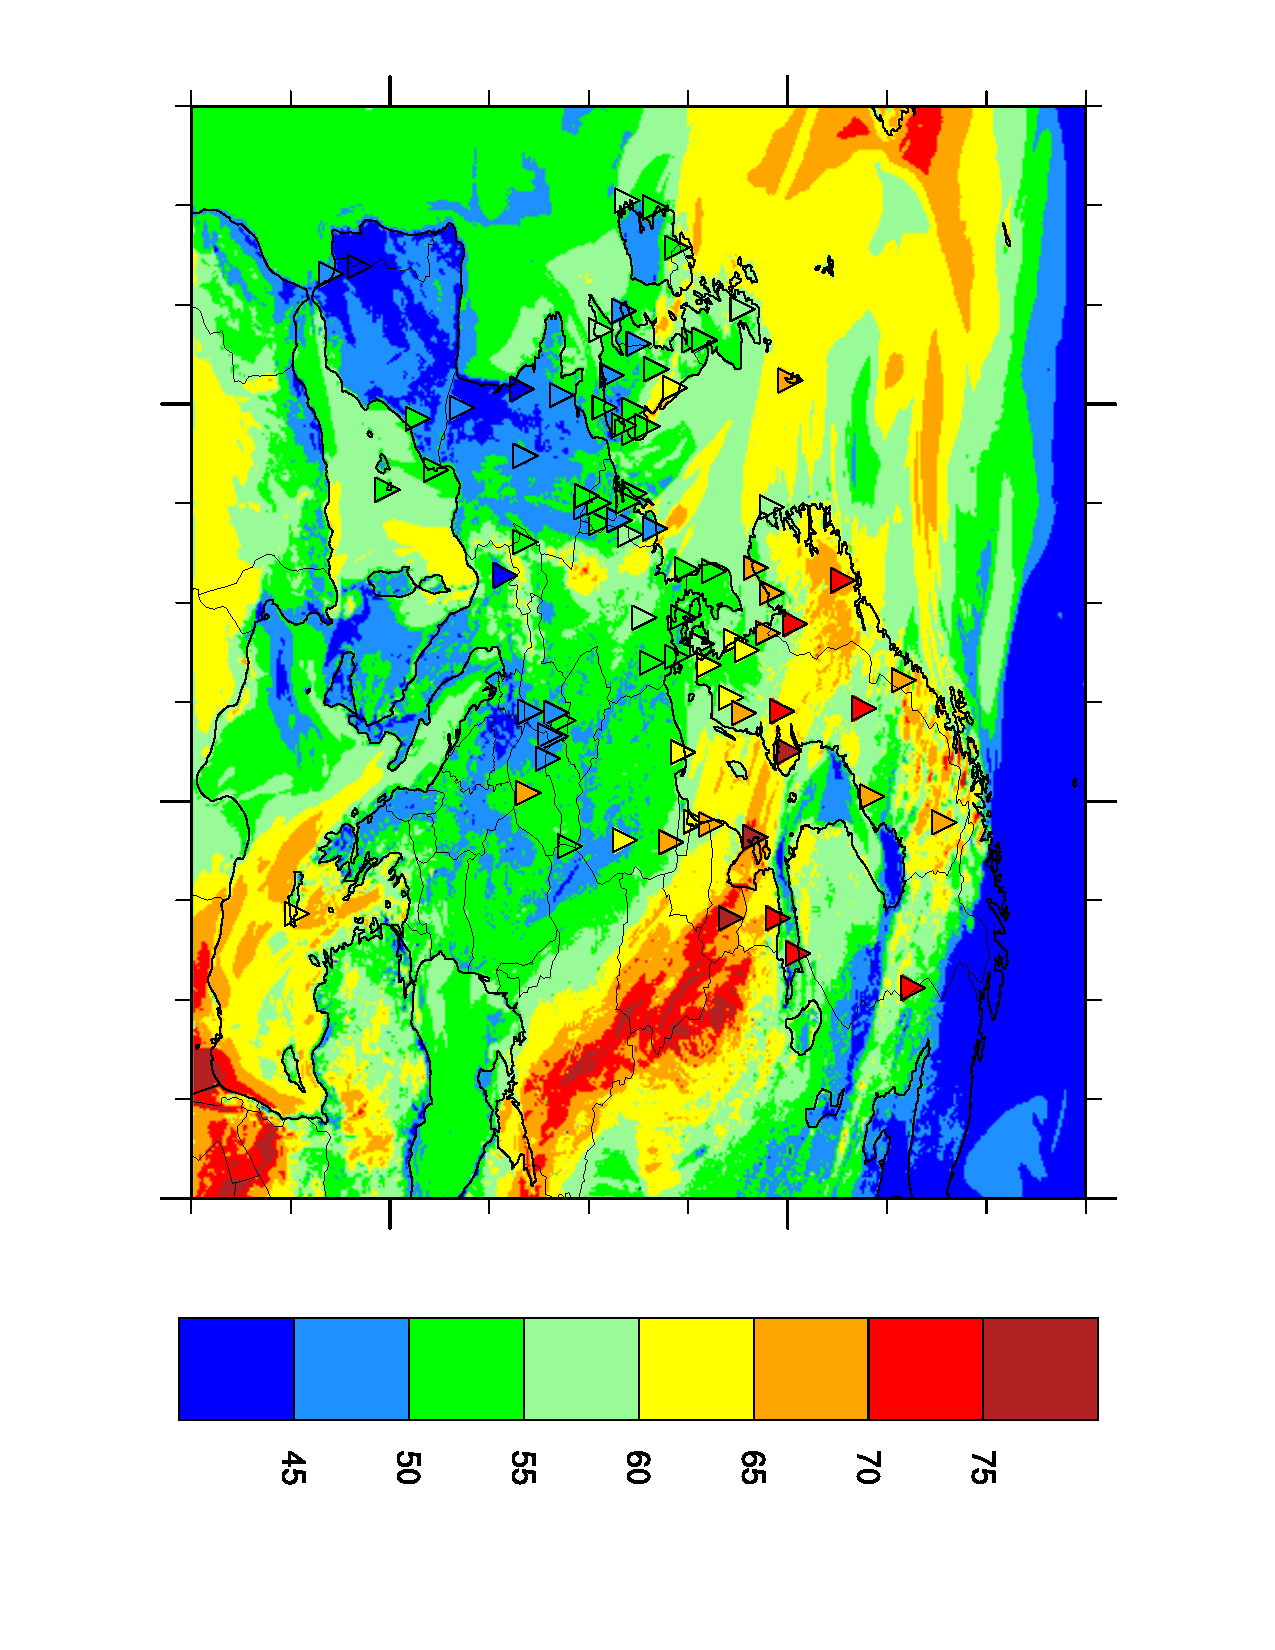
\includegraphics[clip=,angle=90,height=7.5cm,viewport=105 58 510 775]{FIGS_O3/20190424_MAXO3_ModObs_emep_H500.pdf}}
\caption{Modelled and measured daily max ozone [ppb] 24 April 2019.}
\label{fig:O3_20190424}
\end{figure}

The April episode was linked to a blocking high pressure located over western parts of Russia and Belarus, setting up southeasterly winds bringing warm and dry continental air masses northwards particularly to the Baltic countries, Scandinavia and parts of the UK. At 25 April Northern Norway registered the second highest surface ozone level (82 ppb) since the start of the monitoring in 1990. Likely, agricultural fires in East Europe (Ukraine and Russia) contributed to the peak ozone levels. The modelled and observed daily maximum ozone levels for 24 April are shown in Figure~\ref{fig:O3_20190424}. 

\begin{figure}[H]
  \centering{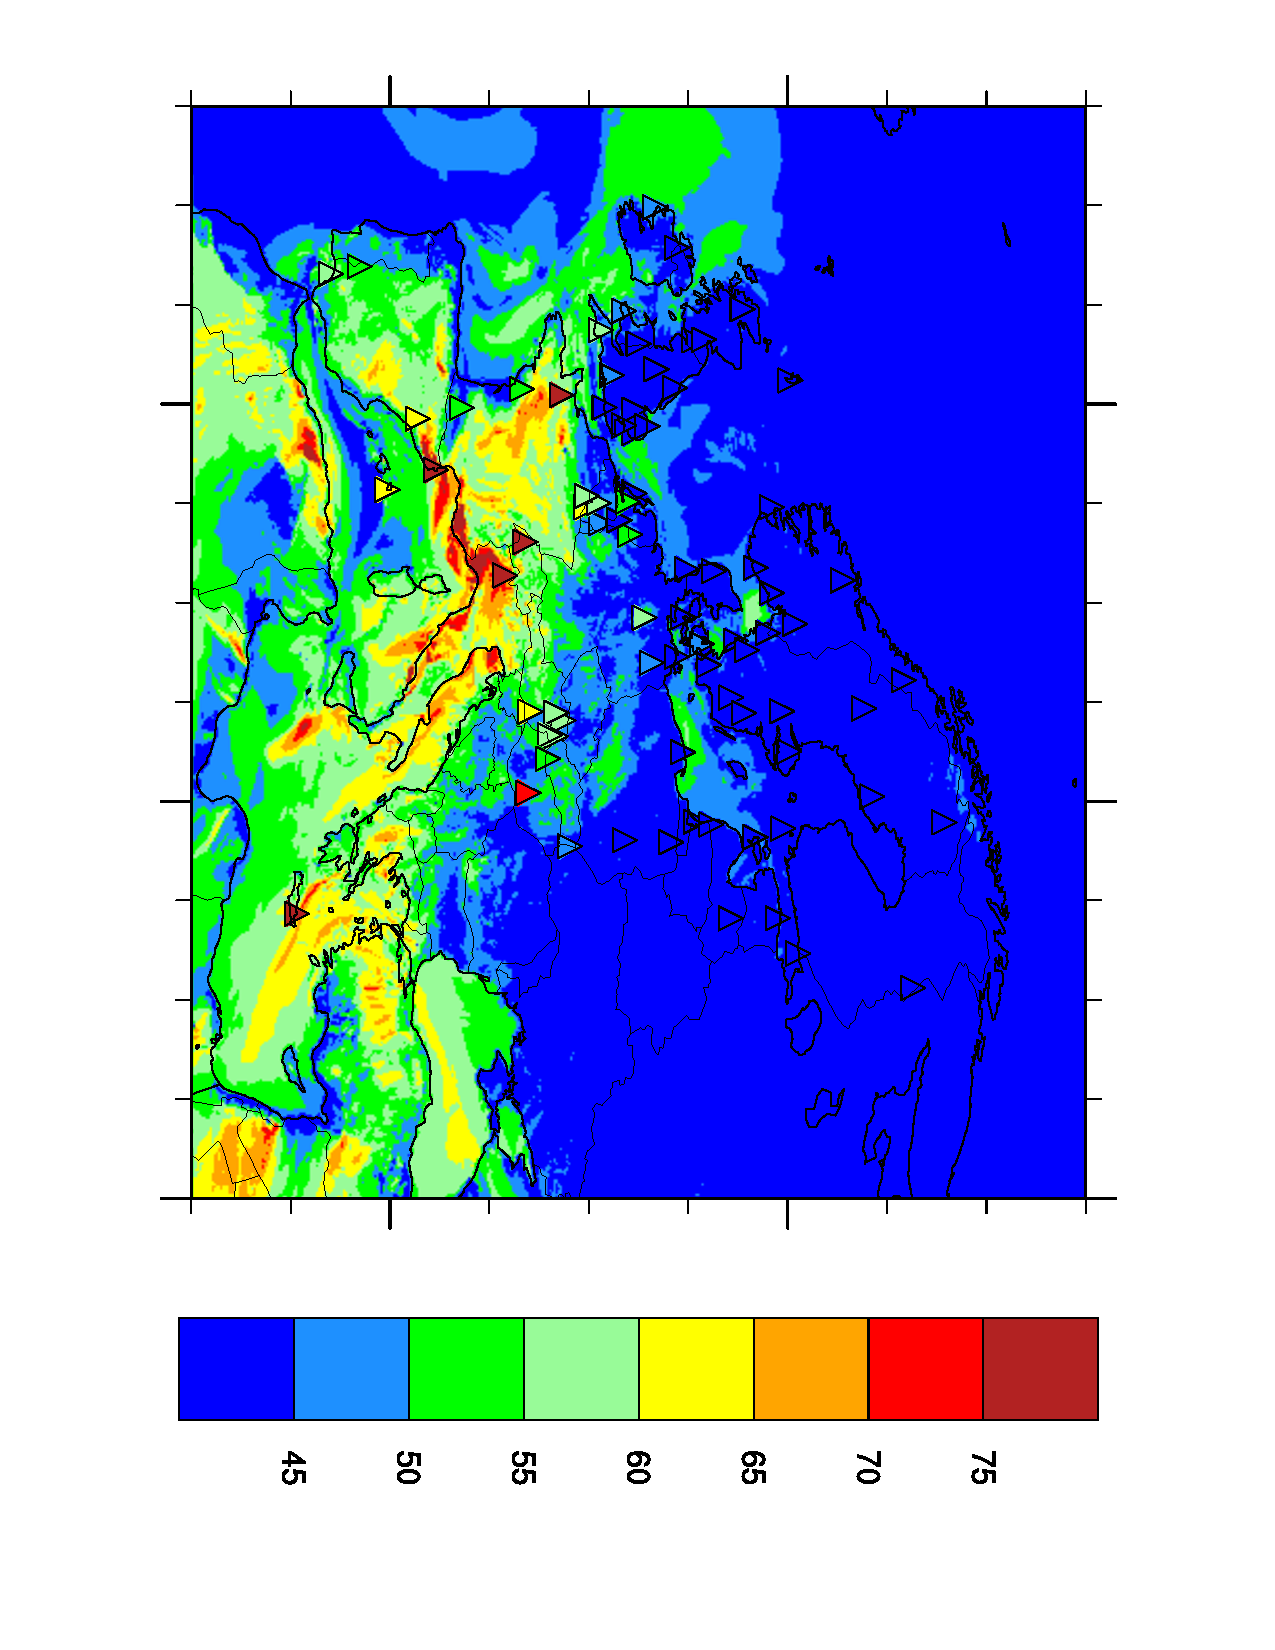
\includegraphics[clip=,angle=90,height=7.5cm,viewport=105 58 510 775]{FIGS_O3/20190628_MAXO3_ModObs_emep_H500.pdf}}
\caption{Modelled and measured daily max ozone [ppb] 28 June 2019.}
\label{fig:O3_20190628}
\end{figure}

June 2019 was the warmest June on record, globally as well as for Europe \citep{Bissolli:2020}. During 26-28 June a persistent high pressure over central Europe brought very hot air masses into central and western parts of the continent. In Germany, temperatures just below 40 \degrees C was observed and in France 13 stations surpassed France’s 2003 records, exceeding a temperature of 44.1 \degrees C. Surface ozone levels above EU's information threshold (180 \ug) were observed in many countries during this period. At Ispra in Italy an extreme level of 142 ppb (285 \ug) was reported on 28 June, breaking EU's alert threshold of 240 \ug. Figure~\ref{fig:O3_20190628} shows the modelled and observed daily maximum ozone levels for 28 June. 

\begin{figure}[H]
  \centering{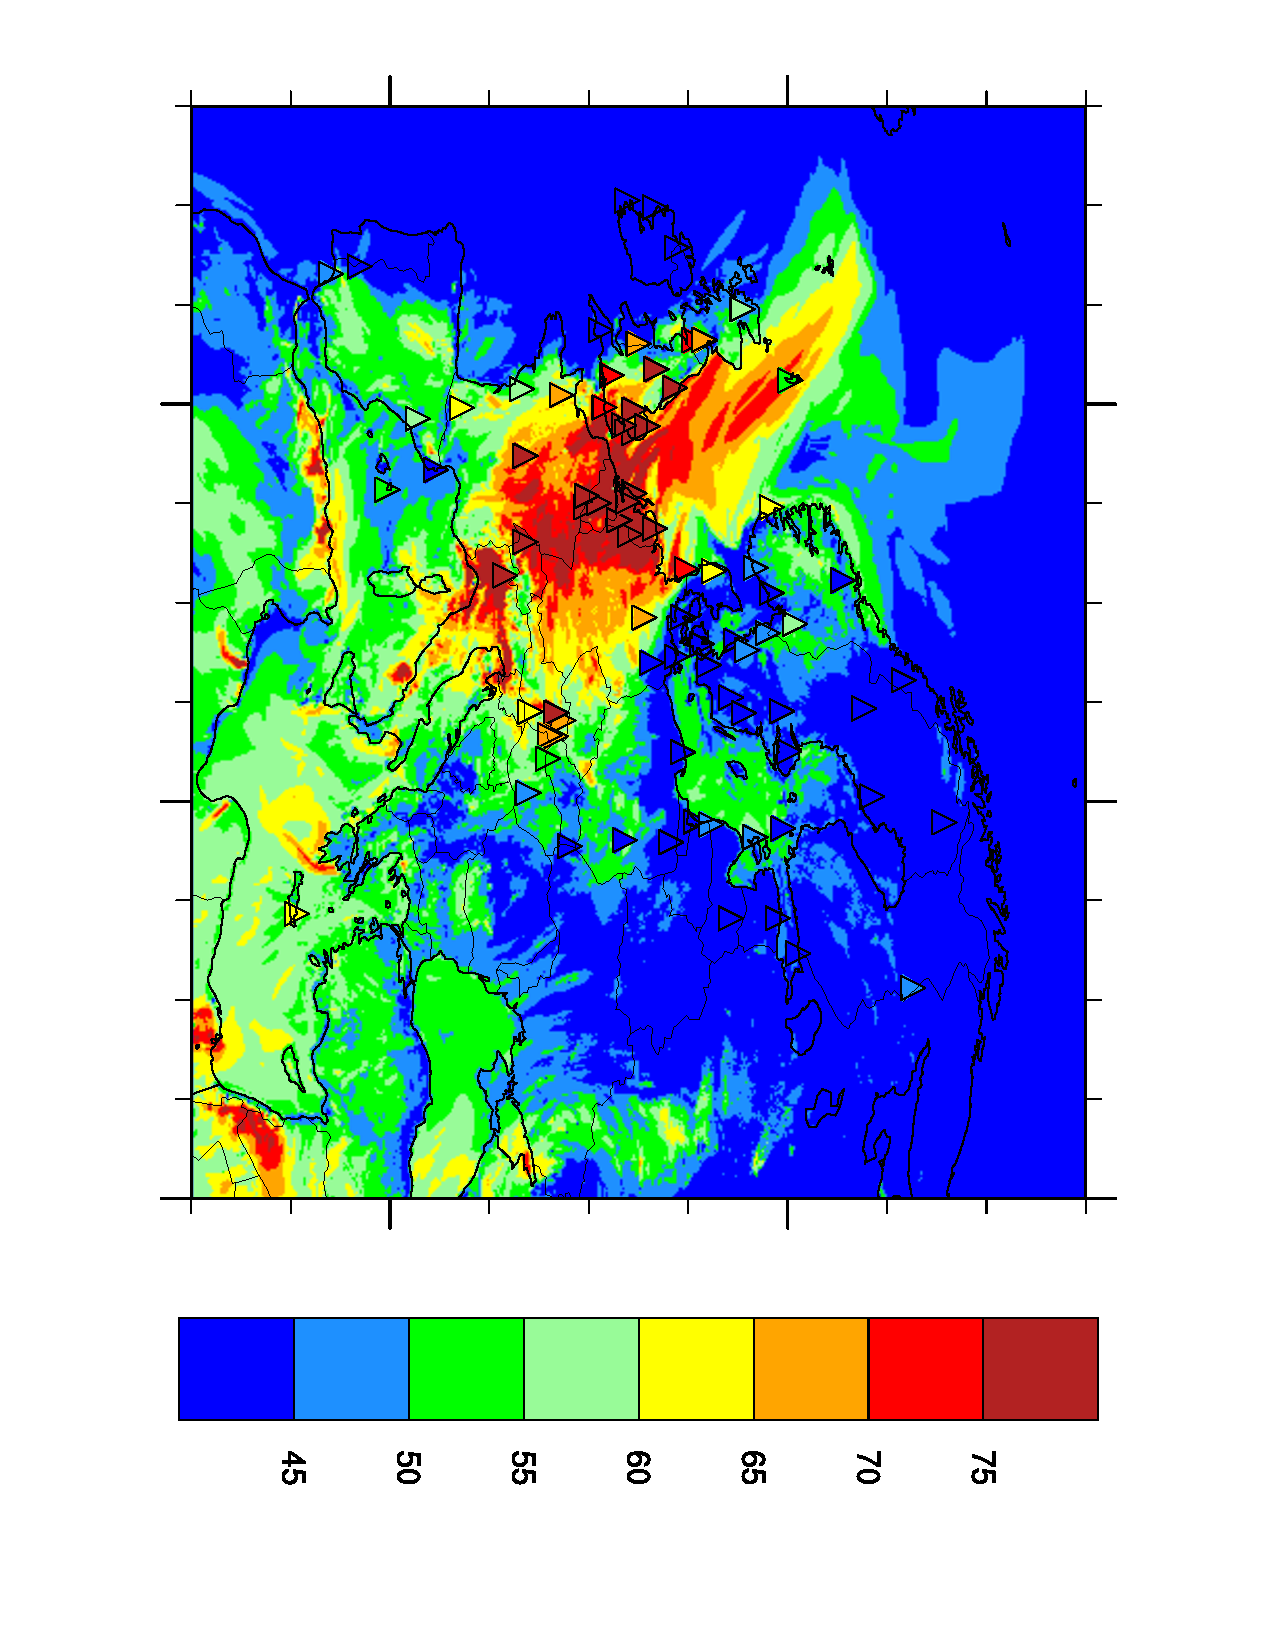
\includegraphics[clip=,angle=90,height=7.5cm,viewport=105 58 510 775]{FIGS_O3/20190725_MAXO3_ModObs_emep_H500.pdf}}
\caption{Modelled and measured daily max ozone [ppb] 25 July 2019.}
\label{fig:O3_20190725}
\end{figure}

One month later, during 24-26 July a new and even more intense (albeit shorter) heat wave struck central and northwestern part of Europe, and national temperature records were set in the UK and Germany (38.7 \degrees C in the UK and 40.5 \degrees C in Germany). Along with this heat wave, peak ozone levels were measured. In the UK, an hourly maximum level of 119 ppb (238 \ug) was observed at Sibton 25 July, the highest level measured at this site since 1996. At Vredepeel in the Netherlands, the ozone levels peaked at 127 ppb (254 \ug) on the same day and thereby broke EU's alert threshold. The extent of the ozone episode on 25 July is seen on Figure~\ref{fig:O3_20190725}, showing the modelled and observed values. 


For the year 2019 as a whole, Figure~\ref{fig:indicators_emep} shows various modelled ozone metrics with the corresponding measured metrics based on the EMEP measurement sites plotted on top of the maps. Only stations located below 500 metres above sea level were used in this comparison to avoid uncertainties related to the extraction of model data in regions with complex topography. Figure ~\ref{fig:indicators_emep} shows a) maxO3 (= mean of the daily max ozone concentration) for the 6-month period April-September, b) SOMO35 (= Sum of Ozone Means Over 35 ppb), c) AOT40 for forests (= Accumulated Ozone exposure over a Threshold of 40 ppb) for the 6-month period April-September using the hours between 08 and 20, and Figure~\ref{fig:indicatorPOD} shows POD$_1$ for forests (= Phytotoxic Ozone Dose above a threshold 1 mmol m$^{-2}$). Figure~\ref{fig:indicatorPOD} shows only modelled POD$_1$ since measurements could not be calculated from the ozone monitoring data directly and could not be included.

These plots indicate good agreement between these modelled and measured ozone metrics in general. The model and the measurements show an increasing gradient to the southeast as expected which reflects the strong dependency between surface ozone, temperature and solar radiation. 

\begin{figure}[H]
  \centering
  \subfigure[maxO3]{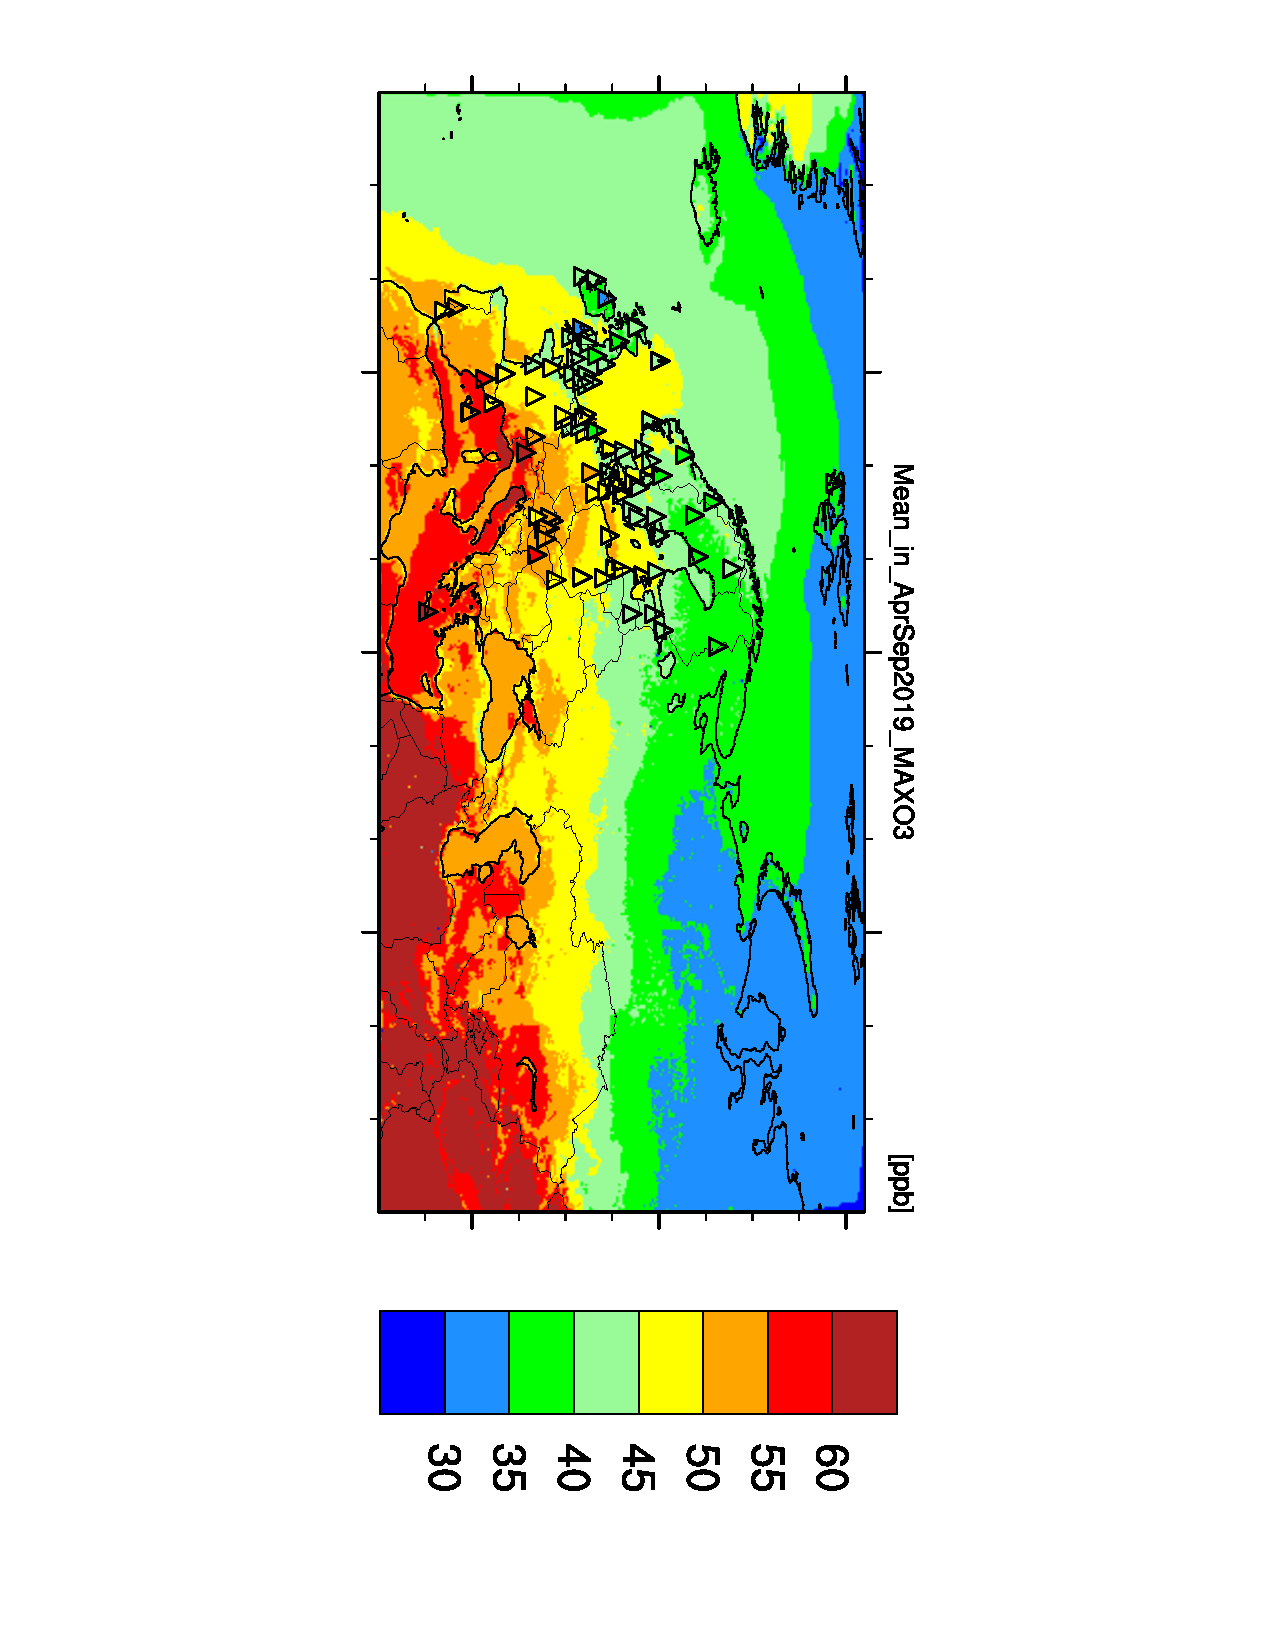
\includegraphics[clip=,angle=90,height=5.5cm,viewport=175 58 420 770]{FIGS_STATUS/MAXO3_AprSep_ModObs_emep_EMEP01.pdf}}
  \subfigure[SOMO35]{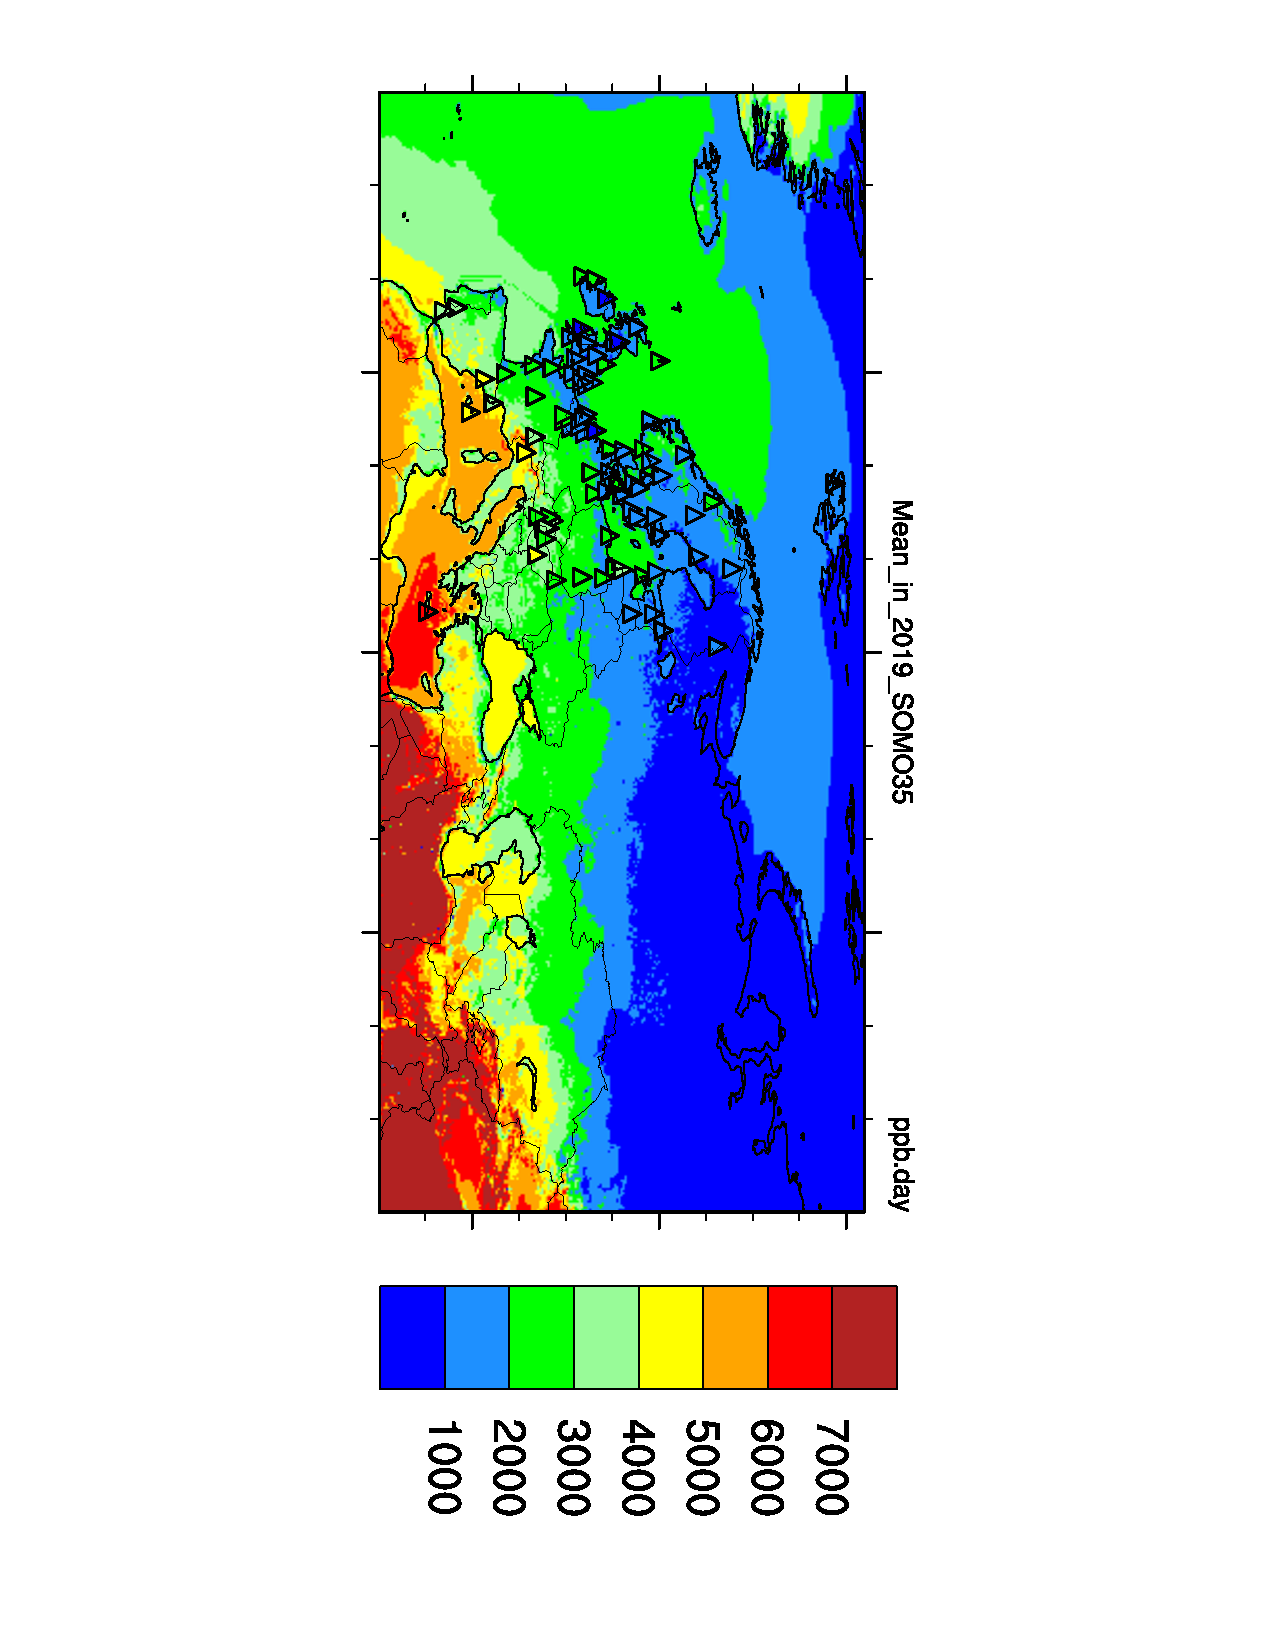
\includegraphics[clip=,angle=90,height=5.5cm,viewport=175 58 420 770]{FIGS_STATUS/SOMO35_ModObs_emep_EMEP01_L20EC.pdf}}
  \subfigure[AOT40]{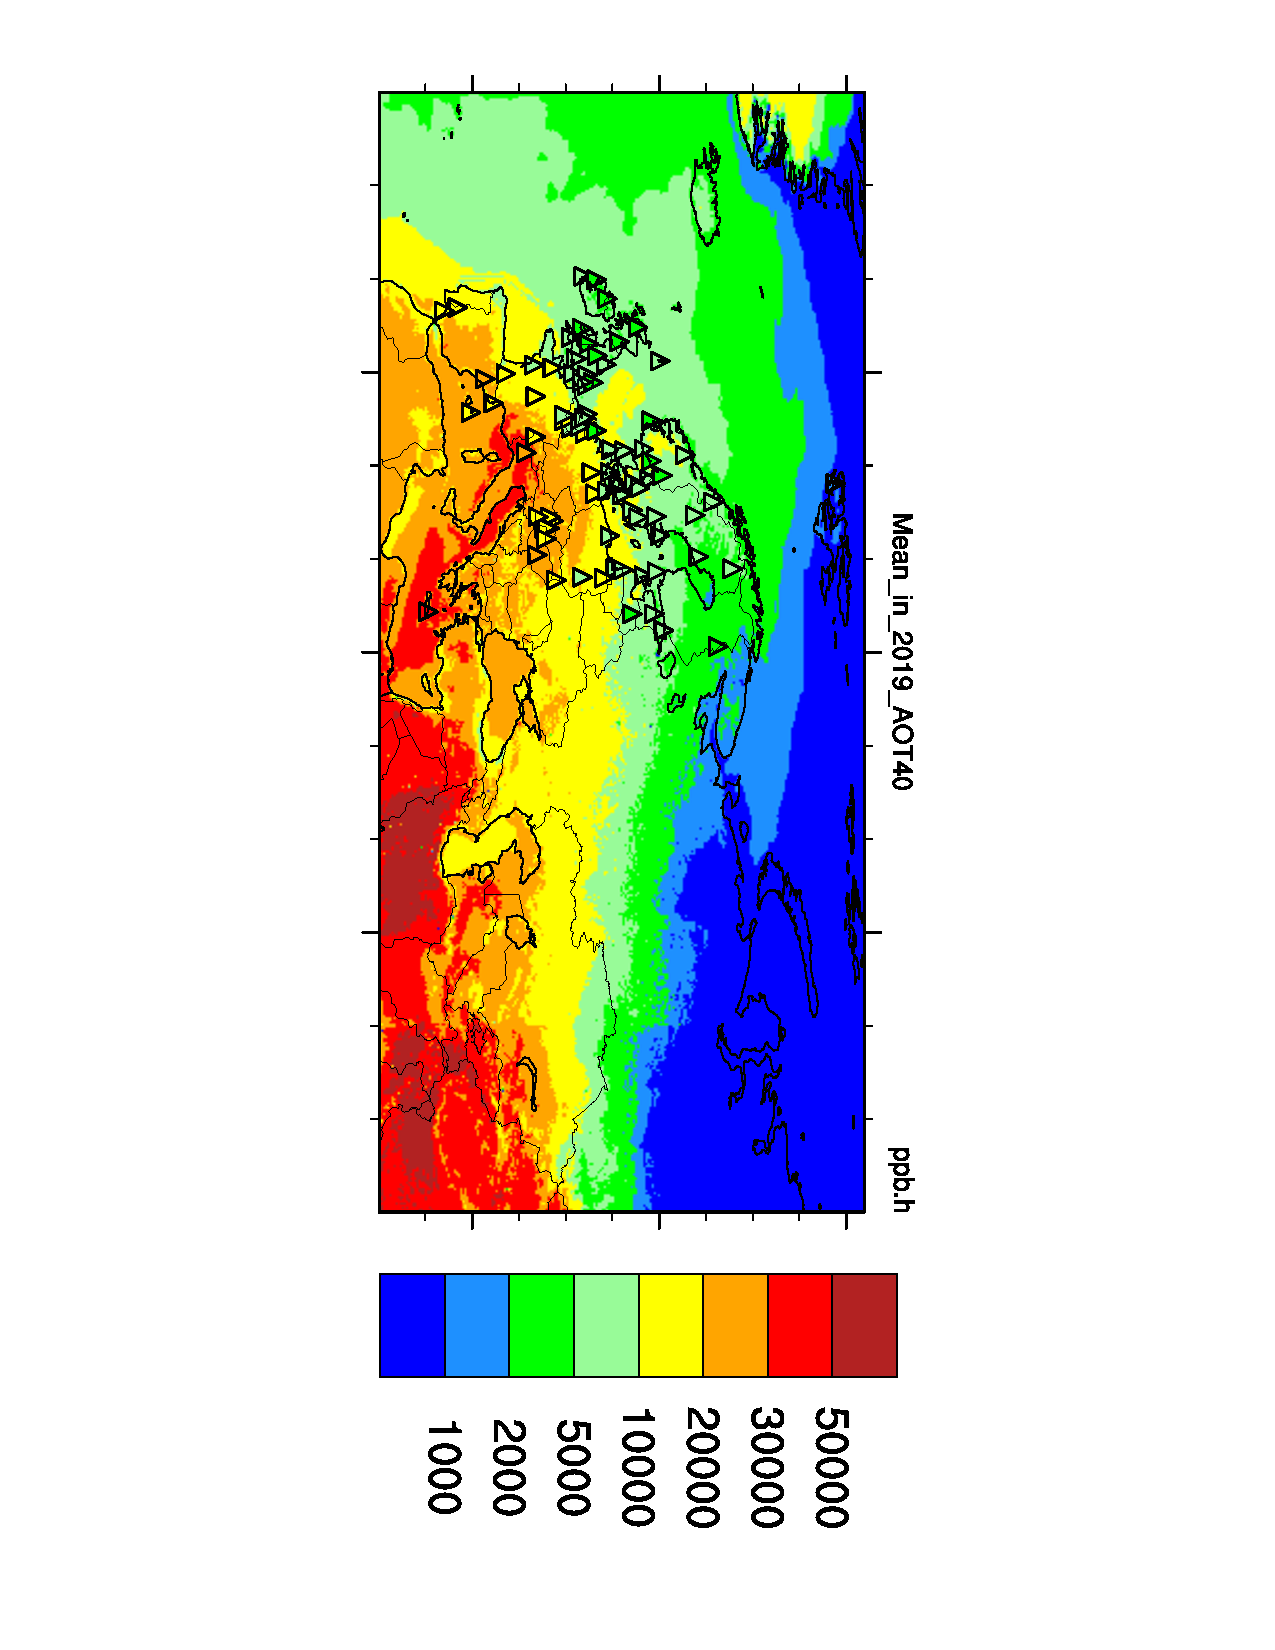
\includegraphics[clip=,angle=90,height=5.5cm,viewport=175 58 420 770]{FIGS_STATUS/AOT40_ModObs_emep_EMEP01_L20EC.pdf}}
\caption{Model results and observations at EMEP stations (triangles) for mean of daily maximum ozone concentrations (a) ([$ppb$], Apr-Sep), SOMO35 (b) [$ppb.d$] and AOT40 for forests (c) [$ppb.h$] in 2019. Only data from measurement sites below 500 m a.s.l. are shown.}
\label{fig:indicators_emep}
\end{figure}

\begin{figure}[H]
  \centering{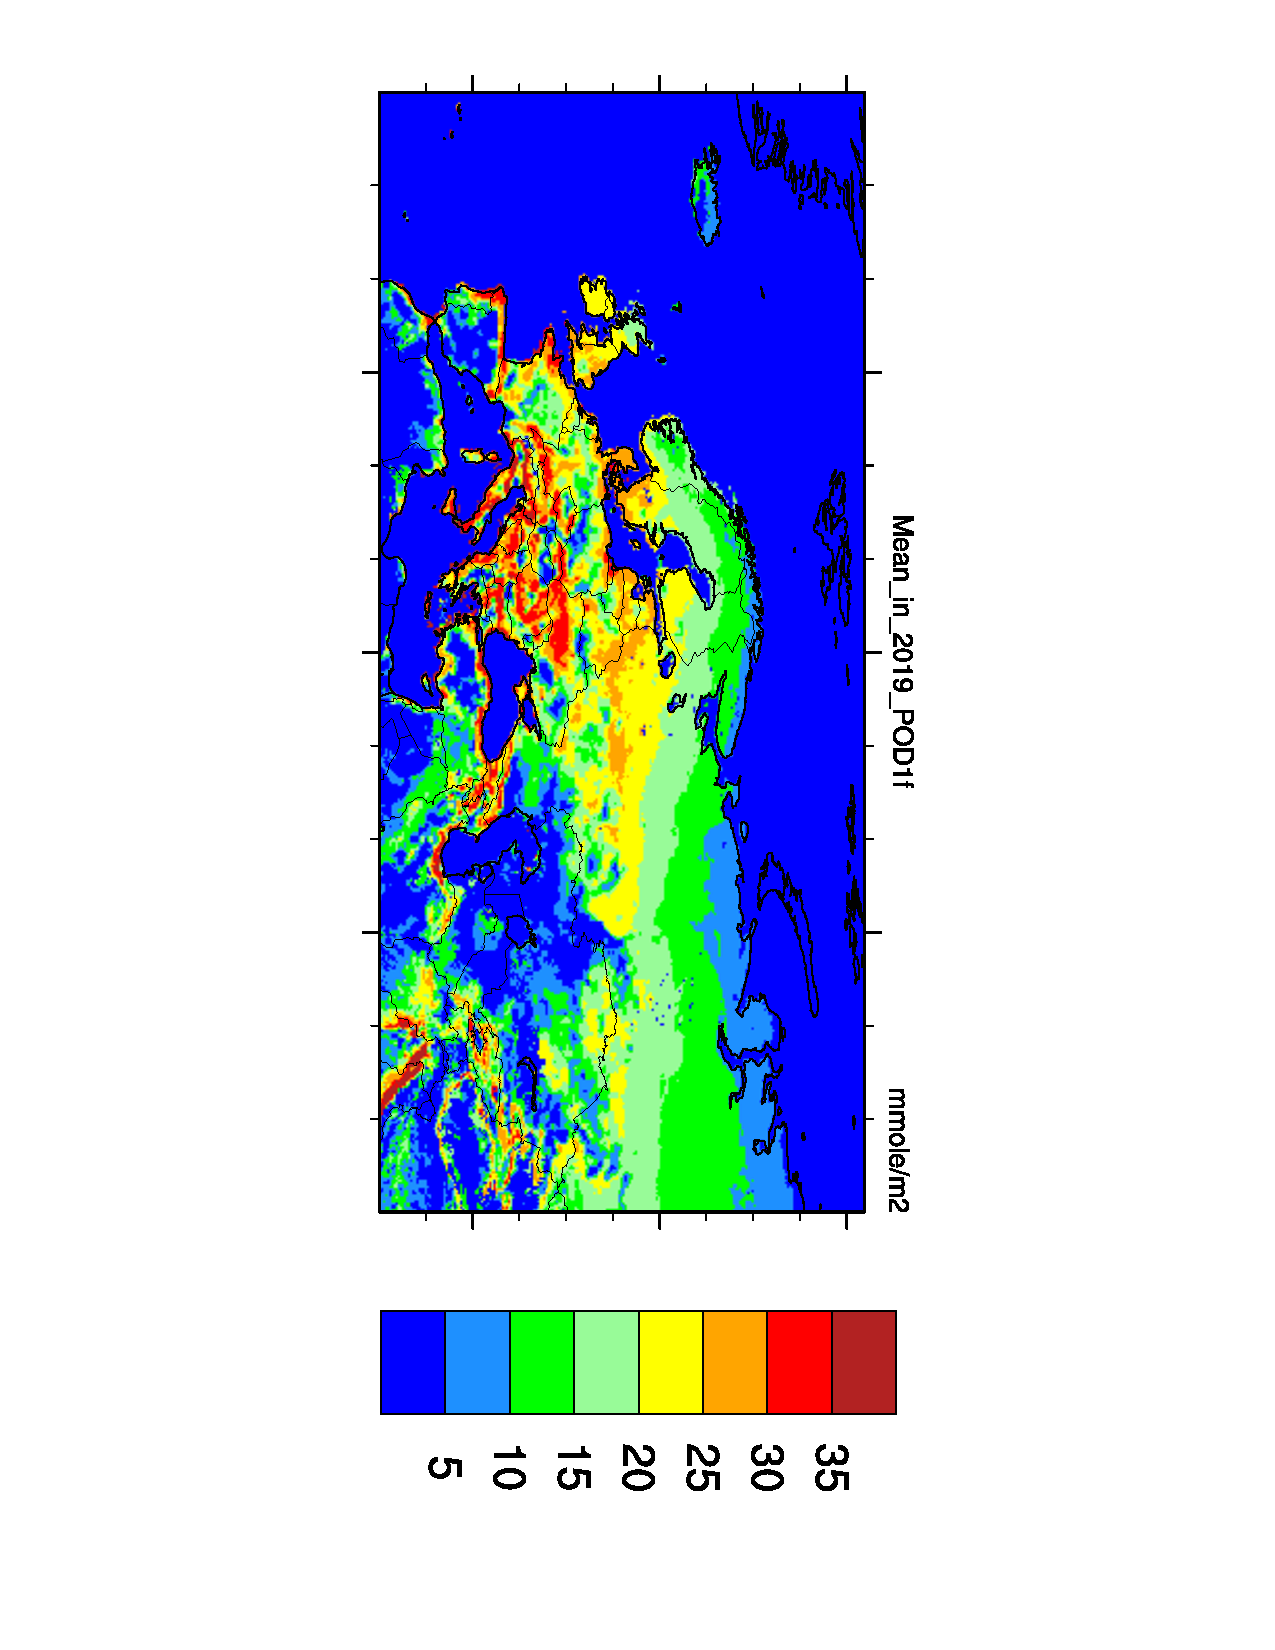
\includegraphics[clip=,angle=90,height=5.5cm,viewport=175 58 420 770]{FIGS_STATUS/POD1f_ModObs_emep_EMEP01.pdf}}
\caption{Model results of POD$_1$ for forests [$mmol m^-2$] in 2019}
\label{fig:indicatorPOD}
\end{figure}

It should be noted that the O$_3$ metrics such as AOT40 are very sensitive to the calculation of vertical O$_3$ gradients between the middle of the surface layer and the 3m height used for comparison with measurements \citep{Tuovinen:EP2007} and thus more difficult to compare with measurement data than, e.g., the mean daily maximum. Indeed, the formulation we use \citep{Simpson:EMEP2012} is probably better suited to a lowest model layer of 90m thickness (since we equate the centre of this, ca. 45m, with a `blending-height') than to a lowest model layer of 50m thickness (as used throughout this report). 
The modelled POD$_1$ pattern differs from the other metrics reflecting the influence of additional parameters such as plant physiology, soil moisture etc., and is a metric more indicative of the direct impact of ozone on vegetation than, e.g., AOT40. The POD$_1$ field could, however, not be validated by the EMEP ozone measurement data alone. 

SOMO35 is an indicator for health impacts recommended by WHO, and the results given in Figure~\ref{fig:indicators_emep} indicate that the health risk associated with surface ozone increased towards southern Europe. Highest levels are seen in the Mediterranean area and Northern Italy. SOMO35 is a health risk indicator without any specific threshold or limit value.

AOT40 and POD$_1$ are indicators for effects on vegetation. UNECE's critical level for forests based on the 6-months AOT40 value is 5000 ppb hours, and the results shown in Figure~\ref{fig:indicators_emep} indicate that this level was exceeded in most of Europe in 2019 although the model tends to overestimate the AOT40 values somewhat. In parts of central and south Europe the critical level was exceeded by a very large margin (20000 ppb hours and more). During dry periods, plants will reduce or close their stomata as a response to soil water deficit, which in turn will lead to reduced uptake of ozone.  Parts of the reason for the elevated atmospheric concentrations of ozone (and the high AOT40 levels) could thus be explained by the reduced uptake in vegetation.

On the contrary, POD$_1$ takes into account this soil moisture deficit, giving an estimate of the actual flux of ozone into the plants. It is interesting to see the substantial difference in the geographical pattern of AOT40 and POD$_1$ in Figures~\ref{fig:indicators_emep} (c) and \ref{fig:indicatorPOD}. Whereas AOT40 shows a north-south gradient with peak values over southern/central parts of the continent, POD$_1$ is highest along the coast and shows a minimum in central parts of Europe just where high values of AOT40 are seen. This reflects the importance of the soil moisture effect for these two metrics for ozone damage to vegetation. For POD$_1$ the limit value depends on the species and Mills et al (2011) give a value of 4 mmol m$^{-2}$ for birch and beech and 8 mmol m$^{-2}$ for Norway spruce. The results in Figures~\ref{fig:indicators_emep} (c) and \ref{fig:indicatorPOD} indicate that both these limit values were exceeded in most of Europe. The modelled levels of POD$_1$ could, however, not be validated by observations. 

Surface ozone levels and the associated metrics were fairly high in 2019 which partly could be explained by several heat waves striking the continent in the summer half year. This is an indication of the strong link between climate and surface ozone and raises the issue of climate induced changes of ozone in the years to come. A main question is to what extent such changes will outweigh the benefits of reduced ozone precursors emissions. 


%=========================================
\subsection{Particulate matter} 
\label{subs:PMstatus}

Maps of annual mean concentrations of \PM[10] and \PM[2.5] in 2019,
calculated by the EMEP MSC-W model, are presented in
Figure~\ref{fig:PMin2019}. The figures also show annual mean \PM[10]
and \PM[2.5] concentrations observed at the EMEP monitoring network,
which are represented by colour triangles overlaying the contours of the
modelled concentration fields.

\begin{figure}[H]
  \centering{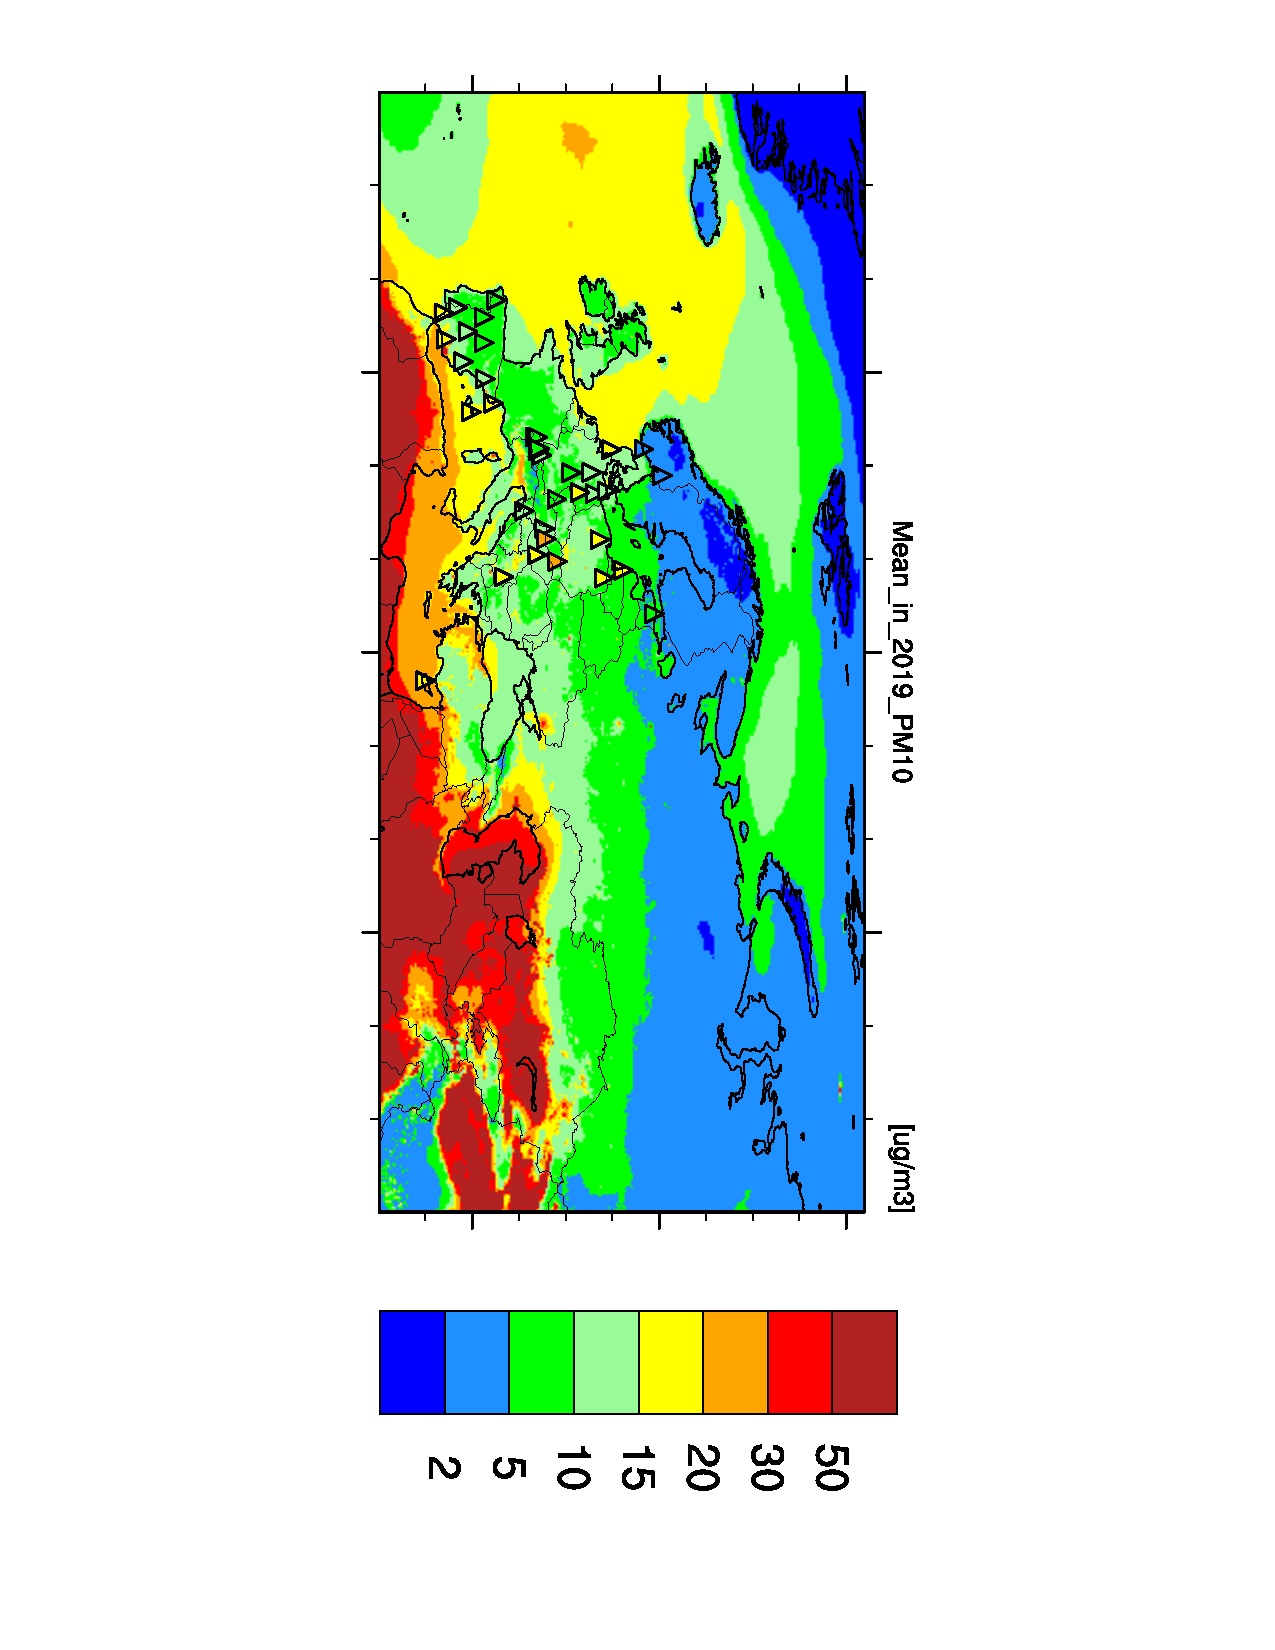
\includegraphics[clip=,angle=90,height=6cm,viewport=175 67 448 754]{FIGS_PM/Mean_in_2019_PM10_EMEP01_ALL.pdf}}\\
  \vspace{0.5cm}
  \centering{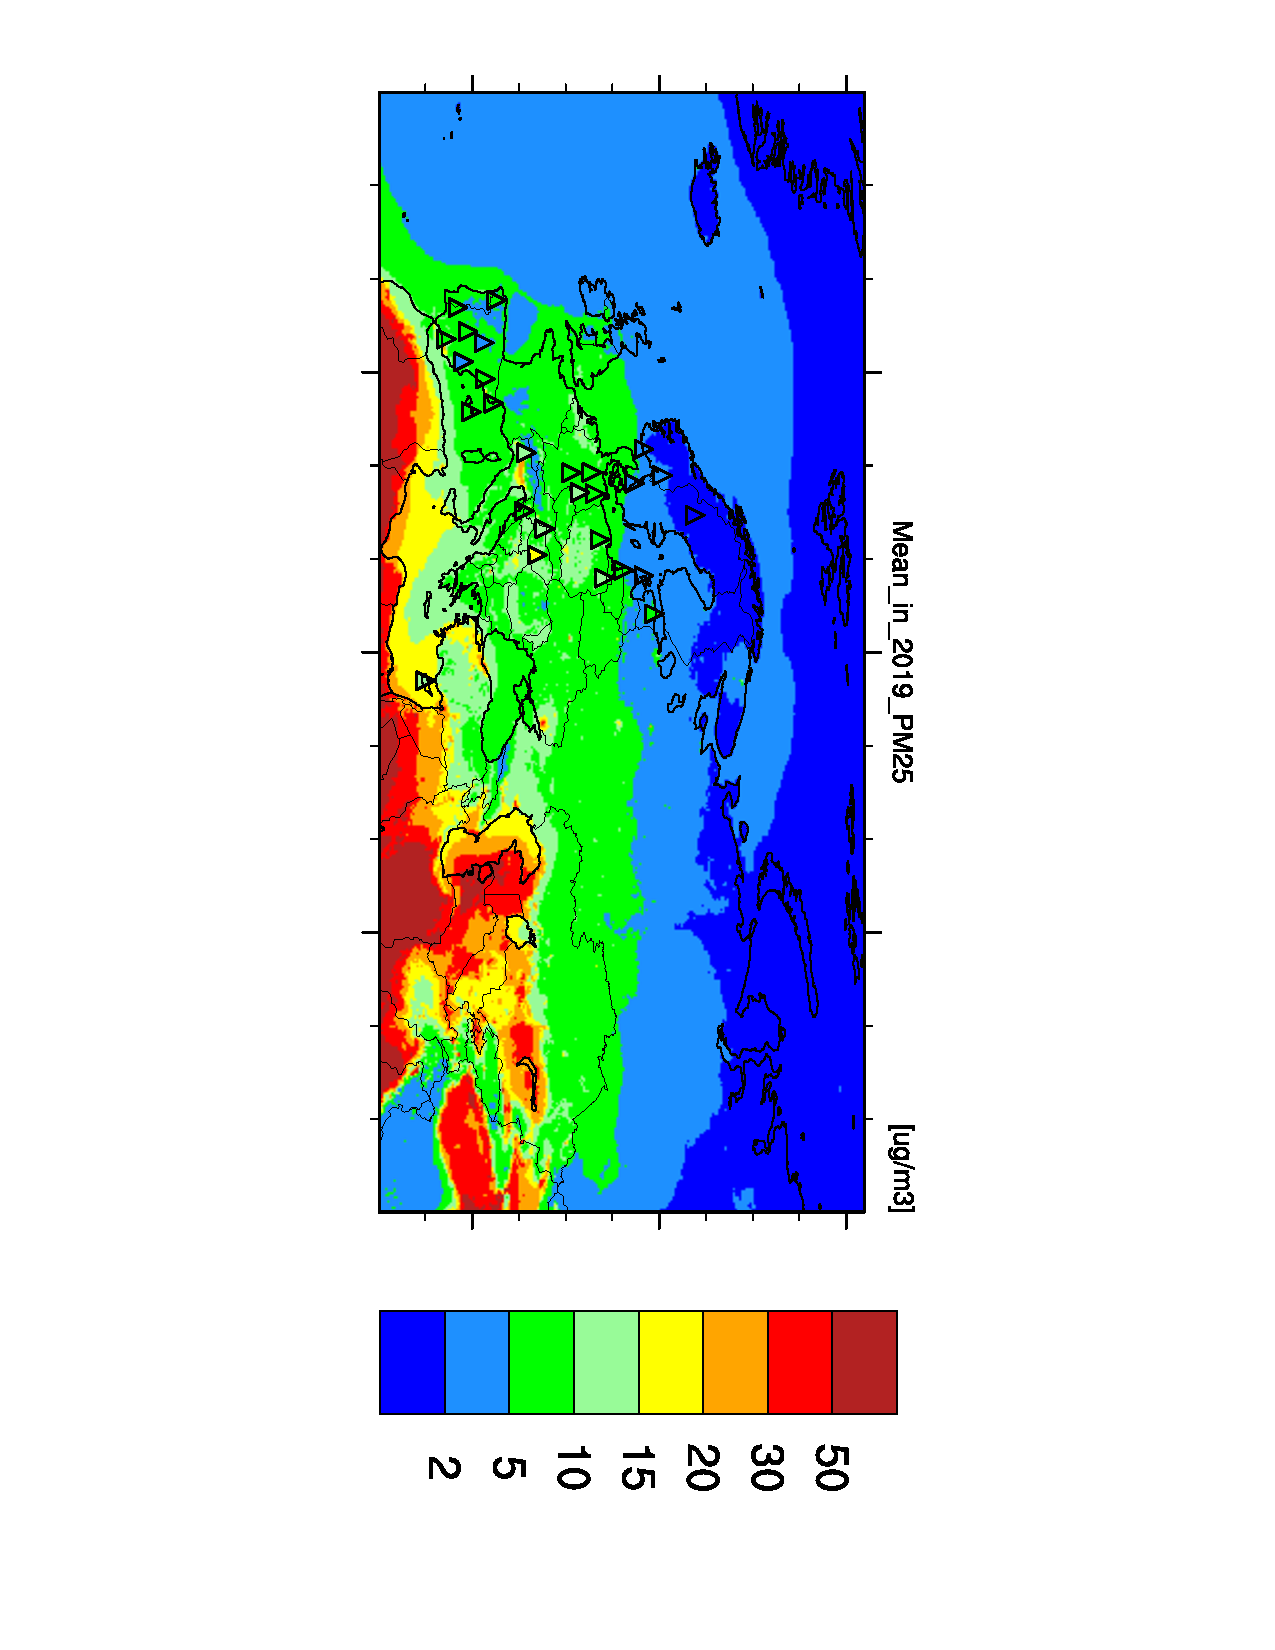
\includegraphics[clip=,angle=90,height=6cm,viewport=175 67 448 754]{FIGS_PM/Mean_in_2019_PM25_EMEP01_ALL.pdf}}
\caption{Annual mean concentrations of \PM[10] and \PM[2.5] in 2019:
  calculated with the EMEP MSC-W model (colour contours) and observed
  at EMEP monitoring network sites (colour triangles). \textit{Note:
    Observations include hourly, daily and weekly data.}}
\label{fig:PMin2019}
\end{figure}


The model results and the observations are well in agreement
regarding the geographical distribution of the annual mean levels of
\PM[10] and \PM[2.5], showing their general increase over land from
north to south. The concentrations are below 2-5 \ug in Northern
Europe, increasing to 5-15 \ug in the mid-latitudes and further south,
\PM[2.5] levels being somewhat lower than those of
\PM[10]. Figure~\ref{fig:PMin2019} displays fairly homogeneous modelled levels of regional background PM over most of Central and Western Europe,
with \PM[10] in excess of 20 \ug in the Po Valley and on Cyprus. The observations also show \PM[10] concentrations above 20 \ug in Slovakia. \PM[2.5] concentrations are below 10 \ug over most of EMEP domain (except the most south/southeastern regions), or otherwise between 10 and 15 \ug in  parts of Benelux, Poland, Hungary and some Balkan countries. The only site with observed annual mean \PM[10] above 15 \ug (namely 16.3 \ug) was Hungarian K-Puszta. Furthermore, the model calculates high PM for the regions east of the Caspian Sea (parts of Kazakhstan, Uzbekistan, Turkmenistan) and over the southern Mediterranean, with annual mean concentrations in excess of 50 \ug. These high PM concentrations are due to windblown dust from the arid soils and deserts of Central Asia, though the precision of the calculated values still cannot be verified due to the lack of observations in these regions.

There is a good agreement between the modelled and observed
distributions of annual mean \PM[10] and \PM[2.5], with correlation
coefficients of 0.60 and 0.72, respectively. Overall, the model
underestimates the observed annual mean of \PM[10] by 12\% and
\PM[2.5] by 13\% (see also Table \ref{tab:tableOldFashioned} in \ref{ch:appx_modeleval}). \textcolor{blue}{CHECK with and Refer to AeroVal....}


Overall, the year of 2019 was quite moderate with respect to PM air pollution in Europe, which was due to dominating meteorological conditions that year. It was relatively warm across the EMEP area (Figure~\ref{fig:metyear-avMET}), in particular in the cold half-year (Figure~\ref{fig:temp-avMET}). Mild winter conditions would mean less need for residential heating, resulting in lower emissions from this sector. Moreover, stagnant air conditions (with temperature inversion, low wind speed and thin mixing layer), typically causing elevated pollution levels, are less frequent in warm winters. Also, the spring/summer period was relatively warm (except from Russia, Kazakhstan, Finland, most of Sweden, Spain and Portugal). During those months, the higher temperatures would enhance evaporation of semi-volatile inorganic and organic aerosols (SIA and SOA), though the more efficient oxidation contributes to secondary aerosol formation. Furthermore, the year 2019 was relatively dry over most of Europe (except in the south and parts of Scandinavia), in EECCA countries, and most of Russia (except for the northern regions), as shown in Figure~\ref{fig:metyear-avMET}. However, the amount of precipitation was also relatively large in the cold half-year in Denmark, France, the UK and parts of Germany (Figure~\ref{fig:prec-avMET}). As documented in ~\citet{CAMS2020}, the wet end of the year in western and southern Europe was the most prominent feature of precipitation in 2019, with 
November being particularly extreme, both in terms of the total rainfall amounts and the number of days with heavy rainfall. As wet scavenging is the main PM removal mechanism, this, combined with the mild winter temperatures, resulted in the lower levels of PM pollution in winter 2019 over most of Europe.   

Figure~\ref{fig:PManomin2019} presents the relative anomalies of mean \PM[10] and \PM[2.5] concentrations in 2019 relative to 2000-2018 averages, based on the 2000-2019 trend runs performed with the EMEP MSC-W model using a consistent emission data-set based on officially submitted data, as documented in Ch \ref{ch:Trends}. In order to look at the sole effect of meteorological conditions on PM pollution, also the 2019 run used here is based on the reported emissions and thus different from the 2019 Status run (in which TNO's emissions for residential combustion are used, as documented in Ch \ref{Mod_2019}). Figure~\ref{fig:PManomin2019} shows that the PM pollution in 2019 was relatively moderate, with annual mean concentrations being 5-20\% lower than the 2000-2018 averages over most of the EMEP domain, and 20-35\% lower compared to the 18-year average in Central Europe and over vast areas in the N/NE of Russia. Only along NW/N coasts in Fennoscandia, parts of Spain and some south-eastern regions (parts of Turkey, the Caucasus region and Central Asian countries), \PM[10] and \PM[2.5] levels in 2019 were higher relative to the 2000-2018 averages. 

%\begin{figure}[H]
%  \centering{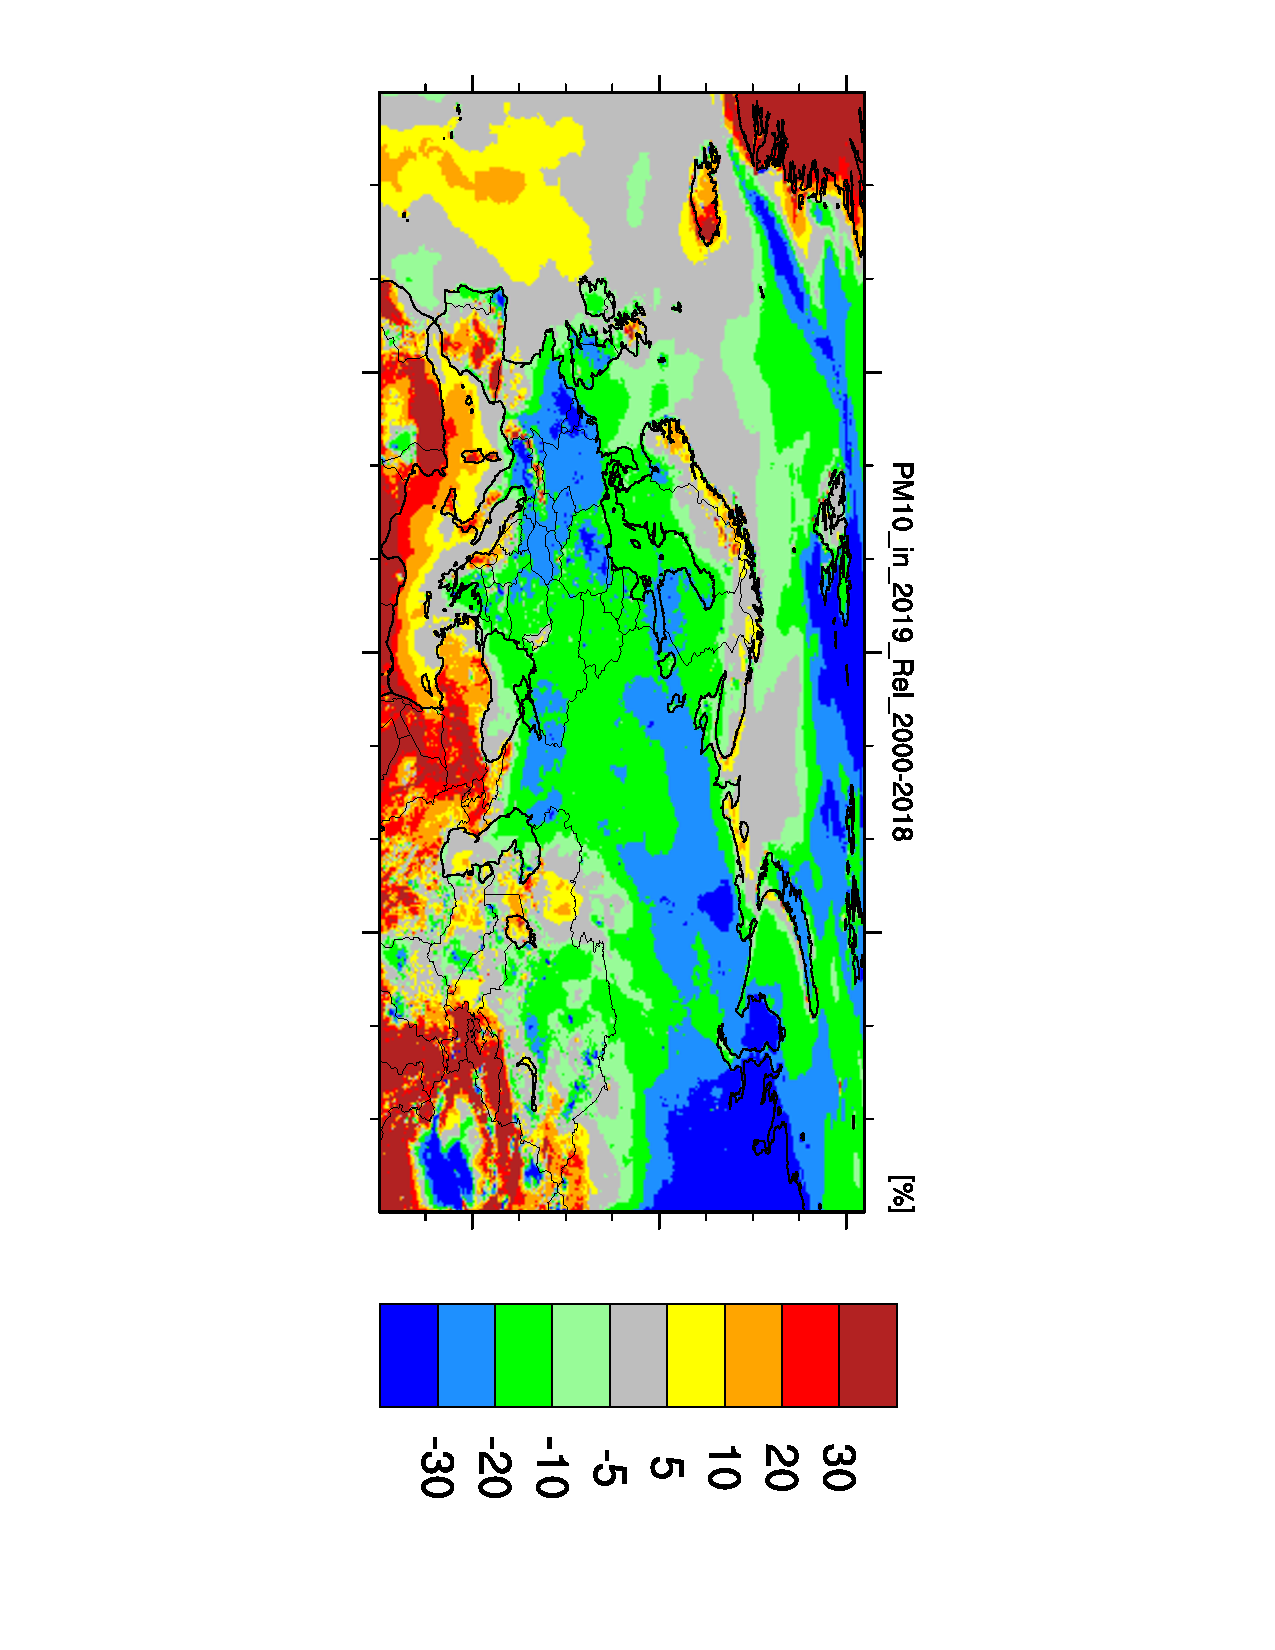
\includegraphics[clip=,angle=90,height=3cm,viewport=175 67 448 754]{FIGS_PM/RelAnomaly_PM10_2019_vs_2000-2018.pdf}}
%  \centering{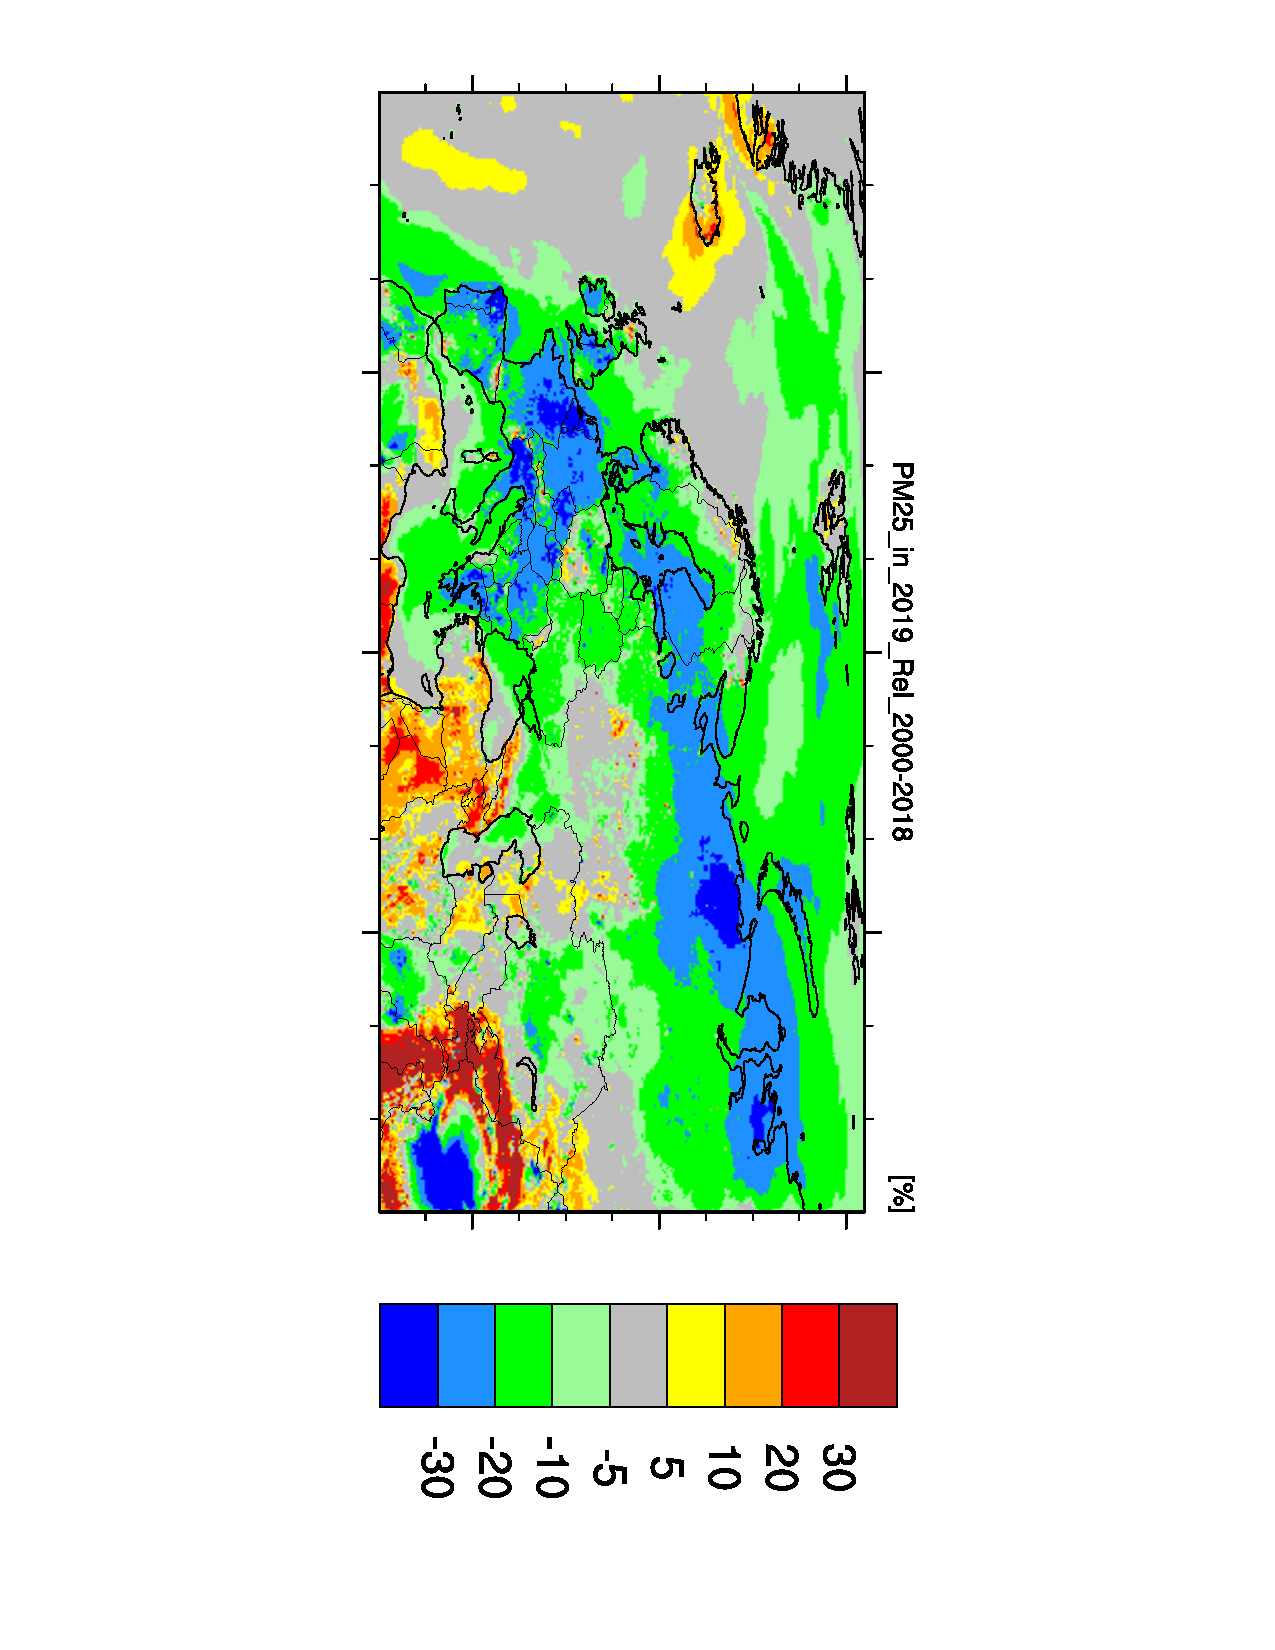
\includegraphics[clip=,angle=90,height=3cm,viewport=175 67 448 754]{FIGS_PM/RelAnomaly_PM25_2019_vs_2000-2018.pdf}}
%\caption{Relative anomalies of mean \PM[10] and \PM[2.5] in 2019 from the 2000-2018 mean.}
%\label{fig:PManomin2019}
%\end{figure}

\begin{figure}[H]
  \centering{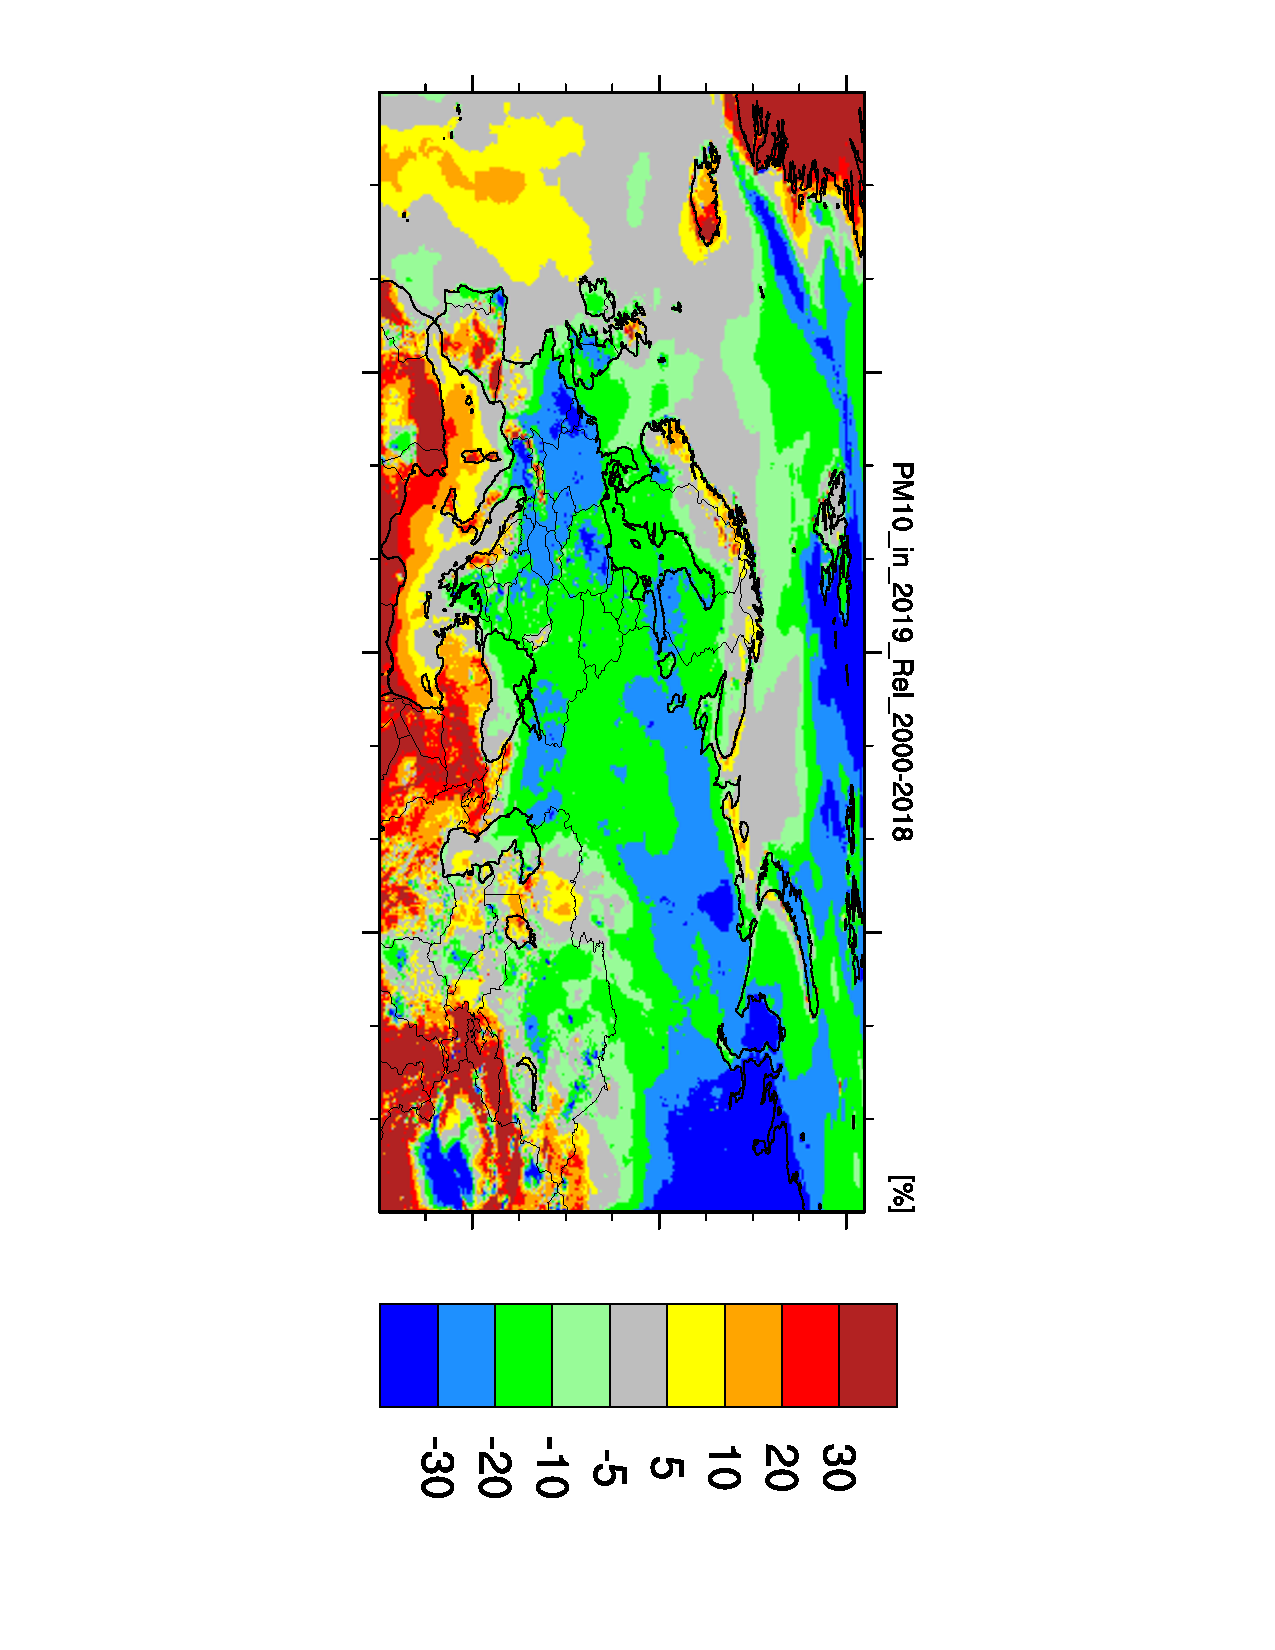
\includegraphics[clip=,angle=90,height=5.9cm,viewport=175 67 448 754]{FIGS_PM/RelAnomaly_PM10_2019_vs_2000-2018.pdf}}
  \vspace{0.5cm}
  \centering{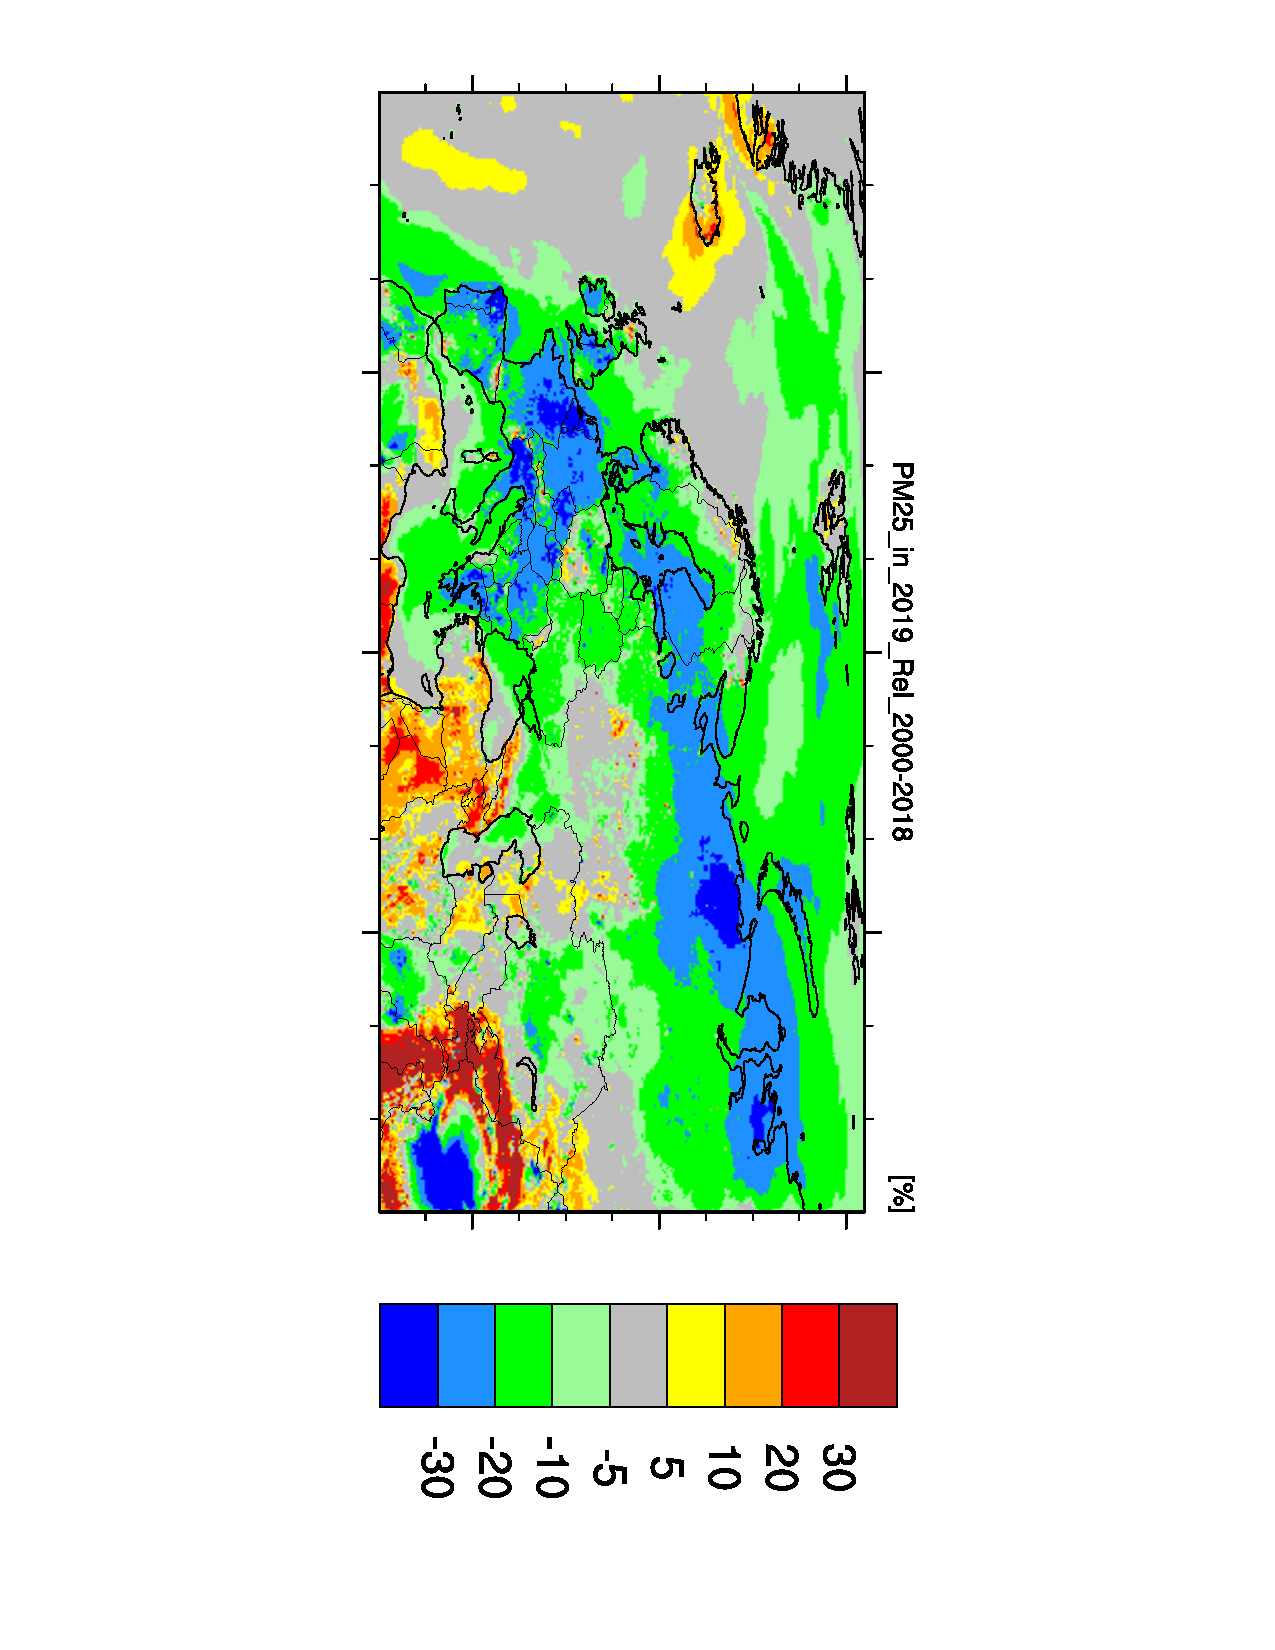
\includegraphics[clip=,angle=90,height=5.9cm,viewport=175 67 448 754]{FIGS_PM/RelAnomaly_PM25_2019_vs_2000-2018.pdf}}
\caption{Relative anomalies of mean \PM[10] and \PM[2.5] in 2019 from the 2000-2018 mean.}
\label{fig:PManomin2019}
\end{figure}



\subsubsection[PM exceedances]{Exceedances of EU limit values and WHO Air Quality Guidelines in 2019}
\label{subsec:PMexc}

In this section we compare \PM[10] and \PM[2.5] exceedances
of EU critical limits and WHO recommended Air Quality
Guidelines \citep{WHO:AQG}, calculated by the EMEP MSC-W model, with
those measured at EMEP sites. The EU limit values (Council 
Directive 1999/30/EC) for \PM[10] are 40 \ug for the annual mean and 50 \ug for
the daily mean concentrations, with the daily limit not to be exceeded
more than 35 times per calendar year~\citep{EU2008}. For \PM[2.5], the
annual mean limit value of 25 \ug entered into force on 01.01.2015.

The Air Quality Guidelines (AQG) recommended by WHO \citep{WHO:AQG}
are:
\begin{itemize}
\item for \PM[10]: 20 \ug annual mean, 50 \ug 24-hourly (99th perc. or 3 days per year)
\item for \PM[2.5]: 10 \ug annual mean, 25 \ug 24-hourly (99th perc. or 3 days per year)
\end{itemize}


The EU limit values for protection of human health from particulate
matter pollution and the WHO AQG for PM should apply to concentrations
for zones or agglomerations, in rural and urban areas,
which are representative for exposure of the general
population. \PM[10] and \PM[2.5] concentrations calculated with the
EMEP MSC-W model on the 0.1$\degrees \times$ 0.1$\degrees$ grid cannot
reproduce urban hotspot levels, but give a reasonable representation
of PM levels occurring in rural and, to some extend, in urban background
areas.


Model results and EMEP observational data show that the annual mean \PM[10] concentrations were below the EU limit value of 40 \ug for all of Europe in 2019 (Figure~\ref{fig:PMin2019}). The model calculates annual mean \PM[10] above the WHO recommended AQG of 20 \ug
for only small regions in the Po Valley and western Turkey. The highest
observed annual mean \PM[10] concentrations, exceeding the AQG of 20 \ug, were registered at Slovakian sites (24 \ug at SK0004 and 23 \ug SK0007) and Greek GR0001 (23 \ug, 58\% data coverage only). Further, the observations and model results show that annual mean \PM[2.5] concentrations (Figure~\ref{fig:PMin2019}) in 2019 were below the EU limit value of 25 \ug (except in the Po Valley according to the model). However, there were observed cases of exceedance of the WHO AQG value of 10 \ug by annual mean \PM[2.5] at nine sites (including GR0001 with 57\% data coverage), with the highest values at the Hungarian site HU0004 with 16 \ug, followed by German DE0044 with 14 \ug and Italian IT0004 with 13 \ug.


\begin{figure}[ht]
  \centering{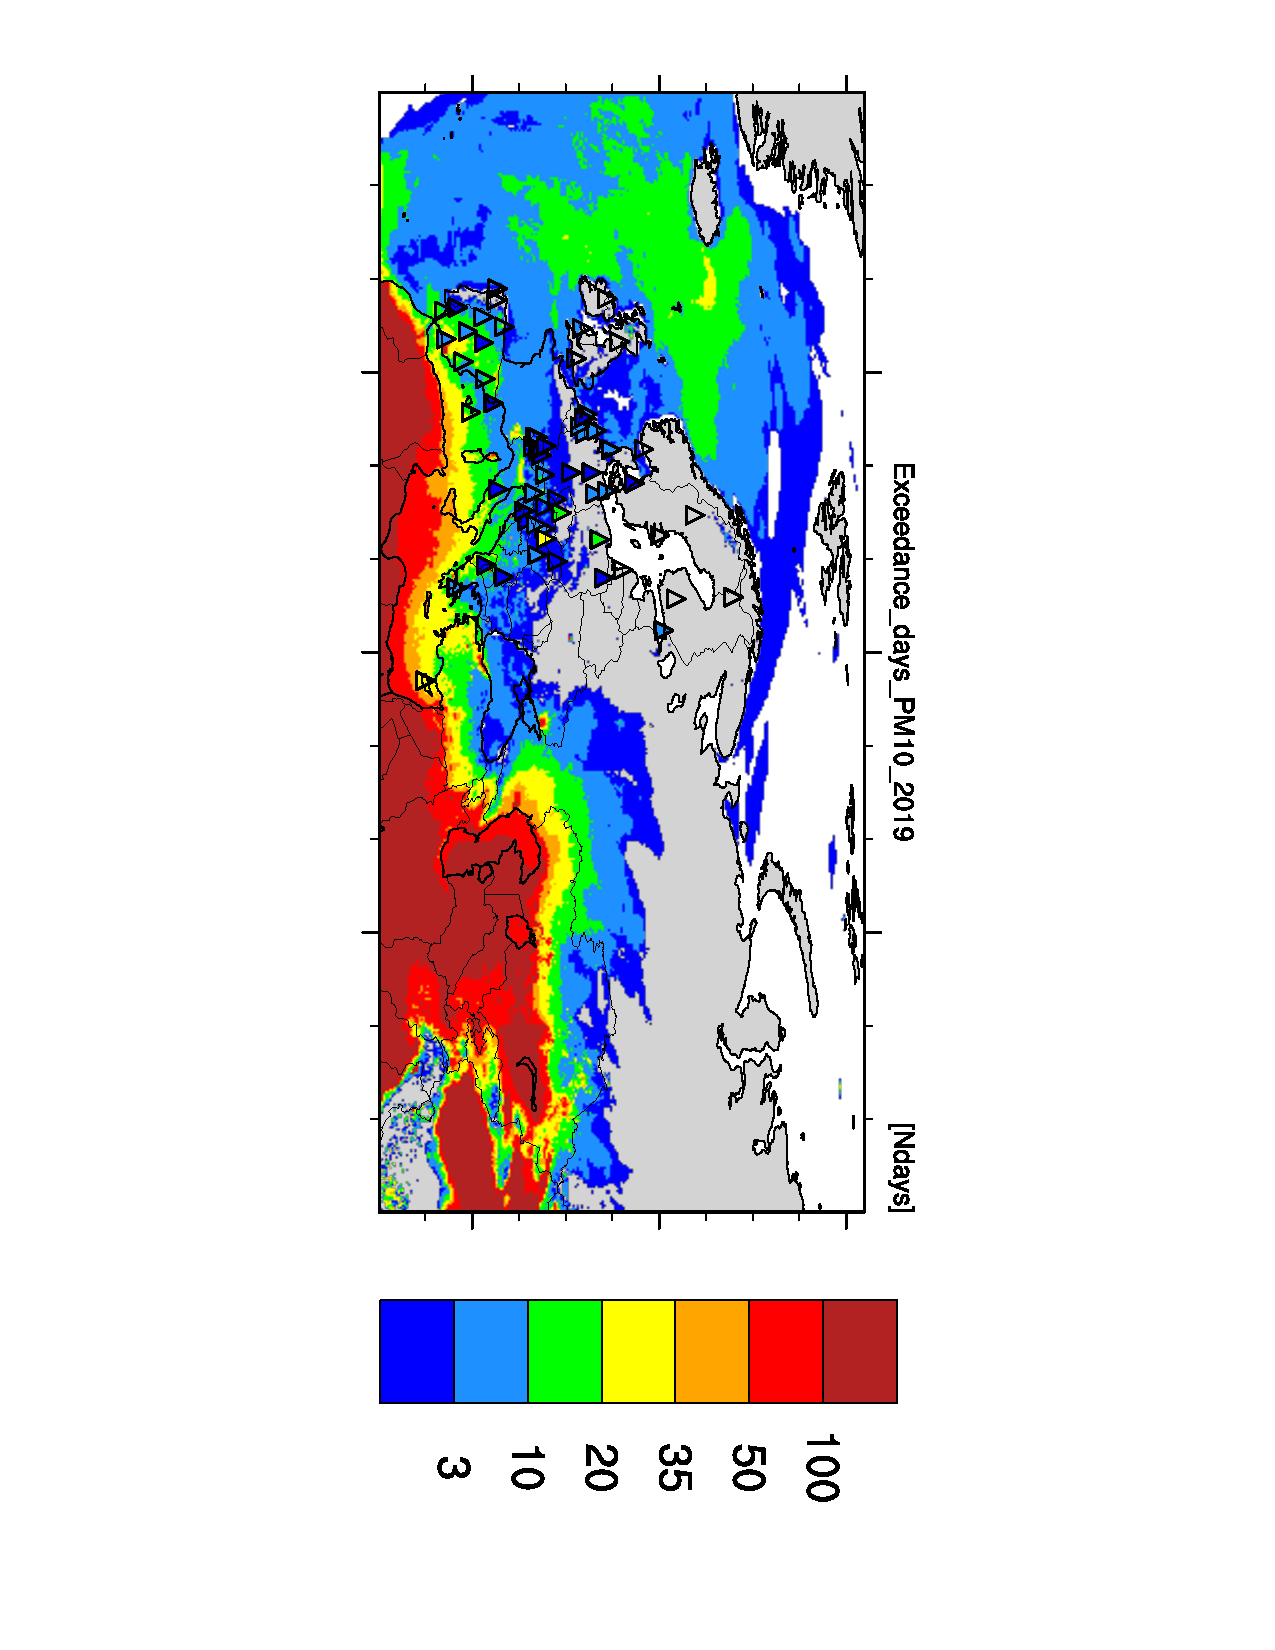
\includegraphics[clip=,angle=90,height=5.9cm,viewport=180 67 440 754]{FIGS_PM/ExcDays_PM10_ModObs_EMEP01_2019.pdf}}\\
  \vspace{0.5cm}
  \centering{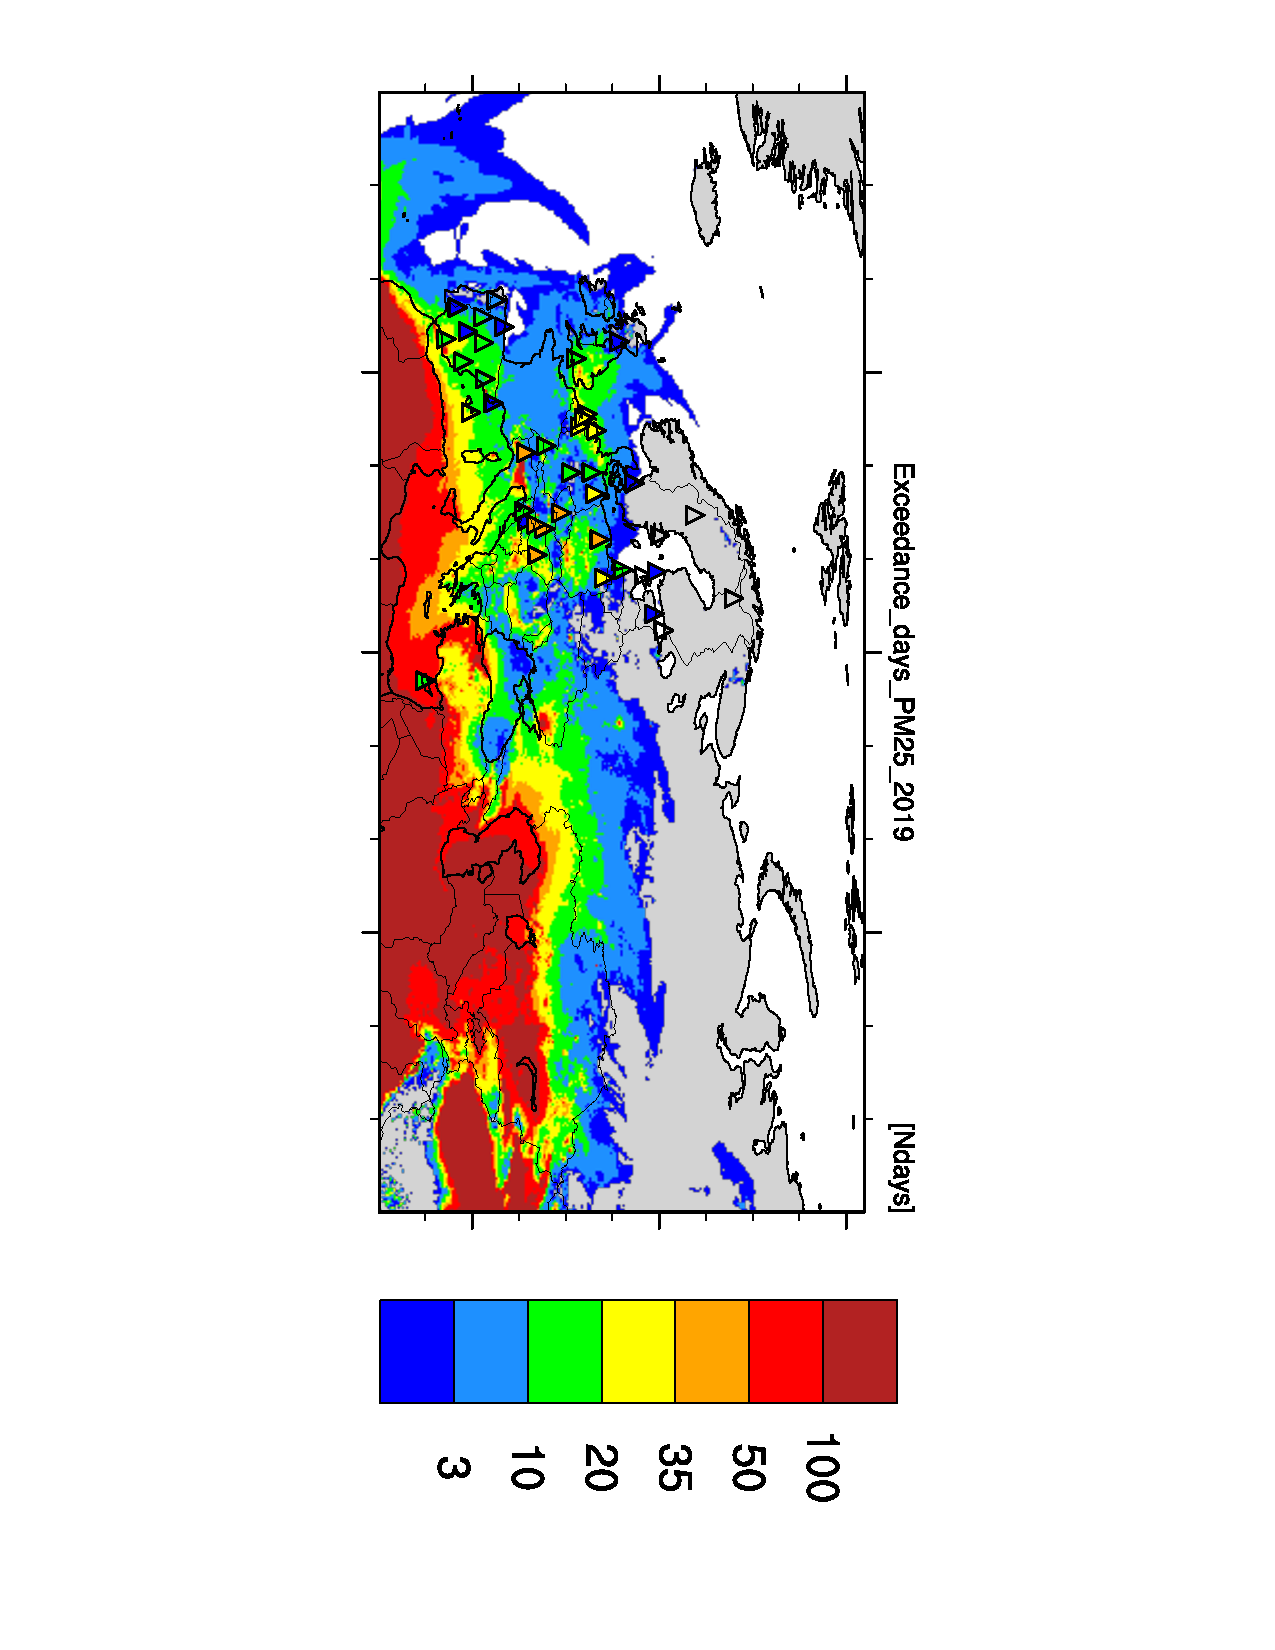
\includegraphics[clip=,angle=90,height=5.9cm,viewport=180 67 440 754]{FIGS_PM/ExcDays_PM25_ModObs_EMEP01_2019.pdf}}
\caption{Calculated (with 0.1\degrees resolution) and observed (triangles) number of days with
  exceedances in 2019: \PM[10] exceeding 50 \ug (upper) and \PM[2.5]
  exceeding 25 \ug (lower panel). \textit{Note: The EU Directive requires no
    more than 35 days with exceedances for \PM[10], whereas WHO
    recommends no more than 3 days with exceedances for \PM[10] and
    \PM[2.5] per calendar year. }}
\label{fig:PMexceed}
\end{figure}


The maps in Figure~\ref{fig:PMexceed} show the number of days with
exceedances of 50 \ug for \PM[10] and 25 \ug for \PM[2.5] in 2019:
modelled values as colour contours and observed values as triangles.

Out of the 67 sites with daily or hourly \PM[10] measurements with data
coverage above 75\%, exceedance days were observed at 31 sites. No
violations of the \PM[10] EU limit value (more than 35 exceedance
days) were observed. Still, 12 sites had more than 3 exceedance days, as rocommended by the WHO AQG. The highest numbers of days
with observed exceedances of \PM[10] were 7 at DE0001 and 6 at LV0010 and RS0005.

\PM[2.5] concentrations exceeded the WHO AQG recommended limit of 25 \ug at 37 out of 51
stations in 2019. Among those, at 21 sites the number of exceedance
days were more than 3 (the recommended limit according to WHO AQG). 
The highest number of exceedance days was 40, observed at HU0002 and IT0004, followed by 30, 26 and 24 exceedance days at DE0044, PL0005 and AT0002, respectively.

The modelled number of exceedance days for 2019 shows in general a good correspondence with the observations, with somewhat better agreement for \PM[10] than for \PM[2.5]. For \PM[10], the model happens to underestimate the occurrence of exceedances of the EU limit value of 50 \ug for some central European sites, for instance for AT0002 and the Dutch sites NL0009 and NL0010 (no modelled exceedance days versus 5 observed), and in the Baltic for LV0010 (0 exceedance day vs. 6 observed). On the other hand, the model tends to overestimate the number of exceedance days at some Mediterranean sites, influenced by Saharan dust, e.g. at the Cypriot site CY0002 (21 vs. 4 observed) and several Spanish sites (in particular ES0007 with 21 vs. 2 observed). Most of the exceedances registered at the Central European sites occurred during the winter (mainly caused by residential combustion) and in the spring (often due to agricultural emissions), while rather few exceedances occurred in the autumn 2019, which was rather wet. By contrast, at the Mediterranean sites the exceedances were more frequent during summer.

For \PM[2.5], the model reproduces number of exceedance days at IT0004 (40), with most of then (61 \%) coinciding with the observed ones. However, it calculates 12 exceedance days versus 40 observed at HU0002, only 3 versus 30 observed at DE0044, and no exceedance days versus 26 observed at PL0005. At the Dutch sites, the model slightly underestimates observed \PM[2.5] exceedance days at NL0009 and NL0010, but overestimates those at NL0091 and NL0644 (same as for 2018 reported last year). Similar to \PM[10], the model calculates a larger number of exceedance days for \PM[2.5] compared with observations at CY0002 (47 vs 3 observed) and several Spanish sites, which is related to the uncertainties in windblown dust modelling. The seasonality of \PM[2.5] exceedances is similar to that of \PM[10], with most exceedance days at the Mediterranean sites in summer and at the other sites in winter, spring and autumn. The only difference is that the largest number of \PM[2.5] exceedances at three of four German sites occurred in spring, while much fewer occurred during the cold seasons. As discussed above, much rain in November-December combined with the mild winter temperatures resulted in the absence of major PM episodes in 2019 typical for Europe in winters.

\vspace{5cm}

%\clearpage
\subsection{Deposition of sulfur and nitrogen} %Hilde to rewrite. Anna to update figures. Done, some final checks on numbers are necessary
\label{subs:dep}


\begin{figure}[H]
  \centering
  \subfigure[oxidized S] {\includegraphics*[viewport=187 62 415 750,clip,angle=90,scale=0.60]{FIGS_STATUS/Mean_in_2019_DEP_SOX_EMEP01.pdf}}
  \subfigure[oxidized N] {\includegraphics*[viewport=187 62 415 750,clip,angle=90,scale=0.60]{FIGS_STATUS/Mean_in_2019_DEP_OXN_EMEP01.pdf}}
  \subfigure[Reduced N] {\includegraphics*[viewport=187 62 415 750,clip,angle=90,scale=0.60]{FIGS_STATUS/Mean_in_2019_DEP_RDN_EMEP01.pdf}} 
 \caption{Deposition of sulfur and nitrogen [mg(S)m$^{-2}$, mg(N)m$^{-2}$] in 2019.}
\label{deps}
\end{figure}

Modelled total depositions of sulfur and oxidised and reduced nitrogen are presented in Figure \ref{deps}.
For sulfur, many hot spots are found in the south-eastern part of the domain. In addition, volcanic emissions of SO$_2$ lead to high depositions in and around Sicily.

Oxidised nitrogen depositions are highest in northern Germany, the Netherlands, Belgium, Poland and northern Italy. These countries also have high depositions of reduced nitrogen, as do parts of the United Kingdom, France and Belgium in western Europe, and Turkey, Georgia, Armenia, Azerbaijan, Kyrgyzstan, Uzbekistan and Tajikistan in the east. 

In Figure \ref{wdeps} wet depositions of nitrogen and sulfur compounds are compared to measurements at EMEP sites for 2019. Overall, the bias of the model with respect to measurements is around 
-32\% to +19\% (Appendix~\ref{ch:appx_modeleval}), but higher for individual sites. A more detailed comparison between model and measurements for the year 2019 can be found at \url{https://aeroval.met.no/evaluation.php?project=emep&exp_name=2021-reporting}.

\begin{figure}[H]
  \centering
  \subfigure[oxidized S] {\includegraphics*[viewport=187 62 415 750,clip,angle=90,scale=0.60]{FIGS_STATUS/so4wdep_2019_ModObs_EMEP01.pdf}}
  \subfigure[oxidized N] {\includegraphics*[viewport=187 62 415 750,clip,angle=90,scale=0.60]{FIGS_STATUS/no3wdep_2019_ModObs_EMEP01.pdf}}
   \subfigure[Reduced N] {\includegraphics*[viewport=187 62 415 750,clip,angle=90,scale=0.60]{FIGS_STATUS/nhxwdep_2019_ModObs_EMEP01.pdf}} 
 \caption{Modelled wet deposition of sulfur and nitrogen [mg(S)m$^{-2}$, mg(N)m$^{-2}$] in 2019, with EMEP observations on top (marked by triangles).}
\label{wdeps}
\end{figure}

\clearpage
\bibliographystyle{copernicus}         % change bibliography-name after each
\renewcommand\bibname{References}      % bibliographystyle command!
\addcontentsline{toc}{section}{References}
\bibliography{Refs2021}
 
%TMP\chapter[Emissions 2019]{Emissions for 2019}
\label{ch:emis2019}


{\bf{Bradley Matthews, Katarina Mareckova, Sabine Schindlbacher, Bernhard Ullrich, \\
Robert Wankm\"uller and all CEIP/Umweltbundesamt Austria, Jeroen Kuenen (TNO)}}
\vspace{30pt}

In addition to meteorological variability, changes in the emissions
affect the inter-annual variability and trends of air pollution,
deposition and transboundary transport.  
The main changes in emissions in 2019 with respect to previous years
are documented in the following sections.


The EMEP Reporting guidelines \citep{UNECE2014} requests all Parties
to the LRTAP Convention to report annually emissions of air pollutants
(\sox\footnote{``Sulphur oxides (\sox)'' means all sulphur compounds,
  expressed as sulphur dioxide (\soii), including sulphur trioxide
  (\soiii), sulphuric acid (\sulacid), and reduced sulphur compounds,
  such as hydrogen sulphide (H${_2}$S), mercaptans and dimethyl
  sulphides, etc.}, \noii\footnote{``Nitrogen oxides (\nox)'' means
  nitric oxide and nitrogen dioxide, expressed as nitrogen dioxide
  (\noii).}, CO, NMVOCs\footnote{``Non-methane volatile organic
  compounds'' (NMVOCs) means all organic compounds of an anthropogenic
  nature, other than methane, that are capable of producing
  photochemical oxidants by reaction with nitrogen oxides in the
  presence of sunlight.}, \nhiii, HMs, POPs,
PM\footnote{``Particulate matter'' (PM) is an air pollutant
  consisting of a mixture of particles suspended in the air. These
  particles differ in their physical properties (such as size and
  shape) and chemical composition. Particulate matter refers to:\\  
(i) ``PM$_{2.5}$'', or particles with an aerodynamic diameter equal to or
  less than 2.5 micrometers ($\mu$m);\\ 
(ii) ``PM$_{10}$'', or particles with an aerodynamic diameter equal to or
  less than 10 $\mu$m.} and voluntary BC) and associated activity data. Projection data, gridded data and information on large point sources (LPS) 
have to be reported to the EMEP Centre on Emission Inventories and Projections (CEIP) every four years.

\section{Reporting of emission inventories in 2021}

Completeness and consistency of submitted data have improved significantly since EMEP started collecting information on emissions. Data of at least 47 Parties each year were submitted to CEIP since 2017 (see Figure~\ref{fig:CEIP1}). In 2021 (as of 1 June 2021), 48 Parties (94\%) submitted inventories\footnote{The original submissions from the Parties can be accessed via the CEIP homepage on \url{https://www.ceip.at/status-of-reporting-and-review-results/2021-submissions}.}, three Parties\footnote{Azerbaijan, Bosnia and Herzegovina and Kyrgyzstan} did not submit any data and 42 Parties reported black carbon (BC) emissions (see section~\ref{sec:bc}). As 2021 is a reporting year for large point sources (LPS) and gridded emissions, 32 Parties reported information on LPS, 26 Parties reported gridded data  \citep{CEIP2021}.

\begin{figure}[h]
\centering
{\includegraphics*[viewport=60 295 550 500,clip,scale=0.75]{FIGS_CEIP/Fig1.pdf}}
\caption{Parties reporting emission data to EMEP since 2002, as of 1 June 2021.}
\label{fig:CEIP1}
\end{figure}

The quality of the submitted data across countries differs quite significantly. By compiling the inventories, countries have to use the newest available version of the {\it EMEP/EEA air pollutant emission inventory guidebook}, which is the version of 2019 \citep{EmisInvGuide2019}. However, many countries still use the 2016 Guidebook \citep{EmisInvGuide2016} or older versions (e.g. \cite{EmisInvGuide2013}). As analysed in a technical report \citep{CEIP2021b}, uncertainty of the reported data (national totals, sectoral data) is relatively high, e.g. the reported uncertainty estimates ranged from 6.9\% to 56\% for \nox emissions reported in 2020. Further, the completeness of reported data has not turned out satisfactory for all pollutants and sectors either.

More detailed information on recalculations, completeness and key
categories, plus additional review findings can be found in the annual
CEIP technical country  reports{\footnote{\url{https://www.ceip.at/review-of-emission-inventories/technical-review-reports}}}.

Indeed, the issue of recalculations is highly relevant to users of EMEP emissions datasets. The aforementioned CEIP report on uncertainties in reported emissions highlighted how time series of reported emissions can vary significantly over subsequent rounds of submissions due to inter alia revisions in activity data, updates of methods and emissions factors and/or inclusion of previously overlooked sources of emissions \citep{CEIP2021b}.
%As an indication of potential revisions in reported emissions,  Appendix 1 lists the EMEP country emissions where emissions for the year 2019 (reported in 2021) deviate from respective emissions for the year 2018 (reported in 2020) by more than 10\%. This Appendix furthermore indicates whether these reported emissions times have been included in the EMEP datasets for modellers, or whether they have been partially or completely replaced during the quality assessment and gap-filling procedure.}
The following subchapters summarise the inventory submissions in terms of three topics that are currently of high interest within the Convention:

\begin{itemize}
\item Reporting of black carbon emissions (\ref{sec:bc})
\item Inclusion of the condensable component in particulate matter emissions (\ref{sec:EmisSVOC}) 
\item Comparison of reported Party emissions to respective reduction targets set out in the Gothenburg Protocol  (\ref{sec:GP})
\end{itemize}
  
%\subsection{Black Carbon (BC) emissions}
\section{Black Carbon (BC) emissions}  
\label{sec:bc}

Over the last decade, black carbon (BC) has emerged as an important air pollutant in terms of both climate change and air quality.  

\begin{figure}[h]
\centering
%{\includegraphics*[viewport=30 260 585 525,clip,scale=0.7]{FIGS_CEIP/Fig2.pdf}}
{\includegraphics*[viewport=1 1 950 465,clip,scale=0.4]{FIGS_CEIP/Fig2.pdf}}
\caption{Black carbon emissions of the year 2019 as reported by CLRTAP Parties.}
\label{fig:CEIP2}
\end{figure}


The emerging significance of BC is mirrored in developments in the international policy arena with respect to emissions reporting.
Since the Executive Body Decision 2013/04, Parties to the LRTAP Convention have been formally encouraged to
submit inventory estimates of their national BC emissions, and in 2015 the reporting templates were updated to include
BC data emissions.

%% In addition to reporting under CLRTAP, EU member states are also encouraged to submit BC emissions
%% estimates as part of their emissions reporting under the National Emissions Ceilings (NEC) Directive (2016/2284/EU).


While BC is not a mandatory pollutant to be reported under the Convention, CEIP continues to monitor and review the level of BC reporting by the Convention's Parties. A brief overview of BC emissions estimates submitted by Parties in 2021 is given below.  %Figure~\ref{fig:CEIP2} 

Since enabling the reporting of BC, a total of 45 CLRTAP Parties have reported BC emissions estimates\footnote{ As of 1 June 2021  Austria, Bosnia and Herzegovina, Liechtenstein, Luxembourg, Russia, and Turkey have yet to report estimates of national BC emissions.}. In this round of reporting, 30 CLRTAP Parties submitted a complete time series of national total BC emissions (1990-2019), while 38 CLRTAP Parties submitted a complete time series from 2000 onwards. Furthermore, 42 EMEP Parties have provided national total BC emissions estimates for the year 2019 (see Figure~\ref{fig:CEIP2}).

For more detailed information on BC consult the annual CEIP technical inventory review report \citep{CEIP2020}.


\section{Inclusion of the condensable component in reported PM emissions}
\label{sec:EmisSVOC}

The condensable component of particulate matter is a class of organic compounds of low volatility that may exist in equilibrium between the gas and particle phase. It is probably the biggest single source of uncertainty in PM emissions. For more background see \citet{CONDws2020}.
%% The condensable component of particulate matter is released as a gas but forms particles when it is diluted and cools
%% down.
Currently the condensable component is not included or excluded consistently in PM emissions reported by Parties
of the LRTAP Convention. Also in the EMEP/EEA Guidebook \citep{EmisInvGuide2019} the condensable fraction is not consistently included or
excluded in the emission factors. Various EMEP centres and task forces and other stakeholders jointly discuss the topic and work on progress in this area. An important activity in 2020 was the workshop organised by MSC-W that resulted in a workshop report \citep{CONDws2020}. However, at the moment PM emissions reported by Parties to the LRTAP Convention are not directly
comparable, which has implications on the modeling of overall exposure to PM.

Small scale combustion sources make a notable contribution to total PM emissions. For all Parties that reported PM$_{2.5}$ emissions for ''1A4bi Residential: Stationar'' for the year 2019 the average contribution to the national total PM$_{2.5}$ emissions from this source category was 46\%. Small-scale combustion is one of the sources where the inclusion of the condensable component has the largest impact on the emission factor. For example, for conventional woodstoves, one of the most important categories in Europe, the emission factors excluding and including the condensable fractions may differ by up to a factor of five \citep{DeniervanderGon2015}.
To improve the quality of the input data for air quality models, and following a decision of \citet{EMEPBureaux2020}, the group of experts that met at the workshop organised by MSC-W agreed on the following approach (for more details see \citet{CONDws2020}): 

\begin{itemize}
\item In year one (2020) the so-called REF2 emission data provided by TNO, which include condensable organics,  is used in an initial estimate for residential combustion emissions. The REF2 data and their usage in the EMEP modeling work in 2020 are described  in  \citet{R2020:CAMSREF2} and \citet{R2020:SVOC}. 
\item  In subsequent years these top-down estimates should be increasingly replaced by national estimates once procedures for quantifying condensables in a more harmonized way are agreed on and implemented.
\end{itemize}

CEIP in co-operation with TNO prepared a list of Parties where it could be assumed with a good degree of certainty that the condensable component is mostly included in PM emissions for GNFR sector C. The analysis focused on small scale combustion. This analysis was based on (a) the calculation of Implied Emission Factors (emission divided by the reported activity data), (b) the fuel mix of the Party, (c) the information provided in the Informative Inventory Report and (d) in a few cases direct information from Parties (received via e-mail).

The analysis resulted in a list of Parties where the conclusion was that the PM emission data reported by the Party should be used as the condensable component seemed to be included. For other Parties the TNO REF2 data were used. In a few cases data that had been gap-filled by CEIP was used as for the respective Party no REF2 estimate was available (see table~\ref{tab:CEIP1}).



\begin{table}
  \caption{Data source for PM emission in GNFR C used in EMEP modelling in 2021.}
\centering
{\includegraphics*[viewport=120 275 550 760,clip,width=0.8\textwidth]{FIGS_CEIP/Table1.pdf}}
\label{tab:CEIP1}  
\end{table}

Parties were asked to include a table with information on the inclusion of the condensable component in PM$_{10}$ and PM$_{2.5}$ emission factors for reporting under the CLRTAP Convention in 2021. This table has been added to the revised
recommended structure for IIRs\footnote{\url{https://www.ceip.at/reporting-instructions } }. Twenty-three Parties provided information on the inclusion of the condensable component in PM$_{10}$ and PM$_{2.5}$ emission factors\footnote{Status as of 15 May 2021}. This reporting is a first step towards a better understanding of reported PM data. The information that Parties provided on whether the condensable component is included in PM emissions was quite heterogeneous. The status of inclusion or exclusion is best known for emissions from the energy sector and road transport, for which many Parties submitted information. 

\subsection{REF2 emissions and improvements compared to last year}


The REF2 emission inventory provides a bottom-up database of PM emissions (both PM$_{10}$ and PM$_{2.5}$) from small combustion activities (GNFR category C), taking into account activity data and consistent emission factors that include condensables, for both wood and solid fuel combustion. It was originally developed for the year 2010 \citep{DeniervanderGon2015}. Residential emissions vary from year to year, because of technological developments in the sector (replacement of stoves and boilers) but also because of the heating demand due to fluctuating temperatures. To take this into account, an alternative REF2 was developed for 2015 which was also used as an input to EMEP modelling in 2020. These REF2 emission data and their usage in the EMEP modelling work in 2020 are described in  \citet{R2020:CAMSREF2} and \citet{R2020:SVOC}. This version was developed by scaling the original REF2 for 2010 to the year 2015 by using the trend in the official reported data for PM$_{2.5}$ from GNFR~C for that particular year. The idea behind this approach was that by scaling in this way both the technological changes within each country as well as the annual fluctuation in heating demand are included. It is desirable but difficult to separate these effects because the detailed underlying country data are not available. Countries report emissions only by source sector and for the sum of all fuels; activity data or emissions by appliance type are not available.

This scaled REF2 for the year 2015 has been used both in EMEP and other modelling activities, and presented in various international expert group meetings such as CAMS, EMEP and UNECE Task Forces (in particular TFEIP and TFMM). This triggered several discussions with experts (including some specific countries), which resulted in the provision of additional information of the national circumstances on the types of stoves installed, etc. (see also \cite{CONDws2020}). 

With this information, as well as additional information made available by IIASA (Z. Klimont), for 5 specific countries (Austria, Germany, Finland, France, the Netherlands) the REF2 emission estimates were revised. The main reason to change the emission estimates is the new information that became available on the appliance types, especially regarding the split between different types of heating stoves (traditional vs. modern). For modern stoves, the PM emission factors are significantly lower compared to traditional stoves, and for the condensable component of PM this effect is even larger.
The 5 selected countries were chosen because of feedback received or discussions with national experts which suggested that REF2 emissions may be overestimating. It is planned to also revisit the REF2 emission estimates for the other countries, but this is ongoing work.

\begin{figure}[h]
\centering
{\includegraphics*[viewport=1 1 740 400,clip,scale=0.45]{FIGS_CEIP/Fig3.pdf}}
\caption{Results for REF2 for 2010 (original), 2015 (after scaling, used in EMEP 2020) and 2015 (after scaling + adjustment for 5 countries, used in EMEP 2021).}
\label{fig:CEIP3}
\end{figure}


Figure~\ref{fig:CEIP3} shows the different REF2 emission estimates. The year 2010 is the original REF2 estimate, while 2015\_scaled represents the scaled REF2 (REF2.1) to the year 2015 using the official reported data (used in the 2020 EMEP modelling). The estimate 2015\_scaled\_adjusted is the updated version described here, where for 5 selected countries the REF2 data have been revised based on new information.
From the figure, it can be seen that the 2015 emission is lower than 2010 for almost all countries. This is partly the result of technological advancements in countries (replacement of older stoves with new ones), but also largely related to the fact that 2010 was a relatively cold year in Europe, hence with higher emissions from the residential sector compared to other years. The figure also shows that for the five countries that have been adjusted in the latest update, in each case the REF2.1 emission including condensables is corrected downward. This adjusted REF2.1 is, however, still considerably higher than reported emission for each of these countries.

\section{Gothenburg Protocol targets}
\label{sec:GP}

The 1999 Gothenburg Protocol (GP) lists emission reduction commitments of  \nox,
\sox, NMVOCs and \nhiii for most of the Parties to the LRTAP Convention for the year 2010 (\cite{UNECE1999}). These commitments should not be exceeded in 2010 and in subsequent years either.

In 2012, the Executive Body of the LRTAP Convention decided that adjustments to inventories may be applied in some circumstances (\cite{UNECE2012}). From 2014 to 2021, adjustment applications of ten countries (Belgium, Czechia, Denmark, Finland, France, Hungary, Germany, the Netherlands, Luxembourg, Spain and the United Kingdom) have been accepted by expert review team and therefore these approved adjustments have to be subtracted for the respective countries when compared with the targets. In April 2021, Czechia and France  submitted  new adjustment applications; the \nhiii adjustment application  of Czechia was rejected by the review team and application from France has been accepted.     

Further, the reporting guidelines (\cite{UNECE2014}) specify that some Parties within the EMEP region (i.e. Austria, Belgium, Ireland, Lithuania, Luxembourg, the Netherlands, Switzerland, the United Kingdom of Great Britain and Northern Ireland) {\it may choose to use the national emission total calculated on the basis of fuels used} in the geographic area of the Party as a basis for compliance with their respective emission ceilings.

However, when considering only reported data, approved adjustments and fuel used data of the respective countries, Figure~\ref{fig:CEIP4} indicates that in the year 2019 North Macedonia could not reduce their \sox emissions below their respective Gothenburg Protocol requirements, and that Croatia and Spain are above their 1999 Gothenburg Protocol ceilings concerning \nhiii. For \nox and NMVOC all countries were below their individual ceilings in year 2019.


\begin{figure}[h]
\centering
{\includegraphics*[viewport=1 1 753 323,clip,scale=0.55]{FIGS_CEIP/Fig4.pdf}}
\caption{Distance to Gothenburg Protocol targets in 2019 (based on reported data in 2021).
  Only Parties that ratified the Gothenburg Protocol are included. 
  * Emission data based on fuels used for road transport.
Approved adjustments are considered for  Denmark (NMVOCs, \nhiii), Finland (\nhiii),  Germany (\nox, NMVOCs, \nhiii), Luxembourg (\nox, NMVOCs), the Netherlands (\nhiii, NMVOCs).}
\label{fig:CEIP4}
\end{figure}





\section{Datasets for modellers 2021}
\label{sec:modeldata}

Under the Convention, CEIP is responsible for synthesizing the reported emissions data of the EMEP countries into complete gridded emissions datasets for the EMEP domain (covering the geographic area between 30\degrees N-82\degrees N latitude and 30\degrees W-90\degrees E longitude. These data are mainly used for modelling of air pollutant concentrations and depositions.

To compile these datasets each year, CEIP synthesizes and evaluates the most recent national sectoral emissions estimates and national gridded emissions data reported by the EMEP countries. CEIP strives to include, to the largest possible extent, the reported emissions data it receives from EMEP countries. However, due to cases of non-reporting or identified quality issues in the reported data, emissions need to be gap-filled or replaced. Furthermore, it should be noted how gridded and sectoral emissions totals are combined in compiling these datasets. National gridded emissions data, even if reported annually, are not directly utilized but are rather used to map out relative emissions, with which national sector emission totals are spatially distributed. Of course if for a given year both national sector emissions totals and gridded estimates reported by a given country pass through the CEIP QA/QC checks, the generated gridded emissions will be identical to the gridded emissions reported by the country.
The following subchapters describe important aspects of the 2021 EMEP datasets, summarising:

\begin{itemize}
    \item The status of reporting of national gridded emissions data and the extent to which these are used to distribute emissions spatially (Section~\ref{sec:griddedemis})
    \item The extent to which sectoral emissions were gap-filled or replaced (Section~\ref{sec:gapfilling})
    \item  The sectoral contributions (Section~\ref{sec:GNFRsec}) and temporal trends (Section~\ref{sec:emistrends}) in the emissions of carbon monoxide, nitrogen oxides, sulphur oxides, ammonia, non-methane volatile organic carbons, and particulate matter including black carbon. Trends in shipping emissions are discussed separately (Section~\ref{sec:shiptrends}).     
\end{itemize}


\subsection{Reporting of gridded data}
\label{sec:griddedemis}

\begin{table} 
  \caption{Gridded emissions in 0.1{\degrees}$\times$0.1{\degrees} longitude/latitude resolution reported until 2017, 2020 and 2021.}
%\vspace{15pt}
\centering
{\includegraphics*[viewport=115 65 550 740 ,clip,width=0.95\textwidth]{FIGS_CEIP/Table2.pdf}}
\label{tab:emis01degreported}  
\end{table}


After the first round of submissions in 2017, 2021 was the second year for which EMEP countries were obliged to report gridded emissions in the grid resolution of 0.1{\degrees}$\times$0.1{\degrees} lon\-gi\-tude/la\-ti\-tude. As of June 2021, 34 of the 48 countries which are considered to be part of the EMEP area reported sectoral gridded emissions in this resolution.


The majority of gridded sectoral emissions in 0.1{\degrees}$\times$0.1{\degrees} lon\-gi\-tude/la\-ti\-tude resolution have been reported for the year 2015 (32 countries). For 2019 gridded sectoral emissions have been reported by 29 countries, for 2016, 2017 by five countries and for 2018 by four countries. Comparing to reporting in 2017, reported gridded data are available for 11 more countries in 2021.

Fifteen countries reported gridded emissions additionally for previous years (one country for the whole time series from 1980 to 2019; one country for the whole time series from 1990 to 2019; seven countries for the years 1990, 1995, 2000, 2005 and 2010; one country for the years 1990, 2000, 2005 and 2010; one country for the years 2000, 2005 and 2010; one country for the year 2005; one country for the year 2010; and two countries for the year 2014).


Reported gridded sectoral data in 0.1{\degrees}$\times$0.1{{\degrees}} lon\-gi\-tude/la\-ti\-tude resolution, which can be used for the preparation of gridded emissions for modelers, covers less than 25\% of the cells within the geographic EMEP area. For the remaining areas (or for EMEP countries that have no reported gridded data) missing emissions are gap-filled and spatially distributed by expert estimates. Reported grid data can be downloaded from the CEIP website\footnote{\url{https://www.ceip.at/status-of-reporting-and-review-results}}. The gap-filled gridded emissions are also available there\footnote{\url{https://www.ceip.at/webdab-emission-database/emissions-as-used-in-emep-models}}. 

An overview of gridded data in 0.1{\degrees}$\times$0.1{{\degrees}} lon\-gi\-tude/la\-ti\-tude resolution reported in 2017, 2020 and 2021 is provided in Table~\ref{tab:emis01degreported}.

%while an example map of the gap-filled and gridded \nox emissions in 2018 in 0.1{\degrees}$\times$0.1{\degrees} longitude-latitude resolution is shown in Figure~\ref{fig:CEIP5}.


%% \begin{figure}[h]
%% \centering
%% {\includegraphics*[viewport=25 200 585 585,clip,scale=0.7]{FIGS_CEIP/Fig5.pdf}}
%% \caption{Visualized gap-filled and gridded \nox emissions in 0.1{\degrees}$\times$0.1{\degrees} long-lat resolution.
%% }
%% \label{fig:CEIP5}
%% \end{figure}


For compiling the 2021 EMEP emisisons dataset, reported gridded data in 0.1{\degrees}$\times$0.1{\degrees} longitude-latitude resolution was used from Austria, Belgium, Bulgaria, Croatia, Cyprus, Czechia, Denmark, Estonia, Finland, France, Georgia, Germany, Greece, Hungary, Ireland, Latvia, Luxembourg, Malta, Monaco, Netherlands, North Macedonia, Norway, Poland, Portugal, Romania, Slovakia, Slovenia, Spain, Sweden, Switzerland and United Kingdom.


\subsection{Gap-filling of reported data in 2021}
\label{sec:gapfilling}

As described above, sectoral emissions reported by the EMEP countries are used, to the largest extent possible, to compile the gridded EMEP datasets. Each year the reported source-sector level data of the (NFR level) are aggregated into the 13 GNFR sectors and are then evaluated to identify countries for which emissions have not been reported or appear to exhibit implausible emission levels and/or trends. Based on this assessment, a procedure is then implemented to gap-fill missing emissions data and to replace data that have been identified as implausible. The sectoral emissions are then distributed spatially using, where available (and appropriate), the reported national gridded emissions as relative spatial proxies, or other independent datasets of spatial proxies.

Given the end of May deadline for compiling EMEP datasets, a cut-off date for incorporating reported emissions has to be set to allow necessary time for evaluating the reported emissions and implementing the gap-filling procedure. This year, the sectoral emissions data reported by 14 April 2021 were evaluated and considered for use in the compilation of the 2021 EMEP datasets of gridded emissions.

The Parties, where data were (partly) replaced, corrected or gap-filled in 2021 are Albania, Armenia, Austria, Azerbaijan, Belarus, Bosnia and Herzegovina, Cyprus, Denmark, Georgia, Kazakhstan, Kyrgyzstan, Liechtenstein, Lithuania, Luxembourg,  Montenegro, the Republic of Moldova, Montenegro, the Russian Federation, Serbia, Turkey and the Ukraine. The results of the quality control and gap-filling procedures are described in detail in CEIP gap-filling report \citep{CEIP2021c}. % and in Appendix 2, a table is provided that documents for which EMEP countries and specific pollutants gap-filling/replacement was required and which methods were implemented. The reader is nonetheless reminded that this Table does not indicate if a subsequent adjustment of reported PM emissions for GNFR Sector C was undertaken to account for the potentially missing condensable component. This information is provided in Table 1.

Finally, it should be noted that the gap-filling and replacement procedure has been updated since 2020. The gap-filling/replacement of EMEP country emissions remains based on the independent estimates from the ECLIPSE v6b\footnote{\url{https://iiasa.ac.at/web/home/research/researchPrograms/air/ECLIPSEv6.html}} dataset that has been compiled by IIASA using their GAINS model \citep{Amann_et_al:2011}. However, the emissions for areas North Africa, remaining Asian areas, the Aral Lake and the part of Russia within the EMEP domain for which Russia does not report emissions (referred to as 'Russian Federation Asian part' further in this chapter), are now based on the updated EDGAR v5.0\footnote{\url{https://edgar.jrc.ec.europa.eu/dataset_ap50}}  dataset \citep{EDGARv50} that was generated by the European Commission's Joint Research Centre (JRC). Previously, the emissions for these areas were based on a previous version (EDGAR v4.3.2) of the dataset \citep{EDGARv432}.


\subsection{Contribution of GNFR sectors to total EMEP emissions}
\label{sec:GNFRsec}

Figure \ref{fig:CEIP6} shows the contribution of each GNFR sector to the
total emissions of individual air pollutants (\sox, \nox, CO, NMVOC,
\nhiii, PM$_{2.5}$, PM$_{10}$, PM$_{coarse}$ and BC).
%To provide a picture as complete as possible of the situation of the individual sectors to total EMEP emissions, data as used for the EMEP models (i.e. gap-filled data) were used for the calculations. 
To clarify, the reader is reminded that these analyses are based on the emission data in the EMEP datasets for modellers i.e. data based largely on reported emissions, but also compiled with independent emissions estimates for countries and regions where data are not reported or the reported data have been omitted due to quality issues. The sea regions were excluded for this sectoral analysis.


\begin{figure}[h]
\centering
{\includegraphics*[viewport=1 1 565 565,clip,width=0.65\linewidth]{FIGS_CEIP/Fig6.pdf}}
\caption{GNFR sector contribution to national total emissions in 2019
  for the EMEP domain apart from the  sea regions.}
\label{fig:CEIP6}
\end{figure}

\begin{figure}[h]
\centering
{\includegraphics*[viewport=1 1 565 565,clip,width=0.65\linewidth]{FIGS_CEIP/Fig7.pdf}}
\caption{GNFR sector contribution to national total emissions in 2019
  for the EMEP West and EMEP East areas. Asian areas, North Africa and the sea regions are not included.}
\label{fig:CEIP7}
\end{figure}

It is evident that the combustion of fossil fuels is responsible for a significant part of all emissions. For \nox emissions, the largest contributions come from transport (sector F, 40\%) and from large power plants (sector A, 21\%).

NMVOC sources are distributed more evenly among the different sectors,
such as 'E - Emissions from solvents' (21\%), 'F - Road transport' (30\%), 'D - Fugitive Emissions' (14\%), 'B - Industry combustion' (7\%), 'K - Manure management' (9\%) and 'C - Other stationary combustion' (12\%).


The main source of  \sox emissions are large point sources from combustion in energy and transformation industries (sector A, 56\% and sector B, 23\%).

Ammonia arises mainly from agricultural activities; about 92\% combined contribution from sectors K and L. Emissions of CO  originate primarily from 'F - Road transport' (51\%) and 'C - Other stationary combustion'  (26\%). 

The main sources of primary PM$_{10}$ and PM$_{2.5}$ emissions  are industry (23\% and 20\%) and other stationary combustion processes (39\% and 55\%). Due to the higher agricultural emissions of PM$_{10}$ versus PM$_{2.5}$, sectors K and L make a much larger relative contribution to PM$_{coarse}$ emissions (29\% combined) together with significant contributions from 'B - industry combustion' (26\%) and 'C - Other stationary combustion' (29\%). 

Finally, the most important contributors to BC emissions are 'F - Road transport' (18\%) and 'C - Other stationary combustion' (57\%).

Figure \ref{fig:CEIP7} illustrates the
sector contributions to the sum of total emissions in the EMEP West
region and the EMEP East region. The split between the EMEP West and EMEP East regions is according to  \url{https://www.ceip.at/countries} (sea regions, North Africa and the remaining Asian areas are excluded, with the Aral Lake area assigned to EMEP East). The comparison of both graphs highlights some significant differences between West and East. 

For \nox in both the EMEP West and EMEP East regions the most important sector is 'F - Road transport emissions' (38\% and 34\%, respectively), although it is worth noting the higher contribution from  'A - Public electricity and heat production'  in the East region (23\%).

For NMVOC in the EMEP West region the most relevant sector is 'E - Emissions from solvents' with a share of 35\%. In the EMEP East region the same sector has a considerable lower share  (14\%), whilst the sector 'F - Road transport' is of high importance (32\%).

The main source of \sox are 'A - Public electricity and heat production'  and and 'B - Industry combustion'. These two sectors together contribute to 78\% and 86\%  of the \sox emissions within the EMEP West and EMEP East areas, respectively.

The main sources of \nhiii emissions for both EMEP West and EMEP East are the
agricultural sectors (K and L) with 93\% and 94\%, respectively.

CO emissions arise mainly from 'F - Road transport emissions' (60\%) in EMEP East. In the EMEP West region the main sector is 'C - Other stationary combustion' (40\%).

For PM$_{2.5}$ and PM$_{10}$ 'C - Other stationary combustion' holds a 
significant share of the total emissions in the EMEP West area (54\% and 37\%), compared to the EMEP East area (18\% and 14\%). For the
EMEP East area sector 'B - Industry combustion' is of higher importance. For PM$_{coarse}$ it is worth mentioning the higher contributions from agriculture in the EMEP East area (44\%). Finally, it is interesting to note the significant contribution to BC emissions in the EMEP East area from fugitive emissions (13\% in EMEP East versus 1\% in EMEP West). 


\subsection{Trends in emissions in the geographic EMEP domain}
\label{sec:emistrends}

\begin{figure}[b]
\centering
{\includegraphics*[viewport=1 1 565 370,clip,width=0.75\linewidth]{FIGS_CEIP/Fig8.pdf}}
\caption{Emission trends 2000--2019 in the geographic EMEP area (emissions from international shipping in the sea regions are excluded)}
\label{fig:CEIP8}
\end{figure}

\begin{figure}
\centering
     \subfigure[EMEP West]{\includegraphics*[viewport=1 1 567 375,clip,width=0.6\linewidth]{FIGS_CEIP/Fig9i.pdf}}\\
     \subfigure[EMEP East]{\includegraphics*[viewport=1 1 567 375,clip,width=0.6\linewidth]{FIGS_CEIP/Fig9ii.pdf}}\\
     \subfigure[Other Land Areas]{\includegraphics*[viewport=1 1 567 375,clip,width=0.6\linewidth]{FIGS_CEIP/Fig9iii.pdf}}     
\caption{Emission trends 2000-2019 in the geographic EMEP domain (emissions from international shipping in the sea regions are excluded) divided into three areas: 'EMEP West' (top), 'EMEP East' (middle) and 'Other Land Areas' (bottom), that include the emissions from North Africa and the remaining Asian areas. }
\label{fig:CEIP9}
\end{figure}

The following trend analyses are based on the emissions data in the EMEP datasets for modellers, i.e. data based largely on reported emissions, but also compiled with independent emissions estimates for countries and regions where data are not reported or the reported data have been omitted due to quality issues.

Excluding shipping emissions in the sea regions (these are summarised in the following subchapter), the trend analyses of total emissions from the non-sea areas in the EMEP domain\footnote{The EMEP domain covers the geographic area between 30{\degrees} N-82{\degrees} N latitude and 30{\degrees} 
  W-90{\degrees} E longitude.} show that emissions of seven of the nine pollutants have decreased overall since 2000 Figure~\ref{fig:CEIP8}). Only the 2019 PM$_{coarse}$  and \nhiii emissions have increased (by 6 and 12\%, respectively) since 2000. The 2019 emissions of \sox are 69\% of the respective 2000 emissions. While the 2019 emissions of CO, NMVOC, \nox, PM$_{2.5}$, PM$_{10}$ and BC are all lower than respective emissions in 2000 (1-10\% lower), it is interesting to note that emissions of these pollutants have been increasing since ca. 2014.

Despite these overall trends, assessment shows that regional emission developments seem to follow strongly different patterns (Figure~\ref{fig:CEIP9}). While emissions of all of the pollutants in the EMEP West countries are clearly decreasing, emissions of all pollutants in the EMEP East countries of the EMEP domain have been somewhat stable (albeit gradually decreasing for most pollutants) over the 2000-2019 period. For the Other Land Areas (North Africa and the remaining Asian areas, emissions are clearly on the rise.

Of course it is not just the emission trends that separate the three land regions. Whereas the emission trends of the EMEP West countries are based to a very large extent on the official national inventories reported to CEIP, the countries within the Other Land Areas within the EMEP domain (North Africa, remaining Asian areas) are not Parties to the Convention and thus are not obliged to report their emissions. For these regions, emissions are based completely on the independent gridded emission estimates of the EDGAR v5.0 dataset \citep{EDGARv50} that was generated by the European Commission's Joint Research Centre (JRC). For the EMEP East region, again not all countries are Parties to the Convention (Turkmenistan, Tajikistan and Uzbekistan) and reported Russian emissions do not cover the region of Russia within the EMEP domain that is ca. east of the Urals. Emissions for the area of the Aral Lake are also not reported by any Convention country. Note that the emissions for the eastern part of Russia and the Aral Lake have also been gap-filled using the independent gridded emission estimates of the EDGAR v5.0 dataset. Finally, it should be noted that many of the emissions time series for the EMEP East countries that are Parties have been partially or fully replaced with independent estimates from the ECLIPSE v6b\footnote{\url{https://iiasa.ac.at/web/home/research/researchPrograms/air/ECLIPSEv6.html}} dataset that has been compiled by IIASA using their GAINS model  \citep{Amann_et_al:2011}.
%An overview of the Parties and pollutants for which replacement and gap-filling was required is given in Appendix 2.


Non-sea emission levels in the geographic EMEP domain for 2019 of the individual countries and areas are compared to 2000 emission levels for each pollutant (see Tables~\ref{tab:CEIP3}-\ref{tab:CEIP3} continued). Again, the reader is reminded that the following trend analyses are based on the emissions data in the EMEP datasets for modellers i.e. data based largely on reported emissions, but also compiled with independent emissions estimates for countries and regions where data are not reported or the reported data have been omitted due to quality issues. Overview tables with reported emission trends for individual countries have been published on the CEIP website\footnote{\url{https://www.ceip.at/webdab-emission-database/reported-emissiondata}}. Detailed information on the sectoral level can also be accessed in WebDab\footnote{\url{https://www.ceip.at/webdab-emission-database/emissions-as-used-in-emep-models} and/or \url{https://www.ceip.at/webdab-emission-database/reported-emissiondata}}.

The assessment of emission levels in individual countries and areas show an increase of emissions in 2019 compared to 2000 emission levels in several countries or areas.


In case of PM emissions, 24 countries/areas have higher PM$_{coarse}$ emissions in 2019 than in 2000, while PM$_{10}$ and PM$_{2.5}$ emissions increased in 17 and 16 countries/areas, respectively. In case of \nox and \sox there are 14  countries/areas, NMVOC 13, \nhiii 18 and CO 12
countries/areas with higher emissions in 2019 than in year 2000. Detailed explanatory information on emission trends for the reporting countries should be provided in the respective informative inventory reports (IIRs). Tables~\ref{tab:CEIP3}-\ref{tab:CEIP3} continued indicates whether the emissions were based completely  (R) or partially (r) on reported data. 

\begin{table}
  \caption{Differences between emissions for 2000 and 2019 (based on gap--filled data as used in EMEP models). Negative values mean that 2019 emissions were lower than 2000 emissions. Red/blue coloured data indicates that 2019 emissions were higher/lower than 2000 emissions. Furthermore, the symbol in parentheses indicate whether the emissions times series are completely based on reported data (R), are partially based on reported data (r), or have been completely replaced/gap-filled (-).}
\centering
{\includegraphics*[viewport=45 100 535 735,clip,width=0.99\textwidth]{FIGS_CEIP/Table3_page1.pdf}}
\label{tab:CEIP3}  
\end{table}

\begin{table}
  \caption*{Table~\ref{tab:CEIP3} continued. Differences between emissions for 2000 and 2019 (based on gap--filled data as used in EMEP models).}
\centering
{\includegraphics*[viewport=45 520 535 735,clip,width=0.99\textwidth]{FIGS_CEIP/Table3_page2.pdf}}
\label{tab:CEIP3contd}  
\end{table}

%% CEIP included again a summary of increase/decrease by pollutant here, which I (Agnes) did not include because it has no additional value
%% whatsoever. All info can be found in the table and the text before. I thought we agreed not to write this part anymore. 

\subsection{Trends in emissions from international shipping}
\label{sec:shiptrends}

International shipping emissions are not reported by Parties. Gridded emissions for the sea regions (European part of the North Atlantic, Baltic Sea, Black Sea, Mediterranean Sea and North Sea) were calculated using the CAMS global shipping dataset \citep{CAMSemis2019} for the years 2000 to 2019 (Figure~\ref{fig:CEIP10}), developed by the Finnish Meteorological Institute (FMI), and provided via ECCAD\footnote{\url{https://eccad.aeris-data.fr}} the dataset {\it CAMS\_GLOB\_SHIP} \citep{ECCAD}.

\begin{figure}[h]
\centering
{\includegraphics*[viewport=1 1 553 230,clip,width=0.75\linewidth]{FIGS_CEIP/Fig10.pdf}}
\caption{International shipping emission trends in the EMEP area, extracted from the CAMS global shipping emission dataset developed by FMI, and provided via ECCAD ({\it CAMS\_GLOB\_SHIP}) in April 2019 (for the years 2000 to 2017) and in November 2019 (for the year 2018). These are the emissions which have been used for the most recent trend calculations with the EMEP model.
}
\label{fig:CEIP10}
\end{figure}


According to FMI the high increase in shipping emissions from 2018 to 2019 is because much more small vessels are using AIS than in previous years, which means that emissions from this small vessels are included in the shipping emissions for 2019, but not in previous years.
Due to the selective implementation of the Sulphur Emission Control Areas (SECAs) on the North Sea and Baltic Sea only, the emission trends differ between those seas and the other seas.



\section{Summary}

This chapter summarises the status of emissions reporting by LRTAP Convention Parties and the extent to which these data have been incorporated into the 2021 EMEP emissions datasets for modellers. The chapter documents the historical improvement in reporting over time, noting the increasing extent of reporting of emissions inventories for the mandatory pollutants and black carbon, as well as increased reporting of gridded emissions in 2021 compared to 2017. Despite these positive trends in terms of reporting, reporting is not yet complete. For some parties, emissions inventories and gridded data are not reported (or are reported late and/or incomplete). There is further room for improvement on the reporting of particulate matter emissions with respect to whether the condensable component has been included in the reported estimates.

The 2021 EMEP emissions datasets for modellers therefore need to be complied carefully and this chapter documents for which countries and pollutants the time series have been based fully or partially on reported inventories and gridded data, and for which countries and regions the datasets have been built using independent emissions data products.

Based on the complied datasets in 2021, it is worth noting that the 2000 to 2019 trends in emissions from the land areas have decreased for most pollutants except for PM$_{coarse}$  and \nhiii. This trend appears to be driven by the trends of the EMEP West countries, for which the time series are based almost completely on reported data. In contrast, EMEP East as whole shows a rather stable trend in terms of emissions (emissions based partially on reported data), with notable emissions increases shown for the 'Other areas' (based completely on independent estimates). International shipping emissions had been shown to be decreasing up to 2018; however, a notable jump in 2018  to 2019 emissions of all pollutants likely stems from a methodological artefact, whereby the number of smaller vessels using AIS systems (on which the CAMS global shipping dataset is based) seems to have increased.

\clearpage
\bibliographystyle{copernicus}         % change bibliography-name after each
\renewcommand\bibname{References}      % bibliographystyle command!
\addcontentsline{toc}{section}{References}
\bibliography{Refs,EMEP_Reports,RefsEmis}
 

\part{Trends in air pollution} 

\chapter[Trends]{Trends in observations and EMEP MSC-W model calculations 2000-2019}
\label{ch:Trends}

{\bf{Wenche Aas, Hilde Fagerli, Karl Espen Yttri, Svetlana Tsyro, Sverre Solberg, David Simpson, Jonas Gliss, Augustin Mortier, Eivind Grøtting Wærsted, Hans Brenna, Anne Hjellbrekke, Jan Griesfeller, Agnes Ny\'{\i}ri, Thomas Scheuschner}}\\



\section{\label{sec:Trends_introduction}Introduction and background}
At its thirty-ninth session (Geneva, 9–13 December 2019), the Executive Body launched the review of the Protocol to Abate Acidification, Eutrophication and Ground-level Ozone (the Gothenburg Protocol) as amended in 2012. In order to assess  the progress made towards achieving the environmental and health objectives of the Protocol, a
list of questions was given to the subsidiary bodies of the Air Convention. Several of these questions were related to the trends of air pollution in Europe. 

In this chapter, we present an assessment of the trends in air pollution in Europe for the period 2000-2019 based on long term observational data from the EMEP network as well as EMEP MSC-W model calculations. We analyze trends in air quality for ozone, sulphur dioxide, particulate matter (and their species; sulphate, nitrate, ammonium, elemental carbon and organic carbon), oxidized and reduced nitrogen as well as wet deposition of sulphur and nitrogen species. In addition, we present trends in some indicators of health and vegetation risk (SOMO35, exceedances of WHO Air Quality Guidelines (AQG) values for PM$_{2.5}$, AOT40 for forests and crops, exceedances of critical loads for acidification and eutrophication for every 5th year since 2000).
\QUERY{Sverre to say why we did not cover VOC}

Unfortunately, the EMEP observational network is dominated by sites in western Europe and has hardly any coverage in the EECCA and western Balkan area. Therefore, the assessment discussed in this chapter is only valid for a part of the EMEP domain. As discussed in chapter \ref{ch:emis2019}, the development of emissions in the western and eastern part of the EMEP domain follow different patterns, with clear decreases of all pollutants in the western countries  but more stable (albeit gradually decreasing for most pollutants) in the eastern part of the domain over the 2000-2019 period. Thus, the trends in the eastern part of the EMEP domain are expected to be different than those presented here for the western part of the domain. Note however, that the uncertainties related to emissions and their trends in the eastern countries are large (see chapter \ref{ch:emis2019}).


%*Domain is basically western Europe, no EECCA
%*That we look from 2000 to get sign trends, not 2005

%*The N-question
%*That we look at OC/EC for the first time
%*Chemical composition?
%*Exceedances of Cls

\section{\label{EMEPmodelcalc}{Setup for EMEP MSC-W model calculations}}
The EMEP MSC-W model version rv4.42 has been used to perform model runs for years from 2000 through 2019. The horizontal resolution is \resZO, with 20 vertical layers (the lowest with a height of approximately 50 meters).
 Meteorology, emissions, boundary conditions and forest fires for the respective years have been used as input. Meteorological data have been
 derived from ECMWF-IFS(cy40r1) simulations for the years 2000 to 2018 and a ECMWF-IFS(cy46r1) simulation for 2019 (see Section~\ref{sec:meteo}). 
 The boundary conditions for the main gaseous and aerosol species were based on climatological observed values with prescribed trends in trans-Atlantic fluxes, while the Mace
Head correction has been used for ozone. The boundary conditions for natural particles of
sea salt and mineral dust were the same as in the status run, namely 5-year monthly average
concentrations, derived from EMEP MSC-W global runs, kept invariable over the calculation
period.
Daily emissions from forest fires were from the Fire INventory from NCAR (FINN) for 2002-2019,
whereas for 2000 and 2001 (unavailable from FINN), monthly averages over 2005-2015 were
used.

Volcanic \sox emissions from passive degassing of Italian volcanoes (Etna,
Stromboli and Vulcano) are those reported by
Italy. \sox and PM emissions from volcanic eruptions of Icelandic volcanoes in the period 2000-2019 (Eyjafjallaj\"okull in 2010, Gr{\'{\i}}msv{\"{o}}tn in 2011  and  Bar\dh{}arbunga in 2014-2015) are reported by Iceland. 
 
The speciation of PM emissions into emissions of elemental carbon (EC), promary organic aerosol (POA) OM and `remPPM' (remaining PPM) components was based on ECLIPSE v6b emission data \footnote{\url{https://iiasa.ac.at/web/home/research/researchPrograms/air/ECLIPSEv6.html}}. These ECLIPSE emissions are given in 5-year intervals (2000, 2005, etc.); intermediate years were derived by linear interpolation. However, all years after 2015 used the 2016 speciation of PM emissions. The VOC speciation was based upon data from various CAMS datasets as described in \cite{R2020:ModDev}, and NOx speciation into NO, \ce{NO2} and `shipNOx' was based upon \QUERY{Older IIASA? Who did this - what is source?}. For NOx and VOC the same (sector-based) speciations were used for all years.
Soil NO$_x$ emissions were based on the new CAMS-GLOB-SOIL v2.2 NO$_x$ inventory \citet{SimpsonDarras:2021}. Soil-NO$_x$ emissions which are related to the use of fertilizer were not taken from the CAMS-GLOB-SOIL inventory, as these are already included in the EMEP (CEIP) emissions.
A revised set of anthropogenic emissions for all the years 2000-2019 has been used in the model calculations (including all the reported and re-reported data by June 2021), see Chapter~\ref{ch:emis2019}.


\subsection{Issues with inventories used in modelling}
\label{ss:IssuesECOC}

\COMMENT{DS: Moved from ECOC section. Text in-progress...}

The problems with condensable organics in EMEP emission
inventories have been highlighted in a number of studies
\citep{DeniervanderGon2015,R2015:SVOC,TFMM2018,R2019:SVOC,R2020:CAMSREF2,R2020:SVOC},
with an expert meeting convened on this subject in 2020 by MSC-W
\citep{CONDws2020}. Using the notation of \citep{CONDws2020}, we can
write:


\begin{equation}
  \mbox{POA} = \mbox{FPOA} + \mbox{CPOA}
\end{equation}

where POA is the total primary (particulate) organic aerosol emission, FPOA
is the solid (filterable)  component of POA, and CPOA is the condensable
component of POA.

It has clearly shown that some countries include, and some countries
exclude the CPOA component from their reporting of \pmfine emissions. Further, even
for the same country, CPOA might be included or excluded differently for
different sectors. In many case, countries did not have the technical
information needed to know the extent of inclusion for specific
sectors. Inclusion of exclusion or the extent of inclusion of CPOA has
also changed over the years, which directly complicates trend analysis
of emissions. \COMMENT{Can CEIP comment on this?!}

Thus, PM emissions from countries which include CPOA might appear
larger than from countries which exclude CPOA, even if both countries
emit identical amounts of pollutants. Given that POA emissions make up a
substantial fraction of \pmfine emissions in Europe, these uncertainties
also make it difficult to interpret the emission trends. Countries that
tend to exclude CPOA (such as Germany) will have their \pmfine emission
trends more dominated by trends in S- and N- components, whereas countries
which include CPOA (e.g. Norway) will have their trends more controlled
by POA emissions.


It should also be mentioned that these uncertainties regarding CPOA
emissions also impact the EC emissions (and their trends) in the
modelling work. Following the usual MSC-W procedures, reported emissions
of \pmfine are split into EC, POA, and remPPM, and this splitting
procedure typically relies upon assumed POA/EC (or often OC/EC) ratios for the different
emission sectors. If POA is defined differently from country to country,
and as POA/EC ratios do not typically account for these differences,
then the assumed EC emission will also be similarly ill-defined. For this report, the
splits used are derived from the ECLIPSE v6b time-series for 2000-2016
(see Sect.~\ref{ssec:emissplits}). As this inventory makes heavy use of
EMEP reported data for the European region, then the emissions of both POA and EC used in the trend analysis will be affected, as will modelled trends in these components and \pmfine.


\section{\label{OBSTrends}{Observations}}
The observations used have all been reported to EMEP and are openly available from the EBAS database (\url{http://ebas.nilu.no}). The time series have been selected based on statistical criteria as described in section  \ref{Method}. Sites which are situated higher than 2000 m.a.s.l. have been excluded (except DE0003R at 2007 m.a.s.l.) in addition to NO0042G at 474 m.a.s.l. These sites are often measuring above the boundary layer, which is not well represented by a model with a resolution of \resZO. For EC and OC, only observations using the reference method EUSSAR-2 \citep{Cavalli:EUSAAR} has been selected and due to lack of long consistent time series, statistics are only done for the last decade for these compounds. Further, visual inspection of the time series revealed some data sets with very high annual variability and inconsistent development. This can be due to contamination of the samples, change in methods or in the surroundings. Some of these time series have been excluded. Some sites which have moved a very short distance during the time period has been combined into one times series, i.e.: FI0017R and FI0018R, NO0001R and NO0002R, SE0002R and SE0014R, SE0011R and SE0020R. An overview of all the sites that has been used for the different components and periods are found in Table \ref{tab:sites_trend} in Appendix \ref{ch:appx_trends}

\section{\label{Method}{Method for calculation of trends}}
Both observed and modelled trends were processed with the pyaerocom software (\url{https://github.com/metno/pyaerocom}, version XXX) for the following periods: 2000-2019, 2005-2019, 2000-2010, and 2010-2019. All observations were provided via the EBAS database. 

In order to compute trends, for each station and variable, time series data was merged in time to cover the respective time period for the trends.
Since the provided temporal resolution can change over time for a given site, the lowest common resolution was identified and higher resolution data were down-sampled to that resolution during the merging process. For temporal re-sampling, a conservative scheme was used requiring ca 75\% coverage in a hierarchical manner, that is, at least 18 hourly measurement values to retrieve a daily mean, and at least 21 daily values to retrieve a monthly mean. Trends are computed based on yearly averages, as described in more details below. To retrieve the yearly averages, at least one monthly value is required per season. In addition to trends based on yearly averages, seasonal trends are computed as well for all variables but O$_{3}$ which is focusing on the summer maximum using percentiles (details below). In addition to this conservative re-sampling scheme, a second analysis was done using 25\% coverage constraint instead of 75\% coverage. Finally, a minimum number of yearly averages was required to be available for the trends computation depending on the length of the period, corresponding to ca 75\% (e.g. 14 yearly values for the period 2000-2019).

For O$_3$, the re-sampling was done differently, that is, daily max values were computed based on hourly measurements, requiring at least 18 hourly measurements per day as for the other variables. Then, the yearly average was computed using different percentiles of the daily values (10, 50, 75, 95, 98, 99 percentiles), requiring at least 330 daily max values in a given year. Trends were then computed for each of these percentile averages.

Model output is given on daily resolution, including the daily max O$_3$. To compute the model trends, the model output for each variable was collocated in space and time with the observations. Collocation in space was done by picking the nearest model grid to each station. Collocation in time was done by first re-sampling both model and observation data to the lowest common temporal resolution, then invalidating the model output at times when observations are missing, and finally calculating the monthly mean of both. Precipitation (reported in units of mm) was collocated in time based on monthly aggregates, which were calculated independently for model and observations.

The monthly time series of the collocated model and observation data were output as csv files for each individual site. The scripts used for processing the data and calculating trends are available from a GitHub repository (\url{https://github.com/metno/emep_trends_2021}). The processed data itself, including relevant station metadata and trends results, are available in a separate location which is linked to in the description of the repository.

Some of the trend calculations have not been done using the pyaerocom software. I.e. the trends in EC and OC have been calculated using the python pyMannKendall package \citep{Hussain2019}, the gridded modelled trends using an IDL package, while SOMO30 and AOT40 trends by the Mann Kendall package in R.

The same methodology as described by \cite{aas2019global, mortier2020} has been used to derive the trends at the individual stations. The significance of the trends is tested with the Mann-Kendall test \citep{hamed1998modified}. The related p-value is used to determine if the trend is significant or not within a confidence interval of 68\%. A p-value less than 0.05 is defined as statistically significant. The slope is calculated with the Theil-Sen estimator which is less sensitive to outliers than standard least-squares methods \citep{sen1968estimates}.

An uncertainty is provided for each trend by combining the error of the slope calculation itself to the error of the residuals:

\begin{equation}
 Uncertainty = \sqrt{{\left (\frac{\Delta m}{y(start)}\right )}^{2} + {\left ( \frac{m \cdot \Delta r}{y(start)^2}\right )}^{2} }
\end{equation}

where $\Delta m$ is the Theil-Sen estimator 95\% confidence interval, $y(start)$ is the value of the regression line at the first year of the period, $m$ is the value of the Theil-Sen slope and $\Delta r$ is the averaged error on the residuals computed based on the difference between the linear trend and the yearly mean values of the regional time series.

In order to allow for consistent comparisons, the trend is provided as a relative trend (\%/yr) with respect to the first year of the time period.

The trends and their uncertainties for all the individual sites are available from the mentioned GitHub repository. In the following sections aggregated trends are presented. These have been calculated making averages of the Sen slopes or relative trends for all the sites, also those with not significant trends. It should be noted that the 95\% confidence intervals given for the average trends not necessarily indicate the robustness in the trend value, especially when there are few sites with significant trends.


\section{\label{sec:Trends_sulfur}Trends in sulfur}

The SO$_x$ emissions have declined by more than 80\% (-4.3\% yr$^{-1}$) within the western EMEP domain (EU27+UK+EFTA countries) the last two decades, and both the observed and modelled trends for all the atmospheric sulfur components show a substantial decrease (Figure~\ref{fig:SOx_trends} and Table ~\ref{tab:so2_stat} - ~\ref{tab:so4dep_stat}), in line with several studies on trends published lately (\cite{aas2019global,TFMM2016, Vivanco2018, Theobald2019, Colette2021, Banzhaf2015, torseth2012, Crippa2016}). A majority of the time series show significant trends for the 20 year period for all the compounds.

The spatial distribution of the relative trends (Figure~\ref{fig:Strends_map}) show that the decreases have been quite homogeneous across Europe west of Russia, though somewhat higher in Spain and France and lower in Poland. It has been higher reductions in the primary \soii compared to  secondary \soiv. The greater decrease in \soii compared to secondary sulphate is due to a combine effect of higher oxidation rate (hence more \soii converted to \soiv) and increased dry deposition rate of \soii. The oxidation capacity of the atmosphere have increased as the emissions have decreased \cite{Dalsoren2016}, and the clouds have become less acidic due to less \soii and only slightly decrease in \nhiii, which has increased the oxidation rate of \soii to \soiv via the ozone pathway (\cite{Banzhaf2015, Redington2009}). In addition, less acidity in the environment probably leads to more efficient dry deposition of \soii (\cite{Fowler_et_al:2009}) 

On average the reductions in observations for the last 20 years (2000-2019) are -3.9, -3.2 and -3.1\% yr$^{-1}$ for \soii, \soiv in aerosols and in wet deposition respectively, while the trends in model calculations are somewhat higher: -5.1, -3.8 and -4.3\% yr$^{-1}$, respectively. The overestimation in sulfur trends by the model is seen both for relative and absolute trends for \soii, and wet deposition of \soiv while for \soiv in aerosols the absolute trend is higher in observations, but within the 95\% confidence interval to the modelled trends.  \COMMENT{WAa: Hilde, can you include a sentence why the model and emissions is overestimating?}
\COMMENT{Hilde: It is not clear why the trends calculated by the model is larger than the trends in observations. However, it is worth noting that also the trends in reported emissions are larger than the trends in the different sulphur components in observations. The mismatch between the calculated trends and the observed trends are particularly large for Eastern Spain and parts of Eastern Europe. These differences between the calculated trends, the trends in emissions and the trends in observations might potentially indicate that the emission reductions reported by the countries are somewhat optimistic for some countries. However, firm conclusions is difficult to draw as we do not monitor the full sulphur budget (e.g. dry deposition of sulphur is lacking). Furthermore, changes in emissions distribution that are not correctly accounted for or missing processes in the model could also play a role. }

The relative difference between the two decades are small. The changes in SO$_x$ emissions are 58\% for 2000-2010 and 55\% 2010-2019, and in observations the total changes in these two periods are between 26-43\% for the different compounds in 2010-2019 and 25-44\% for 2000-2010, while for the model the reductions are between 38-50\% and 42-54\%, respectively.  In the observations, it seems like the wet deposition was relatively more important in the first period, while slightly opposite for the air components.	However less than half the sites show significant trends for the 10 year periods and quantification of the reductions are therefor quite uncertain. 

It is not big differences in the seasonal trends, especially not for the modelled trends.It is however higher absolute changes in \soii for both observations and model during the winter (\ref{fig:SOx_trends}, but the relative trends are similar for all periods.

Emission reduction commitments in the Gothenburg protocol for sulphur dioxide are of 59\% from the base year of 2005 to the target year 2020, for the countries in the European Union. The reported emission reductions for the 2005-2019 period in the EU27+UK+EFTA countries are 75\%, which are reflected in the modelled results with a reduction of 74\% in \soii, 56\% in \soiv in aerosols and 63\% in wet deposition of \soiv. The observations show lower trends than the emissions (and model), with 60\% in \soii, 49\% in \soiv in aerosol and 40\% for wet deposition of \soiv. Thus the target of the Gothenburg protocol is met by the observed and modelled primary \soii.



\begin{figure}[h]
	\centering
	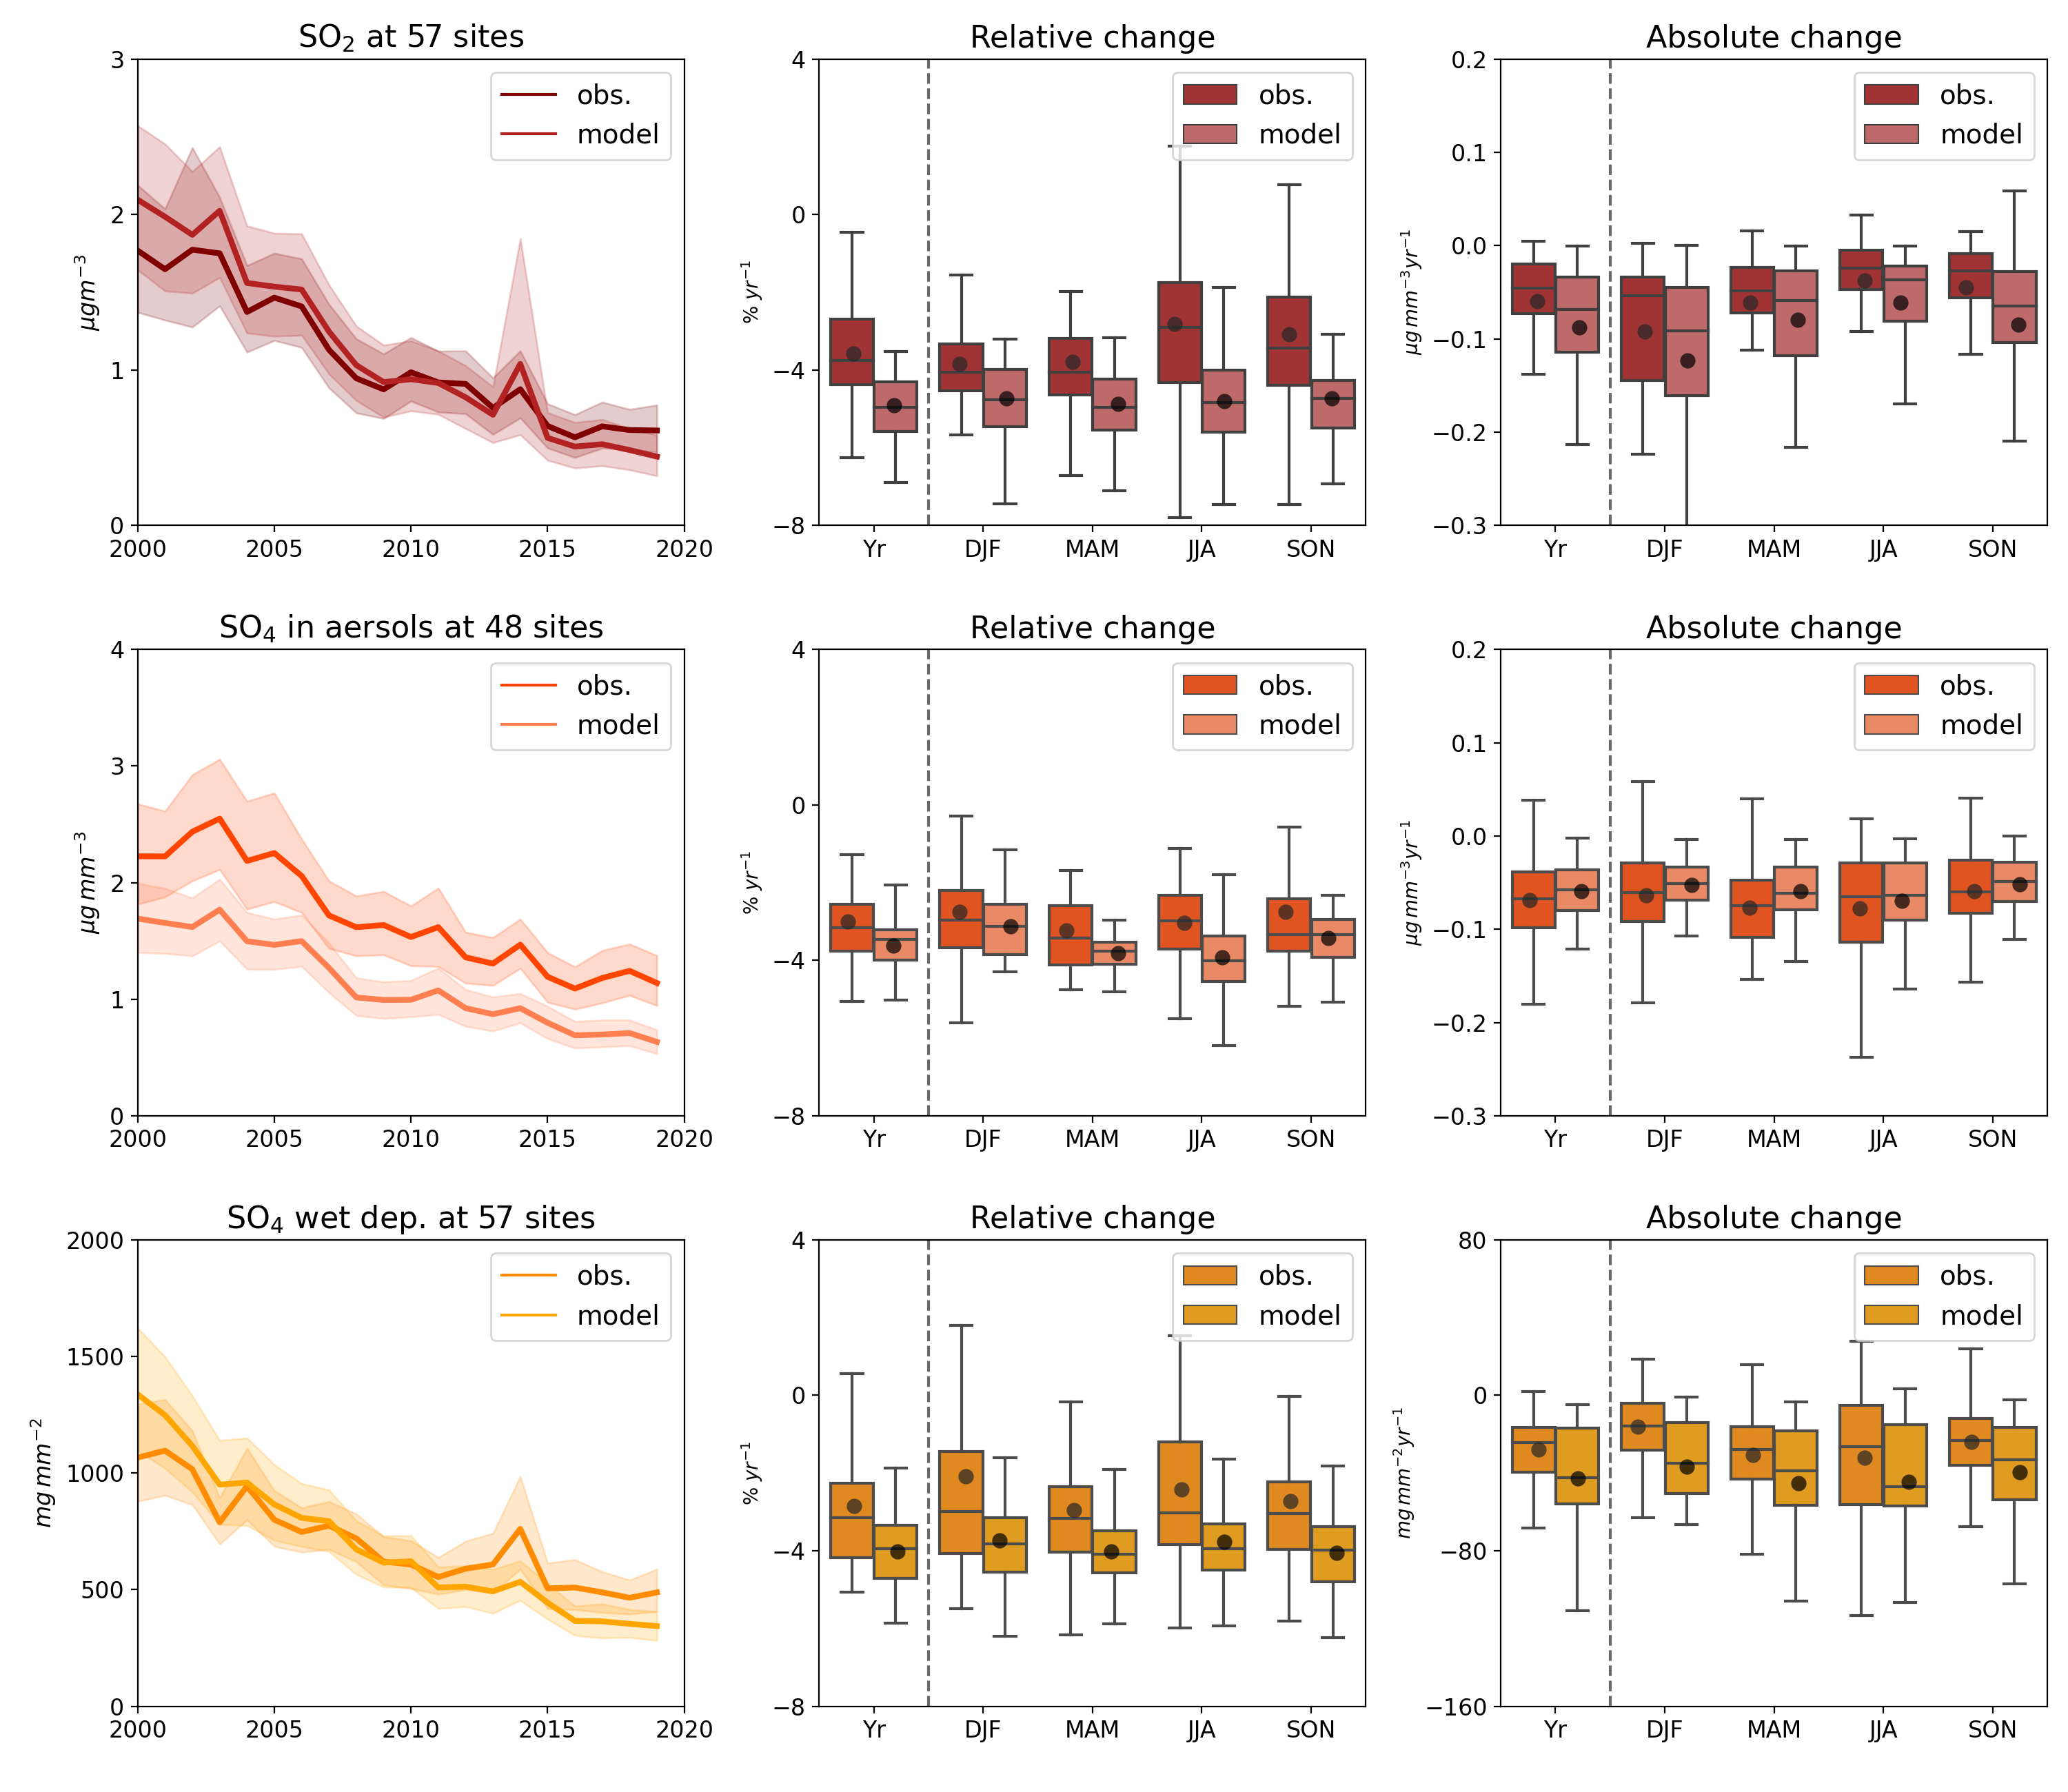
\includegraphics[width=0.74\paperwidth]{FIGS_TRENDS/sulfur_trends.png}
	\caption{\label{fig:SOx_trends}Trends in sulfur components from 2010-2019 for EMEP observations and model. The solid line in the trend plots indicate the average annual mean concentrations for all the sites and the shaded area the 95 \% confidence interval. The box plot represent the 50,25,75 percentiles and the whiskers lie within the 1.5 inter-quartile ranges for the trends of all the sites, including those with not significant trends. In addition, the mean trends are indicated with black circles and the trend in SOx emission is indicated in the plot of \soii with secondary y-axes}
\end{figure}

\begin{figure} [h]
  \centering{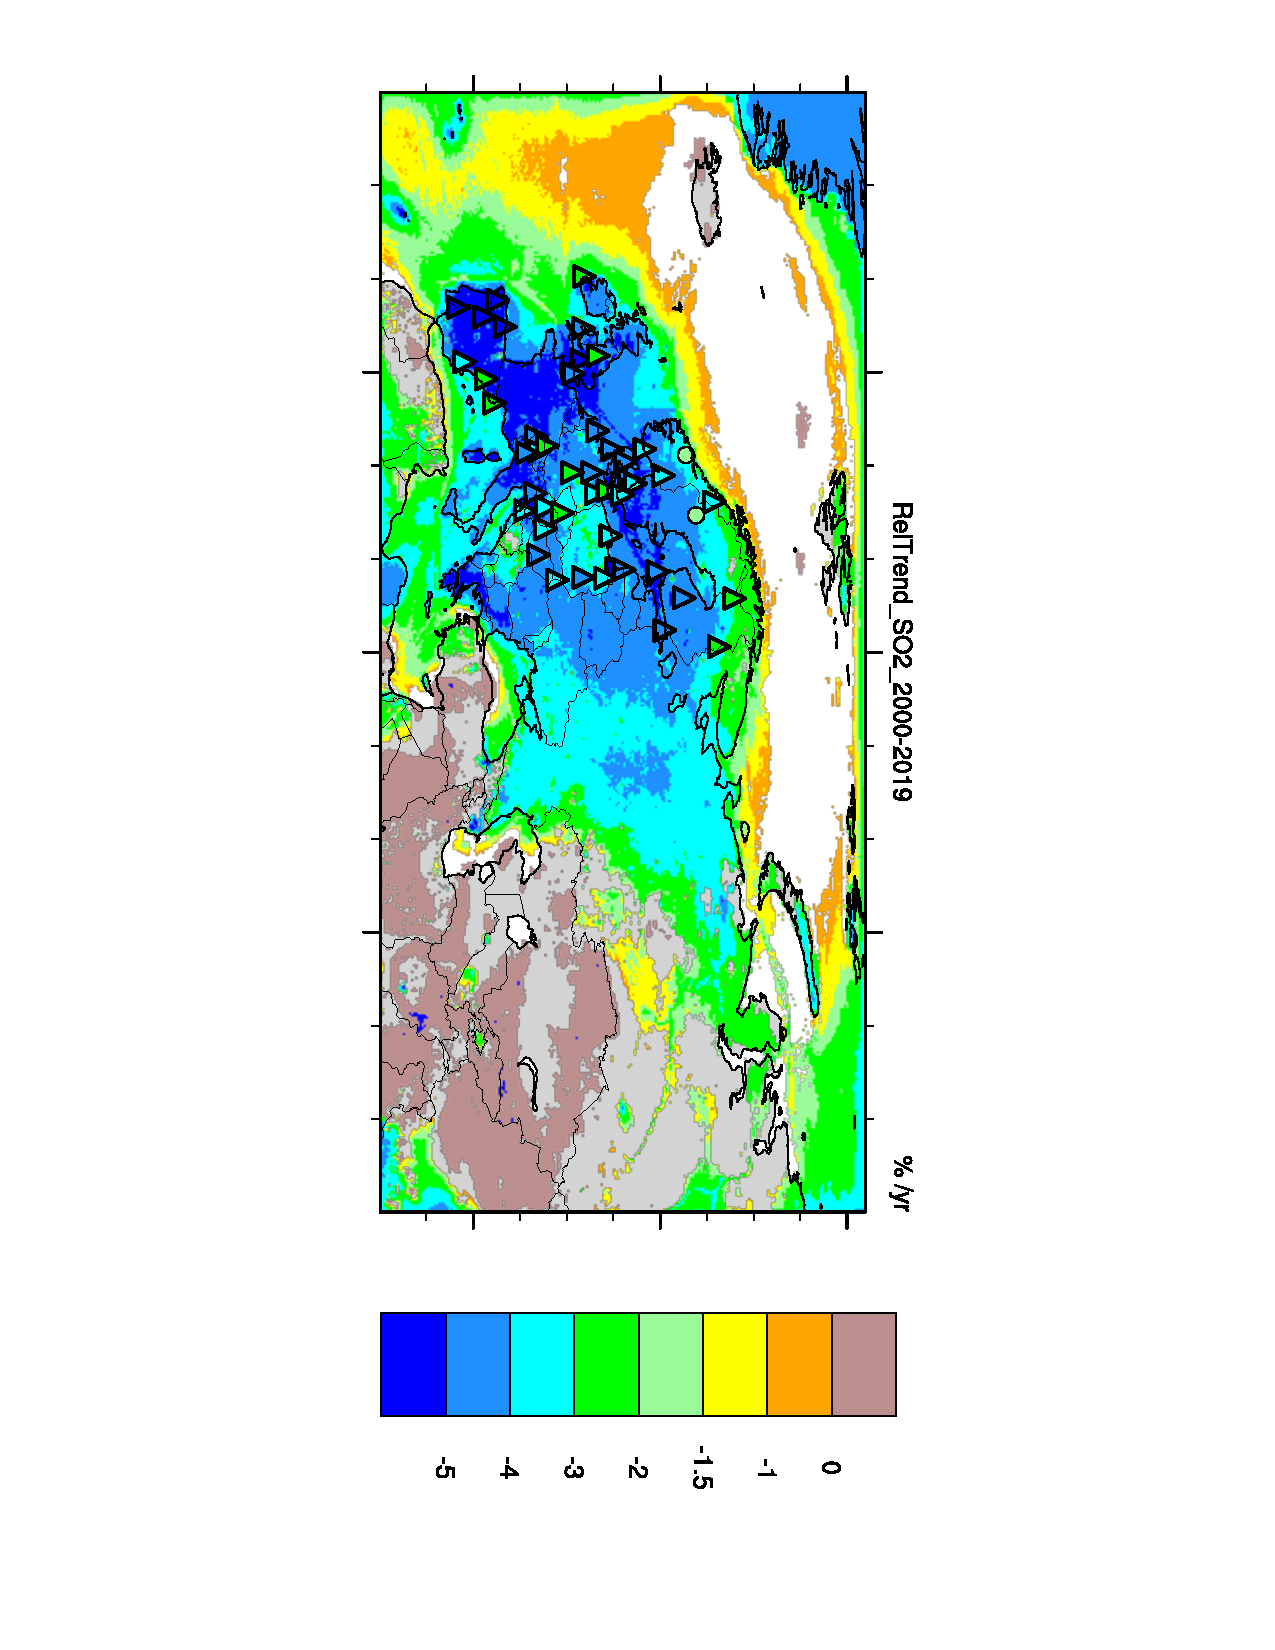
\includegraphics[clip=,angle=90,height=6.1cm,viewport=175 67 448 754]{FIGS_TRENDS/RelTrend_SO2_2000-2019_Perc.pdf}}\\
%  \vspace{0.5cm}
  \centering{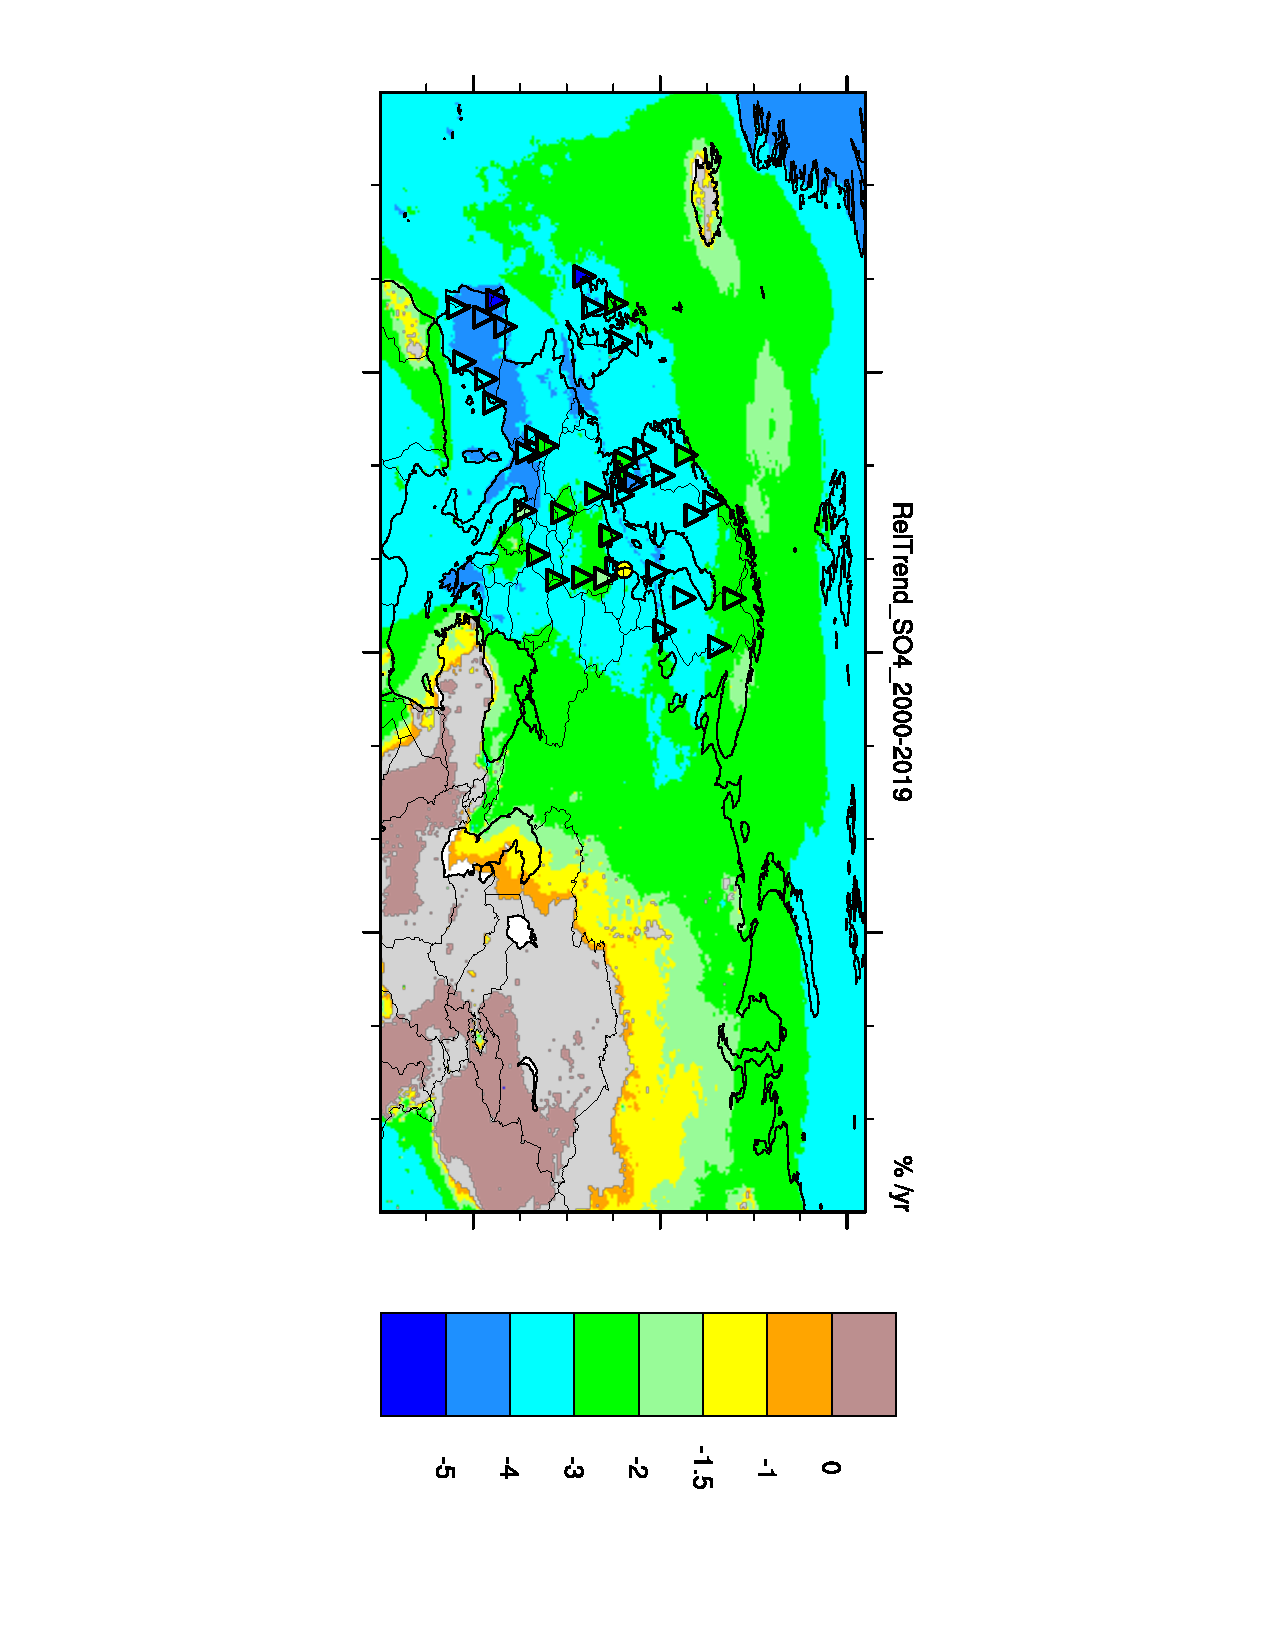
\includegraphics[clip=,angle=90,height=6.1cm,viewport=175 67 448 754]{FIGS_TRENDS/RelTrend_SO4_2000-2019_Perc.pdf}}
  %  \vspace{0.5cm}
  \centering{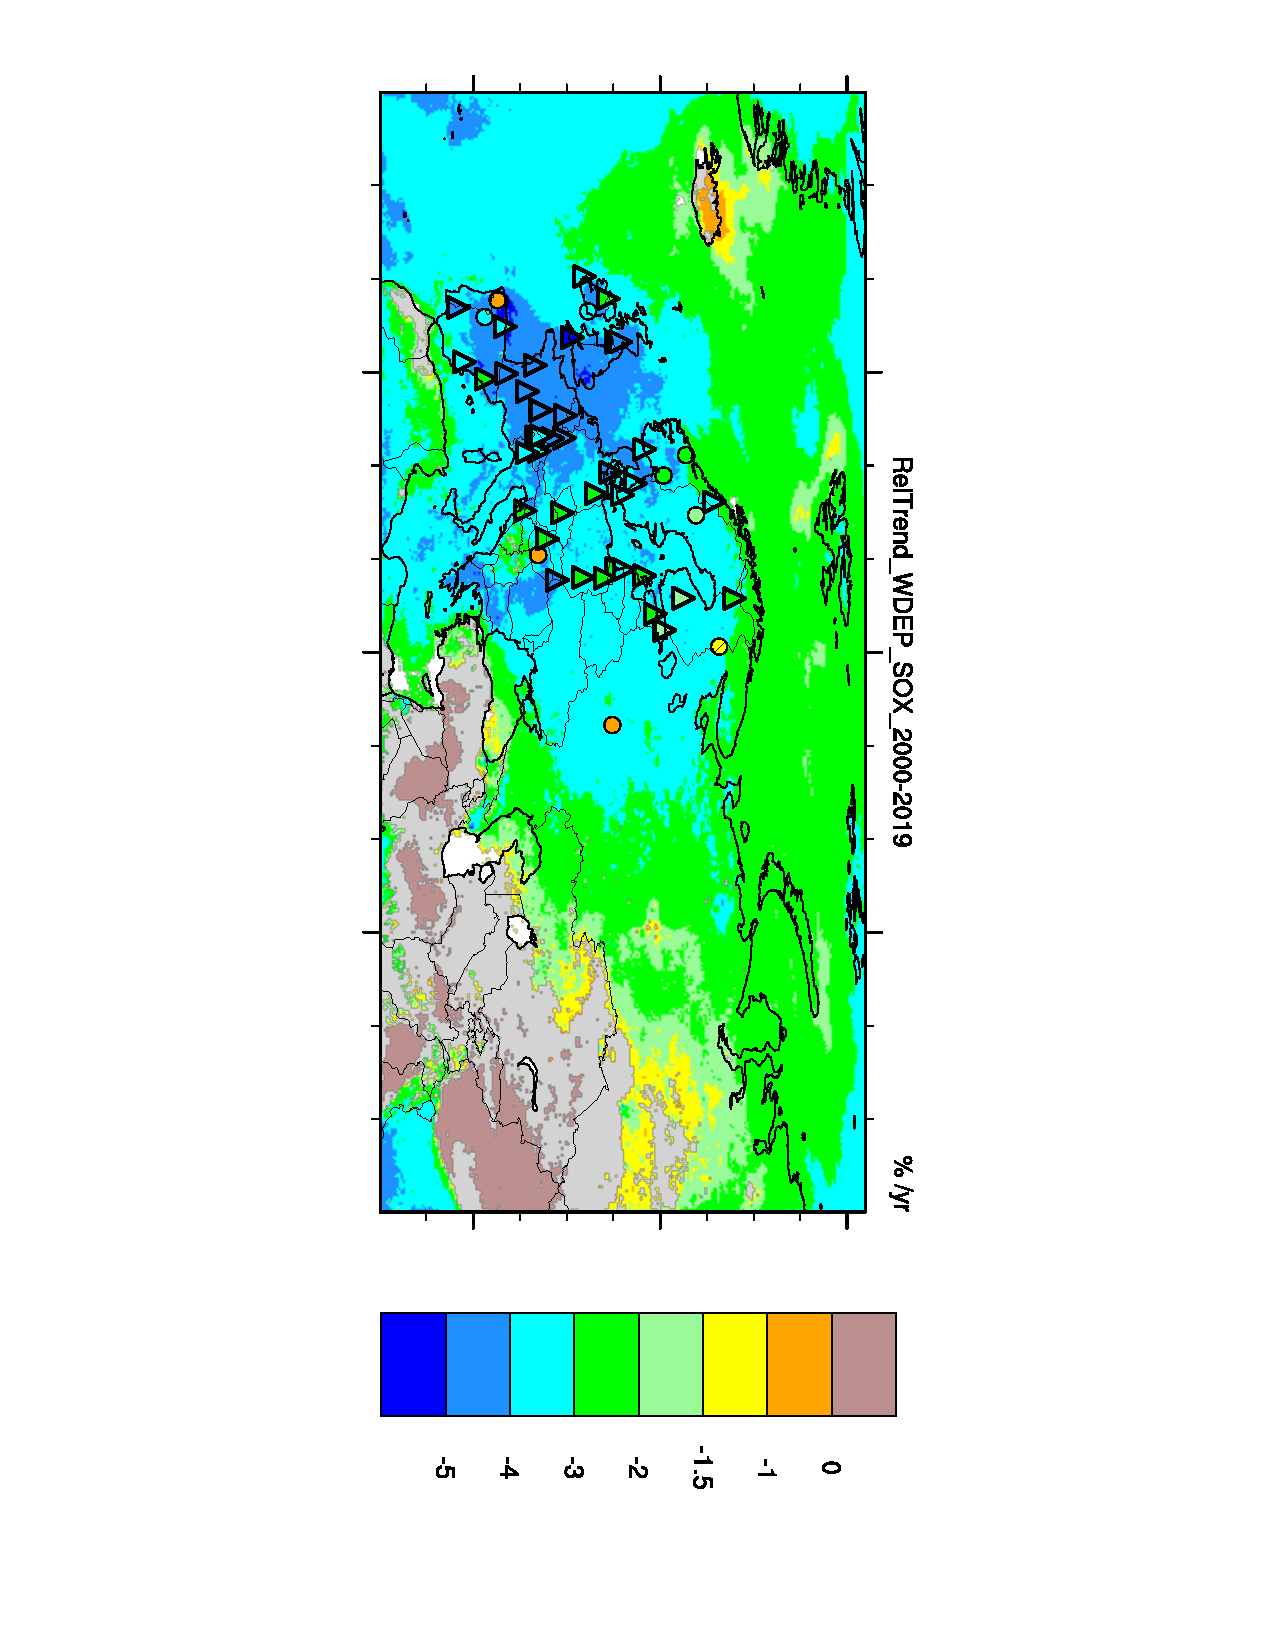
\includegraphics[clip=,angle=90,height=6.1cm,viewport=175 67 448 754]{FIGS_TRENDS/RelTrend_WDEP_SOX_2000-2019_Perc.pdf}}
\caption{Relative trends for \soii, \soiv in aerosols and wet deposition of \soiv in the period of 2000-2019: EMEP modelled -- coloured contours (grey/white means non-significant trends) and observed - coloured triangles (significant) and circles (non-significant).}
\label{fig:Strends_map}
\end{figure}



\begin{table}[h]
\caption{\label{tab:so2_stat} Absolute and relative change and corresponding 95\% confidence intervals in observed and modelled annual and seasonal aggregated \soii concentrations for the different time periods.The number of sites with a significant outcome is provided}
\begin{center}
\scalebox{0.65}{%
\begin{tabular}{ll|ccc|cccc|cccc}
\toprule
          &        & \multicolumn{3}{c}{Number of sites} & \multicolumn{4}{c}{Absolute change (\ug $yr^{-1})$} & \multicolumn{4}{c}{Relative change (\% $yr^{-1}$)} \\
Period & Seasons &           total & sign.(obs.) & sign.(mod.) &                    obs. &          conf.interval &  mod. &          conf.interval &                     obs. &         conf.interval &  mod. &        conf.interval \\
\midrule
2000-2019 & all &              48 &          46 &          48 &                  -0.068 &  (-0.085, -0.051) & -0.088 &  (-0.109, -0.067) &                    -3.88 &  (-4.23, -3.53) & -5.10 &  (-5.39, -4.81) \\
          & winter &              50 &          45 &          49 &                  -0.102 &  (-0.127, -0.076) & -0.124 &  (-0.153, -0.095) &                    -4.08 &   (-4.36, -3.8) & -4.94 &  (-5.22, -4.65) \\
          & spring &              48 &          45 &          48 &                  -0.070 &  (-0.086, -0.053) & -0.081 &  (-0.101, -0.061) &                    -4.15 &  (-4.45, -3.85) & -5.09 &  (-5.35, -4.84) \\
          & summer &              48 &          33 &          48 &                  -0.043 &  (-0.057, -0.029) & -0.060 &  (-0.078, -0.041) &                    -3.01 &  (-3.59, -2.43) & -4.94 &   (-5.3, -4.58) \\
          & autumn &              48 &          36 &          47 &                  -0.051 &  (-0.066, -0.035) & -0.086 &  (-0.107, -0.064) &                    -3.55 &  (-3.94, -3.15) & -5.02 &   (-5.3, -4.75) \\
2005-2019 & all &              57 &          41 &          54 &                  -0.055 &  (-0.068, -0.041) & -0.067 &   (-0.084, -0.05) &                    -4.27 &  (-4.72, -3.83) & -5.26 &   (-5.6, -4.93) \\
2010-2019 & all &              60 &          36 &          42 &                  -0.050 &  (-0.062, -0.037) & -0.056 &  (-0.072, -0.041) &                    -4.81 &  (-5.94, -3.69) & -6.39 &  (-7.15, -5.63) \\
2000-2010 & all &              66 &          30 &          58 &                  -0.079 &  (-0.103, -0.054) & -0.117 &  (-0.142, -0.091) &                    -3.52 &  (-4.31, -2.73) & -5.39 &  (-5.93, -4.84) \\
\bottomrule
\end{tabular}}
\end{center}
\end{table}

\begin{table}[h]
\caption{\label{tab:so4pm_stat} Absolute and relative change and corresponding 95\% confidence intervals in observed and modelled annual and seasonal aggregated \soiv concentrations for the different time periods.The number of sites with a significant outcome is provided}
\begin{center}
\scalebox{0.65}{%
\begin{tabular}{ll|ccc|cccc|cccc}
\toprule
          &        & \multicolumn{3}{c}{Number of sites} & \multicolumn{4}{c}{Absolute change (\ug $yr^{-1})$} & \multicolumn{4}{c}{Relative change (\% $yr^{-1}$)} \\
Period & Seasons &           total & sign.(obs.) & sign.(mod.) &                    obs. &          conf.interval &  mod. &          conf.interval &                     obs. &         conf.interval &  mod. &        conf.interval \\
\midrule
2000-2019 & all &              39 &          38 &          39 &                  -0.074 &  (-0.087, -0.062) & -0.065 &  (-0.076, -0.053) &                    -3.20 &  (-3.46, -2.93) & -3.81 &  (-4.04, -3.58) \\
          & winter &              40 &          29 &          34 &                  -0.064 &   (-0.08, -0.049) & -0.056 &  (-0.066, -0.046) &                    -2.75 &  (-3.22, -2.28) & -3.21 &  (-3.44, -2.97) \\
          & spring &              38 &          36 &          38 &                  -0.085 &  (-0.098, -0.072) & -0.065 &  (-0.075, -0.055) &                    -3.46 &  (-3.72, -3.19) & -4.03 &  (-4.21, -3.84) \\
          & summer &              38 &          36 &          38 &                  -0.082 &  (-0.102, -0.063) & -0.078 &  (-0.097, -0.059) &                    -3.15 &  (-3.46, -2.85) & -4.20 &   (-4.5, -3.91) \\
          & autumn &              37 &          34 &          37 &                  -0.062 &   (-0.073, -0.05) & -0.057 &  (-0.067, -0.046) &                    -3.08 &   (-3.4, -2.76) & -3.59 &  (-3.81, -3.38) \\
2005-2019 & all &              43 &          35 &          42 &                  -0.067 &  (-0.079, -0.055) & -0.054 &  (-0.063, -0.046) &                    -3.48 &  (-3.88, -3.09) & -4.01 &  (-4.25, -3.77) \\
2010-2019 & all &              46 &          20 &          32 &                  -0.053 &  (-0.068, -0.038) & -0.044 &  (-0.055, -0.034) &                    -3.43 &  (-4.11, -2.75) & -4.26 &  (-4.91, -3.62) \\
2000-2010 & all &              54 &          15 &          43 &                  -0.068 &  (-0.085, -0.051) & -0.094 &  (-0.109, -0.079) &                    -2.51 &  (-2.95, -2.07) & -4.19 &  (-4.52, -3.86) \\
\bottomrule
\end{tabular}}
\end{center}
\end{table}

\begin{table}[h]
\caption{\label{tab:so4dep_stat} Absolute and relative change and corresponding 95\%  confidence intervals in observed and modelled annual and seasonal aggregated wet deposition of sulfate for the different time periods.The number of sites with a significant outcome is provided}
\begin{center}
\scalebox{0.65}{%
\begin{tabular}{ll|ccc|cccc|cccc}
\toprule
          &        & \multicolumn{3}{c}{Number of sites} & \multicolumn{4}{c}{Absolute change (\ug $m^{2} yr^{-1}$)} & \multicolumn{4}{c}{Relative change (\% $yr^{-1}$)} \\
Period & Seasons &           total & sign.(obs.) & sign.(mod.) &                    obs. &          conf.interval &  mod. &          conf.interval &                     obs. &         conf.interval &  mod. &        conf.interval \\
\midrule
2000-2019 & all &              49 &          40 &          49 &                   -29.5 &  (-34.8, -24.2) & -48.1 &   (-56.9, -39.4) &                    -3.14 &  (-3.46, -2.82) & -4.27 &   (-4.5, -4.04) \\
          & winter &              47 &          25 &          44 &                   -19.5 &  (-24.5, -14.5) & -41.4 &   (-49.5, -33.3) &                    -2.87 &   (-3.34, -2.4) & -3.97 &  (-4.21, -3.73) \\
          & spring &              45 &          30 &          45 &                   -32.7 &  (-39.1, -26.2) & -49.2 &   (-59.7, -38.6) &                    -3.23 &   (-3.6, -2.86) & -4.19 &  (-4.41, -3.98) \\
          & summer &              47 &          31 &          45 &                   -36.5 &  (-44.5, -28.5) & -52.6 &   (-63.0, -42.2) &                    -2.95 &  (-3.35, -2.54) & -4.20 &  (-4.46, -3.94) \\
          & autumn &              46 &          27 &          42 &                   -26.7 &  (-32.3, -21.1) & -45.0 &   (-54.6, -35.5) &                    -3.00 &  (-3.49, -2.51) & -4.25 &  (-4.52, -3.99) \\
2005-2019 & all &              53 &          30 &          50 &                   -22.9 &  (-27.9, -17.9) & -36.3 &   (-42.4, -30.2) &                    -2.87 &  (-3.51, -2.22) & -4.53 &  (-4.79, -4.27) \\
2010-2019 & all &              60 &          15 &          40 &                   -20.9 &  (-27.1, -14.6) & -34.0 &   (-40.6, -27.3) &                    -2.86 &  (-3.78, -1.93) & -5.08 &  (-5.56, -4.59) \\
2000-2010 & all &              54 &          28 &          44 &                   -46.9 &  (-56.6, -37.1) & -68.5 &   (-81.4, -55.7) &                    -4.44 &  (-5.15, -3.74) & -5.29 &   (-5.68, -4.9) \\
\bottomrule
\end{tabular}}
\end{center}
\end{table}


\section{\label{sec:Trends_oxidised_nitrogen }Trends in oxidised nitrogen}

During the last decades, the total emissions of NO$_x$ declined significantly in Europe, followed by declining nitrogen dioxide concentrations, total nitrate (nitric acid plus particulate nitrate) in air and oxidized nitrogen wet deposition at EMEP background sites. This is found both for the EMEP MSC-W model calculations and for observations. Similar results have been presented in \citet{Theobald2019} for wet deposition of oxidized nitrogen for the 1990-2010 period and in \citet{Banzhaf2015} for total nitrate for 1990-2009. \citet{torseth2012} also find decreasing trends in nitrogen dioxide, total nitrate and nitrate in precipitations 1990-2009 in EMEP observations. A more recent study, analyzing the period 2000-2017 \citep{Colette2021} and including Airbase and most EMEP observations, also find decreasing trends in nitrogen dioxide.

Figure~\ref{fig:NOx_trends} shows an overview of the annual and seasonal trends in oxidised nitrogen compounds from 2000 to 2019. Tables~\ref{tab:no2_stat} to \ref{tab:no3dep_stat} show absolute and relative changes in the different oxidized nitrogen compounds.

From 2000-2019, the reductions have been on average -1.2\% yr$^{-1}$ for nitrogen dioxide concentrations at EMEP background sites (total -24\%). As NO$_2$ has a short lifetime, the trend in NO$_2$ is expected to reflect the trend in (local) emissions of NOx. During the 2000-2019 period, NO$_x$ emissions within the western EMEP domain (EU27+UK+EFTA countries), where the dominant part of the long term EMEP observations are situated, decreased by -48\%. EMEP/MSC-W model calculations follows the reported emission reductions closely (average reductions of -2.2\% yr$^{-1}$, or in total -42\% ). 
The agreement between the trends calculated from observations and from the model (and emissions) agree well for the last period (2010-2019), with trends around -2.3\% yr$^{-1}$, whilst the trend in the first period is substantially lower in the observations than in the model calculations (and emissions). From Figure~\ref{fig:NOx_trends} it can be seen that the agreement between observations and model calculations is excellent until around 2008, but that in the year 2009 and onwards the model (and emissions) is shifted down relative to the observations. Similar results have been found in \citep{Colette2021}.




The trends in wet deposition of oxidized nitrogen reflects the long range transported oxidized nitrogen (e.g. NO$_x$ that has been converted to nitric acid and particulate nitrate and then washed out by rain) and is less sensitive to local changes. Also the trends for wet deposition of nitrate are lower in the observations than in the model calculations (and emissions of NO$_x$) for the 2000-2019 period. Whilst the average trend in observations is -1.4\% yr$^{-1}$ (total of -26\%), the model calculates the trend at the same sites to be -2.1 \% yr$^{-1}$ (total of -40\%), close to the trends in emissions from the western EMEP domain (-48\%). The difference between the trend in observations (and emissions?) are largest during the first period, similar to the results for NO$_2$. However, the model overestimates nitrate wet deposition somewhat up to around 2010, and are then shifted downward and in very good agreement with observations for the years after. Note that the number of sites with significant trends for the shorter periods are small, and thus the results encumbered with more uncertainty.

For particulate nitrate, nitric acid and their sum the results are more complex. The number of sites are few (especially for nitric acid, with only 6 sites), the coverage of Europe more scattered and the quality of the measurements is worse. 

The modelled trends for 2000 to 2019 are all around -2 to -2.3\% per year for particulate nitrate, nitric acid and their sum - aligned with the results of NO$_2$, wet deposition of oxidized nitrogen and the emissions. The observations show a somewhat smaller negative trend of around -1.6\% yr$^{-1}$ for the sum and around -2\% yr$^{-1}$ both for particulate nitrate and nitric acid. For the shorter periods, the number of sites with significant trends are very small, both in the model calculations and the observations, and thus the results more uncertain.
However, for all the three observations, the trend in the first period (2000-2010) is smaller than the trend in the second period, whilst the model show a rather similar trend for the sum, and larger trends in the first period for the separate components.

In Figure~\ref{fig:OXNtrends}, the trends for the individual sites are visualized on a map on top of the EMEP MSC-W model calculations. For NO$_2$ and wet deposition of oxidized nitrogen, the trends in the observations on the eastern part of the domain are smaller and to a larger extent non significant, whilst the trends in the EMEP MSC-W model calculations are in general larger and more often significant. The reasons for these discrepancies are not clear, but could be related to problems/inaccuracies in emission reporting and their trends, processes that are not (well enough) taken into account or in the observations themselves.

In summary we find that oxidized nitrogen in air and precipitation has been decreasing since 2000. However, the decrease in the observations (-24\% for NO2 and -26\% for wet deposition of oxidized nitrogen) are smaller than in model calculations (-42\% for NO2 and -40\% for wet deposition of oxidized nitrogen) and emissions (-48\% for EU27+UK+EFTA). 

\begin{figure}[h]
	\centering
	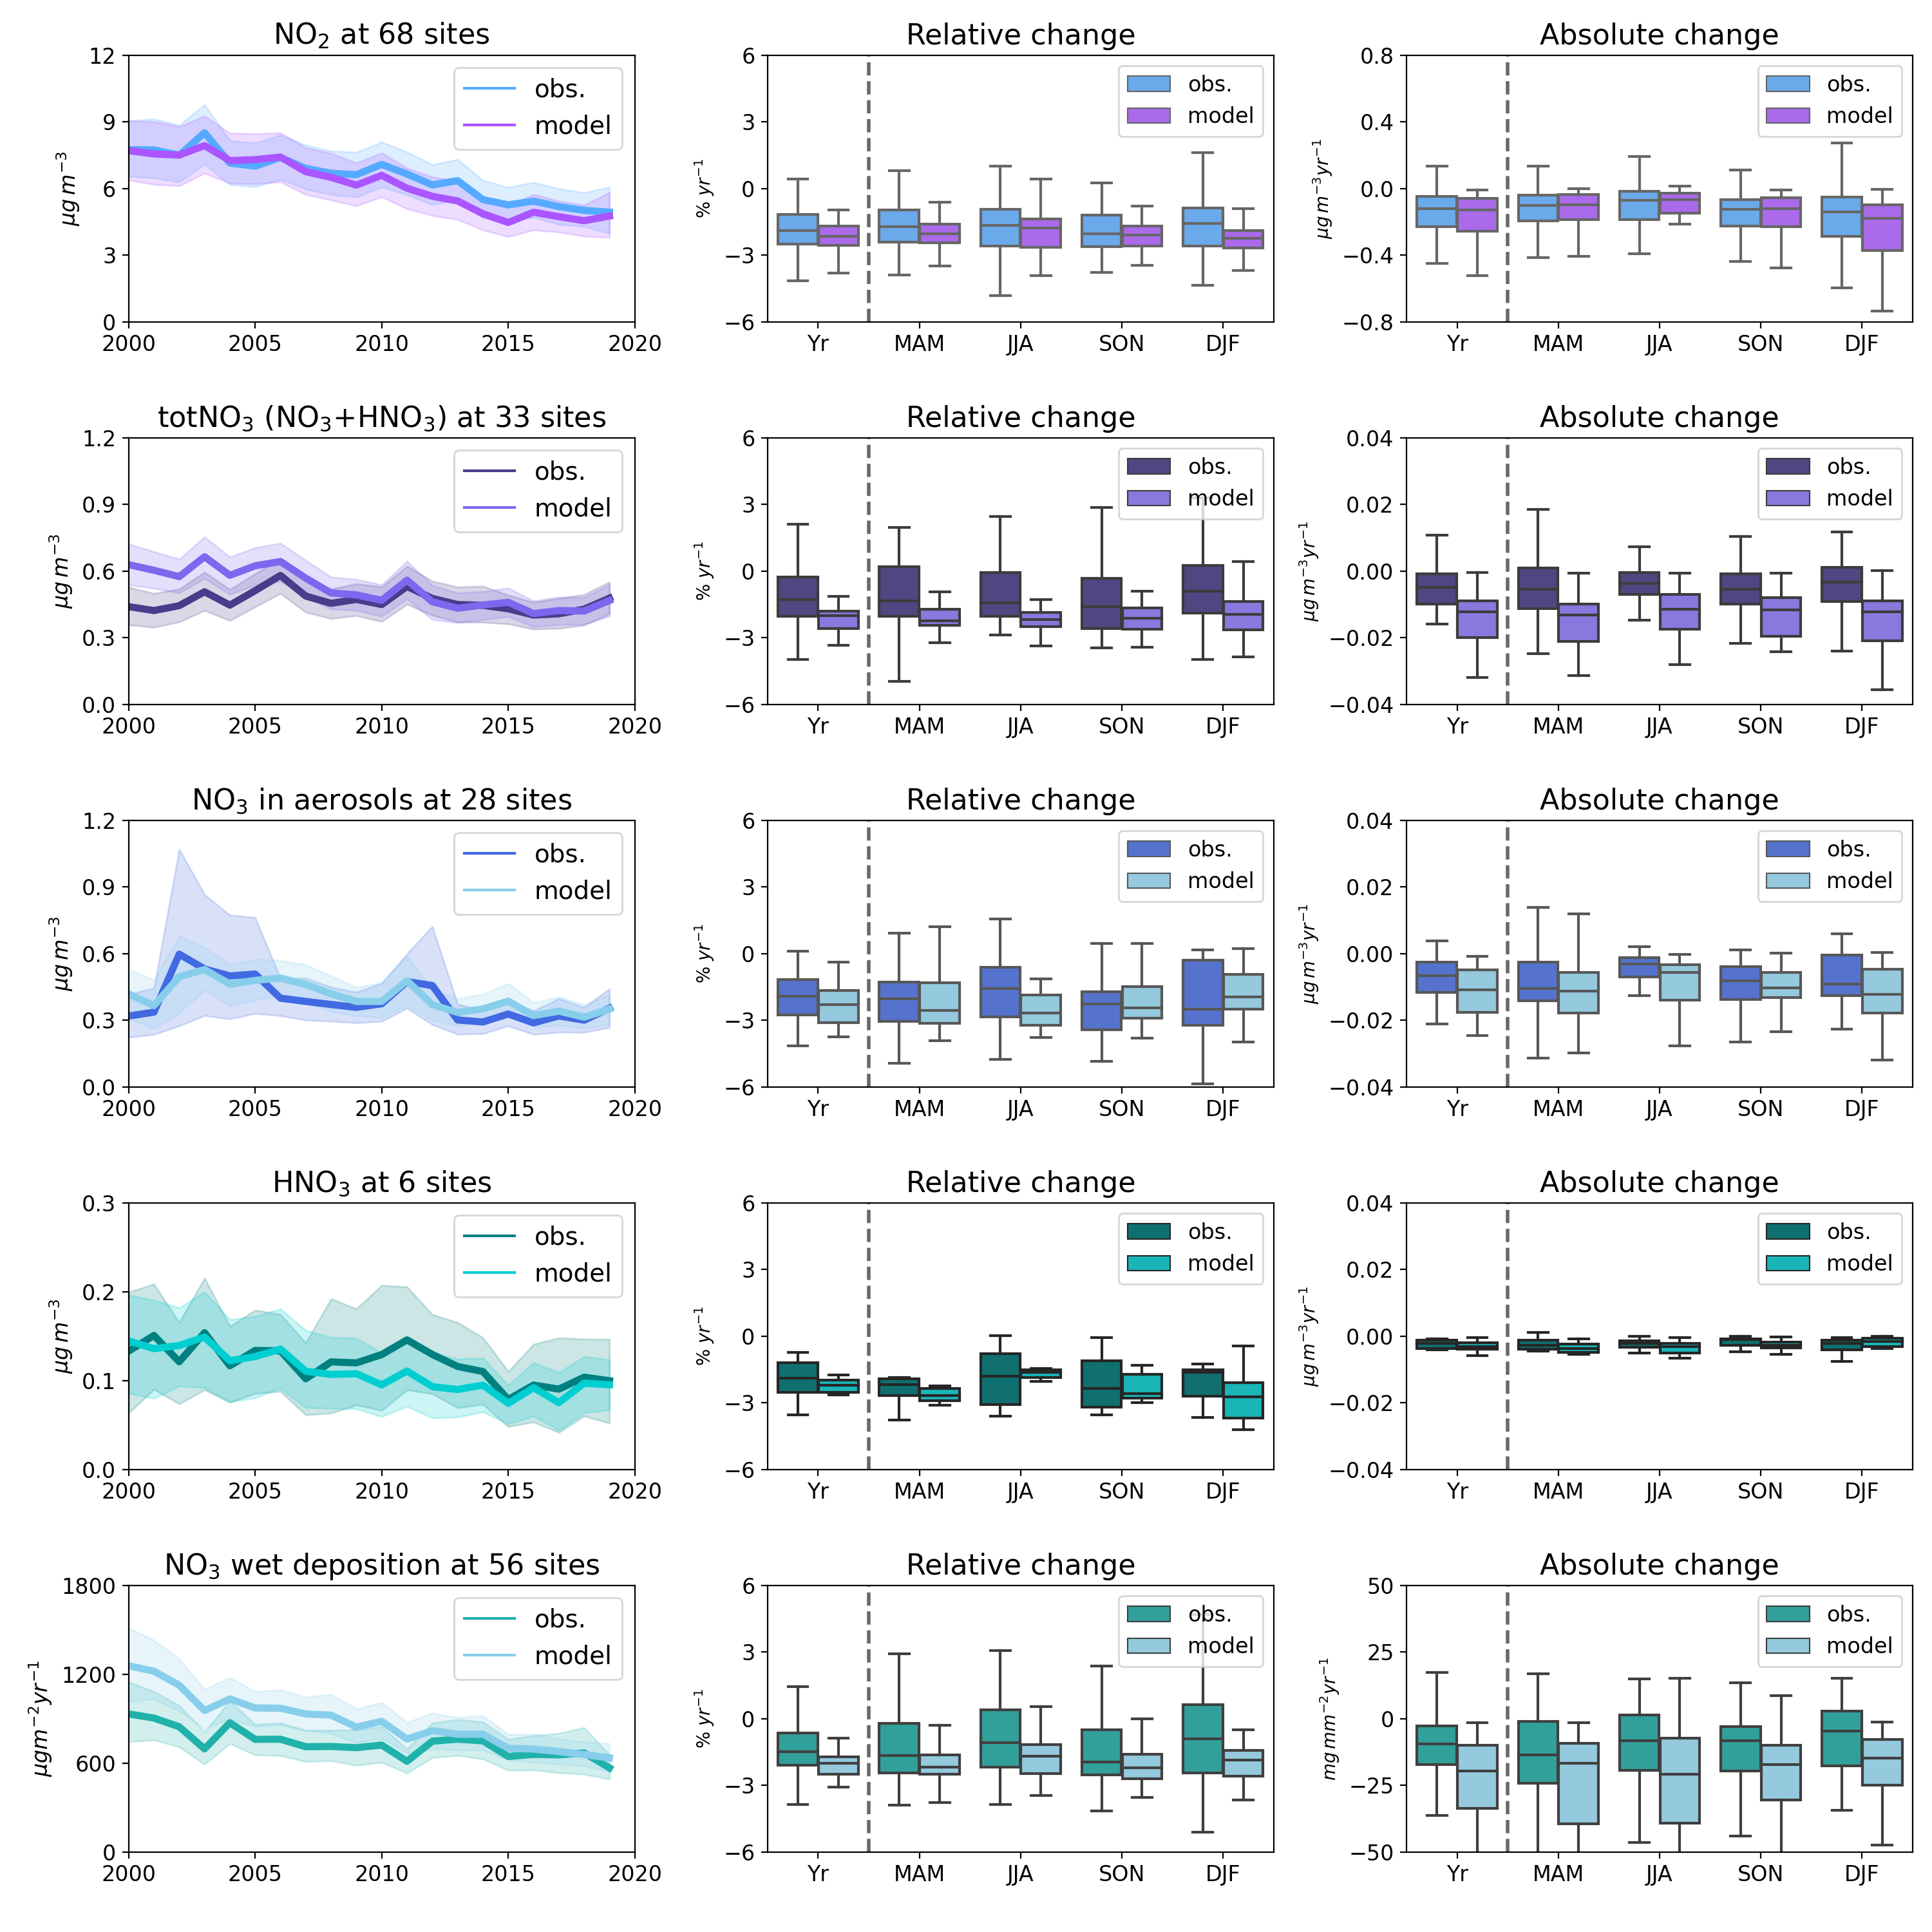
\includegraphics[width=0.74\paperwidth]{FIGS_TRENDS/Nox_trends.png}
	\caption{\label{fig:NOx_trends}Trends in oxidised nitrogen compounds from 2010-2019 for EMEP observations and model. The solid line in the trend plots indicate the average annual mean concentrations for all the sites and the shaded area the 95 \% confidence interval. The box plot represent the 50,25,75 percentiles and the whiskers lie within the 1.5 inter-quartile ranges for the trends of all the sites, including those with not significant trends. In addition, the mean trends are indicated with black circles and the trend in NOx emission is indicated in the plot of \noii with secondary y-axes}
\end{figure}

\begin{figure}[h]
  \centering{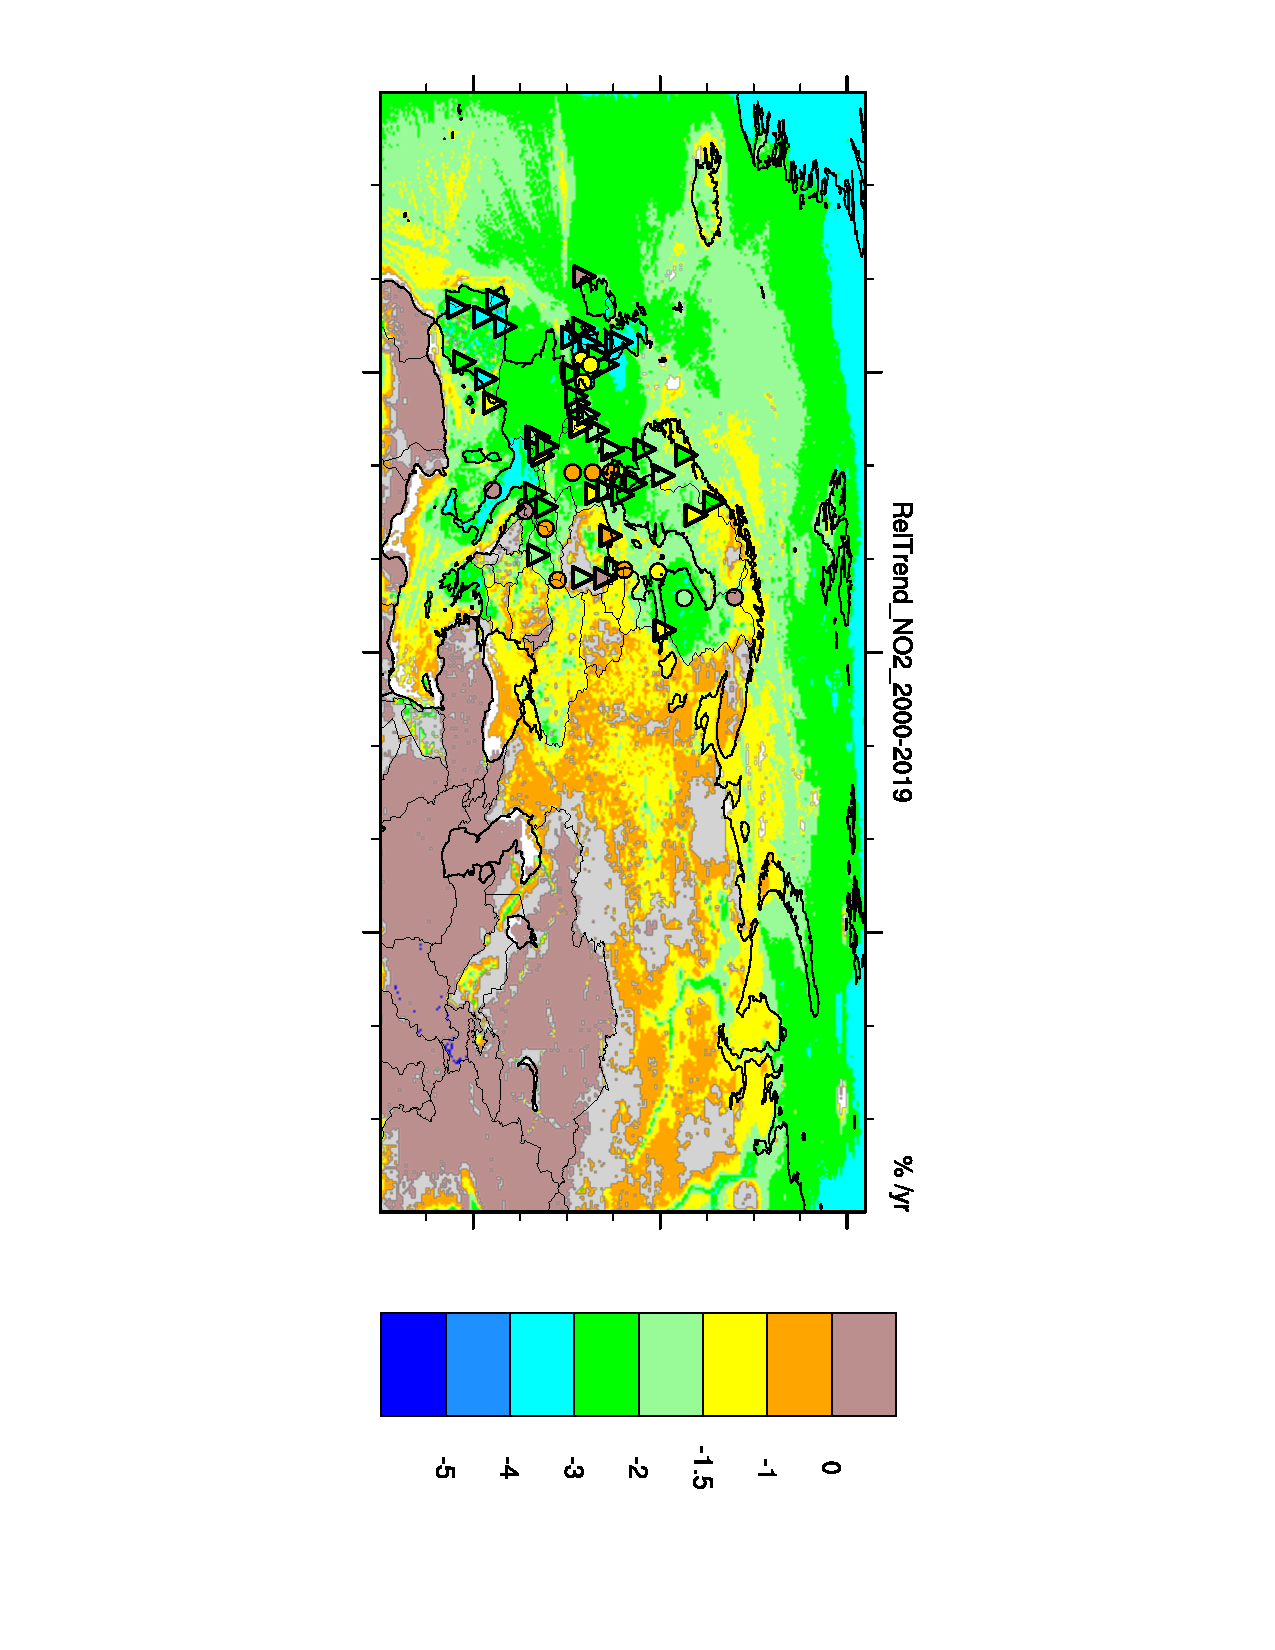
\includegraphics[clip=,angle=90,height=6.1cm,viewport=175 67 448 754]{FIGS_TRENDS/RelTrend_NO2_2000-2019_Perc.pdf}}
%  \vspace{0.5cm}
  \centering{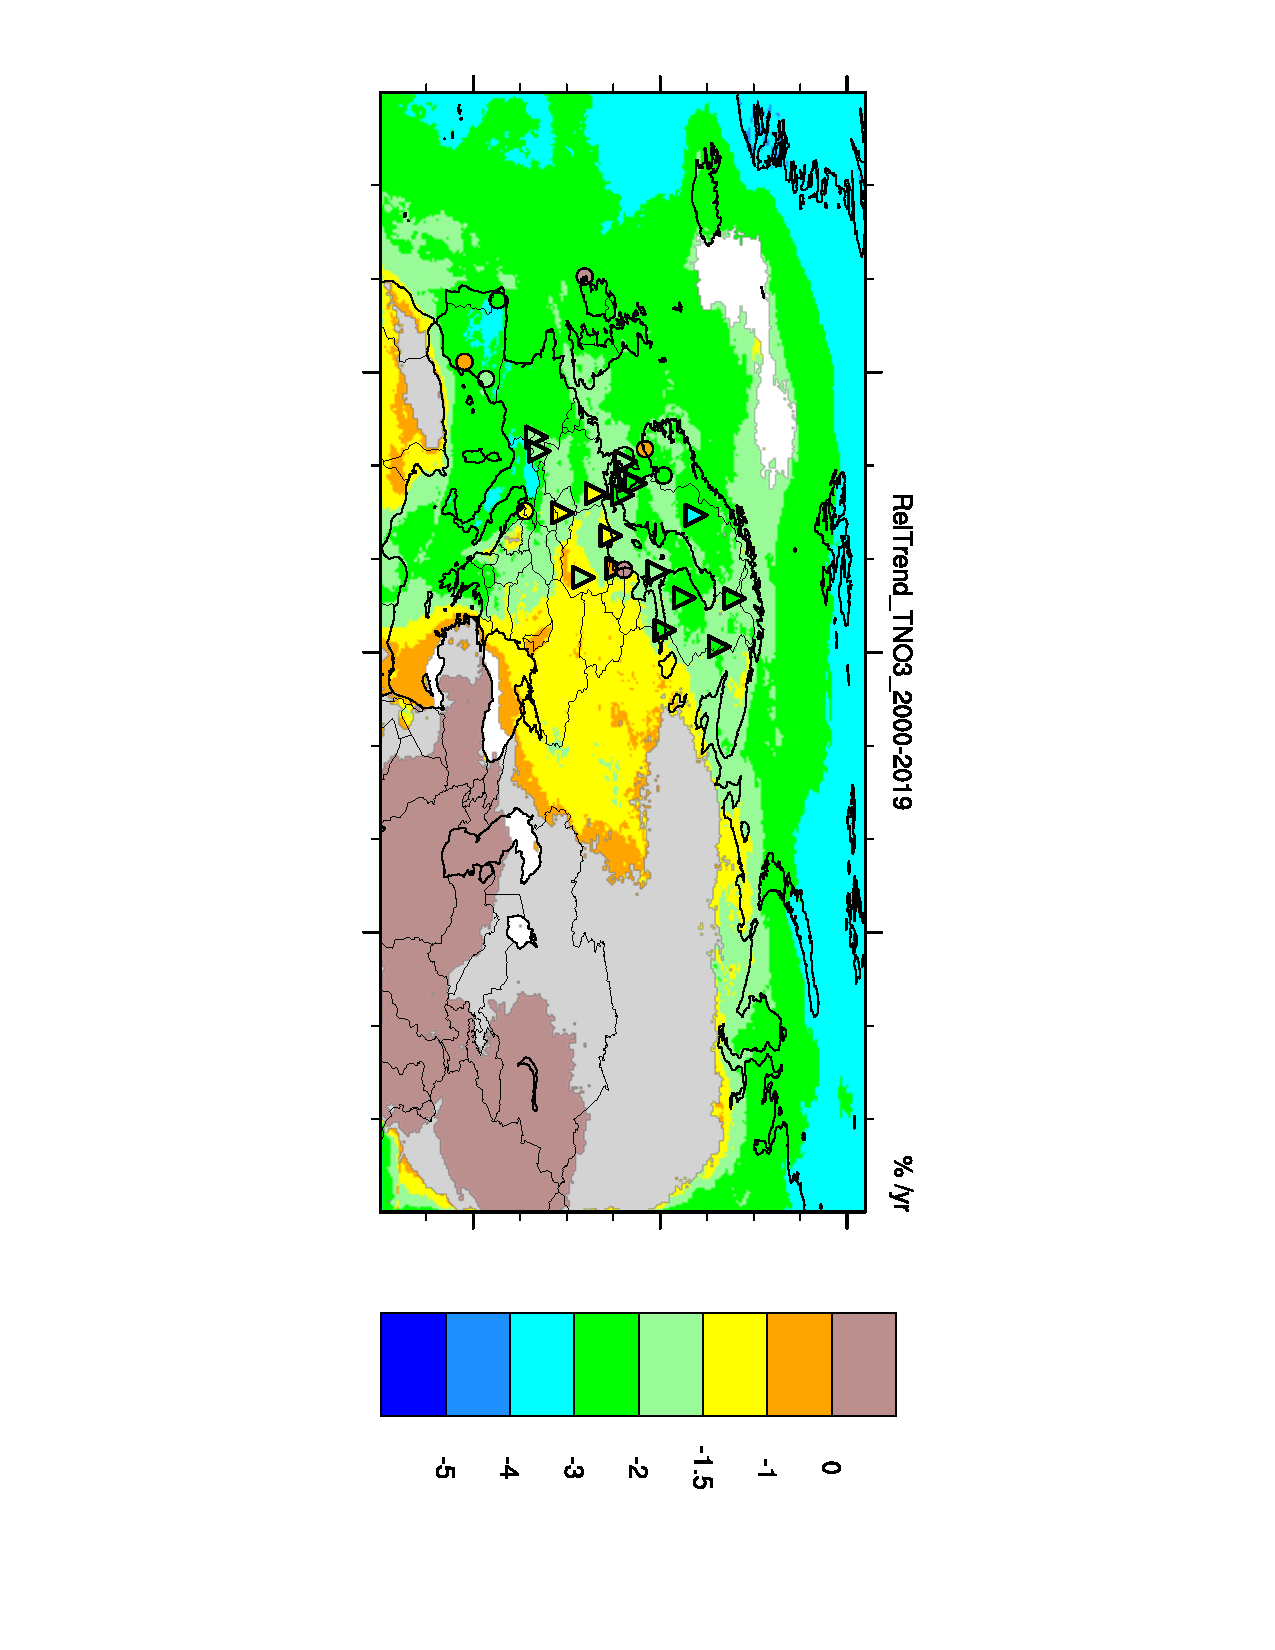
\includegraphics[clip=,angle=90,height=6.1cm,viewport=175 67 448 754]{FIGS_TRENDS/RelTrend_TNO3_2000-2019_Perc.pdf}}
\centering{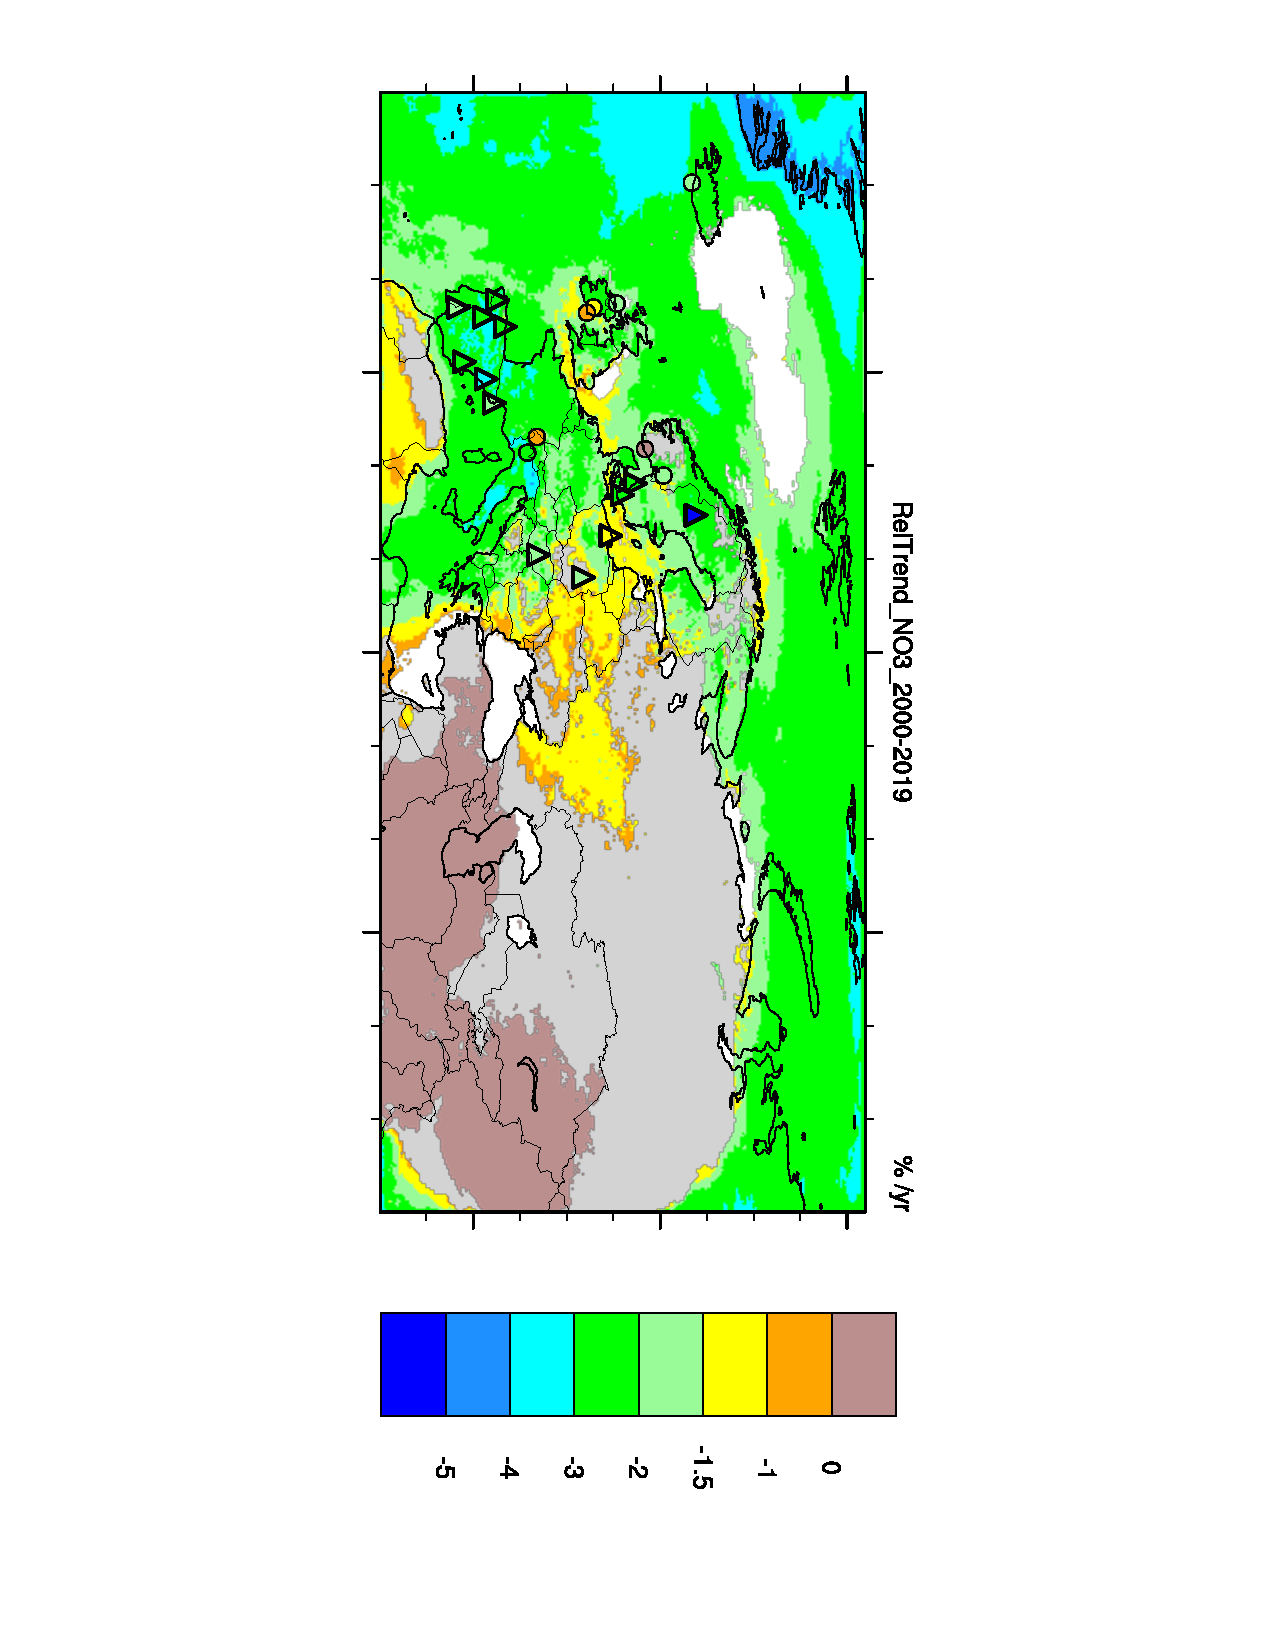
\includegraphics[clip=,angle=90,height=6.1cm,viewport=175 67 448 754]{FIGS_TRENDS/RelTrend_NO3_2000-2019_Perc.pdf}}
\centering{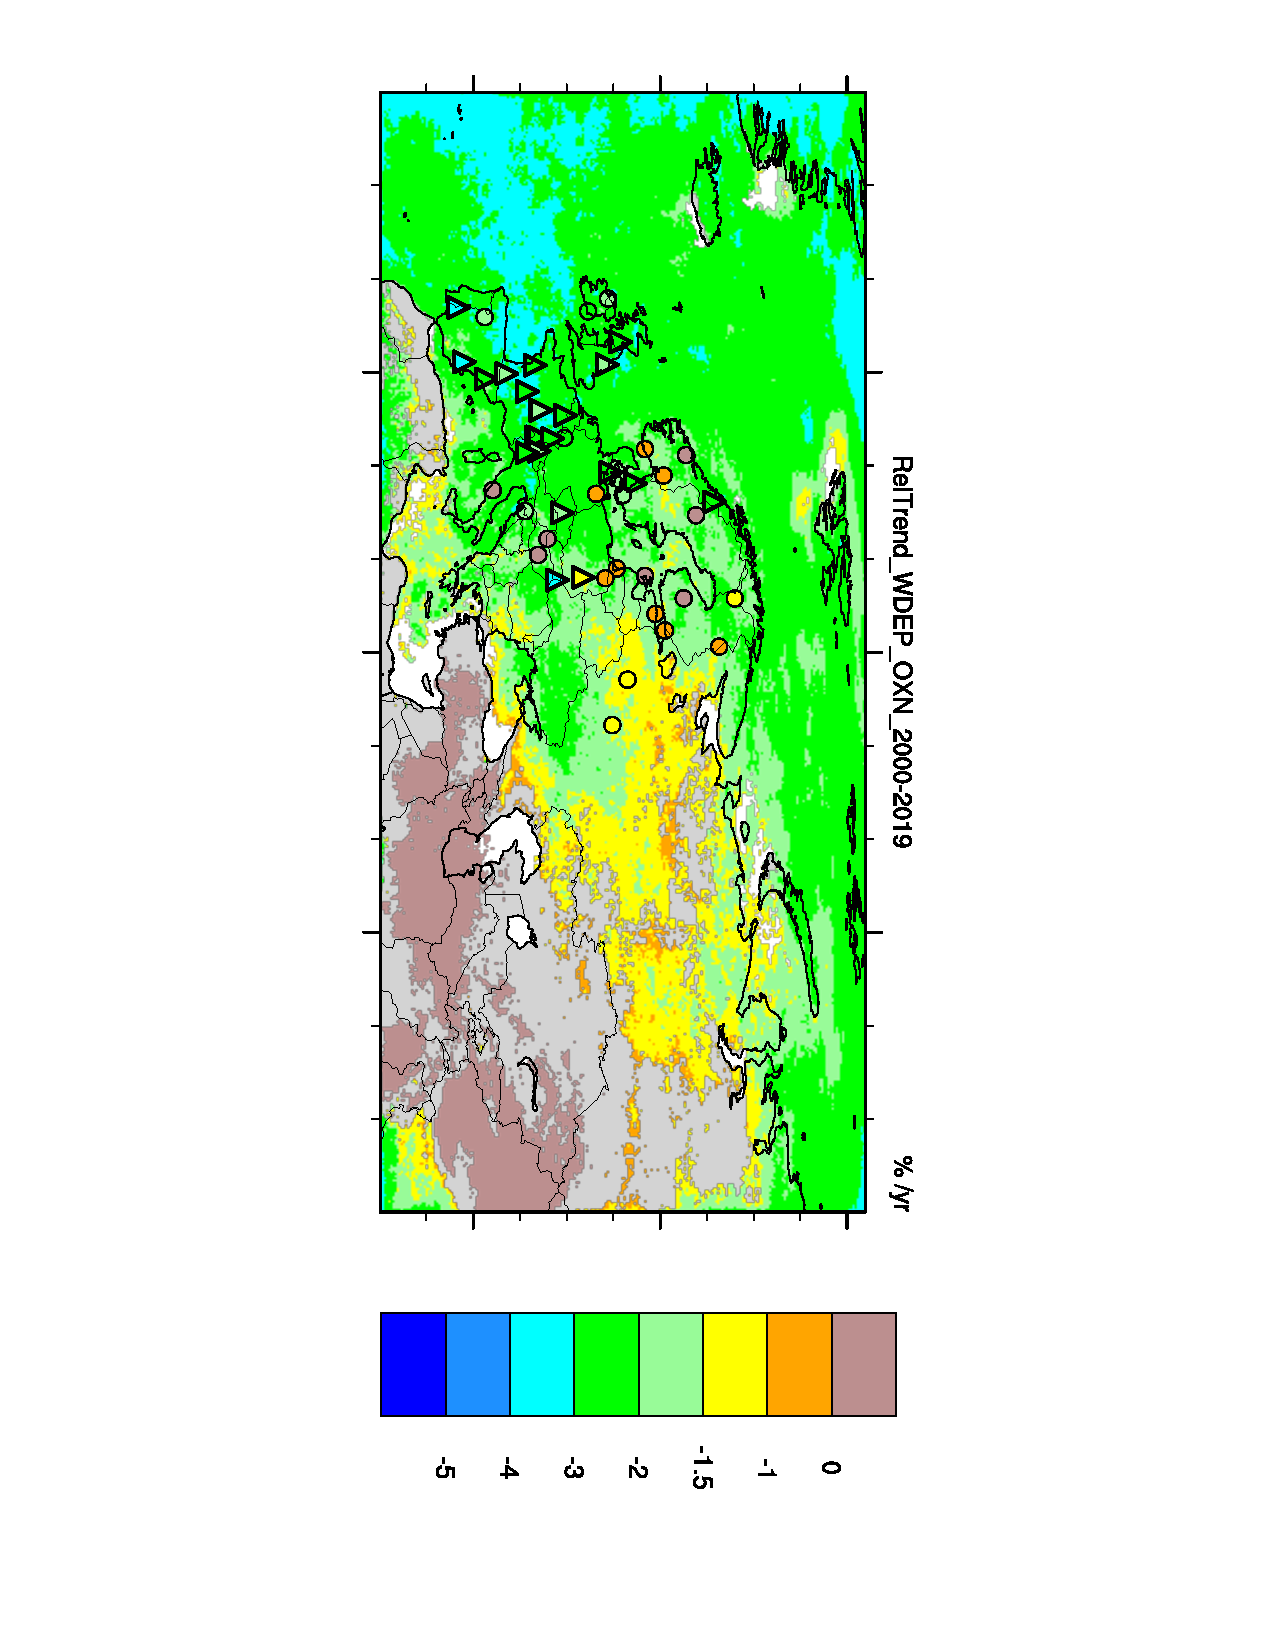
\includegraphics[clip=,angle=90,height=6.1cm,viewport=175 67 448 754]{FIGS_TRENDS/RelTrend_WDEP_OXN_2000-2019_Perc.pdf}}
\caption{Relative trends for NO$_2$, total nitrate, nitrate aerosol and wet deposition of oxidized nitrogen in the period of 2000-2019: EMEP modelled -- coloured contours (grey/white means non-significant trends) and
observed - coloured triangles (significant) and circles (non-significant).}
\label{fig:OXNtrends}
\end{figure}

\begin{table}[h]
\caption{\label{tab:no2_stat} Absolute and relative change and corresponding 95\% confidence intervals in observed and modelled annual and seasonal aggregated \noii concentrations for the different time periods. The number of sites with a significant outcome is provided}
\begin{center}
\scalebox{0.65}{%
\begin{tabular}{ll|ccc|cccc|cccc}
\toprule
          &        & \multicolumn{3}{c}{Number of sites} & \multicolumn{4}{c}{Average change (\ug $yr^{-1})$} & \multicolumn{4}{c}{Relative change (\% $yr^{-1}$)} \\
Period & Seasons &           total & sign.(obs.) & sign.(mod.) &                    obs. &          conf.interval &  mod. &          conf.interval &                     obs. &         conf.interval &  mod. &        conf.interval \\
\midrule
2000-2019 & all &              60 &          45 &          59 &                  -0.131 &    (-0.162, -0.1) & -0.191 &  (-0.235, -0.147) &                    -1.18 &  (-2.21, -0.15) & -2.25 &  (-2.42, -2.07) \\
          & winter &              61 &          30 &          58 &                  -0.151 &  (-0.192, -0.111) & -0.256 &  (-0.303, -0.209) &                    -1.13 &  (-2.03, -0.22) & -2.36 &  (-2.54, -2.19) \\
          & spring &              59 &          37 &          55 &                  -0.119 &   (-0.15, -0.088) & -0.158 &  (-0.201, -0.116) &                    -0.88 &   (-2.09, 0.32) & -2.07 &  (-2.26, -1.88) \\
          & summer &              59 &          39 &          55 &                  -0.092 &  (-0.118, -0.067) & -0.132 &   (-0.174, -0.09) &                    -1.18 &  (-2.07, -0.29) & -1.88 &  (-2.12, -1.64) \\
          & autumn &              59 &          41 &          58 &                  -0.149 &  (-0.186, -0.112) & -0.189 &  (-0.236, -0.141) &                    -1.13 &   (-2.41, 0.15) & -2.19 &  (-2.37, -2.01) \\
2005-2019 & all &              64 &          49 &          63 &                  -0.160 &  (-0.195, -0.125) & -0.194 &  (-0.237, -0.152) &                    -1.86 &  (-2.56, -1.16) & -2.58 &   (-2.8, -2.36) \\
2010-2019 & all &              66 &          36 &          52 &                  -0.184 &  (-0.226, -0.142) & -0.174 &  (-0.212, -0.135) &                    -2.65 &  (-3.39, -1.92) & -2.62 &  (-2.89, -2.35) \\
2000-2010 & all &              64 &          11 &          42 &                  -0.093 &  (-0.141, -0.044) & -0.181 &   (-0.231, -0.13) &                    -1.00 &  (-1.74, -0.27) & -1.98 &  (-2.36, -1.61) \\
\bottomrule
\end{tabular}}
\end{center}
\end{table}



\begin{table}[h]
\caption{\label{tab:tno3_stat} Absolute and relative change and corresponding 95\% confidence intervals in observed and modelled annual and seasonal aggregated concentrations of total nitrate ({\ensuremath{\mbox{HNO}_{\rm 3}}} + \noiii) in air and aerosols. The number of sites with a significant outcome is provided}
\begin{center}
\scalebox{0.65}{%
\begin{tabular}{ll|ccc|cccc|cccc}
\toprule
          &        & \multicolumn{3}{c}{Number of sites} & \multicolumn{4}{c}{Absolute change (\ug $yr^{-1})$} & \multicolumn{4}{c}{Relative change (\% $yr^{-1}$)} \\
Period & Seasons &           total & sign.(obs.) & sign.(mod.) &                    obs. &          conf.interval &  mod. &          conf.interval &                     obs. &         conf.interval &  mod. &        conf.interval \\
\midrule
2000-2019 & all &              25 &          17 &          25 &                  -0.008 &  (-0.011, -0.005) & -0.013 &   (-0.016, -0.01) &                    -1.60 &    (-2.0, -1.2) & -2.13 &  (-2.33, -1.94) \\
          & winter &              27 &           7 &          16 &                  -0.009 &  (-0.014, -0.003) & -0.014 &   (-0.018, -0.01) &                    -1.21 &  (-1.75, -0.66) & -1.93 &   (-2.26, -1.6) \\		  
          & spring &              25 &          13 &          21 &                  -0.010 &  (-0.013, -0.007) & -0.015 &  (-0.018, -0.011) &                    -1.69 &  (-2.08, -1.29) & -2.24 &  (-2.46, -2.02) \\
          & summer &              25 &          17 &          23 &                  -0.005 &  (-0.007, -0.003) & -0.012 &  (-0.015, -0.009) &                    -1.43 &   (-1.86, -1.0) & -2.27 &   (-2.43, -2.1) \\
          & autumn &              24 &          16 &          16 &                  -0.009 &  (-0.013, -0.006) & -0.014 &   (-0.019, -0.01) &                    -1.89 &  (-2.43, -1.35) & -2.20 &  (-2.48, -1.93) \\
2005-2019 & all &              31 &          18 &          26 &                  -0.011 &  (-0.014, -0.008) & -0.014 &  (-0.017, -0.011) &                    -2.29 &  (-2.74, -1.84) & -2.51 &   (-2.8, -2.22) \\
2010-2019 & all &              29 &          16 &           9 &                  -0.015 &   (-0.019, -0.01) & -0.010 &  (-0.014, -0.007) &                    -3.38 &   (-4.26, -2.5) & -2.16 &  (-2.58, -1.75) \\
2000-2010 & all &              33 &           7 &          11 &                  -0.006 &  (-0.011, -0.001) & -0.017 &  (-0.022, -0.012) &                    -0.54 &   (-1.55, 0.47) & -2.12 &  (-2.66, -1.57) \\
\bottomrule
\end{tabular}}
\end{center}
\end{table}

\begin{table}[h]
\caption{\label{tab:no3pm_stat}  Absolute and relative change and corresponding 95\% confidence intervals in observed and modelled annual and seasonal aggregated concentrations of  \noiii concentrations in aerosols. The number of sites with a significant outcome is provided}
\begin{center}
\scalebox{0.65}{%
\begin{tabular}{ll|ccc|cccc|cccc}
\toprule
          &        & \multicolumn{3}{c}{Number of sites} & \multicolumn{4}{c}{Absolute change (\ug $yr^{-1})$} & \multicolumn{4}{c}{Relative change (\% $yr^{-1}$)} \\
Period & Seasons &           total & sign.(obs.) & sign.(mod.) &                    obs. &          conf.interval &  mod. &          conf.interval &                     obs. &         conf.interval &  mod. &        conf.interval \\
\midrule
2000-2019 & all &              21 &          13 &          15 &                  -0.009 &  (-0.012, -0.006) & -0.014 &  (-0.018, -0.009) &                    -2.01 &  (-2.49, -1.53) & -2.53 &   (-2.86, -2.2) \\
          & winter &              20 &           8 &           5 &                  -0.012 &  (-0.018, -0.005) & -0.012 &  (-0.016, -0.008) &                    -1.85 &  (-2.77, -0.93) & -2.01 &  (-2.55, -1.47) \\
          & spring &              20 &          12 &          15 &                  -0.011 &  (-0.017, -0.005) & -0.012 &  (-0.018, -0.007) &                    -1.89 &  (-2.69, -1.09) & -2.21 &  (-2.97, -1.45) \\
          & summer &              20 &           8 &          13 &                  -0.004 &  (-0.006, -0.002) & -0.010 &  (-0.014, -0.006) &                    -1.55 &  (-2.17, -0.94) & -2.70 &  (-2.98, -2.43) \\
          & autumn &              20 &          11 &           9 &                  -0.010 &  (-0.013, -0.007) & -0.014 &  (-0.021, -0.007) &                    -2.41 &   (-2.8, -2.01) & -2.42 &  (-2.83, -2.01) \\
2005-2019 & all &              26 &          11 &          16 &                  -0.011 &  (-0.015, -0.006) & -0.014 &  (-0.018, -0.009) &                    -2.32 &  (-2.84, -1.81) & -2.77 &  (-3.21, -2.33) \\
2010-2019 & all &              32 &           3 &           6 &                  -0.010 &  (-0.015, -0.004) & -0.009 &  (-0.013, -0.005) &                    -1.98 &  (-2.85, -1.11) & -1.46 &  (-2.23, -0.68) \\
2000-2010 & all &              20 &           3 &           9 &                  -0.006 &   (-0.013, 0.001) & -0.020 &  (-0.028, -0.012) &                    -1.54 &   (-2.8, -0.27) & -3.01 &  (-3.99, -2.03) \\
\bottomrule
\end{tabular}}
\end{center}
\end{table}

\begin{table}[h]
\caption{\label{tab:hno3_stat} Absolute and relative change and corresponding 95\% confidence intervals in observed and modelled annual and seasonal aggregated concentrations of {\ensuremath{\mbox{HNO}_{\rm 3}}}. The number of sites with a significant outcome is provided.}
\begin{center}
\scalebox{0.65}{%
\begin{tabular}{ll|ccc|cccc|cccc}
\toprule
          &        & \multicolumn{3}{c}{Number of sites} & \multicolumn{4}{c}{Absolute change (\ug $yr^{-1})$} & \multicolumn{4}{c}{Relative change (\% $yr^{-1}$)} \\
Period & Seasons &           total & sign.(obs.) & sign.(mod.) &                    obs. &          conf.interval &  mod. &          conf.interval &                     obs. &         conf.interval &  mod. &        conf.interval \\
\midrule
2000-2019 & all &               6 &           4 &           6 &                  -0.002 &  (-0.004, -0.001) & -0.003 &  (-0.005, -0.002) &                    -1.94 &  (-2.77, -1.11) & -2.35 &  (-2.64, -2.07) \\
          & winter &               6 &           3 &           4 &                  -0.003 &  (-0.005, -0.001) & -0.002 &  (-0.003, -0.001) &                    -2.15 &  (-2.92, -1.37) & -2.80 &  (-3.71, -1.89) \\
          & spring &               6 &           4 &           6 &                  -0.002 &  (-0.004, -0.001) & -0.003 &  (-0.005, -0.002) &                    -2.05 &  (-3.15, -0.95) & -2.68 &  (-3.17, -2.19) \\
          & summer &               6 &           3 &           6 &                  -0.002 &  (-0.004, -0.001) & -0.004 &  (-0.006, -0.002) &                    -1.83 &   (-2.97, -0.7) & -1.85 &  (-2.06, -1.63) \\
          & autumn &               6 &           3 &           6 &                  -0.002 &    (-0.003, -0.0) & -0.003 &  (-0.004, -0.001) &                    -2.09 &  (-3.22, -0.97) & -2.49 &  (-2.99, -1.99) \\
2005-2019 & all &              12 &           7 &           9 &                  -0.004 &  (-0.005, -0.003) & -0.003 &  (-0.004, -0.001) &                    -2.48 &   (-3.16, -1.8) & -2.26 &  (-2.85, -1.67) \\
2010-2019 & all &              16 &           4 &           3 &                  -0.005 &  (-0.007, -0.003) & -0.002 &    (-0.003, -0.0) &                    -4.25 &  (-5.65, -2.86) & -0.67 &   (-2.31, 0.97) \\
2000-2010 & all &              10 &           3 &           4 &                  -0.006 &     (-0.012, 0.0) & -0.005 &  (-0.007, -0.003) &                    -1.63 &   (-3.86, 0.61) & -3.33 &   (-4.17, -2.5) \\
\bottomrule
\end{tabular}}
\end{center}
\end{table}


\begin{table}[h]
\caption{\label{tab:no3dep_stat}Absolute and relative change and corresponding 95\% confidence intervals in observed and modelled annual and seasonal aggregated wet deposition of nitrate for the different time periods. The number of sites with a significant outcome is provided.}
\begin{center}
\scalebox{0.7}{%
\begin{tabular}{ll|ccc|cccc|cccc}
\toprule
          &        & \multicolumn{3}{c}{Number of sites} & \multicolumn{4}{c}{Absolute change (\ugN $m^{2} yr^{-1}$)} & \multicolumn{4}{c}{Relative change (\% $yr^{-1}$)} \\
Period & Seasons &           total & sign.(obs.) & sign.(mod.) &                    obs. &          conf.interval &  mod. &          conf.interval &                     obs. &         conf.interval &  mod. &        conf.interval \\
\midrule
2000-2019 & all &              46 &          21 &          44 &                   -12.1 &   (-15.7, -8.5) & -26.4 &  (-31.3, -21.4) &                    -1.36 &    (-1.74, -0.98) & -2.35 &  (-2.49, -2.21) \\
          & winter &              45 &           6 &          25 &                    -8.3 &   (-12.4, -4.3) & -19.9 &  (-23.5, -16.4) &                    -1.16 &    (-1.69, -0.63) & -2.23 &   (-2.46, -2.0) \\
          & spring &              43 &          17 &          33 &                   -14.2 &   (-20.5, -7.9) & -27.8 &  (-35.2, -20.3) &                    -1.11 &    (-1.74, -0.48) & -2.33 &  (-2.54, -2.12) \\
          & summer &              45 &          10 &          33 &                   -11.3 &   (-16.3, -6.2) & -30.4 &  (-37.4, -23.3) &                    -0.02 &     (-1.83, 1.78) & -2.17 &   (-2.44, -1.9) \\
          & autumn &              45 &          12 &          28 &                   -12.8 &   (-16.6, -9.0) & -25.6 &  (-31.6, -19.7) &                    -1.53 &    (-2.01, -1.05) & -2.36 &  (-2.59, -2.13) \\
2005-2019 & all &              50 &          15 &          40 &                   -10.0 &   (-14.8, -5.2) & -24.0 &  (-27.7, -20.3) &                    -0.53 &     (-2.04, 0.98) & -2.62 &   (-2.8, -2.44) \\
2010-2019 & all &              58 &           7 &          19 &                   -13.3 &   (-17.6, -8.9) & -23.6 &  (-28.3, -18.9) &                    -1.54 &    (-2.23, -0.86) & -2.60 &  (-2.98, -2.22) \\
2000-2010 & all &              45 &           8 &          15 &                   -13.2 &   (-20.8, -5.5) & -26.4 &  (-34.3, -18.5) &                    -1.12 &    (-2.22, -0.03) & -2.24 &  (-2.65, -1.83) \\
\bottomrule
\end{tabular}}
\end{center}
\end{table}



\section{\label{sec:Trends_reduced nitrogen }Trends in reduced nitrogen}
Ammonia emissions from agricultural activities have been only slightly reduced for the western EMEP domain since 2000 (-12\% in EU27+UK+EFTA countries). In the EMEP domain as a whole, ammonia emissions have increased by 12\% since 2000 (see chapter \ref{ch:emis2019}).

With such small changes in emissions, clearly it is very difficult to detect any trends in the observations - considering also that the meteorological variability introduces year to year changes of the same magnitude as the expected trends.
Note that previous studies (e.g. \cite{torseth2012} and \cite{Theobald2019}) have found decreasing trends for reduced nitrogen. However, those studies analyzed earlier periods (e.g. 1980-2009 or 1990-2009), where the reported ammonia emissions decreased more.

Figure~\ref{fig:Nred_trends} shows an overview of the annual and seasonal trends in reduced nitrogen compounds from 2000 to 2019. Figure~\ref{fig:RDNtrends} visualizes the trends in different reduced nitrogen compounds from observations on top of modelled trends on a European map. Tables~\ref{tab:tnh4_stat} to \ref{tab:nh4dep_stat} show absolute and relative changes in the different reduced nitrogen compounds.

Indeed, both observations and model calculations find very few significant trends in wet deposition of reduced nitrogen. Out of 47 sites with long term measurements at EMEP background sites, only 14 (8) are significant for the observations (model). The average change in the observations for 2000 to 2019 is -0.14\% yr$^{-1}$, with a confidence interval from -0.1\% yr$^{-1}$ to +0.52\% yr$^{-1}$, while the model show an average trend of -0.4\% yr$^{-1}$ and a confidence interval of -0.7\% yr$^{-1}$ to -0.1\% yr$^{-1}$. For the shorter time periods (2000-2010 and 2010-2019) there are even fewer sites with significant trends (see Table~\ref{tab:nh4dep_stat}).

Total ammonium (NH$_3$ + NH$_4$)) in air show a more negative trend in observations (model) of about -1.45\% yr$^{-1}$ (-1.33\% yr$^{-1}$) and with a larger fraction of the sites having significant trends. This trend is larger than the reduction in ammonia emissions for EU27+UK+EFTA countries (-12\%), in total 27\% (25\%) in observations (model calculations) for 2000-2019.

The trend for ammonium aerosols is even more negative, -2.61 and -2.51 \% yr$^{-1}$ in observations and model calculations, respectively.

Very few sites have long term time series of ammonia in air (8 sites), and very few of the trends calculated are significant. However, on average, the trends observed and calculated are positive: +1.55 and +1.28 \% yr$^{-1}$ in observations and model calculations, respectively, with all values within the confidence interval being positive.

This large difference between the trends of the different reduced nitrogen components can be explained by the interaction of ammonia with the sulphur and nitrogen components. When ammonia is released into the air, it reacts with secondary sulphate originating from the SO$_x$ emissions and forms particulate ammonium sulphates. If more ammonia is available, it reacts with nitric acid in an equilibrium reaction to form particulate ammonium nitrate. During the years from 2000 onwards, large reductions in SO$_x$ and NO$_x$ emissions have taken place, and thus less sulphate and nitric acid is available for forming ammonium particles. Therefore, a smaller fraction of NH$_3$ is converted to aerosol ammonium, and the decrease in particulate ammonium is strongly linked to the decrease in sulphate and nitrate. It is therefore to be expected that the trend in ammonium aerosol (-2.6\% yr$^{-1}$, observations) lies somewhere between the trend in particulate sulphate (-3.21, observations) and nitrate (-2.01\% yr$^{-1}$, observations). 

When less ammonia is converted to ammonium, the (very small) decrease in ammonia emissions is compensated by a larger part of ammonia residing in gas phase, and no decrease in ammonia (very few significant trends) are detected.

For the sum of ammonia and ammonium, the two opposite trends of ammonia (no trend or slighly positive) and ammonium (negative) results in a negative trend that is smaller than the trend for ammonium alone.



The analysis done for the shorter time periods (2000-2010 and 2010-2019) confirms the findings discussed above. It is worth to note that the agreement between the trends calculated from model calculations and the observation are excellent for the different reduced nitrogen components, which indicates that the EMEP MSC-W model does a very good job in reproducing the non-linear interactions between sulphur, oxidized nitrogen and reduced nitrogen and how it has evolved during the past 20 years.

In summary, the observations and the model calculations confirms that very small reductions of ammonia emissions have been achieved during the 2000-2019 period. However, the contribution of ammonia emission to aerosols have been largely reduced during this period, due to the impact of SO$_x$ and NO$_x$ emission reductions.





\begin{figure}
	\centering
	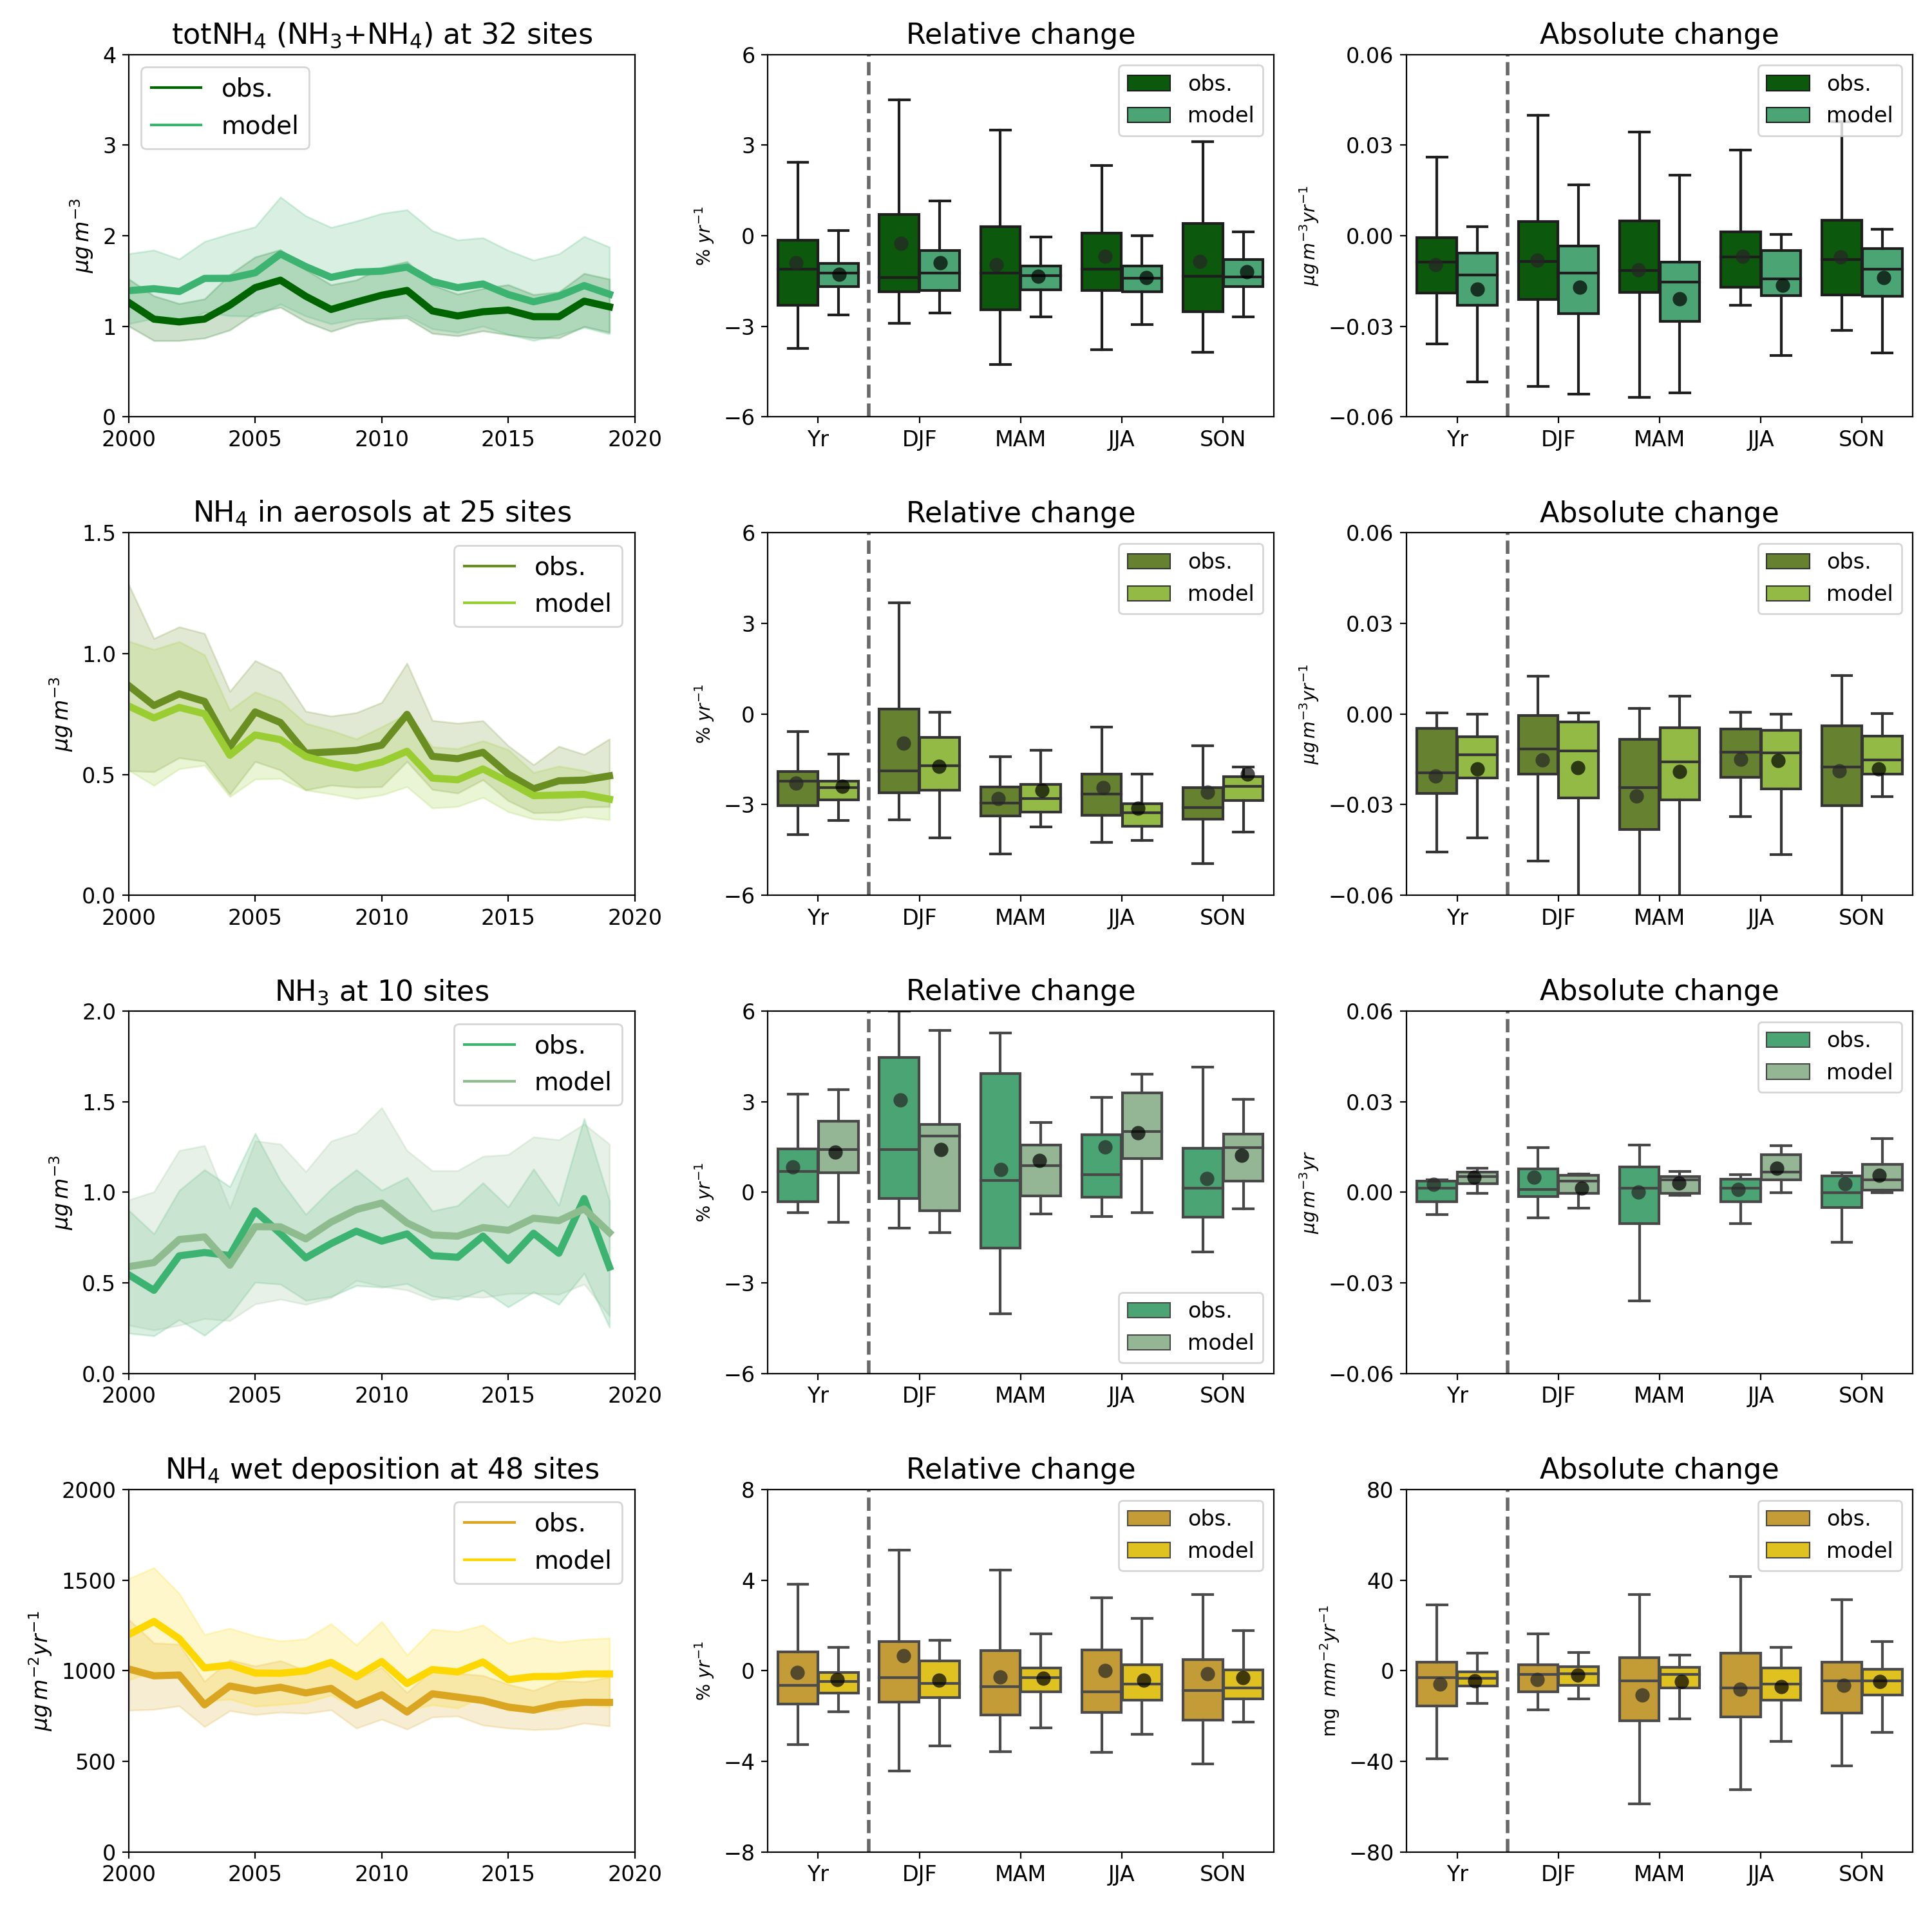
\includegraphics[width=0.74\paperwidth]{FIGS_TRENDS/Nred_trends.png}
	\caption{\label{fig:Nred_trends}Trends in oxidised nitrogen components from 2010-2019 for EMEP observations and model.The solid line in the trend plots indicate the average annual mean concentrations for all the sites and the shaded area the 95 \% confidence interval. The box plot represent the 50,25,75 percentiles and the whiskers lie within the 1.5 inter-quartile ranges for the trends of all the sites, including those with not significant trends. In addition, the mean trends are indicated with black circles and the trend in \nhiii emission is indicated in the plot of total ammonium with secondary y-axes}
\end{figure}

\begin{figure}[h]
  \centering{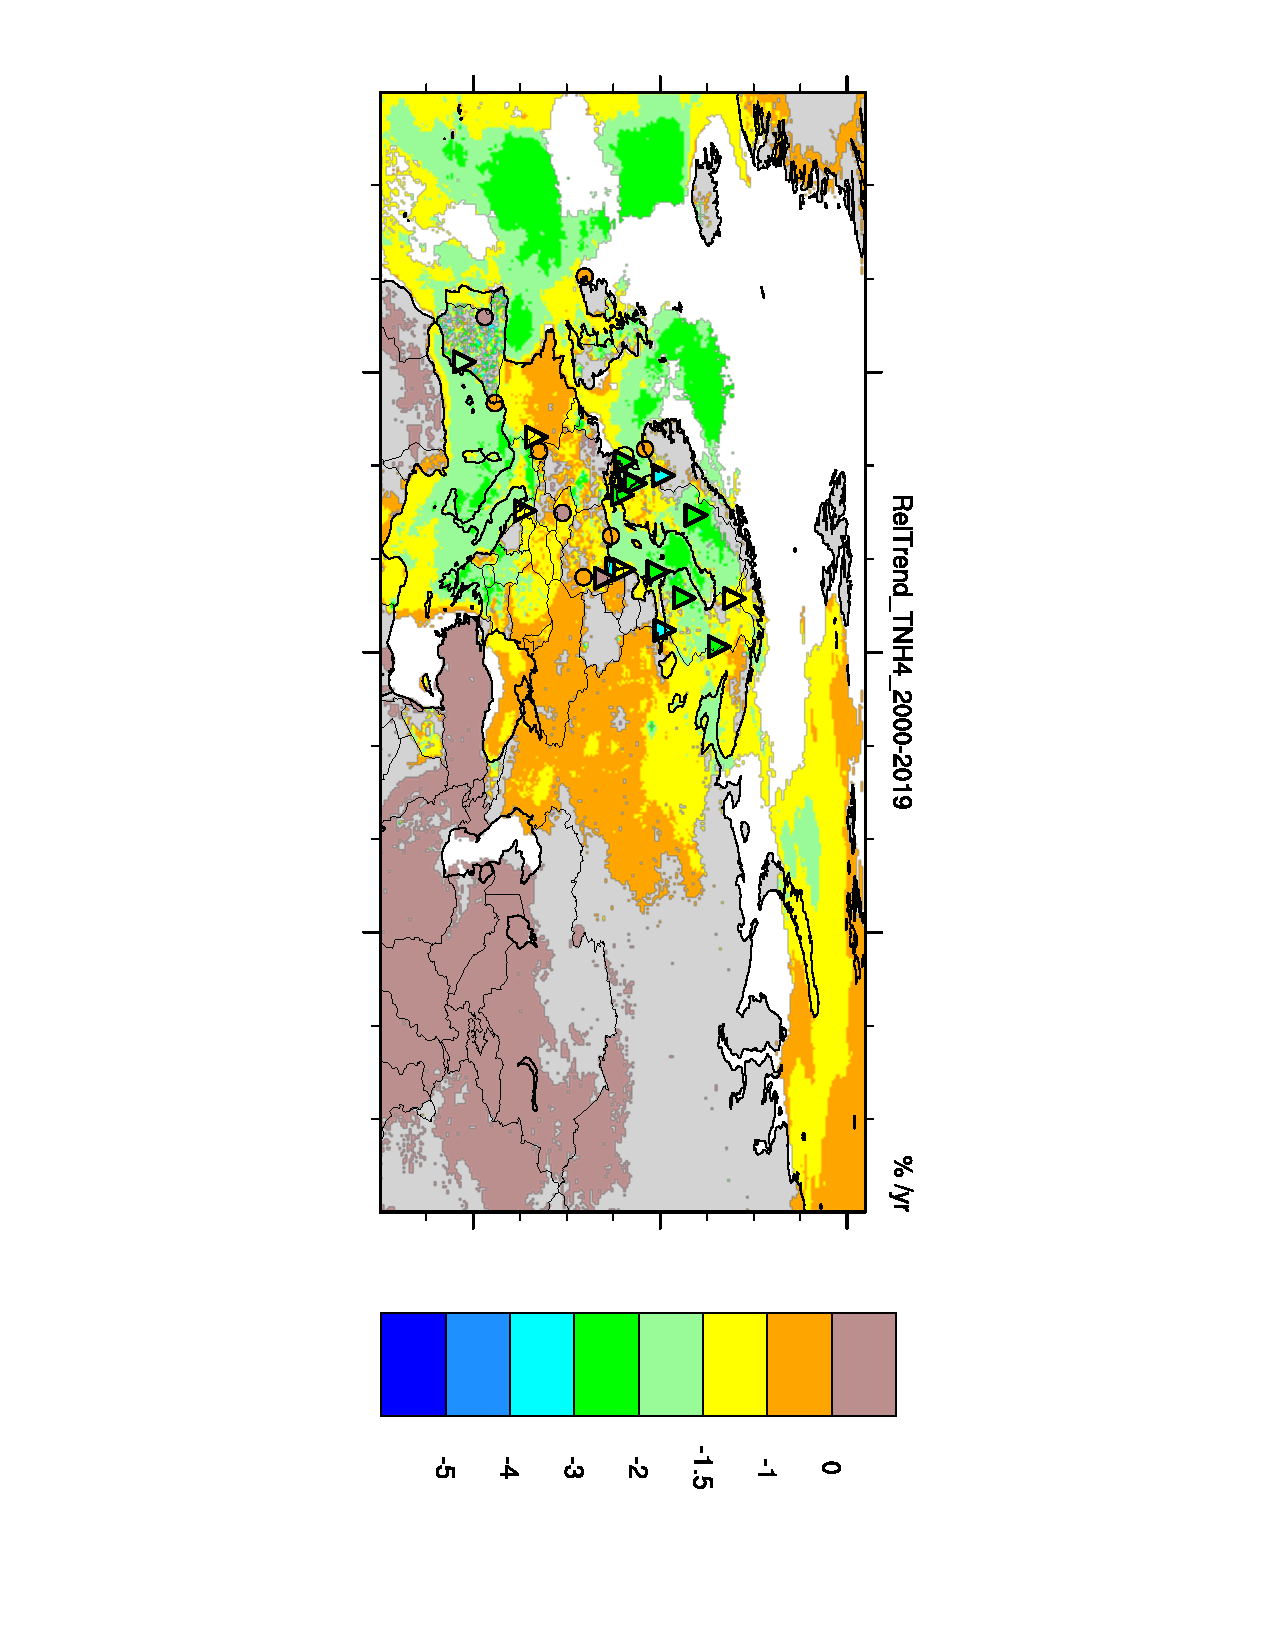
\includegraphics[clip=,angle=90,height=6.1cm,viewport=175 67 448 754]{FIGS_TRENDS/RelTrend_TNH4_2000-2019_Perc.pdf}}
%  \vspace{0.5cm}
  \centering{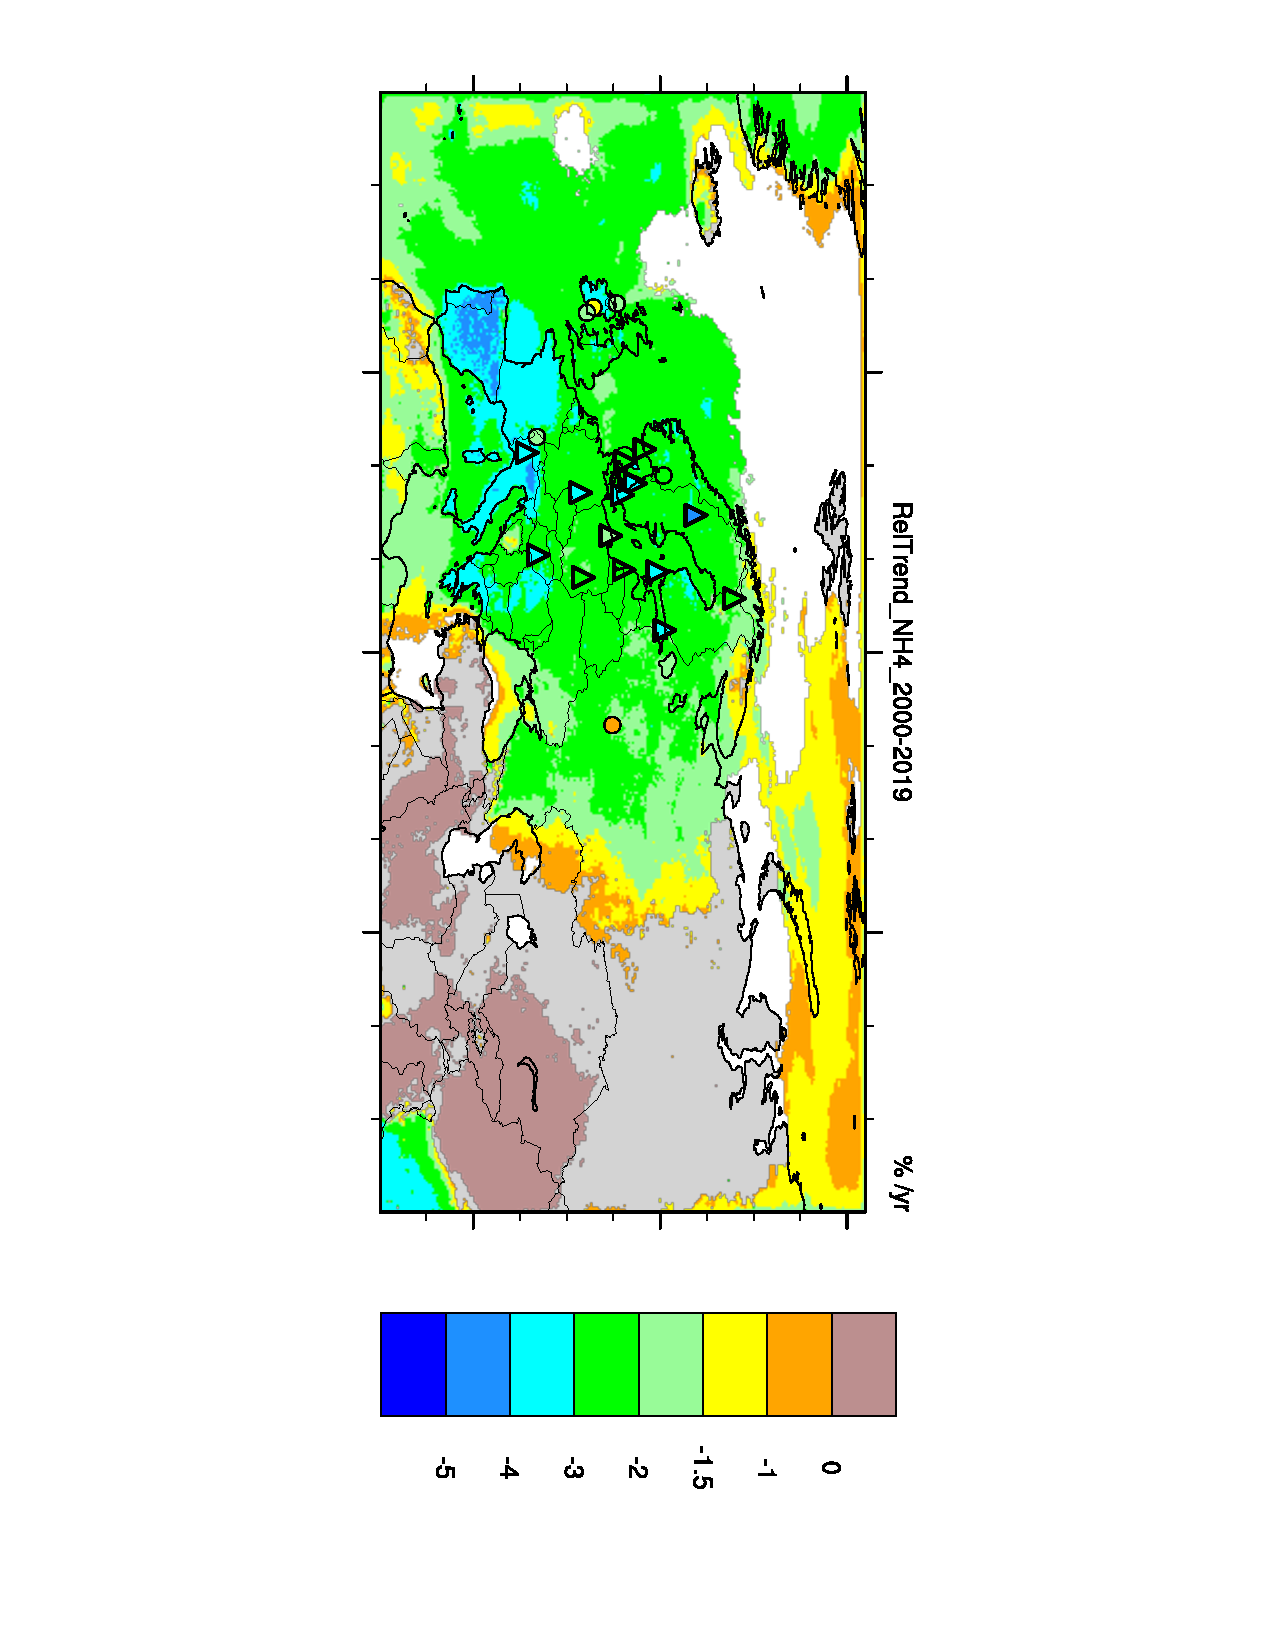
\includegraphics[clip=,angle=90,height=6.1cm,viewport=175 67 448 754]{FIGS_TRENDS/RelTrend_NH4_2000-2019_Perc.pdf}}
\centering{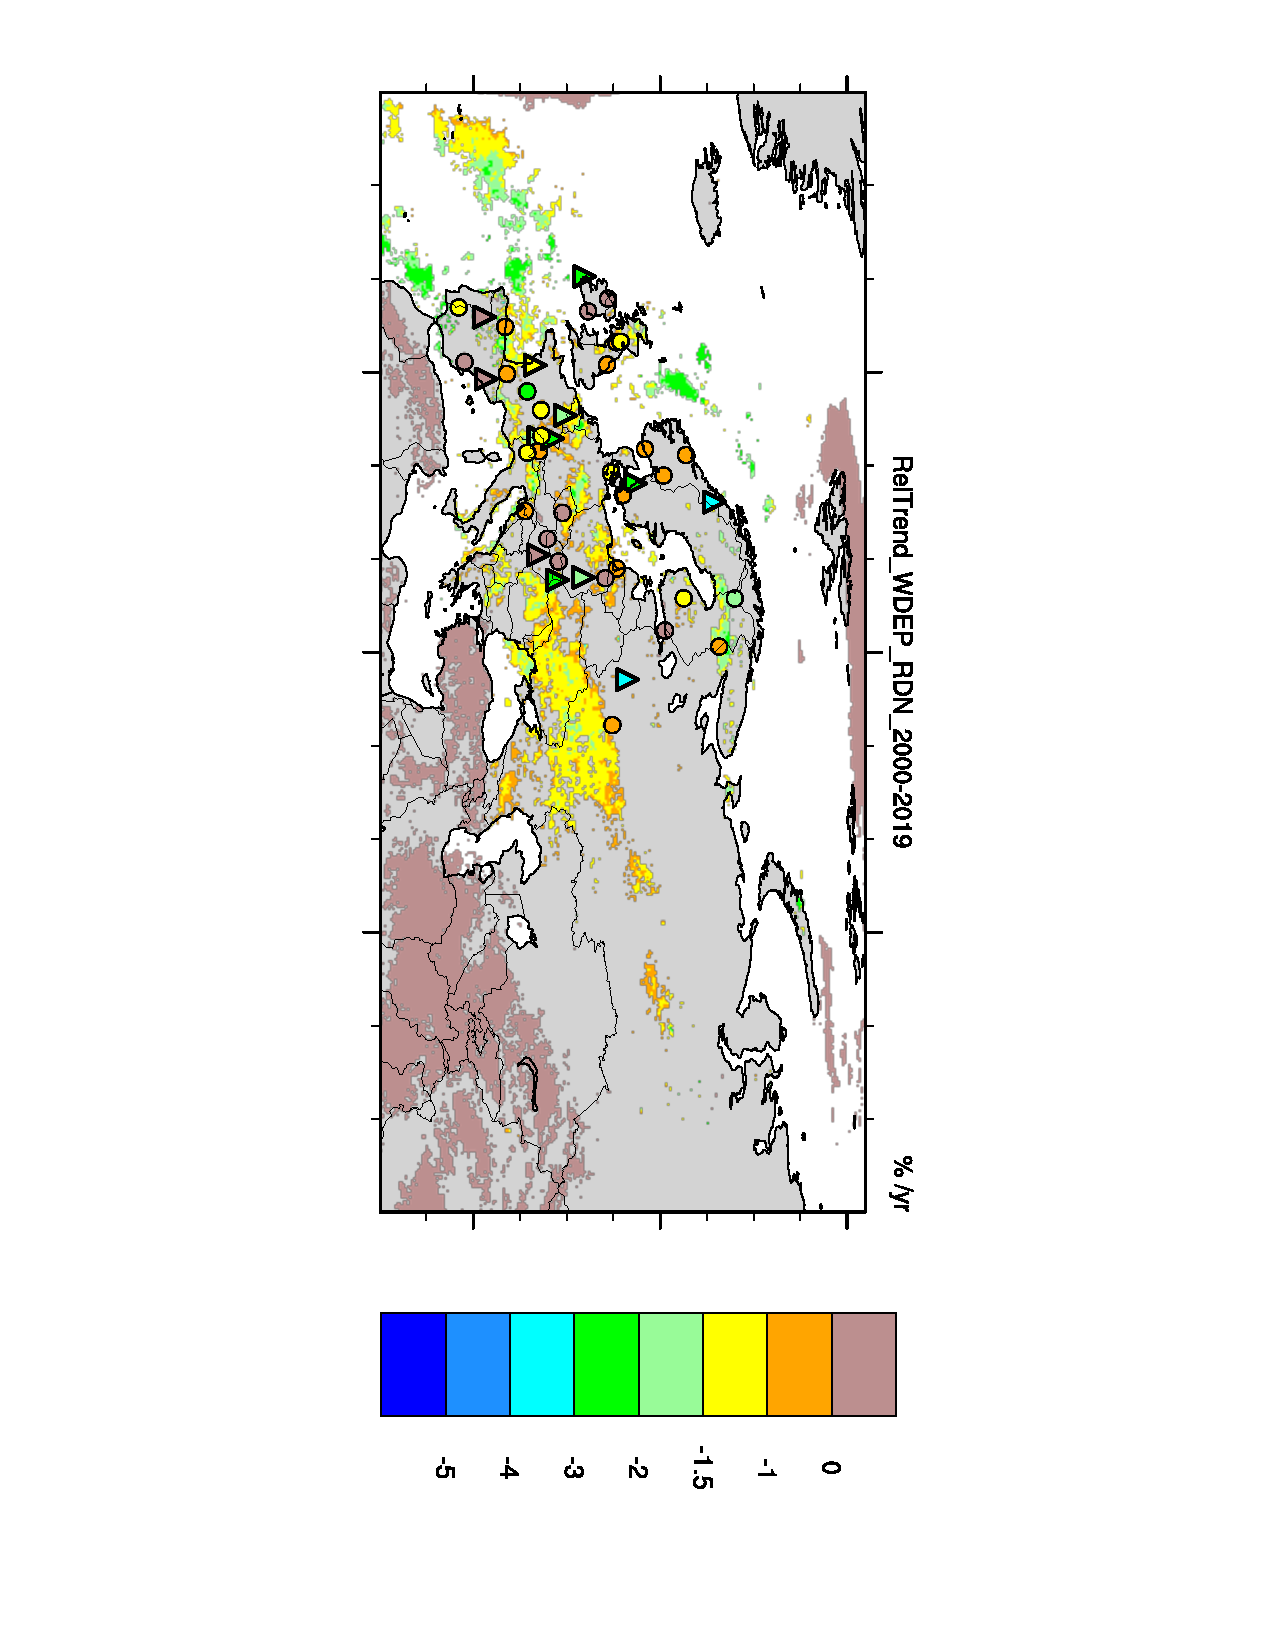
\includegraphics[clip=,angle=90,height=6.1cm,viewport=175 67 448 754]{FIGS_TRENDS/RelTrend_WDEP_RDN_2000-2019_Perc.pdf}}
\caption{Relative trends for total ammonium (sum of ammonia and aerosol ammonium), aerosol ammonium and wet deposition of reduced nitrogen in the period of 2000-2019: EMEP modelled -- coloured contours (grey/white means non-significant trends) and
observed - coloured triangles (significant) and circles (non-significant).}
\label{fig:RDNtrends}
\end{figure}

\begin{table}
\caption{\label{tab:tnh4_stat} Absolute and relative change and corresponding 95\% confidence intervals in observed and modelled annual and seasonal aggregated concentrations of total ammonium (\nhiii+\nhiv) in air and aerosols for the different time periods. The number of sites with a significant outcome is provided.}
\begin{center}
\scalebox{0.65}{%
\begin{tabular}{ll|ccc|cccc|cccc}
\toprule
          &        & \multicolumn{3}{c}{Number of sites} & \multicolumn{4}{c}{Absolute change (\ug $yr^{-1})$} & \multicolumn{4}{c}{Relative change (\% $yr^{-1}$)} \\
Period & Seasons &           total & sign.(obs.) & sign.(mod.) &                    obs. &          conf.interval &  mod. &          conf.interval &                     obs. &         conf.interval &  mod. &        conf.interval \\
\midrule
2000-2019 & all &              25 &          17 &          18 &                  -0.016 &  (-0.024, -0.007) & -0.019 &  (-0.027, -0.012) &                    -1.45 &  (-1.99, -0.91) & -1.36 &  (-1.58, -1.14) \\
          & winter &              28 &           9 &          10 &                  -0.018 &  (-0.029, -0.008) & -0.023 &  (-0.033, -0.013) &                    -1.18 &  (-1.72, -0.64) & -1.14 &  (-1.47, -0.81) \\
          & spring &              25 &          10 &          16 &                  -0.017 &  (-0.029, -0.006) & -0.023 &  (-0.032, -0.015) &                    -1.48 &  (-2.21, -0.75) & -1.46 &   (-1.71, -1.2) \\
          & summer &              25 &          10 &          20 &                  -0.009 &  (-0.018, -0.001) & -0.017 &  (-0.025, -0.009) &                    -1.02 &  (-1.61, -0.44) & -1.44 &  (-1.71, -1.18) \\
          & autumn &              24 &          11 &           7 &                  -0.015 &  (-0.025, -0.006) & -0.016 &  (-0.023, -0.009) &                    -1.67 &  (-2.27, -1.08) & -1.32 &  (-1.61, -1.03) \\
2005-2019 & all &              27 &          12 &          12 &                  -0.019 &  (-0.029, -0.009) & -0.020 &  (-0.029, -0.011) &                    -1.90 &  (-2.55, -1.24) & -1.53 &  (-1.88, -1.18) \\
2010-2019 & all &              27 &           6 &           7 &                  -0.017 &  (-0.026, -0.008) & -0.012 &  (-0.021, -0.004) &                    -2.31 &  (-3.25, -1.36) & -1.12 &   (-1.75, -0.5) \\
2000-2010 & all &              37 &           6 &          13 &                  -0.022 &   (-0.034, -0.01) & -0.024 &  (-0.033, -0.016) &                    -1.36 &  (-2.11, -0.62) & -1.20 &  (-1.82, -0.58) \\
\bottomrule
\end{tabular}}
\end{center}
\end{table}

\begin{table}
\caption{\label{tab:nh4pm_stat} Absolute and relative change and corresponding 95\% confidence intervals in observed and modelled annual and seasonal aggregated concentrations of \nhiv in aerosols for the different time periods.The number of sites with a significant outcome is provided.}
\begin{center}
\scalebox{0.65}{%
\begin{tabular}{ll|ccc|cccc|cccc}
\toprule
          &        & \multicolumn{3}{c}{Number of sites} & \multicolumn{4}{c}{Absolute change (\ug $yr^{-1})$} & \multicolumn{4}{c}{Relative change (\% $yr^{-1}$)} \\
Period & Seasons &           total & sign.(obs.) & sign.(mod.) &                    obs. &          conf.interval &  mod. &          conf.interval &                     obs. &         conf.interval &  mod. &        conf.interval \\
\midrule
2000-2019 & all &              21 &          15 &          20 &                  -0.024 &  (-0.033, -0.016) & -0.021 &  (-0.028, -0.014) &                    -2.61 &  (-3.01, -2.22) & -2.61 &  (-2.79, -2.43) \\
          & winter &              22 &          10 &           9 &                  -0.019 &  (-0.035, -0.002) & -0.020 &  (-0.028, -0.013) &                    -1.47 &  (-2.49, -0.45) & -1.94 &  (-2.43, -1.45) \\
          & spring &              20 &          17 &          16 &                  -0.032 &  (-0.043, -0.021) & -0.022 &   (-0.03, -0.015) &                    -3.09 &  (-3.64, -2.55) & -2.74 &  (-3.17, -2.31) \\
          & summer &              20 &          14 &          20 &                  -0.017 &  (-0.023, -0.012) & -0.018 &  (-0.023, -0.013) &                    -2.78 &  (-3.22, -2.35) & -3.39 &  (-3.62, -3.16) \\
          & autumn &              19 &          11 &          11 &                  -0.023 &  (-0.031, -0.014) & -0.022 &  (-0.032, -0.012) &                    -2.75 &  (-3.65, -1.85) & -2.58 &   (-2.8, -2.35) \\
2005-2019 & all &              27 &          16 &          23 &                  -0.025 &  (-0.033, -0.017) & -0.022 &  (-0.028, -0.016) &                    -2.90 &  (-3.41, -2.38) & -3.01 &   (-3.2, -2.83) \\
2010-2019 & all &              31 &          16 &          17 &                  -0.029 &  (-0.041, -0.017) & -0.019 &  (-0.027, -0.012) &                    -3.48 &   (-4.7, -2.26) & -3.22 &   (-3.9, -2.54) \\
2000-2010 & all &              23 &           9 &          12 &                  -0.034 &   (-0.048, -0.02) & -0.036 &  (-0.047, -0.024) &                    -3.43 &   (-4.6, -2.27) & -3.18 &  (-3.63, -2.73) \\
\bottomrule
\end{tabular}}
\end{center}
\end{table}

\begin{table}
\caption{\label{tab:nh3_stat} Absolute and relative change and corresponding 95\% confidence intervals in observed and modelled annual and seasonal aggregated concentrations of \nhiii for the different time periods. The number of sites with a significant outcome is provided.}
\begin{center}
\scalebox{0.65}{%
\begin{tabular}{ll|ccc|cccc|cccc}
\toprule
          &        & \multicolumn{3}{c}{Number of sites} & \multicolumn{4}{c}{Absolute change (\ug $yr^{-1})$} & \multicolumn{4}{c}{Relative change (\% $yr^{-1}$)} \\
Period & Seasons &           total & sign.(obs.) & sign.(mod.) &                    obs. &          conf.interval &  mod. &          conf.interval &                     obs. &         conf.interval &  mod. &        conf.interval \\
\midrule
2000-2019 & all &               8 &           2 &           6 &                   0.010 &  (-0.005, 0.024) &  0.006 &  (-0.006, 0.017) &                     1.55 &    (0.22, 2.88) &  1.54 &   (0.42, 2.66) \\
          & winter &               8 &           1 &           3 &                   0.007 &  (-0.001, 0.016) &  0.002 &  (-0.007, 0.011) &                     4.03 &    (0.61, 7.44) &  1.47 &    (0.1, 2.84) \\
          & spring &               8 &           3 &           3 &                   0.011 &   (-0.007, 0.03) &  0.003 &  (-0.005, 0.011) &                     1.76 &   (-0.32, 3.83) &  1.46 &   (0.09, 2.84) \\
          & summer &               8 &           1 &           6 &                   0.013 &  (-0.009, 0.035) &  0.009 &   (-0.002, 0.02) &                     2.53 &    (-0.3, 5.36) &  2.27 &   (0.88, 3.65) \\
          & autumn &               8 &           1 &           4 &                   0.008 &   (-0.005, 0.02) &  0.007 &  (-0.001, 0.015) &                     0.94 &   (-0.36, 2.24) &  1.49 &   (0.65, 2.33) \\
2005-2019 & all &              18 &           3 &           7 &                   0.005 &  (-0.002, 0.012) &  0.000 &   (-0.009, 0.01) &                     0.57 &   (-0.26, 1.39) &  0.84 &    (0.1, 1.59) \\
2010-2019 & all &              22 &           4 &           5 &                   0.012 &  (-0.009, 0.032) &  0.001 &  (-0.017, 0.019) &                     2.80 &   (-1.35, 6.95) &  2.58 &   (0.67, 4.49) \\
2000-2010 & all &              12 &           3 &           4 &                   0.003 &  (-0.021, 0.028) &  0.012 &     (0.0, 0.025) &                     3.14 &     (0.5, 5.78) &  1.99 &    (0.4, 3.57) \\
\bottomrule
\end{tabular}}
\end{center}
\end{table}

\begin{table}
\caption{\label{tab:nh4dep_stat} Absolute and relative change and corresponding 95\% confidence intervals in observed and modelled annual and seasonal aggregated data of wet deposition of ammonium for the different time periods. The number of sites with a significant outcome is provided.}
\begin{center}
\scalebox{0.7}{%
\begin{tabular}{ll|ccc|cccc|cccc}
\toprule
          &        & \multicolumn{3}{c}{Number of sites} & \multicolumn{4}{c}{Average change (\ugN $m^{2} yr^{-1}$)} & \multicolumn{4}{c}{Relative change (\% $yr^{-1}$)} \\
Period & Seasons &           total & sign.(obs.) & sign.(mod.) &                    obs. &          conf.interval &  mod. &          conf.interval &                     obs. &         conf.interval &  mod. &        conf.interval \\
\midrule
2000-2019 & all &              44 &          13 &           9 &                    -7.4 &  (-11.8, -3.0) &  -4.8 &   (-8.1, -1.5) &                    -0.31 &   (-0.99, 0.37) & -0.40 &  (-0.71, -0.09) \\
          & winter &              44 &           5 &           3 &                    -5.3 &   (-9.4, -1.3) &  -1.7 &    (-3.8, 0.4) &                    -0.25 &   (-0.94, 0.43) & -0.39 &  (-0.72, -0.06) \\
          & spring &              42 &           5 &           4 &                   -12.2 &  (-19.4, -4.9) &  -4.7 &   (-11.5, 2.1) &                    -0.39 &    (-1.1, 0.31) & -0.27 &   (-0.64, 0.11) \\
          & summer &              43 &           9 &           6 &                   -10.4 &  (-16.7, -4.1) &  -8.0 &  (-11.6, -4.4) &                    -0.12 &   (-1.17, 0.93) & -0.48 &  (-0.84, -0.12) \\
          & autumn &              43 &          10 &           4 &                    -7.5 &  (-12.8, -2.3) &  -5.2 &   (-9.3, -1.0) &                    -0.45 &   (-1.37, 0.47) & -0.35 &    (-0.8, 0.11) \\
2005-2019 & all &              52 &           8 &           4 &                    -4.8 &   (-10.7, 1.0) &  -3.4 &   (-6.4, -0.3) &                    -0.12 &   (-0.95, 0.71) & -0.43 &  (-0.78, -0.08) \\
2010-2019 & all &              62 &           3 &           4 &                    -2.7 &    (-8.6, 3.1) &  -5.8 &  (-11.1, -0.4) &                     0.90 &   (-0.95, 2.75) & -0.47 &   (-1.04, 0.11) \\
2000-2010 & all &              44 &           4 &           3 &                    -9.3 &  (-17.8, -0.8) &  -4.0 &   (-12.2, 4.2) &                    -0.36 &   (-1.24, 0.52) & -0.09 &   (-0.91, 0.73) \\
\bottomrule
\end{tabular}}
\end{center}
\end{table}



\section{\label{sec:Trends_PM }Trends in \PM[10] and \PM[2.5] }

Figure~\ref{fig:pm_trends} shows an overview of the annual and seasonal observed and modelled trends in \PM[10] and \PM[2.5] in the period of 2000 to 2019. Tables \ref{tab:pm10_stat} and \ref{tab:pm25_stat} provide further information regarding observed and modelled trends, i.e. the number of sites considered and those with significant trends, the average absolute and relative trends (including confidence intervals) for the 2000-2019 period, for 2000-2010 and 2010-2019 sub-periods, and also for 2005-2019.


\begin{figure}
	\centering
	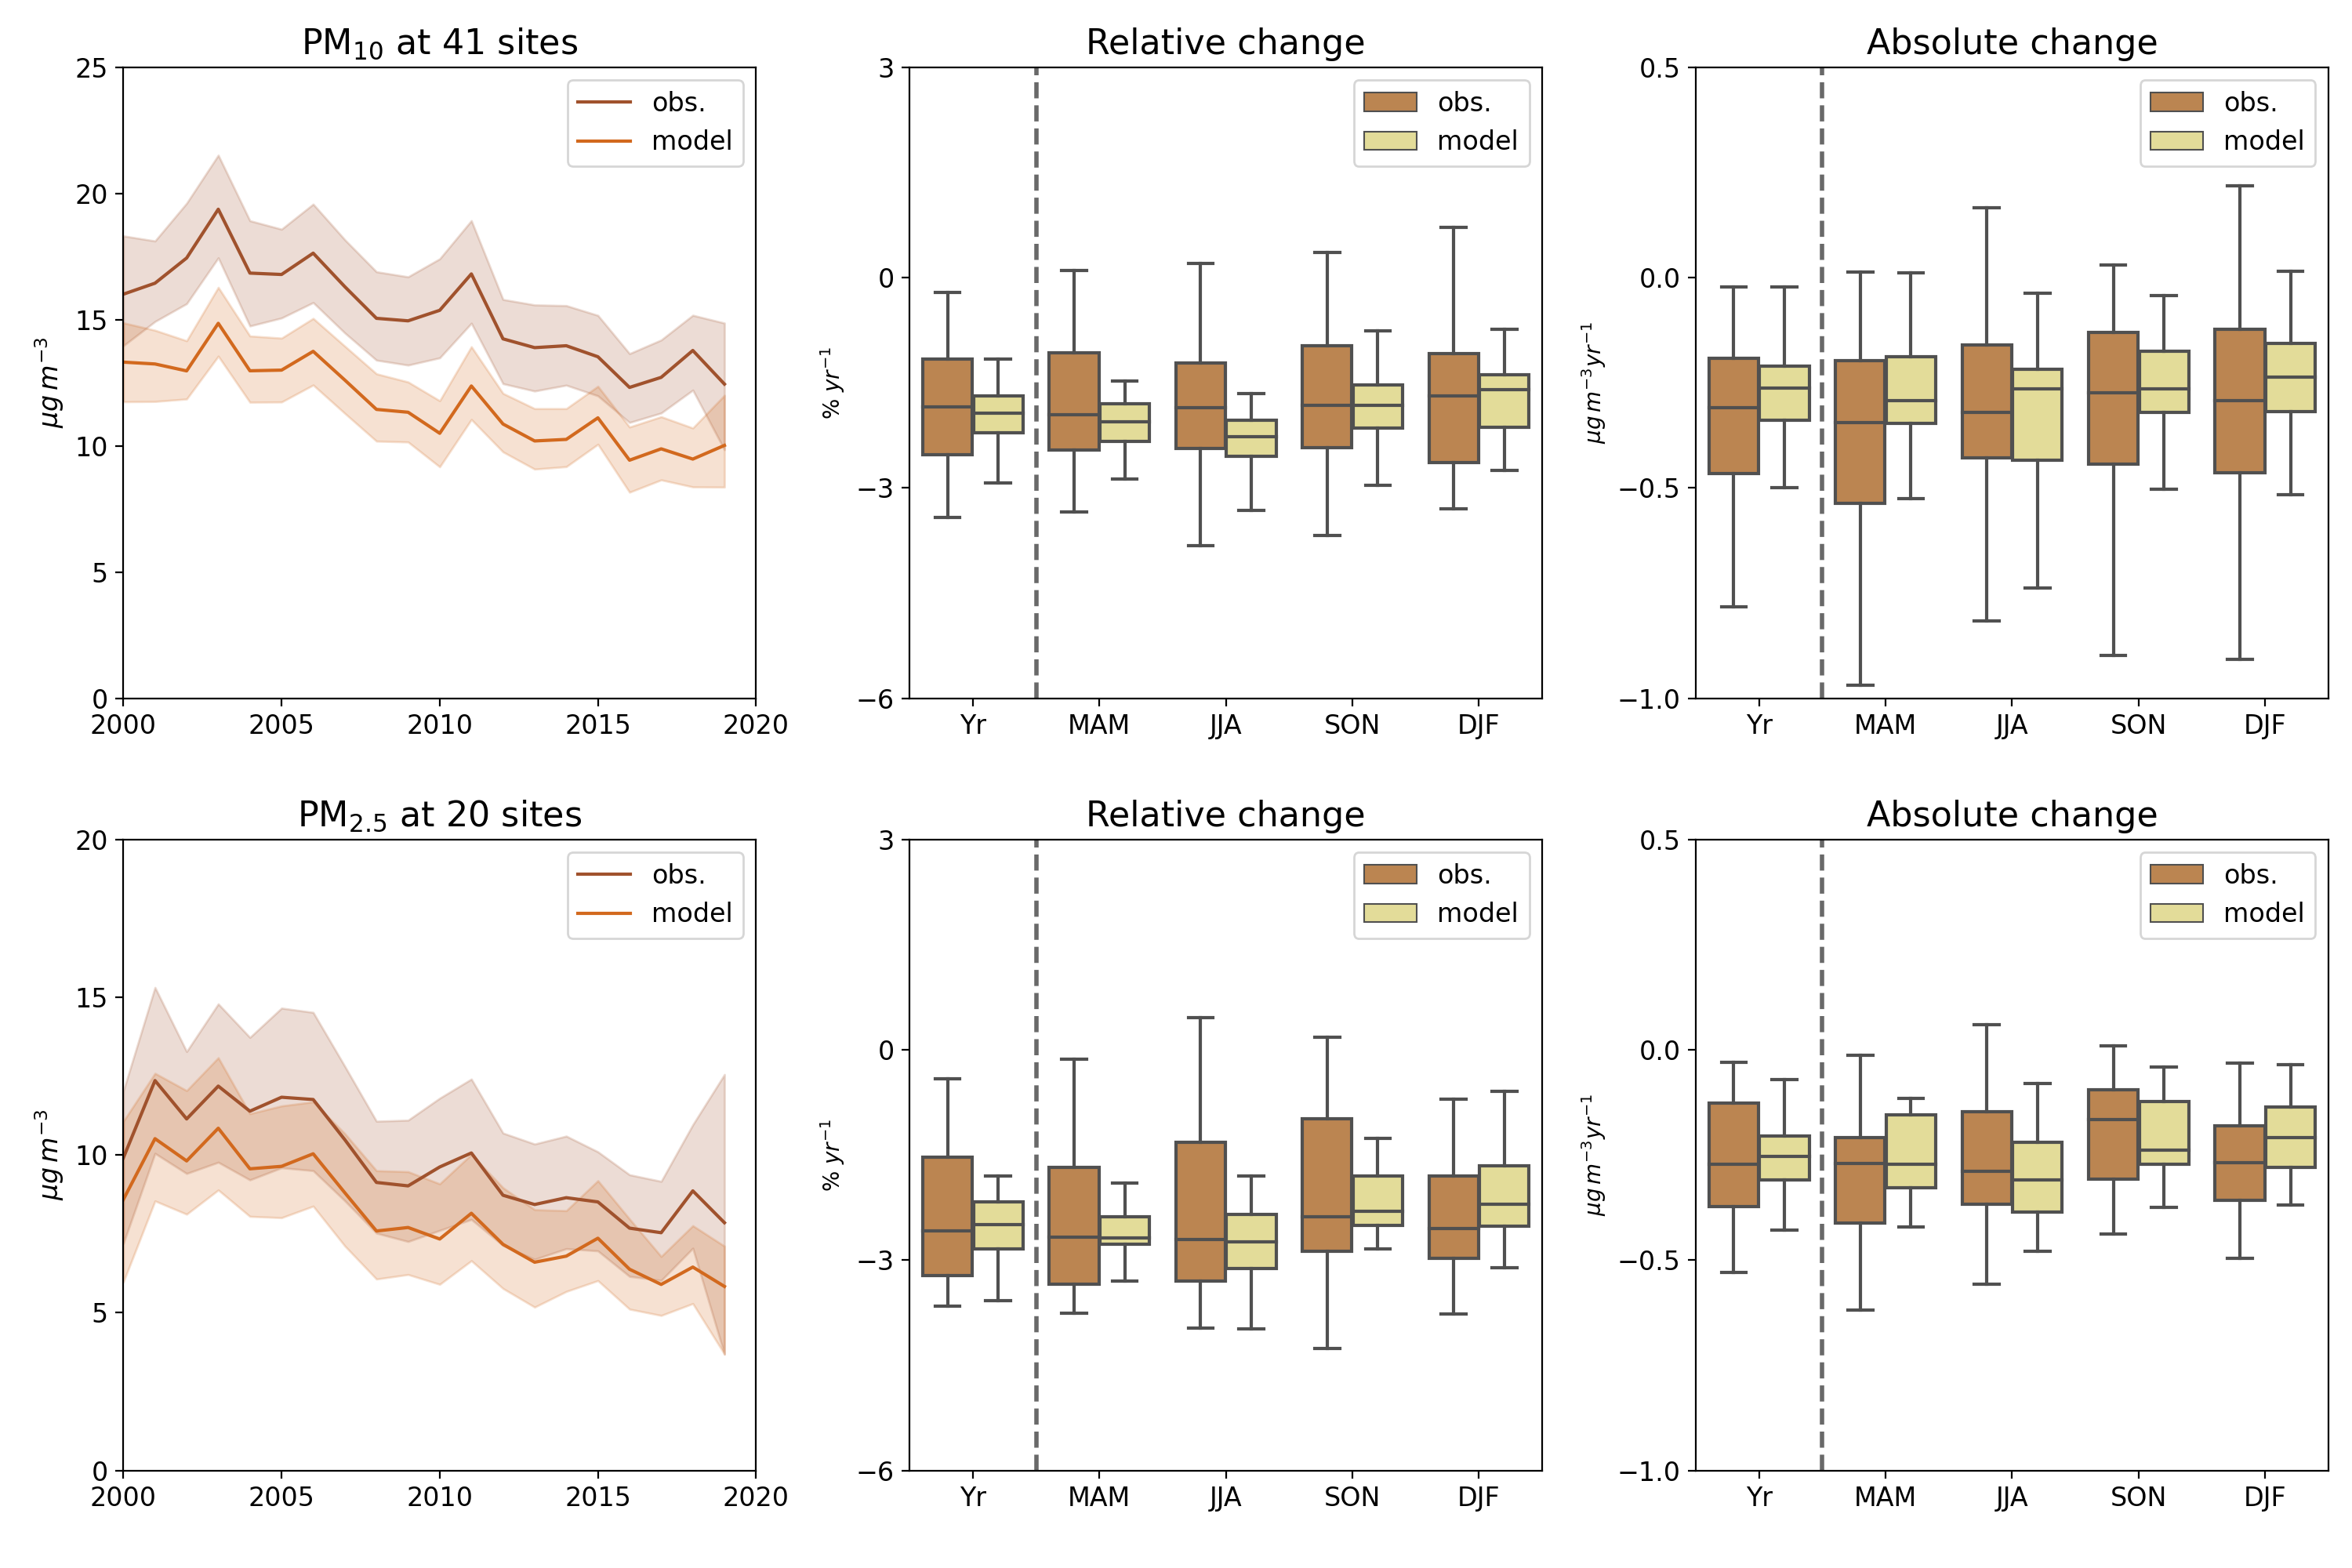
\includegraphics[width=0.74\paperwidth]{FIGS_TRENDS/PM_trends.png}
	\caption{\label{fig:pm_trends}Trends in \PM[10]  and \PM[2.5] from 2010-2019 for EMEP observations and model: left panels - annual timeseries (the solid line indicates the average annual mean trend for all sites, the shaded area shows the 95 \% confidence interval); middle and right panels - relative and absolute trends for all the sites, with both significant and not significant trends (the boxes represent the 50,25,75 percentiles, the whiskers lie within the 1.5 inter-quartile ranges, the mean trends are indicated with black circles}
\end{figure}


\begin{table}
\caption{\label{tab:pm10_stat} Absolute and relative change and corresponding 95\% confidence intervals in observed and modelled annual and seasonal aggregated concentration of \PM[10] for the different time periods. The number of sites with a significant outcome is provided.}
\begin{center}
\scalebox{0.65}{%
\begin{tabular}{ll|ccc|cccc|cccc}
\toprule
          &        & \multicolumn{3}{c}{Number of sites} & \multicolumn{4}{c}{Absolute change (\ug $yr^{-1})$} & \multicolumn{4}{c}{Relative change (\% $yr^{-1}$)} \\
Period & Seasons &           total & sign.(obs.) & sign.(mod.) &                    obs. &          conf.interval &  mod. &          conf.interval &                     obs. &         conf.interval &  mod. &        conf.interval \\
\midrule
2000-2019 & all &              37 &          29 &          36 &                   -0.36 &  (-0.43, -0.29) & -0.29 &  (-0.32, -0.25) &                    -1.83 &  (-2.09, -1.57) & -1.95 &  (-2.11, -1.79) \\
          & winter &              34 &          18 &          20 &                   -0.36 &  (-0.47, -0.25) & -0.26 &  (-0.31, -0.21) &                    -1.73 &   (-2.07, -1.4) & -1.64 &  (-1.83, -1.45) \\
          & spring &              34 &          24 &          32 &                   -0.39 &  (-0.47, -0.31) & -0.30 &  (-0.35, -0.25) &                    -1.84 &  (-2.11, -1.56) & -2.10 &   (-2.29, -1.9) \\
          & summer &              36 &          27 &          31 &                   -0.34 &  (-0.42, -0.25) & -0.32 &  (-0.37, -0.26) &                    -1.72 &  (-2.09, -1.35) & -2.25 &  (-2.47, -2.03) \\
          & autumn &              35 &          22 &          29 &                   -0.34 &  (-0.42, -0.26) & -0.30 &  (-0.34, -0.26) &                    -1.81 &   (-2.1, -1.51) & -1.91 &  (-2.09, -1.74) \\
2005-2019 & all &              54 &          29 &          38 &                   -0.33 &  (-0.41, -0.25) & -0.23 &  (-0.27, -0.19) &                    -1.82 &  (-2.23, -1.41) & -1.79 &  (-2.07, -1.51) \\
2010-2019 & all &              56 &          17 &          23 &                   -0.32 &  (-0.42, -0.21) & -0.16 &  (-0.21, -0.11) &                    -1.84 &  (-2.45, -1.23) & -1.38 &  (-1.81, -0.95) \\
2000-2010 & all &              36 &          14 &          24 &                   -0.46 &  (-0.56, -0.36) & -0.35 &  (-0.46, -0.24) &                    -2.36 &  (-2.77, -1.95) & -2.40 &  (-2.97, -1.83) \\
\bottomrule
\end{tabular}}
\end{center}
\end{table}


\begin{table}
\caption{\label{tab:pm25_stat} Absolute and relative change and corresponding 95\% confidence intervals in observed and modelled annual and seasonal aggregated concentration of \PM[25] for the different time periods. The number of sites with a significant outcome is provided.}
\begin{center}
\scalebox{0.65}{%
\begin{tabular}{ll|ccc|cccc|cccc}
\toprule
          &        & \multicolumn{3}{c}{Number of sites} & \multicolumn{4}{c}{Absolute change (\ug $yr^{-1})$} & \multicolumn{4}{c}{Relative change (\% $yr^{-1}$)} \\
Period & Seasons &           total & sign.(obs.) & sign.(mod.) &                    obs. &          conf.interval &  mod. &          conf.interval &                     obs. &         conf.interval &  mod. &        conf.interval \\
\midrule
2000-2019 & all &              19 &          16 &          19 &                   -0.29 &   (-0.39, -0.2) & -0.26 &  (-0.31, -0.22) &                    -2.42 &   (-2.84, -2.0) & -2.52 &  (-2.71, -2.32) \\
          & winter &              18 &          12 &          12 &                   -0.36 &  (-0.54, -0.18) & -0.21 &  (-0.25, -0.17) &                    -2.29 &  (-2.74, -1.85) & -2.08 &  (-2.35, -1.82) \\
          & spring &              19 &          14 &          19 &                   -0.32 &  (-0.41, -0.24) & -0.27 &  (-0.31, -0.22) &                    -2.47 &  (-2.91, -2.03) & -2.69 &  (-2.88, -2.51) \\
          & summer &              18 &          14 &          17 &                   -0.26 &  (-0.33, -0.19) & -0.30 &  (-0.36, -0.23) &                    -2.36 &  (-2.91, -1.82) & -2.81 &  (-3.16, -2.47) \\
          & autumn &              18 &          12 &          16 &                   -0.26 &  (-0.36, -0.15) & -0.26 &  (-0.33, -0.18) &                    -2.22 &  (-2.71, -1.74) & -2.29 &   (-2.5, -2.07) \\
2005-2019 & all &              36 &          23 &          28 &                   -0.33 &  (-0.42, -0.23) & -0.21 &  (-0.25, -0.17) &                    -2.66 &  (-3.16, -2.16) & -2.28 &  (-2.55, -2.01) \\
2010-2019 & all &              43 &          20 &          19 &                   -0.34 &  (-0.43, -0.25) & -0.18 &  (-0.23, -0.13) &                    -3.14 &   (-3.7, -2.57) & -2.21 &  (-2.67, -1.74) \\
2000-2010 & all &              20 &           7 &          12 &                   -0.36 &   (-0.5, -0.21) & -0.36 &  (-0.46, -0.26) &                    -2.65 &  (-3.56, -1.73) & -2.93 &  (-3.58, -2.27) \\

\bottomrule
\end{tabular}}
\end{center}
\end{table}



\begin{figure}  %DS[H]
  \centering{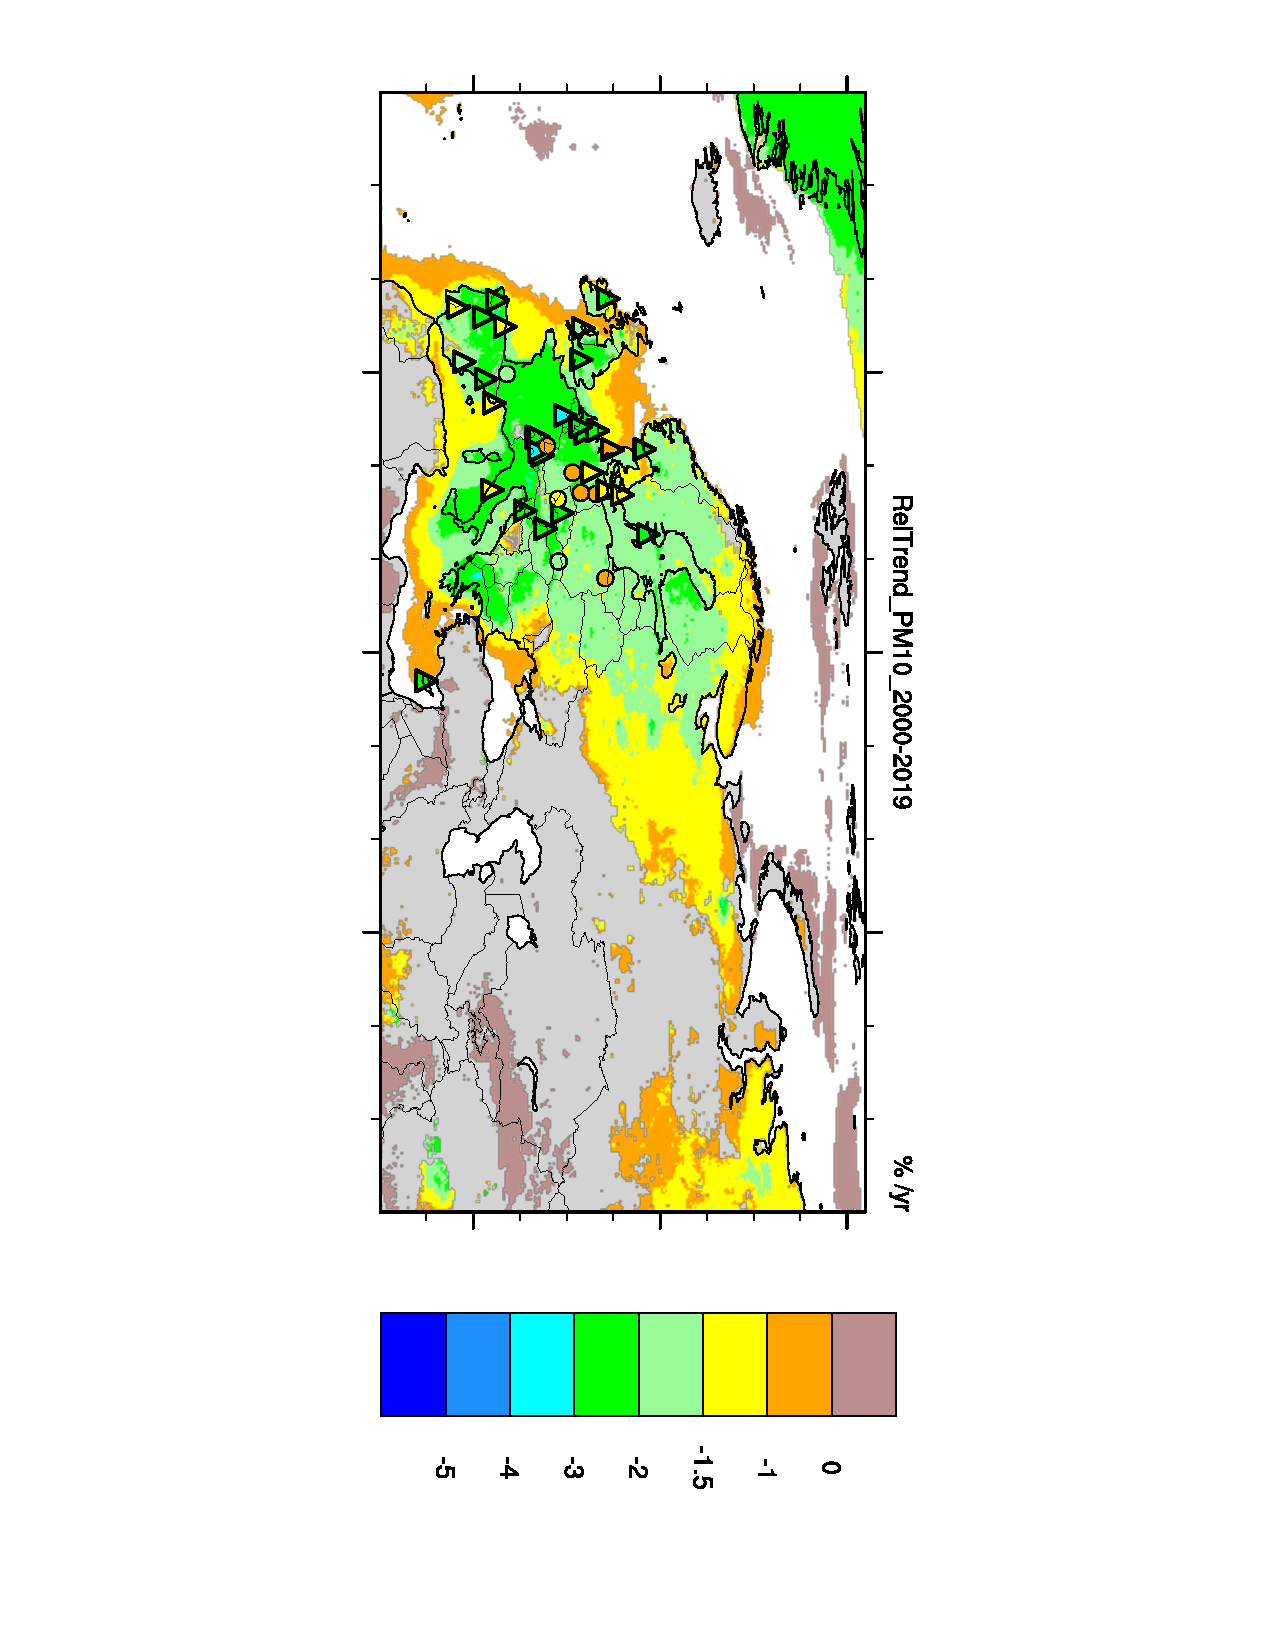
\includegraphics[clip=,angle=90,height=6.1cm,viewport=175 67 448 754]{FIGS_TRENDS/RelTrend_PM10_2000-2019_Perc.pdf}}\\
%  \vspace{0.5cm}
  \centering{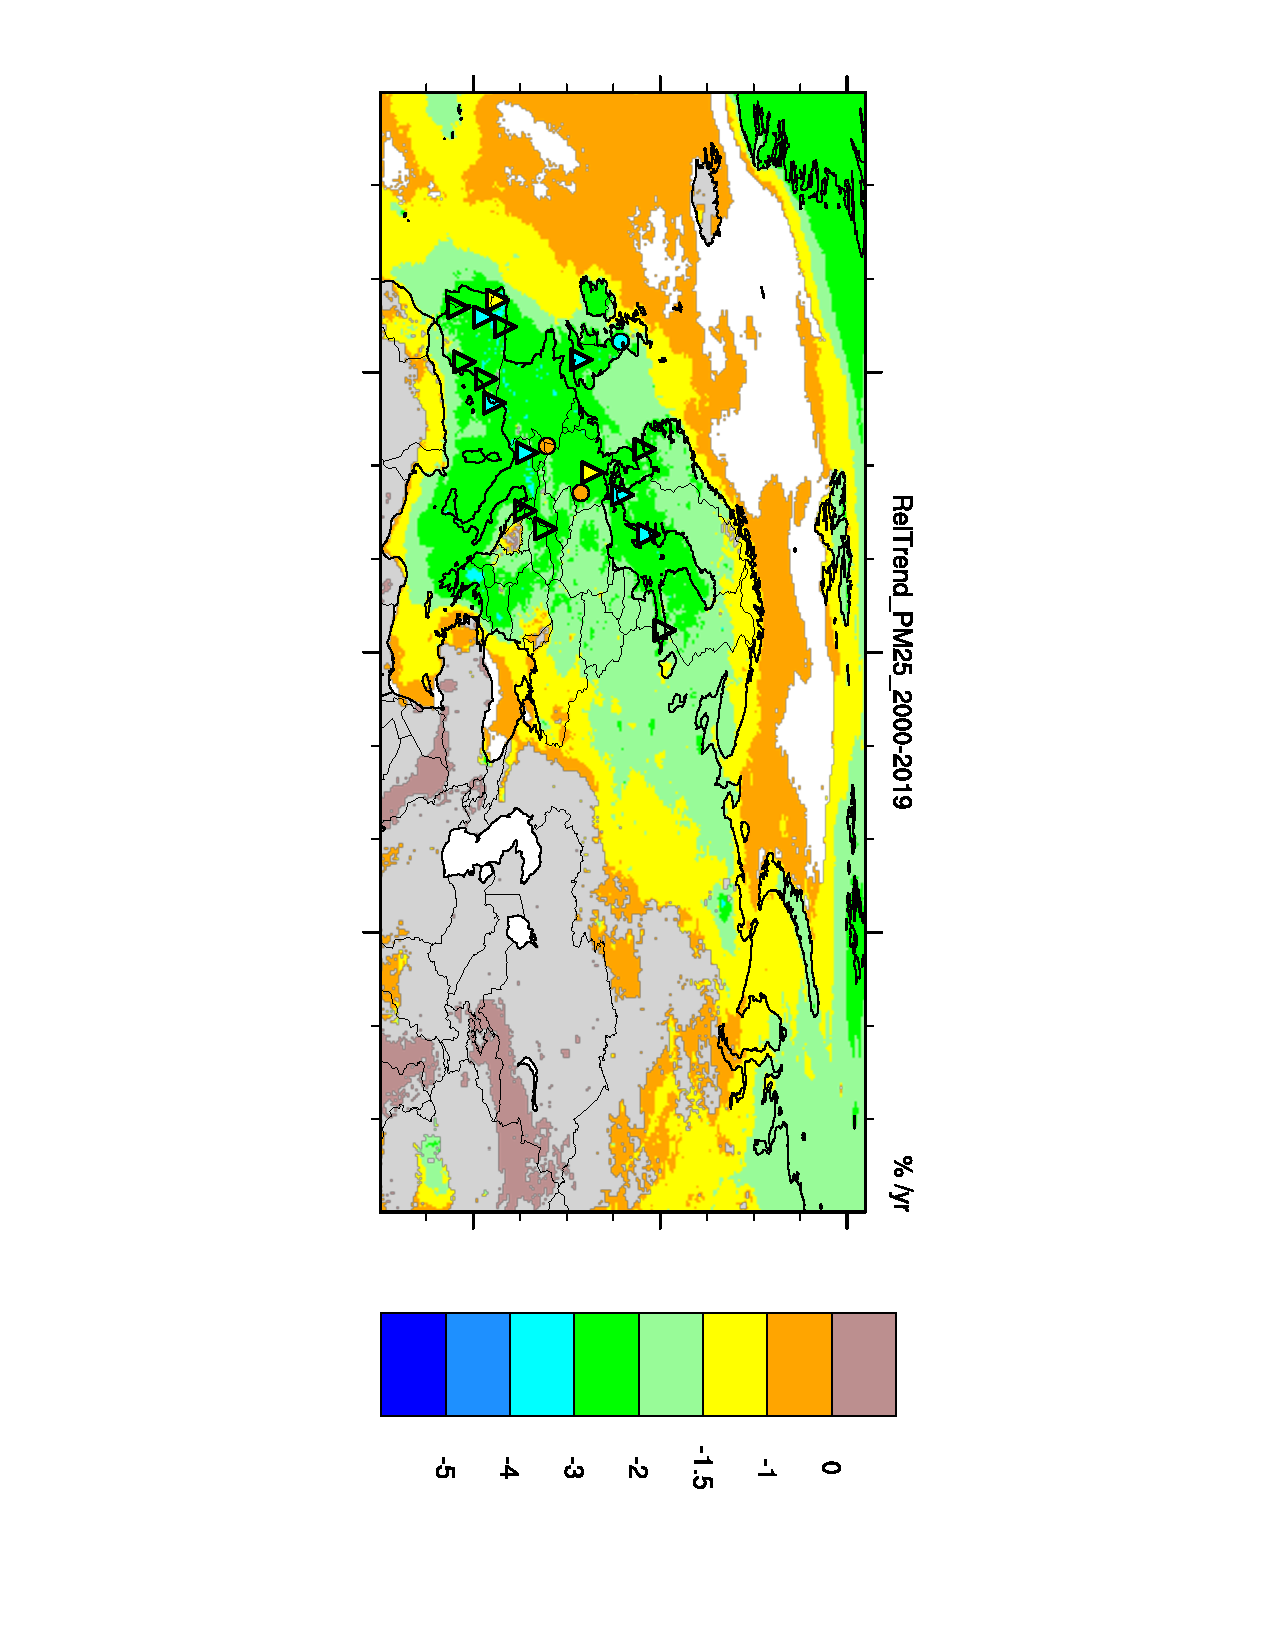
\includegraphics[clip=,angle=90,height=6.1cm,viewport=175 67 448 754]{FIGS_TRENDS/RelTrend_PM25_2000-2019_Perc.pdf}}
\caption{Relative trends for \PM[10] and \PM[2.5] in the period of 2000-2019: EMEP modelled -- coloured contours (grey/white means non-significant trends) and observed - coloured triangles (significant) and circles (non-significant).}
\label{fig:PMtrends}
\end{figure}


For the whole period, 36 and 18 sites with satisfactory data coverage have been included in the trend analysis respectively for \PM[10] and \PM[2.5]. The annual series of \PM[10] and \PM[2.5] clearly show a general concentration decrease from 2000 to 2019. In general, the model underestimates the concentrations, but reproduces quite well observed year-to-year changes in \PM[10] and \PM[2.5], including enhanced PM levels due to meteorological conditions e.g. in 2003 (dry hot summer \citep{EMEP:PM2005}) and 2011 (dry year in Western/Central/Southern Europe \citep{EMEP:PM2013}).


For the period of 2000-2019, the average observed \PM[10] trends are -0.36 \ug $yr^{-1}$, or -1.83 \% $yr^{-1}$ in relative terms. The corresponding \PM[10] trends from model simulations are -0.27 \ug $yr^{-1}$ and -1.92 \% $yr^{-1}$. For \PM[2.5], the average absolute trends are -0.29 and -0.25 \ug $yr^{-1}$ and the relative ones are -2.42 and -2.51 \% $yr^{-1}$, observed and modelled respectively. The reduction of anthropogenic emissions during this period is a major cause for the decreasing average concentrations of PM, with \PM[10] trends experiencing larger disturbances due to considerable contribution from natural aerosols of sea salt and mineral dust in the coarse fraction. Considerable changes in PM pollution caused by the inter-annual meteorological variability also interfere with the PM trends due to emission changes, as the weather conditions affect both the formation of secondary aerosols, emissions of natural particles, and dry and wet depositions.


Figure \ref{fig:pm_trends} reveals a considerably larger variation of observed trends between the sites in comparison to modelled trends, still with modelled median (and mean) trends lying within 25-75\% inter-quartile range (IQR) of the observed ones. A larger spatial variability of observed trends with respect to model simulated ones can also be seen on the maps of relative trends in Figure \ref{fig:pm_trends}. The largest decreases in \PM[10] were observed at the French site (FR0009) by 3.4 \% $yr^{-1}$ and at the Swiss (CH0005) by 3.1 \% $yr^{-1}$. and the smallest, below 1\%, in Germany and Poland. For \PM[2.5], decrease larger than -3 \% $yr^{-1}$ was observed at 8 out of 19 sites, situated in Sweden, Norway, the UK, Spain, the Po Valley, and in Austria, while the smallest decreasing trends were as for \PM[10] registered at German sites. The modelled \PM[10] and \PM[2.5] trends are between -1.5 and -2.5 \% $yr^{-1}$ for most of Europe (with the largest decrease of \PM[2.5] between -2.5 and -3 \% $yr^{-1}$ in France). Most of the sites, for which the observations estimate insignificant trends, are located in Central Europe (mostly in Germany). The modelled trends are mostly significant and ranging between -1 and -3 \% over practically all European part of EMEP.

The observations and model simulations indicate more sites with significant trends and larger \PM[10] and \PM[2.5] average decreases for the warm seasons. For the cold seasons, when PM pollution is typically more serious, the relative decreasing trends are in general smaller, and the number of sites with non-significant trends is larger, which is especially pronounced for observed \PM[10] trends.

PM is a complex pollutant, consisting of aerosol species both emitted
directly and formed from gaseous precursors.Therefore, the reductions both in primary PM emissions, as well as \sox, \noii, \nhiii and NMVOC emissions are contribute to decrease PM concentrations. In the western parts of EMEP (EU \&UK \&EFTA), where the considered sites are located, the emissions of primary \PM[10] and \PM[2.5] were reduced by 32 and 35 \%, respectively, from 2000 to 2019. The largest in the same period was the reduction in \sox emissions (81 \%), resulting in 61 \% observed decrease of \soiv (70 \% according to the model). Following the reduction of \noii emissions by 48 \%, observed \noiii concentrations decreased slightly less, i.e. by 38 \% (44 \% according to the model). This was partly due to a rather moderate reduction by 12 \% in \nhiii emissions and the availability of free \nhiii due to the reduced formation of ammonium sulphate. 

\COMMENT{Though \noii was reduced by 48 \%, given the moderate reduction by 12 \% in \nhiii emissions and the availability of free \nhiii due to the reduced formation of ammonium sulphate, the observed decrease in \noiii concentrations was only 38 \% (44 \% by the model).}
 The corresponding changes from 2000 to 2019 in \nhiv were 50 and 48 \%. Due to the lack of consistent observational data for carbonaceous aerosols in the 2000s, the trends of elemental (EC) and organic (OC) carbon have only been analysed for a 2010-2019 period (see discussion in \ref{sec:trendsECOC}). The examples of the changes in the chemical composition of \PM[2.5] from 2000(2002) to 2019 are given on Figure \ref{fig:KEX4} for the only six sites with enough measurements for deriving the mass balance. 

Summarizing trend results for the 2000-2019 period, the average \PM[10] and \PM[2.5] trends, derived from observational data and model simulations, are decreasing. Significant trends have been estimated from observational data for 78 \% of sites for \PM[10] and 84 \% of sites for \PM[2.5]; the model simulates significant trends for more sites, namely 97 and 100 \% respectively. During this 20-year period, observed \PM[10] concentrations decreased by 35 \%  (36 \% from model simulations) on average at the considered sites. The average observed decrease of \PM[2.5] is 46 \%  (48 \% estimated by the model). We find quite a good correspondence between observed and model simulated trends in PM concentrations. 

\COMMENT{For the period 2005-2019 (starting from the reference year of Gothenburg Protocol), more sites with data coverage were totally available for this \PM[10] and \PM[2.5] trend analysis, i.e. 53 and 35 respectively, but significant trends have been observed and modelled for a smaller fraction of the sites with respect to the 2000-2019 period (partly due to a shorter period length)}


%%%%%%%%%%%%%%%%%%%%%%%%%%%%%%%%%%%%%%%%%%%%%%%%%%%%%%%%%%%%%%%%%%%%%%%%%%%%%%%%%%%%%%%%%%%%%%%%%%%%%%%%
\clearpage
\section{\label{sec:Trends_O3}Trends in O$_3$ }

Trend studies of surface ozone requires a somewhat different approach than other species since ambient ozone levels are the result of a substantial baseline level with episodes on top. Whereas NOx leads to ozone formation in the summer season it could cause depletion of ozone by titration in winter. Thus, the effect of man-made emissions of ozone precursors as NOx (in combination with VOCs) is to change the distribution of hourly and daily ozone concentrations during a year with high ozone levels in the summer half year and low ozone levels in the winter half year. Furthermore, the extent of these perturbations is significantly determined by the weather conditions and thereby by the ongoing climate change. Harmful levels of surface ozone is closely linked to high-pressure situations with elevated temperatures and strong solar radiation.

Thus, the selection of ozone metrics is decisive for the estimated trends \citep[e.g.][]{LefohnTOAR2018}. The annual mean concentration used for evaluating other species is of little interest when studying ozone. A common procedure is to look at the trend in the probability distribution of ozone, e.g. by calculating trends for various percentiles of the distribution.  

As explained above, the trends in six percentiles (10, 50, 75, 95, 98 and 99) of the daily maximum O$_3$ values were calculated for stations with at least 330 valid daily data each year. This corresponds to 90 \% data capture in the individual years. The 10th percentile corresponds to the 37th lowest daily maximum value while the 99th percentile corresponds to the 4th highest daily maximum. 

Figure \ref{fig:O3_boxplot} shows the calculated Sen's slopes for these six percentiles for the period 2000-2019 for EMEP sites north and south of 49 \degrees N based on observed and modelled data. Both significant and non-significant slopes were included, but stations above 1200 m altitude were not included in the trend statistics. The reason for differing the altitude criteria for trend calculations vs that for evaluating the 2019 levels as discussed in Ch 2.4 (1200 m vs 500 m) was that the latter is more focused on individual daily data whereas the trends are based on aggregated statistics (annual data). 

For both the observed and modelled data the trends show an increase in the 10th percentile and with a gradually stronger decrease in the higher percentiles. This is as expected when the emission of precursors (NOx) is reduced with time. The increase in the 10th percentile is explained by reduced titration by NOx while the the decreasing trend in the highest percentiles is explained by reduced photochemical formation of ozone in summer. The net result of these trends is a narrowing of the distribution of O$_3$ concentrations. 

Figure \ref{fig:O3_boxplot} indicates that the model overestimates somewhat the decrease of the high percentiles (95-99) for stations south of 49 \degrees N while it agrees very well with the observations for the high percentiles for stations N of 49 \degrees N. This is an important finding since these percentiles are the main indicators for surface ozone pollution events. Figure \ref{fig:O3_boxplot} furthermore shows that the spread in the observed data is significantly larger than the spread in modelled data which is as expected. A grid model will inevitably reduce local geographical differences and produce smoothed concentrations fields. 

For the 10th percentile, the model overestimates the increase both north and south of 49 \degrees N. It is not obvious what this overestimation is due to. It could reflect that NOx in winter is not reduced as much as the emissions and model assume, or it could e.g. reflect deficiencies in the model description of atmospheric vertical stability and exchange of pollutants in winter. 

The relative trends shown in Figure \ref{fig:O3_boxplot} are based on the Sen's slopes and use the value of these trend lines the first year (i.e. in 2000) as the reference for the modelled and observed data separately. The results given in Figure \ref{fig:O3_boxplot} thus show the estimated relative changes without any reference to the absolute levels of the modelled and observed data. 

The trends in the absolute levels are given in Figures \ref{fig:O3_perctrends_N} and \ref{fig:O3_perctrends_S}. Annual O$_3$ percentile values for the observed and modelled data during 2000-2019 are shown in Figures \ref{fig:O3_perctrends_N} and \ref{fig:O3_perctrends_S} for stations north and south of 49 \degrees N, respectively. The solid lines mark the mean of all stations while the shaded areas mark the 25th and 75th percentile of these station-based values. All stations below 1200 m asl and with at least 15 years of data were included. 

These results show that the modelled 10th and 50th percentiles are higher than the observations whereas the observed high percentiles (95-99) are higher than modelled. The bias in the high percentiles are particularly strong for stations south of 49 \degrees N. For the 75th percentile, the absolute levels of the modelled and observed data agree very well. 

The interannual variation in the higher percentiles, i.e. the change in levels from year to year, is however very well reproduced by the model. Peak years as 2003 and 2006 in both regions as well as 2015 in the south and 2018 and 2019 in the north is reproduced by the model but with a substantial offset. This implies that the episodes leading to the peak values are captured by the model but that the ozone levels during the episodes are underestimated. 

Trends in ozone metrics linked to harmful effects on vegetation (AOT40) and on human health (SOMO35) are shown in Figures \ref{fig:O3_aot40croptrends} - \ref{fig:O3_somo35trends} for sites north and south of 49 \degrees N, respectively. The absolute levels of these metrics are very sensitive to the baseline O$_3$ concentration level which is close to the 35-40 ppb range. Thus, comparisons between modelled and observed data could be difficult. 

Figures \ref{fig:O3_aot40croptrends} and \ref{fig:O3_aot40foresttrends} show a clear underestimation by the model compared to the observed data, in particular for the southern sites. Both the modelled and observed data do however indicate a marked decreasing trend during 2000-2019. For SOMO35 (\ref{fig:O3_somo35trends}), the model calculations agree very well with the observed data, both with respect to the absolute levels and the trends. For the southern sites, a slight uderestimation is seen in the peak years (2003 and 2018) though. 

Summary statistics for the observed and modelled trends during 2000-2019 for the 75th and 99th percentiles as well as SOMO35, AOT40 for crops and AOT40 for forests are given in Table~\ref{tab:O3_stat} for sites north and south of 49 \degrees N. These data show the mean trend (as absolute values and relative to 2000 in percent) as calculated by the Theil-Sen's slope. The slopes for the percentiles were calculated by the pyaerocom tool as explained above while the slopes for SOMO35 and AOT40 were calculated by the R libraries 'Kendall' and 'zyp'. 

In addition to the mean trends, the confidence intervals for these mean values are also given. The confidence intervals were computed by standard bootstrapping techniques \citep{DavisonHinkley:1997} using the R library 'boot' (basic bootstrap method with 1000 resamples). Various bootstrap method were tested out and compared to direct calculations of the confidence intervals based on the sample mean and sample standard deviation. These comparisons showed that the various methods produced very similar estimates of the confidence intervals for the mean values and thus we conclude that the confidence intervals for the means are fairly robust. These confidence intervals could be used to judge if the mean observed trends differ from the mean modelled trends.



First of all, it is interesting to note that downward trends are found for all the five metrics both north and south of 49 \degrees N and for both observed and modelled data. This is a strong signal that there has been a real reduction in these ozone metrics during the 2000-2019 period. Furthermore, for sites north of 49 \degrees N, the results indicate that there are no significant difference between the observed and modelled trends in the 75th and 99th percentiles. For sites south of 49 \degrees N the mean absolute trends agree very well for the observed and modelled data, but the relative changes in the observations are clearly lower than the modelled changes (reflecting that the model underpredicts the absolute level of the high percentiles). It could be noted that the number of statistically significant trends are considerably lower for the observed data compared to the modelled ones. 

For SOMO35 and AOT40 the number of sites with significant trends in the observations are rather low and substantially lower than the number of statistically significant modelled trends. For all three metrics the model calculates stronger mean reductions than observed. For SOMO35 north of 49 \degrees N, the mean observed and modelled absolute trends are very close, but the modelled relative trend is somewhat larger than observed.




\begin{table}
\caption{\label{tab:O3_stat} The estimated mean values of the absolute and relative trends in O$_3$ metrics based on stations north and south of 49 \degrees N (observed and modelled). The corresponding 95\% confidence intervals of these mean values and the number of sites with significant trends are also provided. Results are given for the 75th and 99th percentile as well as SOMO35, EU definition of AOT40 for crops (AOT40c), and EU definition for forests (AOT40f). Note that the number of sites 'obs' and 'mod' refer to the number of sites with significant slopes (p<0.05) whereas the man values include all sites irrespective of the significance.}
\begin{center}
\scalebox{0.65}{%
\begin{tabular}{lll|ccc|cccc|cccc}
\toprule
          &    &    & \multicolumn{3}{c}{Number of sites} & \multicolumn{4}{c}{Absolute change (ppb)} & \multicolumn{4}{c}{Relative change (\% $yr^{-1}$)} \\
Period & Area & Parameter &           total & obs & mod &                    obs. &          conf.interval &  mod. &          conf.interval &                     obs. &         conf.interval &  mod. &        conf.interval \\
\midrule
2000-2019 & N of 49N & 75p &  52 &  19 &  30 & -0.15 & (-0.19, -0.10) & -0.13 & (-0.14, -0.10) & -0.31 & (-0.40, -0.21) & -0.26 & (-0.30, -0.22) \\
2000-2019 & N of 49N & 99p &  52 &  13 &  39 & -0.41 & (-0.48, -0.33) & -0.34 & (-0.37, -0.30) & -0.58 & (-0.68, -0.47) & -0.54 & (-0.59, -0.49) \\
2000-2019 & N of 49N & SOMO35 &  55 &   9 &  33 & -18.29 & (-26.3, -11.2) & -17.92 & (-21.1, -14.7) & -0.54 & (-1.41, 0.021) & -0.85 & (-1.02, -0.70) \\
2000-2019 & N of 49N & AOT40c &  55 &  12 &  42 & -71.63 & (-91.2, -52.4) & -153.35 & (-175., -132.) & -1.35 & (-2.03, -0.73) & -2.10 & (-2.32, -1.88) \\
2000-2019 & N of 49N & AOT40f &  55 &   9 &  43 & -121.11 & (-156., -85.5) & -220.10 & (-250., -191.) & -1.10 & (-1.86, -0.47) & -1.75 & (-1.92, -1.56) \\
\\
2000-2019 & S of 49N & 75p &  40 &  16 &  38 & -0.20 & (-0.27, -0.13) & -0.26 & (-0.27, -0.23) & -0.35 & (-0.46, -0.21) & -0.46 & (-0.49, -0.43) \\
2000-2019 & S of 49N & 99p &  40 &  18 &  37 & -0.48 & (-0.59, -0.36) & -0.51 & (-0.54, -0.46) & -0.57 & (-0.71, -0.43) & -0.70 & (-0.74, -0.65) \\
2000-2019 & S of 49N & SOMO35 &  35 &  14 &  31 & -36.74 & (-54.9, -18.6) & -40.59 & (-45.3, -36.2) & -0.77 & (-1.27, -0.28) & -1.12 & (-1.23, -1.01) \\
2000-2019 & S of 49N & EUAOT40c &  35 &  13 &  33 & -190.26 & (-247., -128.) & -286.65 & (-313., -260.) & -1.49 & (-1.97, -1.02) & -1.98 & (-2.17, -1.80) \\
2000-2019 & S of 49N & EUAOT40f &  35 &  16 &  31 & -312.64 & (-422., -196.) & -480.46 & (-537., -425.) & -1.36 & (-1.87, -0.85) & -1.74 & (-1.94, -1.55) \\
\bottomrule
\end{tabular}}
\end{center}
\end{table}




\begin{figure}[h]
	\centering
	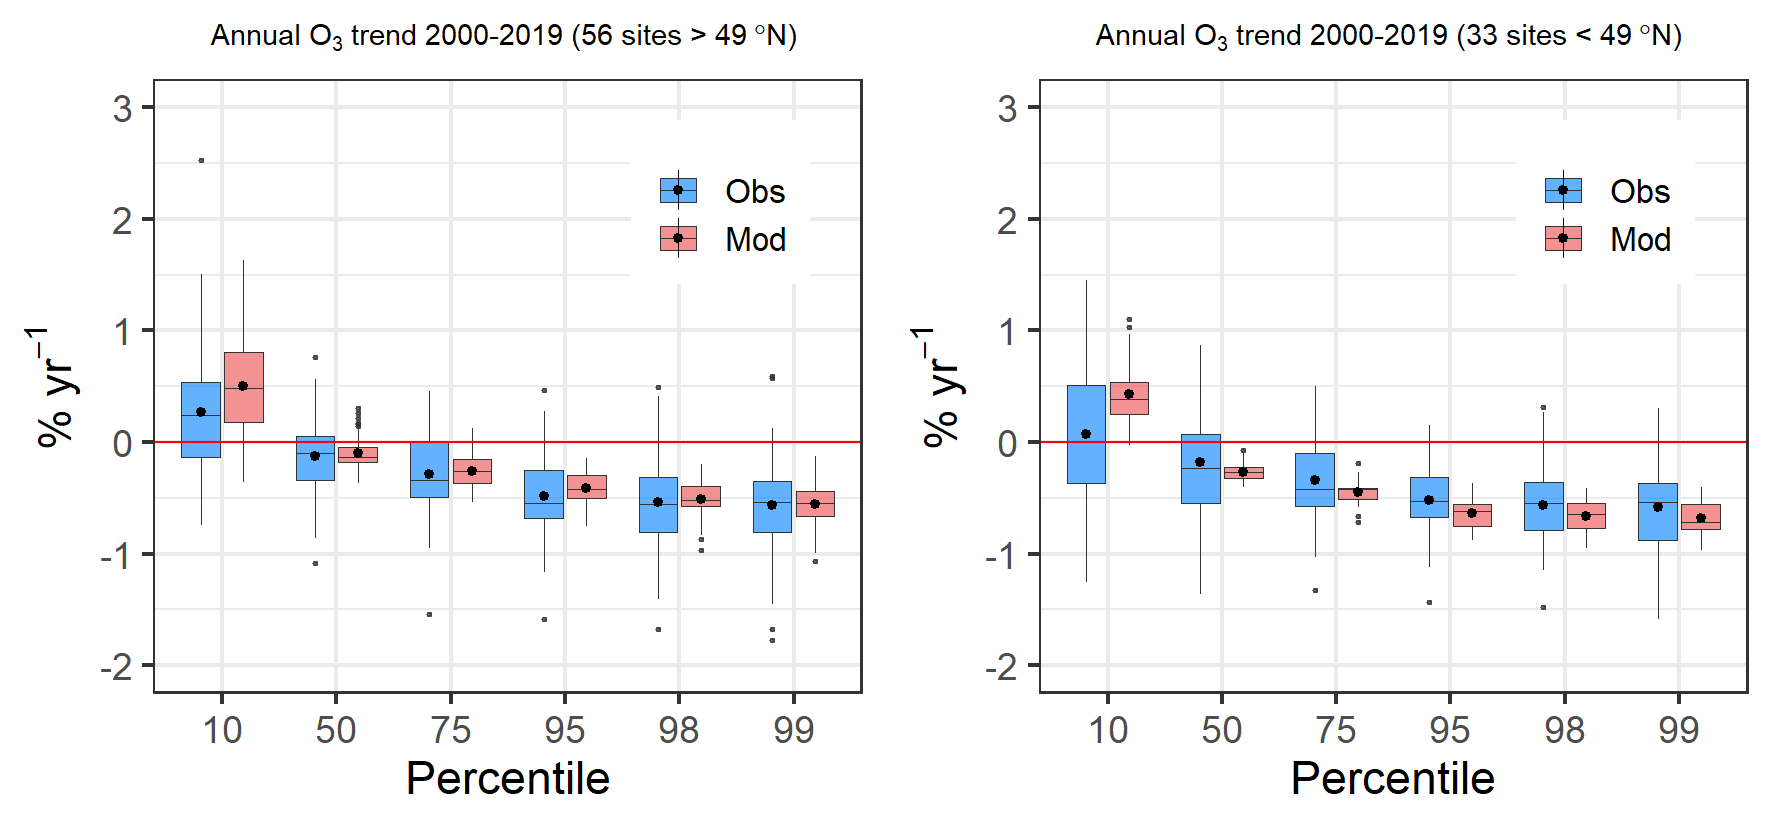
\includegraphics[width=0.74\paperwidth]{FIGS_TRENDS/O3_boxpl.png}
	\caption{\label{fig:O3_boxplot}Boxplot of trends in annual percentiles of daily max O$_3$ from 2000-2019 for EMEP observations and model calculations for stations north (left) and south (right) of 49 \degrees N. The boxes mark the 25 and the 75 percentiles with the median given as a thin line inside. The upper whisker extends from the hinge to the highest value that is within 1.5*IQR of the hinge, where IQR is the inter-quartile range, or distance between the first and third quartiles. The lower whisker extends from the hinge to the lowest value within 1.5*IQR of the hinge. Data beyond the end of the whiskers are outliers and plotted as points. The mean values are shown as black circles. Both significant and non-significant trend values were included. Only sites below 1200 m asl and with at least 15 years of data are included.}
\end{figure}

\begin{figure}[h]
	\centering
	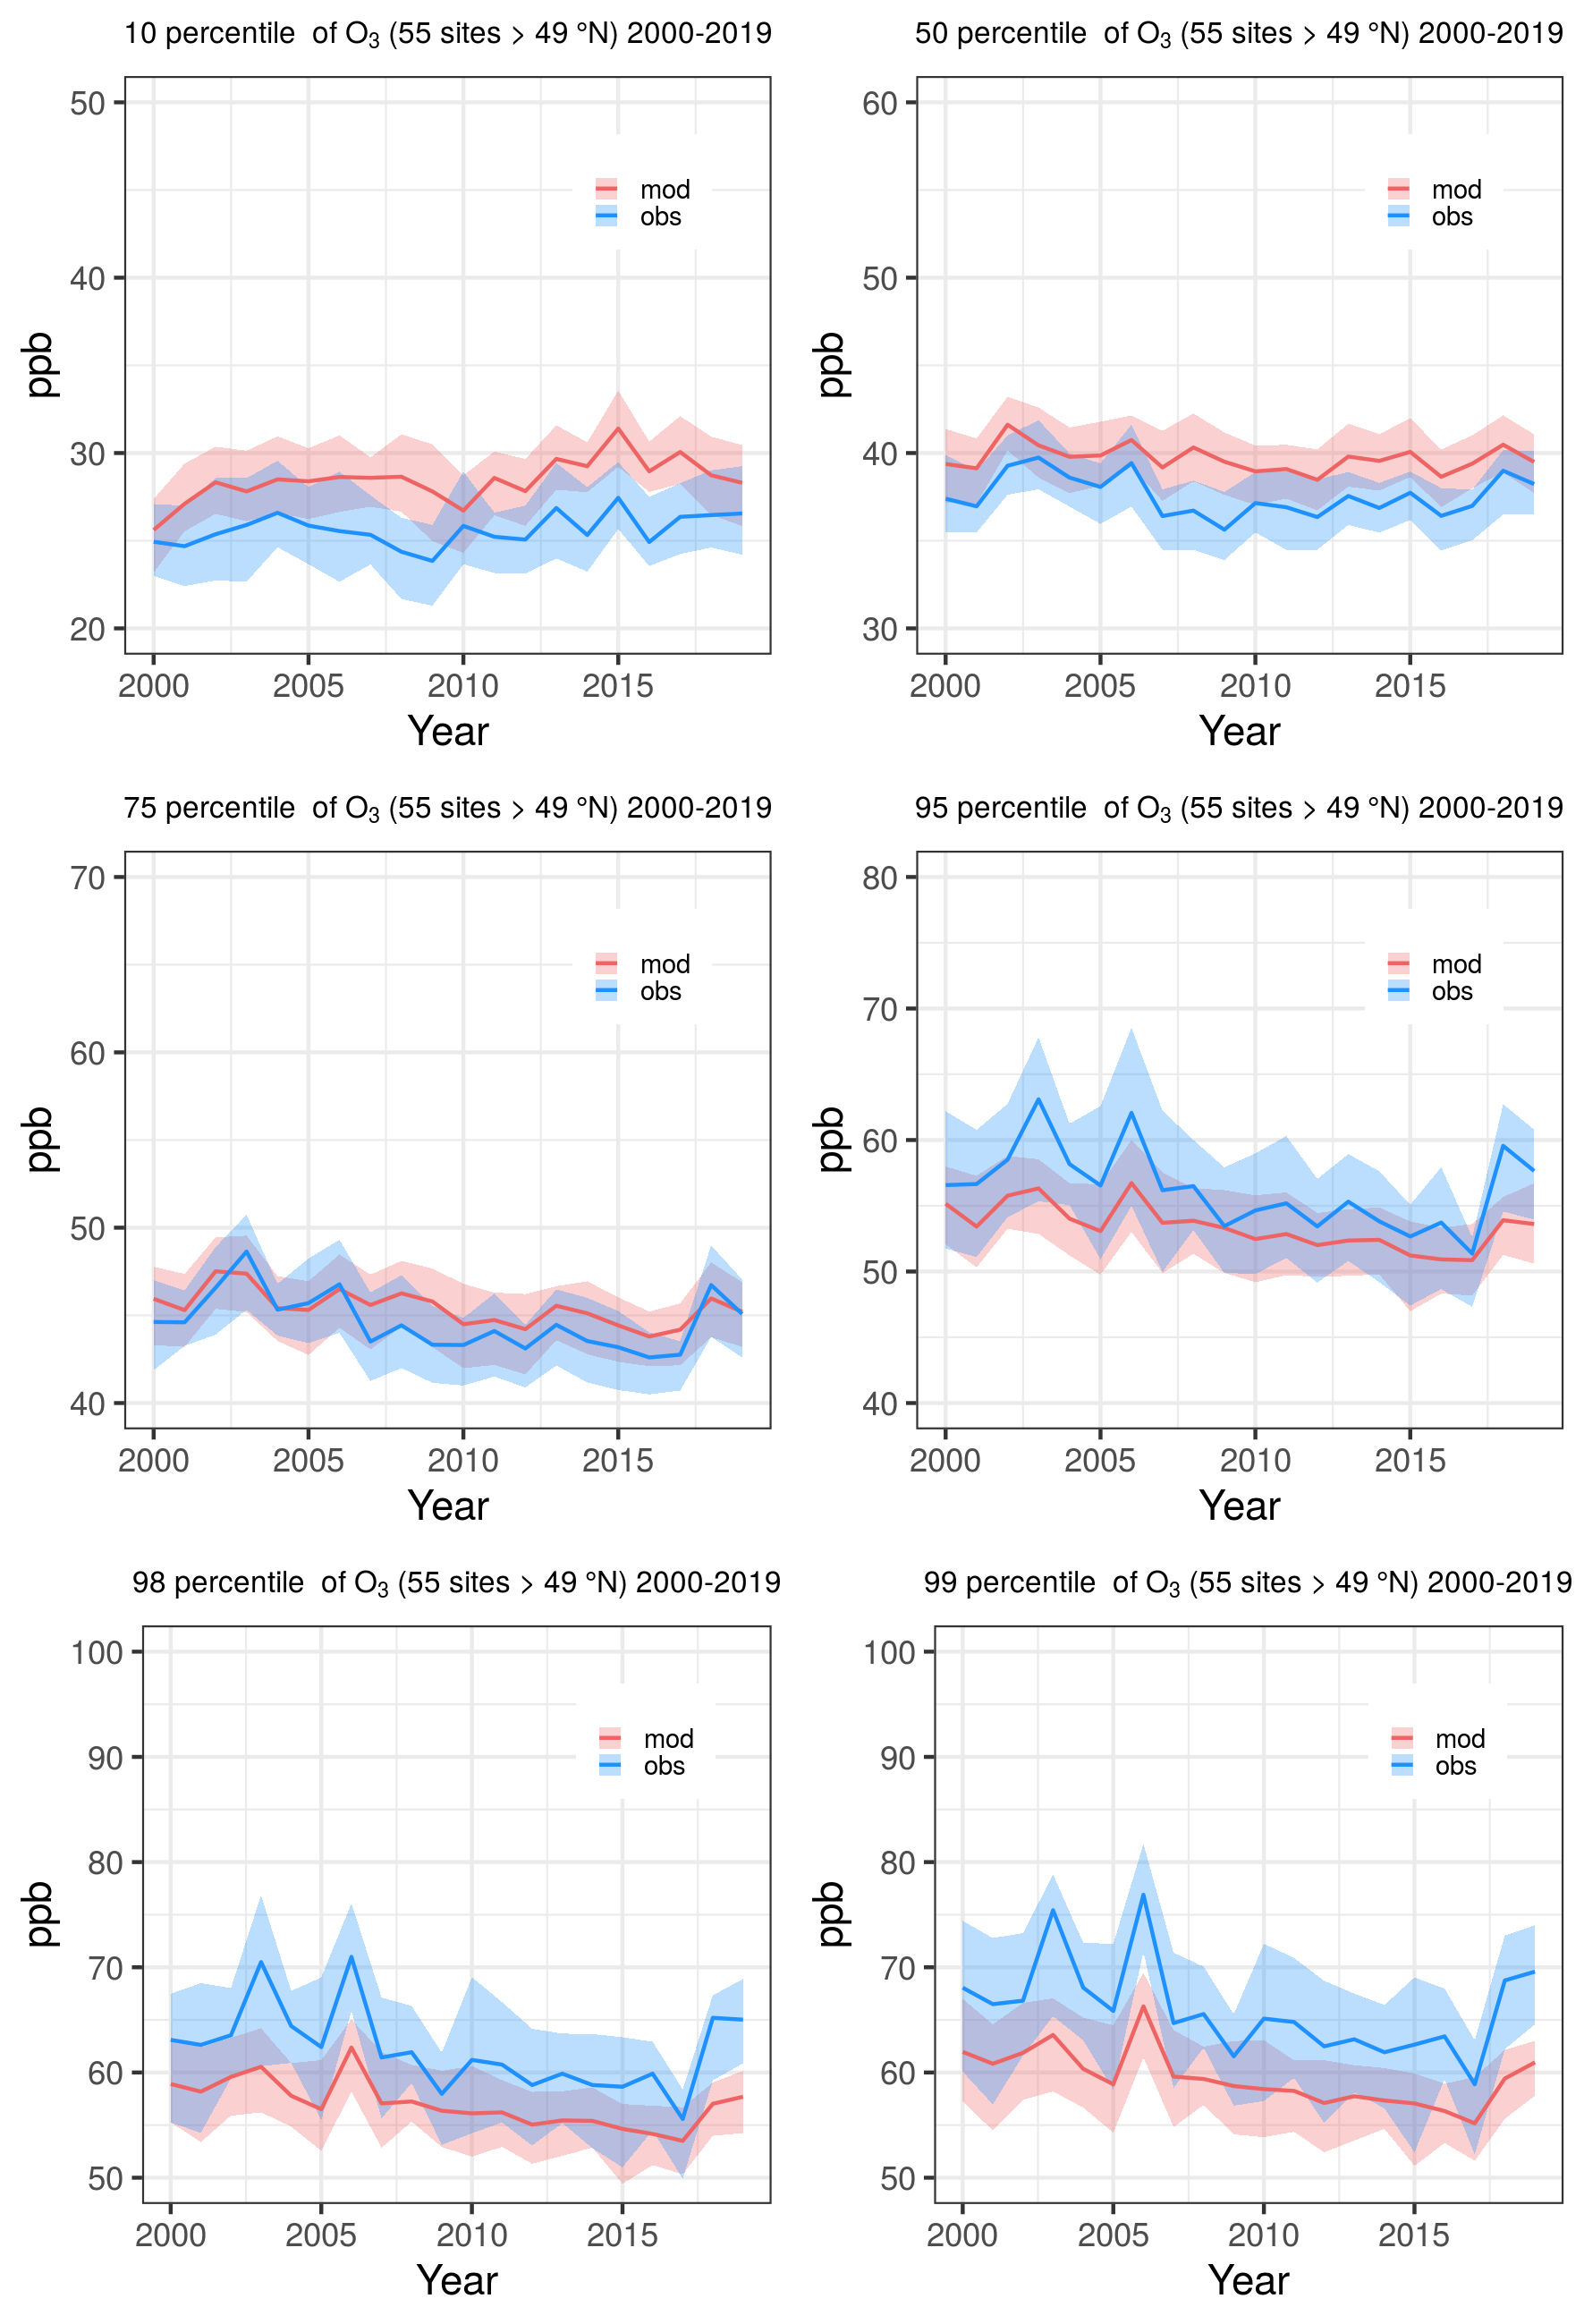
\includegraphics[width=0.74\paperwidth]{FIGS_TRENDS/alltrends_north_49_2000_2019_1200m.png}
	\caption{\label{fig:O3_perctrends_N}Trends in annual percentiles of daily max O$_3$ from 2000-2019 for EMEP observations and model calculations for sites north of 49 \degrees N: The solid line indicates the mean, and the shaded area marks the 25th and 75th percentile. Only sites below 1200 m asl and with at least 15 years of data are included.}
\end{figure}

\begin{figure}[h]
	\centering
	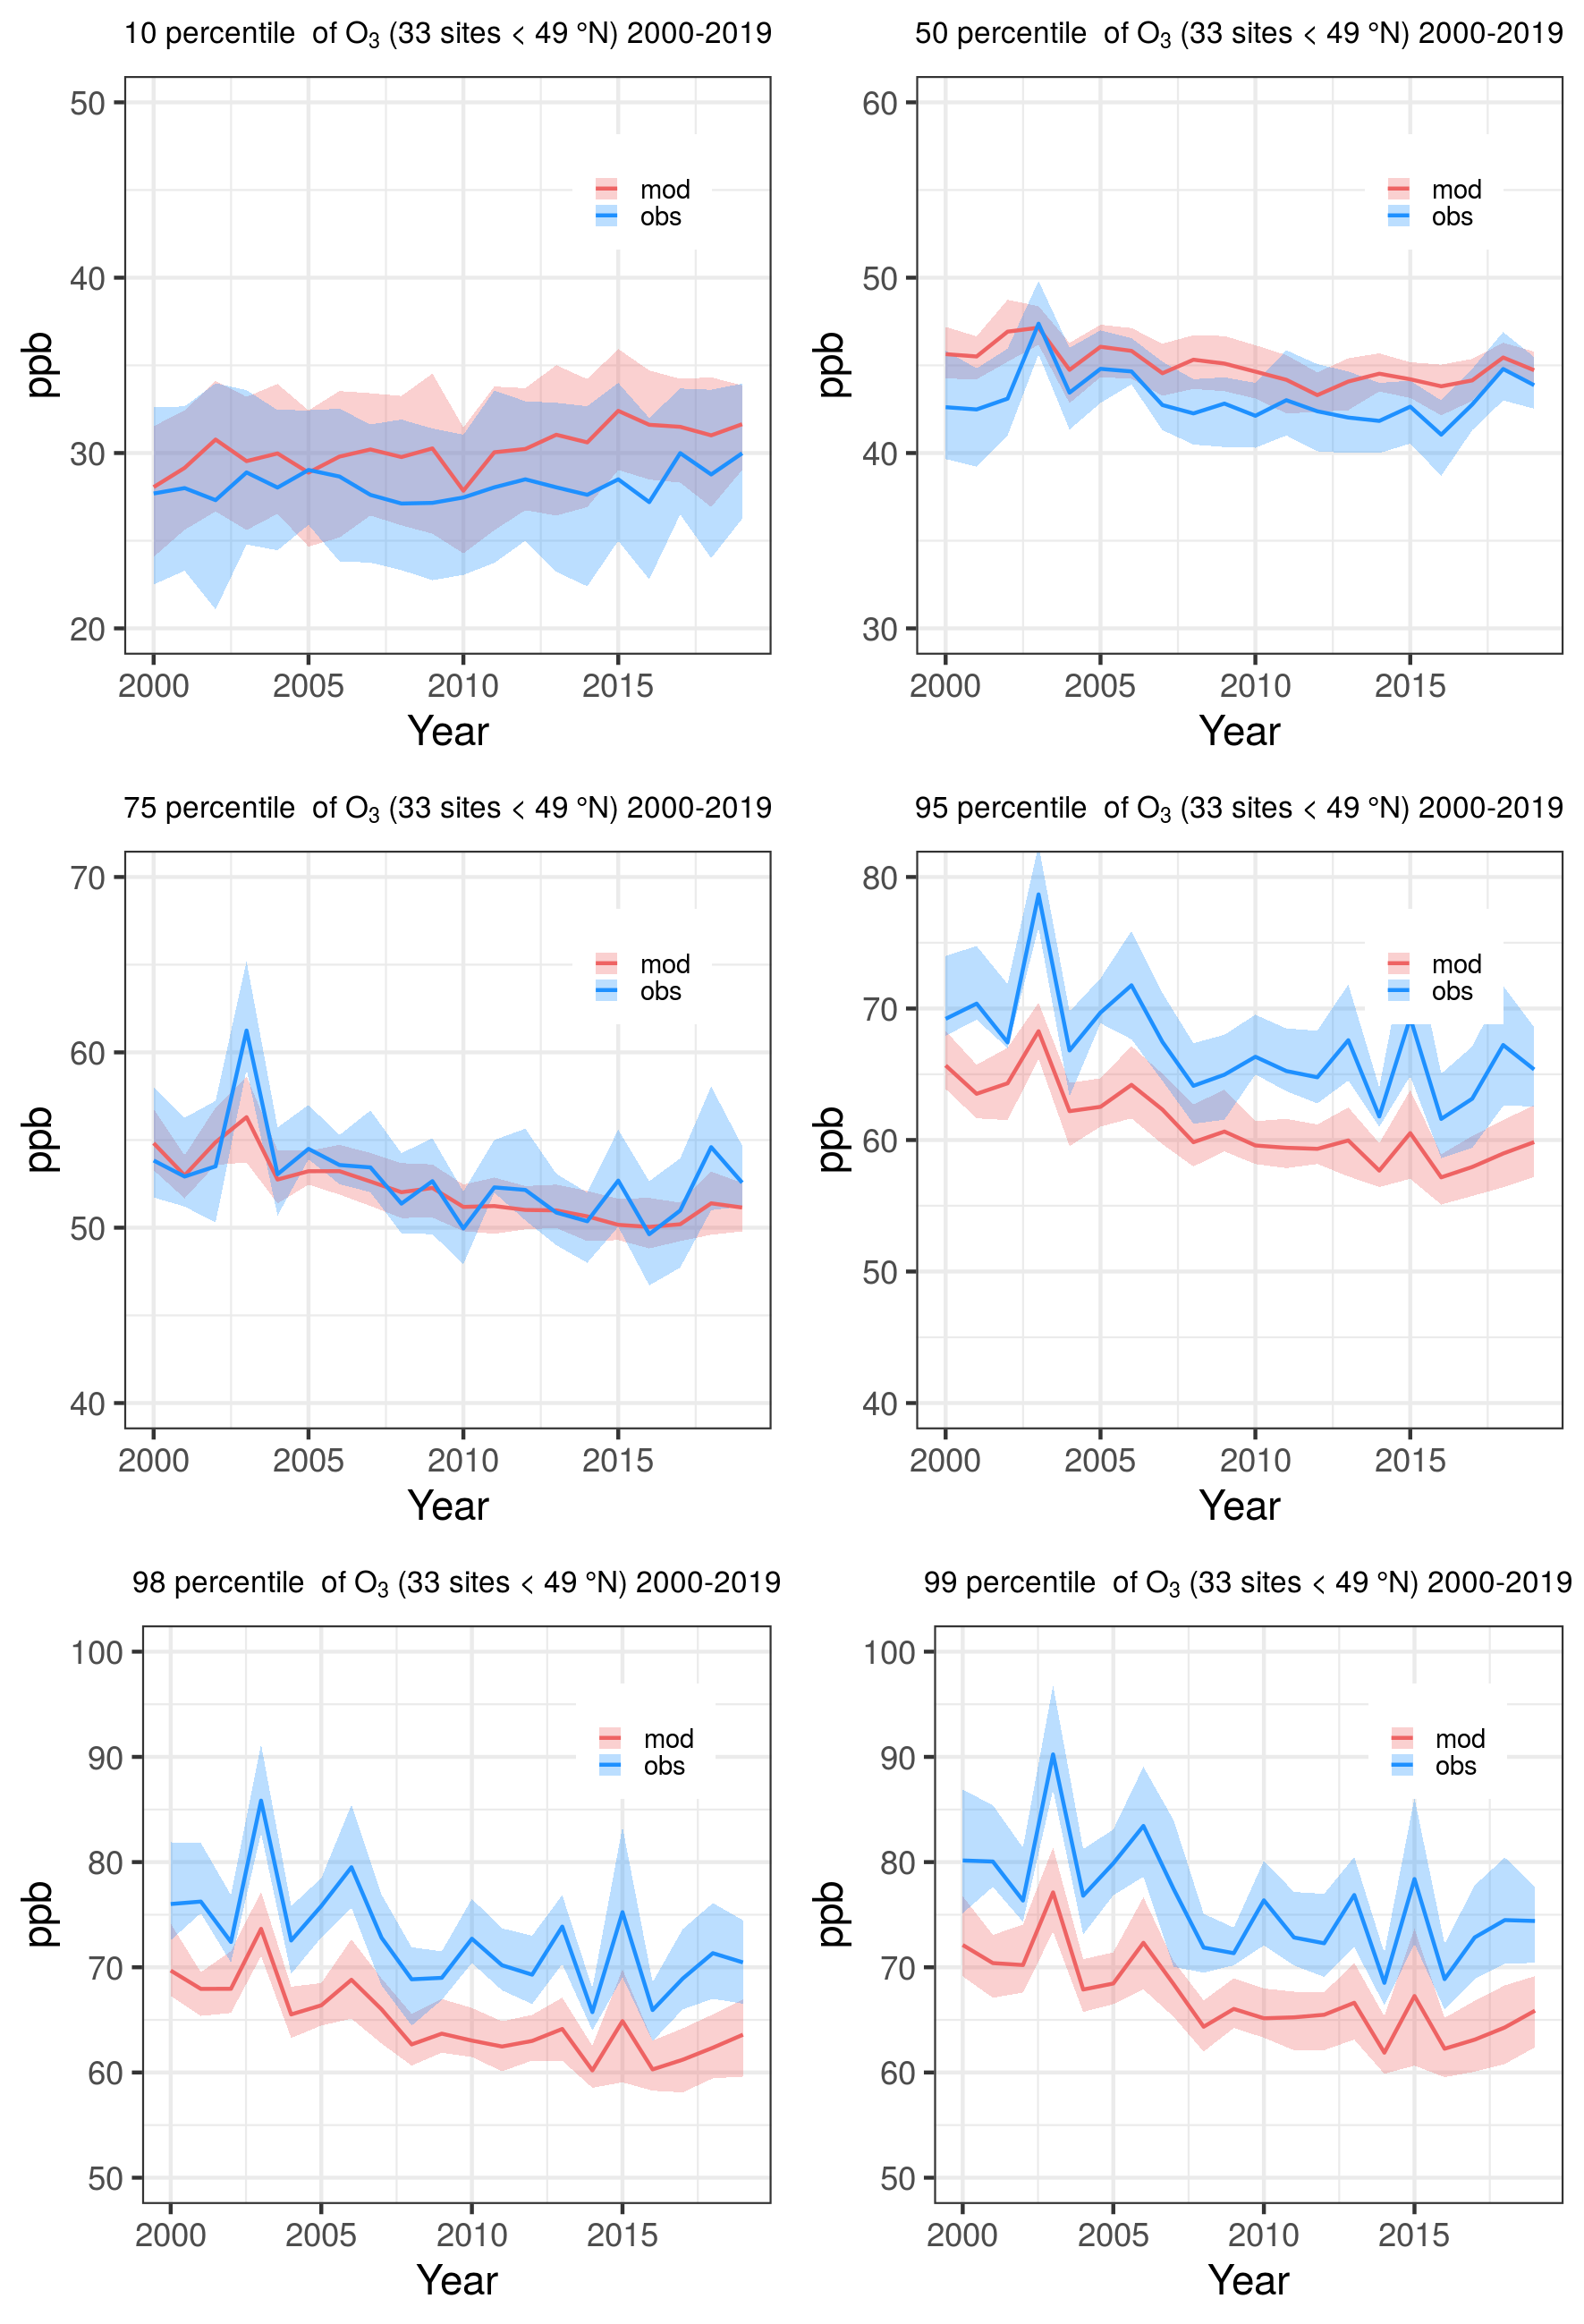
\includegraphics[width=0.74\paperwidth]{FIGS_TRENDS/alltrends_south_49_2000_2019_1200m.png}
	\caption{\label{fig:O3_perctrends_S}Trends in annual percentiles of daily max O$_3$ from 2000-2019 for EMEP observations and model calculations for sites south of 49 \degrees N: The solid line indicates the mean, and the shaded area marks the 25th and 75th percentile. Only sites below 1200 m asl and with at least 15 years of data are included.}
\end{figure}

\begin{figure}[h]
	\centering
	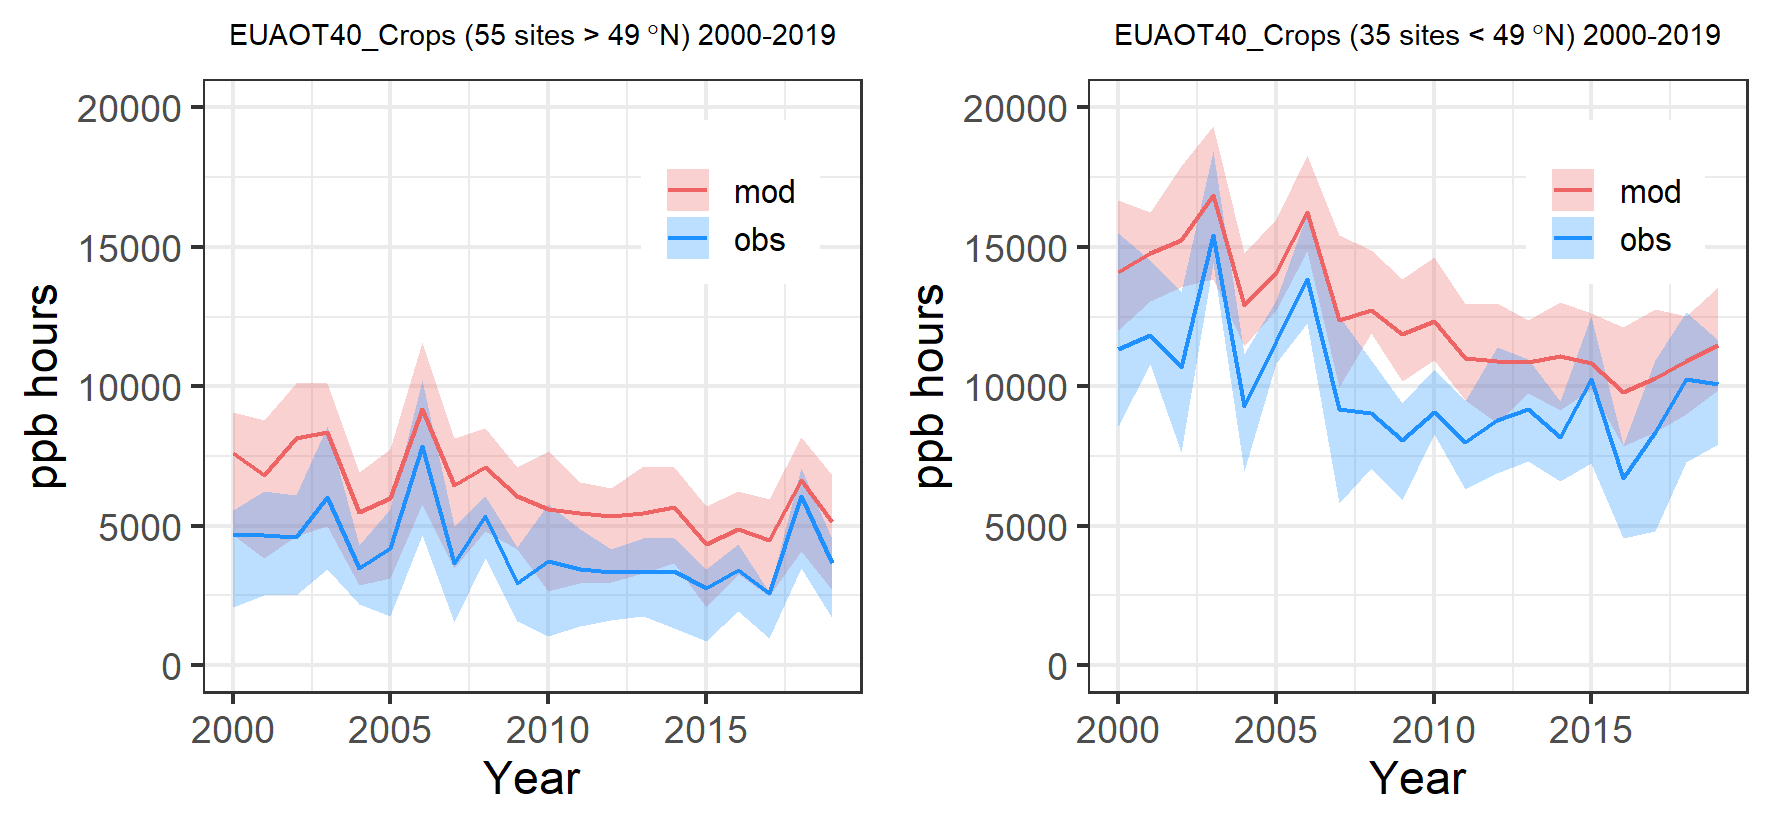
\includegraphics[width=0.74\paperwidth]{FIGS_TRENDS/EUAOT40_Crops_2000_2019_1200m.png}
	\caption{\label{fig:O3_aot40croptrends} Trends in 3-months AOT40 (May-July) for crops from 2000-2019 for EMEP observations and model calculations for sites north (left) and south (right) of 49 \degrees N: The solid line indicates the mean, and the shaded area marks the 25th and 75th percentile. Only sites below 1200 m asl and with at least 15 years of data are included.}
\end{figure}

\begin{figure}[h]
	\centering
	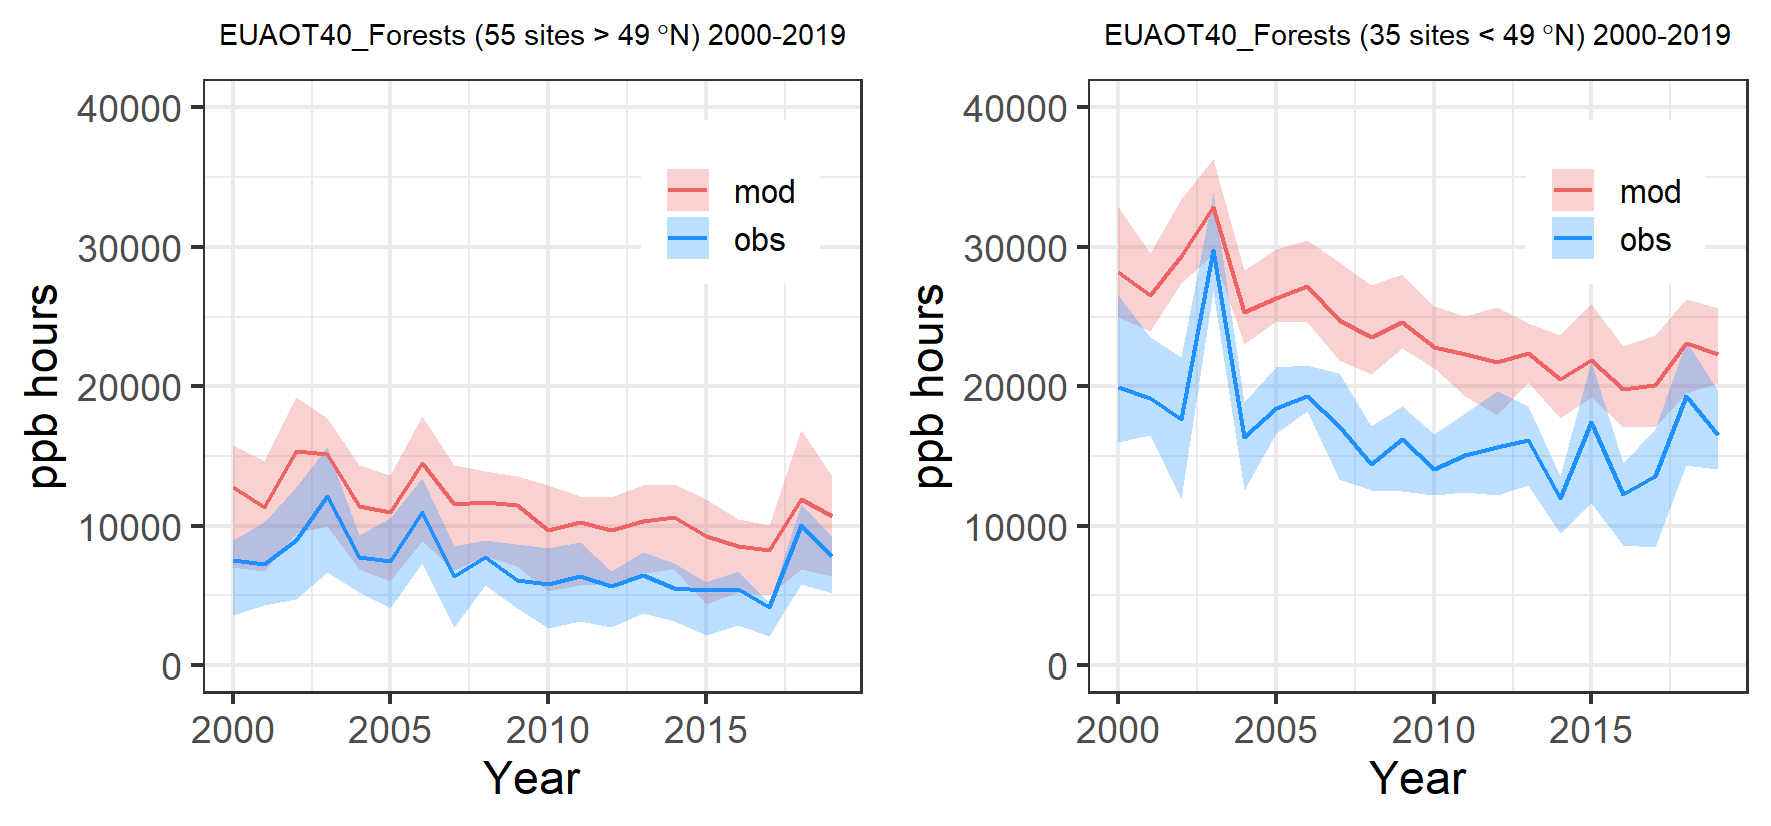
\includegraphics[width=0.74\paperwidth]{FIGS_TRENDS/EUAOT40_Forests_2000_2019_1200m.png}
	\caption{\label{fig:O3_aot40foresttrends}Trends in 6-months AOT40 (Apr-Sep) for forests from 2000-2019 for EMEP observations and model calculations for sites north (left) and south (right) of 49 \degrees N: The solid line indicates the mean, and the shaded area marks the 25th and 75th percentile. Only sites below 1200 m asl and with at least 15 years of data are included.}
\end{figure}

\begin{figure}[h]
	\centering
	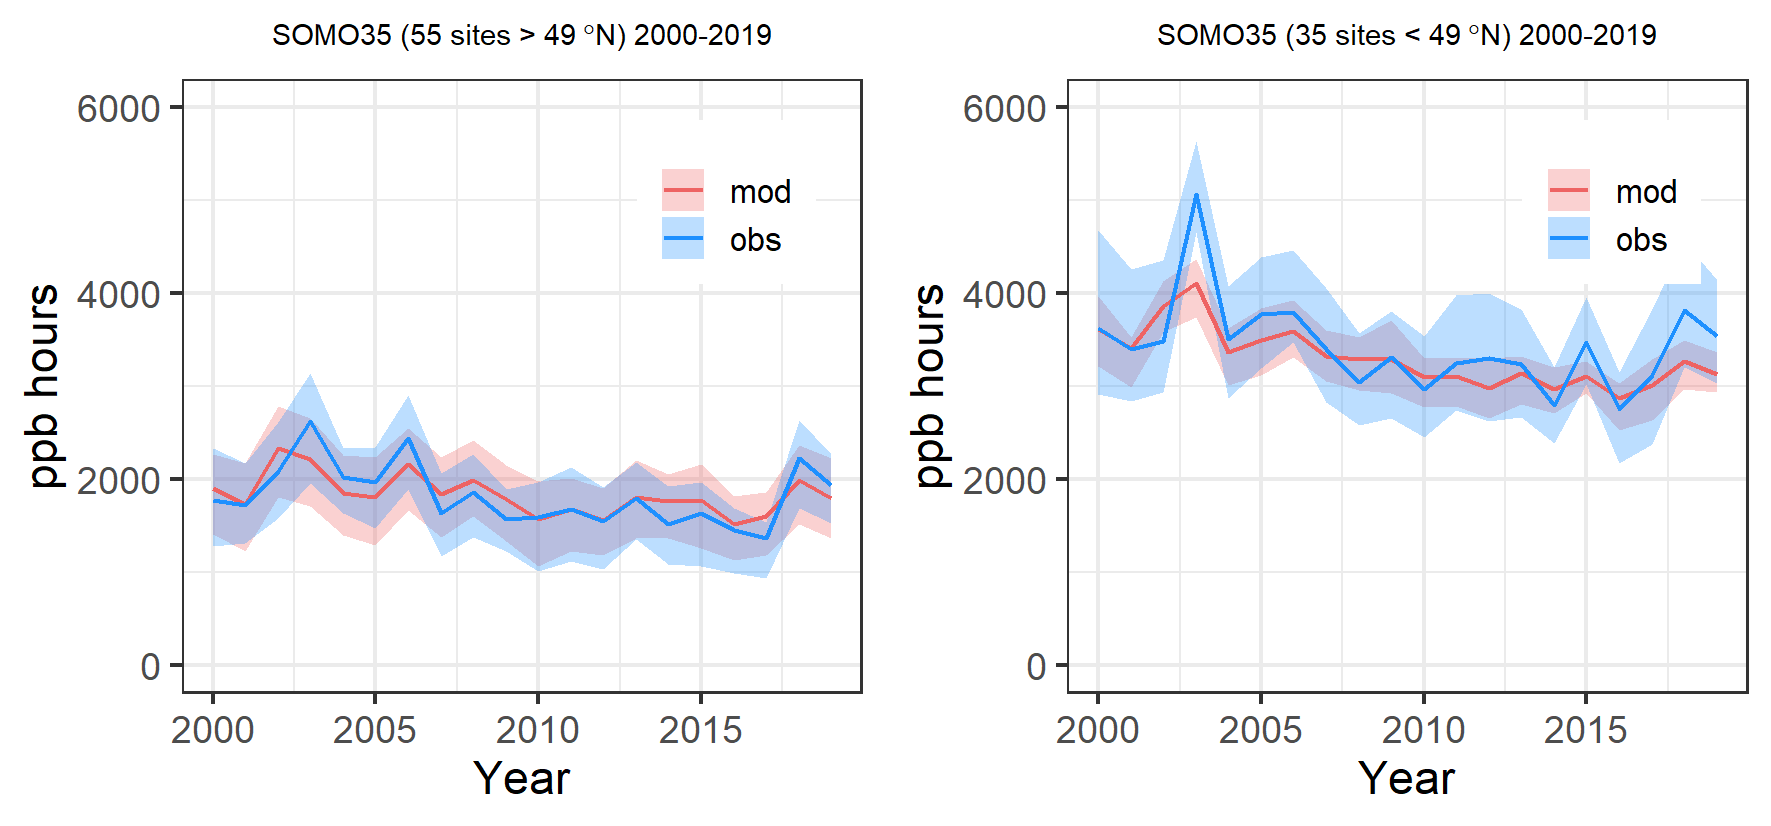
\includegraphics[width=0.74\paperwidth]{FIGS_TRENDS/SOMO35_2000_2019_1200m.png}
	\caption{\label{fig:O3_somo35trends}Trends in SOMO35 from 2000-2019 for EMEP observations and model calculations for sites north (left) and south (right) of 49 \degrees N: The solid line indicates the mean, and the shaded area marks the 25th and 75th percentile. Only sites below 1200 m asl and with at least 15 years of data are included.}
\end{figure}


%%%%%%%%%%%%%%%%%%%%%%%%%%%%%%%%%%%%%%%%%%%%%%%%%%%%%%%%%%%%%%%%%%%%%%%%%%%%

\clearpage
\section{Trends in Elemental and Organic Carbon}
\label{sec:trendsECOC}
\subsection{Elemental Carbon, EC}
\label{ss:trendsEC}

Table~\ref{tab:KEX1} presents the absolute and relative changes over 2010-2019 from 15 EMEP sites, as annual values, and with confidence intervals, and from both observed and modelled values. The spatial variation of these trends for summer and winter can be seen as `arrow' plots in Fig.~\ref{fig:ECarrows}, and Fig.\ref{fig:ECtrends} shows again the annual trends, but superimposed upon the field of modelled EC.
Fig.~\ref{fig:KEX1} illustrates the statistics of the reductions in EC over the period 2010-2019, and for different seasons. 

%
Considering first the observed trends in elemental carbon (EC) for 2010--2019, a  reduction (-4.5$\pm$1.5~\%/yr, Tab.~\ref{tab:KEX1}) 
 was
calculated for the 15 sites assessed, which is
quite comparable to the reduction (-5.0$\pm$0.9~\%/yr)
calculated for the eleven sites where the reduction was statistically
significant. The reduction was rather similar considering these eleven
sites, ranging from -4.2~\%/yr to -5.8~\%/yr for ten out of eleven
sites. %, thus we see no apparent spatial pattern in the reductions
The largest reduction was seen amongst the sites with the
highest EC levels, i.e., at Iskrba (-7~\%/yr) in Slovenia and at Ispra
(-5.8~\%/yr) in the Po Valley region in Northern Italy (Fig.~\ref{fig:ECtrends}). Notably, these
were the only sites where a statistically significant reduction was
observed for all seasons, being most pronounced in summer, although
by a small margin. When considering all sites, the reduction was most
pronounced in summer and fall (Tab.~\ref{tab:KEX1},Fig.~\ref{fig:KEX1}), but the general picture is
that there is a minor seasonal variability in the reduction of EC. It can be noted though that
there are more sites with significant trends (p-values $<$ 0.05)  in summer than winter (Fig.\ref{fig:ECarrows}).

Fig.~\ref{fig:KEX1} illustrates the statistics of the reductions in EC  n both observed and model results over the period 2010-2019, and for different seasons. For EC the model is seen to capture the year to year changes very well over the ten years, and captures well the relative changes which are ca. -4~\%/yr in all seasons. Larger differences are seen in the absolute changes (which may reflect the difficulties with the EC emissions mentioned in Sect.~\ref{ss:IssuesECOC}).
These points about model-measurement comparison for EC are discussed further in Sect.~\ref{ss:DiscECOC}.

\begin{table}
 \caption{Absolute change (\ugC/yr) and relative change (\%/yr) and
  corresponding confidence intervals in observed and modelled annual
  and seasonal aggregated EC concentrations at 15 sites across Europe
  for 2010--2019. The number of sites with a significant outcome is
  provided. \label{tab:KEX1}}
% \begin{tabular}{lrrrrlrlrlrl}
%\begin{center}
\scalebox{0.65}{%
\begin{tabular}{llcc|cccc|cccc}
\toprule
%\hline
               \multicolumn{4}{c}{Number of sites} & \multicolumn{4}{c}{Absolute change (\ug $yr^{-1})$} & \multicolumn{4}{c}{Relative change (\% $yr^{-1}$)} \\
 Season &           Total & Sign. & Sign. &                   obs. &          Conf.interval &  Mod. &          Conf.interval &                     Obs. &         Conf.interval &  Mod. &        Conf.interval \\
       &                  & (Obs.)    & (Mod.)     &   &  &  & & & & & \\
\midrule
%\hline
All    &              15 &         11 &          12 &                  -0.019 &  (-0.031, -0.008) & -0.014 &  (-0.021, -0.007) &                    -4.49 &  (-5.25, -3.73) & -3.81 &  (-4.59, -3.03) \\
Winter &              15 &          6 &           4 &                  -0.029 &  (-0.053, -0.006) & -0.019 &  (-0.032, -0.006) &                    -4.27 &  (-5.49, -3.06) & -3.10 &  (-4.21, -1.98) \\
Spring &              15 &          5 &           8 &                  -0.012 &  (-0.018, -0.006) & -0.013 &  (-0.018, -0.009) &                    -3.88 &  (-4.67, -3.09) & -3.86 &   (-4.92, -2.8) \\
Summer &              15 &          8 &          10 &                  -0.011 &  (-0.015, -0.007) & -0.008 &  (-0.013, -0.004) &                    -4.73 &  (-5.71, -3.74) & -3.71 &  (-4.59,  -2.82) \\
Autumn &              15 &          8 &          11 &                  -0.023 &   (-0.036, -0.01) & -0.018 &  (-0.027, -0.009) &                    -4.96 &   (-6.03, -3.9) & -4.25 &  (-5.15,  -3.35) \\
\bottomrule
\end{tabular}
} % end scalebox
\end{table}

%%%%%%%%%%%%%%%%%%%%%%%%%%%%%%%%%%%%%%%%%%%%%%%%%
% trim L L R U 
\begin{figure}
\includegraphics*[height=6cm,trim=3cm 0 0 0]{FIGS_TRENDS/Plot_ec_rel_summer_Model.png}%
\includegraphics*[height=6cm,trim=3cm 0 6.5cm 0]{FIGS_TRENDS/Plot_ec_rel_summer_Observations.png}
\\
\includegraphics*[height=6cm,trim=3cm 0 0 0]{FIGS_TRENDS/Plot_ec_rel_winter_Model.png}%
\includegraphics*[height=6cm,trim=3cm 0 6.5cm 0]{FIGS_TRENDS/Plot_ec_rel_winter_Observations.png}
\caption{Relative trends for EC in \pmfine over the period of 2010-2019, from both model (left) and observations (right), and for summer (top) and winter (bottom). The magnitude of the trends is indicated by the angle made (see key), which also indicates the trend values associated with 45\degrees and 90\degrees angles. The colour indicates the p-values associated with the trends. (The style of these plots is based upon those used in the ROAR project, e.g.\citealt{MillsTOAR:2018}.) 
  \label{fig:ECarrows}}
\end{figure}
%%%%%%%%%%%%%%%%%%%%%%%%%%%%%%%%%%%%%%%%%%%%%%%%%
%%%%%%%%%%%%%%%%%%%%%%%%%%%%%%%%%%%%%%%%%%%%%%%%%%%%%%
\begin{figure}  %DS[H]
  \centering{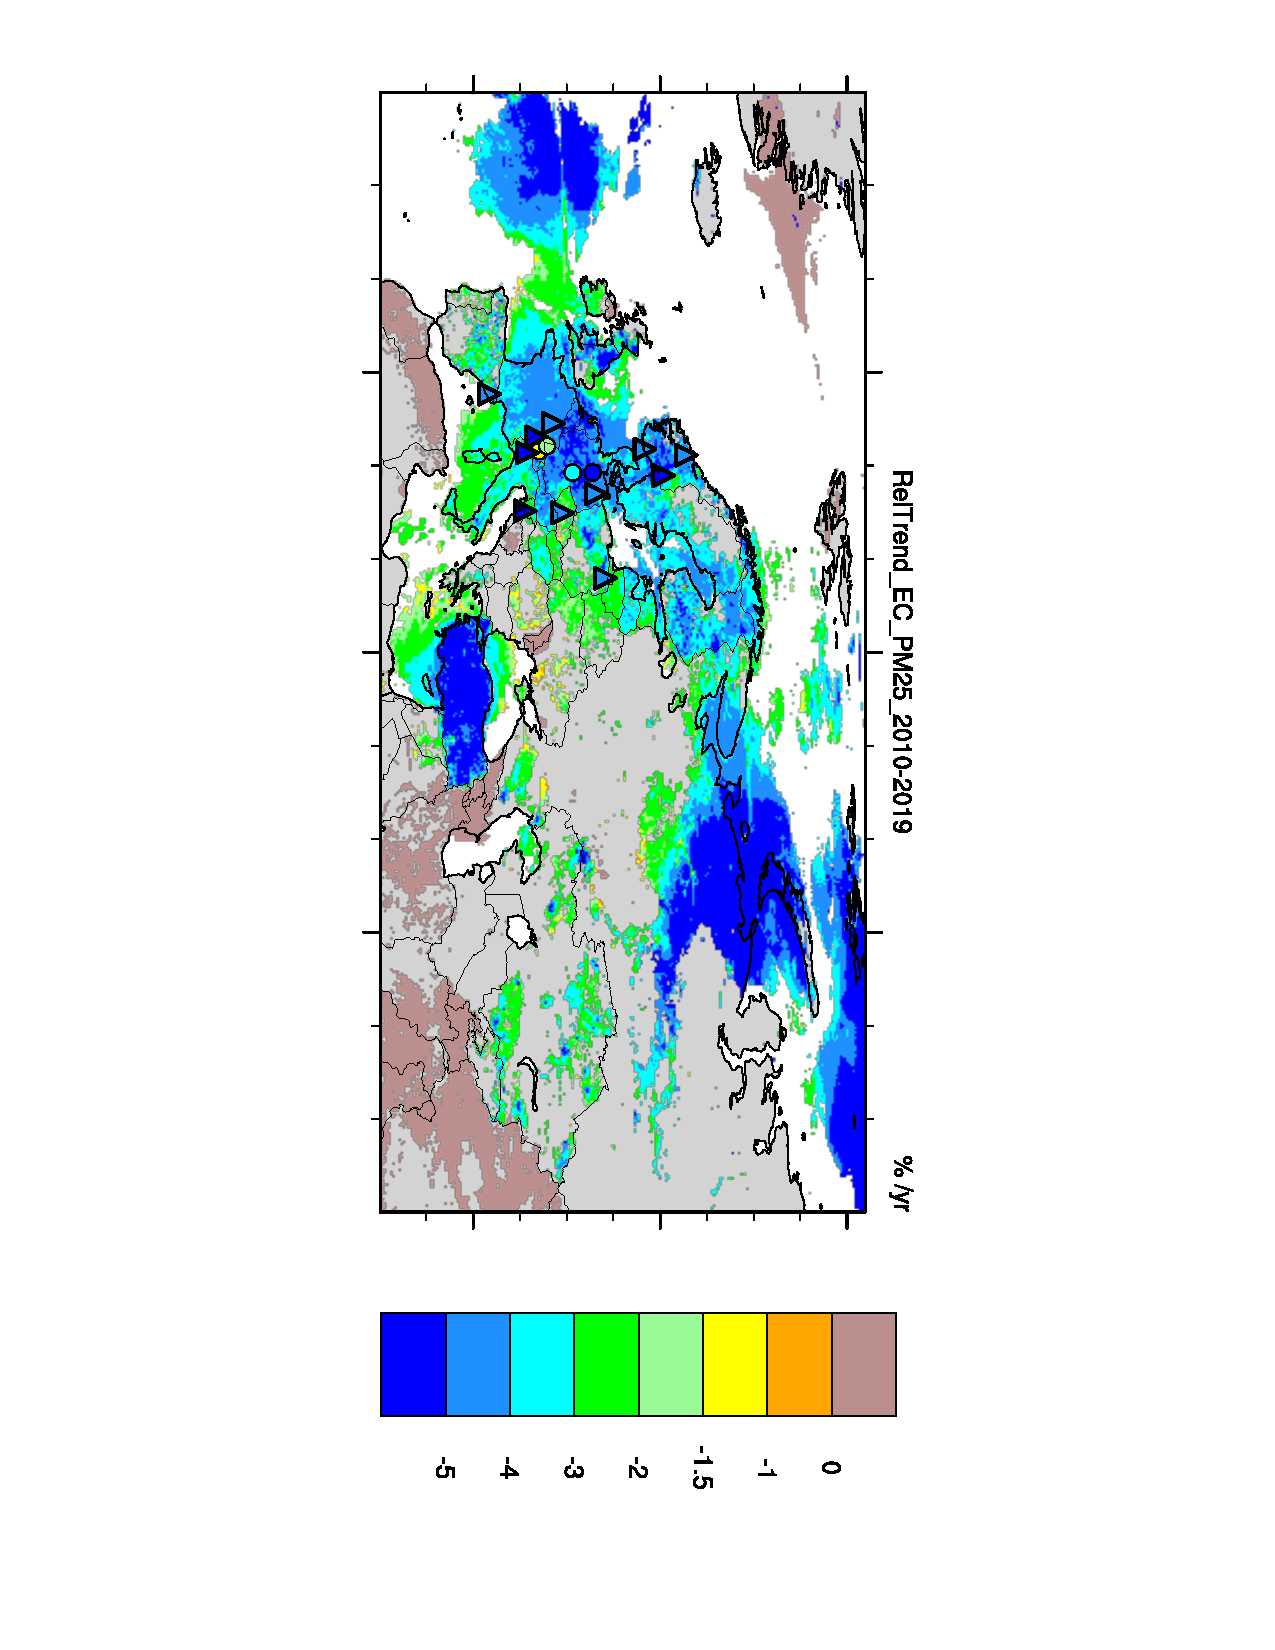
\includegraphics[clip=,angle=90,height=6.1cm,viewport=175 67 448 754]{FIGS_TRENDS/RelTrend_EC_PM25_2010-2019_Perc.pdf}}\\
%  \vspace{0.5cm}
%  \centering{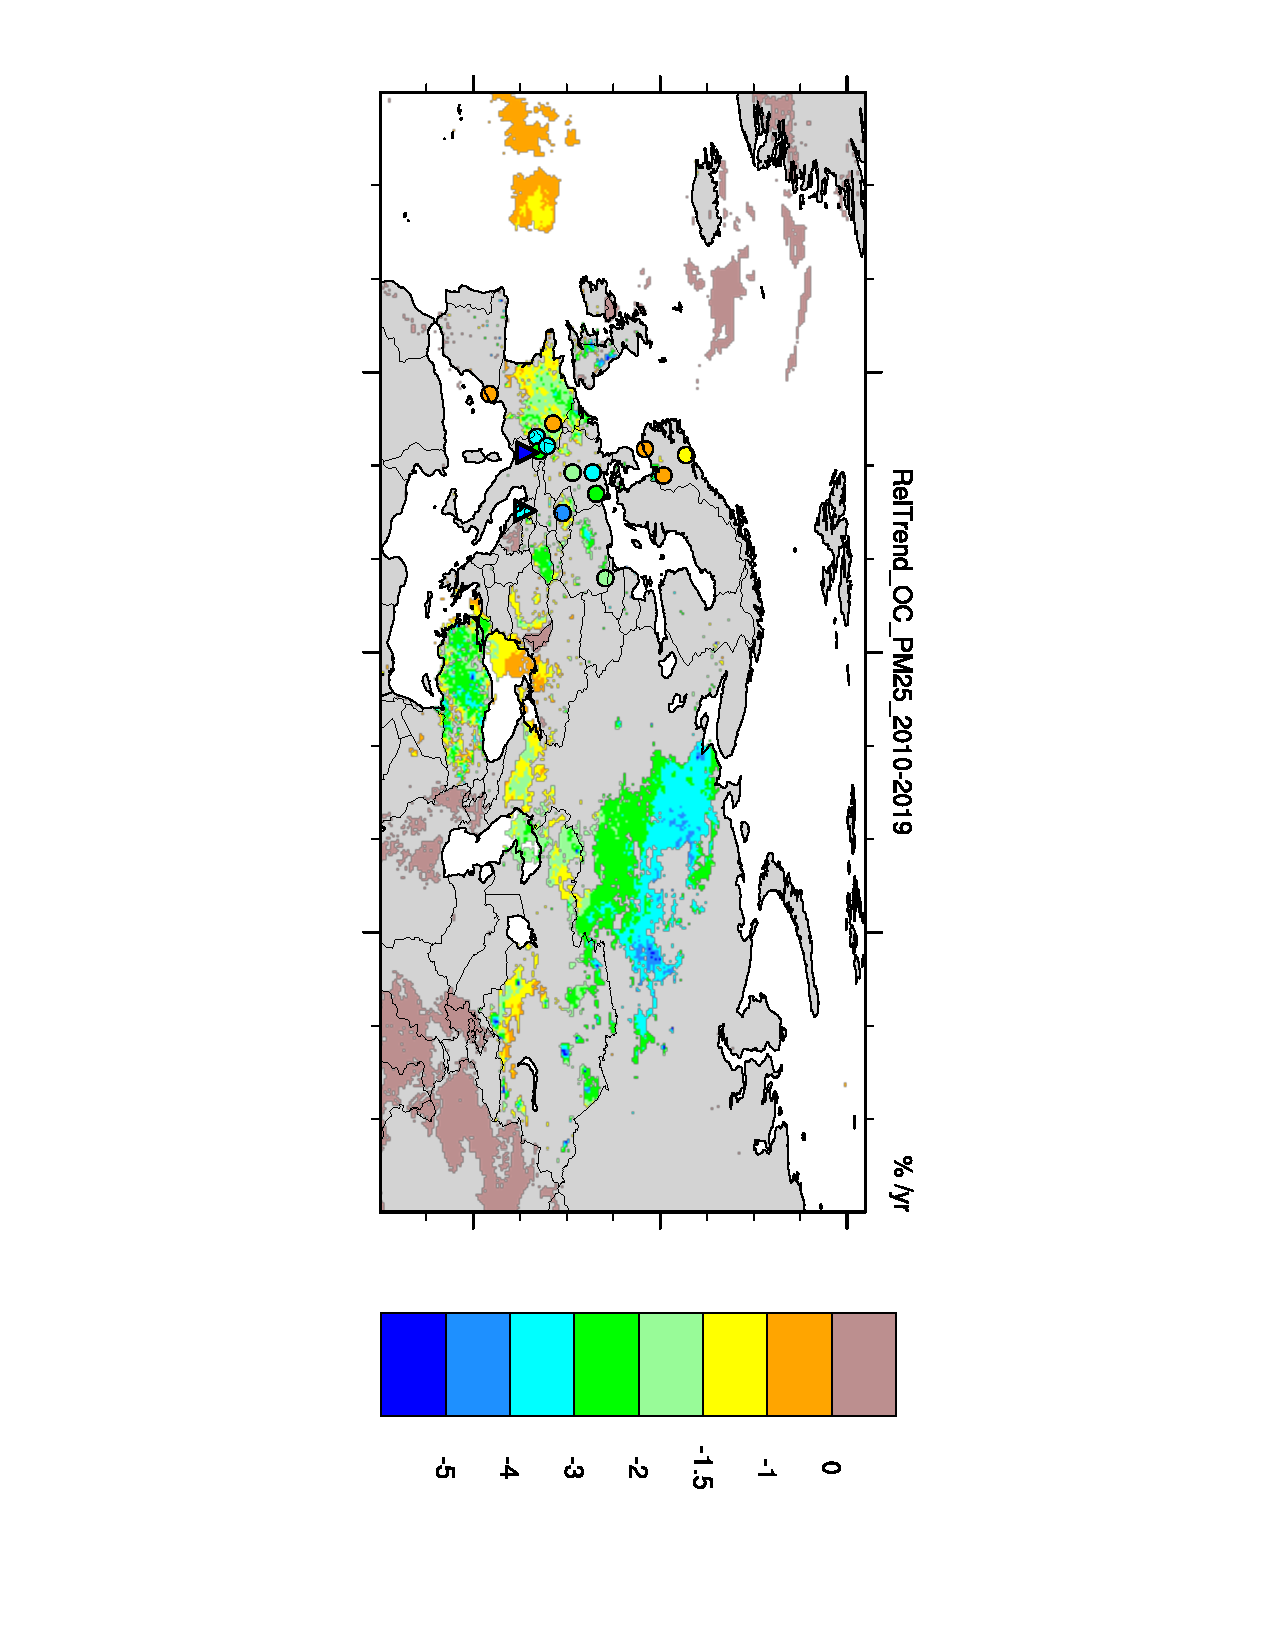
\includegraphics[clip=,angle=90,height=6.1cm,viewport=175 67 448 754]{FIGS_TRENDS/RelTrend_OC_PM25_2010-2019_Perc.pdf}}
\caption{Relative trends for EC in \pmfine over the period of 2010-2019: EMEP modelled -- coloured contours (grey/white means non-significant trends) and observed - coloured triangles (significant) and circles (non-significant).}
\label{fig:ECtrends}
\end{figure}
%%%%%%%%%%%%%%%%%%%%%%%%%%%%%%%%%%%%%%%%%%%%%%%%%


\begin{figure}[t]
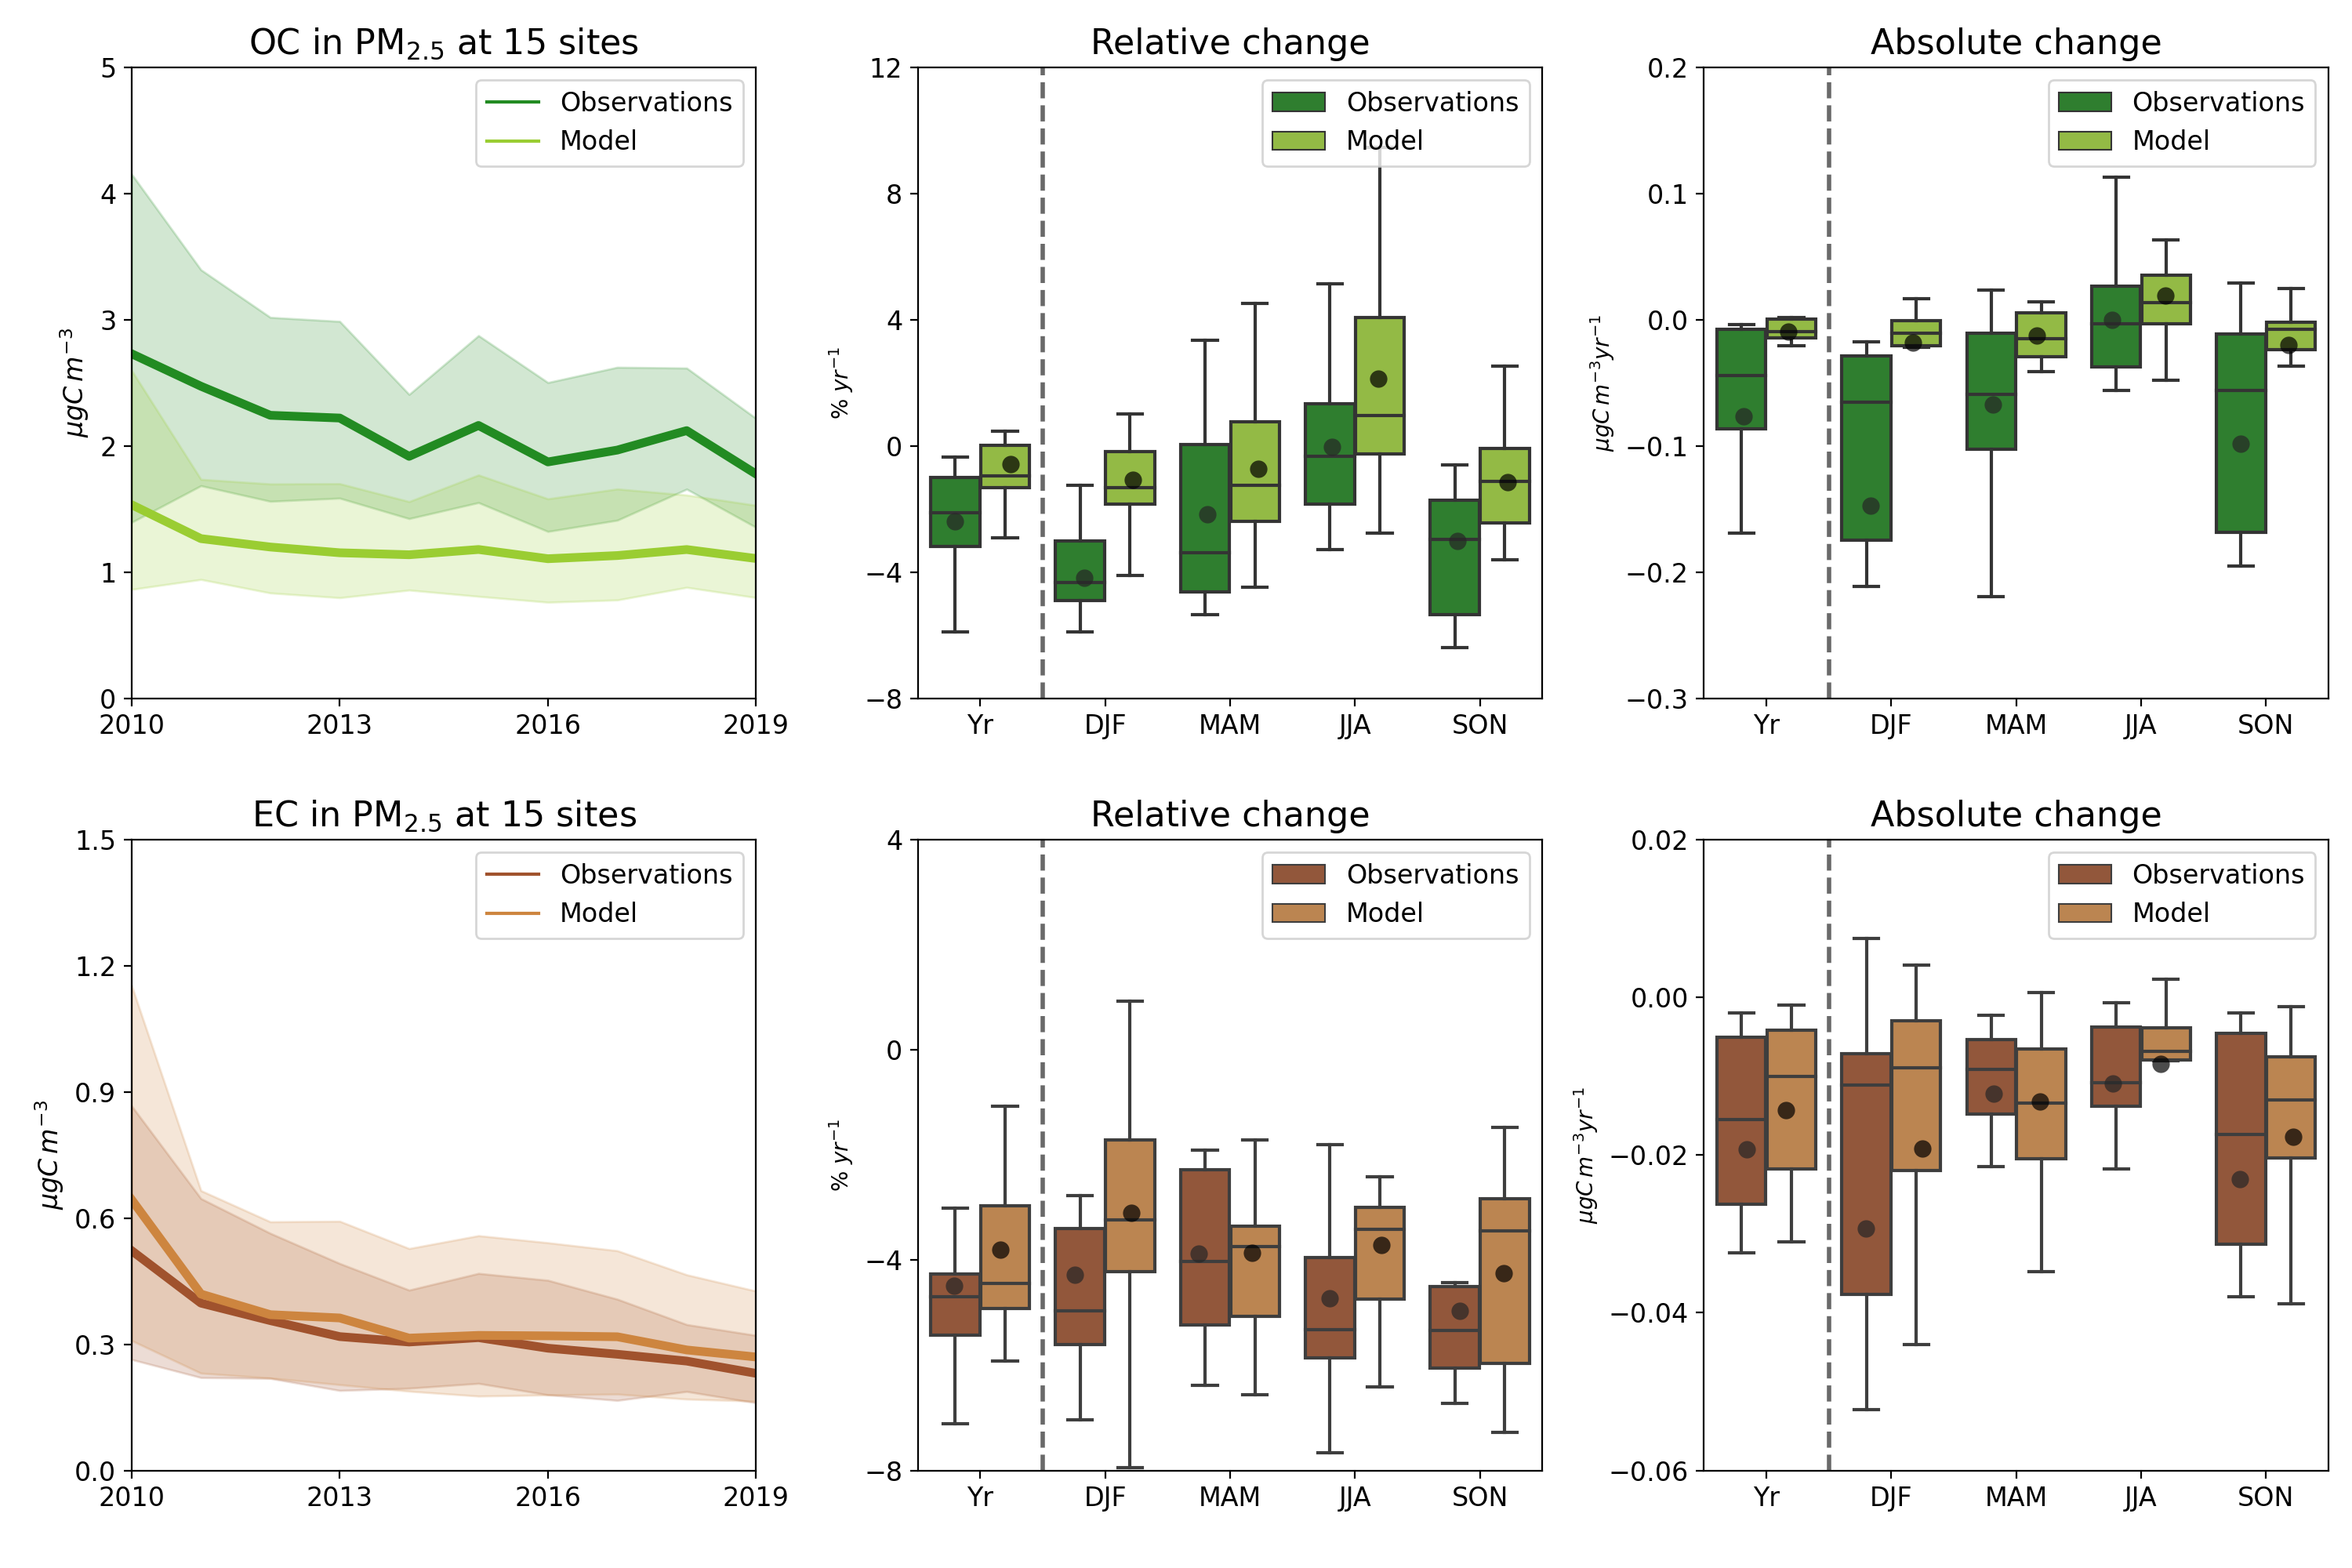
\includegraphics[width=16cm]{FIGS_TRENDS/ECOC_trends.png}
\caption{Observed and modelled concentrations and trends of EC and OC at 15 EMEP
  site across Europe for 2010--2019, showing the concentrations
  (left panels) of OC (upper) and EC (lower), aggregated annual and
  seasonal relative changes (mid panels) for OC (upper) and EC (lower),
  and aggregated annual and seasonal absolute changes (right panels)
  for OC (upper) and EC (lower). The solid line in the left panel shows
  the average annual mean for all sites and the shaded area the 95\%
  confidence interval. The box plots in the mid and right panels show
  the 25th and 75th percentiles (boxes), the median (horizontal lines),
  whereas the whiskers represent the interquartile ranges $\times$
  1.5 and the squares the outliers. Black markers within the box are
  the means.\label{fig:KEX1}
}
\end{figure}







\subsection{Organic Carbon, OC}
\label{ss:trendsOC}
 
 Table~\ref{tab:KEX2} presents the absolute and relative changes in OC over 2010-2019 from 15 EMEP sites, as annual values and with confidence intervals, and from both observed and modelled values. The spatial variation of these trends for summer and winter can be seen as `arrow' plots in Fig.~\ref{fig:OCarrows}, and Fig.\ref{fig:OCtrends} shows again the annual trends, but superimposed upon the modelled field of modelled OC.
Fig.~\ref{fig:KEX1} illustrates the statistics of the reductions in OC  over the period 2010-2019, and for different seasons. 
 %
A 2.4$\pm$1.6~\%/yr reduction
  in organic carbon (OC) for 2010--2019
was calculated for the 15 sites assessed (Tab.~\ref{tab:KEX2}), but the
downward trend was statistically significant only for Iskrba (Slovenia)
and Ispra (Italy), which are amongst the sites with the highest OC
loading. At these two sites, the reduction was noticeably higher 
(-3.1~\%/yr at Iskrba, -5.9~\%/yr at Ispra) than for the mean of all sites. The
reduction in OC appears somewhat lower at the westernmost and northernmost
sites (Fig.\ref{fig:OCtrends}). 


% From KE .docx. Assume 
%\begin{figure}
%\caption{Map showing relative change (\%/yr) in observed and modelled OC (left
%  panel) and EC (right panel) at 15 EMEP sites across Europe. \label{fig:KEX2}}
%\end{figure}

There was a pronounced seasonal variability in the reduction observed for
OC (Tab.~\ref{tab:KEX2}, Figs.~\ref{fig:KEX1},\ref{fig:OCarrows}). In winter, the
 reduction (-4.2~\%/yr) was equal to that for
EC (-4.3~\%/yr, but only statistically significant for six of the sites,
whereas no reduction (0~\%/yr) was seen in summer. Spring (-2.2~\%/yr, Tab.~\ref{tab:KEX2}) and fall (3.0~\%/yr) are transition seasons with reductions in between
that of winter and summer and statistically significant reductions were
observed only for Ispra. 
%
Figure~\ref{fig:OCarrows} makes it clear that there were large differences in both sign and magnitude of the summertime trends in OC at individual sites, in both modelled and observed results. For the winter trends, Fig.~\ref{fig:OCarrows} shows that essentially all observed wintertime trends were reductions, whereas the modelled trends were more variable and less significant. In summertime the trends can be positive or negative, and are generally not significant.


Fig.~\ref{fig:KEX1} illustrates the statistics of the reductions in OC  over the period 2010-2019, and for different seasons. For OC the model substantially underpredicts the yearly concentrations over the whole period (see also Tab.~\ref{tab:KEX2}), and also underpredicts the trends. There is substantial seasonal variation though. Observed reductions in winter (DJF) of -4.2~\%/yr are not reproduced by the model at all (-1.1~\%/yr), though even in winter the observed trends were only significant for six of the 15 sites. In summer the observed trends are very small but negative (-0.03~\%/yr), whereas the model suggests positive trends of 2.1~\%/yr. As noted above (c.f. Fig.~\ref{fig:OCarrows}), the summer trends are very different for individual sites, even with respect to the sign of the change, and one cannot assign much significance to the changes. 

The model calculated a
reduction in OC of -0.6~\%/yr considering all sites, which was noticeably
less than for the observations (-2.4~\%/yr) (c.f. Tab.~\ref{tab:KEX2}). The model also underpredicted
the decrease calculated for the observations for each season, thereby
reproducing the seasonality in trend seen for the observations. A decrease
in observed OC was calculated for all sites, whereas the model calculated
an increase, typically <0.5~\%/yr, for four of the sites. These points about model-measurement comparison for OC are discussed further in Sect.~\ref{ss:DiscECOC}.


%%%%%%%%%%%%%%%%%%%%%%%%%%%%%%%%%%%%%%%%%%%%%%%%%

\begin{table}
 \caption{Absolute change ( \ugC/yr) and relative change (\%/yr) and
   corresponding confidence intervals in observed and modelled annual
   and seasonal aggregated OC concentrations at 15 sites across Europe
   for 2010--2019. The number of sites with a significant outcome
   is provided. \label{tab:KEX2}
 }
 
%\begin{center}
\scalebox{0.7}{%
\begin{tabular}{llcc|cccc|cccc}
\toprule
\multicolumn{4}{c}{Number of sites} & \multicolumn{4}{c}{Absolute change (\ug $yr^{-1})$} & \multicolumn{4}{c}{Relative change (\% $yr^{-1}$)} \\
Seasons &  No. & sign. & sign. &                    obs. &          conf.interval &  mod. &          conf.interval &                     obs. &         conf.interval &  mod. &        conf.interval \\
       &                 &  (obs.)    & (mod.)  & & & & & & & & \\
\midrule
all    &              15 &          2 &           1 &                  -0.077 &  (-0.132, -0.022) & -0.009 &     (-0.019, 0.0) &                    -2.40 &  (-3.23, -1.57) & -0.59 &   (-1.21, 0.03) \\
winter &              15 &          6 &           1 &                  -0.148 &  (-0.249, -0.047) & -0.018 &  (-0.032, -0.004) &                    -4.19 &  (-5.16, -3.22) & -1.09 &  (-2.03, -0.15) \\
spring &              15 &          1 &           0 &                  -0.067 &   (-0.104, -0.03) & -0.013 &  (-0.023, -0.003) &                    -2.18 &  (-3.68, -0.67) & -0.74 &   (-1.94, 0.47) \\
summer &              15 &          0 &           1 &                  -0.000 &   (-0.024, 0.023) &  0.019 &   (-0.003, 0.041) &                    -0.03 &   (-1.19, 1.12) &  2.13 &    (0.44, 3.83) \\
autumn &              15 &          1 &           0 &                  -0.098 &   (-0.16, -0.037) & -0.020 &     (-0.041, 0.0) &                    -3.03 &  (-4.43, -1.62) & -1.16 &   (-2.47, 0.15) \\
\bottomrule
\end{tabular}
} % end scalebox
\end{table}




%%%%%%%%%%%%%%%%%%%%%%%%%%%%%%%%%%%%%%%%%%%%%%%%%

\begin{figure}
\includegraphics*[height=6cm,trim=3cm 0 0 0 0]{FIGS_TRENDS/Plot_oc_rel_summer_Model.png}%
\includegraphics*[height=6cm,trim=3cm 0 6.9cm 0]{FIGS_TRENDS/Plot_oc_rel_summer_Observations.png}
\\
\includegraphics*[height=6cm,trim=3cm 0 0 0]{FIGS_TRENDS/Plot_oc_rel_winter_Model.png}%
\includegraphics*[height=6cm,trim=3cm 0 6.9cm 0]{FIGS_TRENDS/Plot_oc_rel_winter_Observations.png}
\caption{Relative trends for OC in \pmfine over the period of 2010-2019, from both model (left) and observations (right), and for summer (top) and winter (bottom). (See Fig.~\ref{fig:ECarrows} for further details.)
 \label{fig:OCarrows}}
\end{figure}

%%%%%%%%%%%%%%%%%%%%%%%%%%%%%%%%%%%%%%%%%%%%%%%%%%%%%%
\begin{figure}  %DS[H]
%  \centering{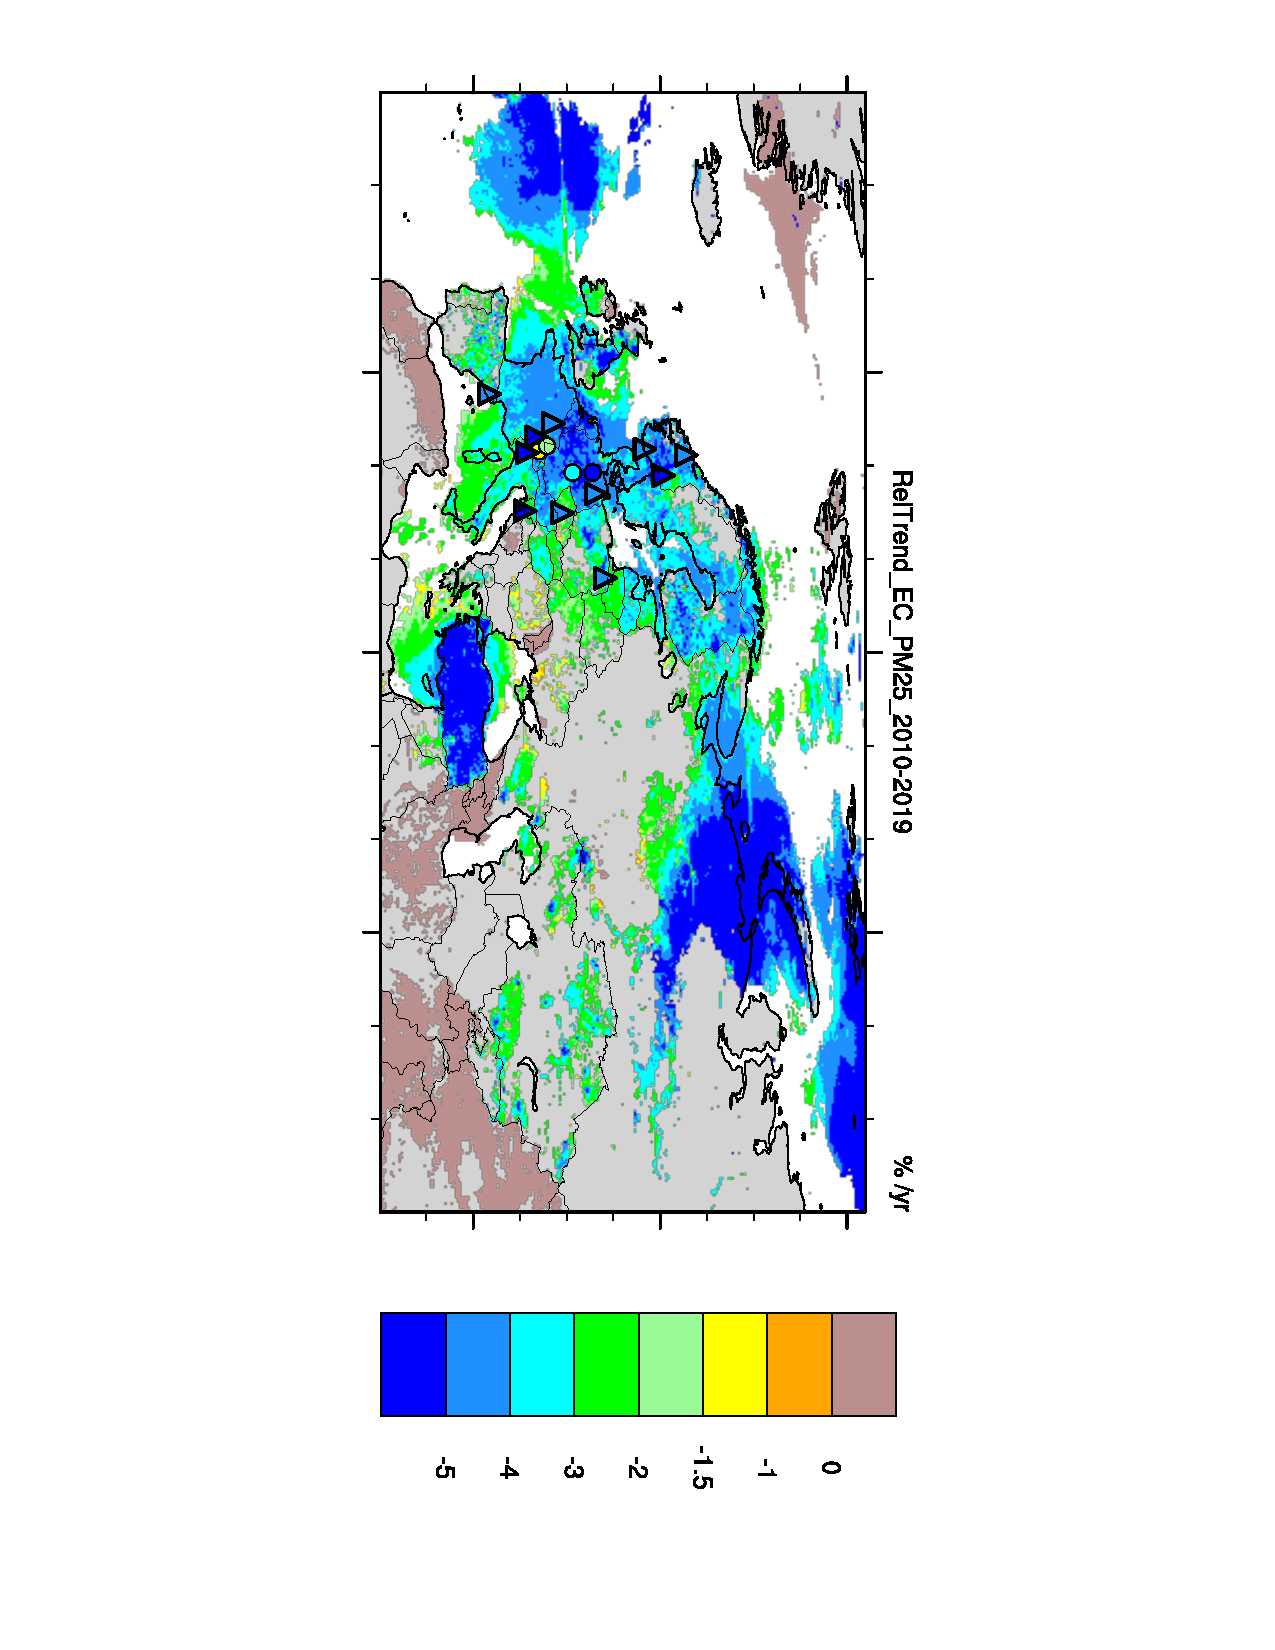
\includegraphics[clip=,angle=90,height=6.1cm,viewport=175 67 448 754]{FIGS_TRENDS/RelTrend_EC_PM25_2010-2019_Perc.pdf}}\\
%  \vspace{0.5cm}
\centering{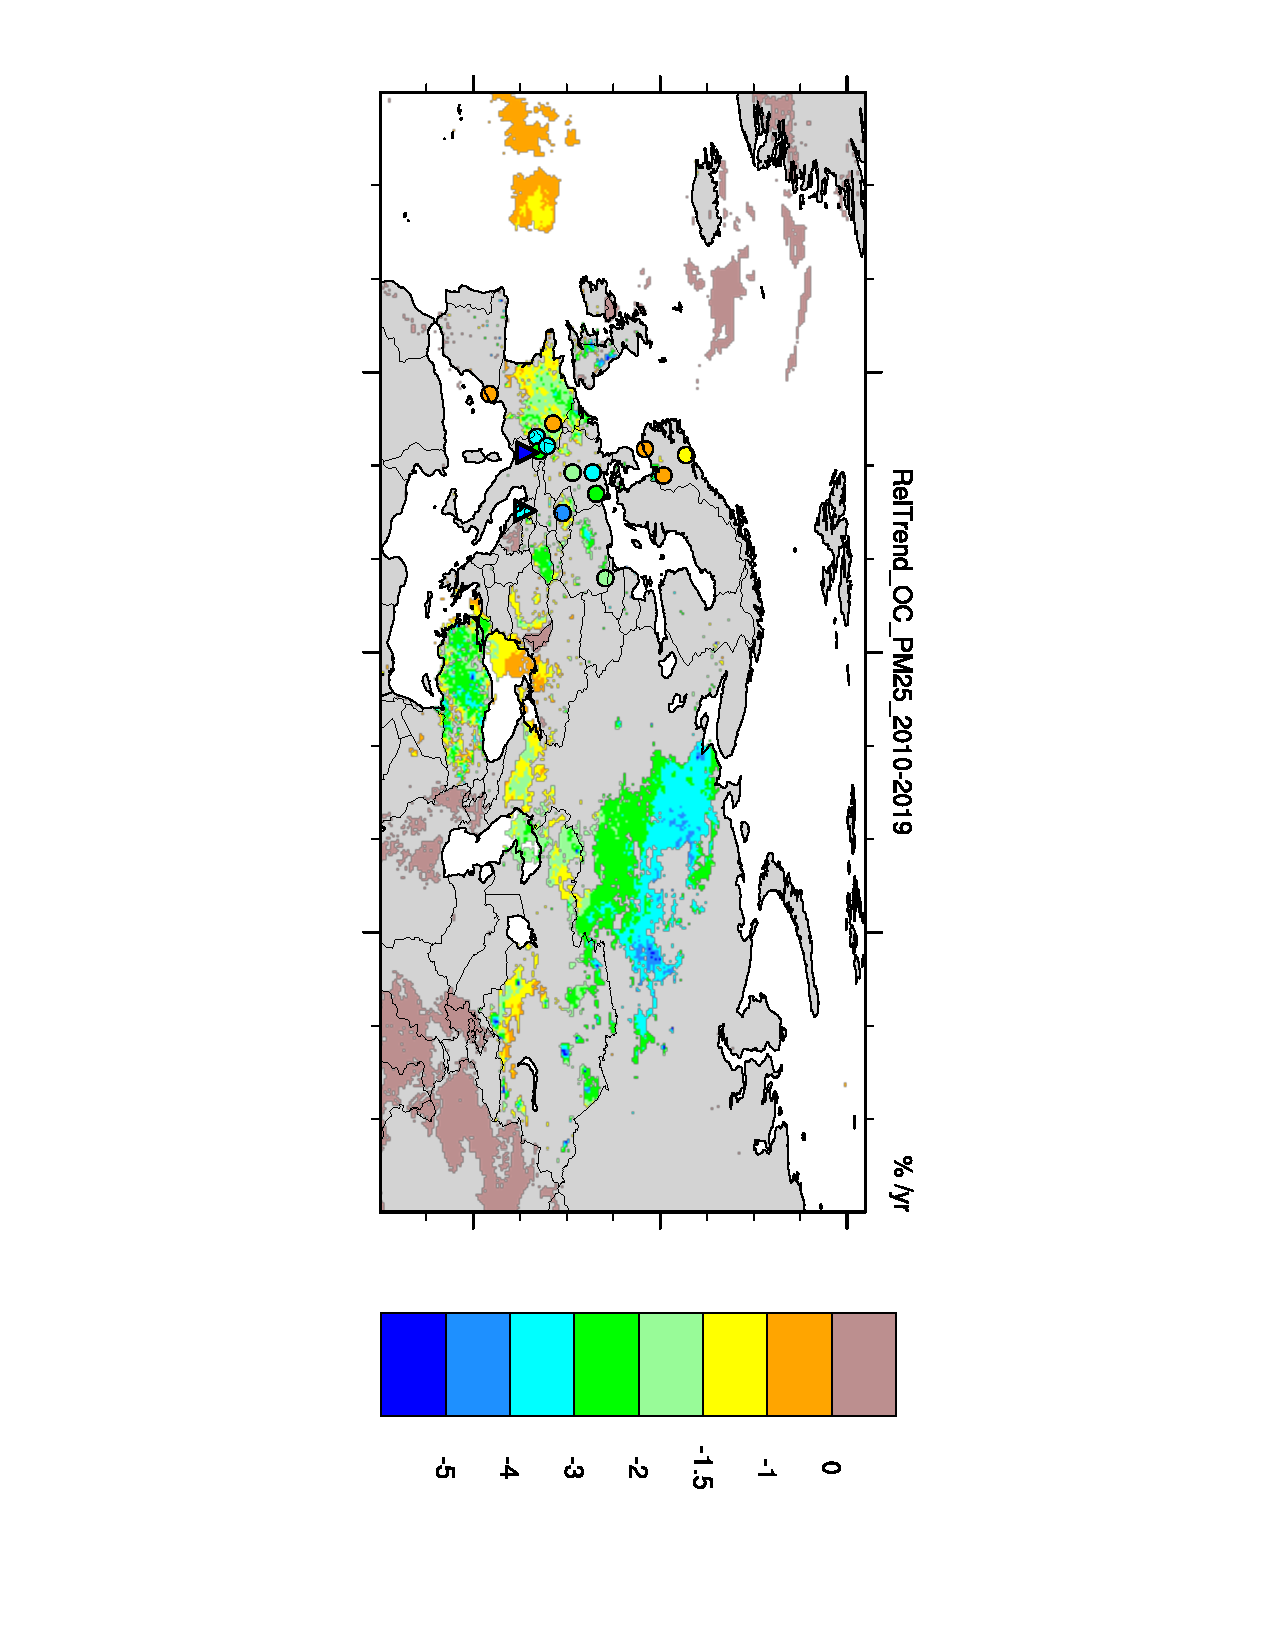
\includegraphics[clip=,angle=90,height=6.1cm,viewport=175 67 448 754]{FIGS_TRENDS/RelTrend_OC_PM25_2010-2019_Perc.pdf}}
\caption{Relative trends for OC in \pmfine over the period of 2010-2019: EMEP modelled -- coloured contours (grey/white means non-significant trends) and observed - coloured triangles (significant) and circles (non-significant).}
\label{fig:OCtrends}
\end{figure}
%%%%%%%%%%%%%%%%%%%%%%%%%%%%%%%%%%%%%%%%%%%%%%%%%

\subsection{Discussion of EC, OC trends}
\label{ss:DiscECOC}

Before discussing the trends shown in Sect.~\ref{ss:trendsEC}-\ref{ss:trendsOC} in  more detail, it is important to note that ten years is a short period over which to assess such trends. In order to illustrate this, Table~\ref{tab:BirkenesTrends} shows trends assessed for three periods, 2008-2018, 2008-2019, and 2010-2019, all using the same methodology. It is seen that the magnitude of the trends can differ substantially depending on the time-window. For EC the values range from -2.2~\%/yr to \mbox{-4.24~\%/yr}, and for levoglucosan from -2.5~\%/yr to -5.2~\%/yr, with all values satisfying the p-value$<$0.05 significance test. Trend values for OC vary even more, but these trends were insignificant for all periods. Although we expect some of these trends to reflect changes in emissions, meteorological variation will also play a large role, especially in causing the high sensitivity of the calculated trends to small changes in the time window chosen.


\begin{table}[H]
\centering
\parbox{11.9cm}{
\caption{Relative trends (\%/yr) (and p-values in parentheses) calculated for Birkenes 
    using different time-windows \label{tab:BirkenesTrends}}}
\begin{tabular}{lcccc}
\toprule
     &         & 2008-2018$^{(a)}$& 2008-2019     & 2010-2019       \\
\midrule
 & & & & \\
%\multicolumn{5}{c}{Revised from Wenche 26/8/21} \\
EC   & annual  & -3.0 (0.043)        &  -2.21 (0.034)   & -4.24 (0.012) \\
OC   & annual  &  -0.44 (0.876)      &   0.18 (--)$^{(b)}$     & -0.64 (--)   \\
Levoglucosan & annual  & -2.5 (0.043)        &  -2.48 (0.024)   & -5.2  (0.032) \\
& & & & \\
\bottomrule 
\end{tabular}\\
\parbox{11.9cm}{

Notes:
(a) Values for 2008-2018 use same procedure as for 2008-2019 and 2010-2019.
Due to minor screening differences, numbers
differ slightly from results of \citet{Yttri2021}, which had 2008-2018 trends of -4.2~\%/yr for EC and -2.8~\%/yr for levoglucosan;
(b) dash (--) indicates highly insignificant p-value.\\
}
\end{table}


The 2010-2019 reduction of 4.2~\%/yr in observed EC across all seasons is rather dramatic, though as noted above a different choice of time-window might suggest a lower magnitude of changes. 
As discussed in Sect.~\ref{ss:trendsEC} there is only a minor seasonal variability in the reduction of EC. This partly reflects the minor seasonal variability in most EC sources, but it is puzzling since residential heating (in GNFR sector C) should have clear winter maxima. \citet{Yttri2021} found that the reduction in EC
was most pronounced in spring and summer at the Birkenes Observatory in
southern Norway for 2001--2018, arguing that this was due to influence
from less abated sources such as domestic heating in winter and fall. This argument was
supported by a smaller change (-2.8~\%/yr) for the biomass burning
tracer levoglucosan (2008--2018) than for EC (-4.2~\%/yr) (these trend numbers are from \citeauthor{Yttri2021}, and differ slightly from trends calculated for this report, c.f. Tab.~\ref{tab:BirkenesTrends}). In this study, however, 
we calculated a -5.2~\%/yr change (i.e. reduction) for the biomass burning tracer
levoglucosan observed at the Birkenes Observatory for 2010-2019, which is
greater than the -4.2~\%/yr change calculated for EC.
%, which might suggest that abatement of carbonaceous aerosol from biomass burning has been equally successful as that of EC from fossil fuel sources. This 
This finding seems to contradict the conclusion made
by \citet{Yttri2021}, but the differences in trends using different time-windows (c.f.Tab.~\ref{tab:BirkenesTrends}) suggests it is difficult to draw firm conclusions about these changes.


As the biomass burning emissions observed at the
Birkenes Observatory is largely long-range transported from Continental
Europe and Western Russia \citep{Yttri2021}, our findings for Birkenes
are likely to be representative for a larger part of Europe. However,
changing footprints  for the Birkenes site may also affect both the trends and
the relative contributions of biomass burning and residential wood combustion (RWC).
Figure~\ref{fig:gnfrCtrends} shows that for some countries, for example France, GNFR C \pmfine emissions have been in constant decline throughout the 2000s. Declines are seen in other countries from around 2010 onwards also. Thus, abatemement of RWC emissions seem to be progressing for many countries within the Birkenes footprint area, though the magnitude of the contribution from different countries will of course vary from year to year.

The issues with condensable organics (Sect.~\ref{ss:IssuesECOC}) impact these estimates of \pmfine emissions and their trends also, and Figure~\ref{fig:gnfrCtrends} is a good illustration of this. France is a country which includes condensables, and Germany is one that does not \citep{CONDws2020}. This difference is a major reason for the magnitude of the French GNFR C emissions compared to those of the more highly populated Germany. 




We can note that \citet{Yttri2021} also found a statistically significant trend of similar magnitude and sign
(-4.2~\%/yr)  for EC for 2010--2019 as for 2001--2018
for the Norwegian Birkenes Observatory. As this site has a footprint that covers{\it ibid.}), this consistency suggests a large-scale reduction in EC emissions over the ten years.

\SKIP{Influenced by
major anthropogenic emission regions in Europe, this finding indicates a
potential for further reductions in future years not only at the Birkenes
Observatory but for Europe in general.  The model calculated a reduction
in EC of -3.9~\%/yr considering all sites, which was slightly less than
for the observations (-4.5~\%/yr) but highly comparable. In spring,
the model-calculated reduction equaled that based on observations,
whereas it was lower for the other seasons. As for the observations,
the model predicted a reduction in EC for all sites, but for a few sites
the model estimated a reduction that was 3--4 times larger than seen
for the observations.
}   % END SKIP

\begin{figure}
    \centering
    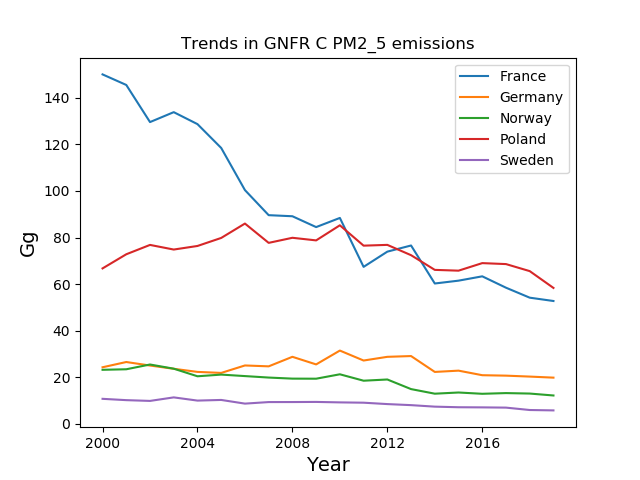
\includegraphics[width=12cm,trim=0 0 0 1.5cm,clip]{FIGS_TRENDS/PlotEmisTrends_PM2_5.png}
    \caption{Trends in \pmfine emissions from GNFR C (mainly residential heating)}
    \label{fig:gnfrCtrends}
\end{figure}

 

Unlike EC, the observed seasonal trends for OC (c.f. Fig.~\ref{fig:KEX1} are very variable, with strong (ca. 4~\%) reductions in the winter months (both DJF and SON), and apparently no change in summertime. As already noted, the individual sites show a great variation in even the sign of the calculated trends, though statistically the trends are not significant (c.f.Fig.~\ref{fig:OCarrows}. The lack of clear trend in summertime is not surprising. 
OC has a substantial influence from
natural sources, biogenic secondary organic aerosol (BSOA) and primary
biological aerosol particles (PBAP), which prevail in the growing season \citep[e.g.][]{Gelencser:CARB,Yttri2019}.
These biogenic emissions are not subject to abatement, but are very sensitive to meteorology, and thus summer-time OC trends are strongly influenced by year-to-year changes in meteorological conditions.

Anthropogenic OC emissions
are likely best represented by winter-time data, and in DJF the observed trend of -4~\%/yr for OC is rather similar to that found for EC (Tab.~\ref{tab:KEX2}). As
for EC, domestic heating is an important emission source 
%Increased emissions from domestic heating are seen
all over Europe in the heating season
\citep[e.g.][]{Yttri2019}, but especially where RWC is utilised.
%when the contribution from natural sources
%is low, and is generally assumed to be poorly abated, particularly
%or residential wood burning. Notably, the winter-time reduction in OC
%was similar to that of EC considering all sites, and a
At the Birkenes
Observatory the winter-time reduction in OC (-4.1~\%/yr) was only somewhat
lower than for EC (-6.4~\%/yr) and levoglucosan (-4.6~\%/yr).
\SKIP{
  Karl Espen - where are these numbers coming from? Different to those in Tab.~\ref{tab:BirkenesTrends}
}
These results also suggest
that abatement of residential wood burning emissions has been quite
effective for Europe in general, taking into account the considerations
made about the length of the time series and the Birkenes Observatory as
an indicator of European emissions (Sect.~\ref{ss:trendsEC}).  

The underprediction of the OC levels in wintertime seen in Figs.~\ref{fig:KEX1} should not be taken as a indication that the EMEP model itself is wrong, but is rather at least partly the result of the issues with missing `condensable' organics (Sect.~\ref{ss:IssuesECOC}). It has been demonstrated elsewhere that model results improve substantially when condensables are included \citep{DeniervanderGon2015,R2019:SVOC,R2020:SVOC}. Unfortunately, we do not yet have a time-series of condensable organic emissions with which to perform trend analysis, but we hope to address that within the context of a new MSC-W led project funded by the Nordic Council of Ministers.

\SKIP{
A pronounced influence of natural sources in areas
less perturbed by anthropogenic emissions, exemplified by Scandinavia,
is a possible explanation \citep{Bergstrom2012,Yttri2021}, although a
less successful abatement of anthropogenic sources cannot be excluded.
}

%%%%%%%%%%%%%%%%%%



\subsection{OC and EC fractions of PM}
\label{ss:OCECfrac}


\begin{figure}
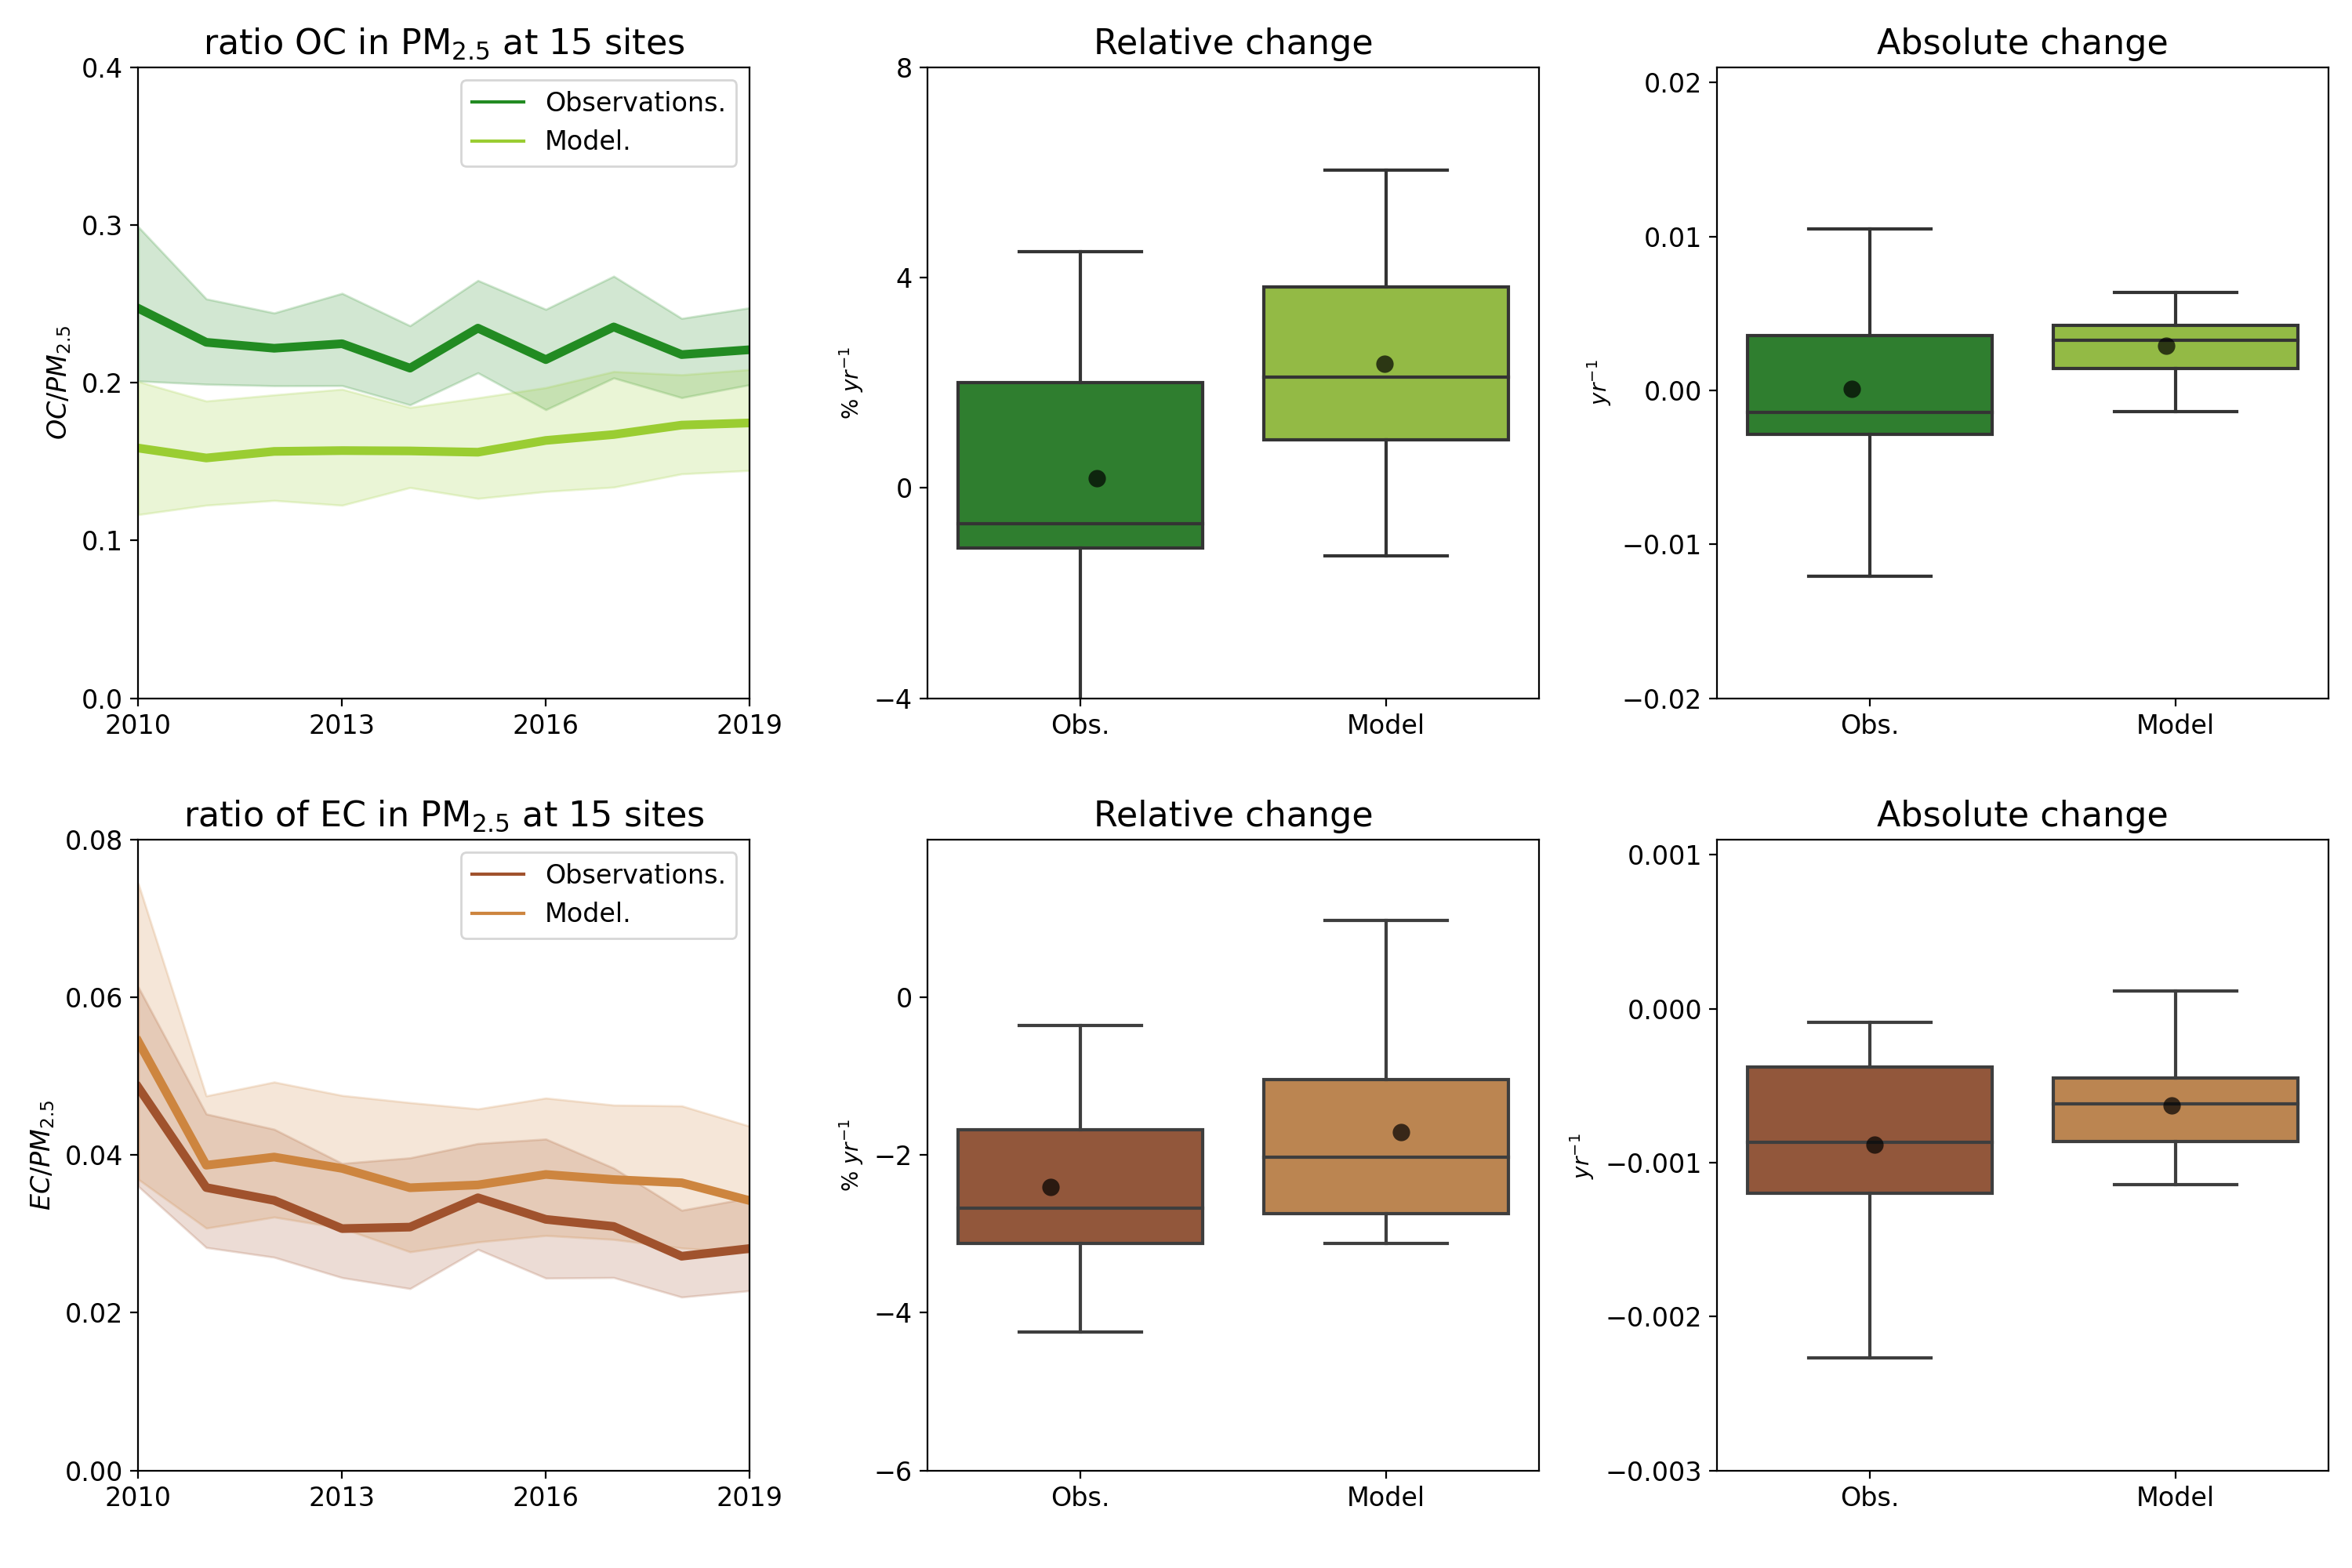
\includegraphics[width=16cm]{FIGS_TRENDS/ECOC_ratio_trends.png}
 \caption{Observed and modelled ratios and trends of OC/\pmfine and EC/\pmfine for
  15 EMEP sites across Europe for 2010--2019, showing the trends
  (left panels) of OC/\pmfine (upper) and EC (lower), aggregated annual and
  seasonal relative changes (mid panels) for OC (upper) and EC (lower),
  and aggregated annual and seasonal absolute changes (right panels)
  for OC (upper) and EC (lower). The solid line in the left panel shows
  the average annual mean for all sites and the shaded area the 95\%
  confidence interval. For explanation of the statistics in the figure,
  see Fig.~\label{fig:KEX3}
 }
\end{figure}

As focused abatement of anthropogenic secondary inorganic aerosol (SIA)
precursors have reduced ambient SIA levels substantially (Sects.~\ref{sec:Trends_sulfur}--\ref{sec:Trends_reduced nitrogen }), 
other, non-SIA fractions are likely to contribute an increasing fraction
of PM. For the EC fraction of \pmfine, however, there was a reduction,  -2.4$\pm$1.1~\%/yr, 
for 2010--2019 (Fig.~\ref{fig:KEX3}, Tab.~\ref{tab:KEX3}), showing that EC has been
more efficiently abated than the overall PM mass concentration. The model
calculated a comparable reduction (-1.7$\pm$1.3~\%/yr) for the EC/\pmfine ratio
but predicted a minor increase at two of the sites, which was not seen for
observed EC/\pmfine ratios. For the few sites where measurements allow for
a harmonized data set of EC, OC, \ce{SO4^2-} and \pmfine, i.e., only including
measurements on common days, the reduction in the EC fraction of \pmfine
was typically equally high or higher than for the \ce{SO4^2-} fraction. The
OC fraction of \pmfine showed no decrease or increase (0.2$\pm$2.8~\%/yr)
for 2010--2019 when considering all sites, which largely is explained by
non-abatable natural sources making up a major part of OC. A substantial
4.5~\%/yr increase in OC/\pmfine was calculated for the Norwegian sites,
experiencing low (anthropogenic) aerosol levels and a high OC fraction
from natural sources, thus one cannot exclude the possibility that part
of this increasing trend is due to an increase in natural sources and
not exclusively from a decrease in anthropogenic emissions. A 2.8~\%/yr
increase in the OC fraction was observed for the Spanish site Montseny,
resembling the Norwegian sites with respect to a low aerosol level and
a high OC fraction from natural sources \citep{Kulmala2011,Crippa2014}. For the
rest of continental Europe, a minor $\pm$1~\%/yr increase/decrease
was seen at most sites and a $\pm$2~\%/yr for a few. The Kosetice
(Czech Republic) (-5.3~\%/yr) and Shauinsland (Germany) (-3.1~\%/yr) sites
experienced a substantial decrease in the OC fraction, which was larger
than the corresponding decrease in the EC fraction, thus deviating from
the pattern seen at all other sites where the decrease in EC/\pmfine $>$
OC/\pmfine.

\begin{figure}
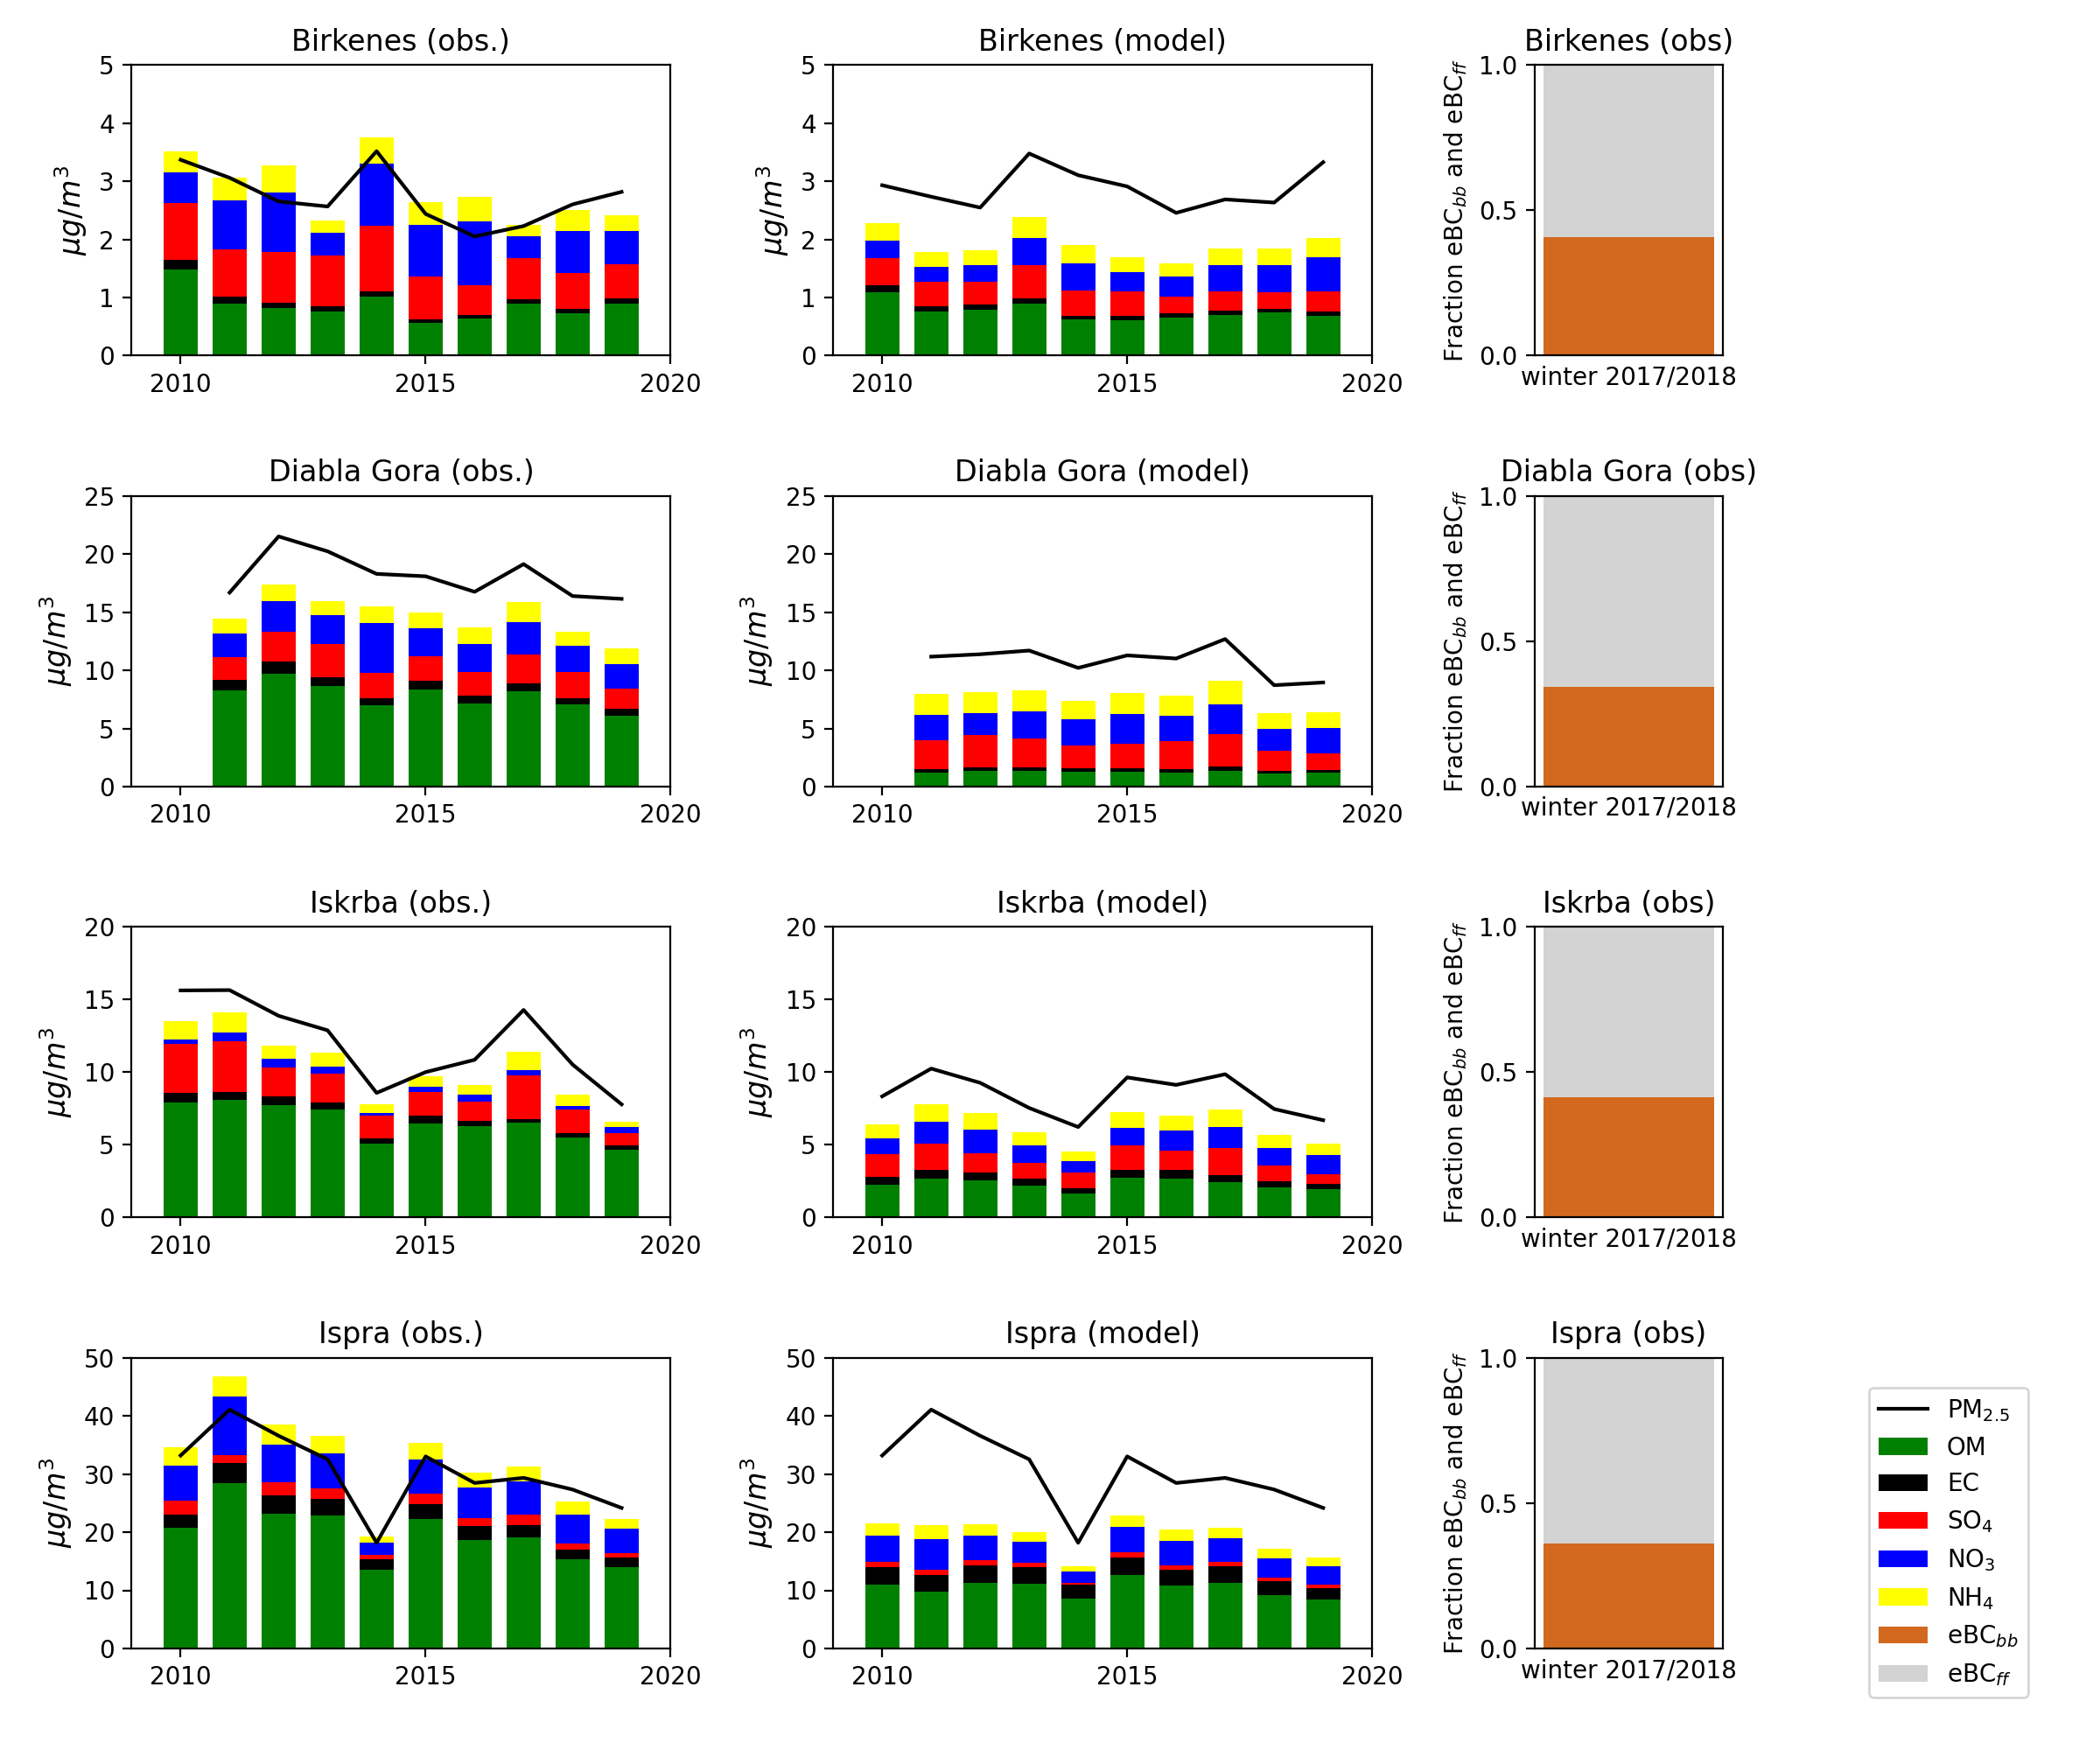
\includegraphics[width=16cm]{FIGS_TRENDS/Compostion_4sites_winter.png}
 \caption{
  Mass balance of wintertime \pmfine at  Birkenes (NO02), Diabla Gora
  (PL05), Iskrba (SI08) and Ispra (IT04) including OM, EC, \ce{SO4^2-}, \ce{NO3^-}, \ce{NH4^+} from 
  observations (left), modelled (middle) and apportionment of eBC
  into biomass burning/solid fuel (\EBCff) and fossil fuel/liquid fuel
  (\EBCbb) for winter 2017/2018 (right). Note that at NO02 and PLO5 the SIA components in observations are from filterpack sampler with no cutoff and probably overestimate the \pmfine SIA. \label{fig:KEX4}
 }
\end{figure}


The relative contribution of carbonaceous aerosol, OM (assuming OM = OC $\times$
1.4 for Ispra
\footnote{The lower factor is needed for Ispra to keep mass balance $\le$100\%.}
and 1.7 for the other sites)
 and EC, to the \pmfine mass concentration along with the major
SIA species illustrates the importance of the OM fraction for a further
reduction in wintertime \pmfine mass concentration (Fig.~\ref{fig:KEX4}). As a first step,
the natural and the anthropogenic fraction of the carbonaceous aerosol
must be separated, then further into abatable categories. Separation of
eBC into biomass burning/solid fuel (\EBCbb) and fossil fuel/liquid fuel
(\EBCff) is possible using data from the multi wavelength aethalometer,
currently available at $<$25 EMEP/ACTRIS sites across Europe \citep{Yttri:2014,Platt:2020a,Platt:2020b,Platt20XX}. An obvious next
step is to implement such analysis as part of regular monitoring,
making it possible to validate not only model performance, but also the
effort made in reducing carbonaceous aerosol from fossil fuel and biomass
burning sources. Although not directly comparable to the multi-year plots
presented in Fig.~\ref{fig:KEX4}, results from the EIMPs Winter 2017/2018 nicely
illustrates the split between \EBCbb and \EBCff for winter 2017/2018 for
the Italian site Ispra, (IT04), the Norwegian site Birkenes (NO02), the
Polish site Diabla Gora (PL05) and the Slovenian site Iskrba (SI08). The
apportionment of eBC can also be used to infer the corresponding fractions
of OM.

\begin{table}
\centering
\parbox{14cm}{
 \caption{
   Absolute and relative change and the corresponding 95\% confidence intervals in observed and modelled annual and seasonal    aggregated OC/\pmfine and EC/\pmfine ratios at 15 sites across Europe
   for 2010--2019. The number of sites with a significant outcome is provided.\label{tab:KEX3}
 }}
 \scalebox{0.95}{%
 \begin{tabular}{lcccccc}
\hline  % toprule
 &  &  &  &  &  &  \\
\multicolumn{7}{c}{EC/\pmfine (2010--2019)} \\
  &  &  &  &  &  &  \\
  \hline
     \multicolumn{3}{c}{Number of sites} & \multicolumn{2}{l}{Absolute change (\ugC/yr)} & \multicolumn{2}{l}{Relative change (\%/yr)} \\
{} &           total & sign. &                     abs &       Conf. interv. &                      \%/y &   Conf. interv. \\
%How   &                 &       &                         &                     &                          &                 \\
\hline  % midrule
Model &              15 &     5 &                 -0.0006 &  (-0.0009, -0.0004) &                    -1.71 &   (-2.32, -1.1) \\
Obs.  &              15 &     4 &                 -0.0009 &  (-0.0012, -0.0006) &                    -2.41 &  (-2.96, -1.85) \\
\hline  % bottomrule
% \end{tabular}
   &  &  &  &  &  &  \\
\multicolumn{7}{c}{OC/\pmfine (2010--2019)} \\
   &  &  &  &  &  &  \\
% \begin{tabular}{lrrrlrl}
\toprule
   \multicolumn{3}{c}{Number of sites} & \multicolumn{2}{l}{Absolute change (\ugC/yr)r} & \multicolumn{2}{l}{Relative change (\%/yr)} \\
{} &           total & sign. &                     abs &     Conf. interv. &                      \%/y &  Conf. interv. \\
%How   &                 &       &                         &                   &                          &                \\
\hline  % midrule
Model &              15 &     7 &                  0.0029 &   (0.0018, 0.004) &                     2.35 &     (1.3, 3.4) \\
Obs.  &              15 &     2 &                  0.0001 &  (-0.003, 0.0032) &                     0.19 &  (-1.24, 1.62) \\
\hline  % bottomrule
\end{tabular}
} % end scalebox
\end{table}




\subsection{Trends in EC and OC, conclusions}
\label{ss:trendsECOCconc}

For EC and OC we have calculated observed and modelled trends for 15 sites across Europe for the period 2010--2019. It should be noted that this 10-year period is rather short for the calculation of robust trends (and we show that slightly different time-windows produce different statistics), and typically only a limited number of sites showed trends that were statistically significant for specific seasons, even for a specific time-window. However, some features of the trend analysis seem rather consistent, and we summarise the main points here. 

A reduction (of ca. 4.5~\%/yr) in observed EC was found across 15 sites across Europe for the  period 
2010--2019. The reduction in levoglucosan at the site Birkenes in southern Norway (which is significantly impacted by long-range transport of pollution from continental Europe) was found to be over 5\% also (though this number was very sensitive to the time-window), which suggests that emissions from residential wood combustion were reduced significantly over this period; this is also consistent with reported changes in the GNFR C emissions from some countries at least. However, observed EC reduction levels were rather similar in all seasons, which suggests that emissions abatement of EC has been successful across a range of emission sources. 

In the winter season (DJF), reductions in observed EC and OC were very similar, with \mbox{-4.3~\%/yr} and -4.2~\%/yr respectively. Given that the winter OC concentrations are mainly determined by primary emissions and with minimal SOA contributions, this consistency of EC and OC reductions is also consistent with reductions in wintertime anthropogenic sources. Trends in observed OC in other seasons were however very mixed, with some stations showing increases, and others decreases, and with little statistical significance. This variability in station-to-station OC trends in other seasons reflects increasing contributions from SOA formation, which are sensitive to meteorological factors and biogenic emissions.

The modelled trends in EC (reduction of ca. 4~\%/yr) were rather similar to the observed trends, also across all seasons, and the station-mean EC concentrations themselves were well reproduced by the model across the 10 year period. 
For OC, the model substantially underpredicts the yearly concentrations over the whole period, and also underpredicts the trends.  

The underprediction of OC may partly be due to general difficulties with modelling SOA formation, but a major problem is the omission of condensable organics in the reported \pmfine emissions from many countries (Sect.~\ref{ss:IssuesECOC}). Although emissions estimates which include condensables (the so-called REF2 or REF2.1, Sect.~\ref{sec:EmisSVOC}) are available and were used in the status and source-receptor calculations of this report, these emissions only exist for 2015; no time-series of REF2-type emissions yet exists. The lack of significance of the calculated OC trends may also be attributed to some extent to these problems with condensables. When some countries include, and some exclude, condensables, changes in modelled OC concentrations will be very sensitive to changes in the source areas for the primary OC emissions entering the model.
Although modelling of EC is also impacted by the problems with condensables (due to the use of OC/EC ratios when interpreting \pmfine emission speciation, see Sect.~\ref{ss:IssuesECOC}), the much better agreement found for wintertime EC levels than for OC probably reflects the fact that EC has a wider variety of emission sources in that season (e.g. vehicles) than OC, which is much more dominated by residential wood-burning.


The EC fraction of \pmfine  decreased at all
sites (average of -2.4$\pm$1.1~\%/yr), and at a level equal to, or higher than, the \ce{SO4^2-} fraction. The
change in OC fraction was more scattered with a substantial and
consistent 4.5~\%/yr increase at the northernmost sites, whereas
there was no increase or decrease (0.2$\pm$2.8~\%/yr) when considering
all sites. The influence of OC from natural sources likely has a profound
impact on the general lack of decrease observed for the OC fraction of
\pmfine. These observations points to a continuous change in the aerosol
chemical composition and in the relative source composition across
Europe. The carbonaceous fraction appears particularly important for a
further reduction in the observed \pmfine mass concentration in Europe,
although effort is needed to separate its natural and anthropogenic
fraction to get a quantitative overview of the abatable fractions.
\\
\bigskip


\SKIP{ % COMMENT{\bigskip ORIG TEXT, DELETE if above is okay:\\}

A -4.5$\pm$1.6~\%/yr reduction in EC was calculated across Europe for
2010--2019 and the reduction was particularly consistent amongst the
sites where the reduction was statistically significant. The model
predicted a reduction that was somewhat lower (-3.9~\%/yr) than the
observations, but still comparable. A similar reduction in EC (-4.2~\%/yr)
was calculated for 2010--2019 as for 2001--2018 at the Birkenes
Observatory in southern Norway. This consistent reduction indicates a
potential for further reduction in future years for Europe in general,
as LRT from continental Europe explains most EC from both fossil fuel
and biomass burning sources at the Birkenes Observatory. A  -5.2~\%/yr
reduction in levoglucosan at the Birkenes Observatory (2010--2019)
 indicate that EC from wood burning in Europe is declining equally
rapid as that of EC from fossil fuel sources.

The reduction in OC (-2.4$\pm$1.6~\%/yr) was less pronounced than for EC,
whereas winter-time levels (-4.2~\%/yr) were comparable to EC. Non-abatable
natural sources of OC peak in the growing season diluting anthropogenic
sources, thus, anthropogenic OC emissions are likely best represented by
winter-time data. Comparable reductions in winter-time OC (-4.1~\%/yr),
winter-time EC (-6.4~\%/yr) and winter-time levoglucosan (-4.6~\%/yr)
at the Birkenes Observatory suggest that abatement of residential
wood burning emissions has been quite effective for Europe in general,
taking into account considerations about the length of the time series
and Birkenes as an indicator of European emissions.

The model calculated a reduction in OC of -0.6~\%/yr, being noticeable
less than for the observations (-2.4~\%/yr). A similar underprediction
was seen for each season, thereby reproducing the seasonality in trend
seen for the observations.

The EC fraction of \pmfine decreased at all
sites (-2.4$\pm$1.1~\%/yr), and at a level equal to, or higher than, the \ce{SO4^2-} fraction. The
change in OC fraction was more scattered with a substantial and
consistent 4.5~\%/yr increase at the northernmost sites, whereas
there was no increase or decrease (0.2$\pm$2.8~\%/yr) when considering
all sites. Influence of OC from natural sources likely has a profound
impact on the general lack of decrease observed for the OC fraction of
\pmfine. These observations points to a continuous change in the aerosol
chemical composition and in the relative source composition across
Europe. The carbonaceous fraction appears particularly important for a
further reduction in the observed \pmfine mass concentration in Europe,
although effort is needed to separate its natural and anthropogenic
fraction to get a quantitative overview of the abatable fractions.\\
}


\SKIP{ % Now moved to ExecSummary
For EC and OC we have calculated observed and modelled trends for 15 sites across Europe for the period 2010--2019. A reduction (of ca. 4.5~\%/yr) in observed EC was found, and a similar reduction was found for OC in the winter months (when OC is expected to be most sensitive to primary anthropogenic emissions rather than to OA associated with biogenic sources). These trends suggest that abatement measures are having some success in reducing both EC and OC in Europe, especially in wintertime.  The model reproduced modelled EC values and trends quite well, but underpredicted OC, both in terms of absolute values and trends. This underprediction is at least partly due to the omission of condensable organics in the reported emissions from many countries. 
%
The carbonaceous fraction appears particularly important for a
further reduction in the observed \pmfine mass concentration in Europe,
although effort is needed to separate its natural and anthropogenic
fraction to get a quantitative overview of the abatable fractions.
}


\clearpage
\section{Exceedances of critical loads of acidification and eutrophication in 2000 to 2019.}
\label{subs:exceedSnN}
%Thomas/CCE: I just updated this section. Please have a look TS 17.08.2021

The exceedances of European critical loads (CLs) are computed for the total nitrogen
(N) and sulphur (S) depositions modelled on the 0.1$\degrees \times$ 0.1$\degrees$
longitude-latitude grid (approx. 11 x 5.5 km$^{2}$ at 60$\degrees$N).
Exceedances are calculated for the European critical loads documented in \cite{Hettelingh:2017}, while
a description of the methods is given in \cite{DeVries:2015}. The
critical loads data for eutrophication by N (CL eut N) and for acidification by N and S
(CL acid) are also used by the EMEP Centre CIAM (located at IIASA) in their integrated assessment
modelling. The exceedance in a grid cell is the so-called ’average accumulated
exceedance’ (AAE), which is calculated as the area-weighted average of the
exceedances of the critical loads of all ecosystems in this grid cell. The units for
critical loads and their exceedances are equivalents (eq; same as \textit{moles of charge},
molc) per area and time, making S and N depositions comparable on their impacts, which is important for
acidity CLs.

Critical loads are available for about 4 million ecosystems in Europe covering an area
of about 3 million km$^{2}$ (west of 42$\degrees$E). The exceedances (AAE) of those critical loads
are computed on a 0.1$\degrees \times$ 0.1$\degrees$ longitude-latitude grid, and maps for the deposition in
the years 2000, 2005, 2010, 2015 and 2019 are shown in Figures \ref{fig:eutN} and \ref{fig:acid}. As indicated in the maps, the critical loads for eutrophication are exceeded in practically all countries in all years. The share of ecosystems where the critical load for eutrophication is exceeded decreases relatively slowly, starting at 76.4\% in 2000 and ending at 65.5\% in 2019.
European average AAE is about 452 eq ha$^{-1}$ yr$^{-1}$ (2000) and 276 eq
ha$^{-1}$ yr$^{-1}$ (2019). The highest exceedances of CLs are found in the Po Valley in Italy, the
Dutch-German-Danish border areas and in north-eastern Spain.
By contrast, critical loads of acidity are exceeded in a much smaller area. Hot spots of
exceedances can be found in the Netherlands and its border areas to Germany and
Belgium, and some smaller maxima in southern Germany and Czechia,
whereas most of Europe is not exceeded (grey areas). Acidity exceedances occur
on 16.2\% (2000) and 5.0\% (2019) of the ecosystem area and the European average
AAE is about 133 eq ha$^{-1}$ yr$^{-1}$ (2000) and 25 eq ha$^{-1}$ yr$^{-1}$ (2019). Overall statistics for the share of critical load exceedance and European average of AAE are shown in Figures \ref{fig:stats_cl_ex}.
\begin{figure}[ht]
  \centering
  \subfigure{\includegraphics*[scale=0.20]{FIGS_CL_Exceedance/Stats_CLex_eut.png}}
  \subfigure{\includegraphics*[scale=0.20]{FIGS_CL_Exceedance/Stats_CLex_acid.png}}
  \caption{Summary for exceedance of critical load for eutrophication (left) and acidification (right).}
\label{fig:stats_cl_ex}
\end{figure}
\begin{figure}[ht]
  \centering
  \subfigure{\includegraphics*[scale=0.35]{FIGS_CL_Exceedance/CL_Ex_eut_2000.png}}
  \subfigure{\includegraphics*[scale=0.35]{FIGS_CL_Exceedance/CL_Ex_eut_2005.png}}
  \subfigure{\includegraphics*[scale=0.35]{FIGS_CL_Exceedance/CL_Ex_eut_2010.png}}
  \subfigure{\includegraphics*[scale=0.35]{FIGS_CL_Exceedance/CL_Ex_eut_2015.png}}
  \subfigure{\includegraphics*[scale=0.35]{FIGS_CL_Exceedance/CL_Ex_eut_2019.png}}
 \caption{Exceedance of critical load for eutrophication for the years 2000, 2005, 2010, 2015 and 2019.}
\label{fig:eutN}
\end{figure}
\begin{figure}[ht]
  \centering
 \subfigure{\includegraphics*[scale=0.35]{FIGS_CL_Exceedance/CL_Ex_acid_2000.png}}
  \subfigure{\includegraphics*[scale=0.35]{FIGS_CL_Exceedance/CL_Ex_acid_2005.png}}
  \subfigure{\includegraphics*[scale=0.35]{FIGS_CL_Exceedance/CL_Ex_acid_2010.png}}
  \subfigure{\includegraphics*[scale=0.35]{FIGS_CL_Exceedance/CL_Ex_acid_2015.png}}
  \subfigure{\includegraphics*[scale=0.35]{FIGS_CL_Exceedance/CL_Ex_acid_2019.png}}
 \caption{Exceedance of critical load for acidification for the years 2000, 2005, 2010, 2015 and 2019.}
\label{fig:acid}
\end{figure}





%%%%%%%%%%%%%%%%%%%%%%%%%%%%%%%%%%%%%%%%%%%%%%%%%%%%%%%%%%%%%%%%%%%%%%%%%%%%%%%%%%%%%%
\clearpage


\bibliographystyle{copernicus}         % change bibliography-name after each
\renewcommand\bibname{References}      % bibliographystyle command!
\addcontentsline{toc}{section}{References}
%\bibliography{trends,Refs,EMEP_Reports,NILU,RefsUpdates,RefsEmis}
\bibliography{Refs2021}
 %Wenche, Hilde, Svetlana (Jonas/Augustin about how the trends have been calculated)
%\include{chapterTrendsOzone} %Sverre, David, Joffen
%\section{Trends in Elemental and Organic Carbon}
\label{sec:trendsECOC}
\subsection{Elemental Carbon, EC}
\label{ss:trendsEC}


\begin{figure}
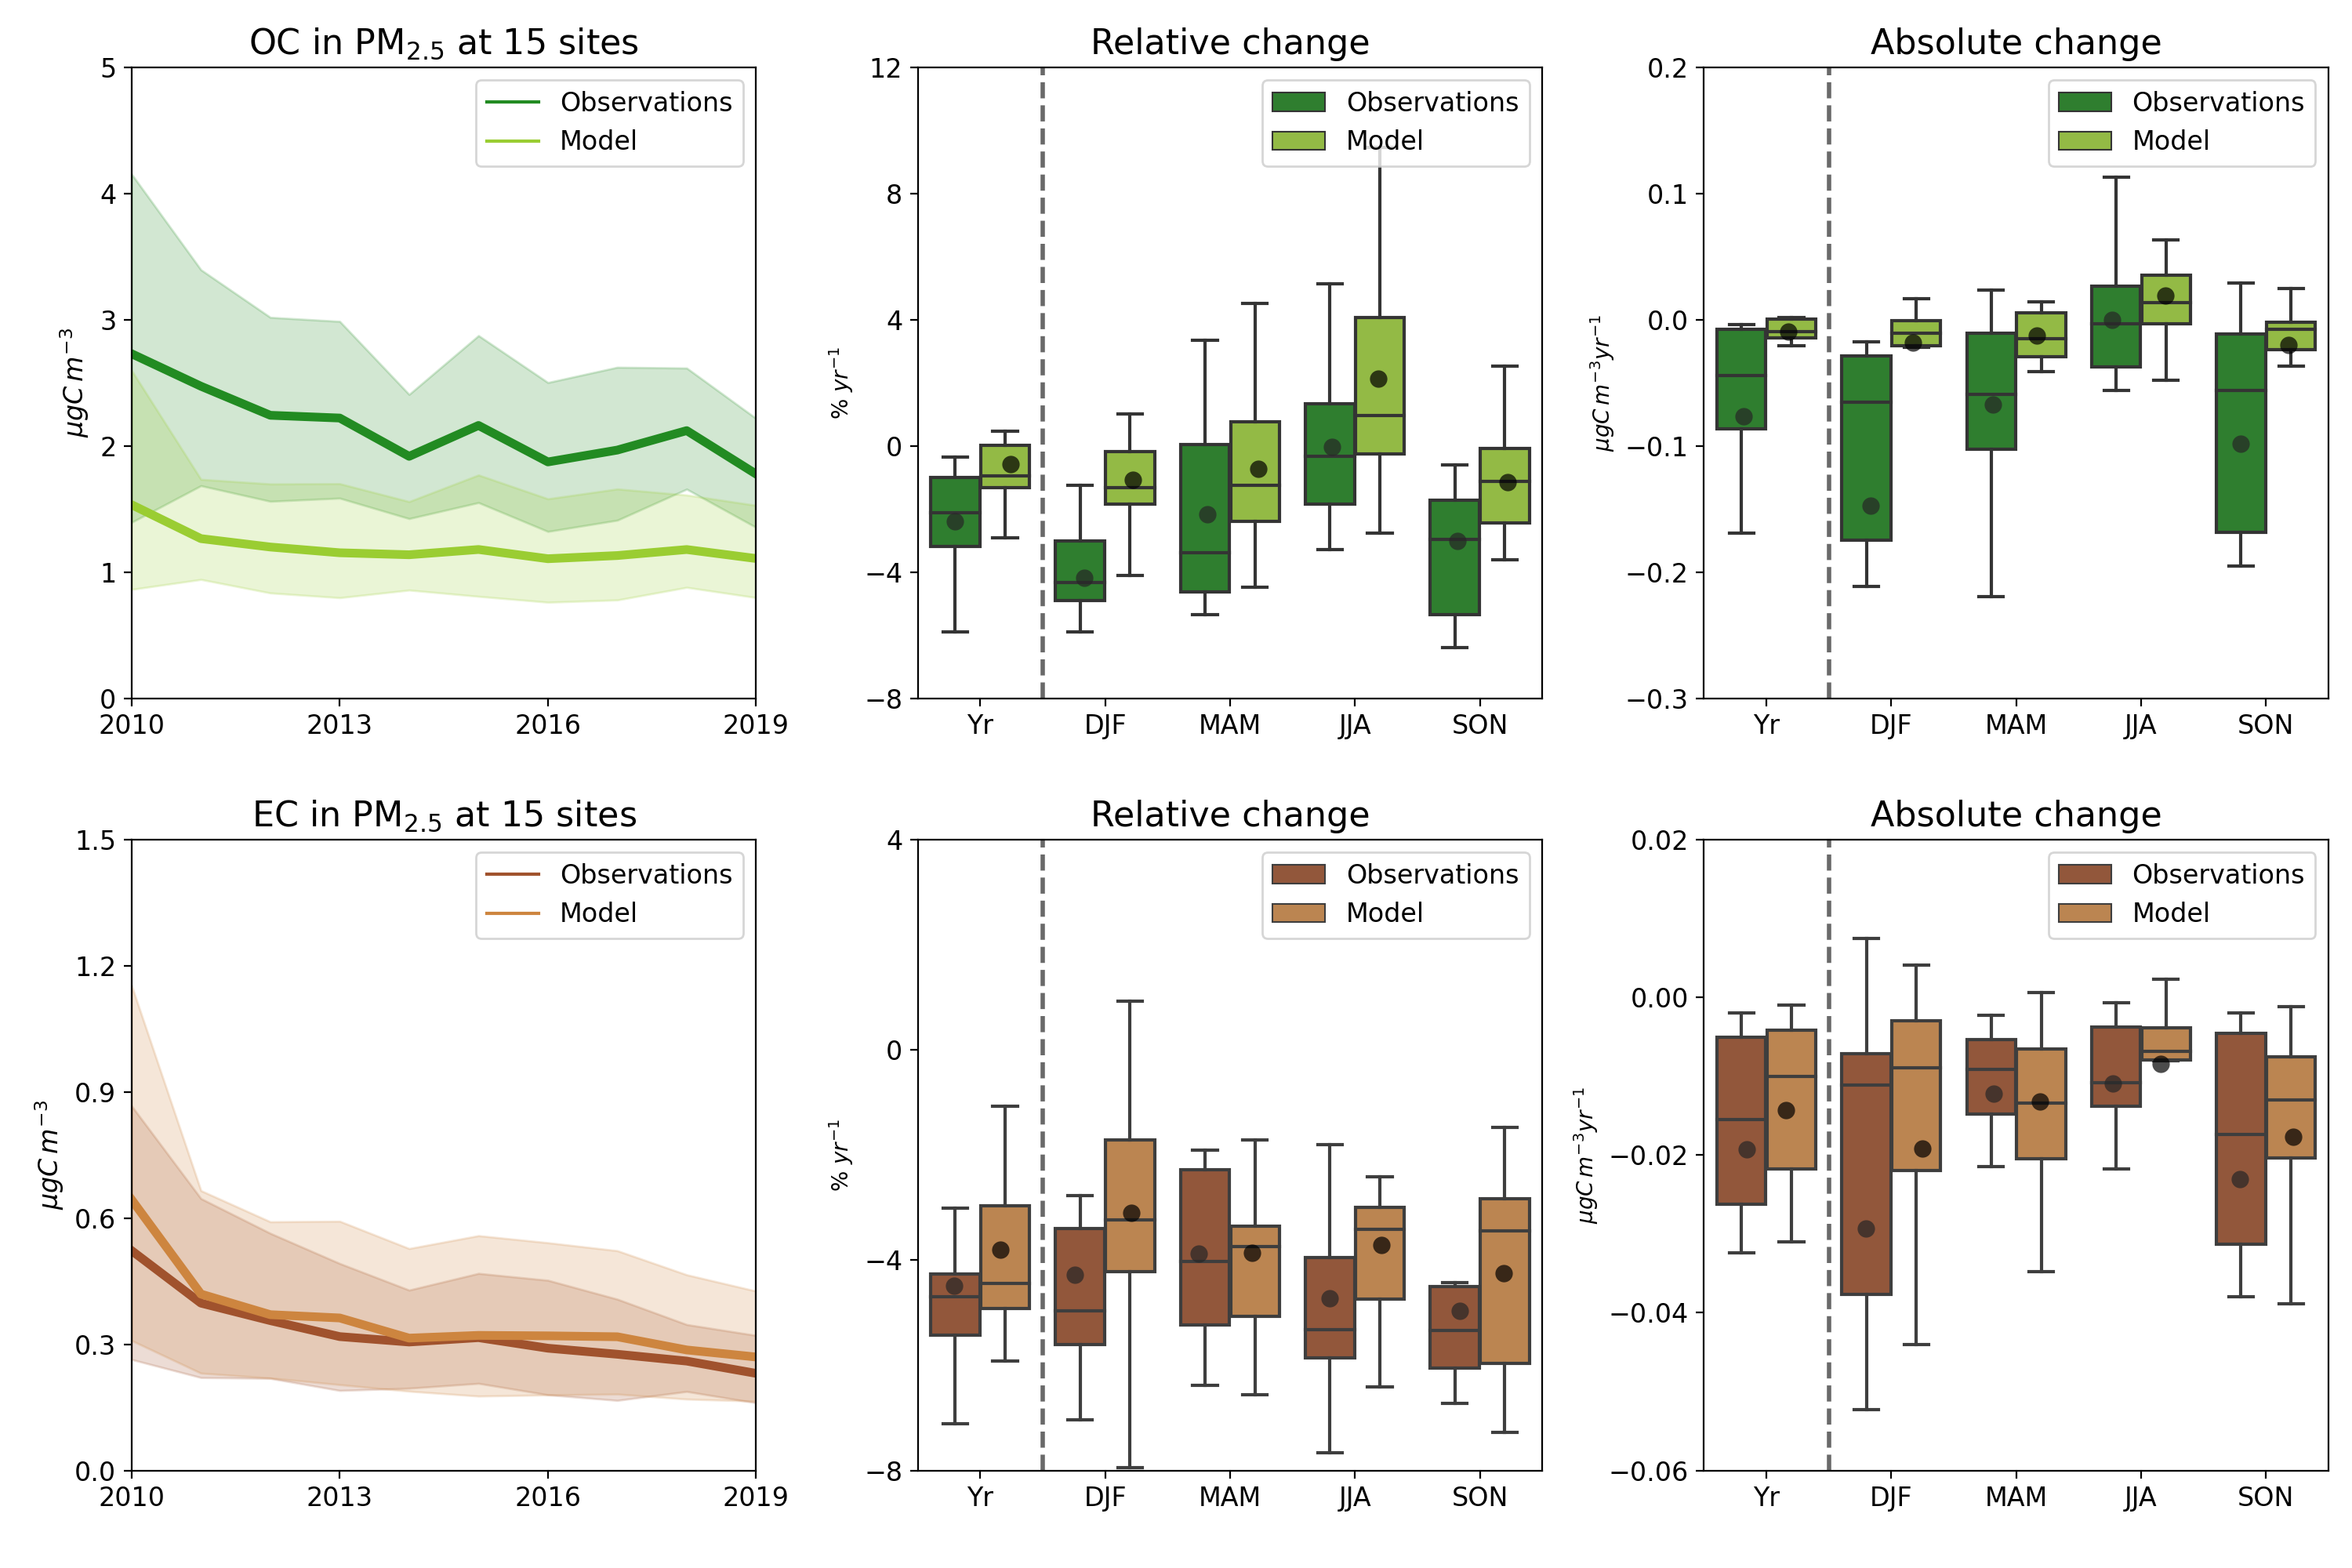
\includegraphics[width=16cm]{FIGS_TRENDS/ECOC_trends.png}
\caption{Observed and modeled concentrations and trends of EC and OC at 15 EMEP
  site across Europe for 2010--2020, showing the concentrations
  (left panels) of OC (upper) and EC (lower), aggregated annual and
  seasonal relative changes (mid panels) for OC (upper) and EC (lower),
  and aggregated annual and seasonal absolute changes (right panels)
  for OC (upper) and EC (lower). The solid line in the left panel shows
  the average annual mean for all sites and the shaded area the 95\%
  confidence interval. The box plots in the mid and right panels show
  the 25th and 75th percentiles (boxes), the median (horizontal lines),
  whereas the whiskers represent the interquartile ranges $\times$
  1.5 and the squares the outliers. Black markers within the box are
  the means.\label{fig:KEX1}
}
\end{figure}

A 4.5$\pm$1.5\%/yr reduction 
 \COMMENT{DS: changed - xx reduction to just xx reduction. Should be careful throughout...}
in elemental carbon (EC) for 2010--2020 was
calculated for the 15 sites assessed (Fig.~\ref{fig:KEX1}, Tab.~\ref{tab:KEX1}),
being quite comparable to the reduction (-5.0$\pm$0.9\%/yr)
calculated for the eleven sites where the reduction was statistically
significant. The reduction was rather similar considering these eleven
sites, ranging from -4.2\%/yr to -5.8\%/yr for ten out of eleven
sites, thus we see no apparent spatial pattern in the reductions
(Fig.~\ref{fig:KEX2}. The largest reduction was seen amongst the sites with the
highest EC levels, i.e., at Iskrba (-7\%/yr) in Slovenia and at Ispra
(-5.8\%/yr) in the Po Valley region in Northern Italy. Notably, these
were the only sites where a statistically significant reduction was
observed for all seasons, being most pronounced in summer, although
by a small margin. When considering all sites, the reduction was most
pronounced in summer and fall (Tab.~\ref{tab:KEX1}), but the general picture is
that there is a minor seasonal variability in the reduction of EC,
reflecting minor seasonal variability in most EC sources, except from
residential heating. \citet{Yttri2021} found that the reduction in EC
was most pronounced in spring and summer at the Birkenes Observatory in
southern Norway for 2001--2018, arguing that this was due to influence
from less abated sources such as domestic heating in winter and fall,
supported by a lower (-2.8\%/yr) reduction for the biomass burning
tracer levoglucosan (2008--2018) than for EC (-4.2\%/yr). Here,
we calculated a -5.2\%/yr reduction for the biomass burning tracer
levoglucosan observed at the Birkenes Observatory for 2010-2020, which is
higher than the -4.2\%/yr calculated for EC, suggesting that abatement
of carbonaceous aerosol from biomass burning has been equally successful
as that of EC from fossil fuel sources, contradicting the conclusion made
by \citet{Yttri2021} \COMMENT{DS: I would be careful with the word contradict. These time-series are not long, and as you show, one can get -2.8\% or -5.2 depending on starting year!}.   As the biomass burning emissions observed at the
Birkenes Observatory is largely long-range transported from Continental
Europe and Western Russia \citep{Yttri2021}, our finding for Birkenes
is likely to be representative for a larger part of Europe. However,
caution should be made drawing firm conclusions from such short time
series as those presented here\COMMENT{ Yes!}, illustrated by the different reductions
calculated for levoglucosan for 2008--2018 and for 2010--2020.

A statistically significant downward trend of similar magnitude
(-4.2\%/yr) was calculated for EC for 2010--2020 as for 2001--2018
for the Norwegian Birkenes Observatory \citep{Yttri2021}. Influenced by
major anthropogenic emission regions in Europe, this finding indicates a
potential for further reductions in future years not only at the Birkenes
Observatory but for Europe in general.  The model calculated a reduction
in EC of -3.9\%/yr considering all sites, which was slightly less than
for the observations (-4.5\%/yr) but highly comparable. In spring,
the model-calculated reduction equaled that based on observations,
whereas it was lower for the other seasons. As for the observations,
the model predicted a reduction in EC for all sites, but for a few sites
the model estimated a reduction that was 3--4 times larger than seen
for the observations.

\begin{table}
 \caption{Absolute change ( \ugC/yr) and relative change (\%/yr) and
  corresponding confidence intervals in observed and modelled annual
  and seasonal aggregated EC concentrations at 15 sites across Europe
  for 2010--2020. The number of sites with a significant outcome is
  provided. \label{tab:KEX1}}
% \begin{tabular}{lrrrrlrlrlrl}
%\begin{center}
\scalebox{0.70}{%
\begin{tabular}{llcc|cccc|cccc}
%\toprule
\hline
               \multicolumn{4}{c}{Number of sites} & \multicolumn{4}{c}{Average change per year (\ug $yr^{-1})$} & \multicolumn{4}{c}{Relative change per year (\% $yr^{-1}$)} \\
 Season &           total & sign.(obs.) & sign.(mod.) &                   obs. &          conf.interval &  mod. &          conf.interval &                     obs. &         conf.interval &  mod. &        conf.interval \\
%\midrule
\hline
all    &              15 &         11 &          12 &                  -0.019 &  (-0.031, -0.008) & -0.014 &  (-0.021, -0.007) &                    -4.49 &  (-5.25, -3.73) & -3.81 &  (-4.59, -3.03) \\
winter &              15 &          6 &           4 &                  -0.029 &  (-0.053, -0.006) & -0.019 &  (-0.032, -0.006) &                    -4.27 &  (-5.49, -3.06) & -3.10 &  (-4.21, -1.98) \\
spring &              15 &          5 &           8 &                  -0.012 &  (-0.018, -0.006) & -0.013 &  (-0.018, -0.009) &                    -3.88 &  (-4.67, -3.09) & -3.86 &   (-4.92, -2.8) \\
summer &              15 &          8 &          10 &                  -0.011 &  (-0.015, -0.007) & -0.008 &  (-0.013, -0.004) &                    -4.73 &  (-5.71, -3.74) & -3.71 &  (-4.59,  -2.82) \\
autumn &              15 &          8 &          11 &                  -0.023 &   (-0.036, -0.01) & -0.018 &  (-0.027, -0.009) &                    -4.96 &   (-6.03, -3.9) & -4.25 &  (-5.15,  -3.35) \\
 \hline % bottomrule
\end{tabular}
}
\end{table}



\subsection{Organic Carbon}
\label{ss:trendsOC}
 
A 2.4$\pm$1.6\%/yr reduction
 \COMMENT{DS: changed - xx reduction to just xx reduction}
 in organic carbon (OC) for 2010--2020
was calculated for the 15 sites assessed (Fig.~\ref{fig:KEX1}, Tab.~\ref{tab:KEX2}), but the
downward trend was statistically significant only for Iskrba (Slovenia)
and Ispra (Italy), which are amongst the sites with the highest OC
loading. At these two sites, the reduction was noticeably higher 
(-3.1\%/yr (Iskrba) and -5.9\%/yr (Ispra)) than for the mean of all sites. The
reduction in OC appears somewhat lower at the westernmost and northernmost
sites (Fig.\ref{fig:KEX2}). A pronounced influence of natural sources in areas
less perturbed by anthropogenic emissions, exemplified by Scandinavia,
is a possible explanation \citep{Bergstrom2012,Yttri2021}, although a
less successful abatement of anthropogenic sources cannot be excluded.

\begin{figure}

\caption{Map showing relative change (\%/yr) in observed and modeled OC (left
  panel) and EC (right panel) at 15 EMEP sites across Europe. \label{fig:KEX2}}
\end{figure}

There was a pronounced seasonal variability in the reduction observed for
OC ((Fig.~\ref{fig:KEX1}, Tab.~\ref{tab:KEX2}). In winter, the
 reduction (-4.2\%/yr) was equal to
EC (-4.3\%/yr) but only statistically significant for six of the sites,
whereas no reduction (0\%/yr) was seen in summer. Spring (-2.2\%/yr)
and fall (3.0\%/yr) are transition seasons with reductions in between
that of winter and summer and statistically significant reductions were
observed only for Ispra. Unlike EC, OC has a substantial influence from
natural sources, biogenic secondary organic aerosol (BSOA) and primary
biological aerosol particles (PBAP), which prevail in the growing season,
and which is not subject to abatement and thus is a major driver of
the seasonality seen for the trend. Thus, anthropogenic OC emissions
are likely best represented by winter-time data. Increased emissions
from domestic heating are seen all over Europe in the heating season
\citep[e.g.][]{Yttri2019} when the contribution from natural sources
is low, and is generally assumed to be poorly abated, particularly
for residential wood burning. Notably, the winter-time reduction in OC
was similar to that of EC considering all sites, and at the Birkenes
Observatory the winter-time reduction in OC (-4.1\%/yr) was only somewhat
lower than for EC (-6.4\%/yr) and levoglucosan (-4.6\%/yr), suggesting
that abatement of residential wood burning emissions has been quite
effective for Europe in general, taking into account the considerations
made about the length of the time series and the Birkenes Observatory as
an indicator of European emissions (Sect.~\ref{ss:trendsEC}).  The model calculated a
reduction in OC of -0.6\%/yr considering all sites, which was noticeably
less than for the observations (-2.4\%/yr). The model also underpredicted
the decrease calculated for the observations for each season, thereby
reproducing the seasonality in trend seen for the observations. A decrease
in observed OC was calculated for all sites, whereas the model calculated
an increase, typically <0.5\%/yr, for four of the sites.

%%%%%%%%%%%%%%%%%%%%%%%%%%%%%%%%%%%%%%%%%%%%%%%%%

\begin{table}
 \caption{Absolute change ( \ugC/yr) and relative change (\%/yr) and
   corresponding confidence intervals in observed and modeled annual
   and seasonal aggregated OC concentrations at 15 sites across Europe
   for 2010--2020. The number of sites with a significant outcome
   is provided. \label{tab:KEX2}
 }
 
%\begin{center}
\scalebox{0.70}{%
\begin{tabular}{llcc|cccc|cccc}
\hline % toprule
\multicolumn{4}{c}{Number of sites} & \multicolumn{4}{c}{Average change per year (\ug $yr^{-1})$} & \multicolumn{4}{c}{Relative change per year (\% $yr^{-1}$)} \\
Seasons &  No. & sign.(obs.) & sign.(mod.) &                    obs. &          conf.interval &  mod. &          conf.interval &                     obs. &         conf.interval &  mod. &        conf.interval \\
\hline % midrule
all    &              15 &          2 &           1 &                  -0.077 &  (-0.132, -0.022) & -0.009 &     (-0.019, 0.0) &                    -2.40 &  (-3.23, -1.57) & -0.59 &   (-1.21, 0.03) \\
winter &              15 &          6 &           1 &                  -0.148 &  (-0.249, -0.047) & -0.018 &  (-0.032, -0.004) &                    -4.19 &  (-5.16, -3.22) & -1.09 &  (-2.03, -0.15) \\
spring &              15 &          1 &           0 &                  -0.067 &   (-0.104, -0.03) & -0.013 &  (-0.023, -0.003) &                    -2.18 &  (-3.68, -0.67) & -0.74 &   (-1.94, 0.47) \\
summer &              15 &          0 &           1 &                  -0.000 &   (-0.024, 0.023) &  0.019 &   (-0.003, 0.041) &                    -0.03 &   (-1.19, 1.12) &  2.13 &    (0.44, 3.83) \\
autumn &              15 &          1 &           0 &                  -0.098 &   (-0.16, -0.037) & -0.020 &     (-0.041, 0.0) &                    -3.03 &  (-4.43, -1.62) & -1.16 &   (-2.47, 0.15) \\
\hline % bottomrule
\end{tabular}
} % end scalebox
\end{table}

%%%%%%%%%%%%%%%%%%%%%%%%%%%%%%%%%%%%%%%%%%%%%%%%%
\begin{figure}
\includegraphics*[height=6cm,trim=1cm 0 0 0]{FIGS_TRENDS/Plot_ec_rel_summer_Model.png}%
\includegraphics*[height=6cm,trim=2cm 0 2cm 0]{FIGS_TRENDS/Plot_ec_rel_summer_Observations.png}
\\
\includegraphics*[height=6cm,trim=1cm 0 0 0]{FIGS_TRENDS/Plot_ec_rel_winter_Model.png}%
\includegraphics*[height=6cm,trim=2cm 0 2.5cm 0]{FIGS_TRENDS/Plot_ec_rel_winter_Observations.png}
\caption{PRELIM EC trends. Left = model, right = obs. Top = summer, bottom = winter}
\end{figure}

\begin{figure}
\includegraphics*[height=6cm,trim=1cm 0 0 0]{FIGS_TRENDS/Plot_oc_rel_summer_Model.png}%
\includegraphics*[height=6cm,trim=2cm 0 2cm 0]{FIGS_TRENDS/Plot_oc_rel_summer_Observations.png}
\\
\includegraphics*[height=6cm,trim=1cm 0 0 0]{FIGS_TRENDS/Plot_oc_rel_winter_Model.png}%
\includegraphics*[height=6cm,trim=2cm 0 2.5cm 0]{FIGS_TRENDS/Plot_oc_rel_winter_Observations.png}
\caption{PRELIM OC trends. Left = model, right = obs. Top = summer, bottom = winter}
\end{figure}



%%%%%%%%%%%%%%%%%%

\subsection{OC and EC fractions of PM}
\label{ss:OCECfrac}


\begin{figure}
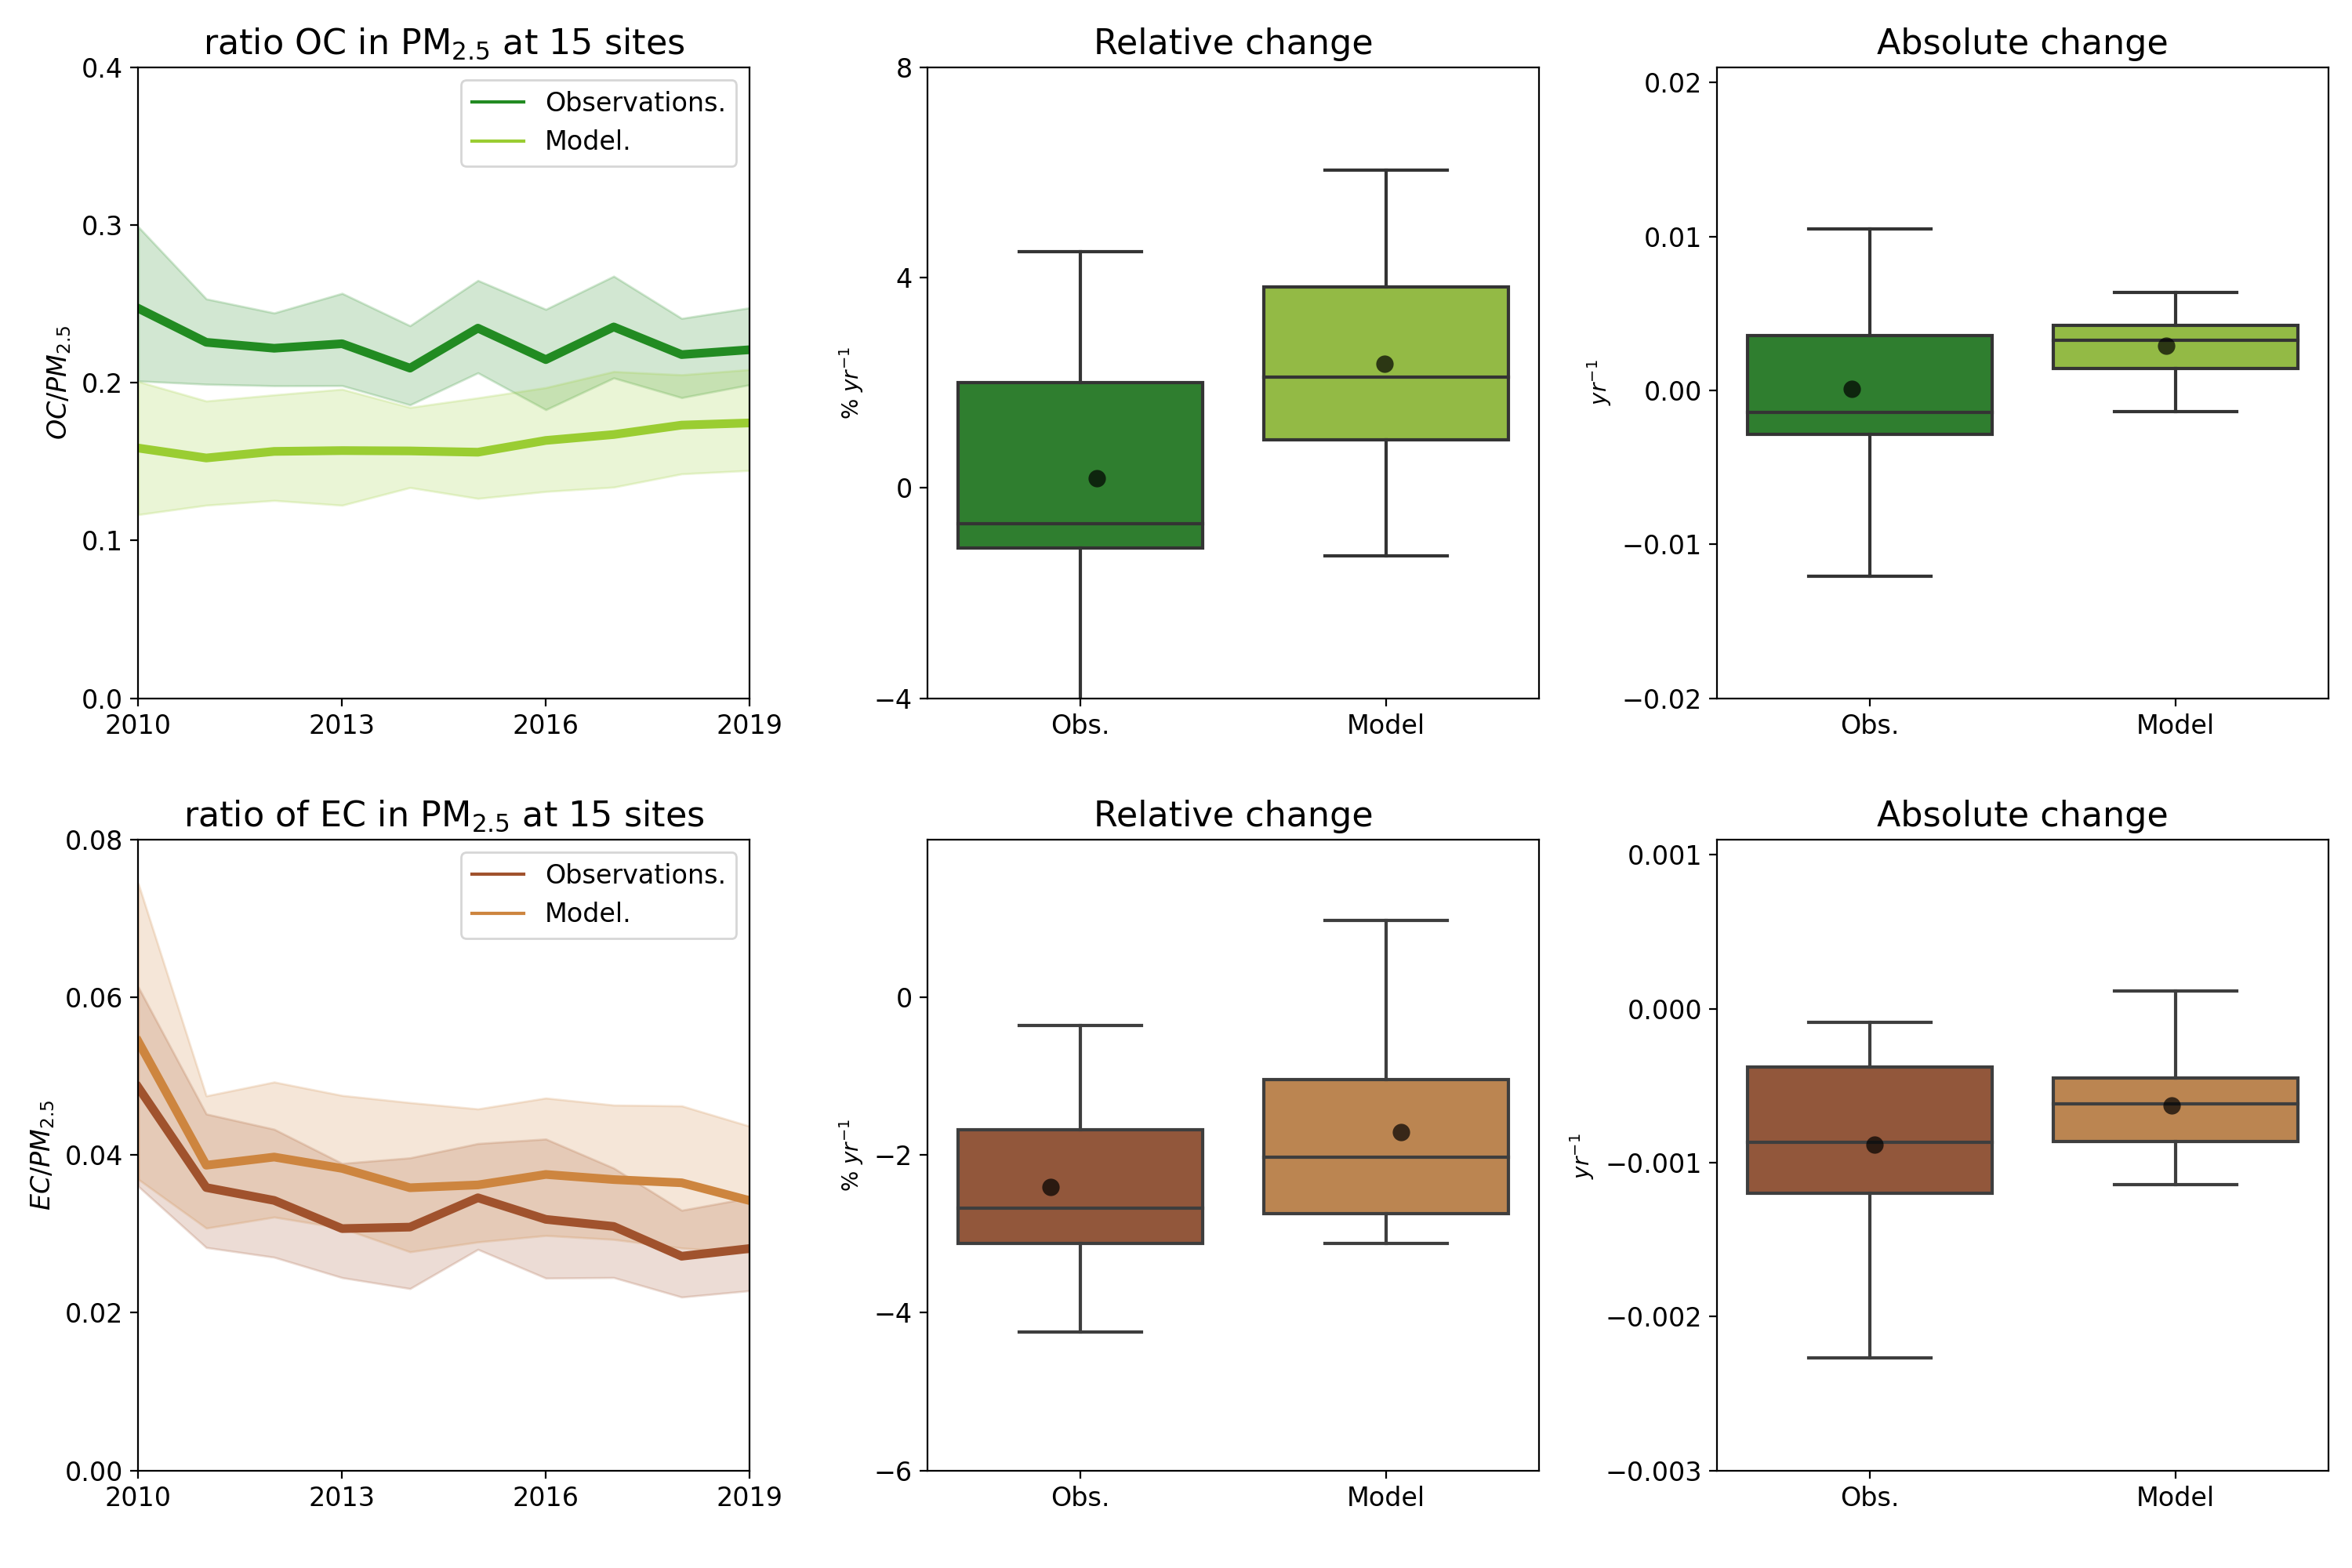
\includegraphics[width=16cm]{FIGS_TRENDS/ECOC_ratio_trends.png}
 \caption{Observed and modeled ratios and trends of OC/\pmfine and EC/\pmfine for
  15 EMEP sites across Europe for 2010--2020, showing the trends
  (left panels) of OC/\pmfine (upper) and EC (lower), aggregated annual and
  seasonal relative changes (mid panels) for OC (upper) and EC (lower),
  and aggregated annual and seasonal absolute changes (right panels)
  for OC (upper) and EC (lower). The solid line in the left panel shows
  the average annual mean for all sites and the shaded area the 95\%
  confidence interval. For explanation of the statistics in the figure,
  see Fig. X.1. \label{fig:KEX3}
 }
\end{figure}

As focused abatement of anthropogenic secondary inorganic aerosol (SIA)
precursors have reduced ambient SIA levels substantially (Sect. \QUERY{X.?}),
other, non-SIA fractions are likely to contribute an increasing fraction
of PM. For the EC fraction of \pmfine, however, there was a -2.4$\pm$1.1\%/yr
reduction for 2010--2020 (Fig.~\ref{fig:KEX3}, Tab.~\ref{tab:KEX3}), showing that EC has been
more efficiently abated than the overall PM mass concentration. The model
calculated a comparable -1.7$\pm$1.3\%/yr reduction for the EC/\pmfine ratio
but predicted a minor increase at two of the sites, which was not seen for
observed EC/\pmfine ratios. For the few sites where measurements allow for
a harmonized data set of EC, OC, \ce{SO4^2-} and \pmfine, i.e., only including
measurements on common days, the reduction in the EC fraction of \pmfine
was typically equally high or higher than for the \ce{SO4^2-} fraction. The
OC fraction of \pmfine showed no decrease or increase (0.2$\pm$2.8\%/yr)
for 2010--2020 when considering all sites, which largely is explained by
non-abatable natural sources making up a major part of OC. A substantial
4.5\%/yr increase in OC/\pmfine was calculated for the Norwegian sites,
experiencing low (anthropogenic) aerosol levels and a high OC fraction
from natural sources, thus one cannot exclude the possibility that part
of this increasing trend is due to an increase in natural sources and
not exclusively from a decrease in anthropogenic emissions. A 2.8\%/yr
increase in the OC fraction was observed for the Spanish site Montseny,
resembling the Norwegian sites with respect to a low aerosol level and
a high OC fraction from natural sources \citep{Kulmala2011}. For the
rest of continental Europe, a minor $\pm$1\%/yr increase/decrease
was seen at most sites and a $\pm$2\%/yr for a few. The Kosetice
(Czech Republic) (-5.3\%/yr) and Shauinsland (Germany) (-3.1\%/yr) sites
experienced a substantial decrease in the OC fraction, which was larger
than the corresponding decrease in the EC fraction, thus deviating from
the pattern seen at all other sites where the decrease in EC/\pmfine $>$
OC/\pmfine.

\begin{figure}
 \caption{
  Mass balance of \pmfine at Ispra (IT04), Birkenes (NO02), Diabla Gora
  (PL05) and Iskrba (SI08) including OM, EC, \ce{SO4^2-}, \ce{NO3^-}, \ce{NH4^+} and mineral
  dust (MD) (IT04 and SI08 only) (left panel) and apportionment of eBC
  into biomass burning/solid fuel (eBCbb) and fossil fuel/liquid fuel
  (eBCff) for winter 2017/2018 (right panel). \label{fig:KEX4}
 }
\end{figure}


The relative contribution of carbonaceous aerosol, OM (OM = OC $\times$
1.4--1.7)
\QUERY{DS: could be $>$2!} and EC, to the \pmfine mass concentration along with the major
SIA species illustrates the importance of the OM fraction for a further
reduction in \pmfine mass concentration (Fig.~\ref{fig:KEX4}). As a first step,
the natural and the anthropogenic fraction of the carbonaceous aerosol
must be separated, then further into abatable categories. Separation of
eBC into biomass burning/solid fuel (eBCbb) and fossil fuel/liquid fuel
(eBCff) is possible using data from the multi wavelength aethalometer,
currently available at $<$25 EMEP/ACTRIS sites across Europe \citep{Platt20XX}
\QUERY{Refs: EMEP, 2020; EMEP, 2019; EMEP, 2014}. An obvious next
step is to implement such analysis as part of regular monitoring,
making it possible to validate not only model performance, but also the
effort made in reducing carbonaceous aerosol from fossil fuel and biomass
burning sources. Although not directly comparable to the multi-year plots
presented in Fig.~\ref{fig:KEX4}, results from the EIMPs Winter 2017/2018 nicely
illustrates the split between eBCbb and eBCff for winter 2017/2018 for
the Italian site Ispra, (IT04), the Norwegian site Birkenes (NO02), the
Polish site Diabla Gora (PL05) and the Slovenian site Iskrba (SI08). The
apportionment of eBC can also be used to infer the corresponding fractions
of OM.

\begin{table}
\centering
\parbox{14cm}{
 \caption{
   Absolute change (\ugC/yr) and relative change (\%/yr) and corresponding
   confidence intervals in observed and modeled annual and seasonal
   aggregated OC/\pmfine and EC/\pmfine ratios at 15 sites across Europe
   for 2010--2020. The number of sites with a significant outcome
   is provided.\label{tab:KEX3}
 }}
 \scalebox{0.95}{%
 \begin{tabular}{lcccccc}
\hline  % toprule
 &  &  &  &  &  &  \\
\multicolumn{7}{c}{EC/\pmfine (2010--2020)} \\
  &  &  &  &  &  &  \\
  \hline
     \multicolumn{3}{c}{Number of sites} & \multicolumn{2}{l}{Average change per year} & \multicolumn{2}{l}{Relative change per year} \\
{} &           total & sign. &                     abs &       Conf. interv. &                      \%/y &   Conf. interv. \\
%How   &                 &       &                         &                     &                          &                 \\
\hline  % midrule
Model &              15 &     5 &                 -0.0006 &  (-0.0009, -0.0004) &                    -1.71 &   (-2.32, -1.1) \\
Obs.  &              15 &     4 &                 -0.0009 &  (-0.0012, -0.0006) &                    -2.41 &  (-2.96, -1.85) \\
\hline  % bottomrule
% \end{tabular}
   &  &  &  &  &  &  \\
\multicolumn{7}{c}{OC/\pmfine (2010--2020)} \\
   &  &  &  &  &  &  \\
% \begin{tabular}{lrrrlrl}
\toprule
   \multicolumn{3}{c}{Number of sites} & \multicolumn{2}{l}{Average change per year} & \multicolumn{2}{l}{Relative change per year} \\
{} &           total & sign. &                     abs &     Conf. interv. &                      \%/y &  Conf. interv. \\
%How   &                 &       &                         &                   &                          &                \\
\hline  % midrule
Model &              15 &     7 &                  0.0029 &   (0.0018, 0.004) &                     2.35 &     (1.3, 3.4) \\
Obs.  &              15 &     2 &                  0.0001 &  (-0.003, 0.0032) &                     0.19 &  (-1.24, 1.62) \\
\hline  % bottomrule
\end{tabular}
} % end scalebox
\end{table}

\subsection{Issues with inventories used in modelling}

\COMMENT{Dave will add text on condensables and EC/OC/remPPM splits - these will affect modelled trends, and add more caveats.}

\subsection{Conclusion}
\label{ss:trendsECOCconc}

A -4.5$\pm$1.6\%/yr reduction in EC was calculated across Europe for
2010--2020 and the reduction was particularly consistent amongst the
sites where the reduction was statistically significant. The model
predicted a reduction that was somewhat lower (-3.9\%/yr) than the
observations, but still comparable. A similar reduction in EC (-4.2\%/yr)
was calculated for 2010--2020 as for 2001--2018 at the Birkenes
Observatory in southern Norway. This consistent reduction indicates a
potential for further reduction in future years for Europe in general,
as LRT from continental Europe explains most EC from both fossil fuel
and biomass burning sources at the Birkenes Observatory. A  -5.2\%/yr
reduction in levoglucosan at the Birkenes Observatory (2010--2020)
 indicate that EC from wood burning in Europe is declining equally
rapid as that of EC from fossil fuel sources.

The reduction in OC (-2.4$\pm$1.6\%/yr) was less pronounced than for EC,
whereas winter-time levels (-4.2\%/yr) were comparable to EC. Non-abatable
natural sources of OC peak in the growing season diluting anthropogenic
sources, thus, anthropogenic OC emissions are likely best represented by
winter-time data. Comparable reductions in winter-time OC (-4.1\%/yr),
winter-time EC (-6.4\%/yr) and winter-time levoglucosan (-4.6\%/yr)
at the Birkenes Observatory suggest that abatement of residential
wood burning emissions has been quite effective for Europe in general,
taking into account considerations about the length of the time series
and Birkenes as an indicator of European emissions.

The model calculated a reduction in OC of -0.6\%/yr, being noticeable
less than for the observations (-2.4\%/yr). A similar underprediction
was seen for each season, thereby reproducing the seasonality in trend
seen for the observations.

The EC fraction of \pmfine (\QUERY{trend }-2.4$\pm$1.1 \%/yr) decreased at all
sites, and at a level equal as, or higher than, the \ce{SO4^2-} fraction. The
change in OC fraction was more scattered with a substantial and
consistent 4.5\%/yr increase at the northernmost sites, whereas
there was no increase or decrease (0.2$\pm$2.8\%/yr) when considering
all sites. Influence of OC from natural sources likely has a profound
impact on the general lack of decrease observed for the OC fraction of
\pmfine. These observations points to a continuous change in the aerosol
chemical composition and in the relative source composition across
Europe. The carbonaceous fraction appears particularly important for a
further reduction in the observed \pmfine mass concentration in Europe,
although effort is needed to separate its natural and anthropogenic
fraction to get a quantitative overview of the abatable fractions.


\clearpage
\bibliographystyle{copernicus}         % change bibliography-name after each
\renewcommand\bibname{References}      % bibliographystyle command!
\addcontentsline{toc}{section}{References}
\bibliography{trends,Refs,EMEP_Reports,NILU,RefsUpdates} % KE, Dave, ...
%\include{chapterTrendsOCandSIA} %Karl-Espen, David

\part{Technical EMEP Developments}
\chapter[Model updates]{Updates to the EMEP MSC-W model, 2020--2021}
\label{ch:ModelUpdates}

%% authors? added all names seen in Log.changes

{\bf{David Simpson, Michael Gauss, Qing Mu, Svetlana Tsyro and Peter Wind}}
\vspace{30pt}

%\old{TODO}
\COMMENT{STARTED Aug 2021. Needs to be filled in by authors}

This chapter summarises the changes made to the EMEP MSC-W  model
since \citet{R2020:ModDev}, and along with changes discussed in
\citet{R2013:ModDev,R2015:ModDev,R2016:ModDev,R2017:ModDev,R2019:ModDev,R2020:ModDev} and
\citet{R2014:ModDev},
updates the standard description given in \citet{Simpson_et_al:EMEP}. The
model version used for reporting this year is denoted rv4.42, which has
had some major updates (especially with regard to emissions) compared to
the rv4.35 reported in \citet{R2020:ModDev}.
Table~\ref{tab:Updates} summarises
the changes made in the EMEP model since the version documented in
\citet{Simpson_et_al:EMEP}, and these changes are discussed in
more detail in Sects.~\ref{sec:updateOverview}-\ref{sec:updateOther}.

%Versions:
%
%  rv4.35 used  for R2020
%  rv4.33 used  for R2019
%  rv4.33 - open source June 2019
%  rv4.32 used for EMEP course, April 2019
%  rv4.17a used for R2018 runs  (July-ish?)
%  rv4.17 released 26/2/2018
%  rv4.16 interim 21/12/2017 - used for N2O5 paper, wheat calculations
%  rv4.15 released 8/9/2017

\section{Overview of changes} 
\label{sec:updateOverview}

%%%%%%%%%%%%%%%%%%%%%%%%%%%%%%%%%%%%%%%%%%%%%%%%%%%%%%%%%%%%%%%%%%%%%%%%%%%%%
\begin{table}
\begin{footnotesize}
\caption{Summary of major EMEP MSC-W model versions from 2012--2020.
Extends Table S1 of \citealt{Simpson_et_al:EMEP}
  COMMENT: Note - recent changes and tags are a little confused. Dave will fix.
}
\label{tab:Updates}
\centering
\begin{tabular}{lp{11cm}l}
\hline
Version & Update                                        & Ref$^{(a)}$   \\
\hline
rv4.42  & Changed default Kz scheme &  This report        \\
        & Updated eissions from CAMS81 project: DMS, soil NO;  &  This report        \\
% 21st May 2021:
rv4.41  & Updated emissions from CAMS81 project: DMS, soil NO; % 16/5
          Modified various params concerning sea-salt and wet-radius calculations; % 16/5
   fracPM25 modified;
          Revised global monthly factor;  % 16/5
        & \\
% 13/5
rv4.40  & Shipping emissions now spread as 20\% below 20m, 80\% between 20-90m;  
          New CAMS81-based aircraft emissions; % 29-30/4
          New CAMS81-based DMS emissions; % 29/4
        & \\
%SKIP BUG fix on aircraft emissions  27/4
% 21/4
rv4.39 &
  GNFR-CAMS is now the default emissions system - see Sect.~\ref{ssec:gnfr};  % 21/4
          Uses global time-zone map;   % 19/3
          Revised global monthly factor?? or rv4.41?;  % 19/3
          New default Kz method introduced (Sect.~\ref{ssec:PBL});
          NWP model rh2m now used in place of earlier sub-grid calculation; % 9/2
          Upgrade of local fractions methodology;  % 7/11/2020
        & \\
% 23/10/2021:
rv4.35  & Various updates, including heavy   
          refactoring of local-fraction code, bug-fixes in MARS module,
          and updates in chemical mechanisms, default PM and NMVOC speciation and
          GenChem systems     & R2020            \\
rv4.34  & Public domain (Feb. 2020); EmChem19a, EmChem19p      & R2020            \\
rv4.33  & Public domain (June 2019);
         EmChem19, PAR bug-fix, EQSAM4clim    & R2019            \\
rv4.32  & Used for EMEP course, April 2019    &    \\
rv4.30  & Moved to new GenChem-based system  &   \\
%        &                                    &        \\
rv4.17a & Used for R2018. Small updates         & R2018      \\
rv4.17  & Public domain (Feb. 2018);
         Corrections in global land-cover/deserts; added
          'LOTOS' option for European \ce{NH3} emissions; corrections
          to snow cover & R2018 \\
rv4.16  & New radiation scheme (Weiss\&Norman); Added dry and wet deposition for \ce{N2O5};
         (Used for  \citealt{Stadtler2018,MillsGCB2018b}) & R2018   \\
rv4.15  & EmChem16 scheme & R2017 \\
%    Sect.\ref{sec:GNFR}--\ref{ss:Splits} & R2016  \\
%
rv4.14  & Updated chemical scheme & R2017       \\
%% rv4.13 + CRI was used in McFiggans. Difficult to describe combo
%        & \\
rv4.12  & New  global land-cover and BVOC & R2017       \\
%        & \\
rv4.10  &  Public domain (Oct. 2016)                 
         (Used for  \citealt{MillsGCB2018a}) &  R2016 \\
%        & \\
rv4.9   & Updates for GNFR sectors, DMS, sea-salt, dust, \ce{S_A} and  $\gamma$, \ce{N2O5} & \\ 
rv4.8   &  Public domain (Oct. 2015); ShipNOx introduced.                          
         Used for EMEP HTAP2 model calculations, see
         special issue:
         \url{www.atmos-chem-phys.net/special_issue390.html},
          and \citet{Jonson_et_al:2017}.              & R2015\\
rv4.7   & Used for reporting, summer 2015;
         New calculations of aerosol surface area; 
         New gas-aerosol uptake and \ce{N2O5} hydrolysis rates; 
         Added 3-D calculations pf aerosol extinction and AODs;
         Emissions - new flexible mechanisms for interpolation and merging sources;
         Global - monthly emissions from ECLIPSE project;
         Global -  LAI changes from LPJ-GUESS model;
         WRF meteorology \citep{SkamarockKlemp2008} can now
     be used directly in EMEP model. & R2015 \\
%        &                                                &\\
rv4.6   & Used for Euro-Delta SOA runs                   & R2015  \\
%QUERY        & Bug-fix for ammonium deposition & \\
       & Revised boundary condition treatments % & \\  % Vertical profiles
       ; ISORROPIA capability added & \\
%       &                                                &\\
rv4.5  & Sixth open-source (Sep 2014);                    
        Improved dust, sea-salt, SOA modelling          % &      \\
       ; AOD and extinction coefficient calculations  updated %& \\
       ; Data assimilation system added % & \\
       ; Hybrid vertical coordinates replace earlier sigma % & \\
       ; Flexibility of grid projection increased. & R2014\\
%SKIP        & ?? Point sources, plume rise, data-assimilation\\
%       &                                                &\\
rv4.4   & Fifth open-source (Sep 2013) %
       ; Improved dust and sea-salt modelling   %          &      \\
       ; AOD and extinction coefficient calculations added %  &\\
       ; gfortran compatibility improved            %      &      \\
                  & R2014, R2013\\
%       &                                                &\\
rv4.3   & Fourth public domain (Mar. 2013)  %
       ; Initial use of namelists           %            & \\
       ; Smoothing of MARS results         %            & \\
       ; Emergency module for volcanic ash and other events% & \\
       ; Dust and road-dust options added as defaults % & \\
       ; Advection algorithm changed  % & \\ % \citet{CLAPP98}    & \\
             & R2013\\ 
%        &                                                &\\
rv4.0   & Third public domain (Sep. 2012), as \citet{Simpson_et_al:EMEP}            & R2013\\ 
%        & As documented in \citet{Simpson_et_al:EMEP}    & \\
%v2011-06& Second public domain (Aug. 2011)                &\\ 
%rv3     & First public domain (Sep. 2008)                &\\ 
        &                                                &\\
\hline
\end{tabular}
Notes: (a) R2018 refers to EMEP Status report 1/2018, etc.
\end{footnotesize}
\end{table}
%%%%%%%%%%%%%%%%%%%%%%%%%%%%%%%%%%%%%%%%%%%%%%%%%%%%%%%%%%%%%%%%%%%%%%%%%%%%%

\begin{itemize}

\item Introduced new soil-NO, DMS and aircraft emissions, from CAMS-81 project
(Sect.~\ref{sec:updateEmis}).  -- Dave, Michael

\item Revised methods for verrtical diffusion (Kz) \QUERY{and Hmix?} (Sect.~\ref{sec:updateKz}). -- Qing

\item Modified fine/coarse split of sea-salt (Sect.~\ref{ssec:updateSS}).  -- Svetlana

\item
Updated Local Fractions calculations (Sect.~\ref{sec:updateLF}). -- Peter

\item  fracPM25 stuff (Sect.~\ref{sec:updateOther}). -- Dave
\item revised wet-radius calculations (Sect.~\ref{sec:updateOther}). --Dave

%\item The EMEP model's chemical pre-processing system and associated box-model (GenChem, boxChem) have been released as open-source.  See Sect.~\ref{sec:GChem}.

\item
Emissions speciation. New default and country-specific emission
speciations for NMVOC and \pmfine have been implemented.  See
Sect.~\ref{ssec:emissplits}.

\item
Numerous small changes to make the code more flexible and/or to
fix minor bugs.

\end{itemize}

In addition to these changes, articles on GenChem (EMEP's chemical pre-processing system)  and
the local-scale extension \COMMENT{Phrasing?} have now been published \citep{Simpson:GenChem,Denby:2020}

%%%%%%%%%%%%%%%%%%%%%%%%%%%%%%%%%%%%%%%%%%%%%%%%%%%%%%%%%%%%%%%%%%%%%%%%%%%%%%
\section{New emission inputs}
\label{sec:updateEmis}

From CAMS81...

\subsection{New basis for emission sectors: GNFR\_CAMS}
\label{ssec:gnfr}

\COMMENT{Text/Table from gmdPaper}
 
Gridded anthropogenic emissions from CEIP
were previously categorized into 11
SNAP sectors, but for many years now EMEP emission reporting has been conducted and prepared for
modelling using the 13-sector
GNFR system\footnote{
GNFR=Gridding nomenclature for reporting/UNECE nomenclature for reporting of emissions to air,
e.g. \citealt{CEIP2020:GNFR}}.
In 2020 a 19-sector emission system (`GNFR\_CAMS') was implemented in the EMEP model, to take care of
emissions provided by TNO as part of the Copernicus CAMS project \citep{Kuenen2021}. This extended emissions system
enables for example four road traffic sectors, F1--F4, with e.g. F1
 representing exhaust emissions from gasoline vehicles.
Such emission sectors are characterised in the model by
release heights, timefactors and species-splits (e.g. NOx to NO and
\ce{NO2}, or NMVOC to individual VOC surrogates) for each sector.

Table~\ref{tab:GNFRsectors} summarises the new GNFR\_CAMS sectors,
and the mapping indices used.
%\COMMENT{Add index explanation in SI table?}


\begin{table}
\caption{The `GNFR\_CAMS' 19-sector system, and mapping indices for release heights, timefactors and species-splits,
 which is now
 default in EMEP model. \label{tab:GNFRsectors}
}
\begin{tabular}{lrrrrlc}
\hline
code & Number  & \multicolumn{3}{c}{Index}      & sector & SNAP \\ \cline{3-5}
     &         & timefac  & height & emissplit  &        & equivalent \\
\hline
A &      01 &   1 &  1 &   1 &  Public Power  &  1 \\
B &      02 &   3 &  3 &   2 &  Industry  & 3, 4 \\
C &      03 &   2 &  2 &   3 &  Other Stationary Combustion & 2 \\
D &      04 &   4 &  4 &   4 &  Fugitive & ??  \\
E &      05 &   6 &  2 &   5 &  Solvents & 6 \\
F &      06 &   7 &  2 &   6 &  Road Transport & 7 \\
G &      07 &   8 &  2 &   7 &  Shipping & 8  \\
H &      08 &   8 &  7 &   8 &  Aviation & 8  \\
I &      09 &   8 &  2 &   9 &  Offroad & 8  \\
J &     10 &   9 &  6 &  10 &  Waste & ? \\
K &     11 &  10 &  2 &  11 &  Agri - Livestock & 10 \\
L &     12 &  10 &  2 &  12 &  Agri - Other & 10 \\
M &     13 &   5 &  5 &  13 &  Other & 11 \\
A1 &    14 &   1 &  1 &   1 &  PublicPower - Point & 1 \\
A2 &    15 &   1 &  3 &   1 &  PublicPower - Area & 1 \\
F1 &    16 &   7 &  2 &  16 &  Road Transport - Exhaust Gasoline & 7  \\
F2 &    17 &   7 &  2 &  17 &  Road Transport - Exhaust Diesel& 7   \\
F3 &    18 &   7 &  2 &  18 &  Road Transport - Exhaust LPGgas & 7  \\
F4 &    19 &   7 &  2 &  19 &  Road Transport - NonExhaust Other& 7   \\
\hline
\end{tabular}
\end{table}



\subsection{Soil NO emissions}
\label{ssec:soilNO}

\COMMENT{DAVE to COMPLETE}

\subsection{DMS emissions}
\label{ssec:DMS}

\COMMENT{MICHAEL to COMPLETE}

\subsection{Aircraft emissions}
\label{ssec:Aircraft}

\COMMENT{MICHAEL to COMPLETE}


\subsection{Revised fine/coarse splits of sea-salt emissions}
\label{ssec:updateSS}

\COMMENT{SVETLANA to COMPLETE}



%%%%%%%%%%%%%%%%%%%%%%%%%%%%%%%%%%%%%%%%%%%%%%%%%%%%%%%%%%%%%%%%%%%%%%%%%%%%%%
\subsection{Emission speciation}
\label{ssec:emissplits}.

\COMMENT{OLD:}

The emissions speciation of NMVOC and primary PM (PPM) were updated
for the EmChem19a scheme to reflect recent data available from
the latest TNO/CAMS inventories (see chap.~\ref{chap:TNO} 
\COMMENT{Dave will sort out cross-refs}
, also
\citealt{CAMSemis2019}).  For NMVOC the main changes have been:

\begin{enumerate}
  \item Use TNO NMVOC speciation

    TNO provided NMVOC speciation data for 25 compounds from each
    GNFR\_CAMS category, as part of the CAMS-REG-v3.1.2 database,
    which were then mapped to the EmChem19a species.

  \item Improve country-specific road transport estimates

    TNO provided country-specific fractions of the four road-traffic
    sectors in the CAMS-REG-AP\_v2.2.1 inventory for 2015, specifically
    F1=gasoline exhaust, F2=diesel exchaust, F3=LPG exhaust, and
    F4=non-exhaust emissions. These were also aggregated to form
    country-specific NMVOC splits for the generic GNFR F category
    (road transport).

\end{enumerate}

% PM TNO CAMS-REG_AP_v2.2.1_2015_REF

For \pmfine and \pmten, we made use of country-data generated by TNO for
the TFMM Euro-DeltaCarb simulations, which gave EC, OM (named
OC in the files), Na, SO4 and other compounds, as well as the fraction
of modern carbon in the GNFR-C categories. These data were aggregated
to the EMEP models EC, OM, and remPPM compounds. Data were provided for
both the Ref1 and Ref2 cases (see Chap.~\ref{chap:TNO}), and we assume
that Ref1 data are appropriate for modelling with officially submitted
emissions, and Ref2 data appropriate for modelling when Ref2 emissions
are used (e.g. for the \textbf{EMEPwRef2C} simulations discussed in
Chapters~\ref{ch:chapterStatus}--\ref{ch:Condensables}).
\COMMENT{Dave will sort out text later}



%%%%%%%%%%%%%%%%%%%%%%%%%%%%%%%%%%%%%%%%%%%%%%%%%%%%%%%%%%%%%%%%%%%%%%%%%%%%%%
\section{Revised PBL paramterisations}
\label{sec:updateKz}

\COMMENT{QING to UPDATE}

%%%%%%%%%%%%%%%%%%%%%%%%%%%%%%%%%%%%%%%%%%%%%%%%%%%%%%%%%%%%%%%%%%%%%%%%%%%%%%
\section{Local Fractions}
\label{sec:updateLF}

\COMMENT{PETER to UPDATE}

%%%%%%%%%%%%%%%%%%%%%%%%%%%%%%%%%%%%%%%%%%%%%%%%%%%%%%%%%%%%%%%%%%%%%%%%%%%%%%
\section{Other?}
\label{sec:updateOther}

fracMPM25 - Dave
revised wet-radius calculations --Dave

Something on pollen perhaps? -- Alvaro??



\clearpage
\bibliographystyle{copernicus}         % change bibliography-name after each
\renewcommand\bibname{References}      % bibliographystyle command!
\addcontentsline{toc}{section}{References}
\bibliography{Refs,EMEP_Reports,uEMEP}

\chapter[Development of measurements]{Developments in the monitoring network, data quality and database infrastructure}\label{ch:ObsDevel}
%DS changed to Ch~X.X notation

{\bf{Wenche Aas, Anne Hjellbrekke and Kjetil T{\o}rseth}}
\vspace{30pt}

\section{\label{sec:Compliance-with-monitoring}Compliance with the EMEP monitoring strategy}

The monitoring obligations of EMEP were updated in 2019 and is defined by the Monitoring Strategy for 2020-2030 (\cite{MonStrat2019}). 

The complexity in the monitoring program with respect to the number of variables and sites, whether parameters are at level 1 or level 2, and the required time resolution (hourly, daily, weekly), makes it challenging to assess whether a country is in compliance. CCC has developed an index to illustrate to what extent the Parties comply, how implementation compares with other countries, and how activities evolve with time.

The index is defined for level 1 parameters only, and is calculated based on the data reported in comparison with the expected. EMEP recommends one site pr 50.000 km$^{2}$, but this target number is adjusted for very large countries (i.e. KZ, RU, TR and UA). The components and number of variables to be measured in accordance to the strategy are as follows: major inorganic ions in precipitation (10 variables), major inorganic components in air (13 variables), ozone (1 variable), PM mass (2 variables) and heavy metals in precipitation (7 variables). For heavy metals, the sampling frequency is weekly, and for the other components it is daily or hourly (ozone). Based on the relative implementation of the different variables, the index has been given the following relative weights: Inorganics in precipitation: 30\%, inorganics in air: 30\%, ozone: 20\%, PM mass: 10\%, heavy metals: 10\%.

Figure~\ref{fig:Index-for-implementation} summarises implementation in 2019 compared to 2000, 2005 and 2010. The countries are sorted from left to right with increasing index for 2019. Slovakia,  Estonia, The Netherlands, Denmark, and Switzerland have almost complete programs with an index of 90\% or higher. Small countries generally comply better (due to more easily satisfying the site density requirements). Since 2010, 35\% of the Parties have improved their monitoring programme,  while 37\% have a decrease. Improvements are seen in e.g. France, Croatia and Belgium.  One Party, Malta, has reported data in 2019 and not in 2010, while Georgia, Moldova, Montenegro and Romania have stopped reporting/measuring. In Figure~\ref{fig:EMEP-measurement-network} in Ch~\ref{Obs_2019}, the geographical distribution of level 1 sites is shown for 2019.  In large parts of Europe, implementation of the EMEP monitoring strategy is far from satisfactory. 

\begin{figure}
	\centering
	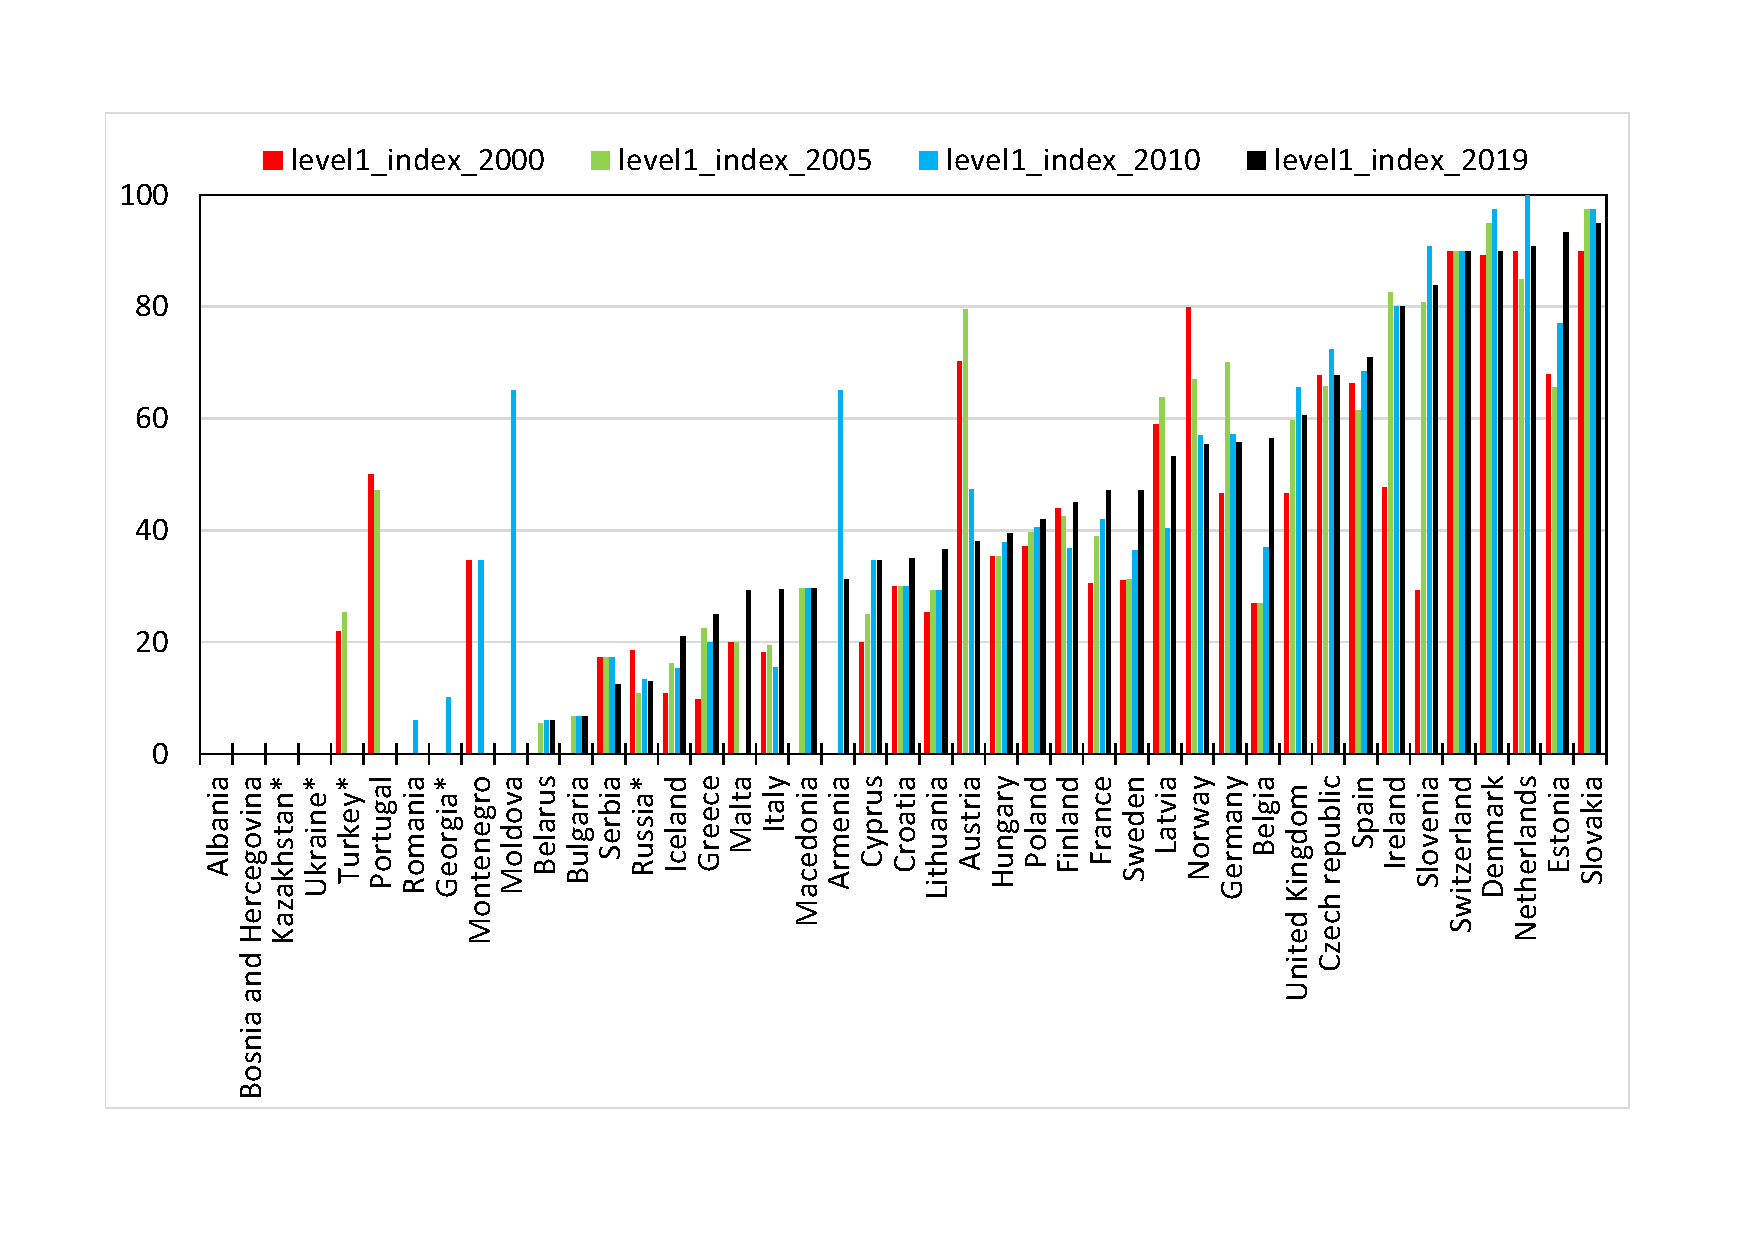
\includegraphics[width=0.74\paperwidth]{FIGS_Obs/index2019.pdf}
	\caption{\label{fig:Index-for-implementation}Index for implementation of the EMEP monitoring strategy, level 1 based on what has been reported for 2000, 2005, 2010 and 2019. {*} means adjusted land area.}
\end{figure}

For the level 2 parameters, an index has not been defined, but mapping the site distribution illustrate the compliance to the monitoring strategy. 56 sites from 21 different Parties reported  at least one of the required  EMEP level 2 parameters relevant to this report (aerosols (50 sites), photo-oxidants (16 sites) and atmospheric tracers (8 sites)). One should note that some of these sites have been reporting data to ACTRIS (the European Research Infrastructure for the observation of Aerosol, Clouds and Trace Gases) and not to EMEP, but they have been included here in the overview since the observations are still comparable with those of EMEP. The sites with measurements of POPs and heavy metals are covered in the EMEP status report published by MSC-E (EMEP Status report 2/2021).  Figure~\ref{fig:levell2-sites} shows that level 2 measurements of aerosols have better spatial coverage than oxidant precursors (VOC + methane) and atmospheric tracers. Few sites have a complete measurement program, the aerosol program is most developed with 12 sites having a complete aerosol program. For oxidant precursors and atmospheric tracers, there are ongoing improvement in the measurement capabilities resulting from development in ACTRIS in co-operation with EMEP and the WMO Global Atmospheric Watch Programme (GAW).

\begin{figure}[h!]
 \centering
  \subfigure[Particulate matter] {\includegraphics*[width=0.3\linewidth]{FIGS_Obs/pm_level_2.png}}
  \subfigure[Oxidant precursors] {\includegraphics*[width=0.3\linewidth]{FIGS_Obs/oxidants.png}}
  \subfigure[Atmospheric tracers] {\includegraphics*[width=0.3\linewidth]{FIGS_Obs/tracer.png}}
\caption{\label{fig:levell2-sites}Sites measuring and reporting EMEP level 2 parameters for the year 2019.}
\end{figure}

\section{Updates in reporting templates and guidelines}

In addition to the requirement that variables has to be measured as defined in the EMEP monitoring 
strategy discussed above, it is important that the data are reported in time to ensure that they can 
be quality assured and included in the database. This allows them to be included in the annual model 
validation, interpretations for the EMEP status reports, as well as other regional assessments and 
studies carried out beyond EMEP.

Figure~\ref{fig:Submission} shows the status of the submission of data for 2019  and to what  extent the data were reported in time. It is obvious that large volumes of data are reported late and some not at all. Of the 33 Parties reporting either level 1 or level 2 data, about  60\% reported within the deadline of 31 July 2020. 

\begin{figure}[h]
\centering
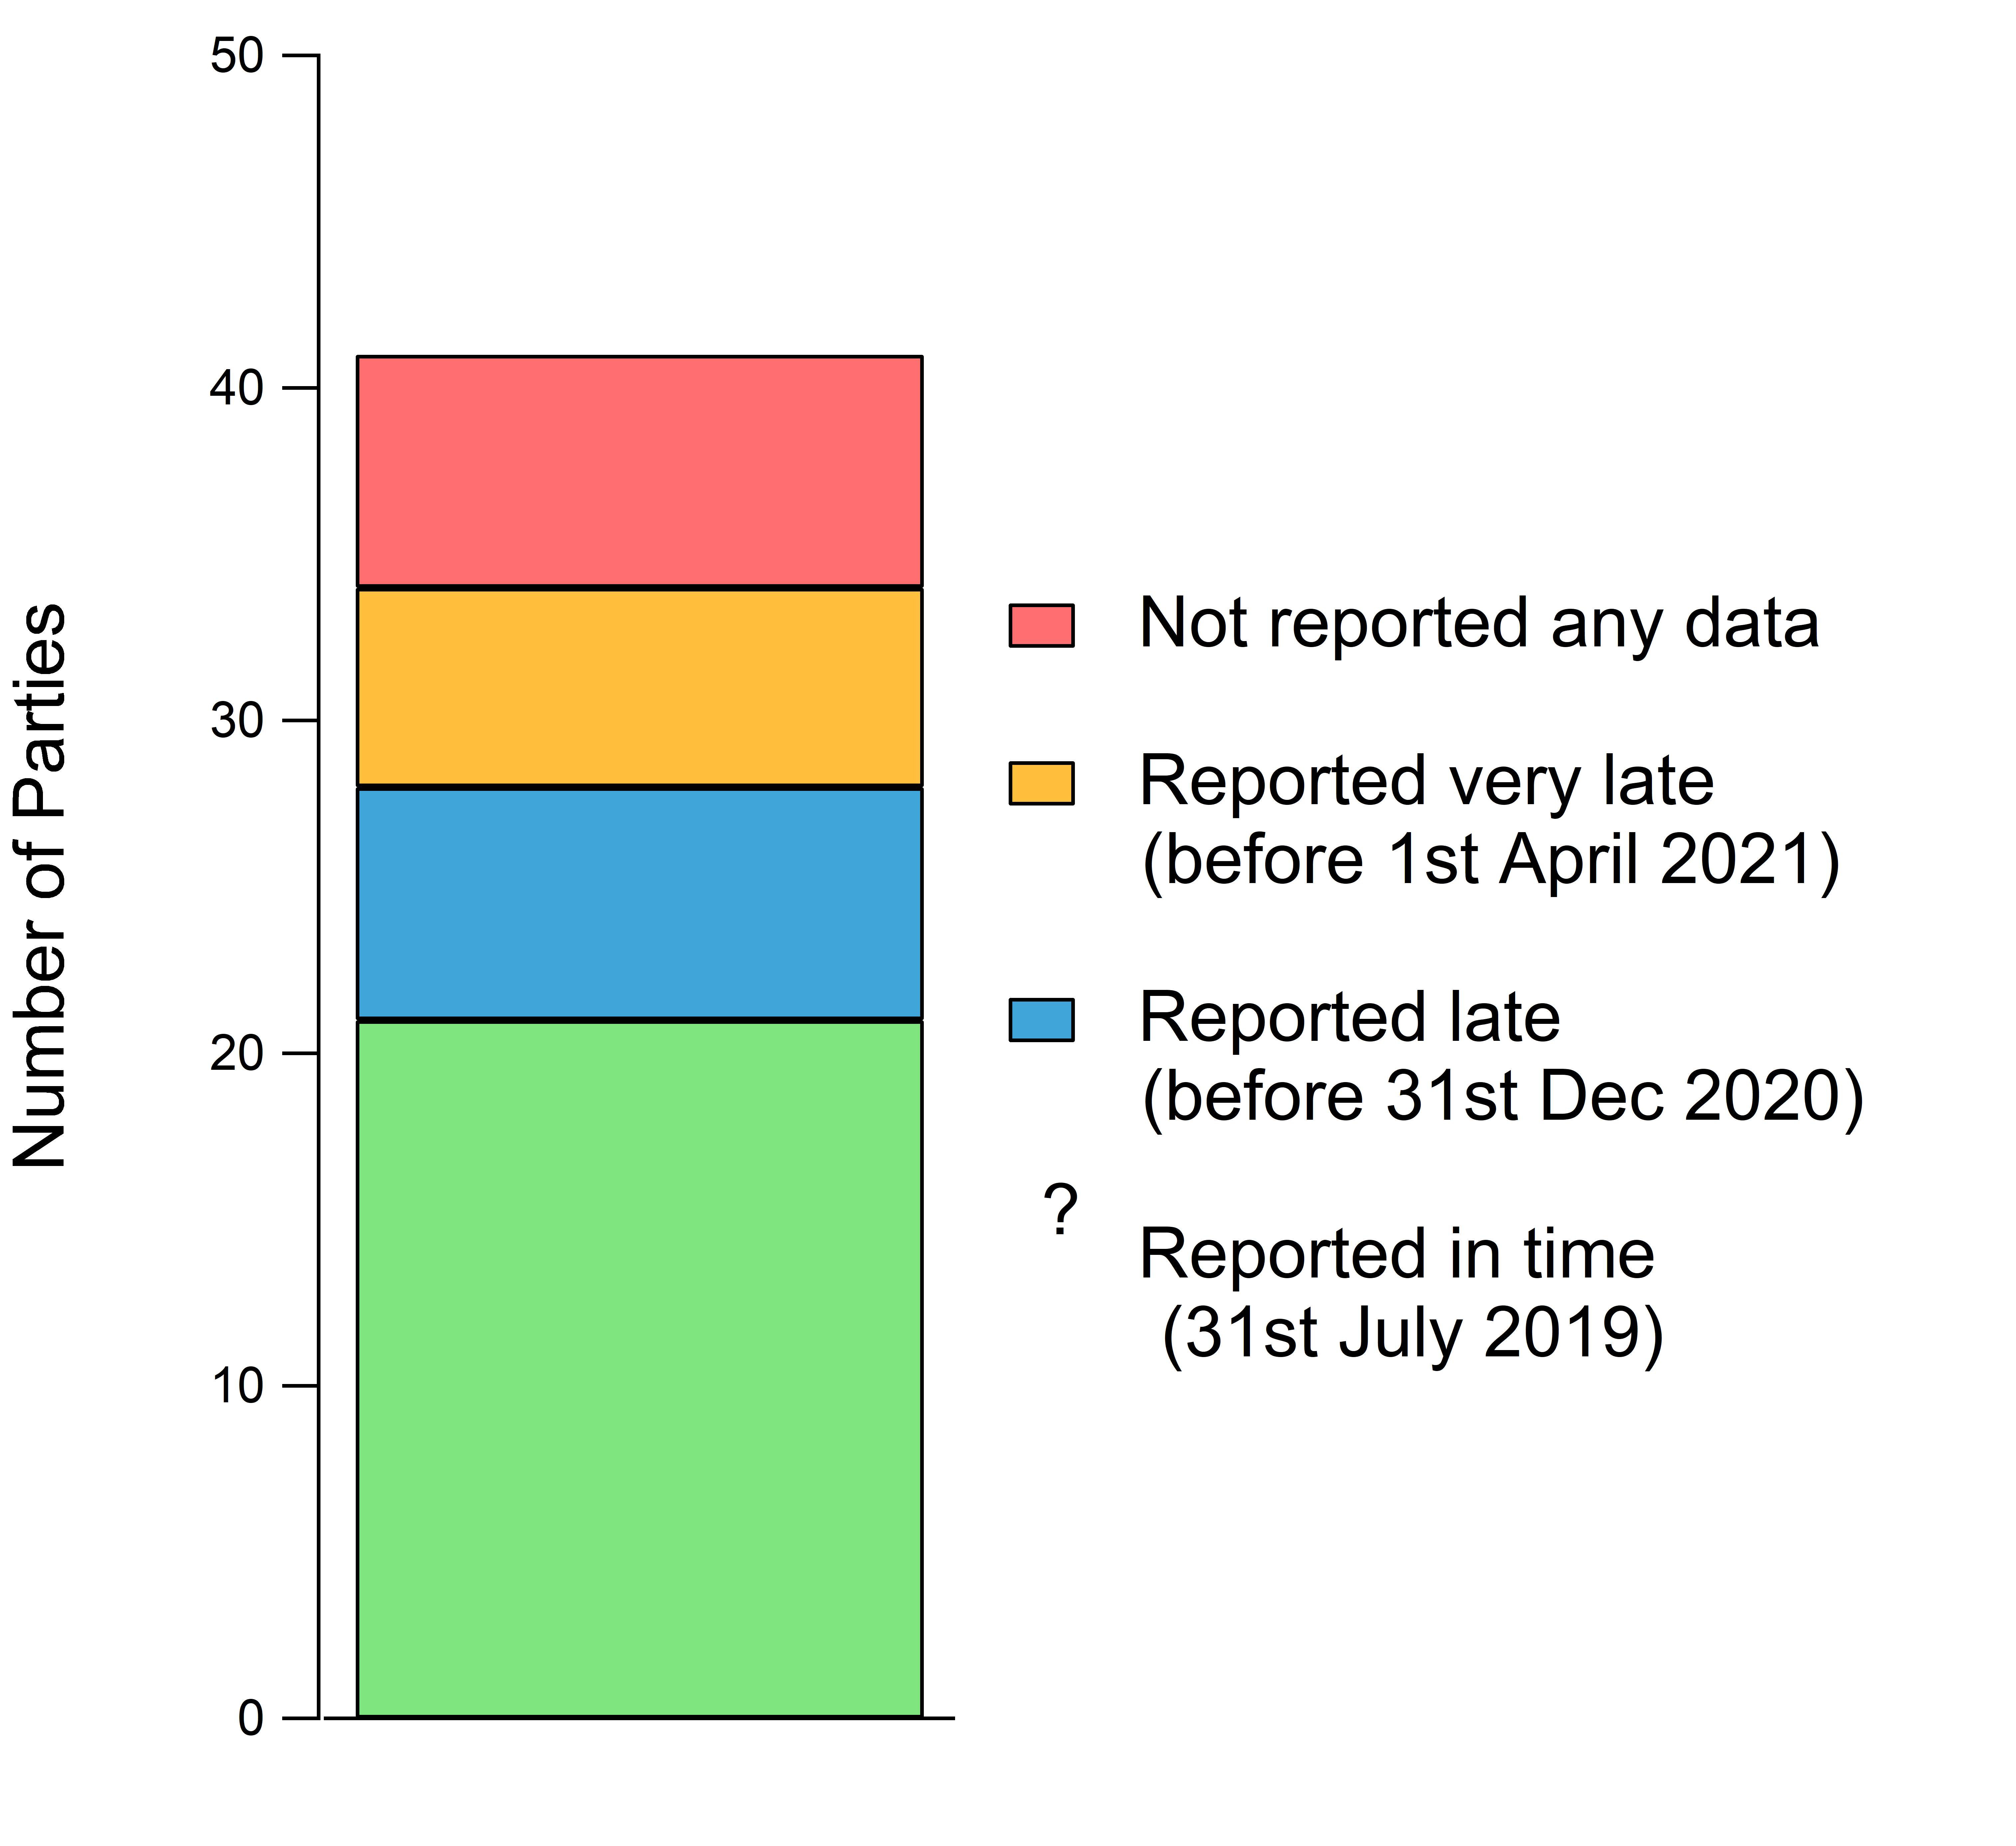
\includegraphics[width=0.45\paperwidth]{FIGS_Obs/reported.png}
\caption{\label{fig:Submission}Submission of 2019 data to EMEP/CCC.}
 \end{figure}

An online data submission and validation tool (\url{http://ebas-submit-tool.nilu.no}) was developed in 2016 improve  the timeliness and quality of the data reporting. The tool is designed to give the data submitters direct feedback on the formatted NASA Ames files, and suggestions on how to correct the files.  The format checker is directly linked to all (approx. 40) data format templates located at \url{http://ebas-submit.nilu.no/}, and it  is continuously being improved and updated, after feedback from the users or when new templates are developed. 

The requirement of checking the data files using the submission tool has significantly improved the correctness in the data files submitted, but still there are Parties not using the submission tool and report by e-mails. EMEP/CCC strongly encourage all the Parties to use the submission tool, which in fact is mandatory for submitting all the data to EMEP, unless otherwise have been agreed upon. In the coming years there will be further focus on improving the data submission tools to make it easier for the data provider to report correct and consistent data. 

The EMEP data are extensively used. In 2009, a user statistic was implemented for the EBAS database infrastructure.  
The statistic counts how much data are downloaded, displayed or plotted. Figure~\ref{fig:downloads} shows the access requests for EMEP data per year (about 300 thousand annual datasets). There was a big jump in 2013. This was the year when an automatic system for distributing all the data in EBAS to specific users was implemented. The number of downloads increased somewhat in 2020 compared to 2019. 

\begin{figure}[h]
\centering
\includegraphics[width=0.6\paperwidth]{FIGS_Obs/downloaded.png}
\caption{\label{fig:downloads}Access of EMEP data, number of annual dataset (compounds) per year.}
 \end{figure}

There is ongoing work to make the  access of data even more flexible to meet several of the user needs. In example using other platforms, like THREDDS (\url{https://thredds.nilu.no/thredds/catalog/ebas/catalog.html}) where NetCDF files are extracted from EBAS allowing faster access and the possibility to create more individual specific defined outputs for plotting, statistics, aggregates etc.: Further, a system for issuing Persistent Identifiers of datasets (Digital Object Identifiers – DOIs) is currently under development/implementation. The development of the database infrastructure is scoped to comply with the FAIR principles (findable, accessible, interoperable and reusable).

\clearpage
\bibliographystyle{copernicus}         % change bibliography-name after each
\renewcommand\bibname{References}      % bibliographystyle command!
\addcontentsline{toc}{section}{References}
%\bibliography{Refs,EMEP_Reports}
\bibliography{Refs2021}


\part{Appendices}
\setcounter{part}{1}
\cleardoublepage
\setcounter{page}{1}
\begin{appendix}
\renewcommand{\theHchapter}{\Alph{chapter}}
\renewcommand{\thepage}{{\em page \Alph{chapter}:\arabic{page}}}
\renewcommand{\thepage}{{\Alph{chapter}:\arabic{page}}}
\renewcommand{\thetable}{\Alph{chapter}:\arabic{table}}

% do this here for safety!!!
\setcounter{page}{1}

%Leave this here in order to start the whole on an odd-numbered page
\cleardoublepage
\chapter[2019 Emissions]{National emissions for 2019 in the EMEP domain}
\label{ch:appx_emis_2019}


This appendix contains the national emission data for 2019 used throughout this
report for main pollutants and  primary particle emissions in the new 
EMEP domain, which covers the geographic area between 30\degrees N-82\degrees N latitude and 30\degrees W-90\degrees E longitude. \\

These are the emissions that are used as basis
 for the 2019 source-receptor calculations. Results of these
 source-receptor calculations are presented in Appendix~\ref{ch:appx_sr2019}.\\

The land-based emissions for 2019 have been derived from the 2021
official data submissions to UNECE CLRTAP \old{Update reference later \citep{CEIP2021}}.


This year two different estimates for primary PM emissions have been available for the modeling: 1) EMEP emissions as prepared by CEIP based on the official data submissions for 2019, and 2) EMEP PM emissions where condensable organics from small-scale combustion are accounted for by using expert emission estimates for GNFR sector C from the TNO REF2.1 data set for the following countries: Albania, Austria, Bosnia and Herzegovina, Belarus, Switzerland, Cyprus, Germany, Estonia, France,  Ireland, Lithuania, Montenegro, Poland, Russian Federation, Slovakia, Turkey and Ukraine.
  %For more details please consult Chapter~\ref{ch:Condensables}.
In this report 1) is referred to as EMEP and 2) is referred to as EMEPwREF2.1C. National emission totals for both data sets are shown in Table~\ref{tab:2019emisPM}.  \\

Emissions from international shipping occurring in different European seas within the EMEP domain are not reported to UNECE CLRTAP, but derived from other sources. This year's update uses the CAMS global shipping emissions \old{New reference? \citep{CAMSemis2019}}  developed by FMI (Finnish Meteorological Institute).
\\

Natural marine emissions of dimethyl sulphid (DMS) are calculated dynamically during the model run and vary with current meteorological conditions.\\

\sox emissions from passive degassing of Italian volcanoes (Etna, Stromboli and Vulcano) are reported by Italy. \\

Note that emissions in this appendix are given in different units than used elsewhere in this report in order to keep consistency with the reported data.


\clearpage

\bibliographystyle{copernicus}
\renewcommand\bibname{References}    
\addcontentsline{toc}{section}{References}
\bibliography{Refs,EMEP_Reports}

\clearpage
 
\begin{table}
\caption{National total emissions of main pollutants for 2019 in the EMEP
  domain. Unit: Gg. (Emissions of SO$_x$ and NO$_x$ are given as
  Gg(SO$_2$) and Gg(NO$_2$), respectively.)}
\label{tab:2019emisMAIN}

\vspace{15pt}

\begin{center}
\scriptsize
\begin{tabular}{|l|r|r|r|r|r|}
\hline
 Area/Pollutant&SO$_x$&NO$_x$&NH$_3$&NMVOC&CO\\\hline\hline
                       Albania&     6&    28&    20&    34&    77 \\\hline
                       Armenia&     6&    42&    15&    26&    76 \\\hline
                       Austria&    11&   144&    64&   109&   498 \\\hline
                    Azerbaijan&    79&   294&    79&   378&   665 \\\hline
                       Belarus&    45&   128&   134&   276&   696 \\\hline
                       Belgium&    30&   160&    66&   113&   369 \\\hline
        Bosnia and Herzegovina&    93&    51&    22&   100&   242 \\\hline
                      Bulgaria&    88&    97&    44&    72&   254 \\\hline
                       Croatia&     8&    54&    37&    75&   216 \\\hline
                        Cyprus&    16&    14&     7&     9&    11 \\\hline
                       Czechia&    80&   172&    85&   215&   819 \\\hline
                       Denmark&    10&    99&    75&   103&   209 \\\hline
                       Estonia&    19&    25&    11&    23&   131 \\\hline
                       Finland&    29&   120&    32&    85&   345 \\\hline
                        France&   100&   774&   593&   956&  2375 \\\hline
                       Georgia&    21&    47&    33&    31&   109 \\\hline
                       Germany&   264&  1137&   587&  1121&  2883 \\\hline
                        Greece&    80&   250&    64&   144&   464 \\\hline
                       Hungary&    17&   114&    79&   119&   354 \\\hline
                       Iceland&    58&    21&     5&     5&   106 \\\hline
                       Ireland&    11&   101&   125&   114&    68 \\\hline
                         Italy&   105&   627&   355&   894&  2062 \\\hline
                    Kazakhstan&  2210&   869&   109&   595&  1458 \\\hline
                    Kyrgyzstan&    39&    62&    32&    42&   206 \\\hline
                        Latvia&     4&    33&    18&    41&   120 \\\hline
                 Liechtenstein&     0&     0&     0&     0&     0 \\\hline
                     Lithuania&    12&    52&    35&    52&   116 \\\hline
                    Luxembourg&     1&    19&     6&    11&    21 \\\hline
                         Malta&     0&     5&     1&     3&     7 \\\hline
                       Moldova&     7&    41&    20&    77&   174 \\\hline
                        Monaco&     0&     0&     0&     0&     2 \\\hline
                    Montenegro&    25&    13&     4&     9&    34 \\\hline
                   Netherlands&    23&   238&   123&   237&   626 \\\hline
               North Macedonia&   116&    21&     8&    24&    55 \\\hline
                        Norway&    16&   151&    29&   153&   400 \\\hline
                        Poland&   427&   682&   317&   647&  2112 \\\hline
                      Portugal&    44&   148&    59&   161&   293 \\\hline
                       Romania&    99&   217&   178&   230&   894 \\\hline
            Russian Federation&  1368&  3133&  1219&  3838& 12373 \\\hline
                        Serbia&   395&   129&    76&   121&   330 \\\hline
                      Slovakia&    16&    61&    31&   100&   279 \\\hline
                      Slovenia&     4&    29&    18&    31&    97 \\\hline
                         Spain&   149&   646&   471&   608&  1600 \\\hline
                        Sweden&    16&   127&    53&   134&   336 \\\hline
                   Switzerland&     4&    61&    54&    81&   161 \\\hline
                    Tajikistan&    42&    49&    34&    86&   526 \\\hline
                        Turkey&  2455&   862&   765&  1121&  1674 \\\hline
                  Turkmenistan&   113&   265&    73&   187&   903 \\\hline
                       Ukraine&   508&   614&   246&   384&  2835 \\\hline
                United Kingdom&   163&   843&   272&   813&  1585 \\\hline
                    Uzbekistan&   325&   346&   200&   317&  1174 \\\hline
                   Asian areas&  5289&  6651&  3301&  9368& 33748 \\\hline
                  North Africa&  1230&  1266&   408&  1602&  3241 \\\hline
                    Baltic Sea&    11&   349&     0&     3&    28 \\\hline
                     Black Sea&    50&   112&     0&     1&    10 \\\hline
             Mediterranean Sea&   750&  1519&     0&    13&   120 \\\hline
                     North Sea&    36&   758&     0&     7&    67 \\\hline
     North-East Atlantic Ocean&   494&   931&     0&     8&    75 \\\hline
      Natural marine emissions&  2926&     0&     0&     0&     0 \\\hline
            Volcanic emissions&   943&     0&     0&     0&     0 \\\hline\hline
                         TOTAL& 21486& 25803& 10691& 26105& 80709 \\\hline

\end{tabular}
\end{center}
\end{table}


\clearpage
 
\begin{table}
\caption{National total emissions of particulate matter for 2019 in the EMEP
  domain. Unit: Gg. }
\label{tab:2019emisPM}

\vspace{15pt}

\begin{center}
\scriptsize
\begin{tabular}{|l|r|r|r|r||r|r|r|}
\hline
 Area/Pollutant& BC&PM$_{2.5}$&PM$_{co}$&PM$_{10}$&PM$_{2.5}$&PM$_{co}$&PM$_{10}$\\
 &&EMEP&EMEP&EMEP&EMEPwREF2.1C&EMEPwREF2.1C&EMEPwREF2.1C\\\hline\hline
                       Albania&     2&    13&     3&    15&    12&     2&    14 \\\hline
                       Armenia&     1&     8&     2&    10&     8&     2&    10 \\\hline
                       Austria&     4&    14&    12&    26&    34&    12&    46 \\\hline
                    Azerbaijan&     9&    38&    10&    48&    38&    10&    48 \\\hline
                       Belarus&     8&    56&    18&    73&    55&    17&    72 \\\hline
                       Belgium&     3&    18&     9&    27&    18&     9&    27 \\\hline
        Bosnia and Herzegovina&     6&    46&    10&    56&    36&     9&    46 \\\hline
                      Bulgaria&     4&    30&    17&    46&    30&    17&    46 \\\hline
                       Croatia&     4&    29&    12&    41&    29&    12&    41 \\\hline
                        Cyprus&     0&     1&     1&     2&     1&     1&     2 \\\hline
                       Czechia&     5&    36&    11&    47&    36&    11&    47 \\\hline
                       Denmark&     2&    13&    10&    23&    13&    10&    23 \\\hline
                       Estonia&     2&     6&     3&     9&    15&     4&    19 \\\hline
                       Finland&     4&    17&    13&    30&    17&    13&    30 \\\hline
                        France&    21&   121&    81&   202&   183&    84&   266 \\\hline
                       Georgia&     6&    24&     4&    28&    24&     4&    28 \\\hline
                       Germany&    12&    92&   112&   204&   122&   111&   233 \\\hline
                        Greece&     9&    37&    24&    61&    37&    24&    61 \\\hline
                       Hungary&     6&    40&    22&    62&    40&    22&    62 \\\hline
                       Iceland&     0&     1&     1&     2&     1&     1&     2 \\\hline
                       Ireland&     2&    12&    16&    28&    10&    16&    26 \\\hline
                         Italy&    18&   139&    33&   172&   139&    33&   172 \\\hline
                    Kazakhstan&    17&   137&    71&   208&   137&    71&   208 \\\hline
                    Kyrgyzstan&     1&    14&     5&    19&    14&     5&    19 \\\hline
                        Latvia&     3&    20&     9&    29&    20&     9&    29 \\\hline
                 Liechtenstein&     0&     0&     0&     0&     0&     0&     0 \\\hline
                     Lithuania&     1&     5&     6&    11&    21&     6&    27 \\\hline
                    Luxembourg&     0&     1&     1&     2&     1&     1&     2 \\\hline
                         Malta&     0&     0&     1&     1&     0&     1&     1 \\\hline
                       Moldova&     3&    27&     5&    32&    27&     5&    32 \\\hline
                        Monaco&     0&     0&     0&     0&     0&     0&     0 \\\hline
                    Montenegro&     1&     7&     1&     9&     5&     1&     6 \\\hline
                   Netherlands&     2&    15&    12&    28&    15&    12&    28 \\\hline
               North Macedonia&     1&     8&     5&    13&     8&     5&    13 \\\hline
                        Norway&     3&    24&     9&    32&    24&     9&    32 \\\hline
                        Poland&    14&   122&    97&   218&   251&    70&   321 \\\hline
                      Portugal&     7&    50&    20&    71&    50&    20&    71 \\\hline
                       Romania&    13&   112&    41&   153&   112&    41&   153 \\\hline
            Russian Federation&    46&   303&   425&   729&   659&   436&  1096 \\\hline
                        Serbia&     6&    46&    16&    61&    46&    16&    61 \\\hline
                      Slovakia&     2&    18&     5&    23&    19&     6&    25 \\\hline
                      Slovenia&     2&    11&     3&    13&    11&     3&    13 \\\hline
                         Spain&    29&   135&    60&   195&   135&    60&   195 \\\hline
                        Sweden&     2&    18&    19&    37&    18&    19&    37 \\\hline
                   Switzerland&     1&     6&     8&    14&    12&     8&    20 \\\hline
                    Tajikistan&     5&    30&     9&    40&    30&     9&    40 \\\hline
                        Turkey&    32&   384&   169&   553&   413&   141&   554 \\\hline
                  Turkmenistan&     4&    26&     8&    34&    26&     8&    34 \\\hline
                       Ukraine&    25&   281&   132&   413&   358&   132&   490 \\\hline
                United Kingdom&    18&   109&    62&   171&   109&    62&   171 \\\hline
                    Uzbekistan&     9&    63&    19&    82&    63&    19&    82 \\\hline
                   Asian areas&   257&  1329&   904&  2233&  1329&   904&  2233 \\\hline
                  North Africa&   257&   163&   128&   291&   163&   128&   291 \\\hline
                    Baltic Sea&     4&    11&     0&    11&    11&     0&    11 \\\hline
                     Black Sea&     3&     8&     0&     8&     8&     0&     8 \\\hline
             Mediterranean Sea&    44&   110&     0&   110&   110&     0&   110 \\\hline
                     North Sea&    10&    26&     0&    26&    26&     0&    26 \\\hline
     North-East Atlantic Ocean&    28&    70&     0&    70&    70&     0&    70 \\\hline
      Natural marine emissions&     0&     0&     0&     0&     0&     0&     0 \\\hline
            Volcanic emissions&     0&     0&     0&     0&     0&     0&     0 \\\hline\hline
                         TOTAL&   978&  4477&  2675&  7152&  5196&  2632&  7828 \\\hline 


\end{tabular}
\end{center}
\end{table}

\cleardoublepage

%%% Local Variables: 
%%% mode: latex
%%% TeX-master: "report"
%%% End: 

% do this here for safety!!!
\setcounter{page}{1}

%Leave this here in order to start the whole on an odd-numbered page
\cleardoublepage
\chapter[Emission trends]{National emission trends}
\label{ch:appx_emis_trends}


This appendix contains trends of national emission data for main
pollutants and   primary particle emissions for the years
2000--2019 in the EMEP domain, which covers the geographic area between 30\degrees N-82\degrees N latitude and 30\degrees   
W-90\degrees E longitude.\\

The land-based emissions for 2000--2019  have been derived from the  2021 official data submissions to UNECE CLRTAP \citep{CEIP2021}.
For primary PM in 2019, two different sets of emissions have been used: 1) EMEP emissions as prepared by CEIP based on the official data submissions
for 2019, and 2) EMEP PM emissions where condensable organics from small-scale com-
bustion are accounted for by using expert emission estimates for GNFR sector C from the
TNO REF2.1 data set for the following countries: Albania, Austria, Bosnia and Herzegovina,
Belarus, Switzerland, Cyprus, Germany, Estonia, France, Ireland, Lithuania, Montenegro,
Poland, Russian Federation, Slovakia, Turkey and Ukraine. In this report 1) is referred to as EMEP and 2) is referred to as EMEPwREf2.1C.\\

Emissions from international shipping occurring in different European seas within the EMEP domain are not reported to UNECE CLRTAP, but derived from other sources. This year, emissions for the sea regions are based on the CAMS global shipping emission dataset \citep{CAMSemis2019,ECCAD} for the years 2000 to 2019, developed by the Finish Meteorological Institute using AIS (Automatic Identification System) tracking data.\\

Natural marine emissions of dimethyl sulphid (DMS) are calculated dynamically during the model run and vary with current meteorological conditions.\\

\sox emissions from passive degassing of Italian volcanoes (Etna,
Stromboli and Vulcano) are those reported by
Italy. \sox and PM emissions from volcanic eruptions of Icelandic volcanoes in the period 2000--2018 (Eyjafjallaj\"okull in 2010, Gr{\'{\i}}msv{\"{o}}tn in 2011  and  Bar\dh{}arbunga in 2014-2015) are reported by Iceland.  \\


\noindent Note that emissions in this appendix are given in different
units than used elsewhere in this report in order to keep consistency
with the reported data.      

\clearpage

\bibliographystyle{copernicus}
\renewcommand\bibname{References}    % Crude - set Bibliography to References
\addcontentsline{toc}{section}{References}
%ORIG: \bibliography{bibrefs}
\bibliography{Refs,EMEP_Reports}

\cleartoleftpage


\begin{table}
 \caption{National total emission trends of sulphur (2000-2009), as used for modelling at the MSC-W (Gg of SO$_2$ per year).}
 
 \vspace{15pt}
 
 \scriptsize
 \centering
 \begin{tabular}{|l|r|r|r|r|r|r|r|r|r|r|}
 \hline
                     Area/Year&   2000&   2001&   2002&   2003&   2004&   2005&   2006&   2007&   2008&   2009\\\hline\hline
                       Albania&      9&     10&     12&     13&     14&     16&     14&     12&     10&      9\\\hline
                       Armenia&      1&      1&      1&      1&      1&      1&      2&      2&      2&      2\\\hline
                       Austria&     32&     32&     31&     31&     27&     26&     27&     23&     20&     15\\\hline
                    Azerbaijan&    214&    194&    173&    153&    133&    112&     97&     82&     67&     53\\\hline
                       Belarus&    214&    192&    169&    147&    124&    102&    101&    100&     84&    158\\\hline
                       Belgium&    171&    165&    157&    152&    155&    143&    134&    123&     95&     74\\\hline
        Bosnia and Herzegovina&    192&    198&    205&    211&    218&    225&    235&    245&    256&    266\\\hline
                      Bulgaria&    863&    829&    758&    826&    791&    779&    765&    824&    575&    442\\\hline
                       Croatia&     60&     59&     63&     64&     52&     58&     55&     60&     53&     56\\\hline
                        Cyprus&     48&     45&     45&     47&     40&     38&     31&     29&     22&     18\\\hline
                       Czechia&    233&    229&    223&    218&    215&    208&    207&    212&    170&    169\\\hline
                       Denmark&     33&     30&     28&     35&     29&     26&     30&     27&     21&     16\\\hline
                       Estonia&     97&     91&     87&    100&     88&     76&     70&     88&     69&     55\\\hline
                       Finland&     82&     96&     90&    101&     84&     70&     83&     81&     67&     59\\\hline
                        France&    616&    559&    519&    502&    482&    462&    429&    405&    347&    293\\\hline
                       Georgia&     11&     10&      9&      7&      6&      5&      5&      6&      6&      6\\\hline
                       Germany&    651&    630&    566&    539&    498&    477&    476&    459&    454&    396\\\hline
                        Greece&    553&    567&    552&    560&    561&    579&    537&    522&    450&    392\\\hline
                       Hungary&    427&    346&    272&    246&    151&     43&     39&     36&     36&     30\\\hline
                       Iceland&     39&     42&     45&     41&     36&     43&     42&     61&     77&     72\\\hline
                       Ireland&    144&    142&    107&     83&     73&     73&     61&     55&     46&     33\\\hline
                         Italy&    756&    705&    623&    526&    489&    411&    389&    348&    293&    241\\\hline
                    Kazakhstan&   1499&   1565&   1631&   1696&   1762&   1828&   1908&   1989&   2070&   2150\\\hline
                    Kyrgyzstan&     25&     25&     25&     25&     25&     26&     28&     31&     33&     36\\\hline
                        Latvia&     18&     14&     13&     11&      9&      9&      8&      8&      7&      7\\\hline
                     Lithuania&     39&     43&     37&     24&     25&     28&     26&     22&     20&     19\\\hline
                    Luxembourg&      4&      4&      3&      3&      3&      3&      3&      2&      2&      2\\\hline
                         Malta&      9&     11&     11&     11&     12&     12&     12&     13&     10&      7\\\hline
                       Moldova&      5&      4&      5&      8&      6&      6&      7&      4&      6&      6\\\hline
                    Montenegro&     22&     17&     26&     25&     24&     20&     22&     17&     25&     13\\\hline
                   Netherlands&     78&     79&     71&     67&     69&     67&     68&     64&     53&     40\\\hline
               North Macedonia&    106&    108&     96&     95&     96&     96&     94&     98&     77&    104\\\hline
                        Norway&     27&     25&     23&     23&     25&     23&     22&     20&     20&     15\\\hline
                        Poland&   1341&   1316&   1231&   1211&   1161&   1132&   1196&   1106&    880&    746\\\hline
                      Portugal&    295&    278&    277&    185&    189&    190&    165&    158&    104&     72\\\hline
                       Romania&    492&    509&    509&    588&    558&    603&    648&    516&    522&    443\\\hline
            Russian Federation&   2584&   2580&   2576&   2572&   2568&   2564&   2427&   2290&   2153&   2016\\\hline
                        Serbia&    464&    459&    484&    509&    519&    445&    463&    472&    482&    434\\\hline
                      Slovakia&    117&    123&     99&    102&     93&     86&     85&     69&     68&     63\\\hline
                      Slovenia&     93&     63&     63&     60&     51&     40&     17&     15&     13&     10\\\hline
                         Spain&   1389&   1328&   1470&   1217&   1248&   1205&   1074&   1044&    382&    284\\\hline
                        Sweden&     45&     42&     42&     42&     38&     36&     36&     32&     29&     27\\\hline
                   Switzerland&     16&     17&     15&     15&     15&     14&     13&     12&     12&     10\\\hline
                    Tajikistan&      9&     12&     14&     14&     17&     18&     23&     35&     39&     44\\\hline
                        Turkey&   2242&   1983&   1872&   1791&   1779&   2003&   2160&   2523&   2558&   2662\\\hline
                  Turkmenistan&     40&     38&     39&     41&     42&     44&     45&     54&     60&     60\\\hline
                       Ukraine&   2310&   1844&   1329&   1252&   1048&   1192&   1446&   1363&   1386&   1290\\\hline
                United Kingdom&   1296&   1227&   1104&   1073&    910&    794&    748&    652&    550&    452\\\hline
                    Uzbekistan&    322&    319&    314&    311&    306&    301&    301&    284&    278&    278\\\hline
                   Asian areas&   2531&   2625&   2720&   2814&   2908&   3003&   3151&   3300&   3448&   3596\\\hline
                  North Africa&    731&    764&    796&    829&    861&    894&    910&    926&    942&    958\\\hline
                    Baltic Sea&    237&    231&    229&    226&    223&    217&    145&    114&    105&    101\\\hline
                     Black Sea&     57&     57&     56&     55&     55&     54&     53&     52&     48&     46\\\hline
             Mediterranean Sea&    969&    956&    934&    918&    901&    882&    867&    854&    777&    739\\\hline
                     North Sea&    465&    458&    446&    435&    429&    420&    308&    255&    238&    230\\\hline
     North-East Atlantic Ocean&    596&    590&    574&    564&    557&    546&    537&    526&    481&    459\\\hline
      Natural marine emissions&   2364&   2318&   2380&   2232&   2298&   2338&   2376&   2352&   2386&   2356\\\hline
            Volcanic emissions&   5746&   4279&   5300&   3556&   2701&   1205&   1308&    840&    973&    950\\\hline\hline
                         TOTAL&  34029&  31484&  31556&  29206&  27799&  26317&  26528&  25913&  24458&  23578\\\hline
 \end{tabular}
 \end{table}
 
 \begin{table}
 \caption{National total emission trends of sulphur (2010-2019), as used for modelling at the MSC-W (Gg of SO$_2$ per year).}
 
 \vspace{15pt}
 
 \scriptsize
 \centering
 \begin{tabular}{|l|r|r|r|r|r|r|r|r|r|r|}
 \hline
                     Area/Year&   2010&   2011&   2012&   2013&   2014&   2015&   2016&   2017&   2018&   2019\\\hline\hline
                       Albania&      7&      6&      6&      5&      5&      4&      5&      5&      6&      6\\\hline
                       Armenia&      2&      2&      2&      3&      3&      3&      3&      4&      5&      6\\\hline
                       Austria&     16&     15&     15&     14&     15&     14&     13&     13&     12&     11\\\hline
                    Azerbaijan&     38&     43&     49&     54&     59&     65&     68&     72&     75&     79\\\hline
                       Belarus&     59&     63&     68&     61&     53&     57&     56&     48&     47&     45\\\hline
                       Belgium&     61&     53&     47&     43&     41&     41&     34&     32&     32&     30\\\hline
        Bosnia and Herzegovina&    277&    280&    283&    286&    290&    293&    243&    193&    143&     93\\\hline
                      Bulgaria&    387&    514&    328&    194&    187&    142&    105&    103&     89&     88\\\hline
                       Croatia&     35&     29&     25&     17&     14&     16&     15&     13&     10&      8\\\hline
                        Cyprus&     22&     21&     16&     14&     17&     13&     16&     16&     17&     16\\\hline
                       Czechia&    164&    167&    160&    145&    134&    129&    115&    110&     97&     80\\\hline
                       Denmark&     15&     14&     13&     13&     11&     10&     10&     11&     11&     10\\\hline
                       Estonia&     83&     73&     43&     42&     47&     36&     35&     39&     31&     19\\\hline
                       Finland&     66&     60&     50&     48&     44&     41&     40&     35&     33&     29\\\hline
                        France&    269&    222&    220&    201&    158&    151&    136&    130&    122&    100\\\hline
                       Georgia&      7&      7&      7&      7&      7&      7&     11&     14&     18&     21\\\hline
                       Germany&    405&    389&    372&    361&    339&    336&    312&    303&    292&    264\\\hline
                        Greece&    230&    160&    143&    122&    104&    102&     81&     90&     86&     80\\\hline
                       Hungary&     30&     34&     30&     29&     26&     24&     23&     28&     23&     17\\\hline
                       Iceland&     76&     84&     87&     72&     65&     61&     52&     50&     55&     58\\\hline
                       Ireland&     27&     25&     24&     24&     18&     16&     14&     15&     15&     11\\\hline
                         Italy&    222&    199&    180&    149&    133&    127&    119&    117&    109&    105\\\hline
                    Kazakhstan&   2231&   2213&   2195&   2177&   2159&   2141&   2158&   2175&   2192&   2210\\\hline
                    Kyrgyzstan&     38&     42&     46&     49&     53&     56&     52&     48&     43&     39\\\hline
                        Latvia&      4&      4&      4&      4&      4&      4&      3&      4&      4&      4\\\hline
                     Lithuania&     18&     19&     17&     14&     13&     15&     15&     13&     13&     12\\\hline
                    Luxembourg&      2&      1&      2&      2&      2&      1&      1&      1&      1&      1\\\hline
                         Malta&      8&      8&      8&      5&      5&      2&      2&      1&      0&      0\\\hline
                       Moldova&      6&      6&      6&      6&      5&      6&      5&      6&      5&      7\\\hline
                    Montenegro&     28&     29&     29&     26&     26&     28&     23&     23&     27&     25\\\hline
                   Netherlands&     36&     35&     35&     30&     30&     31&     28&     27&     25&     23\\\hline
               North Macedonia&     86&    104&     90&     81&     83&     76&     65&     56&     61&    116\\\hline
                        Norway&     19&     19&     17&     17&     17&     17&     16&     15&     16&     16\\\hline
                        Poland&    817&    771&    739&    702&    660&    639&    533&    526&    495&    427\\\hline
                      Portugal&     63&     57&     52&     48&     44&     46&     46&     47&     45&     44\\\hline
                       Romania&    356&    326&    261&    210&    183&    158&    109&     89&     84&     99\\\hline
            Russian Federation&   1878&   1857&   1775&   1733&   1719&   1715&   1804&   1498&   1411&   1368\\\hline
                        Serbia&    404&    459&    422&    437&    344&    364&    372&    369&    347&    395\\\hline
                      Slovakia&     68&     67&     57&     52&     44&     67&     26&     28&     20&     16\\\hline
                      Slovenia&     10&     11&     11&     10&      8&      5&      5&      5&      5&      4\\\hline
                         Spain&    243&    279&    283&    219&    241&    258&    215&    218&    196&    149\\\hline
                        Sweden&     29&     26&     26&     23&     21&     18&     18&     18&     17&     16\\\hline
                   Switzerland&     10&      8&      9&      8&      7&      6&      5&      5&      5&      4\\\hline
                    Tajikistan&     49&     51&     20&     19&     24&     32&     34&     37&     39&     42\\\hline
                        Turkey&   2557&   2562&   2668&   1939&   2149&   1942&   2247&   2354&   2519&   2455\\\hline
                  Turkmenistan&     72&     76&     85&     89&     87&     86&     93&    100&    106&    113\\\hline
                       Ukraine&   1216&   1320&   1339&   1422&    922&    854&    948&    801&    654&    508\\\hline
                United Kingdom&    460&    433&    468&    405&    331&    268&    197&    193&    178&    163\\\hline
                    Uzbekistan&    267&    256&    274&    267&    259&    248&    267&    286&    306&    325\\\hline
                   Asian areas&   3745&   3815&   3884&   3954&   4023&   4093&   4373&   4676&   4992&   5289\\\hline
                  North Africa&    974&   1000&   1026&   1052&   1078&   1104&   1116&   1163&   1200&   1230\\\hline
                    Baltic Sea&     93&     79&     78&     77&     76&      9&      9&      9&     10&     11\\\hline
                     Black Sea&     49&     48&     47&     46&     45&     44&     44&     45&     44&     50\\\hline
             Mediterranean Sea&    746&    738&    730&    715&    645&    680&    676&    691&    692&    750\\\hline
                     North Sea&    209&    183&    183&    180&    171&     32&     32&     31&     31&     36\\\hline
     North-East Atlantic Ocean&    483&    478&    473&    463&    414&    441&    440&    439&    442&    494\\\hline
      Natural marine emissions&   2314&   2446&   2368&   2434&   2250&   2454&   2390&   2394&   2440&   2926\\\hline
            Volcanic emissions&   1070&   1243&    943&    943&  11823&   2070&    943&    943&    943&    943\\\hline\hline
                         TOTAL&  23154&  23532&  22836&  21762&  31735&  21695&  20813&  20775&  20937&  21486\\\hline
 \end{tabular}
 \end{table}
 
 \begin{table}
 \caption{National total emission trends of  nitrogen oxides (2000-2009), as used for modelling at the MSC-W (Gg of NO$_2$ per year).}
 
 \vspace{15pt}
 
 \scriptsize
 \centering
 \begin{tabular}{|l|r|r|r|r|r|r|r|r|r|r|}
 \hline
                     Area/Year&   2000&   2001&   2002&   2003&   2004&   2005&   2006&   2007&   2008&   2009\\\hline\hline
                       Albania&     19&     22&     25&     27&     30&     33&     32&     32&     31&     31\\\hline
                       Armenia&     17&     17&     18&     18&     19&     19&     21&     24&     26&     28\\\hline
                       Austria&    212&    222&    230&    241&    241&    247&    238&    231&    218&    204\\\hline
                    Azerbaijan&     99&    105&    110&    116&    121&    127&    130&    133&    136&    139\\\hline
                       Belarus&    135&    135&    137&    140&    148&    171&    187&    181&    189&    189\\\hline
                       Belgium&    360&    348&    337&    332&    342&    327&    311&    301&    273&    242\\\hline
        Bosnia and Herzegovina&     37&     42&     47&     52&     56&     61&     64&     66&     69&     72\\\hline
                      Bulgaria&    144&    150&    166&    170&    168&    174&    148&    143&    146&    139\\\hline
                       Croatia&     91&     91&     94&     93&     92&     89&     89&     91&     87&     80\\\hline
                        Cyprus&     22&     22&     22&     22&     22&     22&     22&     22&     20&     20\\\hline
                       Czechia&    298&    303&    294&    296&    295&    290&    285&    284&    267&    252\\\hline
                       Denmark&    226&    224&    221&    230&    214&    205&    205&    190&    174&    155\\\hline
                       Estonia&     46&     48&     48&     49&     46&     42&     41&     45&     42&     36\\\hline
                       Finland&    241&    244&    242&    249&    237&    208&    224&    211&    194&    176\\\hline
                        France&   1709&   1672&   1631&   1586&   1544&   1497&   1408&   1344&   1247&   1166\\\hline
                       Georgia&     29&     24&     25&     25&     26&     28&     29&     33&     30&     35\\\hline
                       Germany&   1905&   1848&   1786&   1741&   1693&   1642&   1652&   1608&   1545&   1455\\\hline
                        Greece&    430&    456&    451&    461&    464&    483&    483&    481&    455&    435\\\hline
                       Hungary&    189&    189&    181&    185&    183&    179&    172&    168&    162&    151\\\hline
                       Iceland&     33&     29&     31&     31&     32&     28&     28&     31&     28&     28\\\hline
                       Ireland&    182&    182&    174&    173&    175&    177&    173&    168&    153&    128\\\hline
                         Italy&   1504&   1475&   1418&   1397&   1348&   1289&   1238&   1171&   1052&    964\\\hline
                    Kazakhstan&    444&    414&    438&    474&    522&    609&    570&    575&    543&    555\\\hline
                    Kyrgyzstan&     28&     29&     30&     31&     32&     33&     38&     43&     48&     52\\\hline
                        Latvia&     42&     45&     44&     46&     45&     44&     45&     45&     41&     39\\\hline
                     Lithuania&     61&     63&     64&     61&     61&     63&     63&     64&     62&     53\\\hline
                    Luxembourg&     41&     43&     44&     46&     55&     57&     51&     46&     43&     38\\\hline
                         Malta&     10&      9&      9&      9&      9&     10&     10&     10&     10&      9\\\hline
                       Moldova&     20&     22&     23&     25&     27&     28&     26&     26&     28&     27\\\hline
                    Montenegro&      9&      8&      9&      9&      9&     10&     11&     12&     13&     11\\\hline
                   Netherlands&    472&    460&    443&    438&    423&    416&    409&    394&    388&    354\\\hline
               North Macedonia&     44&     41&     41&     36&     37&     39&     39&     42&     38&     41\\\hline
                        Norway&    222&    220&    215&    215&    214&    218&    217&    220&    214&    204\\\hline
                        Poland&    885&    862&    827&    839&    856&    886&    906&    905&    876&    862\\\hline
                      Portugal&    292&    290&    296&    271&    273&    277&    256&    245&    227&    215\\\hline
                       Romania&    294&    302&    309&    314&    315&    331&    329&    309&    303&    256\\\hline
            Russian Federation&   3630&   3602&   3574&   3546&   3519&   3491&   3379&   3267&   3155&   3043\\\hline
                        Serbia&    148&    155&    165&    167&    183&    169&    170&    177&    174&    165\\\hline
                      Slovakia&    108&    109&    103&    101&    101&    104&     98&     97&     98&     88\\\hline
                      Slovenia&     59&     59&     59&     55&     54&     54&     55&     54&     57&     49\\\hline
                         Spain&   1351&   1319&   1352&   1344&   1368&   1346&   1299&   1291&   1088&    971\\\hline
                        Sweden&    215&    206&    199&    196&    192&    189&    188&    183&    176&    164\\\hline
                   Switzerland&    102&     99&     94&     93&     92&     93&     92&     91&     91&     86\\\hline
                    Tajikistan&      8&      9&      9&      9&     10&     11&     12&     12&     12&     12\\\hline
                        Turkey&    761&    734&    707&    714&    726&    775&    799&    860&    858&    850\\\hline
                  Turkmenistan&    141&    140&    147&    160&    169&    177&    176&    183&    185&    188\\\hline
                       Ukraine&   1000&    996&    993&    990&    986&    983&    957&    931&    905&    878\\\hline
                United Kingdom&   2049&   2002&   1903&   1860&   1797&   1777&   1709&   1638&   1469&   1272\\\hline
                    Uzbekistan&    400&    401&    393&    380&    370&    361&    357&    345&    340&    333\\\hline
                   Asian areas&   2986&   3154&   3321&   3488&   3656&   3823&   3952&   4081&   4209&   4337\\\hline
                  North Africa&    752&    778&    804&    830&    856&    881&    900&    918&    936&    955\\\hline
                    Baltic Sea&    424&    416&    412&    407&    401&    393&    387&    384&    352&    336\\\hline
                     Black Sea&    138&    136&    135&    134&    132&    130&    128&    126&    118&    113\\\hline
             Mediterranean Sea&   1846&   1819&   1783&   1759&   1732&   1702&   1676&   1653&   1515&   1433\\\hline
                     North Sea&    930&    916&    898&    880&    869&    855&    843&    825&    770&    737\\\hline
     North-East Atlantic Ocean&   1166&   1152&   1127&   1109&   1096&   1076&   1059&   1041&    954&    902\\\hline
      Natural marine emissions&      0&      0&      0&      0&      0&      0&      0&      0&      0&      0\\\hline
            Volcanic emissions&      0&      0&      0&      0&      0&      0&      0&      0&      0&      0\\\hline\hline
                         TOTAL&  29010&  28857&  28659&  28669&  28685&  28750&  28386&  28052&  26840&  25753\\\hline
 \end{tabular}
 \end{table}
 
 \begin{table}
 \caption{National total emission trends of nitrogen oxides (2010-2019), as used for modelling at the MSC-W (Gg of NO$_2$ per year).}
 
 \vspace{15pt}
 
 \scriptsize
 \centering
 \begin{tabular}{|l|r|r|r|r|r|r|r|r|r|r|}
 \hline
                     Area/Year&   2010&   2011&   2012&   2013&   2014&   2015&   2016&   2017&   2018&   2019\\\hline\hline
                       Albania&     30&     30&     30&     30&     30&     30&     30&     29&     29&     28\\\hline
                       Armenia&     30&     32&     34&     36&     38&     40&     40&     41&     42&     42\\\hline
                       Austria&    204&    196&    191&    190&    182&    179&    172&    163&    151&    144\\\hline
                    Azerbaijan&    142&    150&    158&    165&    173&    181&    209&    238&    266&    294\\\hline
                       Belarus&    170&    171&    175&    167&    159&    145&    143&    138&    133&    128\\\hline
                       Belgium&    245&    227&    216&    207&    197&    198&    187&    176&    169&    160\\\hline
        Bosnia and Herzegovina&     74&     73&     71&     69&     68&     66&     62&     59&     55&     51\\\hline
                      Bulgaria&    125&    133&    129&    112&    118&    116&    110&    100&     96&     97\\\hline
                       Croatia&     72&     69&     63&     61&     58&     58&     58&     58&     54&     54\\\hline
                        Cyprus&     19&     22&     21&     15&     16&     14&     14&     13&     13&     14\\\hline
                       Czechia&    248&    237&    224&    212&    209&    204&    193&    192&    184&    172\\\hline
                       Denmark&    150&    140&    129&    125&    115&    114&    114&    111&    106&     99\\\hline
                       Estonia&     42&     41&     37&     36&     35&     31&     31&     31&     30&     25\\\hline
                       Finland&    187&    171&    162&    158&    151&    139&    135&    130&    127&    120\\\hline
                        France&   1144&   1086&   1060&   1040&    969&    949&    902&    872&    812&    774\\\hline
                       Georgia&     37&     38&     40&     41&     47&     49&     49&     47&     53&     47\\\hline
                       Germany&   1471&   1445&   1436&   1436&   1392&   1364&   1341&   1292&   1210&   1137\\\hline
                        Greece&    364&    326&    285&    274&    269&    263&    262&    268&    259&    250\\\hline
                       Hungary&    148&    138&    131&    127&    126&    128&    120&    121&    120&    114\\\hline
                       Iceland&     26&     24&     24&     23&     23&     23&     21&     22&     22&     21\\\hline
                       Ireland&    122&    109&    111&    113&    112&    115&    115&    111&    110&    101\\\hline
                         Italy&    934&    896&    848&    779&    756&    719&    699&    646&    639&    627\\\hline
                    Kazakhstan&    666&    674&    711&    726&    780&    779&    784&    818&    850&    869\\\hline
                    Kyrgyzstan&     57&     61&     65&     68&     72&     76&     73&     69&     66&     62\\\hline
                        Latvia&     40&     37&     37&     36&     36&     35&     34&     34&     35&     33\\\hline
                     Lithuania&     56&     55&     55&     52&     52&     54&     54&     52&     53&     52\\\hline
                    Luxembourg&     39&     40&     37&     34&     32&     28&     26&     23&     21&     19\\\hline
                         Malta&     10&      9&     10&      8&      8&      7&      6&      6&      5&      5\\\hline
                       Moldova&     30&     32&     30&     31&     33&     32&     35&     37&     41&     41\\\hline
                    Montenegro&     12&     12&     11&     10&     10&     11&     11&     12&     13&     13\\\hline
                   Netherlands&    350&    333&    314&    301&    281&    282&    270&    259&    253&    238\\\hline
               North Macedonia&     42&     43&     41&     35&     23&     21&     22&     21&     20&     21\\\hline
                        Norway&    209&    210&    206&    199&    191&    180&    170&    162&    160&    151\\\hline
                        Poland&    877&    859&    820&    776&    724&    706&    716&    749&    725&    682\\\hline
                      Portugal&    198&    181&    167&    163&    160&    164&    157&    160&    154&    148\\\hline
                       Romania&    242&    251&    246&    227&    222&    220&    211&    220&    222&    217\\\hline
            Russian Federation&   2931&   2974&   3035&   3065&   3074&   3055&   3101&   3155&   3133&   3133\\\hline
                        Serbia&    151&    165&    155&    156&    129&    148&    140&    139&    131&    129\\\hline
                      Slovakia&     86&     79&     76&     74&     75&     73&     69&     68&     67&     61\\\hline
                      Slovenia&     48&     47&     46&     43&     39&     35&     34&     34&     32&     29\\\hline
                         Spain&    911&    903&    861&    762&    768&    772&    728&    724&    690&    646\\\hline
                        Sweden&    169&    162&    156&    153&    151&    147&    145&    140&    137&    127\\\hline
                   Switzerland&     85&     81&     81&     81&     77&     73&     71&     68&     65&     61\\\hline
                    Tajikistan&     12&     12&     26&     32&     41&     44&     45&     47&     48&     49\\\hline
                        Turkey&    851&    912&    850&    883&    916&    932&    916&    935&    923&    862\\\hline
                  Turkmenistan&    200&    206&    211&    223&    226&    236&    243&    250&    257&    265\\\hline
                       Ukraine&    852&    819&    786&    753&    720&    687&    669&    651&    633&    614\\\hline
                United Kingdom&   1245&   1166&   1192&   1130&   1057&   1026&    936&    902&    876&    843\\\hline
                    Uzbekistan&    316&    323&    315&    309&    309&    308&    317&    327&    336&    346\\\hline
                   Asian areas&   4465&   4602&   4738&   4875&   5011&   5147&   5499&   5881&   6278&   6651\\\hline
                  North Africa&    973&   1006&   1039&   1072&   1104&   1137&   1149&   1198&   1236&   1266\\\hline
                    Baltic Sea&    359&    348&    342&    333&    312&    306&    311&    306&    309&    349\\\hline
                     Black Sea&    118&    117&    114&    111&    107&    106&    102&    106&    101&    112\\\hline
             Mediterranean Sea&   1541&   1510&   1493&   1451&   1290&   1351&   1331&   1360&   1366&   1519\\\hline
                     North Sea&    771&    752&    745&    725&    664&    671&    670&    650&    654&    758\\\hline
     North-East Atlantic Ocean&    972&    952&    935&    907&    802&    850&    839&    838&    848&    931\\\hline
      Natural marine emissions&      0&      0&      0&      0&      0&      0&      0&      0&      0&      0\\\hline
            Volcanic emissions&      0&      0&      0&      0&      0&      0&      0&      0&      0&      0\\\hline\hline
                         TOTAL&  25873&  25685&  25523&  25223&  24740&  24824&  24889&  25256&  25418&  25803\\\hline
 \end{tabular}
 \end{table}
 
 \begin{table}
 \caption{National total emission trends of  ammonia (2000-2009), as used for modelling at the MSC-W (Gg of NH$_3$ per year).}
 
 \vspace{15pt}
 
 \scriptsize
 \centering
 \begin{tabular}{|l|r|r|r|r|r|r|r|r|r|r|}
 \hline
                     Area/Year&   2000&   2001&   2002&   2003&   2004&   2005&   2006&   2007&   2008&   2009\\\hline\hline
                       Albania&     18&     17&     17&     17&     17&     17&     17&     17&     17&     17\\\hline
                       Armenia&      9&     10&     10&     10&     11&     11&     11&     12&     12&     13\\\hline
                       Austria&     61&     61&     60&     60&     60&     60&     61&     62&     62&     63\\\hline
                    Azerbaijan&     50&     51&     54&     58&     61&     63&     66&     66&     67&     69\\\hline
                       Belarus&    142&    137&    128&    120&    121&    135&    134&    144&    147&    150\\\hline
                       Belgium&     93&     91&     89&     85&     80&     78&     78&     75&     73&     73\\\hline
        Bosnia and Herzegovina&     14&     14&     15&     15&     15&     16&     16&     16&     17&     17\\\hline
                      Bulgaria&     51&     48&     47&     49&     50&     48&     48&     47&     46&     44\\\hline
                       Croatia&     44&     47&     46&     46&     49&     46&     46&     46&     48&     40\\\hline
                        Cyprus&     10&     11&     11&     11&     11&     10&     10&     10&     10&      9\\\hline
                       Czechia&    106&    110&    106&    106&    102&     99&     98&    100&     95&     88\\\hline
                       Denmark&     97&     95&     93&     92&     93&     89&     86&     85&     84&     80\\\hline
                       Estonia&      9&      9&      9&     10&     10&     10&     10&     10&     11&     10\\\hline
                       Finland&     35&     35&     36&     37&     37&     38&     37&     37&     36&     36\\\hline
                        France&    662&    657&    642&    633&    626&    621&    611&    618&    623&    614\\\hline
                       Georgia&     44&     46&     48&     49&     47&     47&     41&     37&     37&     37\\\hline
                       Germany&    627&    631&    619&    616&    601&    607&    603&    610&    614&    617\\\hline
                        Greece&     75&     75&     74&     74&     77&     75&     73&     73&     70&     66\\\hline
                       Hungary&     85&     84&     85&     86&     84&     80&     80&     80&     73&     71\\\hline
                       Iceland&      5&      5&      5&      4&      4&      4&      5&      5&      5&      5\\\hline
                       Ireland&    120&    120&    120&    120&    118&    120&    121&    115&    117&    117\\\hline
                         Italy&    454&    454&    442&    442&    437&    419&    415&    416&    406&    390\\\hline
                    Kazakhstan&     76&     80&     84&     88&     92&     96&     98&     99&    101&    102\\\hline
                    Kyrgyzstan&     24&     24&     25&     25&     26&     26&     27&     28&     28&     29\\\hline
                        Latvia&     14&     14&     14&     15&     14&     14&     15&     15&     15&     15\\\hline
                     Lithuania&     34&     34&     36&     37&     38&     37&     37&     39&     37&     38\\\hline
                    Luxembourg&      6&      6&      6&      6&      6&      6&      5&      6&      6&      6\\\hline
                         Malta&      2&      2&      2&      2&      2&      2&      2&      2&      2&      2\\\hline
                       Moldova&     24&     24&     25&     24&     23&     24&     24&     19&     19&     20\\\hline
                    Montenegro&      8&      7&      8&      8&      5&      5&      5&      5&      5&      5\\\hline
                   Netherlands&    173&    167&    160&    156&    155&    153&    155&    152&    140&    137\\\hline
               North Macedonia&     13&     13&     12&     12&     12&     11&     11&     11&     11&     10\\\hline
                        Norway&     29&     29&     29&     30&     30&     30&     31&     31&     31&     31\\\hline
                        Poland&    362&    351&    345&    331&    321&    338&    343&    349&    337&    324\\\hline
                      Portugal&     77&     73&     71&     65&     65&     65&     63&     64&     62&     60\\\hline
                       Romania&    197&    190&    196&    200&    212&    215&    216&    216&    213&    205\\\hline
            Russian Federation&   1175&   1172&   1170&   1167&   1165&   1163&   1132&   1102&   1072&   1041\\\hline
                        Serbia&    109&    105&    109&    105&    114&    111&    108&    110&    100&    104\\\hline
                      Slovakia&     33&     35&     36&     34&     32&     33&     30&     32&     29&     29\\\hline
                      Slovenia&     22&     22&     22&     21&     20&     20&     20&     21&     20&     20\\\hline
                         Spain&    524&    520&    509&    519&    515&    483&    479&    486&    443&    440\\\hline
                        Sweden&     60&     59&     59&     59&     59&     58&     57&     57&     57&     54\\\hline
                   Switzerland&     61&     61&     60&     59&     58&     59&     60&     60&     60&     59\\\hline
                    Tajikistan&     21&     22&     26&     26&     27&     27&     26&     26&     29&     30\\\hline
                        Turkey&    640&    580&    573&    618&    615&    633&    646&    612&    573&    578\\\hline
                  Turkmenistan&     40&     49&     54&     61&     65&     75&     80&     77&     78&     77\\\hline
                       Ukraine&    271&    262&    252&    243&    233&    224&    227&    230&    233&    236\\\hline
                United Kingdom&    303&    295&    292&    286&    285&    279&    274&    271&    255&    258\\\hline
                    Uzbekistan&    125&    129&    133&    139&    147&    150&    153&    162&    165&    172\\\hline
                   Asian areas&   2064&   2116&   2169&   2221&   2274&   2326&   2369&   2412&   2456&   2499\\\hline
                  North Africa&    289&    296&    304&    312&    319&    327&    329&    331&    332&    334\\\hline
                    Baltic Sea&      0&      0&      0&      0&      0&      0&      0&      0&      0&      0\\\hline
                     Black Sea&      0&      0&      0&      0&      0&      0&      0&      0&      0&      0\\\hline
             Mediterranean Sea&      0&      0&      0&      0&      0&      0&      0&      0&      0&      0\\\hline
                     North Sea&      0&      0&      0&      0&      0&      0&      0&      0&      0&      0\\\hline
     North-East Atlantic Ocean&      0&      0&      0&      0&      0&      0&      0&      0&      0&      0\\\hline
      Natural marine emissions&      0&      0&      0&      0&      0&      0&      0&      0&      0&      0\\\hline
            Volcanic emissions&      0&      0&      0&      0&      0&      0&      0&      0&      0&      0\\\hline\hline
                         TOTAL&   9586&   9547&   9540&   9610&   9640&   9685&   9687&   9704&   9575&   9541\\\hline
 \end{tabular}
 \end{table}
 
 \begin{table}
 \caption{National total emission trends of  ammonia (2010-2019), as used for modelling at the MSC-W (Gg of NH$_3$ per year).}
 
 \vspace{15pt}
 
 \scriptsize
 \centering
 \begin{tabular}{|l|r|r|r|r|r|r|r|r|r|r|}
 \hline
                     Area/Year&   2010&   2011&   2012&   2013&   2014&   2015&   2016&   2017&   2018&   2019\\\hline\hline
                       Albania&     17&     17&     17&     17&     17&     17&     18&     19&     19&     20\\\hline
                       Armenia&     13&     13&     14&     14&     14&     14&     14&     15&     15&     15\\\hline
                       Austria&     63&     62&     63&     63&     63&     64&     65&     66&     65&     64\\\hline
                    Azerbaijan&     70&     71&     72&     73&     74&     75&     76&     77&     78&     79\\\hline
                       Belarus&    151&    154&    157&    149&    141&    143&    136&    138&    130&    134\\\hline
                       Belgium&     73&     72&     72&     71&     69&     70&     70&     69&     68&     66\\\hline
        Bosnia and Herzegovina&     17&     17&     18&     18&     19&     19&     20&     20&     21&     22\\\hline
                      Bulgaria&     43&     43&     43&     44&     45&     45&     46&     45&     44&     44\\\hline
                       Croatia&     42&     44&     42&     35&     34&     38&     36&     39&     39&     37\\\hline
                        Cyprus&     10&      9&      9&      8&      8&      8&      8&      8&      9&      7\\\hline
                       Czechia&     91&     92&     86&     95&     98&    107&     90&     86&     86&     85\\\hline
                       Denmark&     81&     78&     76&     74&     73&     75&     75&     78&     77&     75\\\hline
                       Estonia&     10&     10&     10&     11&     11&     10&     10&     11&     10&     11\\\hline
                       Finland&     37&     35&     35&     35&     35&     34&     33&     32&     32&     32\\\hline
                        France&    618&    607&    608&    605&    609&    616&    616&    612&    606&    593\\\hline
                       Georgia&     37&     37&     40&     43&     37&     37&     36&     34&     33&     33\\\hline
                       Germany&    619&    625&    631&    637&    645&    641&    638&    624&    601&    587\\\hline
                        Greece&     71&     70&     68&     68&     65&     64&     64&     64&     63&     64\\\hline
                       Hungary&     71&     72&     72&     73&     74&     78&     79&     80&     79&     79\\\hline
                       Iceland&      5&      5&      5&      4&      5&      5&      5&      5&      5&      5\\\hline
                       Ireland&    115&    110&    117&    118&    114&    120&    125&    129&    135&    125\\\hline
                         Italy&    377&    379&    389&    376&    364&    364&    377&    371&    358&    355\\\hline
                    Kazakhstan&    104&    105&    105&    106&    106&    107&    108&    108&    109&    109\\\hline
                    Kyrgyzstan&     30&     30&     30&     31&     31&     31&     31&     32&     32&     32\\\hline
                        Latvia&     15&     15&     16&     17&     17&     17&     17&     18&     17&     18\\\hline
                     Lithuania&     37&     36&     36&     34&     37&     37&     36&     37&     36&     35\\\hline
                    Luxembourg&      6&      5&      5&      5&      5&      5&      6&      6&      6&      6\\\hline
                         Malta&      2&      1&      1&      2&      1&      1&      1&      1&      1&      1\\\hline
                       Moldova&     21&     20&     18&     17&     20&     18&     18&     19&     20&     20\\\hline
                    Montenegro&      4&      4&      4&      4&      4&      4&      5&      4&      4&      4\\\hline
                   Netherlands&    134&    132&    126&    125&    129&    131&    130&    132&    129&    123\\\hline
               North Macedonia&     11&     11&     10&     10&     10&     10&     10&     10&     10&      8\\\hline
                        Norway&     31&     30&     30&     31&     30&     30&     30&     30&     31&     29\\\hline
                        Poland&    316&    315&    305&    310&    304&    304&    305&    319&    330&    317\\\hline
                      Portugal&     59&     59&     57&     56&     58&     59&     60&     60&     59&     59\\\hline
                       Romania&    187&    187&    183&    185&    186&    190&    185&    182&    182&    178\\\hline
            Russian Federation&   1011&   1035&   1062&   1066&   1083&   1128&   1145&   1171&   1170&   1219\\\hline
                        Serbia&     95&     96&     98&     95&     90&     89&     87&     87&     82&     76\\\hline
                      Slovakia&     29&     28&     30&     30&     30&     30&     31&     32&     32&     31\\\hline
                      Slovenia&     20&     19&     19&     18&     18&     19&     19&     19&     18&     18\\\hline
                         Spain&    435&    423&    418&    422&    444&    453&    457&    476&    475&    471\\\hline
                        Sweden&     55&     54&     53&     55&     55&     55&     53&     54&     54&     53\\\hline
                   Switzerland&     59&     58&     57&     56&     57&     56&     55&     55&     55&     54\\\hline
                    Tajikistan&     31&     31&     31&     32&     32&     33&     33&     33&     34&     34\\\hline
                        Turkey&    589&    616&    679&    719&    717&    697&    760&    796&    728&    765\\\hline
                  Turkmenistan&     78&     76&     74&     73&     71&     71&     72&     72&     73&     73\\\hline
                       Ukraine&    239&    239&    240&    241&    241&    242&    243&    244&    245&    246\\\hline
                United Kingdom&    261&    259&    258&    255&    267&    271&    275&    275&    274&    272\\\hline
                    Uzbekistan&    177&    181&    185&    188&    192&    194&    195&    197&    199&    200\\\hline
                   Asian areas&   2542&   2544&   2547&   2549&   2552&   2554&   2729&   2919&   3116&   3301\\\hline
                  North Africa&    336&    342&    348&    354&    360&    366&    370&    385&    398&    408\\\hline
                    Baltic Sea&      0&      0&      0&      0&      0&      0&      0&      0&      0&      0\\\hline
                     Black Sea&      0&      0&      0&      0&      0&      0&      0&      0&      0&      0\\\hline
             Mediterranean Sea&      0&      0&      0&      0&      0&      0&      0&      0&      0&      0\\\hline
                     North Sea&      0&      0&      0&      0&      0&      0&      0&      0&      0&      0\\\hline
     North-East Atlantic Ocean&      0&      0&      0&      0&      0&      0&      0&      0&      0&      0\\\hline
      Natural marine emissions&      0&      0&      0&      0&      0&      0&      0&      0&      0&      0\\\hline
            Volcanic emissions&      0&      0&      0&      0&      0&      0&      0&      0&      0&      0\\\hline\hline
                         TOTAL&   9544&   9577&   9673&   9718&   9765&   9847&  10106&  10394&  10491&  10691\\\hline
 \end{tabular}
 \end{table}
 
 \begin{table}
 \caption{National total emission trends of non-methane volatile organic compounds (2000-2009), as used for modelling at the MSC-W (Gg of  NMVOC per year).}
 
 \vspace{15pt}
 
 \scriptsize
 \centering
 \begin{tabular}{|l|r|r|r|r|r|r|r|r|r|r|}
 \hline
                     Area/Year&   2000&   2001&   2002&   2003&   2004&   2005&   2006&   2007&   2008&   2009\\\hline\hline
                       Albania&     33&     34&     34&     34&     35&     35&     35&     34&     34&     33\\\hline
                       Armenia&     23&     24&     25&     26&     26&     27&     29&     31&     33&     35\\\hline
                       Austria&    181&    176&    171&    167&    154&    158&    160&    156&    150&    137\\\hline
                    Azerbaijan&    117&    129&    141&    152&    164&    176&    204&    233&    261&    289\\\hline
                       Belarus&    367&    367&    366&    366&    365&    365&    366&    367&    387&    362\\\hline
                       Belgium&    232&    226&    210&    200&    188&    182&    175&    165&    158&    145\\\hline
        Bosnia and Herzegovina&     57&     55&     52&     49&     46&     43&     43&     44&     44&     44\\\hline
                      Bulgaria&    108&     96&    104&    103&     92&     95&     93&     89&     88&     94\\\hline
                       Croatia&    103&    101&    103&    107&    114&    114&    115&    111&    109&     95\\\hline
                        Cyprus&     13&     13&     14&     15&     15&     16&     16&     16&     15&     13\\\hline
                       Czechia&    314&    304&    292&    287&    278&    270&    270&    264&    259&    258\\\hline
                       Denmark&    185&    175&    170&    162&    158&    153&    149&    146&    143&    133\\\hline
                       Estonia&     37&     35&     35&     33&     34&     32&     31&     28&     26&     24\\\hline
                       Finland&    178&    175&    166&    162&    157&    146&    140&    136&    120&    111\\\hline
                        France&   2044&   1949&   1821&   1774&   1661&   1581&   1479&   1352&   1273&   1198\\\hline
                       Georgia&     40&     41&     41&     42&     42&     35&     35&     36&     36&     35\\\hline
                       Germany&   1804&   1709&   1618&   1537&   1533&   1486&   1483&   1421&   1359&   1245\\\hline
                        Greece&    308&    306&    319&    331&    341&    334&    310&    288&    261&    250\\\hline
                       Hungary&    190&    190&    177&    182&    177&    174&    161&    146&    138&    137\\\hline
                       Iceland&      9&      8&      8&      8&      8&      7&      7&      7&      7&      6\\\hline
                       Ireland&    123&    123&    123&    121&    121&    121&    121&    120&    117&    114\\\hline
                         Italy&   1630&   1567&   1472&   1452&   1349&   1340&   1305&   1287&   1265&   1184\\\hline
                    Kazakhstan&    368&    386&    405&    424&    442&    461&    488&    515&    542&    570\\\hline
                    Kyrgyzstan&     21&     23&     25&     27&     29&     32&     34&     36&     39&     41\\\hline
                        Latvia&     54&     57&     56&     55&     54&     54&     54&     53&     48&     48\\\hline
                     Lithuania&     61&     57&     60&     58&     57&     63&     64&     64&     64&     59\\\hline
                    Luxembourg&     16&     16&     16&     15&     16&     15&     14&     12&     14&     12\\\hline
                         Malta&      4&      4&      4&      3&      3&      3&      3&      3&      2&      3\\\hline
                       Moldova&     33&     37&     41&     43&     46&     52&     46&     41&     43&     42\\\hline
                    Montenegro&      9&      8&      9&     10&      9&      8&      9&      9&     10&      9\\\hline
                   Netherlands&    335&    306&    291&    283&    262&    267&    260&    263&    256&    258\\\hline
               North Macedonia&     46&     39&     38&     37&     37&     32&     33&     34&     35&     35\\\hline
                        Norway&    415&    425&    382&    335&    299&    251&    221&    214&    181&    165\\\hline
                        Poland&    784&    754&    774&    742&    769&    766&    822&    801&    822&    774\\\hline
                      Portugal&    238&    234&    228&    217&    210&    198&    190&    185&    176&    161\\\hline
                       Romania&    290&    274&    278&    293&    302&    325&    326&    304&    322&    278\\\hline
            Russian Federation&   3839&   3832&   3825&   3819&   3812&   3805&   3745&   3686&   3626&   3566\\\hline
                        Serbia&    149&    147&    148&    151&    154&    149&    147&    151&    146&    145\\\hline
                      Slovakia&    153&    154&    141&    140&    141&    150&    143&    138&    135&    125\\\hline
                      Slovenia&     55&     56&     52&     51&     49&     48&     46&     46&     44&     41\\\hline
                         Spain&    934&    907&    870&    838&    818&    787&    758&    743&    676&    618\\\hline
                        Sweden&    223&    213&    208&    209&    206&    204&    200&    205&    196&    181\\\hline
                   Switzerland&    154&    146&    135&    127&    118&    115&    112&    109&    107&    103\\\hline
                    Tajikistan&     22&     23&     24&     24&     27&     28&     30&     32&     33&     34\\\hline
                        Turkey&   1608&   1473&   1291&   1248&   1180&   1111&   1091&    987&   1086&   1092\\\hline
                  Turkmenistan&     84&     86&     92&     96&    100&     99&     98&    100&    101&     99\\\hline
                       Ukraine&    610&    616&    623&    629&    635&    641&    623&    604&    585&    566\\\hline
                United Kingdom&   1648&   1570&   1481&   1366&   1278&   1197&   1147&   1107&   1026&    921\\\hline
                    Uzbekistan&    226&    224&    218&    216&    209&    211&    216&    219&    222&    230\\\hline
                   Asian areas&   5626&   5792&   5958&   6125&   6291&   6457&   6492&   6527&   6562&   6597\\\hline
                  North Africa&   1211&   1228&   1244&   1261&   1277&   1294&   1302&   1311&   1320&   1328\\\hline
                    Baltic Sea&      3&      3&      3&      3&      3&      3&      3&      3&      3&      3\\\hline
                     Black Sea&      1&      1&      1&      1&      1&      1&      1&      1&      1&      1\\\hline
             Mediterranean Sea&     12&     12&     12&     12&     11&     11&     11&     11&     11&     10\\\hline
                     North Sea&      6&      6&      6&      6&      6&      6&      6&      6&      6&      5\\\hline
     North-East Atlantic Ocean&      8&      8&      7&      7&      7&      7&      7&      7&      7&      7\\\hline
      Natural marine emissions&      0&      0&      0&      0&      0&      0&      0&      0&      0&      0\\\hline
            Volcanic emissions&      0&      0&      0&      0&      0&      0&      0&      0&      0&      0\\\hline\hline
                         TOTAL&  27345&  26920&  26409&  26178&  25920&  25742&  25469&  25004&  24726&  24071\\\hline
 \end{tabular}
 \end{table}
 
 \begin{table}
  \caption{National total emission trends of non-methane volatile organic compounds (2010-2019), as used for modelling at the MSC-W (Gg of NMVOC per year).}
 
 
 \vspace{15pt}
 
 \scriptsize
 \centering
 \begin{tabular}{|l|r|r|r|r|r|r|r|r|r|r|}
 \hline
                     Area/Year&   2010&   2011&   2012&   2013&   2014&   2015&   2016&   2017&   2018&   2019\\\hline\hline
                       Albania&     33&     32&     32&     31&     31&     30&     31&     32&     33&     34\\\hline
                       Armenia&     37&     38&     40&     41&     43&     44&     40&     35&     30&     26\\\hline
                       Austria&    138&    133&    131&    125&    118&    113&    112&    112&    109&    109\\\hline
                    Azerbaijan&    318&    329&    340&    351&    361&    372&    374&    375&    376&    378\\\hline
                       Belarus&    308&    346&    347&    339&    330&    310&    291&    286&    281&    276\\\hline
                       Belgium&    144&    132&    129&    125&    118&    118&    117&    115&    114&    113\\\hline
        Bosnia and Herzegovina&     45&     60&     75&     89&    104&    119&    115&    110&    105&    100\\\hline
                      Bulgaria&     85&     88&     86&     83&     78&     81&     78&     77&     73&     72\\\hline
                       Croatia&     92&     87&     81&     77&     70&     71&     73&     70&     71&     75\\\hline
                        Cyprus&     13&     11&     10&      9&      8&      9&      9&     11&     10&      9\\\hline
                       Czechia&    255&    243&    237&    235&    231&    230&    224&    224&    223&    215\\\hline
                       Denmark&    131&    125&    120&    121&    112&    115&    111&    109&    108&    103\\\hline
                       Estonia&     23&     23&     23&     23&     22&     22&     22&     23&     22&     23\\\hline
                       Finland&    113&    104&    102&     96&     94&     89&     90&     87&     85&     85\\\hline
                        France&   1206&   1129&   1076&   1067&   1050&   1023&   1001&   1003&    979&    956\\\hline
                       Georgia&     35&     36&     36&     36&     37&     36&     37&     35&     32&     31\\\hline
                       Germany&   1361&   1273&   1257&   1212&   1174&   1147&   1142&   1147&   1125&   1121\\\hline
                        Greece&    215&    200&    193&    176&    172&    165&    157&    153&    146&    144\\\hline
                       Hungary&    132&    135&    136&    133&    124&    128&    129&    126&    120&    119\\\hline
                       Iceland&      6&      6&      5&      5&      5&      6&      6&      6&      6&      5\\\hline
                       Ireland&    111&    108&    109&    111&    108&    109&    110&    115&    115&    114\\\hline
                         Italy&   1117&   1026&   1030&    999&    928&    901&    884&    925&    897&    894\\\hline
                    Kazakhstan&    597&    605&    614&    623&    631&    640&    629&    617&    606&    595\\\hline
                    Kyrgyzstan&     44&     47&     51&     55&     59&     63&     57&     52&     47&     42\\\hline
                        Latvia&     45&     45&     45&     44&     44&     42&     40&     40&     45&     41\\\hline
                     Lithuania&     58&     57&     56&     55&     54&     52&     52&     51&     52&     52\\\hline
                    Luxembourg&     12&     12&     12&     12&     11&     11&     11&     11&     11&     11\\\hline
                         Malta&      4&      3&      3&      4&      3&      3&      3&      3&      3&      3\\\hline
                       Moldova&     45&     46&     44&     43&     52&     56&     60&     67&     72&     77\\\hline
                    Montenegro&     10&     10&     10&      9&      9&      9&      9&      9&      9&      9\\\hline
                   Netherlands&    268&    264&    258&    256&    243&    251&    247&    248&    240&    237\\\hline
               North Macedonia&     27&     30&     30&     30&     27&     26&     26&     26&     25&     24\\\hline
                        Norway&    169&    160&    161&    160&    169&    165&    163&    160&    157&    153\\\hline
                        Poland&    738&    728&    704&    652&    648&    668&    696&    711&    680&    647\\\hline
                      Portugal&    162&    152&    148&    146&    151&    153&    150&    152&    154&    161\\\hline
                       Romania&    268&    259&    259&    251&    245&    239&    237&    240&    236&    230\\\hline
            Russian Federation&   3506&   3559&   3635&   3642&   3645&   3676&   3714&   3787&   3838&   3838\\\hline
                        Serbia&    137&    137&    131&    130&    119&    126&    124&    123&    120&    121\\\hline
                      Slovakia&    125&    122&    118&    116&     98&    112&    113&    111&    103&    100\\\hline
                      Slovenia&     40&     37&     36&     35&     32&     33&     33&     33&     32&     31\\\hline
                         Spain&    617&    593&    568&    556&    557&    577&    586&    598&    610&    608\\\hline
                        Sweden&    177&    174&    166&    158&    154&    155&    148&    140&    136&    134\\\hline
                   Switzerland&    100&     97&     95&     93&     89&     86&     84&     83&     82&     81\\\hline
                    Tajikistan&     36&     38&     47&     50&     57&     59&     66&     72&     79&     86\\\hline
                        Turkey&   1103&   1077&   1130&   1072&   1065&   1108&   1085&   1110&   1089&   1121\\\hline
                  Turkmenistan&    107&    111&    111&    118&    124&    127&    142&    157&    172&    187\\\hline
                       Ukraine&    547&    526&    504&    483&    461&    440&    426&    412&    398&    384\\\hline
                United Kingdom&    880&    865&    854&    826&    821&    820&    799&    807&    820&    813\\\hline
                    Uzbekistan&    227&    227&    225&    221&    214&    216&    241&    266&    291&    317\\\hline
                   Asian areas&   6631&   6755&   6878&   7002&   7125&   7249&   7745&   8283&   8842&   9368\\\hline
                  North Africa&   1337&   1357&   1377&   1398&   1418&   1438&   1454&   1515&   1563&   1602\\\hline
                    Baltic Sea&      3&      3&      3&      3&      2&      2&      2&      2&      2&      3\\\hline
                     Black Sea&      1&      1&      1&      1&      1&      1&      1&      1&      1&      1\\\hline
             Mediterranean Sea&     11&     10&     11&     11&     10&     10&     10&     10&     10&     13\\\hline
                     North Sea&      6&      6&      6&      5&      5&      5&      5&      5&      5&      7\\\hline
     North-East Atlantic Ocean&      7&      7&      7&      7&      6&      7&      6&      6&      6&      8\\\hline
      Natural marine emissions&      0&      0&      0&      0&      0&      0&      0&      0&      0&      0\\\hline
            Volcanic emissions&      0&      0&      0&      0&      0&      0&      0&      0&      0&      0\\\hline\hline
                         TOTAL&  23959&  23781&  23894&  23746&  23673&  23862&  24312&  25085&  25599&  26105\\\hline
 \end{tabular}
 \end{table}
 
 \begin{table}
 \caption{National total emission trends of  carbon monoxide (2000-2009), as used for modelling at the MSC-W (Gg of CO per year).}
 
 
 \vspace{15pt}
 
 \scriptsize
 \centering
 \begin{tabular}{|l|r|r|r|r|r|r|r|r|r|r|}
 \hline
                     Area/Year&   2000&   2001&   2002&   2003&   2004&   2005&   2006&   2007&   2008&   2009\\\hline\hline
                       Albania&     79&     81&     82&     84&     85&     87&     84&     81&     78&     75\\\hline
                       Armenia&    106&    106&    107&    107&    107&    108&    109&    111&    112&    113\\\hline
                       Austria&    726&    699&    668&    670&    653&    628&    628&    604&    585&    564\\\hline
                    Azerbaijan&    330&    350&    369&    388&    408&    427&    450&    474&    497&    520\\\hline
                       Belarus&   1186&   1159&   1132&   1105&   1079&   1052&   1042&   1033&   1063&    990\\\hline
                       Belgium&    981&    910&    950&    905&    853&    794&    737&    612&    619&    425\\\hline
        Bosnia and Herzegovina&    162&    157&    151&    145&    139&    133&    138&    142&    147&    151\\\hline
                      Bulgaria&    370&    337&    380&    391&    346&    332&    347&    324&    315&    292\\\hline
                       Croatia&    463&    442&    421&    444&    422&    414&    398&    387&    338&    336\\\hline
                        Cyprus&     30&     29&     28&     28&     28&     26&     24&     19&     16&     15\\\hline
                       Czechia&   1070&   1053&   1007&   1020&   1008&    925&    930&    930&    882&    906\\\hline
                       Denmark&    477&    468&    443&    446&    428&    428&    414&    418&    397&    362\\\hline
                       Estonia&    199&    201&    185&    183&    173&    153&    142&    157&    156&    156\\\hline
                       Finland&    601&    601&    583&    562&    547&    524&    504&    490&    457&    437\\\hline
                        France&   6433&   6047&   5856&   5590&   5674&   5193&   4617&   4372&   4183&   3732\\\hline
                       Georgia&    132&    140&    140&    141&    139&     95&     99&    111&    108&    106\\\hline
                       Germany&   5135&   4938&   4639&   4390&   4143&   3916&   3899&   3861&   3852&   3294\\\hline
                        Greece&   1009&   1014&    965&    928&    916&    869&    884&    827&    761&    695\\\hline
                       Hungary&    857&    865&    716&    841&    773&    696&    604&    562&    500&    540\\\hline
                       Iceland&     75&     72&     70&     70&     72&     52&     57&     71&    109&    111\\\hline
                       Ireland&    247&    243&    231&    222&    219&    217&    200&    188&    179&    158\\\hline
                         Italy&   4751&   4450&   3855&   3931&   3394&   3467&   3323&   3379&   3510&   3112\\\hline
                    Kazakhstan&   1318&   1328&   1337&   1347&   1356&   1366&   1521&   1676&   1831&   1986\\\hline
                    Kyrgyzstan&    102&    114&    126&    138&    150&    162&    177&    193&    209&    224\\\hline
                        Latvia&    263&    270&    259&    260&    248&    234&    232&    214&    198&    207\\\hline
                     Lithuania&    182&    182&    181&    176&    174&    178&    183&    183&    180&    170\\\hline
                    Luxembourg&     47&     50&     46&     43&     43&     39&     37&     39&     33&     30\\\hline
                         Malta&     16&     15&     15&     10&      9&      9&      8&      8&      6&     15\\\hline
                       Moldova&     58&     59&     58&     70&     68&     71&     71&     64&     70&     64\\\hline
                    Montenegro&     41&     38&     44&     47&     47&     46&     47&     48&     47&     43\\\hline
                   Netherlands&    762&    760&    749&    745&    756&    730&    733&    709&    704&    658\\\hline
               North Macedonia&    144&    113&    115&    116&    121&     91&     88&     91&     88&     92\\\hline
                        Norway&    591&    577&    570&    558&    542&    542&    524&    511&    502&    457\\\hline
                        Poland&   3382&   3202&   3191&   3011&   3003&   2961&   3148&   2916&   2941&   2873\\\hline
                      Portugal&    683&    637&    615&    591&    562&    523&    490&    464&    426&    403\\\hline
                       Romania&    888&    817&    833&    892&    994&   1203&   1120&   1109&   1150&   1037\\\hline
            Russian Federation&  13096&  12886&  12675&  12464&  12253&  12042&  11768&  11493&  11218&  10943\\\hline
                        Serbia&    452&    497&    491&    477&    540&    510&    450&    498&    464&    455\\\hline
                      Slovakia&    547&    563&    484&    511&    515&    559&    512&    509&    471&    414\\\hline
                      Slovenia&    205&    217&    184&    186&    173&    183&    161&    167&    159&    143\\\hline
                         Spain&   2513&   2344&   2151&   2180&   1977&   1857&   1814&   1770&   1632&   1627\\\hline
                        Sweden&    676&    635&    601&    588&    549&    538&    507&    501&    484&    469\\\hline
                   Switzerland&    401&    377&    351&    342&    327&    314&    293&    278&    270&    254\\\hline
                    Tajikistan&     71&     80&     90&     90&    120&    121&    140&    163&    149&    157\\\hline
                        Turkey&   3273&   2895&   2853&   2819&   2728&   2605&   2610&   2632&   2930&   3008\\\hline
                  Turkmenistan&    411&    421&    449&    469&    512&    503&    496&    462&    465&    433\\\hline
                       Ukraine&   3629&   3666&   3704&   3741&   3778&   3815&   3640&   3465&   3290&   3115\\\hline
                United Kingdom&   4525&   4534&   4047&   3689&   3469&   3215&   3016&   2803&   2644&   2167\\\hline
                    Uzbekistan&   1074&   1057&   1022&   1006&    936&    947&    945&    965&    985&   1019\\\hline
                   Asian areas&  19098&  19550&  20001&  20453&  20905&  21356&  21507&  21658&  21809&  21960\\\hline
                  North Africa&   2394&   2443&   2491&   2539&   2587&   2635&   2602&   2569&   2535&   2502\\\hline
                    Baltic Sea&     25&     24&     24&     24&     24&     23&     23&     23&     23&     24\\\hline
                     Black Sea&      9&      9&      9&      9&      9&      9&      8&      8&      9&      9\\\hline
             Mediterranean Sea&    108&    107&    105&    104&    104&    102&    101&    100&    105&    105\\\hline
                     North Sea&     59&     58&     57&     56&     56&     55&     55&     54&     55&     56\\\hline
     North-East Atlantic Ocean&     71&     70&     69&     68&     68&     67&     66&     66&     69&     69\\\hline
      Natural marine emissions&      0&      0&      0&      0&      0&      0&      0&      0&      0&      0\\\hline
            Volcanic emissions&      0&      0&      0&      0&      0&      0&      0&      0&      0&      0\\\hline\hline
                         TOTAL&  86535&  84957&  82981&  82414&  81312&  80149&  78730&  77565&  77019&  74282\\\hline
 \end{tabular}
 \end{table}
 
 \begin{table}
\caption{National total emission trends of carbon monoxide (2010-2019), as used for modelling at the MSC-W (Gg of CO per year).}
 
 \vspace{15pt}
 
 \scriptsize
 \centering
 \begin{tabular}{|l|r|r|r|r|r|r|r|r|r|r|}
 \hline
                     Area/Year&   2010&   2011&   2012&   2013&   2014&   2015&   2016&   2017&   2018&   2019\\\hline\hline
                       Albania&     72&     71&     70&     70&     69&     69&     71&     73&     75&     77\\\hline
                       Armenia&    115&    120&    125&    130&    136&    141&    125&    109&     93&     76\\\hline
                       Austria&    580&    562&    561&    564&    528&    539&    534&    525&    484&    498\\\hline
                    Azerbaijan&    543&    573&    603&    633&    664&    694&    686&    679&    672&    665\\\hline
                       Belarus&    870&    880&    878&    860&    843&    767&    760&    739&    717&    696\\\hline
                       Belgium&    497&    399&    343&    515&    320&    370&    355&    288&    332&    369\\\hline
        Bosnia and Herzegovina&    156&    182&    209&    235&    261&    288&    276&    265&    253&    242\\\hline
                      Bulgaria&    312&    313&    304&    281&    273&    273&    285&    285&    265&    254\\\hline
                       Croatia&    325&    302&    288&    277&    244&    266&    257&    251&    231&    216\\\hline
                        Cyprus&     14&     13&     13&     12&     12&     12&     12&     12&     11&     11\\\hline
                       Czechia&    930&    899&    884&    887&    858&    844&    846&    844&    842&    819\\\hline
                       Denmark&    353&    311&    293&    279&    255&    260&    250&    239&    223&    209\\\hline
                       Estonia&    157&    131&    142&    134&    129&    129&    140&    138&    131&    131\\\hline
                       Finland&    454&    412&    409&    389&    383&    360&    371&    359&    350&    345\\\hline
                        France&   4126&   3407&   3099&   3139&   2628&   2586&   2612&   2554&   2425&   2375\\\hline
                       Georgia&    108&    114&    114&    125&    137&    130&    140&    132&    113&    109\\\hline
                       Germany&   3617&   3550&   3291&   3252&   3089&   3190&   3060&   3082&   2958&   2883\\\hline
                        Greece&    616&    598&    641&    552&    559&    538&    481&    493&    469&    464\\\hline
                       Hungary&    542&    551&    566&    547&    468&    455&    440&    431&    370&    354\\\hline
                       Iceland&    110&    107&    108&    110&    109&    111&    109&    113&    113&    106\\\hline
                       Ireland&    145&    134&    127&    120&    113&    111&    104&     92&     82&     68\\\hline
                         Italy&   3073&   2432&   2680&   2503&   2260&   2271&   2195&   2261&   2052&   2062\\\hline
                    Kazakhstan&   2141&   2129&   2118&   2107&   2096&   2084&   1928&   1771&   1615&   1458\\\hline
                    Kyrgyzstan&    240&    265&    291&    316&    342&    367&    327&    287&    246&    206\\\hline
                        Latvia&    167&    169&    168&    150&    142&    118&    115&    121&    125&    120\\\hline
                     Lithuania&    164&    157&    153&    141&    131&    124&    122&    120&    122&    116\\\hline
                    Luxembourg&     29&     27&     28&     27&     26&     22&     23&     23&     21&     21\\\hline
                         Malta&     15&     13&     12&     11&     11&     10&      9&     10&      8&      7\\\hline
                       Moldova&     68&     73&     69&     71&     98&    104&    109&    135&    192&    174\\\hline
                    Montenegro&     46&     48&     45&     38&     37&     38&     38&     37&     35&     34\\\hline
                   Netherlands&    666&    650&    619&    585&    564&    562&    581&    596&    628&    626\\\hline
               North Macedonia&     70&     81&     81&     81&     63&     63&     67&     58&     59&     55\\\hline
                        Norway&    473&    450&    447&    420&    401&    408&    405&    408&    406&    400\\\hline
                        Poland&   2980&   2682&   2648&   2507&   2257&   2230&   2340&   2407&   2318&   2112\\\hline
                      Portugal&    402&    370&    355&    335&    317&    325&    311&    327&    285&    293\\\hline
                       Romania&   1037&    989&    974&    953&    956&    870&    885&    892&    891&    894\\\hline
            Russian Federation&  10669&  10998&  11438&  11656&  11706&  11755&  11961&  12152&  12373&  12373\\\hline
                        Serbia&    443&    442&    390&    366&    354&    352&    334&    325&    328&    330\\\hline
                      Slovakia&    456&    423&    437&    413&    321&    363&    378&    373&    320&    279\\\hline
                      Slovenia&    143&    140&    134&    133&    113&    121&    120&    115&    105&     97\\\hline
                         Spain&   1641&   1618&   1384&   1588&   1416&   1517&   1494&   1491&   1639&   1600\\\hline
                        Sweden&    459&    440&    412&    404&    390&    376&    377&    368&    346&    336\\\hline
                   Switzerland&    247&    224&    218&    211&    189&    181&    177&    170&    165&    161\\\hline
                    Tajikistan&    169&    158&    256&    271&    321&    346&    391&    436&    481&    526\\\hline
                        Turkey&   2968&   2662&   2909&   2155&   2078&   2336&   2153&   2115&   1619&   1674\\\hline
                  Turkmenistan&    486&    517&    493&    547&    572&    594&    671&    748&    826&    903\\\hline
                       Ukraine&   2940&   2898&   2856&   2813&   2771&   2729&   2755&   2782&   2809&   2835\\\hline
                United Kingdom&   2080&   1891&   1870&   1870&   1779&   1734&   1604&   1595&   1598&   1585\\\hline
                    Uzbekistan&    964&    962&    906&    856&    799&    772&    872&    973&   1074&   1174\\\hline
                   Asian areas&  22111&  22912&  23712&  24512&  25312&  26113&  27901&  29839&  31853&  33748\\\hline
                  North Africa&   2469&   2557&   2645&   2734&   2822&   2910&   2941&   3066&   3163&   3241\\\hline
                    Baltic Sea&     22&     21&     21&     21&     20&     20&     20&     20&     21&     28\\\hline
                     Black Sea&      8&      8&      8&      8&      8&      8&      8&      8&      8&     10\\\hline
             Mediterranean Sea&     97&     96&     96&     95&     92&     94&     91&     93&     94&    120\\\hline
                     North Sea&     53&     52&     52&     51&     48&     50&     49&     48&     48&     67\\\hline
     North-East Atlantic Ocean&     63&     63&     63&     62&     60&     61&     59&     59&     60&     75\\\hline
      Natural marine emissions&      0&      0&      0&      0&      0&      0&      0&      0&      0&      0\\\hline
            Volcanic emissions&      0&      0&      0&      0&      0&      0&      0&      0&      0&      0\\\hline\hline
                         TOTAL&  74704&  73252&  74058&  74125&  72954&  74161&  75729&  77937&  79142&  80709\\\hline
 \end{tabular}
 \end{table}
 
 \begin{table}
 \caption{National total emission trends of  fine particulate matter (2000-2009), as used for modelling at the MSC-W (Gg of PM$_{2.5}$ per year).}
 
 \vspace{15pt}
 
 \scriptsize
 \centering
 \begin{tabular}{|l|r|r|r|r|r|r|r|r|r|r|}
 \hline
                     Area/Year&   2000&   2001&   2002&   2003&   2004&   2005&   2006&   2007&   2008&   2009\\\hline\hline
                       Albania&      9&     10&     10&     10&     11&     11&     11&     11&     11&     11\\\hline
                       Armenia&      4&      4&      4&      4&      4&      4&      4&      4&      4&      4\\\hline
                       Austria&     24&     24&     23&     23&     23&     23&     22&     21&     20&     19\\\hline
                    Azerbaijan&     16&     16&     16&     17&     17&     17&     18&     19&     21&     22\\\hline
                       Belarus&     61&     61&     61&     61&     61&     60&     60&     60&     59&     59\\\hline
                       Belgium&     40&     39&     37&     37&     37&     34&     35&     33&     33&     29\\\hline
        Bosnia and Herzegovina&     19&     20&     21&     22&     23&     25&     25&     25&     25&     25\\\hline
                      Bulgaria&     25&     24&     28&     31&     30&     30&     32&     31&     31&     29\\\hline
                       Croatia&     35&     38&     38&     44&     43&     44&     40&     39&     38&     38\\\hline
                        Cyprus&      3&      2&      2&      2&      2&      2&      2&      2&      2&      2\\\hline
                       Czechia&     49&     50&     47&     47&     47&     43&     44&     42&     41&     42\\\hline
                       Denmark&     21&     21&     21&     21&     21&     22&     22&     24&     23&     21\\\hline
                       Estonia&     15&     16&     17&     14&     15&     13&     10&     13&     12&     10\\\hline
                       Finland&     26&     27&     27&     27&     27&     26&     26&     25&     23&     22\\\hline
                        France&    317&    304&    283&    283&    269&    247&    222&    205&    197&    185\\\hline
                       Georgia&     31&     29&     27&     25&     23&     22&     22&     22&     22&     22\\\hline
                       Germany&    169&    163&    156&    150&    144&    138&    135&    130&    126&    114\\\hline
                        Greece&     67&     71&     69&     68&     69&     69&     68&     68&     64&     62\\\hline
                       Hungary&     50&     54&     39&     48&     45&     42&     42&     42&     38&     49\\\hline
                       Iceland&      2&      2&      1&      2&      2&      2&      2&      2&      2&      2\\\hline
                       Ireland&     20&     20&     19&     19&     19&     19&     19&     18&     18&     17\\\hline
                         Italy&    195&    186&    156&    175&    152&    173&    180&    204&    217&    201\\\hline
                    Kazakhstan&    116&    116&    116&    116&    116&    116&    127&    138&    149&    161\\\hline
                    Kyrgyzstan&      8&      9&      9&     10&     11&     11&     12&     13&     14&     15\\\hline
                        Latvia&     27&     28&     28&     29&     30&     28&     28&     27&     26&     28\\\hline
                     Lithuania&      7&      8&      8&      8&      8&      8&      9&      9&      9&      8\\\hline
                    Luxembourg&      2&      3&      2&      3&      3&      3&      2&      2&      2&      2\\\hline
                         Malta&      1&      1&      1&      1&      1&      1&      1&      1&      1&      0\\\hline
                       Moldova&      5&      5&      5&      6&      5&      6&      6&      5&      6&      5\\\hline
                    Montenegro&      2&      3&      5&      7&      9&     10&     10&     10&      9&      9\\\hline
                   Netherlands&     35&     33&     32&     31&     30&     29&     29&     27&     26&     24\\\hline
               North Macedonia&     30&     19&     19&     29&     32&     24&     22&     17&     18&     13\\\hline
                        Norway&     42&     41&     42&     39&     37&     37&     35&     35&     34&     32\\\hline
                        Poland&    164&    162&    159&    156&    156&    155&    159&    153&    150&    143\\\hline
                      Portugal&     74&     71&     71&     67&     68&     67&     63&     61&     59&     55\\\hline
                       Romania&    106&     86&     89&    105&    118&    121&    116&    115&    134&    126\\\hline
            Russian Federation&    479&    475&    470&    465&    461&    456&    443&    430&    418&    405\\\hline
                        Serbia&     44&     48&     48&     47&     51&     48&     44&     49&     45&     51\\\hline
                      Slovakia&     43&     43&     32&     32&     29&     36&     32&     28&     25&     23\\\hline
                      Slovenia&     14&     16&     14&     15&     14&     16&     15&     16&     16&     14\\\hline
                         Spain&    164&    156&    152&    164&    152&    147&    149&    149&    136&    141\\\hline
                        Sweden&     33&     32&     31&     32&     31&     31&     29&     29&     28&     26\\\hline
                   Switzerland&     12&     11&     11&     11&     11&     11&     10&     10&     10&      9\\\hline
                    Tajikistan&      5&      5&      6&      8&      8&      9&      9&     11&     10&     11\\\hline
                        Turkey&    393&    388&    382&    377&    372&    367&    382&    398&    413&    429\\\hline
                  Turkmenistan&     18&     17&     18&     21&     20&     21&     21&     16&     18&     17\\\hline
                       Ukraine&    397&    401&    404&    408&    411&    415&    400&    385&    370&    355\\\hline
                United Kingdom&    153&    152&    135&    136&    132&    131&    128&    122&    120&    114\\\hline
                    Uzbekistan&     59&     60&     58&     53&     53&     52&     52&     55&     55&     56\\\hline
                   Asian areas&    730&    753&    776&    798&    821&    844&    869&    895&    921&    947\\\hline
                  North Africa&    113&    117&    122&    126&    130&    134&    134&    133&    133&    132\\\hline
                    Baltic Sea&     31&     30&     30&     29&     29&     28&     22&     19&     18&     17\\\hline
                     Black Sea&      8&      8&      8&      8&      8&      8&      8&      8&      7&      7\\\hline
             Mediterranean Sea&    126&    125&    122&    121&    119&    118&    116&    115&    106&    102\\\hline
                     North Sea&     63&     62&     61&     60&     59&     58&     48&     43&     41&     40\\\hline
     North-East Atlantic Ocean&     78&     77&     76&     75&     74&     73&     72&     71&     66&     63\\\hline
      Natural marine emissions&      0&      0&      0&      0&      0&      0&      0&      0&      0&      0\\\hline
            Volcanic emissions&      0&      0&      0&      0&      0&      0&      0&      0&      0&      0\\\hline\hline
                         TOTAL&   4782&   4741&   4646&   4720&   4691&   4683&   4643&   4635&   4619&   4566\\\hline
 \end{tabular}
 \end{table}
 
 \begin{table}
  \caption{National total emission trends of fine particulate matter (2010-2019), as used for modelling at the MSC-W (Gg of PM$_{2.5}$ per year).}
 
 \vspace{15pt}
 
 \scriptsize
 \centering
 \begin{tabular}{|l|r|r|r|r|r|r|r|r|r|r|r|}
 \hline
                     Area/Year&   2010&   2011&   2012&   2013&   2014&   2015&   2016&   2017&   2018&   2019& 2019 \\
                &&&&&&&&&&{\tiny EMEP}&{\tiny EMEPwREf2.1C}\\\hline\hline
                       Albania&     11&     11&     11&     11&     11&     10&     11&     12&     12&     13&     12\\\hline
                       Armenia&      4&      6&      7&      8&     10&     11&     10&     10&      9&      8&      8\\\hline
                       Austria&     20&     19&     18&     18&     16&     16&     15&     15&     14&     14&     34\\\hline
                    Azerbaijan&     23&     23&     24&     25&     25&     26&     29&     32&     35&     38&     38\\\hline
                       Belarus&     58&     57&     56&     55&     53&     52&     53&     54&     55&     56&     55\\\hline
                       Belgium&     31&     25&     25&     26&     21&     22&     22&     20&     19&     18&     18\\\hline
        Bosnia and Herzegovina&     25&     32&     39&     45&     52&     59&     55&     52&     49&     46&     36\\\hline
                      Bulgaria&     31&     33&     33&     32&     31&     32&     32&     31&     30&     30&     30\\\hline
                       Croatia&     38&     37&     35&     35&     30&     33&     32&     30&     29&     29&     29\\\hline
                        Cyprus&      2&      1&      1&      1&      1&      1&      1&      1&      1&      1&      1\\\hline
                       Czechia&     45&     43&     44&     44&     42&     41&     40&     41&     40&     36&     36\\\hline
                       Denmark&     21&     19&     18&     18&     17&     17&     17&     16&     15&     13&     13\\\hline
                       Estonia&     14&     18&      9&     12&      9&     10&      8&      9&      7&      6&     15\\\hline
                       Finland&     24&     21&     21&     20&     19&     18&     19&     18&     18&     17&     17\\\hline
                        France&    189&    161&    164&    164&    140&    141&    140&    134&    126&    121&    183\\\hline
                       Georgia&     22&     23&     24&     25&     25&     26&     25&     25&     24&     24&     24\\\hline
                       Germany&    120&    115&    114&    112&    104&    103&     97&     96&     95&     92&    122\\\hline
                        Greece&     48&     47&     49&     44&     45&     43&     40&     40&     38&     37&     37\\\hline
                       Hungary&     51&     57&     60&     60&     50&     53&     51&     49&     42&     40&     40\\\hline
                       Iceland&      2&      2&      2&      2&      2&      2&      1&      1&      1&      1&      1\\\hline
                       Ireland&     16&     15&     14&     15&     14&     14&     13&     13&     14&     12&     10\\\hline
                         Italy&    196&    149&    176&    170&    152&    158&    153&    160&    142&    139&    139\\\hline
                    Kazakhstan&    172&    169&    166&    164&    161&    158&    153&    147&    142&    137&    137\\\hline
                    Kyrgyzstan&     16&     17&     17&     17&     17&     18&     17&     16&     15&     14&     14\\\hline
                        Latvia&     22&     22&     23&     21&     21&     18&     18&     20&     20&     20&     20\\\hline
                     Lithuania&      8&      9&      8&      7&      6&      6&      6&      6&      6&      5&     21\\\hline
                    Luxembourg&      2&      2&      2&      2&      2&      1&      1&      1&      1&      1&      1\\\hline
                         Malta&      1&      1&      1&      1&      1&      0&      0&      0&      0&      0&      0\\\hline
                       Moldova&      6&      6&      6&      7&     13&     14&     15&     20&     31&     27&     27\\\hline
                    Montenegro&      8&      8&      8&      8&      8&      7&      7&      7&      7&      7&      5\\\hline
                   Netherlands&     23&     21&     20&     19&     18&     18&     17&     17&     16&     15&     15\\\hline
               North Macedonia&     16&     22&     22&     24&     17&     15&     13&      9&      9&      8&      8\\\hline
                        Norway&     35&     32&     33&     28&     26&     26&     25&     25&     25&     24&     24\\\hline
                        Poland&    152&    145&    140&    134&    126&    126&    130&    133&    130&    122&    251\\\hline
                      Portugal&     56&     57&     54&     52&     51&     51&     51&     51&     50&     50&     50\\\hline
                       Romania&    130&    120&    123&    115&    115&    110&    110&    111&    111&    112&    112\\\hline
            Russian Federation&    392&    384&    386&    373&    369&    348&    320&    315&    310&    303&    659\\\hline
                        Serbia&     50&     50&     49&     44&     44&     45&     47&     45&     45&     46&     46\\\hline
                      Slovakia&     26&     24&     26&     24&     16&     21&     21&     21&     17&     18&     19\\\hline
                      Slovenia&     15&     14&     14&     14&     12&     13&     13&     12&     11&     11&     11\\\hline
                         Spain&    137&    139&    122&    135&    120&    128&    125&    124&    136&    135&    135\\\hline
                        Sweden&     26&     26&     24&     23&     20&     19&     19&     20&     19&     18&     18\\\hline
                   Switzerland&      9&      8&      8&      8&      7&      7&      7&      7&      6&      6&     12\\\hline
                    Tajikistan&     11&     11&     14&     16&     21&     24&     25&     27&     29&     30&     30\\\hline
                        Turkey&    444&    432&    421&    409&    397&    385&    385&    384&    384&    384&    413\\\hline
                  Turkmenistan&     18&     19&     20&     20&     19&     20&     22&     23&     25&     26&     26\\\hline
                       Ukraine&    341&    328&    315&    302&    289&    276&    278&    279&    280&    281&    358\\\hline
                United Kingdom&    123&    111&    116&    119&    112&    112&    110&    110&    112&    109&    109\\\hline
                    Uzbekistan&     55&     56&     53&     53&     51&     49&     52&     56&     59&     63&     63\\\hline
                   Asian areas&    973&    984&    995&   1006&   1017&   1028&   1099&   1175&   1255&   1329&   1329\\\hline
                  North Africa&    132&    135&    138&    140&    143&    146&    148&    154&    159&    163&    163\\\hline
                    Baltic Sea&     17&     16&     16&     15&     15&      9&      9&      9&     11&     11&     11\\\hline
                     Black Sea&      7&      7&      7&      7&      7&      7&      7&      7&      7&      8&      8\\\hline
             Mediterranean Sea&    105&    104&    103&    102&     92&     97&     97&     99&    103&    110&    110\\\hline
                     North Sea&     39&     36&     36&     36&     34&     22&     22&     22&     25&     26&     26\\\hline
     North-East Atlantic Ocean&     67&     66&     66&     65&     58&     62&     62&     62&     65&     70&     70\\\hline
      Natural marine emissions&      0&      0&      0&      0&      0&      0&      0&      0&      0&      0&      0\\\hline
            Volcanic emissions&   1673&  13185&      0&      0&      0&      0&      0&      0&      0&      0&      0\\\hline\hline
                         TOTAL&   6297&  17679&   4494&   4447&   4295&   4273&   4295&   4374&   4434&   4477&   5196\\\hline
 \end{tabular}
 \end{table}
 
 
 \begin{table}
 \caption{National total emission trends of particulate matter (2000-2009), as used for modelling at the MSC-W (Gg of PM$_{10}$ per year).}
 
 \vspace{15pt}
 
 \scriptsize
 \centering
 \begin{tabular}{|l|r|r|r|r|r|r|r|r|r|r|}
 \hline
                     Area/Year&   2000&   2001&   2002&   2003&   2004&   2005&   2006&   2007&   2008&   2009\\\hline\hline
                       Albania&     11&     12&     12&     13&     13&     13&     13&     13&     13&     13\\\hline
                       Armenia&      5&      5&      5&      5&      5&      5&      5&      5&      5&      6\\\hline
                       Austria&     38&     38&     37&     36&     36&     36&     35&     34&     33&     31\\\hline
                    Azerbaijan&     21&     21&     21&     22&     22&     22&     23&     25&     26&     28\\\hline
                       Belarus&     84&     83&     82&     81&     81&     80&     79&     78&     78&     77\\\hline
                       Belgium&     55&     53&     50&     51&     50&     46&     46&     43&     43&     38\\\hline
        Bosnia and Herzegovina&     34&     36&     38&     40&     41&     43&     43&     43&     43&     42\\\hline
                      Bulgaria&     46&     44&     47&     53&     54&     56&     59&     61&     58&     51\\\hline
                       Croatia&     45&     47&     50&     59&     59&     59&     55&     54&     56&     52\\\hline
                        Cyprus&      5&      4&      4&      4&      4&      4&      4&      4&      4&      3\\\hline
                       Czechia&     66&     66&     62&     61&     61&     58&     59&     57&     55&     55\\\hline
                       Denmark&     33&     33&     32&     32&     32&     33&     33&     35&     39&     32\\\hline
                       Estonia&     32&     32&     28&     24&     25&     21&     16&     23&     19&     15\\\hline
                       Finland&     43&     44&     44&     45&     44&     42&     43&     41&     39&     37\\\hline
                        France&    420&    406&    382&    383&    368&    341&    314&    294&    284&    267\\\hline
                       Georgia&     34&     32&     30&     29&     27&     25&     25&     25&     25&     26\\\hline
                       Germany&    303&    288&    280&    267&    258&    248&    246&    237&    234&    217\\\hline
                        Greece&    128&    134&    134&    129&    135&    126&    129&    124&    131&    121\\\hline
                       Hungary&     74&     81&     63&     75&     77&     74&     66&     64&     66&     78\\\hline
                       Iceland&      3&      3&      3&      3&      4&      3&      4&      4&      4&      4\\\hline
                       Ireland&     39&     39&     38&     40&     40&     41&     42&     41&     39&     38\\\hline
                         Italy&    248&    240&    208&    226&    203&    223&    227&    251&    261&    240\\\hline
                    Kazakhstan&    177&    177&    177&    178&    178&    178&    192&    206&    219&    233\\\hline
                    Kyrgyzstan&     11&     12&     13&     14&     14&     15&     17&     18&     19&     21\\\hline
                        Latvia&     32&     33&     33&     34&     43&     37&     37&     37&     36&     36\\\hline
                     Lithuania&     14&     14&     14&     14&     14&     14&     14&     14&     15&     14\\\hline
                    Luxembourg&      3&      3&      3&      4&      3&      3&      3&      3&      3&      3\\\hline
                         Malta&      1&      1&      1&      1&      1&      1&      1&      1&      1&      1\\\hline
                       Moldova&      7&      7&      8&      8&      8&      9&     10&      9&      9&      9\\\hline
                    Montenegro&      2&      5&      7&      9&     11&     14&     13&     13&     12&     12\\\hline
                   Netherlands&     49&     47&     46&     44&     43&     42&     42&     41&     39&     37\\\hline
               North Macedonia&     44&     28&     28&     42&     46&     37&     34&     28&     28&     22\\\hline
                        Norway&     51&     50&     51&     48&     45&     46&     44&     45&     43&     41\\\hline
                        Poland&    288&    286&    285&    279&    276&    279&    290&    277&    271&    259\\\hline
                      Portugal&    110&    122&    126&    109&    110&    109&    109&     97&     97&     95\\\hline
                       Romania&    139&    121&    123&    143&    161&    159&    155&    158&    172&    163\\\hline
            Russian Federation&    987&    982&    976&    971&    966&    961&    935&    908&    882&    855\\\hline
                        Serbia&     59&     62&     63&     61&     66&     63&     60&     64&     60&     65\\\hline
                      Slovakia&     53&     52&     41&     41&     38&     44&     40&     35&     32&     30\\\hline
                      Slovenia&     17&     20&     18&     18&     18&     20&     19&     20&     20&     17\\\hline
                         Spain&    249&    241&    240&    254&    243&    238&    242&    242&    213&    209\\\hline
                        Sweden&     52&     51&     50&     51&     50&     50&     49&     49&     46&     44\\\hline
                   Switzerland&     19&     19&     18&     18&     18&     18&     18&     18&     18&     17\\\hline
                    Tajikistan&      7&      7&      8&     10&     11&     12&     12&     14&     14&     15\\\hline
                        Turkey&    517&    508&    499&    491&    482&    473&    495&    517&    538&    560\\\hline
                  Turkmenistan&     24&     23&     24&     28&     26&     27&     28&     22&     24&     22\\\hline
                       Ukraine&    587&    592&    597&    603&    608&    613&    590&    568&    545&    522\\\hline
                United Kingdom&    242&    248&    218&    232&    215&    210&    204&    192&    183&    174\\\hline
                    Uzbekistan&     79&     80&     77&     71&     71&     69&     69&     74&     73&     74\\\hline
                   Asian areas&   1226&   1262&   1298&   1334&   1370&   1406&   1444&   1483&   1521&   1560\\\hline
                  North Africa&    196&    205&    213&    222&    230&    238&    239&    239&    239&    239\\\hline
                    Baltic Sea&     31&     30&     30&     29&     29&     28&     22&     19&     18&     17\\\hline
                     Black Sea&      8&      8&      8&      8&      8&      8&      8&      8&      7&      7\\\hline
             Mediterranean Sea&    126&    125&    122&    121&    119&    118&    116&    115&    106&    102\\\hline
                     North Sea&     63&     62&     61&     60&     59&     58&     48&     43&     41&     40\\\hline
     North-East Atlantic Ocean&     78&     77&     76&     75&     74&     73&     72&     71&     66&     63\\\hline
      Natural marine emissions&      0&      0&      0&      0&      0&      0&      0&      0&      0&      0\\\hline
            Volcanic emissions&      0&      0&      0&      0&      0&      0&      0&      0&      0&      0\\\hline\hline
                         TOTAL&   7315&   7300&   7206&   7301&   7295&   7273&   7236&   7202&   7168&   7049\\\hline
 \end{tabular}
 \end{table}
 

  \begin{table}
 \caption{National total emission trends of particulate matter (2010-2019), as used for modelling at the MSC-W (Gg of PM$_{10}$ per year).}
 
 \vspace{15pt}
 
 \scriptsize
 \centering
 \begin{tabular}{|l|r|r|r|r|r|r|r|r|r|r|r|}
 \hline
                     Area/Year&   2010&   2011&   2012&   2013&   2014&   2015&   2016&   2017&   2018&   2019& 2019 \\
                &&&&&&&&&&{\tiny EMEP}&{\tiny EMEPwREf2.1C}\\\hline\hline
                     Albania&     13&     13&     13&     13&     13&     13&     13&     14&     15&     15&     14\\\hline
                       Armenia&      6&      7&      9&     10&     12&     13&     12&     12&     11&     10&     10\\\hline
                       Austria&     32&     31&     30&     30&     28&     28&     28&     28&     26&     26&     46\\\hline
                    Azerbaijan&     29&     30&     30&     31&     32&     33&     36&     40&     44&     48&     48\\\hline
                       Belarus&     77&     75&     74&     73&     71&     70&     71&     72&     73&     73&     72\\\hline
                       Belgium&     40&     33&     34&     35&     29&     31&     31&     30&     28&     27&     27\\\hline
        Bosnia and Herzegovina&     42&     50&     57&     64&     71&     78&     73&     67&     62&     56&     46\\\hline
                      Bulgaria&     53&     57&     55&     52&     52&     55&     48&     47&     47&     46&     46\\\hline
                       Croatia&     50&     48&     47&     47&     41&     44&     43&     41&     41&     41&     41\\\hline
                        Cyprus&      3&      3&      2&      2&      2&      2&      2&      2&      2&      2&      2\\\hline
                       Czechia&     58&     55&     56&     56&     53&     52&     51&     52&     51&     47&     47\\\hline
                       Denmark&     33&     30&     29&     29&     28&     27&     27&     26&     25&     23&     23\\\hline
                       Estonia&     23&     34&     14&     20&     15&     14&     12&     14&     11&      9&     19\\\hline
                       Finland&     39&     36&     35&     34&     34&     31&     33&     31&     31&     30&     30\\\hline
                        France&    273&    244&    247&    246&    219&    222&    221&    217&    207&    202&    266\\\hline
                       Georgia&     26&     27&     28&     28&     29&     30&     30&     29&     29&     28&     28\\\hline
                       Germany&    228&    227&    224&    226&    218&    214&    200&    202&    207&    204&    233\\\hline
                        Greece&     91&     78&     76&     72&     76&     70&     69&     68&     61&     61&     61\\\hline
                       Hungary&     74&     77&     75&     79&     74&     75&     72&     67&     63&     62&     62\\\hline
                       Iceland&      4&      3&      3&      3&      2&      2&      2&      2&      2&      2&      2\\\hline
                       Ireland&     35&     29&     29&     29&     28&     29&     28&     29&     29&     28&     26\\\hline
                         Italy&    234&    186&    211&    204&    186&    191&    186&    193&    174&    172&    172\\\hline
                    Kazakhstan&    247&    243&    239&    235&    231&    227&    222&    217&    213&    208&    208\\\hline
                    Kyrgyzstan&     22&     22&     22&     23&     23&     23&     22&     21&     20&     19&     19\\\hline
                        Latvia&     30&     32&     33&     30&     30&     29&     27&     28&     29&     29&     29\\\hline
                     Lithuania&     14&     15&     14&     12&     12&     12&     12&     12&     12&     11&     27\\\hline
                    Luxembourg&      3&      2&      2&      2&      2&      2&      2&      2&      2&      2&      2\\\hline
                         Malta&      1&      1&      1&      1&      1&      1&      1&      1&      1&      1&      1\\\hline
                       Moldova&      9&     10&     10&     10&     17&     18&     18&     24&     36&     32&     32\\\hline
                    Montenegro&     11&     11&     11&     10&     10&     10&     10&      9&      9&      9&      6\\\hline
                   Netherlands&     36&     35&     33&     32&     32&     31&     30&     30&     29&     28&     28\\\hline
               North Macedonia&     28&     35&     34&     37&     27&     22&     20&     14&     14&     13&     13\\\hline
                        Norway&     43&     41&     43&     37&     34&     34&     33&     34&     33&     32&     32\\\hline
                        Poland&    271&    258&    250&    237&    225&    226&    232&    237&    233&    218&    321\\\hline
                      Portugal&     89&     95&     86&     75&     69&     70&     72&     73&     70&     71&     71\\\hline
                       Romania&    167&    158&    163&    153&    153&    148&    145&    144&    147&    153&    153\\\hline
            Russian Federation&    829&    823&    830&    811&    808&    782&    749&    745&    738&    729&   1096\\\hline
                        Serbia&     65&     65&     63&     58&     57&     59&     62&     60&     60&     61&     61\\\hline
                      Slovakia&     32&     30&     31&     30&     22&     28&     26&     27&     23&     23&     25\\\hline
                      Slovenia&     17&     16&     16&     16&     14&     15&     15&     15&     14&     13&     13\\\hline
                         Spain&    202&    201&    179&    191&    175&    186&    187&    184&    198&    195&    195\\\hline
                        Sweden&     44&     45&     42&     43&     39&     38&     38&     39&     38&     37&     37\\\hline
                   Switzerland&     17&     16&     16&     16&     15&     15&     15&     15&     14&     14&     20\\\hline
                    Tajikistan&     15&     14&     19&     21&     27&     31&     33&     35&     37&     40&     40\\\hline
                        Turkey&    582&    577&    571&    566&    560&    555&    554&    554&    553&    553&    554\\\hline
                  Turkmenistan&     24&     25&     26&     27&     25&     27&     28&     30&     32&     34&     34\\\hline
                       Ukraine&    500&    482&    464&    446&    429&    411&    412&    412&    413&    413&    490\\\hline
                United Kingdom&    190&    173&    173&    182&    173&    172&    173&    179&    176&    171&    171\\\hline
                    Uzbekistan&     73&     75&     71&     70&     68&     64&     69&     73&     77&     82&     82\\\hline
                   Asian areas&   1599&   1625&   1650&   1676&   1702&   1728&   1846&   1974&   2107&   2233&   2233\\\hline
                  North Africa&    239&    244&    248&    253&    257&    261&    264&    275&    284&    291&    291\\\hline
                    Baltic Sea&     17&     16&     16&     15&     15&      9&      9&      9&     11&     11&     11\\\hline
                     Black Sea&      7&      7&      7&      7&      7&      7&      7&      7&      7&      8&      8\\\hline
             Mediterranean Sea&    105&    104&    103&    102&     92&     97&     97&     99&    103&    110&    110\\\hline
                     North Sea&     39&     36&     36&     36&     34&     22&     22&     22&     25&     26&     26\\\hline
     North-East Atlantic Ocean&     67&     66&     66&     65&     58&     62&     62&     62&     65&     70&     70\\\hline
      Natural marine emissions&      0&      0&      0&      0&      0&      0&      0&      0&      0&      0&      0\\\hline
            Volcanic emissions&   5970&  47039&      0&      0&      0&      0&      0&      0&      0&      0&      0\\\hline\hline
                         TOTAL&  13064&  54010&   6946&   6906&   6758&   6745&   6803&   6944&   7063&   7152&   7828\\\hline
 \end{tabular}
 \end{table}
 
 \begin{table}
 \caption{National total emission trends of coarse particulate matter (2000-2009), as used for modelling at the MSC-W (Gg of PM$_{coarse}$ per year).}
 
 \vspace{15pt}
 
 \scriptsize
 \centering
 \begin{tabular}{|l|r|r|r|r|r|r|r|r|r|r|}
 \hline
                     Area/Year&   2000&   2001&   2002&   2003&   2004&   2005&   2006&   2007&   2008&   2009\\\hline\hline
                       Albania&      2&      2&      2&      2&      2&      2&      2&      2&      2&      2\\\hline
                       Armenia&      1&      1&      1&      1&      1&      1&      1&      1&      1&      1\\\hline
                       Austria&     14&     13&     13&     13&     13&     13&     13&     12&     13&     12\\\hline
                    Azerbaijan&      5&      5&      5&      5&      5&      5&      5&      5&      6&      6\\\hline
                       Belarus&     23&     22&     22&     21&     20&     19&     19&     19&     19&     19\\\hline
                       Belgium&     15&     14&     13&     14&     13&     12&     11&     10&     10&      9\\\hline
        Bosnia and Herzegovina&     15&     16&     17&     17&     18&     19&     18&     18&     18&     17\\\hline
                      Bulgaria&     21&     21&     19&     22&     23&     26&     27&     31&     27&     22\\\hline
                       Croatia&      9&      9&     12&     15&     16&     15&     15&     15&     17&     15\\\hline
                        Cyprus&      2&      2&      2&      2&      2&      2&      2&      2&      2&      2\\\hline
                       Czechia&     17&     16&     15&     14&     14&     15&     15&     15&     14&     13\\\hline
                       Denmark&     12&     11&     12&     11&     11&     12&     11&     11&     16&     11\\\hline
                       Estonia&     17&     16&     11&     10&      9&      8&      7&     10&      7&      6\\\hline
                       Finland&     17&     17&     17&     18&     17&     16&     17&     16&     16&     15\\\hline
                        France&    104&    102&     99&    100&    100&     94&     92&     89&     87&     82\\\hline
                       Georgia&      3&      3&      3&      3&      3&      3&      3&      3&      3&      3\\\hline
                       Germany&    134&    125&    124&    117&    114&    110&    110&    107&    108&    102\\\hline
                        Greece&     62&     63&     65&     61&     65&     57&     61&     57&     67&     59\\\hline
                       Hungary&     24&     27&     24&     27&     32&     32&     24&     22&     29&     30\\\hline
                       Iceland&      1&      1&      1&      2&      2&      1&      2&      2&      2&      2\\\hline
                       Ireland&     18&     20&     19&     21&     22&     22&     23&     23&     21&     20\\\hline
                         Italy&     54&     54&     52&     51&     52&     49&     48&     47&     44&     39\\\hline
                    Kazakhstan&     61&     61&     61&     62&     62&     62&     65&     67&     70&     73\\\hline
                    Kyrgyzstan&      4&      4&      4&      4&      4&      4&      4&      5&      5&      5\\\hline
                        Latvia&      5&      5&      5&      5&     12&      8&      9&     10&     10&      8\\\hline
                     Lithuania&      6&      6&      6&      6&      6&      6&      6&      6&      5&      5\\\hline
                    Luxembourg&      1&      1&      1&      1&      1&      1&      1&      1&      1&      1\\\hline
                         Malta&      0&      0&      0&      0&      1&      1&      1&      1&      1&      1\\\hline
                       Moldova&      2&      3&      3&      2&      3&      4&      4&      4&      4&      3\\\hline
                    Montenegro&      1&      1&      2&      2&      3&      4&      3&      3&      3&      3\\\hline
                   Netherlands&     15&     14&     15&     13&     13&     13&     13&     13&     13&     13\\\hline
               North Macedonia&     14&      9&      9&     13&     14&     13&     12&     10&     10&      9\\\hline
                        Norway&      9&      9&      9&      9&      8&      9&      9&     10&      9&      9\\\hline
                        Poland&    124&    124&    125&    123&    121&    124&    131&    124&    122&    116\\\hline
                      Portugal&     36&     50&     54&     42&     42&     42&     46&     36&     39&     40\\\hline
                       Romania&     33&     34&     34&     38&     43&     38&     39&     43&     39&     36\\\hline
            Russian Federation&    507&    507&    506&    506&    505&    505&    491&    478&    464&    450\\\hline
                        Serbia&     14&     14&     15&     14&     15&     15&     15&     15&     15&     14\\\hline
                      Slovakia&      9&      9&      9&      9&      8&      8&      8&      7&      7&      7\\\hline
                      Slovenia&      3&      4&      4&      4&      4&      4&      4&      4&      4&      3\\\hline
                         Spain&     85&     85&     88&     91&     91&     91&     93&     93&     77&     69\\\hline
                        Sweden&     19&     19&     19&     19&     19&     19&     19&     20&     19&     18\\\hline
                   Switzerland&      7&      7&      7&      7&      7&      8&      8&      8&      8&      8\\\hline
                    Tajikistan&      2&      2&      2&      3&      3&      3&      3&      4&      4&      4\\\hline
                        Turkey&    124&    120&    117&    113&    110&    106&    113&    119&    125&    132\\\hline
                  Turkmenistan&      6&      6&      6&      7&      7&      7&      7&      6&      6&      6\\\hline
                       Ukraine&    190&    191&    193&    195&    197&    198&    190&    183&    175&    167\\\hline
                United Kingdom&     89&     96&     83&     96&     83&     79&     75&     70&     63&     59\\\hline
                    Uzbekistan&     20&     20&     19&     18&     18&     17&     17&     18&     18&     19\\\hline
                   Asian areas&    496&    509&    522&    535&    549&    562&    575&    587&    600&    613\\\hline
                  North Africa&     83&     87&     92&     96&    100&    104&    105&    106&    106&    107\\\hline
                    Baltic Sea&      0&      0&      0&      0&      0&      0&      0&      0&      0&      0\\\hline
                     Black Sea&      0&      0&      0&      0&      0&      0&      0&      0&      0&      0\\\hline
             Mediterranean Sea&      0&      0&      0&      0&      0&      0&      0&      0&      0&      0\\\hline
                     North Sea&      0&      0&      0&      0&      0&      0&      0&      0&      0&      0\\\hline
     North-East Atlantic Ocean&      0&      0&      0&      0&      0&      0&      0&      0&      0&      0\\\hline
      Natural marine emissions&      0&      0&      0&      0&      0&      0&      0&      0&      0&      0\\\hline
            Volcanic emissions&      0&      0&      0&      0&      0&      0&      0&      0&      0&      0\\\hline\hline
                         TOTAL&   2534&   2558&   2559&   2581&   2605&   2591&   2593&   2567&   2549&   2483\\\hline
 \end{tabular}
 \end{table}
 
 \begin{table}
  \caption{National total emission trends of coarse particulate matter (2010-2019), as used for modelling at the MSC-W (Gg of PM$_{coarse}$ per year).}
 
 \vspace{15pt}
 
 \scriptsize
 \centering
 \begin{tabular}{|l|r|r|r|r|r|r|r|r|r|r|r|}
 \hline
                     Area/Year&   2010&   2011&   2012&   2013&   2014&   2015&   2016&   2017&   2018&   2019& 2019 \\
                &&&&&&&&&&{\tiny EMEP}&{\tiny EMEPwREf2.1C}\\\hline\hline
                       Albania&      2&      2&      2&      2&      2&      2&      2&      2&      3&      3&      2\\\hline
                       Armenia&      2&      2&      2&      2&      2&      2&      2&      2&      2&      2&      2\\\hline
                       Austria&     12&     12&     12&     12&     12&     12&     12&     12&     12&     12&     12\\\hline
                    Azerbaijan&      6&      6&      6&      7&      7&      7&      8&      8&      9&     10&     10\\\hline
                       Belarus&     19&     18&     18&     18&     18&     18&     18&     18&     18&     18&     17\\\hline
                       Belgium&      9&      8&      9&      9&      9&      9&      9&      9&      9&      9&      9\\\hline
        Bosnia and Herzegovina&     17&     18&     18&     19&     19&     20&     17&     15&     13&     10&      9\\\hline
                      Bulgaria&     22&     24&     22&     20&     21&     24&     16&     15&     17&     17&     17\\\hline
                       Croatia&     11&     12&     12&     12&     11&     11&     11&     11&     12&     12&     12\\\hline
                        Cyprus&      2&      1&      1&      1&      1&      1&      1&      1&      1&      1&      1\\\hline
                       Czechia&     12&     12&     12&     12&     12&     11&     11&     11&     11&     11&     11\\\hline
                       Denmark&     11&     11&     11&     11&     12&     10&     10&     10&     11&     10&     10\\\hline
                       Estonia&      9&     16&      5&      8&      6&      5&      4&      5&      4&      3&      4\\\hline
                       Finland&     15&     15&     14&     15&     14&     14&     14&     13&     13&     13&     13\\\hline
                        France&     83&     83&     83&     82&     79&     80&     80&     83&     81&     81&     84\\\hline
                       Georgia&      4&      4&      4&      4&      4&      4&      4&      4&      4&      4&      4\\\hline
                       Germany&    108&    112&    111&    114&    114&    112&    103&    107&    112&    112&    111\\\hline
                        Greece&     43&     31&     27&     28&     31&     27&     30&     28&     23&     24&     24\\\hline
                       Hungary&     22&     19&     16&     19&     23&     22&     21&     19&     21&     22&     22\\\hline
                       Iceland&      2&      1&      1&      1&      1&      1&      1&      1&      1&      1&      1\\\hline
                       Ireland&     19&     14&     14&     14&     14&     15&     15&     16&     15&     16&     16\\\hline
                         Italy&     38&     37&     35&     34&     34&     33&     33&     33&     33&     33&     33\\\hline
                    Kazakhstan&     75&     74&     73&     71&     70&     69&     69&     70&     71&     71&     71\\\hline
                    Kyrgyzstan&      5&      5&      5&      5&      5&      5&      5&      5&      5&      5&      5\\\hline
                        Latvia&      8&     10&     10&      9&      9&     11&      9&      9&      9&      9&      9\\\hline
                     Lithuania&      6&      5&      6&      6&      6&      6&      6&      6&      6&      6&      6\\\hline
                    Luxembourg&      1&      1&      1&      1&      1&      1&      1&      1&      1&      1&      1\\\hline
                         Malta&      1&      1&      1&      1&      1&      0&      0&      0&      1&      1&      1\\\hline
                       Moldova&      3&      3&      3&      3&      4&      3&      3&      4&      4&      5&      5\\\hline
                    Montenegro&      3&      3&      3&      3&      3&      2&      2&      2&      2&      1&      1\\\hline
                   Netherlands&     13&     13&     13&     13&     13&     13&     13&     13&     13&     12&     12\\\hline
               North Macedonia&     12&     14&     13&     13&     10&      7&      7&      5&      6&      5&      5\\\hline
                        Norway&      9&      9&     10&      9&      9&      8&      9&      9&      9&      9&      9\\\hline
                        Poland&    120&    114&    110&    104&     99&    100&    102&    103&    102&     97&     70\\\hline
                      Portugal&     33&     38&     32&     23&     18&     19&     21&     22&     20&     20&     20\\\hline
                       Romania&     37&     39&     41&     38&     38&     37&     35&     32&     36&     41&     41\\\hline
            Russian Federation&    437&    439&    444&    437&    440&    434&    429&    430&    428&    425&    436\\\hline
                        Serbia&     14&     15&     14&     14&     14&     15&     15&     15&     15&     16&     16\\\hline
                      Slovakia&      6&      6&      6&      6&      5&      7&      5&      6&      5&      5&      6\\\hline
                      Slovenia&      2&      2&      2&      2&      2&      2&      2&      2&      2&      3&      3\\\hline
                         Spain&     65&     62&     57&     56&     55&     59&     62&     59&     62&     60&     60\\\hline
                        Sweden&     18&     20&     18&     20&     18&     18&     19&     19&     19&     19&     19\\\hline
                   Switzerland&      8&      8&      8&      8&      8&      8&      8&      8&      8&      8&      8\\\hline
                    Tajikistan&      4&      4&      5&      5&      7&      8&      8&      8&      9&      9&      9\\\hline
                        Turkey&    138&    144&    151&    157&    163&    170&    170&    169&    169&    169&    141\\\hline
                  Turkmenistan&      6&      6&      6&      7&      6&      6&      7&      7&      7&      8&      8\\\hline
                       Ukraine&    159&    154&    149&    144&    140&    135&    134&    133&    133&    132&    132\\\hline
                United Kingdom&     67&     62&     57&     63&     61&     60&     63&     69&     64&     62&     62\\\hline
                    Uzbekistan&     19&     19&     18&     17&     16&     16&     16&     17&     18&     19&     19\\\hline
                   Asian areas&    626&    640&    655&    670&    684&    699&    747&    799&    853&    904&    904\\\hline
                  North Africa&    107&    109&    111&    112&    114&    115&    116&    121&    125&    128&    128\\\hline
                    Baltic Sea&      0&      0&      0&      0&      0&      0&      0&      0&      0&      0&      0\\\hline
                     Black Sea&      0&      0&      0&      0&      0&      0&      0&      0&      0&      0&      0\\\hline
             Mediterranean Sea&      0&      0&      0&      0&      0&      0&      0&      0&      0&      0&      0\\\hline
                     North Sea&      0&      0&      0&      0&      0&      0&      0&      0&      0&      0&      0\\\hline
     North-East Atlantic Ocean&      0&      0&      0&      0&      0&      0&      0&      0&      0&      0&      0\\\hline
      Natural marine emissions&      0&      0&      0&      0&      0&      0&      0&      0&      0&      0&      0\\\hline
            Volcanic emissions&   4297&  33854&      0&      0&      0&      0&      0&      0&      0&      0&      0\\\hline\hline
                         TOTAL&   6768&  36331&   2453&   2459&   2462&   2473&   2508&   2570&   2629&   2675&   2632\\\hline
 \end{tabular}
 \end{table}
 
\cleardoublepage

% do this here for safety!!!
\setcounter{page}{1}

%Leave this here in order to start the whole on an odd-numbered page
\cleardoublepage
\chapter[Trends 2000-2019]{Trends in observations and EMEP MSC-W model calculations 2000-2019}
\label{ch:appx_trends}

\clearpage

\begin{table}
\caption{\label{tab:sites_trend} The sites used in the trend calculations for the different components and periods, x: 2000-2019, a: 2005-2019, b: 2000-2010, c: 2010-2019}
\centering{
\scalebox{0.65}{%

\begin{tabular}{l|cccccccccccccccc}
\toprule
           Code & O$_{3}$ & \soii & SO$_{4}$pm & SO$_{4}$dep & \noii & totNO$_{3}$ & NO$_{3}$pm & HNO$_{3}$ & NO$_{3}$dep & totNH$_{4}$ & NH$_{4}$pm & NH$_{3}$ & NH$_{4}$dep & \PM[10] & \PM[2.5] & EC/OC \\
\midrule
        AT0002R &  x &   x &    b &      b &   x &    - &    - &    b &      b &    b &    b &   b &      - &    x &    x &     - \\
        AT0005R &  x &   x &    - &      b &   x &    - &    - &    - &      b &    - &    - &   - &      - &    b &    - &     - \\
        AT0030R &  x &   - &    - &      - &   - &    - &    - &    - &      - &    - &    - &   - &      - &    - &    - &     - \\
        AT0032R &  x &   - &    - &      - &   - &    - &    - &    - &      - &    - &    - &   - &      - &    - &    - &     - \\
        AT0040R &  x &   - &    - &      - &   - &    - &    - &    - &      - &    - &    - &   - &      - &    - &    - &     - \\
        AT0041R &  x &   - &    - &      - &   - &    - &    - &    - &      - &    - &    - &   - &      - &    - &    - &     - \\
        AT0042R &  x &   - &    - &      - &   - &    - &    - &    - &      - &    - &    - &   - &      - &    - &    - &     - \\
        AT0043R &  x &   - &    - &      - &   - &    - &    - &    - &      - &    - &    - &   - &      - &    - &    - &     - \\
        AT0045R &  x &   - &    - &      - &   - &    - &    - &    - &      - &    - &    - &   - &      - &    - &    - &     - \\
        AT0046R &  x &   - &    - &      - &   - &    - &    - &    - &      - &    - &    - &   - &      - &    - &    - &     - \\
        AT0047R &  x &   - &    - &      - &   - &    - &    - &    - &      - &    - &    - &   - &      - &    - &    - &     - \\
        AT0048R &  x &   x &    - &      - &   x &    - &    - &    - &      - &    - &    - &   - &      - &    b &    - &     - \\
        BE0001R &  x &   - &    - &      - &   - &    - &    - &    - &      - &    - &    - &   - &      - &    - &    - &     - \\
        BE0011R &  - &   - &    - &      - &   x &    - &    - &    - &      - &    - &    - &   - &      - &    - &    - &     - \\
        BE0013R &  - &   - &    - &      - &   x &    - &    - &    - &      - &    - &    - &   - &      - &    - &    - &     - \\
        BE0032R &  x &   - &    - &      - &   - &    - &    - &    - &      - &    - &    - &   - &      - &    - &    - &     - \\
        BE0035R &  x &   - &    - &      - &   - &    - &    - &    - &      - &    - &    - &   - &      - &    - &    - &     - \\
        CH0002R &  x &   x &    x &      x &   x &    x &    x &    a &      x &    x &    x &   - &      x &    x &    b &     c \\
        CH0003R &  x &   - &    - &      - &   x &    - &    - &    - &      - &    - &    - &   - &      - &    x &    - &     - \\
        CH0004R &  x &   b &    - &      x &   x &    - &    - &    - &      x &    - &    - &   - &      x &    x &    b &     - \\
        CH0005R &  x &   x &    x &      x &   x &    x &    a &    a &      x &    x &    a &   a &      x &    x &    - &     c \\
        CY0002R &  x &   a &    c &      - &   - &    - &    - &    - &      - &    - &    c &   - &      - &    x &    a &     - \\
        CZ0001R &  x &   b &    b &      c &   b &    b &    - &    - &      c &    b &    - &   - &      - &    - &    - &     - \\
        CZ0003R &  x &   x &    x &      x &   - &    x &    - &    - &      x &    x &    - &   - &      x &    x &    a &     c \\
        CZ0005R &  x &   - &    - &      c &   - &    - &    - &    - &      c &    - &    - &   - &      - &    x &    - &     - \\
        DE0001R &  x &   x &    b &      - &   x &    b &    - &    - &      - &    b &    - &   - &      - &    x &    - &     - \\
        DE0002R &  x &   x &    a &      c &   x &    a &    a &    a &      c &    - &    - &   a &      - &    x &    x &     c \\
        DE0003R &  - &   x &    x &      c &   x &    b &    - &    - &      c &    b &    - &   a &      - &    x &    x &     c \\
        DE0004R &  - &   - &    - &      x &   - &    - &    - &    - &      x &    - &    - &   - &      - &    - &    - &     - \\
        DE0007R &  x &   x &    x &      x &   x &    x &    a &    a &      x &    b &    - &   a &      - &    x &    a &     c \\
        DE0008R &  x &   x &    - &      - &   x &    - &    - &    - &      - &    - &    - &   - &      - &    x &    c &     c \\
        DE0009R &  x &   x &    b &      c &   x &    b &    - &    - &      c &    b &    - &   a &      - &    x &    - &     - \\
        DE0043G &  x &   - &    - &      - &   b &    - &    - &    - &      - &    - &    - &   - &      - &    - &    - &     - \\
        DE0044R &  - &   - &    - &      - &   - &    - &    - &    - &      - &    - &    x &   - &      - &    x &    x &     - \\
        DK0003R &  - &   x &    x &      - &   - &    x &    - &    - &      - &    x &    x &   x &      - &    - &    - &     - \\
        DK0005R &  x &   b &    b &      x &   x &    b &    - &    - &      x &    b &    - &   - &      x &    b &    - &     - \\
        DK0008R &  - &   x &    x &      a &   x &    x &    - &    - &      a &    x &    x &   x &      - &    - &    - &     - \\
        DK0012R &  - &   a &    a &      - &   a &    a &    - &    - &      - &    - &    a &   a &      - &    - &    - &     - \\
        DK0031R &  - &   a &    a &      - &   - &    a &    - &    - &      - &    b &    - &   a &      - &    - &    - &     - \\
        EE0009R &  x &   - &    - &      x &   - &    - &    - &    - &      x &    - &    - &   - &      - &    a &    a &     - \\
        EE0011R &  x &   - &    - &      x &   - &    - &    - &    - &      x &    - &    - &   - &      - &    - &    a &     - \\
        ES0001R &  - &   a &    a &      a &   a &    a &    - &    - &      a &    a &    - &   c &      - &    a &    a &     - \\
        ES0005R &  - &   a &    c &      - &   c &    a &    c &    - &      a &    a &    - &   - &      - &    a &    - &     - \\
        ES0006R &  - &   c &    c &      - &   c &    c &    c &    - &      c &    c &    - &   - &      - &    a &    c &     - \\
        ES0008R &  x &   x &    x &      x &   x &    - &    x &    - &      - &    - &    - &   - &      x &    x &    x &     - \\
        ES0010R &  x &   x &    x &      - &   x &    - &    x &    - &      - &    x &    - &   - &      - &    x &    x &     - \\
        ES0011R &  x &   x &    x &      x &   x &    - &    x &    - &      x &    - &    - &   - &      x &    x &    x &     - \\
        ES0012R &  x &   x &    x &      x &   x &    x &    x &    - &      x &    x &    - &   - &      x &    x &    x &     - \\
        ES0013R &  x &   x &    x &      x &   x &    - &    x &    - &      x &    x &    - &   - &      x &    x &    x &     - \\
        ES0014R &  x &   x &    x &      x &   x &    x &    x &    - &      x &    - &    - &   - &      x &    x &    x &     - \\
        ES0016R &  x &   x &    x &      x &   x &    x &    x &    - &      - &    - &    - &   - &      - &    x &    x &     - \\
        ES0017R &  - &   a &    a &      a &   a &    a &    a &    - &      - &    - &    - &   - &      - &    a &    - &     - \\
        ES1778R &  - &   - &    - &      - &   - &    - &    - &    - &      - &    - &    - &   - &      - &    - &    - &     c \\
        FI0004R &  - &   - &    - &      x &   - &    - &    - &    - &      x &    - &    - &   - &      x &    - &    - &     - \\
        FI0009R &  x &   x &    x &      b &   x &    x &    c &    c &      b &    x &    x &   c &      - &    - &    c &     - \\
        FI0018R &  - &   - &    - &      - &   - &    - &    - &    - &      - &    - &    - &   - &      x &    - &    - &     - \\
FI0017(18)R &  x &   x &    x &      x &   x &    x &    c &    c &      x &    x &    x &   c &      - &    a &    x &     - \\
        FI0022R &  x &   x &    x &      x &   - &    x &    - &    c &      x &    x &    a &   c &      x &    - &    - &     - \\
        FI0036R &  - &   x &    x &      x &   - &    x &    c &    c &      x &    x &    x &   c &      x &    - &    c &     - \\
        FI0037R &  x &   x &    x &      - &   x &    x &    - &    - &      - &    x &    c &   - &      - &    - &    - &     - \\
        FI0096G &  x &   - &    - &      - &   x &    - &    - &    - &      - &    - &    - &   - &      - &    - &    - &     - \\
\bottomrule
\end{tabular}
 }}
 \end{table}




\begin{table}
\renewcommand\thetable{}
\caption{C:1 Cont. The sites used in the trend calculations for the different components and periods, x: 2000-2019, a: 2005-2019, b: 2000-2010, c: 2010-2019}
\centering{
\scalebox{0.65}{%

\begin{tabular}{l|cccccccccccccccc}
\toprule
           Code & O$_{3}$ & \soii & SO$_{4}$pm & SO$_{4}$dep & \noii & totNO$_{3}$ & NO$_{3}$pm & HNO$_{3}$ & NO$_{3}$dep & totNH$_{4}$ & NH$_{4}$pm & NH$_{3}$ & NH$_{4}$dep & \PM[10] & \PM[2.5] & EC/OC \\
\midrule
        FR0008R &  x &   b &    - &      x &   - &    - &    - &    - &      x &    - &    - &   - &      x &    - &    - &     - \\
        FR0009R &  x &   b &    - &      x &   - &    - &    - &    - &      x &    - &    - &   - &      x &    x &    a &     - \\
        FR0010R &  x &   b &    - &      x &   - &    - &    - &    - &      x &    - &    - &   - &      x &    c &    - &     - \\
        FR0013R &  x &   b &    - &      x &   - &    - &    - &    - &      x &    - &    - &   - &      x &    x &    a &     - \\
        FR0014R &  x &   b &    - &      x &   - &    - &    - &    - &      - &    - &    - &   - &      x &    c &    - &     - \\
        FR0015R &  x &   b &    b &      x &   - &    - &    - &    - &      x &    - &    - &   - &      x &    a &    a &     - \\
        FR0017R &  x &   - &    - &      x &   - &    - &    - &    - &      x &    - &    - &   - &      x &    - &    - &     - \\
        FR0018R &  - &   - &    - &      a &   - &    - &    - &    - &      a &    - &    - &   - &      - &    a &    c &     - \\
        FR0022R &  - &   - &    - &      - &   - &    - &    - &    - &      - &    - &    - &   - &      - &    c &    c &     c \\
        GB0002R &  x &   - &    b &      x &   x &    - &    - &    - &      x &    - &    - &   - &      x &    - &    - &     - \\
        GB0006R &  x &   - &    b &      x &   - &    - &    - &    a &      x &    b &    - &   a &      x &    x &    - &     - \\
        GB0007R &  - &   - &    b &      - &   - &    - &    - &    - &      - &    - &    - &   - &      - &    - &    - &     - \\
        GB0013R &  x &   b &    b &      x &   x &    - &    - &    b &      - &    b &    b &   b &      - &    - &    - &     - \\
        GB0014R &  x &   - &    b &      b &   x &    b &    - &    b &      x &    b &    b &   b &      x &    - &    - &     - \\
        GB0015R &  x &   - &    - &      - &   - &    - &    - &    - &      - &    - &    - &   - &      - &    - &    - &     - \\
        GB0031R &  x &   - &    - &      - &   x &    - &    - &    - &      - &    - &    - &   - &      - &    - &    - &     - \\
        GB0033R &  x &   - &    - &      - &   x &    - &    - &    - &      - &    - &    - &   - &      - &    - &    - &     - \\
        GB0036R &  - &   x &    - &      - &   x &    - &    - &    - &      - &    - &    - &   - &      - &    x &    x &     - \\
        GB0037R &  x &   x &    - &      - &   x &    - &    - &    - &      - &    - &    - &   - &      - &    - &    - &     - \\
        GB0038R &  x &   x &    - &      - &   x &    - &    - &    - &      - &    - &    - &   - &      - &    - &    - &     - \\
        GB0039R &  x &   - &    - &      - &   - &    - &    - &    - &      - &    - &    - &   - &      - &    - &    - &     - \\
        GB0043R &  x &   x &    - &      - &   x &    - &    - &    - &      - &    - &    - &   - &      - &    x &    - &     - \\
        GB0045R &  x &   - &    - &      - &   x &    - &    - &    - &      - &    - &    - &   - &      - &    - &    - &     - \\
        GB0048R &  - &   a &    x &      x &   - &    - &    a &    a &      x &    - &    a &   a &      x &    a &    x &     - \\
        GB0049R &  x &   - &    - &      - &   - &    - &    - &    - &      - &    - &    - &   - &      - &    - &    - &     - \\
        GB0050R &  x &   - &    - &      - &   x &    - &    - &    - &      - &    - &    - &   - &      - &    - &    - &     - \\
        GB0051R &  - &   - &    - &      - &   x &    - &    - &    - &      - &    - &    - &   - &      - &    - &    - &     - \\
        GB0053R &  - &   - &    - &      - &   a &    - &    - &    - &      - &    - &    - &   - &      - &    - &    - &     - \\
        GR0002R &  - &   - &    - &      - &   - &    - &    - &    - &      - &    - &    - &   - &      - &    b &    - &     - \\
        HR0002R &  - &   - &    - &      c &   - &    - &    - &    - &      c &    - &    - &   - &      - &    - &    - &     - \\
        HU0002R &  x &   x &    x &      x &   x &    b &    x &    x &      x &    b &    x &   x &      x &    a &    c &     - \\
        IE0001R &  x &   x &    x &      x &   x &    x &    - &    - &      - &    x &    - &   - &      x &    - &    - &     - \\
        IE0005R &  - &   - &    x &      a &   - &    - &    x &    - &      a &    - &    x &   - &      - &    - &    - &     - \\
        IE0006R &  - &   - &    x &      - &   - &    - &    x &    - &      - &    - &    x &   - &      - &    - &    - &     - \\
        IE0008R &  - &   - &    - &      - &   - &    - &    x &    - &      - &    - &    x &   - &      - &    - &    - &     - \\
        IE0009R &  - &   - &    - &      x &   - &    - &    - &    - &      x &    - &    - &   - &      x &    - &    - &     - \\
        IE0031R &  x &   - &    - &      - &   - &    - &    - &    - &      - &    - &    - &   - &      - &    - &    - &     - \\
        IS0091R &  - &   - &    - &      - &   - &    - &    x &    - &      - &    - &    - &   - &      - &    - &    - &     - \\
        IT0001R &  - &   b &    b &      - &   x &    - &    b &    - &      x &    - &    b &   - &      - &    x &    - &     - \\
        IT0004R &  x &   x &    x &      x &   - &    - &    x &    - &      x &    - &    x &   - &      x &    - &    x &     c \\
        LT0015R &  x &   x &    x &      x &   x &    x &    - &    - &      x &    x &    - &   - &      x &    - &    - &     - \\
        LV0010R &  x &   x &    x &      x &   x &    x &    - &    - &      - &    x &    x &   - &      - &    a &    a &     - \\
        LV0016R &  - &   b &    - &      - &   b &    b &    - &    - &      - &    b &    b &   - &      - &    - &    - &     - \\
        MD0013R &  - &   c &    - &      - &   - &    - &    - &    - &      - &    - &    - &   - &      - &    - &    - &     - \\
        NL0007R &  - &   a &    - &      - &   a &    - &    - &    - &      - &    - &    - &   - &      - &    x &    - &     - \\
        NL0009R &  x &   x &    b &      - &   x &    - &    - &    - &      - &    - &    b &   - &      - &    x &    a &     - \\
        NL0010R &  x &   b &    b &      - &   x &    - &    - &    - &      - &    - &    b &   - &      - &    x &    a &     - \\
        NL0091R &  - &   a &    - &      c &   x &    - &    - &    - &      c &    - &    b &   x &      - &    a &    a &     - \\
        NL0644R &  - &   c &    - &      - &   c &    - &    - &    - &      - &    - &    - &   - &      - &    c &    - &     - \\
        NO0001R &  - &   - &    - &      x &   - &    - &    - &    - &      x &    - &    - &   - &      x &    - &    - &     - \\
        NO0002R &  - &   - &    - &      - &   - &    - &    - &    - &      - &    - &    - &   - &      - &    - &    - &     c \\
NO0001(2)R &  x &   x &    x &      - &   x &    x &    x &    x &      - &    x &    x &   x &      - &    x &    x &     - \\
        NO0015R &  x &   x &    x &      x &   x &    - &    - &    - &      x &    - &    - &   - &      x &    - &    - &     - \\
        NO0039R &  x &   x &    x &      x &   x &    - &    - &    - &      x &    - &    - &   - &      x &    a &    a &     c \\
        NO0043R &  x &   - &    - &      - &   - &    - &    - &    - &      - &    - &    - &   - &      - &    - &    - &     - \\
        NO0052R &  x &   - &    - &      - &   - &    - &    - &    - &      - &    - &    - &   - &      - &    - &    - &     - \\
        NO0055R &  - &   b &    b &      - &   - &    - &    - &    - &      - &    - &    - &   - &      - &    - &    - &     - \\
        NO0056R &  x &   x &    x &      x &   x &    x &    x &    x &      x &    x &    x &   - &      x &    a &    a &     c \\
        PL0002R &  x &   x &    x &      x &   x &    x &    x &    - &      x &    x &    x &   - &      x &    - &    - &     - \\
        PL0004R &  x &   x &    x &      c &   x &    x &    x &    - &      c &    x &    x &   - &      - &    - &    - &     - \\
        PL0005R &  x &   x &    x &      x &   x &    - &    - &    - &      x &    x &    a &   a &      x &    x &    a &     c \\
        PT0003R &  - &   - &    - &      b &   - &    - &    - &    - &      - &    - &    - &   - &      - &    - &    - &     - \\
        PT0004R &  - &   - &    - &      b &   - &    - &    - &    - &      - &    - &    - &   - &      - &    - &    - &     - \\
        RU0001R &  - &   b &    - &      - &   - &    - &    - &    - &      - &    - &    - &   - &      - &    - &    - &     - \\
        RU0018R &  - &   - &    - &      x &   - &    - &    - &    - &      x &    - &    x &   - &      x &    - &    - &     - \\
        RU0020R &  - &   c &    - &      - &   - &    - &    - &    - &      x &    - &    c &   - &      x &    - &    - &     - \\
\bottomrule
\end{tabular}
 }}
 \end{table}



\clearpage
\begin{table}[H]
\renewcommand\thetable{}
\caption{C:1 Cont. The sites used in the trend calculations for the different components and periods, x: 2000-2019, a: 2005-2019, b: 2000-2010, c: 2010-2019}
\centering{
\scalebox{0.65}{%

\begin{tabular}{l|cccccccccccccccc}
\toprule
           Code & O$_{3}$ & \soii & SO$_{4}$pm & SO$_{4}$dep & \noii & totNO$_{3}$ & NO$_{3}$pm & HNO$_{3}$ & NO$_{3}$dep & totNH$_{4}$ & NH$_{4}$pm & NH$_{3}$ & NH$_{4}$dep & \PM[10] & \PM[2.5] & EC/OC \\
\midrule
        SE0002R &  - &   - &    - &      - &   - &    - &    - &    - &      - &    - &    - &   - &      - &    - &    - &     - \\
        SE0005R &  x &   x &    x &      x &   x &    x &    x &    x &      x &    x &    x &   x &      - &    c &    c &     - \\
        SE0008R &  - &   b &    b &      - &   b &    - &    - &    - &      - &    - &    - &   - &      - &    - &    - &     - \\
        SE0011R &  - &   - &    - &      - &   - &    - &    - &    - &      - &    - &    - &   - &      x &    x &    x &     - \\
        SE0012R &  x &   c &    c &      c &   c &    c &    c &    c &      c &    c &    c &   c &      - &    x &    x &     - \\
        SE0013R &  x &   - &    - &      - &   - &    - &    - &    - &      - &    - &    - &   - &      - &    - &    - &     - \\
        SE0014R &  - &   - &    - &      - &   - &    - &    - &    - &      - &    - &    - &   - &      - &    a &    a &     - \\
SE0002(14)R &  x &   x &    x &      x &   x &    x &    x &    x &      x &    x &    x &   x &      - &    - &    - &     - \\
SE0011(20)R &  x &   x &    x &      x &   x &    x &    x &    x &      x &    x &    x &   x &      - &    - &    - &     - \\
        SE0032R &  x &   - &    - &      - &   - &    - &    - &    - &      - &    - &    - &   - &      - &    - &    - &     - \\
        SE0035R &  x &   - &    - &      - &   - &    - &    - &    - &      - &    - &    - &   - &      - &    b &    - &     - \\
        SE0039R &  x &   - &    - &      - &   - &    - &    - &    - &      - &    - &    - &   - &      - &    - &    - &     - \\
        SI0008R &  x &   x &    x &      x &   x &    x &    - &    - &      x &    x &    - &   - &      x &    x &    x &     c \\
        SI0031R &  x &   - &    - &      - &   - &    - &    - &    - &      - &    - &    - &   - &      - &    - &    - &     - \\
        SK0004R &  x &   b &    b &      - &   - &    - &    b &    - &      - &    - &    - &   - &      x &    x &    - &     - \\
        SK0005R &  - &   b &    b &      b &   b &    - &    b &    - &      b &    - &    - &   - &      - &    - &    - &     - \\
        SK0006R &  x &   x &    x &      x &   x &    - &    - &    - &      x &    - &    a &   - &      x &    a &    - &     - \\
        SK0007R &  x &   - &    - &      x &   - &    - &    - &    - &      x &    - &    - &   - &      x &    a &    - &     - \\
\bottomrule
\end{tabular}
 }}
 \end{table}
\vfill

\bibliographystyle{copernicus}
\renewcommand\bibname{References}    % Crude - set Bibliography to References
\addcontentsline{toc}{section}{References}
%ORIG: \bibliography{bibrefs}
%\bibliography{Refs,EMEP_Reports}
\bibliography{Refs2021}

\cleartoleftpage
\setcounter{page}{1}

%Leave this here in order to start the whole on an odd-numbered page
\cleardoublepage
\chapter[SR tables for 2019]{Source-receptor tables for 2019}
\label{ch:appx_sr2019}

\old{TOOD}

% MichaelG prøver å få oversikt:
% BF=BruteForce,LF=LocalFraction)
% C.1: S-dep (BF SNAVP, 100%, BIC)
% C.2: oxN-dep (BF SNAVP, 100%, BIC)
% C.3: reN-dep (BF SNAVP, 100%, BIC)
% C.4: AOT40 (BF N, 15%, no BIC)
% C.5: AOT40 (BF V, 15%, no BIC)
% C.6: SOMO35 (BF N, 15%, no BIC)
% C.7: SOMO35 (BF V, 15%, no BIC)
% C.8: PM2.5 (BF P, 15%, BIC, EMEPwRef2C) ! not calculated with EMEP emissions
% C.9: PM2.5 (BF S, 15%, BIC)
% C.10: PM2.5 (BF N, 15%, BIC)
% C.11: PM2.5 (BF A, 15%, BIC)
% C.12: PM2.5 (BF V, 15%, BIC)
% C.13.1: PM2.5 (BF SNAV + LF P, 15%, BIC, EMEP)
% C.13.2: PM2.5 (BF SNAVP, 15%, BIC, EMEPwRef2C)
% C.14.1: ECfine (LF P, 15%, BIC, EMEP)
% C.14.2: ECfine (LF P, 15%, BIC, EMEPwRef2C)
% C.15: ECcoarse (BF P, 15%, BIC, EMEPwRef2C)
% C.16.1: PPM2.5 (LF P, 15%, BIC, EMEP)
% C.16.2: PPM2.5 (BF P, 15%, BIC, EMEPwRef2C)
% The table captions can have up to 3 lines in order to fit on one page.

The source-receptor tables in this appendix are calculated for the
meteorological and chemical conditions of 2019, using the EMEP MSC-W model version rv4.42. The tables are calculated for the EMEP domain covering the geographic area between 30\degrees N-82\degrees N latitude and 30\degrees 
W-90\degrees E longitude, and
are based on model runs driven by ECMWF-IFS(cy40r1) meteorology in $\resZT$ longitude-latitude projection.\\

The source-receptor (SR) relationships give
the change in air concentrations or depositions resulting from a
change in emissions from each emitter country.\\ 

Some additional emphasis this year has been put on the emission of condensable organics, and most of the tables in this appendix are based on model calculations using the \textit{EMEPwRef2C} dataset. However, for tables related to primary particulate matter, additional tables are provided that are based on the \textit{EMEP} emission dataset as provided by CEIP. Details about these emission datasets are given in Chapters~\ref{ch:emis2019} and~\ref{ch:Condensables}, but for a quick overview, the national emission data for 2019 can be found in Appendix~\ref{ch:appx_emis_2019}, together with the expert estimates for 2019 for PPM. The expert estimates including condensable organics in GNFR sector C (EMEPwRef2C) are described in Chapter~\ref{chap:TNO}. The setup of the model for the source receptor model runs are described in Chapter~\ref{ch:Condensables}.\\

For each country, reductions in five different pollutants have been
calculated separately, with an emission reduction of 15\% for \sox,
\nox, \nhiii, NMVOC or PPM, respectively. Here, a reduction in PPM
means that PPM$_{2.5}$ and PPM$_\text{coarse}$ are reduced together in one
simulation. 
% We make more comments on PPM in LF below
For year 2019, reductions in volcanic emissions are done 
for passive \soii degassing of Italian volcanoes (Etna, Stromboli and
Vulcano). The boundary conditions for all gaseous and aerosol species were given as 5-year monthly average concentrations, derived from EMEP MSC-W global runs,
kept invariable over the calculation period. \\

The deposition tables show the contribution from one
country to another. They have been calculated adding the differences
obtained by a 15\% reduction for all emissions in one country
multiplied by a factor of 100/15, in order to arrive at total
estimates.

For the concentrations and indicator tables, the differences obtained
by the 15\% emission reduction of the relevant pollutants are given
directly. Thus, the tables should be interpreted as estimates of
this reduction scenario from the chemical conditions in 2019.\\

The SR tables in the following aim to respond to two fundamental
questions about transboundary air pollution:

\begin{enumerate}
\item Where do the pollutants emitted by a country or region end up?
\item Where do the pollutants in a given country or region come from?
\end{enumerate}

Each column answers the first question. The numbers within a column
give the change in the value of each pollutant (or indicator) for each
receiver country caused by
the emissions in the country given at the top of the column.\\

Each row answers the second question. The numbers given in each row show
which emitter countries were responsible for the change in
pollutants in the country given at the beginning of each row.\\

A list of abbreviations of countries and regions is given in Table~\ref{tab:countries}.\\

More information on aerosol components and SR tables in 
electronic format are available from the EMEP website \url{www.emep.int}.\\
%\clearpage


\textbf{Acidification and eutrophication}
\begin{itemize}
\item Deposition of OXS (oxidised sulphur). The contribution from \sox,
  \nox, \nhiii, PPM and VOC emissions have been summed up and scaled to a
  100\% reduction. Units: 100 Mg of S.
\item Deposition of OXN (oxidised nitrogen). The contribution from \sox,
  \nox, \nhiii, PPM and VOC emissions have been summed up and scaled to a
  100\% reduction. Units: 100 Mg of N.
\item Deposition of RDN (reduced nitrogen). The contribution from \sox,
  \nox, \nhiii, PPM and VOC emissions have been summed up and scaled to a
  100\% reduction. Units: 100 Mg of N.
\end{itemize}
\vspace{20pt}

\textbf{Ground Level Ozone}
\begin{itemize}
\item \aotucf. Effect of a 15\% reduction in \nox emissions. Units: ppb.h
\item \aotucf. Effect of a 15\% reduction in VOC emissions. Units: ppb.h 
\item SOMO35. Effect of a 15\% reduction in \nox emissions. Units: ppb.d 
\item SOMO35. Effect of a 15\% reduction in VOC emissions. Units: ppb.d 
\end{itemize}
For ozone, we do not include the contributions from areas that are outside the EMEP domain. Until last year these had been included in the tables as BIC (Boundary and Initial Conditions) and were calculated by reducing NOx and NMVOC at the model boundary. However, the most important contributor to ozone from areas outside the EMEP domain is ozone itself, transported hemispherically accross the model boundary. Including the BIC contribution that is due (only) to NOx and NMVOC only would be misleading.
\vspace{20pt}

%\newpage

\textbf{Particulate Matter}
\begin{itemize}
\item PM$_{2.5}$. Effect of a 15\% reduction in PPM emissions. Units: ng/m$^3$ 
\item PM$_{2.5}$. Effect of a 15\% reduction in \sox emissions. Units: ng/m$^3$
\item PM$_{2.5}$. Effect of a 15\% reduction in \nox emissions. Units: ng/m$^3$
\item PM$_{2.5}$. Effect of a 15\% reduction in \nhiii emissions. Units: ng/m$^3$
\item PM$_{2.5}$. Effect of a 15\% reduction in VOC emissions. Units: ng/m$^3$ 
\item PM$_{2.5}$. Effect of a 15\% reduction in all emissions. The
contribution from a 15\% reduction in PPM, \sox, \nox, \nhiii and
VOC emissions have been summed up. Units: ng/m$^3$
\end{itemize}
\vspace{20pt}

\textbf{Fine Elemental Carbon}
\begin{itemize}
\item Fine EC. Effect of a 15\% reduction in PPM emissions. Units: 0.1
  ng/m$^3$
\end{itemize}
\vspace{20pt}

\textbf{Coarse Elemental Carbon}
\begin{itemize}
\item Coarse EC. Effect of a 15\% reduction in PPM emissions. Units:
  0.1 ng/m$^3$
\end{itemize}
\vspace{20pt}

Source-receptor calculations with the 15\% perturbation method used the EMEPwRef2C emission data set. Additional source-receptor calculations for PM, using the official EMEP emissions for PPM, were done only with the new \textit{Local Fraction} method. For details about this method see Section~\ref{sec:LFrac}. Since the \textit{Local Fraction} method tracks all emissions, results have been scaled by a factor of 0.15 to give comparable results for concentrations and indicator tables.
Unless stated otherwise in the captions of the tables, the results are given for the model calculations using EMEPwRef2C emissions.

%FOR EC
For EC emissions, two different emission data sets have been used: 1) Official EMEP gridded EC emissions and 2) EC derived from the EMEPwRef2C emission data, using a set of PM-split files consistent with the TNO \textit{Ref2} data set. For details see Chapter~\ref{ch:EC}.

%\end{center}

\cleartoleftpage

%save the old value of parindent so that we can restore it later.
\newlength{\previousparindent}
\setlength{\previousparindent}{\parindent}
\setlength{\parindent}{0pt}
%the same for headsep
\newlength{\previousheadsep}
\setlength{\previousheadsep}{\headsep}

%make own headsep ...
\newlength{\myheadsep}
\setlength{\myheadsep}{0.5\headsep}
\setlength{\headsep}{\myheadsep}

\newlength{\mywidth}
\newlength{\myheight}
\newlength{\myenlarge}

\setlength{\mywidth}{1.1\textwidth}
\setlength{\myheight}{1.00\textheight}
\setlength{\myenlarge}{8\baselineskip}



% here we start with the SR-15% tables ....
%table 1
\footnotesize{\mbox{Table \ref{ch:appx_sr2019}.1: 2019
    country-to-country blame matrices for \textbf{oxidised sulphur}
    deposition.}\\ Units: 100 Mg of S. \textbf{Emitters
      $\rightarrow$, Receptors $\downarrow$}. }\\[\baselineskip]\enlargethispage{\myenlarge} \hspace{-0.5cm} 
\centerline{\epsfig{file=SR_Tables_2019/oxidised_sulphur_0.eps, width=\mywidth, height=\myheight}}\clearpage
\footnotesize{\mbox{Table \ref{ch:appx_sr2019}.1 Cont.: 2019
    country-to-country blame matrices for \textbf{oxidised sulphur}
    deposition.}\\ Units: 100 Mg of S. \textbf{Emitters
      $\rightarrow$, Receptors $\downarrow$}. }\\[\baselineskip]\enlargethispage{\myenlarge} \hspace{-0.5cm} 
\centerline{\epsfig{file=SR_Tables_2019/oxidised_sulphur_1.eps, width=\mywidth, height=\myheight}}\clearpage

% %table 2
\footnotesize{\mbox{Table \ref{ch:appx_sr2019}.2: 2019 country-to-country blame matrices for \textbf{oxidised nitrogen} deposition.}\\ Units: 100 Mg of N. \textbf{Emitters $\rightarrow$, Receptors $\downarrow$}. }\\[\baselineskip]\enlargethispage{\myenlarge} \hspace{-0.5cm} 
\centerline{\epsfig{file=SR_Tables_2019/oxidised_nitrogen_0.eps, width=\mywidth, height=\myheight}}\clearpage
\footnotesize{\mbox{Table \ref{ch:appx_sr2019}.2 Cont.: 2019 country-to-country blame matrices for \textbf{oxidised nitrogen} deposition.}\\ Units: 100 Mg of N. \textbf{Emitters $\rightarrow$, Receptors $\downarrow$}. }\\[\baselineskip]\enlargethispage{\myenlarge} \hspace{-0.5cm} 
\centerline{\epsfig{file=SR_Tables_2019/oxidised_nitrogen_1.eps, width=\mywidth, height=\myheight}}\clearpage

% %table 3
\footnotesize{\mbox{Table \ref{ch:appx_sr2019}.3: 2019 country-to-country blame matrices for \textbf{reduced nitrogen} deposition.}\\ Units: 100 Mg of N. \textbf{Emitters $\rightarrow$, Receptors $\downarrow$}. }\\[\baselineskip]\enlargethispage{\myenlarge} \hspace{-0.5cm} 
\centerline{\epsfig{file=SR_Tables_2019/reduced_nitrogen_0.eps, width=\mywidth, height=\myheight}}\clearpage
\footnotesize{\mbox{Table \ref{ch:appx_sr2019}.3 Cont.: 2019 country-to-country blame matrices for \textbf{reduced nitrogen} deposition.}\\ Units: 100 Mg of N. \textbf{Emitters $\rightarrow$, Receptors $\downarrow$}. }\\[\baselineskip]\enlargethispage{\myenlarge} \hspace{-0.5cm} 
\centerline{\epsfig{file=SR_Tables_2019/reduced_nitrogen_1.eps, width=\mywidth, height=\myheight}}\clearpage

% %table 4
\footnotesize{\mbox{Table \ref{ch:appx_sr2019}.4: 2019 country-to-country blame matrices for \textbf{\aotucf}.}\\ Units: ppb.h per 15\% emis. red. of NO$_x$. \textbf{Emitters $\rightarrow$, Receptors $\downarrow$}. }\\[\baselineskip]\enlargethispage{\myenlarge} \hspace{-0.5cm} 
\centerline{\epsfig{file=SR_Tables_2019/AOT40df_NOx_0.eps, width=\mywidth, height=\myheight}}\clearpage
\footnotesize{\mbox{Table \ref{ch:appx_sr2019}.4 Cont.: 2019 country-to-country blame matrices for \textbf{\aotucf}.}\\ Units: ppb.h per 15\% emis. red. of NO$_x$. \textbf{Emitters $\rightarrow$, Receptors $\downarrow$}. }\\[\baselineskip]\enlargethispage{\myenlarge} \hspace{-0.5cm} 
\centerline{\epsfig{file=SR_Tables_2019/AOT40df_NOx_1.eps, width=\mywidth, height=\myheight}}\clearpage

% %table 5
\footnotesize{\mbox{Table \ref{ch:appx_sr2019}.5: 2019 country-to-country blame matrices for \textbf{\aotucf}.}\\ Units: ppb.h per 15\% emis. red. of VOC. \textbf{Emitters $\rightarrow$, Receptors $\downarrow$}. }\\[\baselineskip]\enlargethispage{\myenlarge} \hspace{-0.5cm} 
\centerline{\epsfig{file=SR_Tables_2019/AOT40df_NMVOC_0.eps, width=\mywidth, height=\myheight}}\clearpage
\footnotesize{\mbox{Table \ref{ch:appx_sr2019}.5 Cont.: 2019 country-to-country blame matrices for \textbf{\aotucf}.}\\ Units: ppb.h per 15\% emis. red. of VOC. \textbf{Emitters $\rightarrow$, Receptors $\downarrow$}. }\\[\baselineskip]\enlargethispage{\myenlarge} \hspace{-0.5cm} 
\centerline{\epsfig{file=SR_Tables_2019/AOT40df_NMVOC_1.eps, width=\mywidth, height=\myheight}}\clearpage

% %table 6
\footnotesize{\mbox{Table \ref{ch:appx_sr2019}.6: 2019 country-to-country blame matrices for \textbf{SOMO35}.}\\ Units: ppb.d per 15\% emis. red. of NO$_x$. \textbf{Emitters $\rightarrow$, Receptors $\downarrow$}. }\\[\baselineskip]\enlargethispage{\myenlarge} \hspace{-0.5cm} 
\centerline{\epsfig{file=SR_Tables_2019/SOMO35_NOx_0.eps, width=\mywidth, height=\myheight}}\clearpage
\footnotesize{\mbox{Table \ref{ch:appx_sr2019}.6 Cont.: 2019 country-to-country blame matrices for \textbf{SOMO35}.}\\ Units: ppb.d per 15\% emis. red. of NO$_x$. \textbf{Emitters $\rightarrow$, Receptors $\downarrow$}. }\\[\baselineskip]\enlargethispage{\myenlarge} \hspace{-0.5cm} 
\centerline{\epsfig{file=SR_Tables_2019/SOMO35_NOx_1.eps, width=\mywidth, height=\myheight}}\clearpage

% %table 7
\footnotesize{\mbox{Table \ref{ch:appx_sr2019}.7: 2019 country-to-country blame matrices for \textbf{SOMO35}.}\\ Units: ppb.d per 15\% emis. red. of VOC. \textbf{Emitters $\rightarrow$, Receptors $\downarrow$}. }\\[\baselineskip]\enlargethispage{\myenlarge} \hspace{-0.5cm} 
\centerline{\epsfig{file=SR_Tables_2019/SOMO35_NMVOC_0.eps, width=\mywidth, height=\myheight}}\clearpage
\footnotesize{\mbox{Table \ref{ch:appx_sr2019}.7 Cont.: 2019 country-to-country blame matrices for \textbf{SOMO35}.}\\ Units: ppb.d per 15\% emis. red. of VOC. \textbf{Emitters $\rightarrow$, Receptors $\downarrow$}. }\\[\baselineskip]\enlargethispage{\myenlarge} \hspace{-0.5cm} 
\centerline{\epsfig{file=SR_Tables_2019/SOMO35_NMVOC_1.eps, width=\mywidth, height=\myheight}}\clearpage

% %table 8
\footnotesize{\mbox{Table \ref{ch:appx_sr2019}.8: 2019 country-to-country blame matrices for \textbf{PM2.5}.}\\ Units: ng/m$^3$ per 15\% emis. red. of PPM. \textbf{Emitters $\rightarrow$, Receptors $\downarrow$}. }\\[\baselineskip]\enlargethispage{\myenlarge} \hspace{-0.5cm} 
\centerline{\epsfig{file=SR_Tables_2019/PM25_PPM_0.eps, width=\mywidth, height=\myheight}}\clearpage
\footnotesize{\mbox{Table \ref{ch:appx_sr2019}.8 Cont.: 2019 country-to-country blame matrices for \textbf{PM2.5}.}\\ Units: ng/m$^3$ per 15\% emis. red. of PPM. \textbf{Emitters $\rightarrow$, Receptors $\downarrow$}. }\\[\baselineskip]\enlargethispage{\myenlarge} \hspace{-0.5cm} 
\centerline{\epsfig{file=SR_Tables_2019/PM25_PPM_1.eps, width=\mywidth, height=\myheight}}\clearpage

% % table 9
\footnotesize{\mbox{Table \ref{ch:appx_sr2019}.9: 2019 country-to-country blame matrices for \textbf{PM2.5}.}\\ Units: ng/m$^3$ per 15\% emis. red. of SO$_x$. \textbf{Emitters $\rightarrow$, Receptors $\downarrow$}. }\\[\baselineskip]\enlargethispage{\myenlarge} \hspace{-0.5cm} 
\centerline{\epsfig{file=SR_Tables_2019/PM25_SOx_0.eps, width=\mywidth, height=\myheight}}\clearpage
\footnotesize{\mbox{Table \ref{ch:appx_sr2019}.9 Cont.: 2019 country-to-country blame matrices for \textbf{PM2.5}.}\\ Units: ng/m$^3$ per 15\% emis. red. of SO$_x$. \textbf{Emitters $\rightarrow$, Receptors $\downarrow$}. }\\[\baselineskip]\enlargethispage{\myenlarge} \hspace{-0.5cm} 
\centerline{\epsfig{file=SR_Tables_2019/PM25_SOx_1.eps, width=\mywidth, height=\myheight}}\clearpage

% % table 10
\footnotesize{\mbox{Table \ref{ch:appx_sr2019}.10: 2019 country-to-country blame matrices for \textbf{PM2.5}.}\\ Units: ng/m$^3$ per 15\% emis. red. of NO$_x$. \textbf{Emitters $\rightarrow$, Receptors $\downarrow$}. }\\[\baselineskip]\enlargethispage{\myenlarge} \hspace{-0.5cm} 
\centerline{\epsfig{file=SR_Tables_2019/PM25_NOx_0.eps, width=\mywidth, height=\myheight}}\clearpage
\footnotesize{\mbox{Table \ref{ch:appx_sr2019}.10 Cont.: 2019 country-to-country blame matrices for \textbf{PM2.5}.}\\ Units: ng/m$^3$ per 15\% emis. red. of NO$_x$. \textbf{Emitters $\rightarrow$, Receptors $\downarrow$}. }\\[\baselineskip]\enlargethispage{\myenlarge} \hspace{-0.5cm} 
\centerline{\epsfig{file=SR_Tables_2019/PM25_NOx_1.eps, width=\mywidth, height=\myheight}}\clearpage

% % table 11
\footnotesize{\mbox{Table \ref{ch:appx_sr2019}.11: 2019 country-to-country blame matrices for \textbf{PM2.5}.}\\ Units: ng/m$^3$ per 15\% emis. red. of NH$_3$. \textbf{Emitters $\rightarrow$, Receptors $\downarrow$}. }\\[\baselineskip]\enlargethispage{\myenlarge} \hspace{-0.5cm} 
\centerline{\epsfig{file=SR_Tables_2019/PM25_NH3_0.eps, width=\mywidth, height=\myheight}}\clearpage
\footnotesize{\mbox{Table \ref{ch:appx_sr2019}.11 Cont.: 2019 country-to-country blame matrices for \textbf{PM2.5}.}\\ Units: ng/m$^3$ per 15\% emis. red. of NH$_3$. \textbf{Emitters $\rightarrow$, Receptors $\downarrow$}. }\\[\baselineskip]\enlargethispage{\myenlarge} \hspace{-0.5cm} 
\centerline{\epsfig{file=SR_Tables_2019/PM25_NH3_1.eps, width=\mywidth, height=\myheight}}\clearpage

% % table 12
\footnotesize{\mbox{Table \ref{ch:appx_sr2019}.12: 2019 country-to-country blame matrices for \textbf{PM2.5}.}\\ Units: ng/m$^3$ per 15\% emis. red. of VOC. \textbf{Emitters $\rightarrow$, Receptors $\downarrow$}. }\\[\baselineskip]\enlargethispage{\myenlarge} \hspace{-0.5cm} 
\centerline{\epsfig{file=SR_Tables_2019/PM25_NMVOC_0.eps, width=\mywidth, height=\myheight}}\clearpage
\footnotesize{\mbox{Table \ref{ch:appx_sr2019}.12 Cont.: 2019 country-to-country blame matrices for \textbf{PM2.5}.}\\ Units: ng/m$^3$ per 15\% emis. red. of VOC. \textbf{Emitters $\rightarrow$, Receptors $\downarrow$}. }\\[\baselineskip]\enlargethispage{\myenlarge} \hspace{-0.5cm} 
\centerline{\epsfig{file=SR_Tables_2019/PM25_NMVOC_1.eps, width=\mywidth, height=\myheight}}\clearpage


% %table 13
% \footnotesize{\mbox{Table \ref{ch:appx_sr2019}.13.1: 2019 country-to-country blame matrices for \textbf{PM2.5}.}\\\DraftNote{red}{calculated PM2.5wRefC/(SNAV) + PPM25(local-fractions)\\} Units: ng/m$^3$ per 15\% emis. red. of PPM, SO$_x$, NO$_x$, NH$_3$ and VOC. \textbf{Emitters $\rightarrow$, Receptors $\downarrow$}. }\\[\baselineskip]\enlargethispage{\myenlarge} \hspace{-0.5cm} 
% \centerline{\epsfig{file=SR_Tables_2019/PM2.5_orgSecC_0_v2.eps, width=\mywidth, height=\myheight}}\clearpage
% \footnotesize{\mbox{Table \ref{ch:appx_sr2019}.13.1 Cont.: 2019 country-to-country blame matrices for \textbf{PM2.5}.}\\\DraftNote{red}{calculated PM2.5wRefC/(SNAV) + PPM25(local-fractions)\\} Units: ng/m$^3$ per 15\% emis. red. of PPM, SO$_x$, NO$_x$, NH$_3$ and VOC. \textbf{Emitters $\rightarrow$, Receptors $\downarrow$}. }\\[\baselineskip]\enlargethispage{\myenlarge} \hspace{-0.5cm} 
% \centerline{\epsfig{file=SR_Tables_2019/PM2.5_orgSecC_1_v2.eps, width=\mywidth, height=\myheight}}\clearpage

%\footnotesize{\mbox{Table \ref{ch:appx_sr2019}.13.1: 2019 country-to-country blame matrices for \textbf{PM2.5}.}\\\DraftNote{red}{calculated PM2.5wRefC/(SNAVP) - PPM25wRefC(local-fractions) + PPM25(local-fractions)\\} Units: ng/m$^3$ per 15\% emis. red. of PPM, SO$_x$, NO$_x$, NH$_3$ and VOC. \textbf{Emitters $\rightarrow$, Receptors $\downarrow$}. }\\[\baselineskip]\enlargethispage{\myenlarge} \hspace{-0.5cm} 
%\centerline{\epsfig{file=SR_Tables_2019/PM2.5_orgSecC_PPMLF_X_0_v2.eps, width=\mywidth, height=\myheight}}\clearpage
%\footnotesize{\mbox{Table \ref{ch:appx_sr2019}.13.1 Cont.: 2019 country-to-country blame matrices for \textbf{PM2.5}.}\\\DraftNote{red}{calculated PM2.5wRefC/(SNAVP) - PPM25wRefC(local-fractions) + PPM25(local-fractions)\\}  Units: ng/m$^3$ per 15\% emis. red. of PPM, SO$_x$, NO$_x$, NH$_3$ and VOC. \textbf{Emitters $\rightarrow$, Receptors $\downarrow$}. }\\[\baselineskip]\enlargethispage{\myenlarge} \hspace{-0.5cm} 
%\centerline{\epsfig{file=SR_Tables_2019/PM2.5_orgSecC_PPMLF_X_1_v2.eps, width=\mywidth, height=\myheight}}\clearpage

% don't use PM2.5_orgSecC_PPMLF_X, (SNAVP-PPM+PPM), we will use PM2.5_orgSecC_LF = SNAV+PPM throughout this report
% \footnotesize{\mbox{Table \ref{ch:appx_sr2019}.13.1: 2019 country-to-country blame matrices for \textbf{PM2.5}.}\\\DraftNote{red}{calculated PM2.5wRefC/(SNAVP) - PPM25wRefC(local-fractions) + PPM25(local-fractions)\\} Units: ng/m$^3$ per 15\% emis. red. of PPM, SO$_x$, NO$_x$, NH$_3$ and VOC. \textbf{Emitters $\rightarrow$, Receptors $\downarrow$}. }\\[\baselineskip]\enlargethispage{\myenlarge} \hspace{-0.5cm} 
% \centerline{\epsfig{file=SR_Tables_2019/PM2.5_orgSecC_PPMLF_X_0_v6.eps, width=\mywidth, height=\myheight}}\clearpage
% \footnotesize{\mbox{Table \ref{ch:appx_sr2019}.13.1 Cont.: 2019 country-to-country blame matrices for \textbf{PM2.5}.}\\\DraftNote{red}{calculated PM2.5wRefC/(SNAVP) - PPM25wRefC(local-fractions) + PPM25(local-fractions)\\}  Units: ng/m$^3$ per 15\% emis. red. of PPM, SO$_x$, NO$_x$, NH$_3$ and VOC. \textbf{Emitters $\rightarrow$, Receptors $\downarrow$}. }\\[\baselineskip]\enlargethispage{\myenlarge} \hspace{-0.5cm} 
% \centerline{\epsfig{file=SR_Tables_2019/PM2.5_orgSecC_PPMLF_X_1_v6.eps, width=\mywidth, height=\myheight}}\clearpage

%% \footnotesize{\mbox{Table \ref{ch:appx_sr2019}.13.1: 2019 country-to-country blame matrices for \textbf{PM2.5 with EMEP PPM emissions}.}\\\DraftNote{red}{calculated PM2.5wRefC/(SNAV) + PPM25(local-fractions)\\} Units: ng/m$^3$ per 15\% emis. red. of PPM, SO$_x$, NO$_x$, NH$_3$ and VOC. \textbf{Emitters $\rightarrow$, Receptors $\downarrow$}. }\\[\baselineskip]\enlargethispage{\myenlarge} \hspace{-0.5cm} 
%% \centerline{\epsfig{file=SR_Tables_2019/PM2.5_orgSecC_0_v6.eps, width=\mywidth, height=\myheight}}\clearpage
%% \footnotesize{\mbox{Table \ref{ch:appx_sr2019}.13.1 Cont.: 2019 country-to-country blame matrices for \textbf{PM2.5 with EMEP PPM emissions}.}\\\DraftNote{red}{calculated PM2.5wRefC/(SNAV) + PPM25(local-fractions)\\} Units: ng/m$^3$ per 15\% emis. red. of PPM, SO$_x$, NO$_x$, NH$_3$ and VOC. \textbf{Emitters $\rightarrow$, Receptors $\downarrow$}. }\\[\baselineskip]\enlargethispage{\myenlarge} \hspace{-0.5cm} 
%% \centerline{\epsfig{file=SR_Tables_2019/PM2.5_orgSecC_1_v6.eps, width=\mywidth, height=\myheight}}\clearpage

\footnotesize{\mbox{Table \ref{ch:appx_sr2019}.13.2: 2019 country-to-country blame matrices for \textbf{PM2.5}.}\\ Units: ng/m$^3$ per 15\% emis. red. of PPM, SO$_x$, NO$_x$, NH$_3$ and VOC. \textbf{Emitters $\rightarrow$, Receptors $\downarrow$}. }\\[\baselineskip]\enlargethispage{\myenlarge} \hspace{-0.5cm} 
\centerline{\epsfig{file=SR_Tables_2019/PM25_0.eps, width=\mywidth, height=\myheight}}\clearpage
\footnotesize{\mbox{Table \ref{ch:appx_sr2019}.13.2 Cont.: 2019 country-to-country blame matrices for \textbf{PM2.5}.}\\ Units: ng/m$^3$ per 15\% emis. red. of PPM, SO$_x$, NO$_x$, NH$_3$ and VOC. \textbf{Emitters $\rightarrow$, Receptors $\downarrow$}. }\\[\baselineskip]\enlargethispage{\myenlarge} \hspace{-0.5cm} 
\centerline{\epsfig{file=SR_Tables_2019/PM25_1.eps, width=\mywidth, height=\myheight}}\clearpage


%% % %table 14
%% \footnotesize{Table \ref{ch:appx_sr2019}.14.1: 2019 country-to-country blame matrices for \textbf{fine EC\\using official gridded EMEP EC emissions} calculated with the \textit{Local Fractions} method.\\Units:
%%   0.1 ng/m$^3$ per 15\% emis. red. of PPM. \textbf{Emitters $\rightarrow$, Receptors $\downarrow$}.}\\[\baselineskip]\enlargethispage{\myenlarge} \hspace{-0.5cm} 
%% \centerline{\epsfig{file=SR_Tables_2019/EC_fine_orgSecC_LF_0_v6.eps, width=\mywidth, height=\myheight}}\clearpage
%% \footnotesize{Table \ref{ch:appx_sr2019}.14.1 Cont.: 2019
%%     country-to-country blame matrices for \textbf{fine EC\\using official gridded EMEP EC emissions} calculated with the \textit{Local Fractions} method.\\Units:
%%   0.1 ng/m$^3$ per 15\% emis. red. of PPM. \textbf{Emitters $\rightarrow$, Receptors $\downarrow$}. }\\[\baselineskip]\enlargethispage{\myenlarge} \hspace{-0.5cm} 
%% \centerline{\epsfig{file=SR_Tables_2019/EC_fine_orgSecC_LF_1_v6.eps,
%%     width=\mywidth, height=\myheight}}\clearpage

% EC v2 fortsatt vanskelig pga EC_age and EC_new komponenter
% \footnotesize{\mbox{Table \ref{ch:appx_sr2019}.14.1: 2019
%     country-to-country blame matrices for \textbf{fine EC} \DraftNote{red}{(using officially reported gridded EMEP EC emissions)}}\\ calculated using local fractions. Units:
%   0.1 ng/m$^3$ per 15\% emis. red. of PPM. \textbf{Emitters $\rightarrow$, Receptors $\downarrow$}. }\\[\baselineskip]\enlargethispage{\myenlarge} \hspace{-0.5cm} 
% \centerline{\epsfig{file=SR_Tables_2019/EC_fine_orgSecC_LF_0_v2.eps, width=\mywidth, height=\myheight}}\clearpage
% \footnotesize{\mbox{Table \ref{ch:appx_sr2019}.14.1 Cont.: 2019
%     country-to-country blame matrices for \textbf{fine EC}}\\ calculated using local fractions. Units:
%   0.1 ng/m$^3$ per 15\% emis. red. of PPM. \textbf{Emitters $\rightarrow$, Receptors $\downarrow$}. }\\[\baselineskip]\enlargethispage{\myenlarge} \hspace{-0.5cm} 
% \centerline{\epsfig{file=SR_Tables_2019/EC_fine_orgSecC_LF_1_v2.eps,
%     width=\mywidth, height=\myheight}}\clearpage

% brute force
% \footnotesize{\mbox{Table \ref{ch:appx_sr2019}.14.2: 2019
%     country-to-country blame matrices for \textbf{fine EC with EMEPwRef2C}}\\ Units:
%   0.1 ng/m$^3$ per 15\% emis. red. of PPM. \textbf{Emitters $\rightarrow$, Receptors $\downarrow$}. }\\[\baselineskip]\enlargethispage{\myenlarge} \hspace{-0.5cm} 
% \centerline{\epsfig{file=SR_Tables_2019/ECfine_0.eps, width=\mywidth, height=\myheight}}\clearpage
% \footnotesize{\mbox{Table \ref{ch:appx_sr2019}.14.2 Cont.: 2019
%     country-to-country blame matrices for \textbf{fine EC with EMEPwRef2C}.}\\ Units:
%   0.1 ng/m$^3$ per 15\% emis. red. of PPM. \textbf{Emitters $\rightarrow$, Receptors $\downarrow$}. }\\[\baselineskip]\enlargethispage{\myenlarge} \hspace{-0.5cm} 
% \centerline{\epsfig{file=SR_Tables_2019/ECfine_1.eps,
%     width=\mywidth, height=\myheight}}\clearpage

% bug with chemistry in v2 and separate components, dropped
% \footnotesize{\mbox{Table \ref{ch:appx_sr2019}.14.3: 2019
%     country-to-country blame matrices for \textbf{fine EC with EMEPwRef2C}}\\ calculated using local fractions. Units:
%   0.1 ng/m$^3$ per 15\% emis. red. of PPM. \textbf{Emitters $\rightarrow$, Receptors $\downarrow$}. }\\[\baselineskip]\enlargethispage{\myenlarge} \hspace{-0.5cm} 
% \centerline{\epsfig{file=SR_Tables_2019/EC_fine_LF_0_v2.eps, width=\mywidth, height=\myheight}}\clearpage
% \footnotesize{\mbox{Table \ref{ch:appx_sr2019}.14.3: 2019
%     country-to-country blame matrices for \textbf{fine EC with EMEPwRef2C}}\\ calculated using local fractions. Units:
%   0.1 ng/m$^3$ per 15\% emis. red. of PPM. \textbf{Emitters $\rightarrow$, Receptors $\downarrow$}. }\\[\baselineskip]\enlargethispage{\myenlarge} \hspace{-0.5cm} 
% \centerline{\epsfig{file=SR_Tables_2019/EC_fine_LF_1_v2.eps,
%     width=\mywidth, height=\myheight}}\clearpage

% this is fixed chemistry, i.e. v3, but still problems
% \footnotesize{\mbox{Table \ref{ch:appx_sr2019}.14.3: 2019
%     country-to-country blame matrices for \textbf{fine EC with EMEPwRef2C}}\\ calculated using local fractions. Units:
%   0.1 ng/m$^3$ per 15\% emis. red. of PPM. \textbf{Emitters $\rightarrow$, Receptors $\downarrow$}. }\\[\baselineskip]\enlargethispage{\myenlarge} \hspace{-0.5cm} 
% \centerline{\epsfig{file=SR_Tables_2019/EC_fine_LF_0.eps, width=\mywidth, height=\myheight}}\clearpage
% \footnotesize{\mbox{Table \ref{ch:appx_sr2019}.14.3: 2019
%     country-to-country blame matrices for \textbf{fine EC with EMEPwRef2C}}\\ calculated using local fractions. Units:
%   0.1 ng/m$^3$ per 15\% emis. red. of PPM. \textbf{Emitters $\rightarrow$, Receptors $\downarrow$}. }\\[\baselineskip]\enlargethispage{\myenlarge} \hspace{-0.5cm} 
% \centerline{\epsfig{file=SR_Tables_2019/EC_fine_LF_1.eps,
%     width=\mywidth, height=\myheight}}\clearpage

% v6, further improved chemistry
% local fractions
%% \footnotesize{\mbox{Table \ref{ch:appx_sr2019}.14.2: 2019
%%     country-to-country blame matrices for \textbf{fine EC}}\\calculated with the \textit{Local Fractions} method.\\Units:
%%   0.1 ng/m$^3$ per 15\% emis. red. of PPM. \textbf{Emitters $\rightarrow$, Receptors $\downarrow$}. }\\[\baselineskip]\enlargethispage{\myenlarge} \hspace{-0.5cm} 
%% \centerline{\epsfig{file=SR_Tables_2019/EC_fine_LF_0_v6.eps, width=\mywidth, height=\myheight}}\clearpage
%% \footnotesize{\mbox{Table \ref{ch:appx_sr2019}.14.2: 2019
%%     country-to-country blame matrices for \textbf{fine EC}}\\calculated with the \textit{Local Fractions} method.\\Units:
%%   0.1 ng/m$^3$ per 15\% emis. red. of PPM. \textbf{Emitters $\rightarrow$, Receptors $\downarrow$}. }\\[\baselineskip]\enlargethispage{\myenlarge} \hspace{-0.5cm} 
%% \centerline{\epsfig{file=SR_Tables_2019/EC_fine_LF_1_v6.eps,
%%     width=\mywidth, height=\myheight}}\clearpage


% %table 15
\footnotesize{\mbox{Table \ref{ch:appx_sr2019}.15: 2019
    country-to-country blame matrices for \textbf{coarse
      EC}.}\\ Units: 0.1 ng/m$^3$ per 15\% emis. red. of PPM. \textbf{Emitters $\rightarrow$, Receptors $\downarrow$}. }\\[\baselineskip]\enlargethispage{\myenlarge} \hspace{-0.5cm} 
\centerline{\epsfig{file=SR_Tables_2019/ECcoarse_0.eps, width=\mywidth, height=\myheight}}\clearpage
\footnotesize{\mbox{Table \ref{ch:appx_sr2019}.15 Cont.: 2019
    country-to-country blame matrices for \textbf{coarse
      EC}.}\\ Units: 0.1 ng/m$^3$ per 15\% emis. red. of PPM. \textbf{Emitters $\rightarrow$, Receptors $\downarrow$}. }\\[\baselineskip]\enlargethispage{\myenlarge} \hspace{-0.5cm} 
\centerline{\epsfig{file=SR_Tables_2019/ECcoarse_1.eps,
    width=\mywidth, height=\myheight}}\clearpage


% %table 16
%% \footnotesize{\mbox{Table \ref{ch:appx_sr2019}.16.1: 2019 country-to-country blame matrices for \textbf{PPM2.5 using EMEP PPM emissions}}\\calculated with the \textit{Local Fractions} method.\\ Units: ng/m$^3$ per 15\% emis. red. of PPM. \textbf{Emitters $\rightarrow$, Receptors $\downarrow$}. }\\[\baselineskip]\enlargethispage{\myenlarge} \hspace{-0.5cm} 
%% \centerline{\epsfig{file=SR_Tables_2019/PPM2.5_orgSecC_LF_0_v6.eps, width=\mywidth, height=\myheight}}\clearpage
%% \footnotesize{\mbox{Table \ref{ch:appx_sr2019}.16.1 Cont.: 2019 country-to-country blame matrices for \textbf{PPM2.5 using EMEP PPM emissions}}\\calculated with local fraction method.\\ Units: ng/m$^3$ per 15\% emis. red. of PPM. \textbf{Emitters $\rightarrow$, Receptors $\downarrow$}. }\\[\baselineskip]\enlargethispage{\myenlarge} \hspace{-0.5cm} 
%% \centerline{\epsfig{file=SR_Tables_2019/PPM2.5_orgSecC_LF_1_v6.eps, width=\mywidth, height=\myheight}}\clearpage

% \footnotesize{\mbox{Table \ref{ch:appx_sr2019}.16.1: 2019 country-to-country blame matrices for \textbf{PPM2.5}  calculated with local fraction method}\\ and EMEP Sector C emissions. Units: ng/m$^3$ per 15\% emis. red. of PPM. \textbf{Emitters $\rightarrow$, Receptors $\downarrow$}. }\\[\baselineskip]\enlargethispage{\myenlarge} \hspace{-0.5cm} 
% \centerline{\epsfig{file=SR_Tables_2019/PPM2.5_orgSecC_LF_0_v2.eps, width=\mywidth, height=\myheight}}\clearpage
% \footnotesize{\mbox{Table \ref{ch:appx_sr2019}.16.1 Cont.: 2019 country-to-country blame matrices for \textbf{PPM2.5}  calculated with local fraction method}\\ and EMEP Sector C emissions. Units: ng/m$^3$ per 15\% emis. red. of PPM. \textbf{Emitters $\rightarrow$, Receptors $\downarrow$}. }\\[\baselineskip]\enlargethispage{\myenlarge} \hspace{-0.5cm} 
% \centerline{\epsfig{file=SR_Tables_2019/PPM2.5_orgSecC_LF_1_v2.eps, width=\mywidth, height=\myheight}}\clearpage

\footnotesize{\mbox{Table \ref{ch:appx_sr2019}.16.2: 2019 country-to-country blame matrices for \textbf{PPM2.5}}\\ Units: ng/m$^3$ per 15\% emis. red. of PPM. \textbf{Emitters $\rightarrow$, Receptors $\downarrow$}. }\\[\baselineskip]\enlargethispage{\myenlarge} \hspace{-0.5cm} 
\centerline{\epsfig{file=SR_Tables_2019/PPM25_0.eps, width=\mywidth, height=\myheight}}\clearpage
\footnotesize{\mbox{Table \ref{ch:appx_sr2019}.16.2 Cont.: 2019 country-to-country blame matrices for \textbf{PPM2.5}}\\ Units: ng/m$^3$ per 15\% emis. red. of PPM. \textbf{Emitters $\rightarrow$, Receptors $\downarrow$}. }\\[\baselineskip]\enlargethispage{\myenlarge} \hspace{-0.5cm} 
\centerline{\epsfig{file=SR_Tables_2019/PPM25_1.eps, width=\mywidth, height=\myheight}}\clearpage

% \footnotesize{\mbox{Table \ref{ch:appx_sr2019}.16.3: 2019 country-to-country blame matrices for \textbf{PPM2.5 with EMEPwRef2C}}\\ calculated with local fraction method. Units: ng/m$^3$ per 15\% emis. red. of PPM. \textbf{Emitters $\rightarrow$, Receptors $\downarrow$}. }\\[\baselineskip]\enlargethispage{\myenlarge} \hspace{-0.5cm} 
% \centerline{\epsfig{file=SR_Tables_2019/PPM2.5_ref2C_LF_0_v6.eps, width=\mywidth, height=\myheight}}\clearpage
% \footnotesize{\mbox{Table \ref{ch:appx_sr2019}.16.3 Cont.: 2019 country-to-country blame matrices for \textbf{PPM2.5 with EMEPwRef2C}}\\ calculated with local fraction method. Units: ng/m$^3$ per 15\% emis. red. of PPM. \textbf{Emitters $\rightarrow$, Receptors $\downarrow$}. }\\[\baselineskip]\enlargethispage{\myenlarge} \hspace{-0.5cm} 
% \centerline{\epsfig{file=SR_Tables_2019/PPM2.5_ref2C_LF_1_v6.eps, width=\mywidth, height=\myheight}}\clearpage

% \footnotesize{\mbox{Table \ref{ch:appx_sr2019}.16.3: 2019 country-to-country blame matrices for \textbf{PPM2.5 with EMEPwRef2C}}\\ calculated with local fraction method. Units: ng/m$^3$ per 15\% emis. red. of PPM. \textbf{Emitters $\rightarrow$, Receptors $\downarrow$}. }\\[\baselineskip]\enlargethispage{\myenlarge} \hspace{-0.5cm} 
% \centerline{\epsfig{file=SR_Tables_2019/PPM2.5_LF_0_v2.eps, width=\mywidth, height=\myheight}}\clearpage
% \footnotesize{\mbox{Table \ref{ch:appx_sr2019}.16.3 Cont.: 2019 country-to-country blame matrices for \textbf{PPM2.5 with EMEPwRef2C}}\\ calculated with local fraction method. Units: ng/m$^3$ per 15\% emis. red. of PPM. \textbf{Emitters $\rightarrow$, Receptors $\downarrow$}. }\\[\baselineskip]\enlargethispage{\myenlarge} \hspace{-0.5cm} 
% \centerline{\epsfig{file=SR_Tables_2019/PPM2.5_LF_1_v2.eps, width=\mywidth, height=\myheight}}\clearpage



%put back old parindent and headsep value
\setlength{\parindent}{\previousparindent}
\setlength{\headsep}{\previousheadsep}

% to 'recover' from the SR table's footnotesize
\normalsize

\cleardoublepage

%%% Local Variables: 
%%% mode: latex
%%% TeX-master: "report"
%%% End: 

% do this here for safety!!!
\setcounter{page}{1}

%Leave this here in order to start the whole on an odd-numbered page
\cleardoublepage
\chapter[2019 Country Reports]{Explanatory note on country reports for 2019}
\label{ch:appx_countryrep_2019}

\old{MG still working on this}

%The purpose of this appendix is to make readers of this report better
%aware of our web resources (country reports)
%\vspace{30pt}

The country reports issued by EMEP MSC-W \citep{Klein:2021} focus on chemical species that are relevant to eutrophication, acidification and ground level ozone, but also information on particulate matter is given. More specifically, these country reports provide for each country:
\begin{itemize}
\item horizontal maps of emissions, and modelled air concentrations and depositions in 2019;
\item emission trends for the years 2000 to 2019;
\item modelled trends of air concentrations and depositions for the years 2000 to 2019;
\item maps and charts on transboundary air pollution in 2019, visualizing the effect of the country on its surroundings, and vice versa;
\item comparison charts and maps concerning emissions of condensable organics (see Chapter~\ref{ch:Condensables});
\item frequency analysis of air concentrations and depositions, based on measurements and model results for 2019, along with a statistical analysis of model performance;
%\item scatter plots for different species, including available stations within the country
\item maps on the risk of damage from ozone and particulate matter in 2019.
\end{itemize}

EMEP MSC-W issues these country reports for 47 Parties to the Convention, and for Tajikistan, Turkmenistan and Uzbekistan. For the Russian Federation the country report includes only the territory which is within the EMEP domain (see Figure~\ref{fig:lonlatgrid}).

%An evaluation against measurements from the European Environment Agency's Air Quality e-Reporting data base is not included in the Country notes this year, but can be viewed on the following web page:\\
%\url{https://aerocom-evaluation.met.no/main.php?project=emep}

All 50 country reports are written in English. For the 12 EECCA countries, the reports are made available also in Russian. All country reports can be downloaded in pdf format from the MSC-W report page on the EMEP website:\\
\url{https://emep.int/mscw/mscw_publications.html#2021}

This year, the country reports are found under the header 'MSC-W Data Note 1/2021 Individual Country Reports'. The reports for each country can be selected from a drop-down menu.

%\cleardoublepage

\bibliographystyle{copernicus}         % change bibliography-name after each
\renewcommand\bibname{References}      % bibliographystyle command!
\addcontentsline{toc}{section}{References}
\bibliography{Refs,EMEP_Reports}

% do this here for safety!!!
\setcounter{page}{1}

%Leave this here in order to start the whole on an odd-numbered page
\cleardoublepage
\chapter[2019 Model Evaluation]{Model Evaluation}
\label{ch:appx_modeleval}

\old{MG this appendix has to be completely revised when the aeroval page is ready}

%The purpose of this appendix is to make readers of this report better
%aware of our web resources (evaluation report/supplementary material)
%\vspace{30pt}

The EMEP MSC-W model is regularly evaluated against various kinds of measurements, including ground-based, airborne and satellite measurements.

As the main application of the EMEP MSC-W model within the LRTAP Convention is to assess the status of air quality on regional scales and to quantify long-range transboundary air pollution, the focus of the evaluation performed for the EMEP status reports is on the EMEP measurement sites.

As a novely this year, EMEP MSC-W model performance is visualized through
AeroVal, a new web interface that presents a detailed evaluation against measurements from

...

the European Environment Agency's (EEA) Air Quality e-Reporting Database:\\
\url{https://aerocom-evaluation.met.no/main.php?project=emep}\\
On that page the user can select the classification of measurement data
(rural, urban, non-traffic, or all stations) and view a large number of
statistical parameters (bias, correlation, root mean square error, etc.).

The web interface displays the co-located observational and model data sets
and contains:
\begin{itemize}

\item daily and monthly time series for each station, or averaged per
  country (or the whole area covered by the model and the measurement network);
\item seasonal- and annual-mean diurnal variation for each of the seven days of the week;
\item statistics and scatter plots calculated for each station and country;
\item an overall evaluation of the results using statistics calculated for
  each country or the whole area covered by the model and the measurement network.
\end{itemize}
In all cases the statistics are calculated using monthly resolution
by default. Daily statistics are available by adding \&stats=daily to the
site URL given above.

Evaluation is made for the following chemical species and indicators:
NO$_{2}$, O$_{3}$, PM$_{2.5}$ and PM$_{10}$, and O$_{3}$max (maximum daily
ozone).
Different types of visualization (bar charts, line charts, tables,
etc.) are available for viewing and for download. The measurement data
have been retrieved from the validated {\em E1a} stream of EEA and further
harmonized and quality controlled by the GHOST tool (Globally Harmonised
Observational Surface Treatment) developed at the Barcelona Supercomputing
Center (BSC).

For supplemental evaluation of Elemental Carbon (EC), the modelled
absorption coefficient (mainly due to EC) is compared to surface \textit{in-situ}
observations of the aerosol light absorption coefficient, accessed through
the Global Atmospheric Watch - WDCA database EBAS
(\url{http://ebas.nilu.no/}). More details about this can be found in Chapter~\ref{ch:EC}.

\vspace{1cm}

Tables~\ref{tab:tableSN} summarize common statistical measures of model score, such as bias, root mean square error, temporal and spatial correlations and the index of agreement (see Chapter \ref{ch:Intro}) against EMEP measurement stations.

\begin{table}\small
% in 2020 (for reporting 2018), the numbers in this table were taken from:
% /lustre/storeB/project/fou/kl/emep/ModelRuns/2020_REPORTING/VERIFICATION/STATISTICS/Res_EMEP01_rv4_35_2018_tnoCRef2_h500_outliers_comday (file date: Jun 22 16:50)

% in 2021 (for reporting 2019), the numbers in this table were taken from:
% /lustre/storeB/project/fou/kl/emep/ModelRuns/2021_REPORTING/VERIFICATION/STATISTICS/Res_EMEP01_rv4.42_2019_REF2_1_rnr_h500_outliers_comday

\begin{center}
\begin{tabular}{c|ccccccc}
\hline\hline
Component  & N$_{stat}$ &Obs. & Mod. &Bias (\%) & RMSE & Corr.& IOA\\
\hline
%NO2_in_Air ugN/m3
\chem{NO_2} (\ugN)
%                   & 73 & 2.03 & 1.90 &  -7 & 0.73 & 0.87 & 0.93\\%2015
%                   & 63 & 1.76 & 1.48 & -16 & 0.75 & 0.84 & 0.90\\%2016
%                   & 65 & 1.88 & 1.29 & -32 & 1.32 & 0.69 & 0.78\\%2017
%                   & 72 & 2.24 & 1.41 & -37 & 1.69 & 0.72 & 0.76\\%2018
%                   & 67 & 1.77 & 1.52 & -14 & 0.81 & 0.84 & 0.91\\%2019
%                   & 73 & 1.71 & 1.49 & -13 & 0.68 & 0.87 & 0.92\\%2020
                    & 73 & 1.56 & 1.44 &  -8 & 0.63 & 0.87 & 0.93\\%2021
%SO2_in_Air ugS/m3
\chem{SO_2} (\ugS)
%                   & 71 & 0.42 & 0.37 & -11 & 0.36 & 0.53 & 0.70\\%2015
%                   & 53 & 0.43 & 0.43 &   0 & 0.24 & 0.64 & 0.79\\%2016
%                   & 54 & 0.34 & 0.38 &  10 & 0.36 & 0.47 & 0.65\\%2017
%                   & 58 & 0.33 & 0.29 & -10 & 0.40 & 0.40 & 0.59\\%2018
%                   & 59 & 0.41 & 0.33 & -19 & 0.66 & 0.57 & 0.63\\%2019
%                   & 57 & 0.30 & 0.26 & -13 & 0.21 & 0.63 & 0.78\\%2020
\\%2021
%Sulphate_in_Air ugS/m3
\chem{SO_4^{2-}}, sea salt corrected (\ugS) % OBS CHOOSE CORRECT UNIT!!!!
%                   & 23 & 0.40 & 0.30 & -27 & 0.13 & 0.95 & 0.90\\%2015
%                   & 20 & 0.52 & 0.34 & -35 & 0.26 & 0.83 & 0.74\\%2016
%                   & 26 & 0.37 & 0.26 & -29 & 0.19 & 0.86 & 0.83\\%2017
%                   & 27 & 0.32 & 0.20 & -37 & 0.18 & 0.84 & 0.74\\%2018
%                   & 29 & 0.36 & 0.21 & -40 & 0.23 & 0.76 & 0.74\\%2019
%                   & 24 & 0.38 & 0.21 & -44 & 0.24 & 0.87 & 0.69\\%2020
\\%2021
%Sulphate_in_Air ugS/m3
\chem{SO_4^{2-}}, including sea salt (\ugS) % OBS CHOOSE CORRECT UNIT!!!!
%                   & 40 & 0.53 & 0.42 & -22 & 0.16 & 0.89 & 0.88\\%2015
%                   & 28 & 0.58 & 0.38 & -35 & 0.27 & 0.76 & 0.72\\%2016
%                   & 33 & 0.44 & 0.37 & -16 & 0.16 & 0.83 & 0.86\\%2017
%                   & 33 & 0.41 & 0.29 & -30 & 0.19 & 0.81 & 0.75\\%2018
%                   & 34 & 0.46 & 0.29 & -36 & 0.25 & 0.77 & 0.72\\%2019
%                    & 32 & 0.48 & 0.29 & -39 & 0.24 & 0.87 & 0.71\\%2020
%NO3-_in_Air ugN/m3
\chem{NO_3^-} (\ugN) % OBS CHOOSE CORRECT UNIT!!!!
%                   & 21 & 0.39 & 0.34 & -13 & 0.20 & 0.88 & 0.88\\%2015
%                   & 15 & 0.26 & 0.28 &  11 & 0.10 & 0.81 & 0.89\\%2016
%                   & 20 & 0.28 & 0.35 &  26 & 0.19 & 0.79 & 0.81\\%2017
%                   & 25 & 0.26 & 0.27 &   2 & 0.11 & 0.81 & 0.89\\%2018
%                   & 26 & 0.26 & 0.27 &   7 & 0.12 & 0.81 & 0.89\\%2019
%                    & 25 & 0.27 & 0.31 &  15 & 0.12 & 0.78 & 0.87\\%2020
%HNO3_in_Air ugN/m3
\chem{HNO_3} (\ugN)
%                   & 11 & 0.19 & 0.10 & -45 & 0.20 & 0.42 & 0.52\\%2015
%                   & 10 & 0.12 & 0.12 &   3 & 0.11 & 0.32 & 0.50\\%2016
%                   & 14 & 0.26 & 0.11 & -60 & 0.52 & 0.09 & 0.26\\%2017
%                   & 17 & 0.12 & 0.09 & -20 & 0.07 & 0.62 & 0.70\\%2018
%                   & 18 & 0.12 & 0.09 & -27 & 0.08 & 0.64 & 0.68\\%2019
%                    & 17 & 0.12 & 0.10 & -17 & 0.08 & 0.54 & 0.68\\%2020
%Sum_of_HNO3,_NO3-_in_air ugN/m3
\chem{NO_3^-}+\chem{HNO_3} (\ugN)
%                   & 42 & 0.51 & 0.45 & -12 & 0.16 & 0.83 & 0.89\\%2015
%                   & 31 & 0.44 & 0.48 &  10 & 0.14 & 0.86 & 0.91\\%2016
%                   & 38 & 0.47 & 0.56 &  18 & 0.15 & 0.90 & 0.91\\%2017
%                   & 36 & 0.42 & 0.41 &  -4 & 0.09 & 0.92 & 0.96\\%2018
%                   & 37 & 0.42 & 0.41 &  -2 & 0.09 & 0.91 & 0.95\\%2019
%                    & 34 & 0.42 & 0.43 &   1 & 0.08 & 0.94 & 0.97\\%2020
%Ammonia_in_Air ugN/m3
\chem{NH_3} (\ugN)
%                   & 14 & 0.70 & 0.77 &  11 & 0.44 & 0.69 & 0.81\\%2015
%                   & 13 & 0.45 & 0.38 & -17 & 0.33 & 0.71 & 0.81\\%2016
%                   & 16 & 0.58 & 0.72 &  25 & 0.38 & 0.90 & 0.90\\%2017
%                   & 20 & 0.46 & 0.67 &  47 & 0.40 & 0.92 & 0.87\\%2018
%                   & 22 & 0.53 & 0.64 &  22 & 0.37 & 0.84 & 0.89\\%2019
%                    & 20 & 0.64 & 0.68 &   7 & 0.28 & 0.91 & 0.95\\%2020
%NH4+_in_Air ugN/m3
\chem{NH_4^+} (\ugN)
%                   & 22 & 0.74 & 0.60 & -19 & 0.29 & 0.78 & 0.84\\%2015
%                   & 19 & 0.63 & 0.61 &  -4 & 0.18 & 0.87 & 0.93\\%2016
%                   & 19 & 0.56 & 0.50 & -10 & 0.26 & 0.70 & 0.83\\%2017
%                   & 26 & 0.47 & 0.38 & -18 & 0.23 & 0.65 & 0.79\\%2018
%                   & 26 & 0.45 & 0.37 & -17 & 0.25 & 0.67 & 0.81\\%2019
%                    & 26 & 0.50 & 0.42 & -16 & 0.20 & 0.78 & 0.86\\%2020
%NH3+NH4+_in_Air ugN/m3
\chem{NH_3}+\chem{NH_4^+} (\ugN)
%                   & 36 & 1.32 & 1.39 &   5 & 0.58 & 0.81 & 0.88\\%2015
%                   & 30 & 1.18 & 1.17 &  -1 & 0.49 & 0.84 & 0.91\\%2016
%                   & 32 & 1.27 & 1.53 &  21 & 1.07 & 0.74 & 0.79\\%2017
%                   & 31 & 1.16 & 1.35 &  16 & 0.95 & 0.76 & 0.79\\%2018
%                   & 33 & 1.13 & 1.68 &  50 & 2.41 & 0.48 & 0.41\\%2019
%                    & 31 & 1.28 & 1.59 &  24 & 1.47 & 0.70 & 0.69\\%2020
%SO4_wet_dep. mgS/m2 (unit error removed in 2018)
\chem{SO_4^{2-}} wd (\mgSm)
%                   & 47 &  9353 & 8827 & -6  &  94 & 0.69 & 0.82\\%2015
%                   & 47 & 10653 & 8908 & -16 & 125 & 0.61 & 0.74\\%2016
%                   & 51 &  8994 & 8026 & -11 & 123 & 0.67 & 0.76\\%2017
%                   & 49 &  8018 & 6557 & -18 &  78 & 0.70 & 0.82\\%2018
%                   & 52 &  9116 & 6657 & -27 &  99 & 0.64 & 0.75\\%2019
%                    & 43 &  9587 & 6149 & -36 & 253 & 0.76 & 0.61\\%2020
%SO4_conc._in_precip. mgS/l (unit error removed in 2018)
\chem{SO_4^{2-}} cp (\mgSl)
%                   & 47 & 0.28 & 0.25 & -11 & 0.13 & 0.72 & 0.83\\%2015
%                   & 49 & 0.29 & 0.24 & -18 & 0.16 & 0.61 & 0.76\\%2016
%                   & 51 & 0.26 & 0.20 & -23 & 0.15 & 0.75 & 0.80\\%2017
%                   & 49 & 0.21 & 0.17 & -20 & 0.08 & 0.84 & 0.89\\%2018
%                   & 52 & 0.25 & 0.16 & -35 & 0.17 & 0.66 & 0.68\\%2019
%                    & 43 & 0.30 & 0.19 & -38 & 0.27 & 0.60 & 0.55\\%2020
%Ammonium_wet_dep. mgN/m2 (unit error removed in 2018)
\chem{NH_4^+} wd (\mgNm)
%                   & 47 & 12185 & 13641 & 12 & 129 & 0.82 & 0.89\\%2015
%                   & 47 & 12554 & 14080 & 12 & 140 & 0.75 & 0.85\\%2016
%                   & 51 & 13858 & 13586 & -2 & 196 & 0.46 & 0.68\\%2017
%                   & 48 & 12471 & 13911 & 12 & 118 & 0.82 & 0.89\\%2018
%                   & 51 & 12646 & 14732 & 17 & 161 & 0.70 & 0.81\\%2019
%                    & 42 & 11065 & 11625 &  5 & 185 & 0.62 & 0.78\\%2020
%Ammonium_conc._in_precip. mgN/l (unit error removed in 2018)
\chem{NH_4^+} cp (\mgNl)
%                   & 47 & 0.35 & 0.37 &  5 & 0.17 & 0.58 & 0.75\\%2015
%                   & 47 & 0.33 & 0.36 &  9 & 0.18 & 0.56 & 0.75\\%2016
%                   & 51 & 0.40 & 0.37 & -7 & 0.21 & 0.50 & 0.71\\%2017
%                   & 48 & 0.33 & 0.36 &  9 & 0.13 & 0.82 & 0.88\\%2018
%                   & 51 & 0.35 & 0.38 & 11 & 0.21 & 0.57 & 0.73\\%2019
%                    & 42 & 0.38 & 0.38 &  0 & 0.20 & 0.62 & 0.78\\%2020
%Nitrate_wet_dep. mgN/m2 (unit error removed in 2018)
\chem{NO_3^-} wd (\mgNm)
%                   & 47 & 10549 & 10390 & -2 & 125 & 0.69 & 0.81\\%2015
%                   & 48 & 10661 & 10778 &  1 & 136 & 0.70 & 0.82\\%2016
%                   & 52 & 10312 &  9995 & -3 & 122 & 0.65 & 0.81\\%2017
%                   & 49 &  9783 &  9623 & -2 &  89 & 0.79 & 0.88\\%2018
%                   & 53 & 10394 & 10307 & -1 &  87 & 0.79 & 0.89\\%2019
%                    & 43 &  9003 &  8348 & -7 & 156 & 0.58 & 0.73\\%2020
%Nitrate_conc._in_precip. mgN/l (unit error removed in 2018)
\chem{NO_3^-} cp (\mgNl)
%                   & 47 & 0.29 & 0.28 &  -6 & 0.12 & 0.59 & 0.77\\%2015
%                   & 48 & 0.26 & 0.27 &   4 & 0.12 & 0.64 & 0.79\\%2016
%                   & 52 & 0.28 & 0.26 &  -8 & 0.11 & 0.72 & 0.83\\%2017
%                   & 49 & 0.25 & 0.24 &  -4 & 0.09 & 0.81 & 0.88\\%2018
%                   & 53 & 0.26 & 0.24 &  -9 & 0.10 & 0.79 & 0.87\\%2019
%                    & 43 & 0.30 & 0.27 & -12 & 0.24 & 0.46 & 0.58\\%2020
%Precipitation mm
Precipitation (mm)
%                   & 47 & 39526 & 40471 &  2 & 236 & 0.81 & 0.88\\%2015
%                   & 49 & 44641 & 45401 &  2 & 258 & 0.86 & 0.91\\%2016
%                   & 53 & 42324 & 46557 & 10 & 223 & 0.89 & 0.93\\%2017
%                   & 50 & 44463 & 47427 &  7 & 269 & 0.77 & 0.87\\%2018
%                   & 53 & 45168 & 48669 &  8 & 271 & 0.78 & 0.87\\%2019
%                    & 43 & 33815 & 37004 &  9 & 259 & 0.84 & 0.90\\%2020
\hline\hline

Ozone daily max (ppb) 
% & 111 & 41.12 & 41.40 &  1 & 2.80 & 0.79 & 0.87\\%2015
% & 112 & 39.92 & 39.85 &  0 & 2.75 & 0.73 & 0.83\\%2016
% & 111 & 41.36 & 42.81 &  4 & 3.57 & 0.76 & 0.83\\%2017
% & 118 & 39.72 & 42.63 &  7 & 4.65 & 0.70 & 0.74\\%2018
% & 115 & 40.37 & 40.90 &  1 & 3.10 & 0.80 & 0.86\\%2019
%  & 117 & 42.60 & 41.46 & -3 & 3.03 & 0.82 & 0.84\\%2020
Ozone daily mean (ppb) 
% & 111 & 31.84 & 34.40 &  8 & 4.57 & 0.71 & 0.75\\%2015
% & 112 & 30.42 & 33.05 &  9 & 4.80 & 0.69 & 0.71\\%2016
% & 111 & 32.10 & 35.14 &  9 & 5.21 & 0.68 & 0.71\\%2017
% & 118 & 30.55 & 35.10 & 15 & 6.44 & 0.64 & 0.66\\%2018
% & 116 & 31.40 & 34.01 &  8 & 4.91 & 0.70 & 0.73\\%2019
%  & 117 & 33.00 & 34.36 &  4 & 4.14 & 0.72 & 0.76\\%2020
\hline\hline
%PM10 ug/m3
\PM[10] (\ug)
%  &  40 &  14.34 &  11.21 & -22 & 5.19 & 0.66 & 0.72\\%2014
%  &  42 &  13.43 &   9.69 & -28 & 5.41 & 0.70 & 0.68\\%2015
%  &  33 &  13.95 &  10.58 & -24 & 4.89 & 0.74 & 0.74\\%2016
%  &  41 &  14.61 &  13.12 & -10 & 3.49 & 0.74 & 0.84\\%2017
%  &  30 &  12.76 &   9.91 & -22 & 4.08 & 0.72 & 0.76\\%2018
%  &  44 &  12.41 &   9.71 & -22 & 3.86 & 0.78 & 0.80\\%2018b
%  &  30 &  12.73 &   9.90 & -22 & 3.86 & 0.76 & 0.77\\%2019
%   &  31 &  14.09 &  11.01 & -22 & 4.34 & 0.66 & 0.70\\%2020
%PM25 ug/m3
\PM[2.5] (\ug)
%  &  35 &   9.48 &   7.64 & -19 & 2.90 & 0.84 & 0.84\\%2015
%  &  27 &   9.47 &   8.26 & -13 & 2.92 & 0.77 & 0.84\\%2016
%  &  30 &   8.62 &   8.49 &  -1 & 2.37 & 0.84 & 0.91\\%2017
%  &  24 &   7.84 &   6.64 & -15 & 2.63 & 0.79 & 0.86\\%2018
%  &  34 &   8.04 &   7.25 & -10 & 2.74 & 0.71 & 0.82\\%2018b
%  &  25 &   7.45 &   6.00 & -19 & 2.42 & 0.81 & 0.84\\%2019
%   &  26 &   8.28 &   7.09 & -14 & 2.42 & 0.81 & 0.87\\%2020
\chem{SO_4^{2-}}, including sea salt (\ug)%Sulfate_in_Air, including sea salt, ug/m3 (also included in SN chapter, but there as ug(S)/m3)
%  & 37  &  1.59  &   1.28   &  -19 & 0.54 & 0.80 & 0.85\\%2015
%  & 28  &  1.74  &   1.27   &  -27 & 0.69 & 0.80 & 0.76\\%2016
%  & 33  &  1.32  &   1.10   &  -16 & 0.49 & 0.83 & 0.87\\%2017
%  & 33  &  1.23  &   0.86   &  -30 & 0.58 & 0.81 & 0.75\\%2018
%  & 34  &  1.37  &   0.87   &  -36 & 0.76 & 0.77 & 0.72\\%2019
%   & 33  &  1.41  &   0.86   &  -39 & 0.72 & 0.88 & 0.72\\%2020
\chem{SO_4^{2-}}, sea salt corrected (\ug)%Sulfate_in_Air, sea salt corrected, ug/m3 (also included in SN chapter, but there as ug(S)/m3)
%  & 23  &  1.21  &  0.89   &  -27 &  0.39 & 0.95 & 0.90\\%2015
%  & 20  &  1.56  &  1.02   &  -34 &  0.79 & 0.83 & 0.74\\%2016
%  & 26  &  1.10  &  0.78   &  -29 &  0.56 & 0.86 & 0.83\\%2017
%  & 27  &  0.95  &  0.60   &  -37 &  0.54 & 0.84 & 0.74\\%2018
%  & 29  &  1.08  &  0.65   &  -40 &  0.69 & 0.75 & 0.73\\%2019
%   & 25  &  1.12  &  0.64   &  -42 &  0.70 & 0.85 & 0.69\\%2020
%SO4_in_PM10 ug/m3
\chem{SO_4^{2-}} in \PM[10] (\ug)
%  & 14  &  1.62  &   1.29  &   -21 & 0.43 &  0.85 & 0.82\\%2014
%  & 14  &  1.54  &   0.99  &   -35 & 0.67 &  0.60 & 0.62\\%2015
%  & 12  &  1.61  &   0.94  &   -42 & 0.72 &  0.85 & 0.66\\%2016
%  & 14  &  1.76  &   1.26  &   -28 & 0.58 &  0.92 & 0.86\\%2017
%  & 12  &  1.47  &   1.01  &   -31 & 0.57 &  0.91 & 0.85\\%2018
%  & 13  &  1.61  &   1.09  &   -32 & 0.58 &  0.94 & 0.87\\%2019
%   & 13  &  1.62  &   1.01  &   -37 & 0.70 &  0.91 & 0.85\\%2020
%SO4_in_PM2.5 ug/m3
%\chem{SO_4^{2-}} in \PM[2.5] (\ug)
%& 16   &   2.14   &  1.58  &   -26 & 1.64 &  0.65 & 0.62\\%2014
%& 15   &   1.78   &  1.40  &   -21 & 1.17 &  0.44 & 0.60\\%2015
%&  2   &   2.01   &  1.43  &   -29 & 0.58 &  1.00 & 0.73\\%2016-commdays
%&  7   &   1.98   &  1.02  &   -24 & 1.77 &  0.54 & 0.50\\%2016
%&  2   &   1.89   &  1.40  &   -26 & 0.50 &  1.00 & 0.37\\%2017
%&  1   &   1.51   &  0.63  &   -58 & 0.88 &  0.00 & 0.00\\%2018
%&  1   &   1.71   &  0.73  &   -57 & 0.98 &  0.00 & 0.00\\%2019
%&  2   &   1.81   &  0.87  &   -52 & 0.96 &  1.00 & 0.58\\%2020 (too few stations)
%NO3-_in_Air ug/m3  (also included in SN chapter, but there as ug(N)/m3)
\chem{NO_3^-} (\ug)
%  & 16  &  2.40  &  2.02 &  -16 & 0.68 & 0.93 & 0.94\\%2014
%  & 18  &  1.85  &  1.65 &  -11 & 0.97 & 0.86 & 0.86\\%2015
%  & 15  &  1.14  &  1.26 &   11 & 0.46 & 0.81 & 0.89\\%2016
%  & 20  &  1.23  &  1.55 &   26 & 0.84 & 0.79 & 0.81\\%2017
%  & 25  &  1.15  &  1.18 &    2 & 0.49 & 0.81 & 0.89\\%2018
%  & 26  &  1.15  &  1.23 &    7 & 0.55 & 0.80 & 0.89\\%2019
%   & 25  &  1.17  &  1.35 &   15 & 0.55 & 0.80 & 0.88\\%2020
%NO3_in_PM10 ug/m3
\chem{NO_3^-} in \PM[10] (\ug)
%  & 14  &  1.40  &  1.58  &   12 & 0.74 & 0.60 & 0.73\\%2014
%  & 14  &  1.14  &  1.17  &    3 & 0.44 & 0.77 & 0.88\\%2015
%  & 12  &  1.13  &  1.34  &   19 & 0.47 & 0.91 & 0.92\\%2016
%  & 14  &  1.35  &  1.91  &   42 & 0.72 & 0.83 & 0.80\\%2017
%  & 12  &  1.02  &  1.33  &   30 & 0.56 & 0.47 & 0.63\\%2018
%  & 13  &  1.11  &  1.45  &   31 & 0.61 & 0.44 & 0.64\\%2019
%   & 13  &  1.01  &  1.23  &   22 & 0.55 & 0.29 & 0.59\\%2020
%NO3_in_PM25 ug/m3
\chem{NO_3^-} in \PM[2.5] (\ug) $\star$
%  &  9  &   3.36  &   2.18 &   -35 & 4.06 & 0.90 & 0.52\\%2014
%  & 14  &   1.18  &   1.58 &    34 & 0.69 & 0.90 & 0.90\\%2015
%  &  2  &   2.33  &   4.92 &   111 & 2.84 &-1.00 & 0.11\\%2016
%  &  2  &   2.84  &   5.22 &    84 & 2.76 & 1.00 & 0.25\\%2017
%  &  1  &   3.02  &   3.63 &    20 & 0.61 & 0.00 & 0.00\\%2018
%  &  1  &   3.50  &   3.98 &    14 & 0.48 & 0.00 & 0.00\\%2019
%  & 12  &   1.27  &   2.16 &    70 & 0.98 & 0.88 & 0.76\\%2019b
%st   &  2  &   1.31  &   1.81 &    39 & 0.57 & 1.00 & 0.93\\%2020
%   &  7  &   1.87  &   2.06 &    11 & 0.546 & 0.91 & 0.93\\%2020
%NH4+_in_Air ug/m3
\chem{NH_4^+} (\ug) % OBS CHOOSE CORRECT UNIT!!!!
%  & 22  &   0.99  &   0.73  &  -26 & 0.39 & 0.92 & 0.88\\%2014
%  & 22  &   0.95  &   0.77  &  -19 & 0.37 & 0.78 & 0.84\\%2015
%  & 19  &   0.82  &   0.79  &   -4 & 0.23 & 0.87 & 0.93\\%2016
%  & 19  &   0.65  &   0.63  &   -3 & 0.22 & 0.88 & 0.93\\%2017
%  & 26  &   0.60  &   0.50  &  -18 & 0.30 & 0.65 & 0.79\\%2018
%  & 26  &   0.53  &   0.47  &  -10 & 0.21 & 0.84 & 0.91\\%2019
%   & 26  &   0.65  &   0.55 &   -16 & 0.25 & 0.78 & 0.86\\%2020
%NH4_in_PM10 ug/m3
%\chem{NH_4^+} in \PM[10] (\ug) 
% & 7   &   0.78  &   0.60  & -23 & 0.38&  0.64&  0.77\\%2015
% & 1   &   1.85  &   1.89  &   2 & 0.03&  0.00&  0.00\\%2016
% & 2   &   1.27  &   1.42  &  12 & 0.15&  1.00&  0.83\\%2017
% \\%2020 (too few stations)
%NH4_in_PM10 ug/m3
\chem{NH_4^+} in \PM[10] (\ug) $\star$
% &  3  &   1.37  &   1.45  &   6 & 0.22&  0.79&  0.49\\%2020
%NH4_in_PM2.5 ug/m3
\chem{NH_4^+} in \PM[2.5] (\ug) $\star$
% & 16  &   0.83  &   0.97  &  16 & 0.39&  0.80&  0.84\\%2014
% & 14  &   0.84  &   0.90  &   7 & 0.25&  0.87&  0.93\\%2015
% &  2  &   1.39  &   1.95  &  40 & 0.65& -1.00&  0.38\\%2016
% &  2  &   1.39  &   1.98  &  43 & 0.67&  1.00&  0.31\\%2017 
% \\%2020 (too few stations with 75% coverage)
% &  7  &   1.12  &   0.90  & -20 & 0.27&  0.59&  0.60\\%2020
%EC_in_PM10 ugC/m3
EC in \PM[10] (\ugC) $\star$
%  & 3  &   0.36  &   0.39  &   8 & 0.09 & 0.48 & 0.66\\%2020
%EC_in_PM2.5 ugC/m3
EC in \PM[2.5] (\ugC) $\star$
%  & 16  &   0.38  &   0.34  &  -9 & 0.25 & 0.67 & 0.75\\%2014
%  & 15  &   0.33  &   0.35  &   5 & 0.18 & 0.82 & 0.88\\%2015
%  &  3  &   0.87  &   0.52  & -41 & 0.48 & 0.42 & 0.59\\%2016-commdays
%  & 10  &   0.43  &   0.34  & -22 & 0.28 & 0.64 & 0.76\\%2016
%  &  3  &   0.68  &   0.80  &  18 & 0.30 & 1.00 & 0.91\\%2017
%  &  2  &   0.78  &   0.98  &  27 & 0.41 & 1.00 & 0.87\\%2018 
%  &  5  &   0.45  &   0.52  &  14 & 0.26 & 0.98 & 0.92\\%2018c (common days = 180)
%  &  1  &   0.37  &   0.26  & -30 & 0.11 & 0.00 & 0.00\\%2019
%  &  8  &   0.26  &   0.24  &  -7 & 0.09 & 0.29 & 0.52\\%2019b
%   & 12  &   0.35  &   0.44  &  24 & 0.17 & 0.89 & 0.84\\%2020
%OC_in_PM10 ugC/m3
OC in \PM[10] (\ugC) $\star$
%  & 3  &   3.20  &   1.67  & -48 & 1.84 &-0.60 & 0.45\\%2020
%OC_in_PM2.5 ugC/m3
OC in \PM[2.5] (\ugC) $\star$
%  & 16  &   2.49  &   1.07  & -57 & 1.73 & 0.70 & 0.49\\%2014
%  & 15  &   2.48  &   1.05  & -58 & 1.68 & 0.81 & 0.52\\%2015
%  &  3  &   3.19  &   1.52  & -52 & 1.69 & 0.96 & 0.53\\%2016-commdays
%  & 10  &   2.37  &   1.07  & -55 & 1.38 & 0.90 & 0.53\\%2016
%  &  3  &   3.96  &   2.07  & -48 & 1.94 & 0.98 & 0.66\\%2017
%  &  2  &   3.97  &   2.39  & -40 & 1.69 & 1.00 & 0.67\\%2018
%  &  6  &   2.60  &   1.34  & -48 & 1.46 & 0.81 & 0.71\\%2018c (common days = 180)
%  &  1  &   2.90  &   0.70  & -76 & 2.20 & 0.00 & 0.00\\%2019
%  &  8  &   1.86  &   0.72  & -61 & 1.35 &-0.52 & 0.36\\%2019b
%   & 12  &   2.77  &   1.91  & -31 & 1.53 & 0.26 & 0.53\\%2020
%Na+_in_air ug/m3
Na+ (\ug)
%  & 26  &   0.78  &   0.89  &  14 &  0.53 & 0.78 & 0.87\\%2014
%  & 24  &   0.82  &   0.89  &   9 &  0.53 & 0.82 & 0.89\\%2015
%  & 22  &   0.69  &   0.73  &   5 &  0.62 & 0.71 & 0.83\\%2016
%  & 21  &   0.90  &   1.06  &  18 &  0.33 & 0.97 & 0.97\\%2017
%  & 24  &   0.74  &   0.74  &  -1 &  0.29 & 0.93 & 0.96\\%2018
%  & 24  &   0.86  &   0.78  &  -9 &  0.43 & 0.89 & 0.94\\%2019
%   & 23  &   0.86  &   0.72  & -16 &  0.64 & 0.85 & 0.87\\%2020
%Na_in_PM10 ug/m3
Na+ in \PM[10] (\ug)
%  &  7  &   0.48  &   0.22 &  -53 &  0.47 & 0.93 & 0.49\\%2015
%  &  6  &   0.69  &   0.20 &  -71 &  0.86 & 0.93 & 0.45\\%2016
%  &  7  &   0.45  &   0.29 &  -36 &  0.41 & 0.84 & 0.64\\%2017
%  &  6  &   0.43  &   0.26 &  -40 &  0.40 & 0.75 & 0.58\\%2018
%  &  6  &   0.46  &   0.27 &  -41 &  0.39 & 0.84 & 0.64\\%2019
%   &  6  &   0.42  &   0.25 &  -41 &  0.38 & 0.80 & 0.62\\%2020
%Na_in_PM2.5 ug/m3
Na+ in \PM[2.5] (\ug) $\star$
%  & 14  &   0.15  &   0.15 &    0 &  0.04 & 0.92 & 0.96\\%2014
%  & 13  &   0.10  &   0.08 &  -18 &  0.05 & 0.70 & 0.81\\%2015
%  &  2  &   0.06  &   0.02 &  -58 &  0.04 &-1.00 & 0.16\\%2016
%  &  2  &   0.11  &   0.05 &  -55 &  0.08 &-1.00 & 0.10\\%2017
%  &  1  &   0.05  &   0.01 &  -77 &  0.04 & 0.00 & 0.00\\%2018
%  &  1  &   0.07  &   0.02 &  -77 &  0.05 & 0.00 & 0.00\\%2019
%  & 12  &   0.10  &   0.12 &   23 &  0.08 & 0.55 & 0.68\\%2019b
%  &  2  &   0.07  &   0.01 &  -81 &  0.06 &-1.00 & 0.42\\%2020 (too few stations with 75% coverage)
%  &  8  &   0.11  &   0.15 &   41 &  0.12 & 0.80 & 0.70\\%2020 (too few stations)
\hline\hline

\end{tabular}

\vspace{0.2cm}

\caption{Comparison of model results and observations for 2019. Annual
averages over all EMEP sites with measurements.  N$_{stat}$= number of stations,
wd=wet deposition (integrated over the year and stations), cp= concentration
in precipitation, Corr. = spatial correlation coefficient, RMSE = root mean
square error, IOA = index of agreement.}
\label{tab:tableSN}
\end{center}
\end{table}






%\cleardoublepage

%\bibliographystyle{copernicus}         % change bibliography-name after each
%\renewcommand\bibname{References}      % bibliographystyle command!
%\addcontentsline{toc}{section}{References}
%\bibliography{Refs,EMEP_Reports}



\end{appendix}
\end{document}
